\documentclass[a4paper,11pt]{book}
\synctex=1

\usepackage{graphicx}
% put all the other packages here:


\usepackage{packages}
\usepackage{ACDE-abrev-package}
\usepackage{command}
\usepackage{style}
\usepackage{personal}
\usepackage{theorem}
\usepackage{hyperref} 

\begin{document}
\frontmatter
%%%%%%%%%%%%%%%%%%%%%%%% Page 1 %%%%%%%%%%%%%%%%%%%%%%%%%
\pagestyle{empty}

\begin{center}
\huge	\textbf{INAUGURAL-DISSERTATION}
\end{center} 

\bigskip

\bigskip

\begin{center}
	\Large zur\\
	Erlangung der Doktorw\"urde\\
	der\\
	Naturwissenschaftlich-Mathematischen Gesamtfakult\"at\\
	der Ruprecht-Karls-Universit\"at\\
	Heidelberg
\end{center}

\vspace*{\fill}

\begin{center}
	\large vorgelegt von 
\end{center}

\bigskip

\begin{center}
\Large \myDegree \myName

\bigskip

aus \myBirthPlace
\end{center}

\vspace*{\fill}

\begin{flushleft}
\Large Tag der m\"undlichen Pr\"ufung: % do not print the date !
\end{flushleft}

\newpage

%%%%%%%%%%%%%%%%%%%%%%%% Page 2 %%%%%%%%%%%%%%%%%%%%%%%%%
~

\bigskip

\begin{center}
\huge	\textbf{\myTitle}
\end{center} 

\vspace*{\fill}

\Large
\begin{center}
\noindent\begin{tabular}{@{}l@{\enskip}l}
Betreuer:& \mySupervisor\\
& \myCoSupervisor
\end{tabular}
\end{center}

\bigskip

~

\newpage 

%%%%%%%%%%%%%%%%%%%%%%%% Page 3 %%%%%%%%%%%%%%%%%%%%%%%%%

~

\bigskip

\huge \textbf{Acknowledgments}

\vspace*{\fill}

\large 
\myAcknowledgements


\bigskip

~

\newpage 

%%%%%%%%%%%%%%%%%%%%%%%% Page 4 %%%%%%%%%%%%%%%%%%%%%%%%%

\huge \textbf{Zusammenfassung}

\vspace*{\fill}

\normalsize
\myZusammenfassung



\newpage

%%%%%%%%%%%%%%%%%%%%%%%% Page 5 %%%%%%%%%%%%%%%%%%%%%%%%%


\huge \textbf{Abstract}

\vspace*{\fill}

\normalsize
\myAbstract


\bigskip

~

\newpage 

%%%%%%%%%%%%%%%%%%%%%%%% Page 6 %%%%%%%%%%%%%%%%%%%%%%%%%


\thispagestyle{empty}  % one empty page before printing a dedication (you may do that) or contents
\quad 
\newpage
%
\tableofcontents
%
%
\mainmatter

\pagestyle{fancy}
\chapter*{Introduction}\label{INTRO}
As the interests of scientific research become more and more complex, the complexity of measuring quantities related to those interests also increases.
In an attempt to rise to this challenge, we design equally complex systems, which output vast amounts of data which are only remotely linked to the phenomenon of interest and fundamentally random.
In such a context, it is urging to design statistical methods which are fit to leverage such data.
We hence propose here a study of linear statistical ill-posed inverse problems, a family of models which may arise in the framework we just described, and investigate statistical methods for estimation within them.

\medskip

In \nref{BACKGROUND}, we provide a brief overview of the theory of linear statistical ill-posed inverse problems.
To do so, we begin, in \nref{INTRO_INVERSEPROBLEMS}, by presenting a definition of those models and some of their most common hypotheses and difficulties.

As we are interested in the case of random data for inverse problems, we present in \nref{INTRO_DATA} the notion of stochastic process, a general formulation for the data when considering the statistical version of linear ill-posed inverse problems.
In particular, we will consider four flavours for those; when the data are either independent or when they form an absolutely regular process; and when we suppose that the operator of the inverse problem is known or when we need to observe a second set of data to learn about the operator.

We will consider the study of those models under the two paradigms of Bayesian and frequentist inference.
We will hence introduce those two approaches.
First the frequentist approach in \nref{INTRO_FREQ} where we will introduce the notion of estimator as well as notions of decision theory used to quantify the quality of an estimator and to define notions of optimality.
We then proceed with the Bayesian approach in \nref{INTRO_BAYES} where we give a short reminder of necessary conditions for the posterior distribution to exist in a satisfying sense; we then introduce an iteration procedure which allows to define non-informative priors; and we present the way in which we will quantify the quality of posterior distribution thanks to the pragmatic Bayesian approach.

We conclude this overview with the introduction of the two models we will use to illustrate our methods, namely, the inverse Gaussian sequence space in \nref{INTRO_IGSSM}, as well as the circular density deconvolution in \nref{INTRO_CIRCULARDECONVOLUTION}. 

\medskip

While considering the Bayesian paradigm in \nref{BAYES}, we propose the study of inverse problems using Gaussian process sieve priors as well as their hierarchical counterpart where the threshold is a random variable.

We investigate two different asymptotic analyses.
The first asymptotic faces the difficulty to justify the choice of a particular prior in the non-parametric context, when prior information can be little reliable.
We then study a non informative prior obtained by an iteration of the posterior where a posterior distribution is used as a new prior, used with the same data and likelihood, to compute a new posterior distribution, over and over again.
This procedure generates a family of posterior distributions, giving more and more weight to the observations while the prior information fades away.
If it exists, the distribution obtained when this iteration parameter tends to infinity is called self informative Bayes carrier while its mean is called self informative limit.
We show in \nref{BAYES_SIEVE} that, under a continuity assumption for the likelihood, the self informative Bayes carrier for Gaussian sieves is supported by the set of maximisers of the likelihood.
For the hierarchical sieves, we show in \nref{BAYES_HIERARCHICAL} that the self informative Bayes carrier of the threshold parameter is supported by the set of minimisers of a penalised contrast, which shows a link between this method and the frequentist estimation via penalised contrast minimisation.

The second asymptotic, more traditionally, investigates the behaviour of the posterior distribution as the quality (or amount) of the data increases.
Considering the classical notion of posterior contraction rate and uniform contraction rate, we present in \nref{BAYES_STRATEGIES} two technics to compute upper bounds for them.
The first, presented in \nref{BAYES_STRATEGIES_MOMENT} relies on the computation of the posterior moments of the distance between the true parameter and the random parameter and it allows us to show optimal bound for the Gaussian sieve in the case of the inverse Gaussian sequence space model.
The second, presented in \nref{BAYES_STRATEGIES_EXPO} is specific to the hierarchical Gaussian sieve and relies on a decomposition of the posterior risk.
We then proceed to show in \nref{BAYES_GAUSS} that those methods may apply in the context of the inverse Gaussian sequence space model.
All those contraction results are obtained for all values of the iteration parameter, including in the limiting case and hence give us a proof for the optimality of the penalised contrast minimisation estimator in terms of convergence in probability.

Finally we exhibit in \nref{BAYES_POSTMEAN} that the posterior mean of the hierarchical Gaussian sieve prior is both a shrinkage and an aggregation estimator, with interesting optimality properties.

\medskip

Motivated by the last findings about posterior mean of hierarchical Gaussian sieves, we propose in \nref{FREQ} to investigate the quadratic risk of a family of aggregation estimators, which shape, presented in \nref{freq:ge:shape} mimics the one of the above-mentioned posterior means.
In \nref{freq:ge:strat} we highlight a strategy, relying on the decomposition of the risk, which allows to obtain optimal convergence rates in the cases of known and unknown operator, for dependent as well as absolutely regular data.
Finally, we apply this strategy the the inverse Gaussian sequence space model in \nref{FREQ_IGSSM}, both in the known operator case (\nref{freq:igssm:kn}), and the unknown operator case (\nref{{freq:igssm:uk}}); and to the circular density deconvolution model in \nref{FREQ_CIRCULARDECONVOLUTION}, in the known operator with independent data case (\nref{ak:rb}), known operator and absolutely regular process data case (\nref{FREQ_CIRCDECONV_KNOWN_BETA}), and to the case of an unknown operator (\nref{FREQ_DECONV_UNKNOWN}).

\chapter{Background and review}\label{BACKGROUND}
As stated in the introduction, we propose in this thesis to consider the problem of parameter estimation in the context of statistical ill-posed linear inverse problems under two different paradigms, the frequentist and the Bayesian paradigm respectively.
As a consequence, it is suitable to define with precision this family of problem and those two paradigms.
That is what we aim to do in the following chapter with the following section structure.

\medskip

In \nref{INTRO_INVERSEPROBLEMS}, we give a brief formulation of linear inverse problems and the difficulties that arise as a consequence of their specific structure.
We then present in \nref{INTRO_DATA} the notion of stochastic process which generalises the type of data we will consider in our examples. We also formulate how the stochastic processes we will observe relate to the parameters of inverse problems as well as the different dependence structures we might consider.

\medskip

We then move on to consider the frequentist paradigm in \nref{INTRO_FREQ}. 
At first we consider the notion of estimator and, in particular, a form of estimators that arises naturally with our data.
Referring back to the specificities of inverse problems, we highlight the importance of so called regularisation methods, and give particular interest to the family regularisation by dimension reduction which we will use throughout the thesis.
Notions of decision theory which let us define what is a satisfying estimator are then presented and we illustrate those notions with their application in our context.

\medskip

In \nref{INTRO_BAYES} we consider the Bayesian paradigm .
After briefly introducing the keystones of this paradigm, we give some examples of widely used prior distributions for stochastic processes.
We will then consider a generalisation of the posterior distribution through an iteration procedure previously introduced in \ncite{OBJJ}.
Underlining the need for a quantification of the quality of such methods, we then consider what is nowadays referred to as "frequentist Bayesian" or "pragmatic Bayesian" approach which allows to define some notions of optimality for prior choices.
We conclude this subsection by presenting some major results obtained in this theory.

\medskip

Finally, we conclude this overview with two models which illustrate the notions of this overview and which we will study in the following chapter.
The first is the inverse Gaussian Sequence Space Model (iGSSM) in \nref{INTRO_IGSSM} and the second is the circular probability density deconvolution \nref{INTRO_CIRCULARDECONVOLUTION}.

\section{Inverse problems}\label{INTRO_INVERSEPROBLEMS}
\textit{We introduce here some fundamentals of inverse problem theory. This section builds upon results which can be found, for example, in \ncite{engle1996regularization}}.

Consider the situation when one wishes to estimate an object, say $f$ belonging to a space $\Xi$.
The object $f$ will be referred to as "parameter of interest" and the space $\Xi$ as "parameter space".
We assume that this parameter has some influence on a system which we are able to observe.
Hence, recording observation of this system allows us to learn about this parameter.
These observations will be referred to as "data" and denoted by $Y$.
Our ability to learn in such a way is central as it underpins our ability to understand the behaviour of a system, to predict it and to influence it.
This is a wide family of problems and we shall give more precision about the specific subfamily we consider.

We will give particular interest to inverse problems, a family of models where one wants to infer on $f$ but the data we observe comes from a system led by a different parameter $g$ which can be written $g := T(f)$ where $T$ is an mapping from $\Xi$ to itself.

These models gathered interest for a long time due to their numerous applications, theoretical physics, astrophysics, medical imaging, econometrics, or acoustics are just a few of the countless examples of such applications.
Many of those models have the particularity to be ill-posed in the sense of \citet{cite:hadamard}.
That is to say, if we build an estimator $\widehat{g}$ of $g = T(f)$ from the data $Y$ and try to apply the inverse $T^{-1}$ of $T$ to this estimator in order to estimate $f$, one of the following problems might arise:
\begin{itemize}
\item non existence (the equation $T(x) = \widehat{g}$ does not have a solution);
\item non unicity (the equation $T(x) = \widehat{g}$ has multiple solutions);
\item non stability (the solutions to the equations $T(x) = \widehat{g}$ does not depend continuously on $\widehat{g}$).
\end{itemize}

Though Hadamard thought that inverse problems do not arise in practical situations and that problems of our realm only are of the well-posed kind.
Evolution of science proved him wrong and ill-posed problems now have many applications.
The specific challenges they represent has since gathered ever increasing interest.
We will use two examples throughout this thesis, respectively introduced in \nref{INTRO_IGSSM} and \nref{INTRO_CIRCULARDECONVOLUTION}.

\bigskip

From now on, we will assume that $\Xi$ is an infinite dimensional vector space on $\mathds{K}$ (standing for either $\R$ or $\mathds{C}$), equipped with a norm $\Vert \cdot \Vert_{\Xi}$ which is derived from an inner product $\langle \cdot \vert \cdot \rangle_{\Xi}$ and $\Xi$ is hence an infinite dimensional Hilbert space.
We denote by $\mathcal{L}(\Xi)$ the set of bounded endomorphisms on $\Xi$, that is to say linear operators $S$ from $\Xi$ onto itself such that there exists $M$ in $\R_{+}$ verifying, for any $x$ in $\Xi$, the following inequality $\Vert S(x) \Vert_{\Xi} \leq M \Vert x \Vert_{\Xi}$.
In addition, we denote, for any $S$ in $\mathcal{L}(\Xi)$, $\mathcal{D}(S)$ its definition domain, $\mathcal{R}(S)$ its range, and $\mathcal{N}(S)$ its kernel.
Assume, from now on, that $T$ is an element of $\mathcal{L}(\Xi)$.

In this case, the following property gives us sufficient and necessary conditions under which the two first forms of ill-posedness do not happen.

\begin{pr*}
For any $S$ in $\mathcal{L}(\Xi)$, and any element $x$ of $\Xi$, there exists an unique solution to the equation $S(y) = \widehat{S(x)}$ for any estimate $\widehat{S(x)}$ of $S(x)$ in $\Xi$ if and only if
\item[\mylabel{BACKGROUND_INVERSEPROBLEMS_EXISTENCE}{\dgrau{\bfseries{(existence): }}}] $\widehat{S(x)}$ belongs to the range $\mathcal{R}(S)$ of $S$;
\item[\mylabel{BACKGROUND_INVERSEPROBLEMS_UNIQUENESS}{\dgrau\bfseries{(uniqueness): }}] the operator $S$ is injective, i.e. $\mathcal{N}(S) = \{0\}$.
\reEnd
\end{pr*}

In the case where the existence condition is not fulfilled, one would look for an approximate solution $\widetilde{f}$ minimising an objective function which could be the distance with respect to $\Vert \cdot \Vert_{\Xi}$, that is to say, if it exists, $\widetilde{f} \in \argmin_{x \in \mathcal{D}(T)}\Vert T(x) - \widehat{g} \Vert_{\Xi}$.
If the uniqueness condition is not fulfilled then we can look for the solution with minimal norm, once again, assuming that it exists.

We will see that the orthogonal projection operators, with respect to $\langle \cdot \vert \cdot \rangle_{\Xi}$, plays an important role.
Indeed, one can show how the last property relates to the  orthogonal projection onto the closure of the range of $T$, $\overline{\mathcal{R}}(T)$.
First introduce the following notations.

\begin{de}
For any $S$ in $\mathcal{L}(\Xi)$, denote by $S^{\star}$ its adjoint operator with respect to $\langle \cdot \vert \cdot \rangle_{\Xi}$, that is to say the unique operator such that for any $x$ and $y$ in $\Xi$ we have $ \langle S(x) \vert y \rangle_{\Xi} = \langle x \vert S^{\star}(y) \rangle_{\Xi}$.
For any subspace $\mathds{U}$ of $\Xi$, denote by $\Pi_{\mathds{U}}$ the orthogonal projection onto $\mathds{U}$ with respect to $\langle \cdot \vert \cdot \rangle_{\Xi}$.
\assEnd
\end{de}

We can now formulate the following property linking the distance minimising criteria with the orthogonal projection onto the closure of the range of $T$.

\begin{pr*}
For any $S$ in $\mathcal{L}(\Xi)$; any element $x$ of $\Xi$; any estimate $\widehat{S(x)}$ of $S(x)$ in $\Xi$; and any estimate $\widetilde{x}$ of $x$ which lies within $\mathcal{D}(S)$, the following assertions are equivalent:
\item[\mylabel{BACKGROUND_INVERSEPROBLEMS_PROJECTION_i}{\dgrau{\bfseries{i (distance to the target minimisation)}}}]: $\widetilde{x}$ minimises the function $y \mapsto \Vert \widehat{S(x)} - S(y) \Vert_{\Xi}$;
\item[\mylabel{BACKGROUND_INVERSEPROBLEMS_PROJECTION_ii}{\dgrau\bfseries{ii}}]: $\Pi_{\overline{R}(S)}(\widehat{S(x)}) = S(\widetilde{x})$;
\item[\mylabel{BACKGROUND_INVERSEPROBLEMS_PROJECTION_iii}{\dgrau\bfseries{iii (normal equation)}}]: $S^{\star}(\widehat{S(x)}) = S^{\star}(S(\widetilde{x}))$.
\reEnd
\end{pr*}

Given those considerations, it is naturally that one defines the generalised inverse (also called pseudo inverse or Moore-Penrose inverse).

\begin{de}
For any linear subspace $\mathds{U}$ of $\Xi$, denote $\mathds{U}^{\perp}$ its orthogonal complement with respect to $\langle \cdot \vert \cdot \rangle_{\Xi}$ that is $\mathds{U}^{\perp} := \{x \in \Xi: \forall u \in \mathds{U}, \langle x \vert u \rangle_{\Xi} = 0\}$.
Moreover, denote $\oplus$ the direct sum binary operator.
Then, for any linear operator $S$, define its generalised inverse $S^{+}$ as the unique linear extension of $S^{-1}: \mathcal{R}(S) \rightarrow \mathcal{N}(S)^{\perp}$ to the domain $\mathcal{D}(S^{+}) := \mathcal{R}(S) \oplus \mathcal{R}(S)^{\perp}$ with $\mathcal{N}(S^{+}) = \mathcal{R}(S)^{\perp}$ satisfying for any $x$ in $\mathcal{D}(S^{+})$ the equality $S^{+}(x) := S^{-1}(\Pi_{\overline{\mathcal{R}}(S)}(x))$.
\assEnd
\end{de}

One should note that the generalised inverse has the following important properties.

\begin{rmk}
For any $S$ in $\mathcal{L}(\Xi)$, the following equalities stand: $S S^{+} S = S$, $S^{+} S S^{+} = S^{+}$, $S^{+} S = \Pi_{\mathcal{N}(S)^{\perp}}$ and for any $x$ in $\mathcal{D}(S^{+})$, $S S^{+}(x) = \Pi_{\overline{\mathcal{R}}(S)}(x)$.
In addition, one should notice that if $S$ is injective, so is $S^{\star}S$ and as a consequence, $S^{\star}S : \Xi \rightarrow \mathcal{R}(S^{\star}S)$ is invertible which implies that for any $x$ in $\mathcal{R}(S) \oplus \mathcal{R}(S)^{\perp}$ we have that $(S^{\star} S)^{+} S^{\star} x$ is the unique solution of \ref{BACKGROUND_INVERSEPROBLEMS_PROJECTION_iii} which implies that $S^{-1}(\Pi_{\overline{\mathcal{R}}(S)}x) = \{S^{+} x\} = \{(S^{\star} S)^{+} S^{\star} x\}$.
Moreover, if $S$ is invertible, $S^{+}$ and $S^{-1}$ coincide.
\remEnd
\end{rmk}

We hence see that the Moore-Penrose inverse offers a solution to the two first sources of ill-posedness.

\begin{pr*}
For any linear operator $S$ from $\Xi$ onto itself and $x$ in $\mathcal{D}(S^{+})$, $S^{+}(x)$ is an element of $S^{-1}(\Pi_{\overline{R}(S)} x)$ and, hence fulfils \ref{BACKGROUND_INVERSEPROBLEMS_PROJECTION_i}.
Moreover, $S^{+}(x)$ is the unique element fulfilling this condition with minimal $\Vert \cdot \Vert_{\Xi}$-norm, that is $\Vert S^{+} x \Vert_{\Xi} = \inf \{\Vert h \Vert_{\Xi}: h \in S^{-1}(\Pi_{\overline{\mathcal{R}}(S)} x)\}$.
\reEnd
\end{pr*}

We will work under a set of assumptions where the two first kinds of ill-posedness do not happen.
However, we give more attention to the third source of ill-posedness.
The next property gives a general condition under which it occurs.

\begin{pr*}
Let $\Xi$ be infinite dimensional and $S$ be an injective compact linear operator from $\Xi$ onto itself.
Then $\inf_{h \in \Xi} \{\Vert S(h) \Vert_{\Xi}: \Vert h \Vert_{\Xi} = 1 \} = 0$ which implies that $S^{-1}$ (and hence $S^{+}$) are not continuous.
\reEnd
\end{pr*}

This discontinuity property highlights the need to define a so called regularised version of the Moore-Penrose inverse.
Indeed, it implies that there exists $\epsilon$ in $\R_{+}^{\star}$ such that for any $\delta$ in $\R_{+}^{\star}$, there exists a couple $(x, y)$ of elements of $\Xi$ with $\Vert x - y \Vert_{\Xi} \leq \delta$, such that $\Vert S^{+}(x) - S^{+}(y) \Vert_{\Xi} \geq \epsilon$.
Taking $x = g$ and $(y_{n})_{n \in \N} = (\widehat{g}_{n})_{n \in \N}$ a sequence of estimators, it means that even if $(\widehat{g}_{n})_{n \in \N}$ is a consistent sequence of estimations for $g$, $S^{+}(\widehat{g})$ would still not be a consistent estimator of $f$.

\medskip

We will see later in this overview that depending on the approach one uses, the strategy to overcome this difficulty will not be the same.
Namely, in the frequentist paradigm, one introduces the notion of regularisation in order to define a continuous approximation of $T^{+}$ whereas in the Bayesian paradigm, this regularisation occurs naturally in this derivation of the posterior distribution.

To make this clearer, we will first introduce the shape that our data will take.
\section{Data types}\label{INTRO_DATA}

In the previous section we gave details about the nature of the object we want to estimate, $f$; the object which we gather information about, $g$; as well as the operator which links them, $T$, that is to say, $g = T(f)$.
However, we only loosely mentioned the data $Y$ which we gather and the estimate $\widehat{g}$ of $g$ it allows us to construct.
Throughout this thesis our data will be regarded as $\Xi$-indexed stochastic processes for which we give the definition hereafter.

\begin{de}
Given a probability space $(\Omega, \mathcal{A}, \P)$, let be $\mathcal{B}$, the Borel sigma-algebra on $\mathds{K}$.
Consider a family of $\mathds{K}$-valued random variables indexed by $\Xi$, say $\{X(x), x \in \Xi \}$, that is to say, for any $x$ in $\Xi$, $X(x)$ is a measurable mapping from $(\Omega, \mathcal{A})$ to $(\mathds{K}, \mathcal{B})$.
Then we call $\Xi$-indexed stochastic process the mapping $X : (\Omega, \mathcal{A}) \rightarrow (\mathds{K}^{\Xi}, \mathcal{B}^{\otimes \Xi}), \quad \omega \mapsto (X(x)(\omega))_{x \in \Xi}$.
\assEnd
\end{de}

Hence, to ease the study of stochastic processes we introduce the following notations for $(\mathds{K}, \mathcal{B})$-valued random variables.

\begin{de}
For any $z$ in $\mathds{K}$, let us denote $\overline{z}$ its complex conjugate, hence for $\mathds{K} = \R$ we have $z = \overline{z}$.
For any random variable $X : (\Omega, \mathcal{A}) \to (\mathds{K}, \mathcal{B})$, let $\P_{X}$ be the measure on $(\mathds{K}, \mathcal{B})$ given, for any $B$ in $\mathcal{B}$ , by $\P_{X}(B) = \P(X^{-1}(B))$.
The set $\mathds{L}^{2}(\Omega)$ of square integrable random variables can be defined by $\{X : (\Omega, \mathcal{A}) \to (\mathds{K}, \mathcal{B}), \int_{\mathds{K}} \vert t \vert^{2} \d \P_{X}(t) < \infty\}$.
On this set, the expectation, variance, and covariance operators $\E$, $\V$, and $\Cov$ can properly be defined and are given by 
\begin{alignat*}{10}
& \E &&: && \mathds{L}^{2}(\Omega) && \to && \mathds{K}; \quad && \V && : && \mathds{L}^{2}(\Omega) && \to && \R_{+};\\
& && && X && \mapsto && \int_{\mathds{K}} t \d\P_{X}(t) \quad && && && X && \mapsto && \E[\vert X \vert^{2}] - \vert \E[X] \vert^{2} \\
& \Cov && : &&  (\mathds{L}^{2}(\Omega))^{2} && \to && \mathds{R}; && && && && &&\\
& && && (X, Z) && \mapsto && \E[X\overline{Z}] - \E[X] \E[\overline{Z}]&& && && && &&
 \end{alignat*}
where the integrals are in the sense of Lebesgue.
\medskip

Given a family of probability distributions indexed by $\Xi$, denoted $(\P_{x})_{x \in \Xi}$, a function $S$ defined on $\mathds{K}$, and $x$ in $\Xi$, we denote $\E_{x}[S(X)] = \int_{\mathds{K}} f(s) \d \P_{x}(s)$ and $\V_{x}[S(X)] = \E_{x}[\vert S(X) \vert^{2}] - \vert \E_{x}[S(X)] \vert^{2}$, the expected value and variance of the random variable $S(X)$ if $X$ admits $\P_{x}$ as a distribution.
\assEnd
\end{de}

We can now formulate properly the notion of mean process and covariance process for a stochastic process.

\begin{de}
Given a $\Xi$-indexed stochastic process, say $X = (X(x))_{x \in \Xi}$, such that, for any $x$ in $\Xi$, $X(x)$ is an element of $\mathds{L}^{2}(\Omega)$.
Then, the mean function of $X$ is the mapping from $\Xi$ to $\mathds{K}$, such that given by $\E[X] = (\Xi \rightarrow \mathds{K}, \quad x \mapsto \E[X(x)])$, and the covariance operator is given by by $\Cov[X] = (\Xi^{2} \rightarrow \mathds{K}), \quad (x, y) \mapsto \Cov(X(x), X(y))$.
\assEnd
\end{de}

Keeping those definitions in mind, we will consider two configurations for our data.
One when $T$ is known and we have at hand a sample allowing to estimate $T(f)$ and the other when $T$ is unknown and we have two samples at hand, one to estimate $T$ and the other to estimate $T(f)$.

In any case, considering the models which we will use as illustrations as well as the technics we will use, introducing the following hypotheses and notations will be of great use.

\begin{de}
Let $\mathds{F}$ be either $\N$ or $\mathds{Z}$ which will we will refer to as frequency domain.
Then, let $\mathcal{U} := (e_{s})_{s \in \mathds{F}}$ be an orthonormal system of $\Xi$ indexed by $\mathds{F}$, that is to say a family of elements of $\Xi$ such that for any two elements of $\mathds{F}$, $s_{1}$ and $s_{2}$, we have $\langle e_{s_{1}} \vert e_{s_{2}} \rangle_{\Xi} = \mathds{1}_{\{s_{1} = s_{2}\}}$ where for any assertion $A$, $\mathds{1}_{A}$ stands for the function of $A$ which is equal to $1$ if $A$ is true and $0$ otherwise.
In addition, denote by $\mu$ the counting measure on $\mathds{F}$.
We denote $\mathds{U}$ the linear space spanned by $\mathcal{U}$.
\assEnd
\end{de}

\begin{rmk}
One could consider the case where $\mathds{F}$ is $\R$ and use the Lebesgue measure as $\mu$, however, such considerations are beyond the scope of this thesis.
\end{rmk}

In the examples considered in this thesis the following hypothesis holds true.

\begin{as}
The parameter of interest $f$ lies in $\mathds{U}$.
\assEnd
\end{as}


Once we found such an infinite dimensional linear subspace of $\Xi$ for which we have an orthonormal basis we can consider the generalised Fourier transform and base our inference on the Fourier space.
It is in this perspective that we give the following definitions.

\begin{de}
Denote $\Theta$ the space of mappings from $\mathds{F}$ onto $\mathds{K}$.
Equipped with the usual addition $+ : \Theta^{2} \rightarrow \Theta, \quad ([x], [y]) \mapsto ([x] + [y]: s \mapsto [x](s) + [y](s))$ and external product $\cdot : \mathds{K} \times \Theta \rightarrow \Theta, \quad(a, [y]) \mapsto (a \cdot [y]: s \mapsto a \cdot [y](s))$ it is a linear vector space.
In addition, defining the conjugate of $[x]$, $\overline{[x]}$ such that for any $s$ in $\mathds{F}$ we have $\overline{[x]}(s) = \overline{[x](s)}$, we may define the following inner product: $\langle \cdot \vert \cdot \rangle_{\Theta} : ([x], [y]) \mapsto \langle [x] \vert [y] \rangle_{\Theta} = \sum_{s \in \mathds{F}} [x](s) \cdot \overline{[y]}(s)$.
Hence $(\Theta, \langle \cdot \vert \cdot \rangle_{\Theta})$ is an Hilbert space.
\assEnd
\end{de}

With those objects at hand, we define the generalised Fourier transform on $\Xi$.

\begin{de}
Define the generalised Fourier transform linear operator
$\mathcal{F}$ by $\mathcal{F} : \mathds{U} \rightarrow \Theta, \quad x \mapsto \mathcal{F}(x) := (s \mapsto ([x](s) := \langle x \vert e_{s} \rangle_{\Xi}))$.
We see that $\mathcal{F}$ is a unitary linear mapping between Hilbert spaces and we should highlight that its conjugate (which is hence also its inverse) is given by
$\mathcal{F}^{\star} : \Theta \rightarrow \Xi; \quad [x] \mapsto \sum_{s \in \mathds{F}}[x](s) e_{s}$.
\assEnd
\end{de}

With those definitions at hand we formulate the following hypothesis about $T$.

\begin{as}\label{INTRO_DATA_DIAGONAL}
We assume that, for any $s$ in $\mathds{F}$, there exist an element of $\mathds{K} \setminus \{0\}$, say $\lambda(s)$ such that $\langle T(e_{s}) \vert e_{s} \rangle_{\Xi} = \lambda(s)$.
In other words, $(e_{s})_{s \in \mathds{F}}$ diagonalises $T$ and we have, for any $x$ in $\mathds{U}$ that $T(x) = \int_{\mathds{F}} \lambda(s) [x](s) e_{s} \, \text{d}\mu(s)$.
\assEnd
\end{as}

Following naturally from the definitions and hypotheses we just introduced, we will use the following notations.

\begin{de}
Let $\theta^{\circ}$, $\lambda$, and $\phi$ be the elements of $\Theta$ such that for any $s$ in $\mathds{F}$ we have
\[\theta^{\circ}(s) := \mathcal{F}(f)(s); \quad \lambda(s) := \langle T(e_{s}) \vert e_{s} \rangle_{\Xi}; \quad \phi(s) := \mathcal{F}(T(f))(s) = \mathcal{F}(g)(s).\]

In addition let $h$ be the element of $\Xi$ such that $h := \mathcal{F}^{\star}(\lambda)$.
\assEnd
\end{de}

Notice that, as $g = T(f)$, for any $s$ in $\mathds{F}$, we have $\phi(s) = \theta^{\circ}(s) \lambda(s)$.

Considering a $\Xi$-indexed stochastic process $(Y(x))_{x \in \Xi}$, and in particular its sub-process $(Y(e_{s}))_{s \in \mathds{F}}$, which is hence a $\mathds{F}$-indexed stochastic process, we can define a distribution on $\Xi$ considering the random variable $X: (\Omega, \mathcal{A}) \to (\Xi, \mathcal{B}), \quad \omega \mapsto \mathcal{F}^{\star}((Y(e_{s})(\omega))_{s \in \mathds{F}})$.
Reciprocally, considering a $\Xi$-valued random variable $X$, one can define a $\Xi$-indexed stochastic process $(Y(x))_{x \in \Xi}$ where, for any $x$ in $\Xi$, $Y(x)$ is the random variable defined by $Y(x) = \langle X \vert x \rangle_{\Xi}$ and in particular one can define the $\mathds{F}$-indexed process $(Y(s))_{s \in \mathds{F}}$ where $Y(s) = \mathcal{F}(X)(s)$.
One can then notice that for any $x$ in $\Xi$, $Y(x) = \langle X \vert x \rangle_{\Xi} = \sum_{s \in \mathds{F}} \overline{[x]}(s) \langle X \vert e_{s} \rangle_{\Xi} = \sum_{s \in \mathds{F}} \overline{[x]}(s) Y(s)$.

We can now give a more precise shape for our observations which will come in two flavours described in the two following subsections.


\subsection{Ill-posed inverse problem with known operator}\label{INTRO_DATA_KNOWN}
In this first case, given a sequence of $\Xi$-valued random variables indexed by $\mathds{Z}$, say $(Y_{p})_{p \in \mathds{Z}}$ and an integer integer $n$, our observation $Y^{n}$ is assumed to be $(Y_{p})_{p \in \llbracket 1, n \rrbracket}$, where, for any two $a$ and $b$ in $\mathds{Z}$, $\llbracket a, b \rrbracket$ stands for $[a, b] \cap \mathds{Z}$.
That is, there exists a $\sigma$-algebra $\mathcal{B}$ on $\Xi$ such that, for any $p$ in $\mathds{Z}$, $Y_{p}$ is a measurable mapping from $(\Omega, \mathcal{A})$ to $(\Xi, \mathcal{B})$.
Then, $\Omega \rightarrow \mathds{K}^{\Xi \times \mathds{Z}}, \quad \omega \mapsto (\langle Y_{p} \vert x \rangle_{\Xi})_{p \in \mathds{Z}, x \in \Xi}$ is a stochastic process on $\Xi \times \mathds{Z}$.

The inference on $f$ is then based on the following assumption.

\begin{de}
Consider $(Y_{p})_{p \in \mathds{Z}}$, a $\Xi$-valued stochastic process.
It is called strictly stationary if, for any $r$ in $\mathds{Z}$, $q$ in $\N$, and $(p_{i})_{i \in \llbracket 1, q \rrbracket}$ in $\mathds{Z}^{q}$, the vectors of random variables $(Y_{p_{i}})_{i \in \llbracket 1, q \rrbracket}$ and $(Y_{p_{i} + r})_{i \in \llbracket 1, q \rrbracket}$ are identically distributed.
In such a process, the marginals are obviously identically distributed and we denote $\P_{Y} := \P \circ Y_{0}^{-1}$ the distribution of the marginals.
\assEnd
\end{de}

\begin{as}\label{AS_INTRO_DATA_KNOWN}
Assume that the operator $T$ is known and $(Y_{p})_{p \in \mathds{Z}}$ is strictly stationary.
In addition, assume that the distribution of $Y$ belongs to a family indexed by $\Xi$, denoted $(\P_{x})_{x \in \Xi}$ and that $Y \sim \P_{g}$ where, for any $(\Xi, \mathcal{B})$-valued random variable $X$ and measure $\Q$ on $(\Xi, \mathcal{B})$, $X \sim \Q$ means that for any $B$ in $\mathcal{B}$, $\P \circ X^{-1}(B) = \Q(B)$.
We assume that for any $z$ in $\Xi$ and random variable $Z$ such that $Z \sim \P_{z}$, we have for any $y$ in $\Xi$, $\E[\vert \langle Z \vert y \rangle_{\Xi} \vert^{2}] < \infty$; and, in particular, $\E[ \langle Z \vert y \rangle_{\Xi} ] = \langle z \vert y \rangle_{\Xi}$.
\assEnd
\end{as}

A direct consequence of this hypothesis is that for any $s$ in $\mathds{F}$, we have $\E[ \langle Y \vert e_{s} \rangle_{\Xi}] = \langle g \vert e_{s}\rangle_{\Xi}  = \phi(s)$.
Due to the invertible nature of $\mathcal{F}$, we will indifferently denote $(\P_{x})_{x \in \mathds{U}}$ and $(\P_{[x]})_{[x] \in \Theta}$ with the identification, for any $x$ in $\mathds{U}$, $\P_{x} = \P_{\mathcal{F}(x)}$.
In particular, we have $\P_{g} = \P_{\phi}$, $\P_{f} = \P_{\theta^{\circ}}$, and $\P_{h} = \P_{\lambda}$.
Generally, we will denote $Y$, $X$, and $\epsilon$, random variables with respective distributions $\P_{g}$, $\P_{f}$, and $\P_{h}$ or equivalently $\P_{\phi}$, $\P_{\theta^{\circ}}$, and $\P_{\lambda}$.

\subsection{Ill-posed inverse problem with unknown operator}\label{INTRO_DATA_UNKNOWN}
Similarly to the previous case, we still observe replications $(Y_{p})_{p \in \llbracket 1, n \rrbracket}$ of a stochastic process $Y$, however, we also observe replications $(\epsilon_{q})_{q \in \llbracket 1, n_{\lambda} \rrbracket}$ of a second $\Xi$-valued stochastic process $\epsilon$.
This second set of observation is used to estimate $T$ which is not considered as known anymore.
\begin{as}\label{AS_INTRO_DATA_UNKNOWN}
Assume that $(Y_{p})_{p \in \mathds{Z}}$ and $(\epsilon_{p})_{p \in \mathds{Z}}$ are strictly stationary.
In addition, assume that the distributions of the marginals in $(Y_{p})_{p \in \mathds{Z}}$ and $(\epsilon_{p})_{p \in \mathds{Z}}$ belong to a family indexed by $\Xi$, denoted $(\P_{x})_{x \in \Xi}$ such that, for any $p$ in $\mathds{Z}$, $Y_{p} \sim \P_{g}$ and $\epsilon_{p} \sim \P_{h}$.
\assEnd
\end{as}

\subsection{Independent data}\label{INTRO_DATA_INDEPENDENT}
In the two previous subsections, we have described the mean function of the two processes we observe.
However, we haven't discussed the covariance operator, except by assuming that the diagonal is finite.

We will consider two assumptions for the dependence structure.
The first is independence.

\begin{as}\label{AS_INTRO_DATA_INDEPENDENT}
We assume that, for any $m$ in $\N$, and vector $(p_{q})_{q \in \llbracket 1, m \rrbracket}$ in $\mathds{Z}^{m}$, $Y_{p_{q}}$ is an independent vector.
That is to say, for any $(B_{q})_{q \in \llbracket 1, m \rrbracket}$ in $\mathcal{B}^{m}$, $\P(\cap_{q = 1}^{m} Y_{p_{q}}^{-1}(B_{q})) = \prod_{q = 1}^{m} \P(Y_{p_{q}}^{-1}(B_{q}))$.
\assEnd
\end{as}

Among other things, this implies that for any $p$ and $q$, with $p \neq q$ in $\mathds{Z}$ and $x$ and $y$ in $\Xi$, $\E[\langle Y_{p} \vert x \rangle_{\Xi} \cdot \langle Y_{q} \vert y \rangle_{\Xi}] = \E[\langle Y_{p} \vert x \rangle_{\Xi}] \cdot \E[\langle Y_{q} \vert y \rangle_{\Xi}]$ which also implies $\V[\langle Y_{p} \vert x \rangle_{\Xi} + \langle Y_{q} \vert y \rangle_{\Xi}] = \V[\langle Y_{p} \vert x \rangle_{\Xi}] + \V[\langle Y_{q} \vert y \rangle_{\Xi}]$.

In this case, $(Y_{p})_{p \in \mathds{Z}}$ is a sequence of independent identically distributed (i.i.d.) random variables.

\subsection{Absolutely regular process}\label{INTRO_DATA_REGULAR}\label{DEPENDENTDATA}

Even though the independence assumption is widely spread, it is also limiting as, in practice, dependent data arise often.
Hence, the inference based on dependent data gathered a lot of interest in the past and it appears clearly that one should limit the degree of dependence which is permitted in order to obtain theoretical results as well as technics which perform properly.

We hence first introduce the notion of beta mixing coefficients which allows a quantification of dependence.

\begin{de}{\textsc{$\beta$-mixing coefficients} \\}\label{DE_BETAMIXING_INTRO_DATA_REGULAR}
Let $\left(\Omega, \mathcal{A}, \P\right)$ be a probability space and $\mathcal{U}$ and $\mathcal{V}$ be two sub $\sigma$-algebras of $\mathcal{A}$.
Then, we define the $\beta$-mixing coefficient of $\mathcal{U}$ and $\mathcal{V}$:
\[\beta(\mathcal{U}, \mathcal{V}) := \frac{1}{2} \sup\nolimits_{(U_{j})_{j \in I}(V_{j})_{j \in J}}\left\{\sum\nolimits_{j \in J}\sum\nolimits_{k \in I} \vert \P(U_{j})\P(V_{k}) - \P(U_{j} \cap V_{k}) \vert \right\}\]
where the $\sup$ is taken over all possible finite partition of $\Omega$ which are respectively $\mathcal{U}$ and $\mathcal{V}$ measurable.

In addition for two random variables $Z_{1}$ and $Z_{2}$ we note $\sigma(Z_{1})$ and $\sigma(Z_{2})$ the $\sigma$-algebra they generate and $\beta\left(Z_{1}, Z_{2}\right) = \beta\left(\sigma(Z_{1}), \sigma(Z_{2})\right)$.
\assEnd
\end{de}

With this definition at hand, one can define an absolutely regular process which is a stochastic process for which the beta mixing coefficients fade for increasingly distant observations.

\begin{de}{\textsc{Absolutely regular process} \\}\label{DE_ABSOLUTELYREGULAR_INTRO_DATA_REGULAR}
Consider a stochastic process $(Z_{p})_{p \in \mathds{Z}}$.
Denote, for any $p$ in $\N$, by $\mathcal{F}^{-}_{p} := \sigma\left((Z_{q})_{q \leq p}\right)$ and $\mathcal{F}^{+}_{p} := \sigma\left((Z_{q})_{q \geq p}\right)$.
The stochastic process $(Z_{p})_{p \in \mathds{Z}}$ is said to be absolutely regular if
\[\lim\nolimits_{p \rightarrow \infty} \beta(\mathcal{F}_{0}^{-}, \mathcal{F}_{p}^{+}) = 0.\]
\assEnd
\end{de}

An interesting result using this definition, which can be found in this form in \ncite{AsinJohannes2016} and is adapted from \textsc{Theorem 2.1} in \ncite{viennet1997inequalities}, links the $\beta$-mixing coefficients of a stochastic process and its variance.

\begin{lm}\label{LMI_INTRO_DATA_REGULAR}
Let $(Z_{p})_{p \in \Z}$ be a $\R$-valued, strictly stationary, stochastic process.
There exists a sequence $(b_{p})_{p \in \N}$ of measurable functions from $\R$ to $[0, 1]$ with, for any $p$ in $\N$, $\E[b_{p}(Z_{0})] = \beta(Z_{0}, Z_{p})$ such that, for any measurable function $x$ such that $\E[\vert x(Z_{0}) \vert^{2}] < \infty$ and any integer $n$, we have $\V[\sum_{p = 1}^{n} x(Z_{p})] \leq n \E[\vert x(Z_{0}) \vert^{2} (1 + 4 \sum_{p = 1}^{n - 1} b_{p}(Z_{0}))]$.
\reEnd
\end{lm}

Notice that, in this lemma, if $x$ is a bounded function, say $\Vert x \Vert_{\infty} := \sup_{t \in \R} \vert x(t) \vert^{2} \leq 1$, then we obtain $\V[\sum_{p = 1}^{n} x(Z_{p})] \leq n \E[1 + 4 \sum_{p = 1}^{n - 1} b_{p}(Z_{0})]$.
In our context, $x$ will generally be an element of a function basis, such as the complex exponential trigonometric basis, which is hence indeed bounded.
Notice that the bound we obtain here depends on the sequence of $\beta$-coefficients which are generally unknown and their estimation is a challenging task.
Hence, while this bound is sufficient to obtain convergence rates for non adaptive estimators (as it will be formulated explicitly further), it is in general necessary to give a stronger hypothesis on the observation process in order to obtain properties for sophisticated adaptive methods.
In this optic, let's introduce the following space of functions.

\begin{de}\label{DE_FUNCSPACE_INTRO_DATA_REGULAR}
Given $q \geq 2$, a non negative sequence $\omega = \left(\omega_{p}\right)_{p \in \N}$ and a probability measure $\P$, let $\mathcal{L}(q, \omega, \P)$ be the set of functions $b : \R \rightarrow \overline{\R_{+}}$ such that there exists a sequence $(b_{p})_{p \in \N}$ of measurable functions $b_{p}: \R \rightarrow [0, 1]$ with $b_{0}: x \mapsto 1$ and, for any random variable $Z$ such that $Z \sim \P$, we have $\E[b_{p}(Z)] \leq \omega_{p}$ satisfying $b = \sum\nolimits_{p = 0}^{\infty} (p + 1)^{q - 2} b_{p}$.
\assEnd
\end{de}

One can easily see that a sufficient condition for elements of $\mathcal{L}(q, \omega, \P)$ to be non-negative $\P$-integrable functions is $\sum\nolimits_{p = 0}^{\infty} (p - 1)^{q-2} \omega_{p} < \infty$.
Combined with \nref{LMI_INTRO_DATA_REGULAR}, we obtain the following lemma.

\begin{lm}\label{LMII_INTRO_DATA_REGULAR}\label{LM_DEPENDENTDATA_VARIANCEBOUNDII}
Let $(Z_{p})_{p \in \Z}$ be a $\R$-valued, strictly stationary, stochastic process with common marginal distribution $\P_{Y}$.
Denote $(\omega_{p})_{p \in \N}$ the sequence of $\beta$-mixing coefficients.
There exists a function $b$ in $\mathcal{L}(2, \omega, \P_{Y})$ such that, for any measurable function $x$ such that $\E[\vert x(Y_{0}) \vert^{2}] < \infty$ and any integer $n$, we have $\V[\sum_{p = 1}^{n} x(Z_{p})] \leq 4 n \E[\vert x(Z_{0}) \vert^{2} b(Z_{0}))]$.


Alternatively, assuming, for $r$ and $q$ exponents as in Hölder's inequality, that $\beta_{p}$ tends to $0$ as $p$ tends to $\infty$ with $\omega_{0} = 1$ and that, for some $r$, $\sum\nolimits_{p \in \N} (p+1)^{r-1} \beta_{p} < \infty$ then, we have
\[\E\left[\left\vert x(Z_{0})\right\vert^{2} b(Z_{0})\right] \leq \E\left[\left\vert x(Z_{0})\right\vert^{2q}\right]^{1/q} \left(r \sum\nolimits_{p \in \N} (p+1)^{r-1} \beta_{p}\right)^{1/r}.\]
\reEnd
\end{lm}

Notice, once again, that with $\Vert x \Vert_{\infty} = 1$ we have $\V[\sum_{p = 1}^{n} x(Z_{p})] \leq 4 n \sum_{p \in \N} \beta(Z_{0}, Z_{p})$ which implies, jointly with the assumption "$\sum_{p \in \N} \beta(Z_{0}, Z_{p}) < \infty$",  there exists a constant $\cst{}$ such that $\V[\sum_{p = 1}^{n} x(Z_{p})] \leq \cst{} n$.
Notice, though, that this bound would depend on a constant related to the $\beta$-mixing coefficients.
It hence allows to show that for sequences $\beta(Z_{0}, Z_{p})$ decreasing sufficiently fast, the oracle or minimax risk is the same as for independent sequences, however, it remains unsuitable for the study of adaptive methods.

We hence present a third inequality which relies on the following assumption, regularly used in the study of such processes, for example in \ncite{AsinJohannes2016, AsinJohannes2017, bosq2012nonparametric}.

\begin{as}\label{AS_MARGINS_INTRO_DATA_REGULAR}
Considering a $[0, 1]$-valued stochastic process $(Z_{p})_{p \in \mathds{Z}}$, assume that for any $p$, the joint distribution $\P_{Z_{0}, Z_{p}}$ of $Z_{0}$ and $Z_{p}$ admits a density denoted $x_{Z_{0}, Z_{p}}$ which is square integrable.
Denote the $L^{2}$-norm for functions of two variables by
$\left\Vert x_{Z_{0}, Z_{p}}\right\Vert_{L^{2, 2}}^{2} := \int\int_{\mathds{K}^{2}} \vert x_{Z_{0}, Z_{p}}(t_{0}, t_{p})\vert^{2} \d t_{0} \d t_{p}$ and for any $t_{0}$ and $t_{p}$ in $[0, 1]$ set $(x \otimes x)(t_{0}, t_{p}) = x(t_{0}) \cdot x(t_{p})$.
Then, we assume $\gamma_{x} := \sup\nolimits_{p \geq 1} \Vert x_{Z_{0}^{n}, Z_{p}^{n}} - x \otimes x \Vert_{L^{2, 2}} < \infty$.
\assEnd
\end{as}

\begin{lm}\label{LM_DEPENDENTDATA_VARIANCEBOUNDIII}
Let the process $(Z_{p})_{p \in \N}$ be a strictly stationary process with associated sequence of mixing coefficients $\left(\beta(Z_{0}, Z_{p})\right)_{p \in \N}$ verifying \nref{AS_MARGINS_INTRO_DATA_REGULAR} and a sequence of functions $e_{s}$ from $[0, 1]$ to $\mathds{K}$ such that $\Vert e_{s} \Vert_{L^{\infty}} = 1$.
Then, for any $n \geq 1$; $m$ and $l$ in $\mathds{N}$ with $m \leq l$ and $K \in \llbracket 0, n-1\rrbracket$, it holds
\begin{multline*}
\sum\nolimits_{m \leq \vert s \vert \leq l} \V\left[\sum\nolimits_{p = 1}^{n} e_{s}(Z_{p})\right]\\
\leq n 2 (l-m+1) \left\{1 + 2\left[\gamma_{x} K(l-m+1)^{-1/2} + 2 \sum\nolimits_{p = K + 1}^{n - 1} \beta(Z_{0}, Z_{p})\right]\right\}.
\end{multline*}
Moreover, as $\sum\nolimits_{p \in \mathds{N}} \beta(Z_{0}, Z_{p})$ is finite, we have $\lim\nolimits_{K \rightarrow \infty} \sum\nolimits_{p = K + 1}^{\infty} \beta(Z_{0}, Z_{p}) = 0$, so we can find $K^{\circ}$ in $\N$ such that for any $K$ greater than $K^{\circ}$, $\sum\nolimits_{p = K + 1}^{\infty} \beta(Z_{0}, Z_{p}) \leq \frac{1}{4}$.
We can take $K = \frac{\sqrt{l - m + 1}}{4 \gamma_{x}}$ and assuming that this choice is greater than $K^{\circ}$, we have
\[\sum\nolimits_{m \leq \vert s \vert \leq l} \V\left[\sum\nolimits_{p = 1}^{n} e_{s}(Z_{p})\right] \leq 4 n (l-m+1).\]
\reEnd
\end{lm}

Contrarily to the previous lemmata, this one exhibits an upper bound for the variance which does not involve the sum of mixing coefficients which allows to design a data driven estimator which does not requires knowledge of them.
Finally, to use this last lemma properly, we will need one last result, which can be found in \ncite{viennet1997inequalities}.
\begin{lm}\label{AS_DEPENDENTDATA_RICHSPACE}
Assume that the universe is rich enough in the sense that there exist a sequence of random variables with uniform distribution on $[0,1]$ which is independent of $(Z_{p})_{p \in \mathds{Z}}$.

Then, there exist a sequence $(Z_{p}^{\perp})_{p \in \mathds{Z}}$ satisfying the following properties.
For any positive integer $w$ and for any strictly positive integer $q$, define the sets $(I_{q, p}^{e})_{p \in \llbracket 1, w\rrbracket} := \llbracket 2(q-1) w + 1, (2q - 1) w\rrbracket$ and $\left(I_{q, p}^{o}\right)_{p \in \llbracket 1, w \rrbracket} := \llbracket (2q-1) w + 1, 2q w\rrbracket$.

Define for any $q$ in $\mathds{Z}$ the vectors of random variables $E_{q} := (Z_{I_{q, p}^{e}}^{n})_{p \in \llbracket 1, w \rrbracket}$;

$O_{q} := (Z_{I_{q, p}^{o}}^{n})_{p \in \llbracket 1, w \rrbracket}$; and their counterparts $E_{q}^{\perp} := (Z_{I_{q, p}^{e}}^{n, \perp})_{p \in \llbracket 1, w \rrbracket}$ and $O_{q}^{\perp} := (Z_{I_{q, p}^{o}}^{n, \perp})_{p \in \llbracket 1, w \rrbracket}$.

Then, $\left(Z^{\perp}_{p}\right)_{p \in \N}$ satisfies:
\begin{itemize}
\item for any integer $q$, $E^{\perp}_{q}$, $E_{q}$, $O^{\perp}_{q}$, and $O_{q}$ are identically distributed;
\item for any integer $q$, $\P_{\theta^{\circ}}^{n}\left(E_{q} \neq E^{\perp}_{q}\right) \leq \beta_{w}$ and $\P_{\theta^{\circ}}^{n}\left(O_{q} \neq O^{\perp}_{q}\right) \leq \beta_{w}$;
\item $\left(E^{\perp}_{q}\right)_{q \in \mathds{Z}}$ are independent and identically distributed and $\left(O^{\perp}_{q}\right)_{q \in \mathds{Z}}$ as well.
\end{itemize}
\reEnd
\end{lm}
Note that, even though this is the only quantification of dependence we will consider in this thesis, many other have been considered and overviews can be found in \ncite{bosq2012nonparametric, bradley2005basic}.


\section{Frequentist approach}\label{INTRO_FREQ}
In the two previous sections, we have first introduced inverse problems in a general context and highlighted some difficulties which are inherent to this kind of problem.
We then introduced the type of data we will have at hand.
Now, we aim to introduce the methods we will use and more generally the paradigm they conform to, what motivates their construction and how to justify satisfaction or dissatisfaction regarding their properties.
As explained in the introduction, our methods will be of two kinds, namely frequentist and Bayesian.
In this section, we present the frequentist paradigm and the notions of decision theory which allow to quantify the quality of frequentist estimation methods.

\subsection{Estimation}\label{INTRO_FREQ_ESTIMATION}

Remind that, given a family of probability distributions on $\Xi$ and indexed by $\Xi$ itself $(\P_{x})_{x \in \Xi}$ we are interested in estimating an object $f$ in $\Xi$ while observing some data $Y$ from $\P_{g}$ where $g = Tf$ with $T$ a linear operator from $\Xi$ onto itself.
Then, the frequentist approach consists in defining an estimator of the parameter of interest using the data where an estimator is an application as defined hereafter.

\begin{de}
Given a parameter space $(\Xi, \mathcal{A})$ and an observation space $(\mathds{Y}, \mathcal{Y})$, an estimator is a measurable application from $(\mathds{Y}, \mathcal{Y})$ to $(\Xi, \mathcal{A})$.
\assEnd
\end{de}

Hence, in our particular case, an estimator would be any measurable application from $(\Xi^{n}, \mathcal{A}^{\otimes n})$ to $(\Xi, \mathcal{A})$.
As mentioned earlier, using the generalised Fourier transform, we will go through the space of sequences $\Theta$, equipped with the Borel sigma algebra generated by the $l^{2}$-norm, say $\mathcal{B}$.
In our context, some naive estimators for relevant objects of the model we consider are the so-called "empirical estimators" or "orthogonal series estimator" (OSE).

\begin{de}
Keeping in mind that we observe $Y^{n} = (Y_{p})_{p \in \llbracket 1, n \rrbracket}$ where $(Y_{p})_{p \in \mathds{Z}}$ is a stationary process such that, for any $p$ in $\mathds{Z}$, we have $Y_{p}$ follows $\P_{g}$, where $(\P_{x})_{x \in \Xi}$ is a probability distribution on $\Xi$.
Define, for any $s$ in $\mathds{F}$
\begin{alignat*}{10}
&\phi_{n}(s) && : && (\Xi^{n}, \mathcal{A}^{\otimes n}) && \rightarrow && (\Theta, \mathcal{B}); && \quad \theta_{n}(s) && : && (\Xi^{n}, \mathcal{A}^{\otimes n}) && \rightarrow && (\Theta, \mathcal{B});\\
& && && Y^{n} && \mapsto && n^{-1} \sum\nolimits_{p = 1}^{n} \langle Y_{p} \vert e_{s} \rangle_{\Xi} && \quad && && Y^{n} && \mapsto && \phi_{n}(s) \lambda^{-1}(s)
\end{alignat*}
where $\lambda^{-1}$ is well defined as we assumed $\lambda(s) \neq 0$ for any $s$.
If it were not the case, one would use the generalised inverse $\lambda^{+}(s) = \lambda(s)^{-1} \mathds{1}_{\{\lambda(s) \neq 0\}}$.

Note that this definition is suitable under assumption \nref{AS_INTRO_DATA_KNOWN} but not \nref{AS_INTRO_DATA_UNKNOWN} as it relies on the knowledge of $\lambda$ to be computed; in this case we would consider
\begin{alignat*}{5}
& \theta_{n, n_{\lambda}}(s) && : && (\Xi^{n + n_{\lambda}}, \mathcal{A}^{\otimes (n + n_{\lambda})}) && \rightarrow && (\Theta, \mathcal{B});\\
& && && (Y^{n}, \epsilon^{n_{\lambda}}) && \mapsto && \phi_{n}(s) \lambda_{n_{\lambda}}^{+}(s)
\end{alignat*}
where we define, for any $s$ in $\mathds{F}$ the estimator $\lambda_{n_{\lambda}}(s) := n_{\lambda}^{-1} \sum_{p = 1}^{n_{\lambda}} \langle \epsilon_{p} \vert e_{s} \rangle_{\Xi}$ of $\lambda(s)$ and $\lambda_{n_{\lambda}}^{+}(s) := \mathds{1}_{\{\vert \lambda_{n_{\lambda}}(s) \vert^{2} > n_{\lambda}^{-1} \}} \lambda_{n_{\lambda}}^{-1}(s)$ which hence does not rely on the knowledge of $\lambda$ but the information we have about it through the observation of $\epsilon^{n_{\lambda}}$.

From these estimators one can naturally build their counterparts
\[g_{n}: Y^{n} \mapsto \mathcal{F}^{-1}(\phi_{n}) ; \quad h_{n_{\lambda}}: \epsilon^{n_{\lambda}} \mapsto \mathcal{F}^{-1}(\lambda_{n_{\lambda}}); \quad f_{n, n_{\lambda}}; (Y^{n}, \epsilon^{n_{\lambda}}) \mapsto \mathcal{F}^{-1}(\theta_{n, n_{\lambda}}).\]
\assEnd
\end{de}

However, we have seen in \nref{INTRO_INVERSEPROBLEMS} that inverse problems define a class of statistical models which has three major characteristics.
We have also seen that two of them (non-existence or non-unicity of the solution) can be addressed thanks to the generalised inverse construction.
However, we also pointed out that even once one has addressed those two issues, they can still face the difficulty of instability of the solution.

We will see that the estimators we just defined do not escape this phenomenon.

It is in order to address this issue that one defines the family of operators called regularisations.

\begin{de}\label{INTRO_FREQ_ESTIMATION_REGULARISATION}
Given $S$ in $\mathcal{L}(\Xi)$, a family of elements of $\mathcal{L}(\Xi)$, say $\{S_{m}^{+}, m \in \R_{+} \}$ is called regularisation of $S^{+}$ if, for any $x$ in $\mathcal{D}(S^{+})$ holds $\lim_{m \rightarrow \infty} \Vert S_{m}^{+} x - S^{+} x \Vert_{\Xi} = 0$.
\assEnd
\end{de}

Note that the definition of such a family does not solve the problem by itself.
Indeed, define the operator norm such that, for any $S$ in $\mathcal{L}(\Xi)$ we have, $\Vert S \Vert_{\mathcal{L}(\Xi)} := \sup\{\Vert S(x) \Vert_{\Xi}, x \in \Xi, \Vert x \Vert_{\Xi} \leq 1\}$.
Then, if $S^{+}$ is not bounded, then, for any regularisation of $S^{+}$, we have $\lim_{m \rightarrow \infty} \Vert S^{+}_{m} \Vert_{\mathcal{L}(\Xi)} = \infty$ and hence the limit itself is not an element of $\mathcal{L}(\Xi)$.

However, for any $S$ in $\mathcal{L}(\Xi)$, and $x$ in $\Xi$, if we have a sequence of estimates, indexed by an integer $n$, say, $(\widehat{S(x)}_{n})_{n \in \N}$ of $S(x)$ such that $\lim_{n \rightarrow \infty} \Vert \widehat{S(x)}_{n} - S(x) \Vert_{\Xi} = 0$, then, there exist a sequence $m_{n}$ such that $\lim_{n \rightarrow \infty} \Vert S^{+}_{m_{n}}(\widehat{S(x)}_{n}) - S^{+}(S(x)) \Vert_{\Xi} = 0$ and hence there exists a consistent estimation procedure.

Hence, we see that the selection of the parameter $m$, which we will call regularisation parameter, is primordial.
Depending on it, the estimation procedure could be consistent or not.
In addition, within the choices leading to consistent estimation, one can obtain various convergence rates.

In this thesis, the so called regularisation by dimension reduction plays a central role.

The regularisation consists in projecting our estimate onto the "lower frequencies" from $\mathcal{U}$.
To do so, consider the following definition.

\begin{de}
Consider an index set $\mathds{M}$ (here $\N$), and a sequence of measurable subsets of $\mathds{F}$ indexed by $\mathds{M}$, say, $(\mathds{F}_{m})_{m \in \mathds{M}}$.
This sequence is called a nested sieve if:
\item[\mylabel{BACKGROUND_REGULARISATION_NESTEDSIEVE_i}{\dgrau{\bfseries{i: }}}] for any $k$ and $m$  in $\mathds{M}$ such that $k \leq m$, we have $\mathds{F}_{k} \subset \mathds{F}_{m}$;
\item[\mylabel{BACKGROUND_REGULARISATION_NESTEDSIEVE_ii}{\dgrau{\bfseries{ii: }}}] for any $m$ in $\mathds{M}$, we have $\mu(\mathds{F}_{m}) < \infty$;
\item[\mylabel{BACKGROUND_REGULARISATION_NESTEDSIEVE_iii}{\dgrau{\bfseries{iii: }}}] $\cup_{m \in \mathds{M}} \mathds{F}_{m} = \mathds{F}$.
\assEnd
\end{de}

Similarly, for any $m$ in $\mathds{M}$, we define $\mathds{U}_{\overline{m}}$ the linear subspace of $\mathds{U}$ generated by $(e_{s})_{s \in \mathds{F}_{m}}$.

For any $m$ in $\mathds{M}$, we will denote  the set $\mathds{F} \setminus \mathds{F}_{m}$ by $\mathds{F}_{m}^{c}$.
In all the examples in this thesis, $\mathds{F}$ will be either $\N$ or $\mathds{Z}$; $\mathds{M}$ will be $\mathds{N}$; and for any $m$ in $\mathds{N}$, $\mathds{F}_{m}$ will be $\{s \in \mathds{F}: \vert s \vert \leq m \}$.
The following notation will hence be regularly used: for any $s_{1}$ and $s_{2}$ in $\mathds{Z}$ with $s_{1} \leq s_{2}$ we denote $\llbracket s_{1}, s_{2} \rrbracket$ the set $[s_{1}, s_{2}] \cap \mathds{Z}$.

By extension, for any $m_{1}$ and $m_{2}$ in $\mathds{M}$, we will denote $\mathds{U}_{\underline{m_{1}}}$ the linear subspace of $\mathds{U}$ generated by $(e_{s})_{s \in \mathds{F}_{m_{1}}^{c}}$; and $\mathds{U}_{\underline{m_{1}}, \overline{m_{2}}}$ the linear subspace of $\mathds{U}$ generated by $(e_{s})_{s \in \mathds{F}_{m_{1}}^{c} \cap \mathds{F}_{m_{2}}}$.
One should note that for any $m$ in $\mathds{M}$, $\mathds{U}_{\underline{m}}$ is the orthogonal complement of $\mathds{U}_{\overline{m}}$ in $\mathds{U}$.

Then, the following operators appear naturally.

\begin{de}
We define the following family of projection operators on $\Theta$.
For any $m_{1}$ and $m_{2}$ in $\mathds{M}$ denote by $\Pi_{\overline{m_{1}}}$, $\Pi_{\underline{m_{1}}}$, and $\Pi_{\underline{m_{1}}, \overline{m_{2}}}$ the following projection operators:
\begin{alignat*}{10}
& \Pi_{\overline{m_{1}}} && : && \Theta && \rightarrow && \Theta; \quad && \Pi_{\underline{m_{1}}} && : && \Theta && \rightarrow && \Theta;\\
& && && [x] && \mapsto && (s \mapsto [x](s) \mathds{1}_{\{ s \in \mathds{F}_{m_{1}}\}}) \quad && && && [x] && \mapsto && (s \mapsto [x](s) \mathds{1}_{\{ s \in \mathds{F}_{m_{1}}^{c}\}})\\
& \Pi_{\underline{m_{1}}, \overline{m_{2}}} && : && \Theta && \rightarrow && \Theta && && && && && \\
& && && [x] && \mapsto && (s \mapsto [x](s) \mathds{1}_{\{ s \in \mathds{F}_{m_{1}}^{c} \cap \mathds{F}_{m_{2}}^{c}\}}) && && && && &&
\end{alignat*}

By extension, we define, for any $m$ in $\mathds{M}$ the truncated Fourier transform $\mathcal{F}_{\overline{m}}$
\[ \mathcal{F}_{\overline{m}} : \Xi \rightarrow \Theta; \quad [x] \mapsto [x]_{\overline{m}} = (\Pi_{\overline{m}} [x] : s \mapsto [x](s) \mathds{1}_{\{s \in \mathds{F}_{m}\}}).\]

We see that $\mathcal{F}_{\overline{m}}$ is a unitary mapping between Hilbert spaces and we should highlight that its conjugates is given by
\[\mathcal{F}_{\overline{m}}^{\star} : \Theta \rightarrow \Xi, \quad [x] \mapsto \sum_{s \in \mathds{F}_{m}} [x](s) e_{s} = \Pi_{\mathds{U}_{\overline{m}}} \mathcal{F}^{\star}([x]) = \mathcal{F}^{\star}(\Pi_{\overline{m}}[x]).\]
 \assEnd
 \end{de}

Hence, considering an inverse problem where one is interested in estimating $f$ in $\Xi$ when having at hand an estimate $\widehat{T(f)}$ of $T(f)$ where $T$ is a bounded linear operator from $\Xi$ onto itself, we will consider the family of so called projection estimators defined by $\{\widehat{f}_{\overline{m}} = \Pi_{\mathds{U}_{\overline{m}}}(T^{+}\widehat{T(f)}), m \in \mathds{M}\}$.

We will see that, often, it will be easier to approximate objects in $\Theta$ and then apply $\mathcal{F}^{\star}$.
In this perspective we extend the definition of $\mathcal{F}$ in the following way.

\begin{de}
Denote $\mathcal{L}(\Theta)$ the space of linear application from $\Theta$ onto itself.
Then, for any $S$ in $\mathcal{L}(\Xi)$, we define $[S]$ to be
\begin{alignat*}{5}
& [S] && : && \mathds{F}^{2} && \rightarrow && \mathds{K}. \\
& && && (s_{1}, s_{2}) && \mapsto && [S](s_{1}, s_{2}) = \langle e_{s_{1}} \vert S(e_{s_{2}}) \rangle_{\Xi}
\end{alignat*}
Notice that $[S]$ defines an element of $\mathcal{L}(\Theta)$ such that, for any $[x]$ in $\Theta$, $[S][x]$ is such that, for any $s$ in $\mathds{F}$, $[S][x](s)$ is given by $\sum_{s' \in \mathds{F}} [S](s, s')[x](s')$.

In addition, we define, for any $m$ in $\mathds{M}$ and $[S]$ in $\mathcal{L}(\Theta)$, the operator $[S]_{\overline{m}}$ such that for any $s_{1}$ and $s_{2}$ in $\mathds{F}$, we have $[S]_{\overline{m}}(s_{1}, s_{2}) = [S](s_{1}, s_{2}) \mathds{1}_{\{ \{s_{1} \in \mathds{F}_{m}\} \cap \{s_{2}  \in \mathds{F}_{m}\} \}}$.
It is interesting to note that for any $S$ in $\mathcal{L}(\Xi)$ and $m$ in $\mathds{M}$, if we denote $S_{\overline{m}} = \Pi_{\mathds{U}_{\overline{m}}} S \Pi_{\mathds{U}_{\overline{m}}}$, we have $[S]_{\overline{m}} = [S_{\overline{m}}]$.

We note that the adjoint operator of $[S]$ is represented for any $s_{1}$ and $s_{2}$ in $\mathds{F}$ by $[S]^{\star}(s_{1}, s_{2}) = [S^{\star}](s_{1}, s_{2}) = \overline{[S](s_{2}, s_{1})}$.
\assEnd
\end{de}

Notice that, for the operator $T$ appearing in our model, due to \nref{INTRO_DATA_DIAGONAL}, we have for any $s$ and $s'$ in $\mathds{F}$ that $[T](s, s') = \mathds{1}_{\{s = s'\}} \lambda(s)$.
Considering the objects we just introduced, the following notations will be convenient throughout the thesis.

\begin{nota}\label{INTRO_FREQ_PROJEST}
For any $m$ in $\mathds{M}$ let be the following objects:
\begin{alignat*}{15}
& \lambda_{\overline{m}} && : && \mathds{F} && \rightarrow && \mathds{K}; && \quad \theta^{\circ}_{\overline{m}} && : && \mathds{F} && \rightarrow && \mathds{K}; && \quad \phi_{\overline{m}} && : && \mathds{F} && \rightarrow && \mathds{K}.\\
& && && s && \mapsto && \Pi_{\overline{m}} \lambda(s) && && && s && \mapsto && \Pi_{\overline{m}} \theta^{\circ}(s) && && && s && \mapsto && \Pi_{\overline{m}} \phi(s) = \lambda_{\overline{m}}(s) \theta^{\circ}(s)
\end{alignat*}
as well as their counterparts in $\Xi$
\[h_{\overline{m}} := \mathcal{F}^{-1}(\lambda_{\overline{m}}) \, ; \quad f_{\overline{m}} := \mathcal{F}^{-1}(\theta^{\circ}_{\overline{m}}); \quad g_{\overline{m}} := \mathcal{F}^{-1}(\phi^{\circ}_{\overline{m}}).\]

We also define their empirical counterparts which are called "projection estimators".
Under \nref{AS_INTRO_DATA_KNOWN} they take the following form:
\begin{alignat*}{10}
& \phi_{n, \overline{m}} && : && \mathds{F} && \rightarrow && \mathds{K}; && \quad \theta_{n, \overline{m}} && : && \mathds{F} && \rightarrow && \mathds{K};\\
& && && s && \mapsto && \Pi_{\overline{m}} \phi_{n}(s) && && && s && \mapsto && \Pi_{\overline{m}} \theta_{n}(s) = \lambda_{\overline{m}}^{-1}(s) \phi_{n}(s)
\end{alignat*}
and their counterparts in $\Xi$ are
\[g_{n, \overline{m}} := \mathcal{F}^{-1}(\phi_{n, \overline{m}}); \quad f_{n, \overline{m}} := \mathcal{F}^{-1}(\theta_{n, \overline{m}}).\]
On the other hand, under \nref{AS_INTRO_DATA_UNKNOWN} they take the form
\begin{alignat*}{15}
& \phi_{n, \overline{m}} && : && \mathds{F} && \rightarrow && \mathds{K}; && \quad \lambda_{n_{\lambda}} && : && \mathds{F} && \rightarrow && \mathds{K}; && \theta_{n, n_{\lambda}, \overline{m}} && : && \mathds{F} && \rightarrow && \mathds{K}.\\
& && && s && \mapsto && \Pi_{\overline{m}} \phi_{n}(s) && && && s && \mapsto && \lambda_{n_{\lambda}}(s) && && && s && \mapsto && \Pi_{\overline{m}} \theta_{n, n_{\lambda}}(s) = \lambda_{n_{\lambda}}^{+}(s) \phi_{n, \overline{m}}(s)
\end{alignat*}
where $\lambda_{n_{\lambda}}^{+}(s) = \mathds{1}_{\{ \vert\lambda_{n_{\lambda}}(s)\vert^{2} \geq n_{\lambda}^{-1}\}} \lambda_{n_{\lambda}}^{-1}(s)$, for any $s$ in $\mathds{F}$.
Their counterparts in $\Xi$ are
\[g_{n, \overline{m}} := \mathcal{F}^{-1}(\phi_{n, \overline{m}}); \quad f_{n, \overline{m}} := \mathcal{F}^{-1}(\theta_{n, \overline{m}}).\]
\assEnd
\end{nota}

The family $\{\lambda_{\overline{m}}, m \in \mathds{M}\}$ defines a regularisation as defined in \nref{INTRO_FREQ_ESTIMATION_REGULARISATION}.
We hence have at hand a family of estimators, called projection estimators, arising from the empirical estimators based on our data while using the dimension reduction regularisation technic.

Note that many other types of regularisations have gathered interest along the years.
For example \ncite{engl1989convergence} consider the convergence rate of Tikhonov regularisation; while \ncite{cavalier2007wavelet} consider the Galerkin regularisation.

The estimation technics we will study in this thesis are deeply linked to the family of projection estimators.
As one might notice, given a set of observations, the number of potential estimators for $f$ is infinite, and it can be easily seen that most of them do not lead to a consistent estimation.
Hence, we will be interested in properties which can objectively indicate if a given estimator is satisfying.

\subsection{Decision theory}\label{INTRO_FREQ_DECISION}

As we have seen previously, for a given model, one could chose among a variety of estimators.
This choice is in general not obvious and decision theory can be used to help in this process.

To make this part more illustrative for the remaining of this script let us first introduce the following set of assumptions about the parameter space that will hold true for all of our examples.

\begin{as}\label{INTRO_FREQ_DECISION_PARAMETERSPACE}
Assume that $\Xi$ is a subset of the space of functions from $[0, 1]$ to $\mathds{C}$, equipped with the scalar product $(x, y) \mapsto \langle x \vert y \rangle_{L^{2}} = \int_{[0, 1]} x(t) \cdot \overline{y(t)} \, \text{d}t$.
Then we consider $(e_{s})_{s \in \mathds{Z}} = ([0, 1] \rightarrow \mathds{C}, t \mapsto \exp[2 \cdot \imath \cdot \pi \cdot s \cdot t])_{s \in \mathds{Z}}$.
One can see that it is an orthonormal system in $\Xi$.
Hence, $\Theta$ is a subset of $\mathds{C}^{\mathds{Z}}$ equipped with the scalar product $([x], [y]) \mapsto \langle [x] \vert [y] \rangle_{l^{2}} = \sum_{s \in \mathds{Z}} [x](s) \cdot \overline{[y](s)}$.
\assEnd
\end{as}

\medskip

We have used, in the past sections, the distance between an estimate of an object of interest and the said object as an argument about whether one should be satisfied about the said estimate.
We formalise now the criteria under which one can qualify an estimator as satisfying.

\subsubsection{The loss function $l: (\{\mathds{Y} \rightarrow \Xi\} \times \mathds{Y} \times \Xi) \rightarrow \R_{+}$}\label{INTRO_FREQ_DECISION_LOSSFUNCION}
this function represents the error made by using a certain estimator $\widehat{f}$ while estimating the true parameter $f$ when the data at hand is $Y$.

A natural choice would be to consider a distance on $\Xi$, say $d: \Xi \times \Xi \rightarrow \R_{+}$ and to define $l : \{\mathds{Y} \rightarrow \Xi\} \times \mathds{Y} \times \Xi \rightarrow \R_{+}; \quad (\widehat{f}, Y, f) \mapsto d(\widehat{f}(Y), f).$

\medskip

Under \nref{INTRO_FREQ_DECISION_PARAMETERSPACE} it is natural to consider an element of the family of $L^{p}$ distances defined for any $p$ in $\R_{+}$ and $x$ and $y$ in $\Xi$ by $\Vert x - y \Vert_{L^{p}} = (\int_{[0, 1]} \vert x(t) - y(t) \vert^{p} \, \text{d}t)^{1/p}$ with the limit cases $\Vert x - y \Vert_{L^{\infty}} = \sup_{t \in [0, 1]} \{ \vert x(t) - y(t) \vert \}$ and $\Vert x - y\Vert_{L^{0}} = \int_{[0, 1]} \mathds{1}_{\{ \vert x(t) - y(t) \vert > 0\}} \, \text{d}t$.

In this thesis we will only consider the quadratic loss function $L^{2}$.
Notice, though, that our results could be easily generalised to the case where given a measurable function $\mathfrak{u}$ in $\Xi$, one considers for any $x$ in $\Xi$ its weighted norm $\Vert x \Vert_{L^{2}_{\mathfrak{u}}} = (\int_{[0, 1]} \vert (x \star \mathfrak{u})(t)\vert^{2} \, \text{d}t)^{1/2} = (\int_{[0, 1]} \vert (\int_{[0, 1]} x(v) \cdot \mathfrak{u}(t - v) \, \text{d}v)\vert^{2} \, \text{d}t)^{1/2}$ where $\star$ stands for the convolution operator on $\Xi$.
In addition, this type of norm will nonetheless play an important role later where we consider minimax optimality over Sobolev's ellipsoids.

\medskip

In order to apply decision theory, we have to assume that the object $f$ we try to estimate belongs to the space where the loss function is finite, for which we give the following notations.
\begin{de}\label{DE_INTRO_FREQ_SPACELXI}
Let $\mathds{L}^{2}$ be the subset of $\Xi$ such that $\mathds{L}^{2} := \{x \in \Xi: \Vert x \Vert_{L^{2}} < \infty\}$ and in addition, for any function $\mathfrak{u}$ in $\Xi$ and any $r$ in $\R_{+}$ let be $\mathds{L}_{\mathfrak{u}}^{2} := \{x \in \Xi: \Vert x \Vert_{L_{\mathfrak{u}}^{2}} < \infty\}$ and $\Xi_{\mathfrak{u}}(r) := \{ x \in \Xi: \Vert x \Vert_{L^{2}_{\mathfrak{u}}} < r\}$.
\assEnd
\end{de}


\bigskip

We have seen that we are interested in estimation methods which are based on the estimation of the Fourier transform of $f$, $\theta^{\circ}$.
In the case of the $L^{2}$-norm, we can see that considering the loss function on $\Theta$ is sufficient to quantify the performance on $\Xi$.
Indeed, let be the $l^{2}$-norm on $\Theta$ defined for any $[x]$ in $\Theta$ by $\Vert [x] \Vert_{l^{2}} = (\sum_{s \in \mathds{Z}} \vert [x](s) \vert^{2})^{1/2}$ and the associated space $\mathcal{L}^{2} = \{[x] \in \Xi: \Vert [x] \Vert_{l^{2}} < \infty\}$.
Given a sequence $[\mathfrak{u}]$ in $\Theta$, we can define the weighted norm which is given, for any $[x]$ in $\Theta$ by $\Vert [x] \Vert_{l^{2}_{[\mathfrak{u}]}} = (\sum_{s \in \mathds{Z}} \vert [x](s) [\mathfrak{u}](s) \vert^{2})^{1/2}$ and for any $r$ in $\R_{+}$ we define the associated space $\Theta({[\mathfrak{u}]}, r) := \{[x] \in \Theta: \Vert [x] \Vert_{l^{2}_{[\mathfrak{u}]}} < r\}$.

The theorem of Plancherel gives us the link between those distances, we have for any $x$ and $\mathfrak{u}$ in $\Xi$ and their Fourier transforms $[x]$ and $[\mathfrak{u}]$ the $\Vert x \Vert^{2}_{L^{2}_{\mathfrak{u}}} = \Vert [x] \Vert_{l_{[\mathfrak{u}]}^{2}}^{2}$.

We hence assume from now on that the parameter of interest has finite norm.

\begin{as}\label{AS_INTRO_FREQ_DECISION_THETAL2}
The parameter of interest $f$ is in $\mathds{L}^{2}$.
\assEnd
\end{as}

This assumption is equivalent to assuming that $\theta^{\circ}$ is in $\mathcal{L}^{2}$.

We shall highlight that this definition has to be adapted under \nref{AS_INTRO_DATA_UNKNOWN} where we obtain $ l : \{\mathds{Y}^{2} \rightarrow \Xi\} \times \mathds{Y}^{2} \times \Xi \rightarrow \R_{+}; \quad (\widehat{f}, Y, \epsilon, f) \mapsto d(\widehat{f}(Y, \epsilon), f)$.

\subsubsection{The risk function $\left(\mathcal{R}_{n} : (\{\mathds{Y} \rightarrow \Theta\} \times \Theta) \rightarrow \R_{+}\right)_{n \in \N}$}\label{INTRO_FREQ_DECISION_RISKFUNCION}
One can notice the the loss function defined previously depends on the observation and, as such, is a random object that cannot be optimised over the choice of estimator.

A way to overcome this limitation is considering a so called risk function such as the expected loss function $\mathcal{R}_{n}(\widehat{f}, f) = \E\left[l(\widehat{f}, Y^{n}, f)\right]$ or $\mathcal{R}_{n, n_{\lambda}}(\widehat{f}, f, h) = \E\left[l(\widehat{f}, Y^{n}, \epsilon^{n_{\lambda}}, f)\right]$ depending on the considered set of assumptions.

The following assumption, which will be verified in every model we consider allows us to obtain interesting upper bounds for the quadratic risk of projection estimators.
\begin{as}\label{as:il}
Assume that there exist constants $V_{1}$ and $V_{2}$ in $\R_{+}^{}\star$ such that, for any $s$ in $\mathds{F}$, we have $V_{1} \leq \V[\langle Y_{0} \vert e_{s} \rangle_{\Xi}] \leq V_{2}$.
In addition assume that there exist constants $V_{3}$, $V_{4}$, and $\cst{4}$ such that $V_{3} \leq \V[\langle \epsilon_{0} \vert e_{s} \rangle_{\Xi}] \leq V_{4}$ and $\ssE^2\FuEx\Vabs{\fedf[(s)]-\hfedf[(s)]}^4\leq\cst{4}$.
\assEnd
\end{as}

This hypothesis allows us to show the following result.

\begin{lm}\label{ge:oSv:re}
If \nref{as:il} holds true, then
\begin{inparaenum} 
\item[\mylabel{ge:oSv:re:ii}{{\dr\upshape(i)}}]
${\FuEx\Vabs{\fedf[(s)]\hfedfmpI[(s)]}^2}\leq 2 V_{4} + 1$;
\item[\mylabel{ge:oSv:re:iii}{{\dr\upshape(ii)}}]
$\P(\Vabs{\hfedfmpI[(s)]}^2<1/\ssE)\leq4V_{4}(1\wedge \iSv[s]/\ssE)$,
\item[\mylabel{ge:oSv:re:iv}{{\dr\upshape(iii)}}] $\FuEx\Vabs{\fedf[(s)]-\hfedf[(s)]}^2\Vabs{\hfedfmpI[(s)]}^2\leq
  2 (\cst{4} + V_{4})(1\wedge \iSv[s]/\ssE)$.
\end{inparaenum}
\end{lm}

\begin{pro}[Proof of \cref{ge:oSv:re}]
  Since $\ssE\E\Vabs{\fedf(s)-\hfedf(s)}^2=\V[\langle \epsilon_{0} \vert e_{s} \rangle_{\Xi}]\leq V_{4}$ we obtain \ref{ge:oSv:re:ii} as follows
\begin{multline*}
  \E\Vabs{\fedf(s)\hfedfmpI}^2\leq 2\E\{\Vabs{\fedf(s)-\hfedf(s)}^2\Vabs{\hfedfmpI}^2+\Ind{\{|\hfedf(s)|^2\geq1/\ssE\}}\}\\
  \leq 2(\ssE\E(\fedf(s)-\hfedf(s))^2+1) \leq 2 V_{4} + 1.
\end{multline*}

Consider \ref{ge:oSv:re:iii}. Trivially, for any $s\in\Nz$ we
have $\P(|\hfedf(s)|^2<1/\ssE)\leq 1$. If $1\leq
4  V_{4} \ssE^{-1}|\fedf(s)|^{-2})=4V_{4} \ssE^{-1}\iSv[s]$, then obviously
$\P(|\hfedf(s)|^2<\ssE^{-1})\leq\min
(1,4V_{4} \ssE^{-1}\iSv[s])$. Otherwise, we have $\ssE^{-1}<
|\fedf(s)|^2/(4V_{4})$
and hence using Tchebychev's inequaltiy,
\begin{multline*}
\P(|\hfedf(s)|^2<\ssE^{-1})\leq
\P(|\hfedf(s)-\fedf(s)|>|\fedf(s)|/(2\sqrt{V_{4}}))\leq 4\iSv[s]\E\Vabs{\fedf(s)-\hfedf(s)}^2\\\leq4 V_{4} \ssE^{-1} \iSv[s] = \min(1,4V_{4} \ssE^{-1} \iSv[s])  
\end{multline*}
 where we have used again that $\ssE\E\Vabs{\fedf(s)-\hfedf(s)}^2\leq1$. Combining both cases we obtain \ref{ge:oSv:re:iii}.
 
 Consider
 \ref{ge:oSv:re:iv}. Due to \nref{as:il} there is a numerical constant $\cst{4}$ such that
$\ssE^2\E|\fedf(s)-\hfedf(s)|^4\leq \cst{4}$ 
, which in turn implies
\begin{multline*}
 \E\Vabs{\fedf(s)-\hfedf(s)}^2\Vabs{\hfedfmpI}^2\leq \E\Big\{\Vabs{\fedf(s)-\hfedf(s)}^2\Vabs{\hfedfmpI}^22\big[\frac{\Vabs{\fedf(s)-\hfedf(s)}^2}{|\fedf(s)|^2}+\frac{|\hfedf(s)|^2}{|\fedf(s)|^2}\big]\Big\}\\
\leq
\frac{2\ssE\E\Vabs{\fedf(s)-\hfedf(s)}^4}{|\fedf(s)|^2}+\frac{2\E\Vabs{\fedf(s)-\hfedf(s)}^2}{|\fedf(s)|^2}\leq
2(\cst{4} + V_{4}) \ssE^{-1} \iSv[s]. 
\end{multline*}
Combining the last bound and $\E\Vabs{\fedf(s)-\hfedf(s)}^2|\hfedfmpI|^2\leq\ssE\E\Vabs{\fedf(s)-\hfedf(s)}^2\leq V_{4}$  implies \ref{ge:oSv:re:iv},
which completes the proof.
\proEnd
\end{pro}

In addition we will use the following notations.

\begin{nota}
For any $m$ in $\mathds{M}$; $s$ in $\mathds{F}$; and $\theta$ in $\Theta$, let be the following quantities:
\begin{multline*}
\b_{m}^{2}(\theta) := \Vert \theta_{\underline{0}}\Vert_{l^{2}}^{-2} \Vert \theta_{\underline{m}} \Vert^{2}; \quad \Lambda(s) = \vert \lambda^{-1}(s) \vert^{2};\\
\Lambda_{\circ}(m) = m^{-1} \sum\nolimits_{0 < s \leq m} \Lambda(s); \quad \Lambda_{+}(m) := \max\nolimits_{s \in \mathds{F}_{m}}\{\Lambda(s)\}.
\end{multline*}
\assEnd
\end{nota}
Notice that, if $\mathds{F} = \Z$, then $\sum_{s \in \mathds{F}_{m}} \Lambda(s) = 2 m \Lambda_{\circ}(m) + \Lambda(0)$ and if $\mathds{F} = \N^{\star}$ then $\sum_{s \in \mathds{F}_{m}} \Lambda(s) = m \Lambda_{\circ}(m)$.
So in both case we will write $\sum_{s \in \mathds{F}_{m}} \Lambda(s) = \cst{} m \Lambda_{\circ}(m)$.

\begin{ex}{\textsc{Projection estimator} \\}\label{EX_INTRO_FREQ_DECISION_RISKFUNCTION_MSEPROJ}
If one considers a projection estimator, as in \nref{INTRO_FREQ_PROJEST}, one can carry the following computations out for any $m$ in $\mathds{M}$,
\[ \mathcal{R}_{n}(\theta_{n, \overline{m}}, \theta, \Lambda) = \E\left[\Vert \theta_{n, \overline{m}} - \theta \Vert_{l^{2}}^{2} \right] = \sum\nolimits_{s \in \mathds{F}} \V\left[ \theta_{n, \overline{m}}(s) \right] + \vert \E\left[ \theta_{n, \overline{m}}(s) \right] - \theta(s) \vert^{2}.\]

Them, under \nref{as:il}, the quadratic risk can be simplified, depending on the set of assumptions we accept:
\begin{itemize}
\item under \nref{AS_INTRO_DATA_KNOWN} and \nref{AS_INTRO_DATA_INDEPENDENT}
\begin{multline*}
\mathcal{R}_{n}(\theta_{n, \overline{m}}, \theta, \Lambda) = n^{-1} \sum\nolimits_{s \in \mathds{F}_{m}} \Lambda(s) \V\left[ \langle Y_{0} \vert e_{s} \rangle_{L^{2}} \right] + \Vert \theta_{\underline{0}}\Vert_{l^{2}}^{2}\mathfrak{b}_{m}^{2}(\theta)\\
\leq n^{-1} V_{2} \cst{} m \Lambda_{\circ}(s)  + \Vert \theta_{\underline{0}}\Vert_{l^{2}}^{2}\mathfrak{b}_{m}^{2}(\theta) \leq (V_{2} \cst{} + \Vert \theta^{\circ}_{\underline{0}} \Vert_{l^{2}}^{2})[n^{-1} m \Lambda_{\circ}(m) \vee \b_{m}^{2}(\theta^{\circ})];
\end{multline*}
but also
\begin{multline*}
\mathcal{R}_{n}(\theta_{n, \overline{m}}, \theta, \Lambda) \geq n^{-1} V_{1} \cst{} m \Lambda_{\circ}(s)  + \Vert \theta_{\underline{0}}\Vert_{l^{2}}^{2}\mathfrak{b}_{m}^{2}(\theta) \geq (V_{1} \cst{} \vee \Vert \theta^{\circ}_{\underline{0}} \Vert_{l^{2}}^{2})[n^{-1} m \Lambda_{\circ}(m) \vee \b_{m}^{2}(\theta^{\circ})];
\end{multline*}
\item under \nref{AS_INTRO_DATA_KNOWN} and \nref{AS_MARGINS_INTRO_DATA_REGULAR}, using \nref{LMI_INTRO_DATA_REGULAR},
\begin{multline*}
\mathcal{R}_{n}(\theta_{n, \overline{m}}, \theta, \Lambda) = n^{-2} \sum\nolimits_{s \in \mathds{F}_{m}} \Lambda(s) \V\left[\sum\nolimits_{p = 1}^{n} \langle Y_{p} \vert e_{s} \rangle_{L^{2}} \right] + \Vert \theta_{\underline{0}}\Vert_{l^{2}}^{2}\mathfrak{b}_{m}^{2}(\theta)\\
 \leq (\cst{} (1 + 4 \sum\nolimits_{p = 1}^{\infty} \beta(Y_{0}, Y_{p})) + \Vert \theta_{\underline{0}}\Vert_{l^{2}}^{2})[n^{-1} m \Lambda_{\circ}(s) \vee \mathfrak{b}_{m}^{2}(\theta)];
\end{multline*}
\item under \nref{AS_INTRO_DATA_UNKNOWN} and \nref{AS_INTRO_DATA_INDEPENDENT}, start by noticing that, as for any $s$ in $\mathds{F}$, we have $(1 \wedge \Lambda(s)) \leq 1$ and that $\theta^{\circ}$ is square summable, we have, $\sum_{s \in \mathds{F}} \vert \theta^{\circ}(s) \vert^{2} (1 \wedge n_{\lambda}^{-1} \Lambda(s)) < \infty$. Hence, using \nref{ge:oSv:re}, we may write,
\begin{multline*}
  \mathcal{R}_{n, \ssE}(\theta_{n, n_{\lambda}, \overline{m}}, \theta, \Lambda) = \sum\nolimits_{s \in \mathds{F}_{m}} \Lambda(s) \left(\V\left[ \phi_{n}(s) \right] \E\left[ \vert \lambda_{n_{\lambda}}^{+}(s) \lambda(s) \vert^{2} \right]\right) + \Vert \theta_{\underline{0}}\Vert_{l^{2}}^{2}\mathfrak{b}_{m}^{2}(\theta)\\
  + \sum\nolimits_{s \in \mathds{F}_{m}} \vert \theta(s) \vert^{2} \E \left[ \left\vert \lambda_{n_{\lambda}}^{+}(s) \right\vert^{2} \left\vert \lambda(s) - \lambda_{n_{\lambda}}(s)\right\vert^{2} \right] + \sum\nolimits_{s \in \mathds{F}_{m}} \vert \theta(s) \vert^{2} \P( \{\vert \lambda_{n_{\lambda}}(s) \vert^{2} < n_{\lambda}^{-1}\})\\
  \leq (V_{2} \cst{} + \Vert \theta_{\underline{0}}\Vert_{l^{2}}^{2}) [n^{-1} m \Lambda_{\circ}(m) \vee \mathfrak{b}_{m}^{2}(\theta)] + 2 \cst{} (\cst{4} + 3 V_{4}) \sum_{s \in \mathds{F}}\vert \theta(s) \vert^{2} (1 \wedge n_{\lambda}^{-1} \Lambda(s)).
\end{multline*}
\end{itemize}
\remEnd
\end{ex}

\begin{nota}\label{rates}
In particular, we denote in the following way the risk for projection estimators:
\begin{multline*}
\mathcal{R}_{n}^{m}(\theta^{\circ}, \Lambda) := [n^{-1} m \Lambda_{\circ}(m) \vee \b_{m}^{2}(\theta^{\circ})]; \quad \mathcal{R}_{n_{\lambda}}^{\dagger}(\theta^{\circ}, \Lambda) := \sum_{s \in \mathds{F}}\vert \theta(s) \vert^{2} (1 \wedge n_{\lambda}^{-1} \Lambda(s)).
\end{multline*}
\end{nota}
The risk function hence allows us to quantify the performance of an estimator independently of the random observation.
Alternatively, one can consider the probability to exceed a certain loss.

\begin{de}\label{DE_INTRO_FREQ_DECISION_RISKFUNCTION_THRESHOLDOVERCOME}
We define the sequence of functions
\[\mathfrak{R}_{n} : (\mathds{Y} \rightarrow \Xi) \times \Xi \times \R_{+} \rightarrow \R_{+}; \quad (\widehat{f}, f, a) \mapsto \P_{f}^{n}\left(l(\widehat{f}, Y, f) \geq a \right).\]
\assEnd
\end{de}

In general, one is interested in the asymptotic behaviour of $\mathcal{R}$ or $\mathfrak{R}$ (and then replacing $a$ by a sequence $(a_{n})_{n \in \N}$) when $n$ tends to infinity.
In particular, for a given estimator $\widehat{f}$ and a fixed value $f$ of the parameter of interest, the sequence $\mathcal{R}_{n}(\widehat{f}, f)$ is called convergence rate of $\widehat{f}$ at $f$ and if $\mathfrak{R}_{n}(\widehat{f}, f, a_{n})$ tends to $0$ as $n$ tends to infinity, $a_{n}$ is called speed of convergence in probability of $\widehat{f}$ at $f$.
If this sequence tends to zero, the estimator is called consistent.

\medskip

While it is technically feasible to minimise the risk function over $\widehat{f}$ for each $f$, the result will be discountenancing as the minimisers will invariably be functions almost surely equal to $f$ itself which brilliantly yields a loss function equal to $0$, independently of the observation and hence a risk function equal to $0$.
Our goal being to estimate $f$, it is obvious that such an estimator is not at hand.

We are interested in this thesis in two formulations of optimality which allow to overcome this limitation.

\subsubsection{Oracle optimality}\label{INTRO_FREQ_DECISION_ORACLEOPT}
Consider $\mathcal{E}$, a family of estimators and a risk function $\mathcal{R}$.

\begin{de}\label{DE_INTRO_FREQ_DECISION_ORACLEOPT_CONVRATE}
A sequence of functions $\left(\mathcal{R}_{\mathcal{E}, n} : \Xi \rightarrow \R_{+}\right)_{n \in \N}$ is called oracle risk for the family of estimators $\mathcal{E}$ if there exist a constant $C$ in $[1, \infty[$ such that, for any $f$ in $\Xi$, and all $n$, we have: $\mathcal{R}_{\mathcal{E}, n}(f) \leq C \cdot \inf\limits_{\widehat{f} \in \mathcal{E}} \mathcal{R}_{n}(\widehat{f}, f)$, or, depending on the considered set of assumptions, $\mathcal{R}_{\mathcal{E}, n, n_{\lambda}}(f, h) \leq C \cdot \inf\limits_{\widehat{f} \in \mathcal{E}} \mathcal{R}_{n, n_{\lambda}}(\widehat{f}, f, h)$.
\assEnd
\end{de}

\begin{de}\label{DE_INTRO_FREQ_DECISION_ORACLEOPT_EXACTCONVRATE}
A sequence of functions $\mathcal{R}^{\circ}_{\mathcal{E}, n} : \Xi \rightarrow \R_{+}$ is called exact oracle convergence rate for the family of estimators $\mathcal{E}$ if, in addition to being an oracle convergence rate, there exists an element $\widehat{f}$ of $\mathcal{E}$ such that for any $f$ in $\Xi$ and $n$ in $\N$ we have: $\mathcal{R}^{\circ}_{\mathcal{E}, n}(f) \geq C^{-1} \cdot \mathcal{R}_{n}(\widehat{f}, f)$ or $\mathcal{R}^{\circ}_{\mathcal{E}, n, n_{\lambda}}(f, h) \geq C^{-1} \cdot \mathcal{R}_{n, n_{\lambda}}(\widehat{f}, f, h)$ depending on the type of data at hand.
An estimator such as $\widehat{f}$ is called oracle optimal.
\assEnd
\end{de}

We see that those definitions are "up to a constant" and we will in general be more interested in the asymptotic rate as $n$ and/or $n_{\lambda}$ tend to infinity and we hence introduce the following notations.

\begin{nota}
Let be $(a_{n})_{n \in \N}$ a sequence of elements of $\mathds{K}$.
We define the sets $\mathfrak{o}_{n}(a) := \{b \in \mathds{K}^{\N}: \lim_{n \rightarrow \infty}\vert b_{n}/a_{n} \vert = 0\}$; and $\mathcal{O}_{n}(a) := \{b \in \mathds{K}^{\N}: \exists C \in \R_{+} \lim_{n \rightarrow \infty}\vert b_{n}/a_{n} \vert \leq C\}$.
If $a \in \mathcal{O}(b)$ and $b \in \mathcal{O}(a)$ then we denote $a \approx b$.

On the other hand we also define the sets $\mathfrak{o}_{\P}(a)$ and $\mathcal{O}_{\P}(a)$ as the sets of sequences of probability distributions $\P_{n}$ on $\mathds{K}$ such that, if $(X_{n})_{n \in \N}$ is a sequence of $\mathds{K}$-valued random variables verifying $X_{n} \sim \P_{n}$, then we have,
\[ \P_{n} \in \mathfrak{o}_{\P}(a) \iff \forall \epsilon \in \R_{+}^{\star}, \quad \lim_{n \rightarrow \infty} \P(\vert X_{n} / a_{n} \vert \geq \epsilon) = 0\]
\[ \P_{n} \in \mathcal{O}_{\P}(a) \iff \forall \epsilon \in \R_{+}^{\star}, \exists M \in \R_{+}, N \in \N: \quad \forall n > N, \P(\vert X_{n} / a_{n} \vert \geq M) \leq \epsilon\]
\assEnd
\end{nota}

In particular, throughout this thesis, we shall distinguish the following two cases for $\fxdf$, respectively called parametric and non-parametric which commonly lead to very different behaviour of the optimal rates:
\begin{Liste}[]
\item[\mylabel{oo:xdf:p}{\dgrau\bfseries{(p)}}] there exist a finite $K$ of $\mathds{F}$ such that, for any $K'$ smaller than $K$, $\b_{K'}^{2}(\theta^{\circ}) > 0$ and $\b_{K}^{2}(\theta^{\circ}) = 0$;
\item[\mylabel{oo:xdf:np}{\dgrau\bfseries{(np)}}] for all finite $K$ in $\mathds{F}$, $\b_{K}(\theta^{\circ})>0$.
\end{Liste}

Note that the Fourier series expansion of the function of interest $f$ is, in case \ref{oo:xdf:p}, \textit{finite}, i.e., $f=\sum_{s \in \mathds{F}_{K}}\theta^{\circ}(s)e_{s}$ for some finite $K$ in $\N$ while in the opposite case
\ref{oo:xdf:np}, it is \textit{infinite}, i.e., not finite.

\begin{il}\label{IL_INTRO_FREQ_DECISION}
The upper bounds we give will be discussed in such "numerical discussions" where we consider the following typical behaviours of $\fxdf$ and $\fedf$ and give an equivalent to the upper bound in terms of an explicit function of $n$.

Regarding the operator eigen-values $\fedf$, we consider the following two cases, respectively called ordinary smooth and super-smooth:
\begin{Liste}[]
\item[\mylabel{il:edf:o}{\dg\bfseries{(o)}}] there exists a strictly positive real number $a$ such that $\Lambda(m) \approx m^{2a}$, then $m \Lambda_{\circ}(m) \approx m^{2a+1}$ and $\Lambda_{+}(m) \approx m^{2a}$;
\item[\mylabel{il:edf:s}{\dg\bfseries{(s)}}] there exists a strictly positive real number $a$ such that $\Lambda(m) \approx \exp(m^{2a})$, then $m \Lambda_{\circ}(m) \approx m^{-(1-2a)_+}\exp(m^{2a})$ and $\Lambda_{+}(m) \approx \exp(m^{2a})$.
\end{Liste}

For the parameter of interest $\theta^{\circ}$, the behaviours of its tails i.e., $\left(\b_{m}^{2}(\theta^{\circ})\right)_{m \in \mathds{F}} = \Vert \theta^{\circ}_{\underline{0}}\Vert_{l^{2}}^{-2}\Vert \Pi_{\underline{m}} \theta^{\circ} \Vert_{l^{2}}^{2}$ will also be of interest.
We distinguish the cases \ref{oo:xdf:p} and \ref{oo:xdf:np}, and with \ref{oo:xdf:np} distinguish the super smooth and ordinary smooth for the parameter of interest.
\begin{Liste}[]
\item[\mylabel{il:xdf:o}{\dg\bfseries{(o)}}] there exists a strictly positive real number $p$ such that $\vert \theta^{\circ}(s) \vert^{2} \approx s^{-2p -1}$, in this case, we have $\b_{m}^2(\theta^{\circ}) \approx m^{-2p}$;
\item[\mylabel{il:xdf:s}{\dg\bfseries{(s)}}] there exists a strictly positive real number $p$ such that $\vert \theta^{\circ}(s) \vert^{2} \approx s^{2p -1} \exp[-s^{2p}]$, and then we have $\b_{m}^2(\theta^{\circ}) \approx \exp(-m^{2p})$.
\end{Liste}

We consider the following situations: in the cases \begin{inparaenum}[i]
\item[\mylabel{il:po}{\dg\bfseries{[p-o]}}] and \item[\mylabel{il:ps}{\dg\bfseries{[p-s]}}] the parameter of interest has a finite representation \ref{oo:xdf:p} and the operator is either ordinary smooth \ref{il:edf:o} or super smooth \ref{il:edf:s}.
In the cases \item[\mylabel{il:oo}{\dg\bfseries{[o-o]}}] and \item[\mylabel{il:os}{\dg\bfseries{[o-s]}}] the parameter of interest is ordinary smooth \ref{il:xdf:o} and the operator is either ordinary smooth \ref{il:edf:o} or super smooth \ref{il:edf:s}.
Case \item[\mylabel{il:so}{\dg\bfseries{[s-o]}}] is the opposite of case \ref{il:os}.
\end{inparaenum}
\ilEnd
\end{il}

While the names given here to the typical cases may seem arbitrary, we shall justify them through the examples treated in this thesis where the decaying rate of $\fxdf$ and $\fedf$ respectively can be interpreted in terms of function smoothness.

The particular interest for these different cases will also appear natural as the behaviour of the optimal rate will be considerably different in our examples; moreover, this phenomenon is observed in many statistical models, also outside of our field of interest.

We carry on with the projection estimators example.

\textbf{Known operator}

The bound we derived in \nref{rates} depends on the
dimension parameter $\Di$ and hence by selecting an optimal value they
will be minimised, which we formulate next.  For a sequence
$\Nsuite[n]{a_n}$ of real numbers with minimal value in a set
$A\subset{\Nz}$ we set
$\argmin\set{a_n,n\in A}:=\min\{m\in A:a_m\leq a_n,\;\forall n\in A
\}$. For all $n\in\Nz$ we define
\begin{multline}\label{oo:de:nra}
  \dRa{\Di}{\xdf,\Lambda}:=[\bias^2(\xdf)\vee\Di \oiSv \ssY^{-1}]
  :=\max\vectB{\bias^2(\xdf), \Di \oiSv \ssY^{-1}},\\
  \hfill
  \onDi:=\onDi(\xdf,\Lambda):=\argmin\Nset[{\Di\in\Nz}]{\dRa{\Di}{\xdf,\Lambda}}
  \quad\text{ and }\hfill\\
  \oRa{\xdf,\Lambda}:=\dRa{\onDi}{\xdf,\Lambda}=\min\Nset[{\Di\in\Nz}]{\dRa{\Di}{\xdf,\Lambda}}.
\end{multline}

\begin{te}
Consequently, the  rate $\Nsuite[\ssY]{\oRa{\xdf,\Lambda}}$, the dimension parameters $\Nsuite[\ssY]{\onDi}$  and  the projection estimators  $\Nsuite[\ssY]{\txdfPr[\onDi]}$, respectively, is an oracle
rate, an oracle dimension and oracle optimal estimator (up to a constant).
\end{te}

\begin{rmk}\label{RMK_INTRO_FREQ_DECISION_ORACLEOPT_OPTPROJ}\label{oo:rem:ora}
We shall emphasise that $\oRa{\xdf,\Lambda}\geq \ssY^{-1}$ for all
  $\ssY\in\Nz$, and
  
  $\lim_{n \rightarrow \infty} \oRa{\xdf,\Lambda}=0$.
  Observe that for all $\delta>0$ there exists $\Di_{\delta}\in\Nz$ and
  $\ssY_\delta\in\Nz$ such that for all $\ssY\geq \ssY_{\delta}$ holds
  $\bias[\Di_\delta]^2(\xdf)\leq \delta$ and
  $\Di_{\delta} \oiSv[\Di_\delta] \ssY^{-1}\leq\delta$, and whence
  $\oRa{\xdf,\Lambda}\leq\dRa{\Di_\delta}{\xdf,\Lambda}\leq \delta$.
  Moreover, we have $\oDi{\ssY}\in\nset{1,\ssY}$. Indeed, by construction
  holds
  $\bias[\ssY]^2(\xdf)\leq 1<(\ssY+1)\ssY^{-1}\leq
  (\ssY+1)\oiSv[\ssY+1]{}\ssY^{-1}$, and hence
  $\dRa{\ssY}{\xdf,\Lambda}<\dRa{\Di}{\xdf,\Lambda}$ for all
  $\Di\in \nsetro{\ssY+1,\infty}$ which in turn implies the claim
  $\oDi{\ssY}\in\nset{1,\ssY}$. Obviously, it follows thus
  $\oRa{\xdf,\Lambda}=\min\set{ \dRa{\Di}{\xdf,\Lambda}
    ,\Di\in\nset{1,\ssY}}$ for all $\ssY\in\Nz$. We shall use those
  elementary findings in the sequel without further reference.
The sequence $\mathcal{R}_{n}^{\circ}(\theta, \lambda)$ is then an exact oracle convergence rate and the projection estimator $\theta_{n, \overline{m_{n}^{\circ}}}$ is an oracle optimal estimator.
\remEnd
\end{rmk}

\begin{rmk}\label{ge:oo:rem:ora2}
In case \ref{oo:xdf:p}, the oracle rate is parametric, that is
$\oRa{\xdf, \Lambda} \approx \ssY^{-1}$. More precisely, if $\xdf=0$ then
for each  $\Di\in\Nz$,
$\E\Vnormlp{\txdfPr-\xdf}^2=\cst{}\Di\oiSv[\Di]\ssY^{-1}$,
and hence $\oDi{\ssY}=1$ and $\oRa{\xdf, \Lambda}=\oiSv[1]\ssY^{-1}\sim\ssY^{-1}$. Otherwise
if there is $K\in\Nz$  with $\bias[K-1](\xdf)>0$ and
$\bias[K](\xdf)=0$, then setting
$\ssY_{\xdf}:=\tfrac{K\oiSv[K]}{\bias[K-1]^2(\xdf)}$, for all
$\ssY\geq \ssY_{\xdf}$ holds
$\bias[K-1]^2(\xdf)>K\oiSv[K]\ssY^{-1}$, and hence  $\oDi{\ssY}=K$ and
$\oRa{\xdf,\Lambda}= K\oiSv[K]\ssY^{-1}\sim \ssY^{-1}$.
On the other hand side, in case \ref{oo:xdf:np} the oracle rate is
non-parametric, more precisely, it holds
$\lim_{\ssY\to\infty}\ssY\oRa{\xdf,\Lambda}=\infty$. Indeed, since
$\bias[\oDi{\ssY}]^2(\xdf)\leq\oRa{\xdf,\Lambda}=\oRa{\xdf,\Lambda}\in\mathfrak{o}_{n}(1)$ follows $\oDi{\ssY}\to\infty$ and hence
$\oDi{\ssY}\oiSv[\oDi{\ssY}]\to\infty$ which implies the claim because
$\ssY\oRa{\xdf,\Lambda}\geq\oDi{\ssY}\oiSv[\oDi{\ssY}]$.
\end{rmk}

\begin{il}\label{ge:il:oo:kn}
Let us illustrate the rates obtained in the case \ref{oo:xdf:np}.
\begin{Liste}[]
\item[\mylabel{il:oo:oo}{\dg\bfseries{[o-o]}}] 
$\oRa{\xdf,\Lambda}\approx(\oDi{\ssY})^{-2p}\approx (\oDi{\ssY})^{2a+1}\ssY^{-1}$, and hence,
    $\oDi{\ssY}\approx \ssY^{1/(2p+2a+1)}$ and $\oRa{\xdf,\Lambda}\approx\ssY^{-2p/(2p+2a+1)}$
\item[\mylabel{il:oo:os}{\dg\bfseries{[o-s]}}]
$\oRa{\xdf,\Lambda}\approx(\oDi{\ssY})^{-2p}\approx (\oDi{\ssY})^{-(1-2a)_+}\exp((\oDi{\ssY})^{2a})\ssY^{-1}$, and hence,\\
    $\oDi{\ssY}\approx (\log\ssY - \tfrac{2p-(1-2a)_+}{2a}\log\log\ssY)^{1/(2a)}$ and $\oRa{\xdf,\Lambda}\approx(\log\ssY)^{-p/a}$.
\item[\mylabel{il:oo:so}{\dg\bfseries{[s-o]}}] 
$\oRa{\xdf,\Lambda}\approx\exp(-(\oDi{\ssY})^{2p})\approx (\oDi{\ssY})^{2a+1}\ssY^{-1}$, and hence,\\
    $\oDi{\ssY}\approx (\log\ssY - \tfrac{2a+1}{2p}\log\log\ssY)^{1/(2p)}$ and $\oRa{\xdf,\Lambda}\approx(\log\ssY)^{(2a+1)/(2p)}\ssY^{-1}$.
\end{Liste}
\ilEnd
\end{il}

\medskip

\textbf{Unknown operator}

Let us remind that we have
\begin{equation*}
\mathcal{R}_{n, n_{\lambda}}(\theta_{n, n_{\lambda}, \overline{m_{n}^{\circ}}}) \leq (V_{2} \cst{} + \Vert \theta^{\circ}_{\underline{0}} \Vert_{l^{2}}^{2})\mathcal{R}_{n}^{\circ}(\theta^{\circ}, \Lambda) + 2 \cst{} \mathcal{R}_{n_{\lambda}}^{\dagger}(\theta^{\circ}, \Lambda)
\end{equation*}
We note that $\Vnormlp{\xdf_{\underline{0}}}^2=0$ implies
  $\mRa{\xdf,\Lambda}=0$, while for $\Vnormlp{\xdf_{\underline{0}}}^2>0$ holds
  $\mRa{\xdf,\Lambda}\geq \sum_{s:\iSv[s]>\ssE} \vert \fxdf[(s)] \vert ^2+\ssE^{-1}\sum_{s:\iSv[s]\leq\ssE} \vert \fxdf[(s)] \vert ^2  \geq\ssE^{-1}\sum_{s\in\Nz} \vert \fxdf[(s)] \vert ^2=\cst{}\Vnormlp{\xdf_{\underline{0}}}^2
  \ssE^{-1}$, thereby whenever $\xdf\ne 0$
  any additional term of order $\ssY^{-1}+\ssE^{-1}$
  is negligible with respect to the rate
  $\oRa{\xdf,\Lambda}+\mRa{\xdf,\Lambda}$, since
  $\oRa{\xdf,\Lambda}\geq \ssY^{-1}$, 
  which we will use below without further reference. We shall
  emphasise that in case $\ssY=\ssE$ it holds
  \begin{multline}\label{ge:oo:e7}
    \mRa[\ssY]{\xdf,\Lambda}=\sum\nolimits_{s\in \mathds{F}_{m_{n}^{\circ}}} \vert \fxdf[(s)] \vert^2 [1 \wedge \ssY^{-1}\iSv[s]]
    + \sum\nolimits_{s\in \mathds{F}_{m_{n}^{\circ}}^{c}} \vert \fxdf[(s)] \vert ^2[1\wedge\ssY^{-1}\iSv[s]]\\
    \leq \cst{}\Vnormlp{\xdf_{\underline{0}}}^2 \ssY^{-1} \oDi{\ssY}
    \oiSv[\oDi{\ssY}] +
    \cst{}\Vnormlp{\xdf_{\underline{0}}}^2\bias[\oDi{\ssY}]^2(\theta^{\circ})\leq
    \Vnormlp{\xdf_{\underline{0}}}^2\dRa{\oDi{\ssY}}{\xdf,\Lambda}
  \end{multline}
  which in turn implies $\mathcal{R}_{n, n_{\lambda}}(\theta_{n, n_{\lambda}, \overline{m_{n}^{\circ}}}) \leq (V_{2} \cst{} + (1 + 2 \cst{})\Vert \theta^{\circ}_{\underline{0}} \Vert_{l^{2}}^{2})\mathcal{R}_{n}^{\circ}(\theta^{\circ}, \Lambda)$.
  In other words, the estimation of the unknown operator $T$ is negligible whenever $\ssY\leq\ssE$.

\begin{rmk}
We note that in case \ref{oo:xdf:p}
$\mRa{\xdf,\Lambda}\leq
\Vnormlp{\xdf_{\underline{0}}}^2\miSv[K]\ssE^{-1}$
and hence
\begin{equation}\label{oo:au:p}
 \nmRi{\hxdfPr[\oDi{\ssY}]}{\xdf,\Lambda}
 % \FuEx\Vnormlp{\hxdfPr[\oDi{\ssY}]-\xdf}^2
 \leq
\cst{}\{[1\vee\Vnormlp{\xdf_{\underline{0}}}^2]\{
K\oiSv[K]\ssY^{-1}+\miSv[K]\ssE^{-1}\}
\end{equation}
for all $\ssE\in\Nz$ and $\ssY\geq\ssY_{\xdf}$ with $\ssY_{\xdf}$ as in \nref{oo:rem:ora}. In other words the
rate is parametric in both the $\rE$-sample size $\ssE$ and the $\rY$-sample size $\ssY$. Thereby, the  additional estimation of the operator is negligible whenever $\ssE\geq\ssY$.
In the opposite case \ref{oo:xdf:np}, it is obviously of interest to characterise the minimal size $\ssE$ of the additional sample from $\rE$ needed to attain the same rate as in case of a known operator.
Thus, in the next illustration we let the $\rE$-sample size depend on the $\rY$-sample size $\ssY$ as well. 
\remEnd
\end{rmk}

 Let us now briefly illustrate the rates we already defined by stating the
 order of $\oDi{\ssY}(\xdf,\Lambda)$ and $\oRa{\xdf,\Lambda}$ for the cases introduced in \nref{IL_INTRO_FREQ_DECISION}.
% ....................................................................
% <<Il upper bound oo>>
% ....................................................................
\begin{il}\label{ge:il:oo:uk}
\begin{Liste}[]
\item[\mylabel{au:il:oo:oo}{\dg\bfseries{[o-o]}}]
For $p>a$ holds
  $\sum_{s\in\Nz}|\fxdf[(s)]|^2\iSv[s]<\infty$, and hence
  $\moRaE\approx \ssE^{-1}$, while for $p=a$ and $p<a$ holds
  $\sum_{s=1}^{\Di}|\fxdf[(s)]|^2\iSv[s]\approx\log(\Di)$ and
  $\sum_{s=1}^{\Di}|\fxdf[(s)]|^2\iSv[s]\approx\Di^{2(a-p)}$, respectively.
  For $p\leq a$ with $\Di_{\ssE}:=\floor{\ssE^{1/2a}}$ it follows
  $\moRaE\approx\ssE^{-1}\sum_{s\in\nset{1,\Di_{\ssE}}}\iSv[(s)]|\fxdf[(s)]|^2+\bias[\Di_{\ssE}](\xdf)^2$,
  and thereby, 
   $\moRaE\approx\log(\ssE)\ssE^{-1}$ for $p=a$, while 
  $\moRaE\approx\ssE^{-p/a}$ for $p<a$.
\item[\mylabel{au:il:oo:os}{\dg\bfseries{[o-s]}}]
Since
  $\sum_{s=1}^{\Di}|\fxdf[(s)]|^2\iSv[s]\approx\Di^{-2p-1}\iSv[\Di]$  
  the decomposition  in \ref{au:il:oo:oo} with $\Di_{\ssE}:=\floor{(\log\ssE)^{1/(2a)}}$ implies $\moRaE\approx(\log\ssE)^{-p/a}$.
\item[\mylabel{au:il:oo:so}{\dg\bfseries{[s-o]}}] Since
  $\sum_{s\in\Nz}|\fxdf[(s)]|^2\iSv[s]<\infty$ it follows $\moRaE\approx \ssE^{-1}$.
\end{Liste}
\ilEnd
\end{il}

We see that, given a family of estimators, oracle optimality defines the best element of this family.
However, this requires to restrict ourselves to a family of estimator.

\subsubsection{Minimax optimality}\label{INTRO_FREQ_DECISION_MINIMAXOPT}

An alternative to oracle optimality is minimax optimality.

\begin{de}\label{DE_INTRO_FREQ_DECISION_MINIMAXOPT_MAXRATE}
Considering a subset $\widetilde{\Xi}$ of $\Xi$, and an estimator $\widetilde{f}$, we call "maximal convergence rate of $\widetilde{f}$ over $\widetilde{\Xi}$" the sequence indexed by n defined by $\mathcal{R}_{n}(\widetilde{f}, \widetilde{\Xi}, \Lambda) := \sup\limits_{f \in \widetilde{\Xi}} \mathcal{R}_{n}(\widetilde{f}, f).$
Alternatively, if the operator is unknown, we denote $\widetilde{\Xi}$ and $\widetilde{\mathcal{L}(\Xi)}$ two subsets, respectively of $\Xi$ and $\mathcal{L}(\Xi)$ and we have $\mathcal{R}_{n, n_{\lambda}}(\widetilde{f}, \widetilde{\Xi}, \widetilde{\mathcal{L}(\Xi)}) := \sup\limits_{T \in \widetilde{\mathcal{L}(\Xi)}} \sup\limits_{f \in \widetilde{\Xi}} \mathcal{R}_{n, n_{\lambda}}(\widetilde{f}, f, T)$.
\assEnd
\end{de}
We see here that the maximal convergence rate of an estimator corresponds to its worst case scenario over a set of true parameters.
The idea will be to find an estimator with the best worst case scenario.

\begin{de}\label{DE_INTRO_FREQ_DECISION_MINIMAXOPT_OPTRATE}
Considering a subset $\widetilde{\Xi}$ of $\Xi$, a sequence $\mathcal{R}_{n}^{\star}(\widetilde{\Xi}, \Lambda)$ is called minimax convergence rate if there exist a constant $C$ greater than $1$ such that, for any $n$ in $\N$ 
$\mathcal{R}_{n}^{\star}(\widetilde{\Xi}, \Lambda) \leq C \cdot \inf\nolimits_{\widetilde{f} \in \left\{\mathds{Y} \rightarrow \Xi \right\}} \mathcal{R}_{n}(\widetilde{f}, \widetilde{\Xi}, \Lambda)$ where the infimum is taken over all possible estimator.

Moreover, $\mathcal{R}_{n}^{\star}(\widetilde{\Xi}, \Lambda)$ is called minimax optimal convergence rate if there exists some estimator $\widehat{f}$ such that $\mathcal{R}_{n}^{\star}(\widetilde{\Xi}, \Lambda) \geq C^{-1} \cdot \mathcal{R}_{n}(\widehat{f}, \widetilde{\Xi}, \Lambda).$
An estimator such as $\widehat{f}$ is called minimax optimal.
\assEnd
\end{de}
In this definition, be aware that the infimum is taken over all possible estimator of $f$.

An example of space which we use in this thesis as $\widetilde{\Theta}$ are Sobolev's ellipsoids which we already introduced informally previously.
\begin{de}\label{DE_INTRO_FREQ_DECISION_MINIMAXOPT_SOBOL}
Given a constant $r$ in $\R_{+}$, and a positive, decreasing sequence of numbers smaller than $1$, $\left(\mathfrak{a}(s)\right)_{s \in \mathds{F}}$, we define the Sobolev's ellipsoid $\Theta(\mathfrak{a}, r)$ by $\Theta(\mathfrak{a}, r) := \left\{\theta \in \Theta: \Vert \theta \Vert_{\mathfrak{a}} \leq r \right\}$.
\assEnd
\end{de}

Those ellipsoid are interesting as they can directly be related to classes of regularity for the counterpart space $\Xi$.

We now carry on with the projection estimator example.

\textbf{Known operator}

While considering projection estimators, in the case where the operator is known, we may emphasise that for all $\Di\in\Nz^{\star}$ and  any $\xdf\in\rwCxdf$, $\Vnormlp{\xdf_{\underline{0}}}^2\bias^2(\xdf)=\Vnormlp{\xdf_{\underline{\Di}}}^2=\sum_{ \vert s \vert >\Di}(\xdfCw[(s)]^2/\xdfCw[(s)]^2)\fxdf[(s)]^2\leq
\xdfCw[(\Di)]^2\Vnorm[1/{\xdfCw[]}]{\xdf_{\underline{\Di}}}^2\leq
\xdfCw[(\Di)]^2\xdfCr^2$ which we use in the sequel
without further reference.
It follows for all $\Di,\ssY\in\Nz$ that 
  \begin{multline}\label{oo:e4}
\nRi{\txdfPr}{\rwCxdf,\Lambda}:=\sup\set{\nRi{\txdfPr}{\xdf,\Lambda},\xdf\in\rwCxdf}\\
\leq (2+\xdfCr^2)\max\big(\xdfCw^2,\Di \oiSv \ssY^{-1}\big).
\end{multline}
The upper bound in the last display depends on the dimension parameter
$\Di$ and hence by choosing an optimal value $\mnDi$ the upper bound
will be minimised which we formulate next. For all $n\in\Nz$ we define
\begin{multline}
  \label{mm:de:nra}
 \dRa{\Di}{\xdfCw[],\Lambda}:=[\xdfCw^2\vee\Di\oiSv \ssY^{-1}]:=\max\big(\xdfCw^2,\Di \oiSv \ssY^{-1}\big),\\
\hfill \mnDi(\xdfCw[]):=\mnDi(\xdfCw[],\Lambda):=\argmin\Nset[{\Di\in\Nz}]{\dRa{\Di}{\xdfCw[],\Lambda}}\quad\text{ and }\hfill\\\mnRa{\xdfCw[],\Lambda}:=\dRa{\mnDi({\xdfCw[]})}{\xdfCw[],\Lambda}=\min\Nset[{\Di\in\Nz}]{\dRa{\Di}{\xdfCw[],\Lambda}}.
\end{multline}
From \eqref{oo:e4} we deduce that
$\nRi{\txdfPr[\mnDi({\xdfCw[]})]}{\rwCxdf,\Lambda}\leq(2+\xdfCr^2)\mnRa{\xdfCw[],\Lambda}$ for
all $n\in\Nz$. On the other
  hand side, for example, \ncite{JohannesSchwarz2013a} have shown  that
  $\inf_{\widetilde{\theta}}\nRi{\widetilde{\theta}}{\rwCxdf,\Lambda}$, where the infimum is taken over all
  possible estimators $\widetilde{\theta}$ of $\xdf$, is up to a constant bounded
  from below by $\mnRa{\xdfCw[],\Lambda}$.  Consequently, the rate
  $\Nsuite[n]{\mnRa{\xdfCw[],\Lambda}}$, the dimension parameters $\Nsuite[n]{\mnDi(\xdfCw[])}$
  and the projection estimators $\Nsuite[n]{\txdfPr[\mnDi({\xdfCw[]})]}$, respectively, is a
  minimax rate, a minimax dimension and minimax optimal (up to a
  constant).

% ....................................................................
% Bemerkung mm
% ....................................................................
\begin{rmk}\label{oo:rem:mra}
By construction it holds 
$\mnRa{\xdfCw[],\Lambda}\geq \ssY^{-1}$ for all $\ssY\in\Nz$.
The following statements can be
shown using the same arguments as in \nref{oo:rem:ora}
by exploiting that the sequence $\xdfCw[]$ is assumed to be
non-increasing, strictly positive with limit zero and $\xdfCw[(1)]=1$. 
Thereby, we conclude that 
$\mnRa{\xdfCw[],\Lambda}=\mathfrak{o}_{n}(1)$ and $\ssY\mnRa{\xdfCw[],\Lambda}\to\infty$ as well as 
$\mnDi(\xdfCw[])\in\nset{1,\ssY}$ for all $\ssY\in\Nz$. It follows also that
$\mnDi(\xdfCw[])=\argmin\Nset[{\Di\in\nset{1,n}}]{\dRa{\Di}{\xdfCw[],\Lambda}}$ and 
$\mnRa{\xdfCw[],\Lambda}=\min\Nset[{\Di\in\nset{1,n}}]{\dRa{\Di}{\xdfCw[],\Lambda}}$ for all
$\ssY\in\Nz$. We shall stress that in this situation the rate
$\mnRa{\xdfCw[],\Lambda}$ is non-parametric. \remEnd
\end{rmk}


Let us now briefly illustrate the last definitions by stating the
order of $\mnDi(\xdfCw[],\Lambda)$ and $\mnRa{\xdfCw[],\Lambda}$ for typical choices of the
sequence $\xdfCw[]$.

% ....................................................................
% <<Il upper bound oo>>
% ....................................................................
\begin{il}\label{il:mm}We will illustrate all our results considering
  the following two configurations for the sequence $\xdfCw[]$. Let 
\begin{Liste}[]
\item[\mylabel{il:mm:o}{\dg\bfseries{(o)}}] $\xdfCw^2\approx
  \Di^{-2p}$ with $p>1$;
\item[\mylabel{il:mm:s}{\dg\bfseries{(s)}}] $\xdfCw^2\approx
  \exp(-\Di^{2p})$ with $p>0$.
\end{Liste}
We consider as in \nref{il:oo} the situations \ref{il:oo}, \ref{il:os}
and \ref{il:so}. 
\begin{Liste}[]
\item[\mylabel{il:mm:oo}{\dg\bfseries{[o-o]}}] 
$\dRa{\mnDi}{\xdfCw[],\Lambda}\approx(\mnDi)^{-2p}\approx (\mnDi)^{2a+1}\ssY^{-1}$, and hence,

    $\mnDi({\xdfCw[]})\approx \ssY^{1/(2p+2a+1)}$ and $\mnRa{\xdfCw[],\Lambda}\approx\ssY^{-2p/(2p+2a+1)}$
\item[\mylabel{il:mm:os}{\dg\bfseries{[o-s]}}]
$\dRa{\mnDi}{\xdfCw[],\Lambda}\approx(\mnDi)^{-2p}\approx (\mnDi)^{-(1-2a)_+}\exp((\mnDi)^{2a})\ssY^{-1}$, and hence,\\
    $\mnDi({\xdfCw[]})\approx (\log\ssY - \tfrac{2p-(1-2a)_+}{2a}\log\log\ssY)^{1/(2a)}$ and $\mnRa{\xdfCw[],\Lambda}\approx(\log\ssY)^{-p/a}$.
\item[\mylabel{il:mm:so}{\dg\bfseries{[s-o]}}] 
$\dRa{\mnDi}{\xdfCw[],\Lambda}\approx\exp(-(\mnDi)^{2p})\approx (\mnDi)^{2a+1}\ssY^{-1}$, and hence,\\
    $\mnDi({\xdfCw[]})\approx (\log\ssY - \tfrac{2a+1}{2p}\log\log\ssY)^{1/(2p)}$ and $\mnRa{\xdfCw[],\Lambda}\approx(\log\ssY)^{(2a+1)/(2p)}\ssY^{-1}$.\ilEnd
\end{Liste}
\end{il}

\medskip

\textbf{Unknown operator}

Consider now the case where the operator is unknown.
For all $\ssE\in\Nz$ we define
\begin{equation}\label{oo:de:mra}
  \mmRa{\xdfCw[],\Lambda}:=\max_{s\in\Nz}\{\xdfCw[(s)]^2[1\wedge \iSv[s]/\ssE]\}.
\end{equation}
then for all $\ssE\in\Nz$ holds
$\sup_{\xdf\in\rwCxdf}\mmRa{\xdf,\Lambda}\leq
\xdfCr^2\mmRa{\xdfCw[],\Lambda}$, since for all
$\xdf\in\rwCxdf$ 
\begin{equation}\label{oo:e8}
  \mmRa{\xdf,\Lambda}=\sum_{s\in\Nz} \vert \fxdf[(s)] \vert ^2[1\wedge \iSv[s]/\ssE]\leq
\max_{s\in\Nz}\{\xdfCw[(s)]^2\min(1,\iSv[s]/\ssE)\}\Vnorm[1/{\xdfCw[]}]{\xdf}^2.
\end{equation}
It follows for all $\Di,\ssY,\ssE\in\Nz$ immediately that 
\begin{equation}\label{oo:e9}
  \nmRi{\hxdfPr}{\rwCxdf,\Lambda}
  \leq (\xdfCr^2+8) \dRa{\Di}{\xdfCw[],\Lambda}+8(\cst{4}+1)\xdfCr^2\mmRa{\xdfCw[],\Lambda}.
\end{equation}
The upper bound in the last display depends on the dimension parameter
$\Di$ and hence by choosing an optimal value $\mnDi$ as in
\eqref{mm:de:nra} the upper bound
will be minimised, that is
\begin{equation}\label{oo:e10}
  \nmRi{\hxdfPr[\mnDi]}{\rwCxdf,\Lambda}
  \leq (\xdfCr^2+8) \mnRa{\xdfCw[],\Lambda}+8(\cst{4}+1)\xdfCr^2\mmRa{\xdfCw[],\Lambda}.
\end{equation}

% ....................................................................
% <<Il upper bound oo>>
% ....................................................................
\begin{il}\label{au:il:mm}
  Consider as in \nref{il:mm} the usual
  behaviours \ref{il:mm:oo}, \ref{il:mm:os} and \ref{il:mm:so} for the
  sequences $\Nsuite[\Di]{\xdfCw}$ and $\Nsuite[\Di]{\iSv[\Di]}$,
  where we have derived in  \nref{il:mm} the corresponding minimax
  rates $\Nsuite[\ssY]{\mnRa{\xdfCw[],\Lambda}}$, while for  the rate
  $\Nsuite[\ssE]{\mmRa{\xdfCw[],\Lambda}}$ we get:
\begin{Liste}[]
\item[\mylabel{au:il:mm:oo}{\dg\bfseries{[o-o]}}]  
$\mmRa{\xdfCw[],\Lambda}\approx\ssE^{-(p\wedge a)/a}$
\item[\mylabel{au:il:mm:os}{\dg\bfseries{[o-s]}}]
 $\mmRa{\xdfCw[],\Lambda}\approx(\log\ssE)^{-p/a}$.
\item[\mylabel{au:il:mm:so}{\dg\bfseries{[s-o]}}] 
 $\mmRa{\xdfCw[],\Lambda}\approx \ssE^{-1}$.\ilEnd
\end{Liste}
\end{il}

\begin{rmk} Since the operator $T$ is not known, it is natural to
  consider a maximal risk also over a class for $\edf$ characterising the behaviour of
  $\Nsuite[s]{\iSv[s]= \vert \fedf[(s)] \vert ^{-2}}$, precisely $\rwCedf:=\{\edf\in\lp[2]:\edfCr^{-2}\leq\edfCw[s] \vert \fedf[ \vert s \vert ] \vert ^{2}=
\edfCw[s]/\iSv[ \vert s \vert ]\leq \edfCr^{2},\;\forall s\in\Nz\}\cap\cD$.
We shall note that for all $\Di\in\Nz$ and any $\edf\in\rwCedf$,
$\edfCr^{-2}\leq\miSv/\edfCwm\leq \edfCr^{2}$,
$\edfCr^{-2}\leq\oiSv/\edfCwo\leq \edfCr^{2}$. Setting
for all $\ssY,\ssE\in\Nz$
\begin{multline}\label{mm:de:mnra}
 \dRa{\Di}{\xdfCw[],\edfCw[]}:=[\xdfCw^2\vee\Di\edfCwo \ssY^{-1}],
\hfill
\mnDi(\xdfCw[],\edfCw[]):=\argmin\Nset[{\Di\in\Nz}]{\dRa{\Di}{\xdfCw[],\edfCw[]}},\hfill\\\mnRa{\xdfCw[],\edfCw[]}:=\dRa{\mnDi({\xdfCw[],\edfCw[]})}{\xdfCw[],\edfCw[]}=\min\Nset[{\Di\in\Nz}]{\dRa{\Di}{\xdfCw[],\edfCw[]}}\quad\text{
  and }\\
\mnRa{\xdfCw[],\edfCw[]}:=\max\{\xdfCw[(s)]\min(1,\edfCw[s]/\ssE),s\in\Nz\}.
\end{multline}
we have 
\begin{multline}\label{oo:e11}
 \mnRa{\xdfCw[],\Lambda}=\min_{\Di\in\Nz}\{[\xdfCw\vee\Di\oiSv\ssY^{-1}]\}\leq
 \edfCr^2\min_{\Di\in\Nz}\{[\xdfCw\vee\Di\edfCwo\ssY^{-1}]\}\leq \edfCr^2\dRa{\Di}{\xdfCw[],\edfCw[]}\\ 
  \mmRa{\xdfCw[],\Lambda}=\max_{s\in\Nz}\{\xdfCw[(s)]^2[1\wedge \iSv[s]/\ssE]\}\leq\edfCr^2\mnRa{\xdfCw[],\edfCw[]}.
\end{multline}
It follows for all $\Di,\ssY\in\Nz$ immediately that 
\begin{equation}\label{oo:e12}
  \nmRi{\hxdfPr}{\rwCxdf,\rwCedf}
  \leq (\xdfCr^2+8\edfCr^2) \mnRa{\xdfCw[],\edfCw[]}
+8(\cst{4}+1)\edfCr^2\xdfCr^2\mmRa{\xdfCw[],\edfCw[]}.
\end{equation}
\ncite{JohannesSchwarz2013a} have shown  that
  $\inf_{\hxdf}\nmRi{\hxdf}{\rwCxdf,\rwCedf}$, where the infimum is taken over all
  possible estimators $\hxdf$ of $\xdf$, is up to a constant bounded
  from below by $\mnRa{\xdfCw[],\edfCw[]}\vee\mmRa{\xdfCw[],\edfCw[]} $.  Consequently, the rate
  $\Nsuite[n]{\mnRa{\xdfCw[],\edfCw[]}\vee\mmRa{\xdfCw[],\edfCw[]}}$, the dimension parameters $\Nsuite[n]{\mnDi(\xdfCw[])}$
  and the projection estimators $\Nsuite[n]{\txdfPr[\mnDi({\xdfCw[]})]}$, respectively, is a
  minimax rate, a minimax dimension and minimax optimal (up to a
  constant).
\remEnd
\end{rmk}

%\subsection{Adaptivity}\label{INTRO_FREQ_ADAPTIVITY}
%We have given in the previous subsection criteria allowing to justify the choice of an estimator.
%However, we have also seen, while considering the example of projection estimators, that satisfying estimators often rely on some knowledge of the true parameter, which is in practice not known, in order to chose a tuning parameter.
%Hence, developing adaptive methods (that is to say, methods which do not rely on such knowledge) is mandatory for practical use and many technics have been considered in the past.
%We briefly present here the penalised contrast model selection technic, presented in more details, for example in \ncite{barron1999risk}, or \ncite{comte2006penalized}, and for which we will give a new interpretation in the following chapters as well as a new technic to obtain optimality results.
%
%Let be a sieve family such as $(\mathds{U}_{\overline{m}})_{m \in \mathds{M}}$, and the naive estimator $\theta_{n}$.
%One can notice that for any $x$ in $\mathds{U}_{\overline{m}}$, we have $\Vert x - \theta^{\circ} \Vert_{l^{2}}^{2} = \Vert x - \theta_{n} + \theta_{n} - \theta^{\circ} \Vert_{l^{2}}^{2} = \Vert x - \theta_{n} \Vert_{l^{2}}^{2}  - 2 \langle x - \theta_{n} \vert \theta^{\circ}_{\overline{m}} - \theta_{n} \rangle_{l^{2}} + \Vert \theta^{\circ} - \theta_{n} \Vert_{l^{2}}^{2} = \Vert x - \theta_{n} \Vert_{l^{2}}^{2}  - 2 (\langle x \vert \theta^{\circ} \rangle_{l^{2}} - \langle x \vert \theta_{n} \rangle_{l^{2}} - \langle \theta_{n} \vert \theta^{\circ} \rangle_{l^{2}} + \langle \theta_{n} \vert \theta_{n} \rangle_{l^{2}}) + \Vert \theta^{\circ} - \theta_{n} \Vert_{l^{2}}^{2}$.
%Hence, one would define the so called contrast function $\gamma$ from $\Theta_{\overline{m}}$ to $\R$ which to $x$ associates $\gamma(x) = \Vert x \Vert_{l^{2}}^{2} - 2 \langle x \vert \theta^{\circ}_{\overline{m}} \rangle_{l^{2}}$ and the associated contrast minimising estimator, if it exists $x_{n, m} = \argmin_{x \in \Theta_{\overline{m}}} \{\gamma(x)\}$.
\section{Bayesian approach}\label{INTRO_BAYES}

\subsection{The Bayesian paradigm}\label{INTRO_BAYES_PARADIGM}
\begin{itemize}
\item Bayes' theorem;
\item prior distribution;
\item posterior distribution (include conditions of existence);
\end{itemize}

\subsection{Typical priors for non-parametric models}\label{INTRO_BAYES_PRIOR}
\begin{itemize}
\item Gaussian process prior
\item Sieve priors (specific case)

\[\mathds{P}^{n}_{\boldsymbol{\theta}}(\theta) = \exp\left[-\frac{1}{2}\sum\limits_{\vert j \vert \leq m} \vert \theta_{j} \vert^{2}\right] \cdot \prod\limits_{\vert j \vert > m}\delta_{0}(\theta_{j})\]

\item Chinese restaurant process
\item Dirichlet process
\end{itemize}

\subsection{The pragmatic Bayesian approach}\label{INTRO_BAYES_PRAGMATIC}
\begin{itemize}
\item Consistence
\item contraction rate
\item exact contraction rate
\item uniform contraction rate
\item oracle optimality
\item minimax optimality
\end{itemize}

\subsection{Existing central results}\label{INTRO_BAYES_BIBLIO}
\begin{itemize}
\item Goshal Van der Vaart
\item Nickl
\end{itemize}

\subsection{Iteration procedure, self informative limit and Bayes carrier}\label{INTRO_BAYES_ITERATIVE}
\section{Inverse Gaussian sequence space model}\label{INTRO_IGSSM}

Let $\Xi$ be space of function from $[0, 1]$ to $\C$.
We equip the space with internal addition $+$ such that for any $x$ and $y$ in $\Xi$, $x + y = (t \mapsto x(t) + y(t))$, external product $\cdot$ such that for any $a$ in $\C$, $a \cdot x = (t \mapsto a \cdot x(t))$ and inner product $\langle x \vert y \rangle_{L^{2}} = \int x(t) \cdot \overline{y}(t) \d t$.
Hence, $\Xi$ equipped with the $L^{2}$-norm generated by $\langle \cdot \vert \cdot \rangle_{L^{2}}$ is a Hilbert space, for which the family of functions $(e_{s})_{s \in \Z}$ such that, for any $s$ in $\Z$, $e_{s} : t \mapsto \exp[- 2 \imath \pi s t]$ is an orthonormal basis.

Then, denote $\mathds{L}^{2}$ the sub-space of $\Xi$ of square integrable, \textbf{real-valued} functions defined on $[0, 1]$.
We define on $\mathds{L}^{2}$ the convolution product $\star$ such that for any $x$ and $y$ in $\mathds{L}^{2}$, we have $x \star y : t \mapsto \int_{[0, 1]} x(t - s - \lfloor t - s \rfloor) y(s) \d s$.
Let also be $\Theta$, the space of $\Z$-indexed, $\C$-valued sequences, equipped with internal addition $+$ such that for any $[x]$ and $[y]$ in $\Theta$, $[x] + [y] = (s \mapsto [x](s) + [y](s))$; external product $\cdot$ such that, for any $a$ in $\C$, $a \cdot [x] = (s \mapsto a \cdot [x](s))$; and inner product $\langle [x] \vert [y] \rangle_{l^{2}} = \sum_{s \in \Z} [x](s) \overline{[y]}(s)$.
Hence, $\Theta$ equipped with the $l^{2}$-norm derived from $\langle \cdot \vert \cdot \rangle_{l^{2}}$ is a Hilbert space, for which the family $(s \mapsto \mathds{1}_{\{s = s^{\star}\}})_{s^{\star} \in \Z}$ is an orthonormal basis.

In this context, we have $\mathcal{F}$, the Fourier transform with respect to $(e_{s})_{s \in \Z}$, that is to say, $\mathcal{F}: \Xi \to \Theta, \quad x \mapsto [x] (= s \mapsto \langle x \vert e_{s} \rangle_{L^{2}})$.
Notice that, for any element $x$ of $\mathds{L}^{2}$, due to the fact that it is real valued, we have for any $s$ in $\Z$, that $[x](s) = \overline{[x]}(-s)$, and due to the fact that it is square integrable, $[x]$ is square summable and we hence denote $\mathcal{L}^{2}$ the subspace of $\Theta$ of square summable sequences $[x]$ such that, for any $s$ in $\Z$, $[x](s) = \overline{[x]}(-s)$.
Also, for any $x$ and $y$ in $\mathds{L}^{2}$, we have $[x \star y] = [x] \cdot [y]$.
Due to the fact that the Fourier transform is unitary, we also have, for any $t$ in $[0, 1]$ and $x$ in $\mathds{L}^{2}$ that $x(t) = \mathcal{F}^{\star}([x]) = \sum_{s \in \Z} [x](s) e_{s}(t)$.

\medskip

Keeping in mind the notations used until here, let $f$ and $h$ be in $\mathds{L}^{2}$ and $g := f \star h$, hence, we have $T : \mathds{L}^{2} \to \mathds{L}^{2}, \quad x \mapsto x \star h$ and we have three elements of $\mathcal{L}^{2}$ given by, $\theta^{\circ} = \mathcal{F}(f)$, $\lambda = \mathcal{F}(h)$, and $\phi = \mathcal{F}(g) = \theta^{\circ} \cdot \lambda$.
Remind that for any $x$ in $\mathds{L}^{2}$, we have $\Vert x \Vert_{L^{2}} = \Vert [x] \Vert_{l^{2}}$ and hence we will study estimation procedures for $\theta^{\circ}$, however, the reader should keep in mind that it is motivated by the estimation of $f$, which has equivalent performances due to Plancherel theorem.

\subsection{Known operator}
Let $Y$ be the Gaussian process such that for any $t$ in $[0, 1]$, we have $\d Y(t) = \d W(t) + g(t) \d t$ where $W$ is the Brownian motion.
Hence, there exist sequences of real-valued random variables $(\xi_{1}(s))_{s \in \Z}$ and $(\xi_{2}(s))_{s \in \Z}$ such that for any $s$ and $s'$ in $\Z$, we have $\int_{[0, 1]} e_{s}(t) \d Y(t) = \int_{[0, 1]} \cos(2 \pi s t) \d W(t) + \imath \int_{[0, 1]} \sin(2 \pi s t) \d W(t) + \phi(s) = \xi_{1}(s) + \imath \xi_{2}(s) + \phi(s)$ with $\xi_{1}(s) \sim \mathcal{N}(0, 1/2)$, $\xi_{2}(s) \sim \mathcal{N}(0, 1/2)$, and $\xi_{1}(s)$ is independent of $\xi_{2}(s)$, in addition, $\Cov(\xi_{1}(s), \xi_{1}(s')) = \mathds{1}_{\{\vert s' \vert = \vert s \vert\}}$ and $\Cov(\xi_{2}(s), \xi_{2}(s')) = \text{Sign}(s \cdot s') \mathds{1}_{\{\vert s' \vert = \vert s \vert\}}$.

\medskip

Define the \iid stochastic process $(Y_{p})_{p \in \Z}$ such that, for any $p$ in $\Z$, $Y_{p}$ is identically distributed to $Y$.
We observe the sub-vector $Y^{n} = (Y_{p})_{p \in \llbracket 1, n \rrbracket}$ of $(Y_{p})_{p \in \Z}$ and define, for any $s$ in $\N$ the estimates $\phi_{n}(s) = \sum_{p = 1}^{n} \int_{[0, 1]} e_{s}(t) \d Y(t) / n$ which verifies $\Re(\phi_{n}(s)) \sim \mathcal{N}(\Re(\phi(s)), 2/n)$ and $\Im(\phi_{n}(s)) \sim \mathcal{N}(\Im(\phi(s)), 2/n)$ and as we assume \nref{AS_INTRO_DATA_KNOWN}, we know $\lambda$ and for any $s$ in $\Z$ $\vert \lambda(s) \vert > 0$ so we can define $\theta_{n}(s) := \phi_{n}(s) / \lambda(s)$, which verifies $\Re(\theta_{n}(s)) \sim \mathcal{N}(\Re(\theta^{\circ}), \Lambda(s)/n)$; $\Im(\theta_{n}(s)) \sim \mathcal{N}(\Im(\theta^{\circ}), \Lambda(s)/n)$; and $\Cov(\Re(\theta_{n}(s)), \Im(\theta_{n}(s))) = 0$.
Finally, we define, for any $m$ in $\N$, the projections estimator $\theta_{n, \overline{m}} = (\theta_{n}(s) \mathds{1}_{\{\vert s \vert \leq m\}})_{s \in \Z}$.
We give, in \nref{igssm:estimation} an illustration of a projection estimator.

\begin{figure}
  \centering
  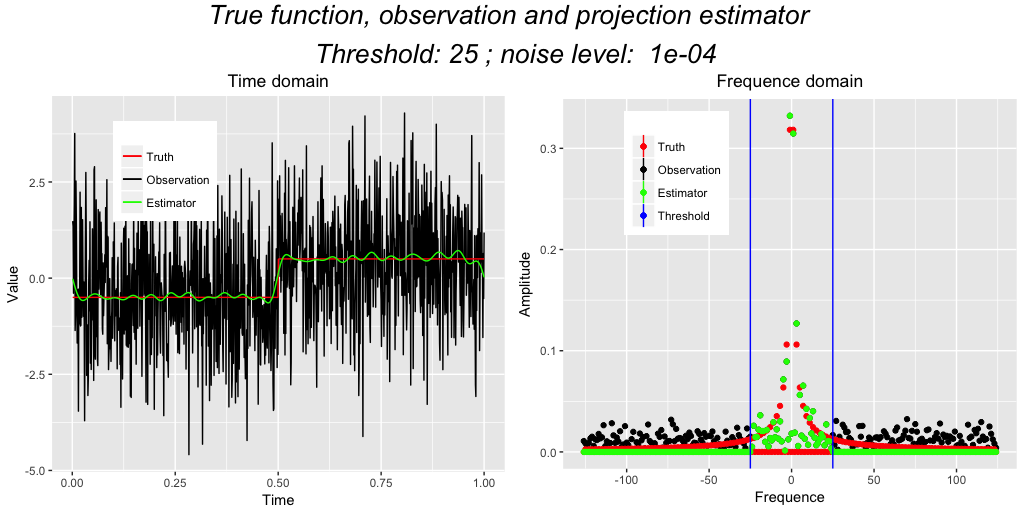
\includegraphics[width=1.\linewidth]{gauss/estimation/frequentist.png}
  \caption{Projection estimator in the time and frequency space, direct problem case.}
\label{igssm:estimation}
\end{figure}

Notice that, for any $m$ in $\N$, $\E[\Vert \theta^{\circ} - \theta_{n, \overline{m}} \Vert_{l^{2}}^{2}] = 2 \sum_{s \in \N} \E[(\Re(\theta^{\circ}(s)) - \Re(\theta_{n, \overline{m}}(s)))^{2}] + 2 \sum_{s \in \N} \E[(\Im(\theta^{\circ}(s)) - \Im(\theta_{n, \overline{m}}(s)))^{2}]$.
Hence, real and imaginary parts can be treated separately in an identical manner and considering the positive indexes is sufficient and we only will give attention to the estimation of the real part of the positively indexed coefficients of $\theta^{\circ}$ and we give this final formulation for the model.

\begin{de}\label{INTRO_IGSSM_DE}
Let $\Theta$ be the space of $\N^{\star}$-indexed, $\R$-valued sequences, equipped with the inner product $\langle \cdot \vert \cdot \rangle_{l^{2}} : ([x], [y]) \mapsto \sum_{s \in \N} [x](s) \cdot [y](s)$ and the associated norm $\Vert \cdot \Vert_{l^{2}}: [x] \mapsto \sum[x](s)^{2}$.
Let $\mathcal{L}^{2}$ be the subspace of $\Theta$ of square-summable sequences.

Given three elements of $\Theta$ denoted $\theta^{\circ}$, $\lambda$, and $\phi$, such that, $\phi = \theta^{\circ} \cdot \lambda$; for any $s$ in $\N$, $0 < \vert \lambda(s) \vert \leq 1$; and $\theta^{\circ}$ is an element of $\mathcal{L}^{2}$.

We observe $\phi_{n}$ in $\Theta$ such that, for any $s$ and $s'$ in $\N$ such that $s \neq s'$, we have $\phi_{n}(s) \sim \mathcal{N}(\phi(s), n^{-1})$ and $\Cov(\phi_{n}(s), \phi_{n}(s')) = 0$.
\assEnd
\end{de}

The likelihood for this model is given by
\[L(\phi_{n}, \theta) \propto \exp[n^{-1}(\sum\nolimits_{s \in \N} \phi_{n}(s) \theta(s) \lambda(s) - \sum\nolimits_{s \in \N} \Lambda(s)^{-1}\theta(s)^{2}/2)].\]

Notice that as in \nref{as:il}, $\V[\langle Y_{0}\vert e_{s} \rangle_{L^{2}}] = 1$, hence, all the results obtained considering the convergence rates remain true.
Hence let us give the following reminders.

\begin{nota*}
For any $m$ in $\mathds{N}^{\star}$; $s$ in $\mathds{N}^{\star}$; and $\theta$ in $\Theta$, let be the following quantities:
\begin{multline*}
\b_{m}^{2}(\theta) := \Vert \theta_{\underline{0}}\Vert_{l^{2}}^{-2} \Vert \theta_{\underline{m}} \Vert^{2}; \quad \Lambda(s) = \vert \lambda^{-1}(s) \vert^{2};\\
\Lambda_{\circ}(m) = m^{-1} \sum\nolimits_{0 < s \leq m} \Lambda(s); \quad \Lambda_{+}(m) := \max\nolimits_{s \in \llbracket 1, m \rrbracket}\{\Lambda(s)\}.
\end{multline*}
We then denote in the following way the risk for projection estimators:
\begin{equation*}
\mathcal{R}_{n}^{m}(\theta^{\circ}, \Lambda) := [n^{-1} m \Lambda_{\circ}(m) \vee \b_{m}^{2}(\theta^{\circ})].
\end{equation*}
Which gives us the following oracle rates,
\begin{multline*}
m^{\circ}_{n} \in \argmin\nolimits_{m \subset \mathds{M}}\left\{\mathcal{R}_{n}^{m}(\theta, \lambda)\right\} =  \argmin\nolimits_{m \subset \mathds{M}}\left\{[n^{-1} m \Lambda_{\circ}(m) \vee \b_{m}^{2}(\theta^{\circ})]\right\};\\
\mathcal{R}_{n}^{\circ}(\theta^{\circ}, \Lambda) = \mathcal{R}_{n}^{m_{n}^{\circ}}(\theta^{\circ}, \Lambda) = \min\nolimits_{m \in \N}\mathcal{R}_{n}^{m}(\theta^{\circ}, \Lambda).
\end{multline*}
And we were able to obtain the following maximal rates.
\begin{multline}
 \dRa{\Di}{\xdfCw[],\Lambda}:=[\xdfCw^2\vee\Di\oiSv \ssY^{-1}]:=\max\big(\xdfCw^2,\Di \oiSv \ssY^{-1}\big),\\
\hfill \mnDi(\xdfCw[]):=\mnDi(\xdfCw[],\Lambda):=\argmin\Nset[{\Di\in\N}]{\dRa{\Di}{\xdfCw[],\Lambda}}\quad\text{ and }\hfill\\\mnRa{\xdfCw[],\Lambda}:=\dRa{\mnDi({\xdfCw[]})}{\xdfCw[],\Lambda}=\min\Nset[{\Di\in\N}]{\dRa{\Di}{\xdfCw[],\Lambda}}.
\end{multline}
\assEnd
\end{nota*}

\begin{figure}
  \centering
  \begin{tabular}{@{}c@{}}
    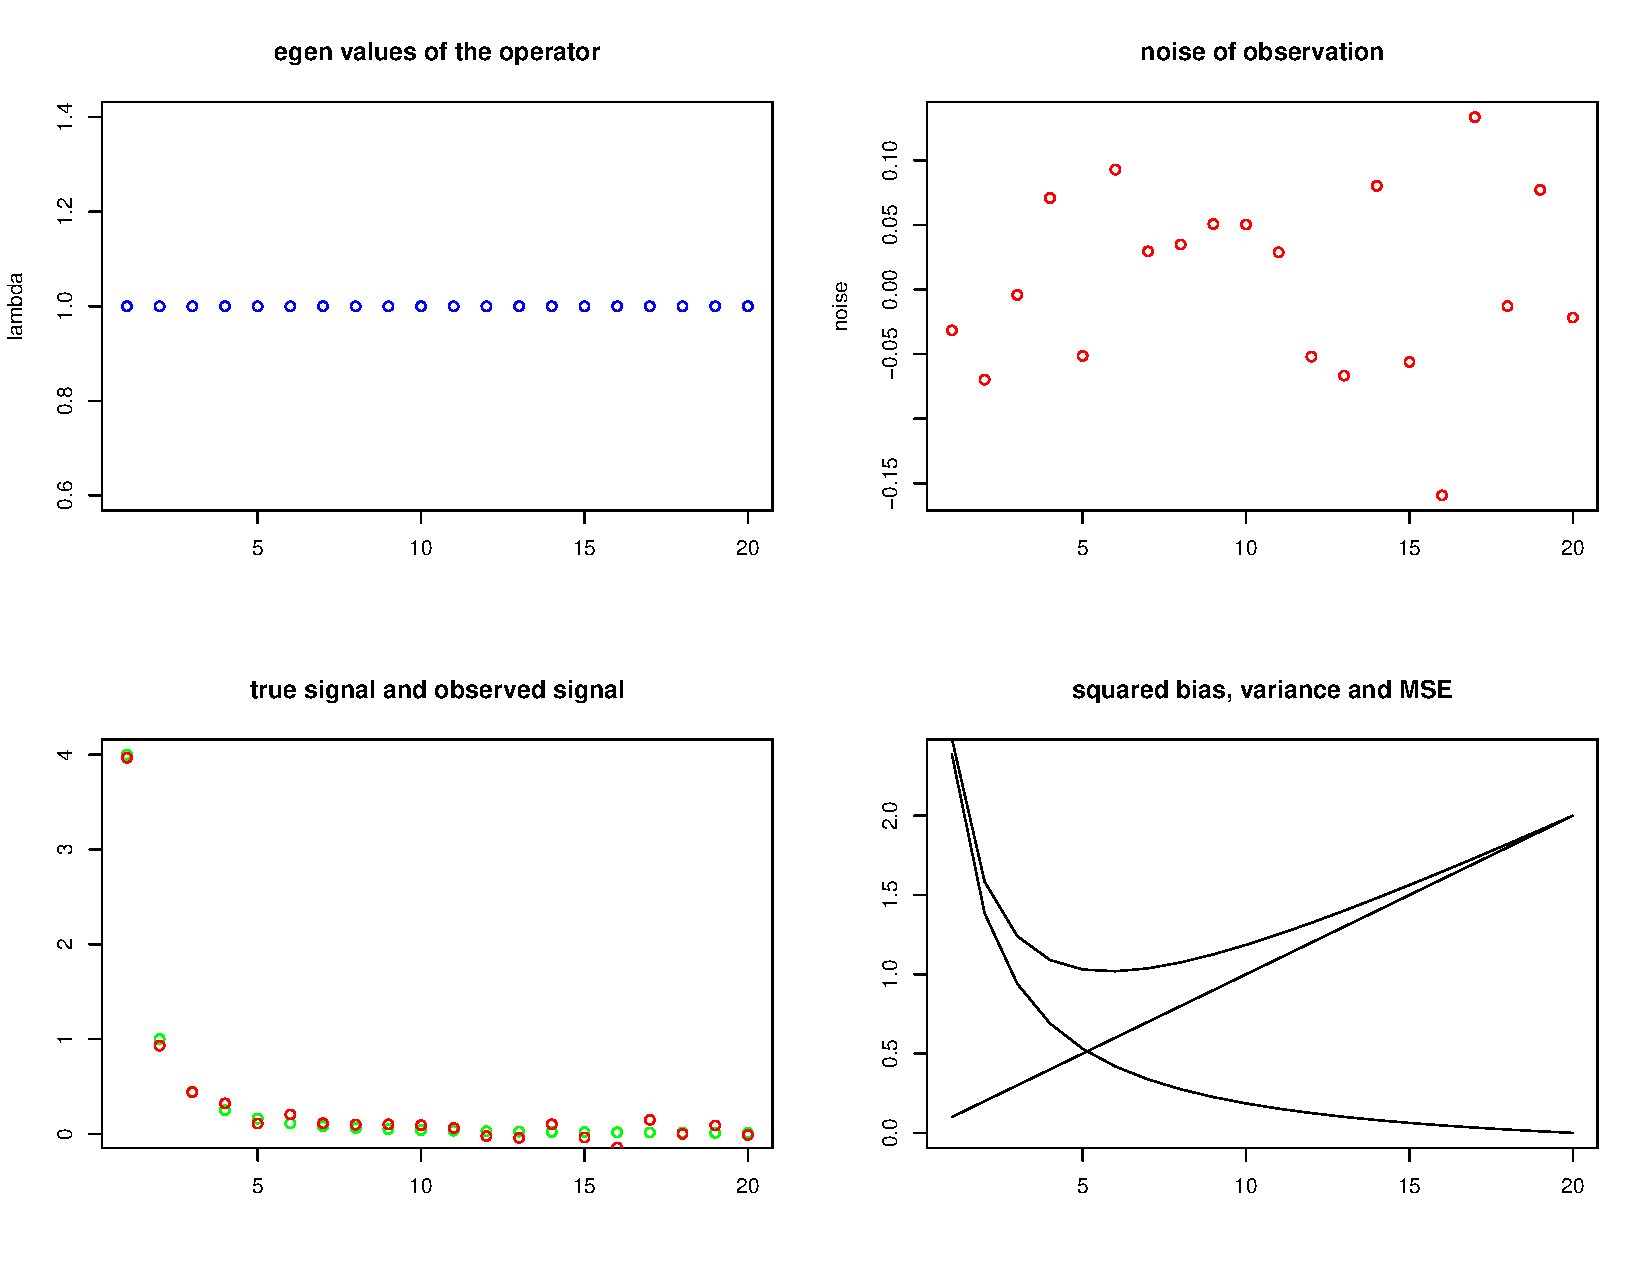
\includegraphics[width=.49\linewidth]{general/direct-case.pdf} \\[\abovecaptionskip]
  \end{tabular}
  \begin{tabular}{@{}c@{}}
    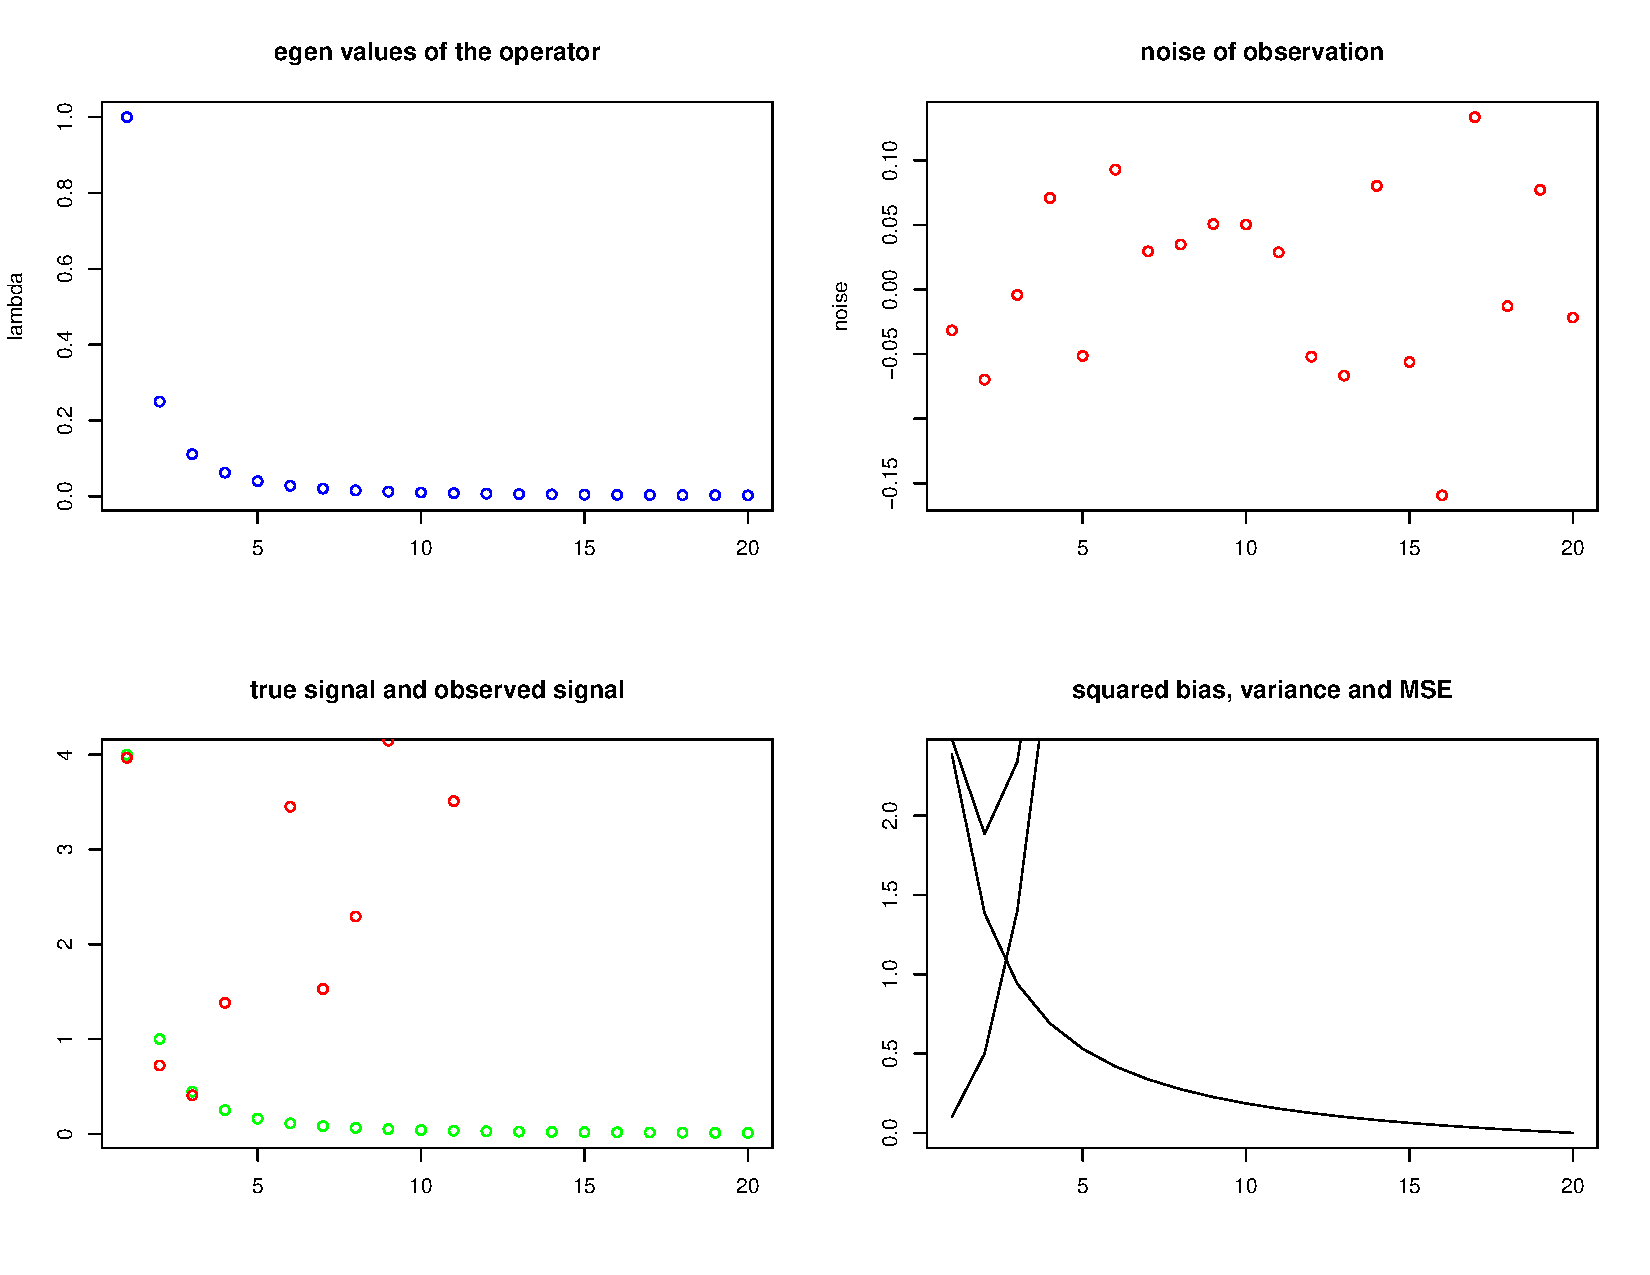
\includegraphics[width=.49\linewidth]{general/mildly-illposed.pdf} \\[\abovecaptionskip]
  \end{tabular}
  \caption{Influence of the operator Eigen-values sequence decay on the quadratic risk}\label{igssm:mildsev}
\end{figure}

\begin{rem*}
We shall emphasise that $\oRa{\xdf,\Lambda}\geq \ssY^{-1}$ for all
  $\ssY\in\N$, and
  
  $\lim_{n \rightarrow \infty} \oRa{\xdf,\Lambda}=0$.
  Observe that for all $\delta>0$ there exists $\Di_{\delta}\in\N$ and
  $\ssY_\delta\in\N$ such that for all $\ssY\geq \ssY_{\delta}$ holds
  $\bias[\Di_\delta]^2(\xdf)\leq \delta$ and
  $\Di_{\delta} \oiSv[\Di_\delta] \ssY^{-1}\leq\delta$, and whence
  $\oRa{\xdf,\Lambda}\leq\dRa{\Di_\delta}{\xdf,\Lambda}\leq \delta$.
  Moreover, we have $\oDi{\ssY}\in\nset{1,\ssY}$. Indeed, by construction
  holds
  $\bias[\ssY]^2(\xdf)\leq 1<(\ssY+1)\ssY^{-1}\leq
  (\ssY+1)\oiSv[\ssY+1]{}\ssY^{-1}$, and hence
  $\dRa{\ssY}{\xdf,\Lambda}<\dRa{\Di}{\xdf,\Lambda}$ for all
  $\Di\in \nsetro{\ssY+1,\infty}$ which in turn implies the claim
  $\oDi{\ssY}\in\nset{1,\ssY}$. Obviously, it follows thus
  $\oRa{\xdf,\Lambda}=\min\set{ \dRa{\Di}{\xdf,\Lambda}
    ,\Di\in\nset{1,\ssY}}$ for all $\ssY\in\N$. We shall use those
  elementary findings in the sequel without further reference.
The sequence $\mathcal{R}_{n}^{\circ}(\theta, \lambda)$ is then an exact oracle convergence rate and the projection estimator $\theta_{n, \overline{m_{n}^{\circ}}}$ is an oracle optimal estimator.

\medskip

Note that, in case \ref{oo:xdf:p}, the oracle rate is parametric, that is
$\oRa{\xdf, \Lambda} \approx \ssY^{-1}$. More precisely, if $\xdf=0$ then
for each  $\Di\in\N$,
$\E\Vnormlp{\txdfPr-\xdf}^2=\Di\oiSv[\Di]\ssY^{-1}$,
and hence $\oDi{\ssY}=1$ and $\oRa{\xdf, \Lambda}=2\oiSv[1]\ssY^{-1}\sim\ssY^{-1}$. Otherwise
if there is $K\in\N$  with $\bias[K-1](\xdf)>0$ and
$\bias[K](\xdf)=0$, then setting
$\ssY_{\xdf}:=\tfrac{K\oiSv[K]}{\bias[K-1]^2(\xdf)}$, for all
$\ssY\geq \ssY_{\xdf}$ holds
$\bias[K-1]^2(\xdf)>K\oiSv[K]\ssY^{-1}$, and hence  $\oDi{\ssY}=K$ and
$\oRa{\xdf,\Lambda}= K\oiSv[K]\ssY^{-1}\sim \ssY^{-1}$.
On the other hand side, in case \ref{oo:xdf:np} the oracle rate is
non-parametric, more precisely, it holds
$\lim_{\ssY\to\infty}\ssY\oRa{\xdf,\Lambda}=\infty$. Indeed, since
$\bias[\oDi{\ssY}]^2(\xdf)\leq\oRa{\xdf,\Lambda}=\oRa{\xdf,\Lambda}\in\mathfrak{o}_{n}(1)$ follows $\oDi{\ssY}\to\infty$ and hence
$\oDi{\ssY}\oiSv[\oDi{\ssY}]\to\infty$ which implies the claim because
$\ssY\oRa{\xdf,\Lambda}\geq\oDi{\ssY}\oiSv[\oDi{\ssY}]$.

\medskip

When considering the maximal rate, by construction it holds 
$\mnRa{\xdfCw[],\Lambda}\geq \ssY^{-1}$ for all $\ssY\in\N$.
The following statements can be
shown using the same arguments as in \nref{oo:rem:ora}
by exploiting that the sequence $\xdfCw[]$ is assumed to be
non-increasing, strictly positive with limit zero and $\xdfCw[(1)]=1$. 
Thereby, we conclude that 
$\mnRa{\xdfCw[],\Lambda}=\mathfrak{o}_{n}(1)$ and $\ssY\mnRa{\xdfCw[],\Lambda}\to\infty$ as well as 
$\mnDi(\xdfCw[])\in\nset{1,\ssY}$ for all $\ssY\in\N$. It follows also that
$\mnDi(\xdfCw[])=\argmin\Nset[{\Di\in\nset{1,n}}]{\dRa{\Di}{\xdfCw[],\Lambda}}$ and 
$\mnRa{\xdfCw[],\Lambda}=\min\Nset[{\Di\in\nset{1,n}}]{\dRa{\Di}{\xdfCw[],\Lambda}}$ for all
$\ssY\in\N$. We shall stress that in this situation the rate
$\mnRa{\xdfCw[],\Lambda}$ is non-parametric.
\remEnd
\end{rem*}

We give in \nref{igssm:oracle} an illustration of the oracle estimator in a Gaussian sequence space model, in the direct problem case that is to say $\lambda(s) = 1$ for all $s$ in $\N$.

\begin{figure}
  \centering
  \begin{tabular}{@{}c@{}}
    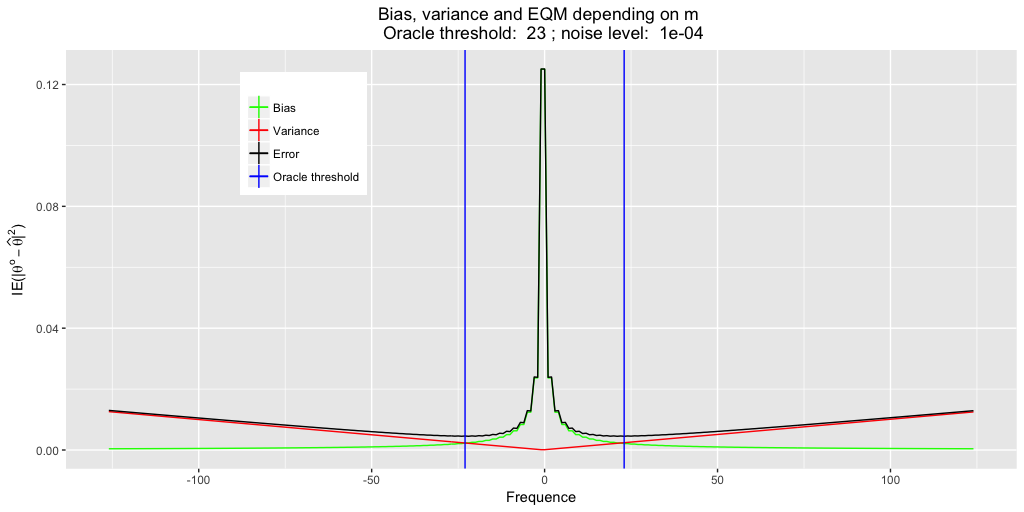
\includegraphics[width=.49\linewidth]{gauss/error/oracle_threshold.png} \\[\abovecaptionskip]
  \end{tabular}
  \begin{tabular}{@{}c@{}}
    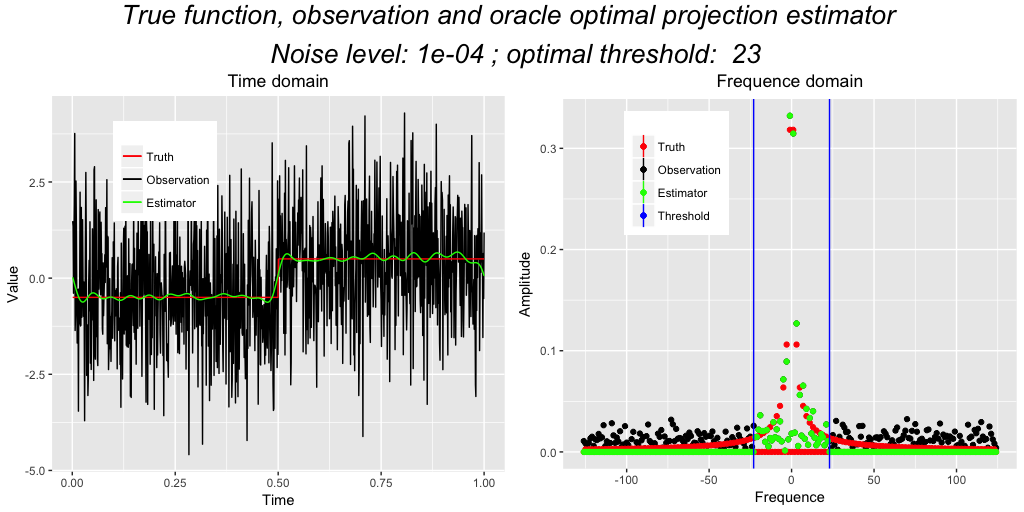
\includegraphics[width=.49\linewidth]{gauss/error/oracle_estimator.png} \\[\abovecaptionskip]
  \end{tabular}
  \caption{Illustration of the oracle value for $m$ and associated projection estimator.}\label{igssm:oracle}
\end{figure}

\subsection{Unknown operator}
In the case of an unknown operator, that is, $h$, and hence, $\lambda$ unknown, we supposed that, in addition to $Y$ we define another Gaussian process $\epsilon$.
Let $\epsilon$ be the Gaussian process such that for any $t$ in $[0, 1]$, we have $\d \epsilon(t) = \d W(t) + h(t) \d t$ where $W$ is the Brownian motion.
Hence, there exist sequences of real-valued random variables $(\xi_{3}(s))_{s \in \Z}$ and $(\xi_{4}(s))_{s \in \Z}$ such that for any $s$ and $s'$ in $\Z$, we have $\int_{[0, 1]} e_{s}(t) \d \epsilon(t) = \int_{[0, 1]} \cos(2 \pi s t) \d W(t) + \imath \int_{[0, 1]} \sin(2 \pi s t) \d W(t) + \lambda(s) = \xi_{3}(s) + \imath \xi_{4}(s) + \phi(s)$ with $\xi_{3}(s) \sim \mathcal{N}(0, 1/2)$, $\xi_{4}(s) \sim \mathcal{N}(0, 1/2)$, and $\xi_{3}(s)$ is independent of $\xi_{4}(s)$, in addition, $\Cov(\xi_{3}(s), \xi_{3}(s')) = \mathds{1}_{\{\vert s' \vert = \vert s \vert\}}$ and $\Cov(\xi_{4}(s), \xi_{4}(s')) = \text{Sign}(s \cdot s') \mathds{1}_{\{\vert s' \vert = \vert s \vert\}}$.
Define the \iid stochastic process $(\epsilon_{p})_{p \in \Z}$ such that, for any $p$ in $\Z$, $\epsilon_{p}$ is identically distributed to $\epsilon$.
We observe the sub-vector $\epsilon^{n_{\lambda}} = (\epsilon_{p})_{p \in \llbracket 1, n_{\lambda} \rrbracket}$ of $(\epsilon_{p})_{p \in \Z}$ and define, for any $s$ in $\N$ the estimates

$\lambda_{\ssE}(s) = \sum_{p = 1}^{n_{\lambda}} \int_{[0, 1]} e_{s}(t) \d \epsilon(t) \ssE^{-1}$ which verifies $\Re(\lambda_{\ssE}(s)) \sim \mathcal{N}(\Re(\lambda(s)), 2\ssE^{-1})$ and $\Im(\lambda_{\ssE}(s)) \sim \mathcal{N}(\Im(\lambda(s)), 2 \ssE^{-1})$ so we define $\theta_{\ssY, \ssE}(s) := \phi_{n}(s) \lambda_{\ssE}^{+}(s)$, with $\lambda_{\ssE}^{+}(s) = \lambda_{\ssE}^{-1}(s) \mathds{1}_{\{\vert \lambda_{\ssE}\vert^{2} \geq \ssE^{-1}\}}$.

We may carry the same observations about the convergence rate and hence we give the following final definition for the model in the case of unknown operator.
\begin{de}\label{INTRO_IGSSM_DE_UK}
Let $\Theta$ be the space of $\N$-indexed, $\R$-valued sequences, equipped with the inner product $\langle \cdot \vert \cdot \rangle_{l^{2}} : ([x], [y]) \mapsto \sum_{s \in \N} [x](s) \cdot [y](s)$ and the associated norm $\Vert \cdot \Vert_{l^{2}}: [x] \mapsto \sum[x](s)^{2}$.
Let $\mathcal{L}^{2}$ be the subspace of $\Theta$ of square-summable sequences.

Given three elements of $\Theta$ denoted $\theta^{\circ}$, $\lambda$, and $\phi$, such that, $\phi = \theta^{\circ} \cdot \lambda$; for any $s$ in $\N$, $0 < \vert \lambda(s) \vert \leq 1$; and $\theta^{\circ}$ is an element of $\mathcal{L}^{2}$.

We observe the $\Theta$-valued random variable $\phi_{n}$  such that, for any $s$ and $s'$ in $\N$ such that $s \neq s'$, we have $\phi_{n}(s) \sim \mathcal{N}(\phi(s), n^{-1})$ and $\Cov(\phi_{n}(s), \phi_{n}(s')) = 0$.
On the other hand, we also observe the $\Theta$-valued random variable $\lambda_{\ssE}$ such that, for any $s$ and $s'$ in $\N$ such that $s \neq s'$, we have $\lambda_{\ssE}(s) \sim \mathcal{N}(\lambda(s), \ssE^{-1})$ and $\Cov(\lambda_{\ssE}(s), \lambda_{\ssE}(s')) = 0$.
\assEnd
\end{de}

As a direct consequence we have for any $s$ in $\N^{\star}$, as in \nref{as:il}, $\lambda(s) - \lambda_{\ssE}(s) \sim \mathcal{N}(0, \ssE^{-1})$ and hence, $\ssE^{2} \E\vert \lambda(s) - \lambda_{\ssE}(s) \vert^{4} = 3$ and $n_{\lambda} \E[\vert \lambda_{\ssE}(s) - \lambda(s) \vert^{2}] = 1$.
Hence, \nref{as:il} holds true and the analysis of the optimal rates carried out previously still holds true.
We hence remind the following results we obtained.

\begin{nota*}
In addition to the case of a known operator, we defined the following rate, for all $\ssE$ in $N$
\begin{multline*}
\mathcal{R}_{n_{\lambda}}^{\dagger}(\theta^{\circ}, \Lambda) := \sum_{s \in \mathds{F}}\vert \theta(s) \vert^{2} (1 \wedge n_{\lambda}^{-1} \Lambda(s))\\
\mmRa{\xdfCw[],\Lambda}:=\max_{s\in\N}\{\xdfCw[(s)]^2[1\wedge \iSv[s]/\ssE]\}\Vnorm[1/{\xdfCw[]}]{\xdf}^2.
\end{multline*}
\end{nota*}

\begin{rem*}
We have
\begin{equation*}
\mathcal{R}_{n, n_{\lambda}}(\theta_{n, n_{\lambda}, \overline{m_{n}^{\circ}}}) \leq (1 + \Vert \theta^{\circ}_{\underline{0}} \Vert_{l^{2}}^{2})\mathcal{R}_{n}^{\circ}(\theta^{\circ}, \Lambda) + 2 \mathcal{R}_{n_{\lambda}}^{\dagger}(\theta^{\circ}, \Lambda).
\end{equation*}
We note that $\Vnormlp{\xdf_{\underline{0}}}^2=0$ implies
  $\mRa{\xdf,\Lambda}=0$, while for $\Vnormlp{\xdf_{\underline{0}}}^2>0$ holds
  $\mRa{\xdf,\Lambda}\geq \sum_{s:\iSv[s]>\ssE} \vert \fxdf[(s)] \vert ^2+\ssE^{-1}\sum_{s:\iSv[s]\leq\ssE} \vert \fxdf[(s)] \vert ^2  \geq\ssE^{-1}\sum_{s\in\N} \vert \fxdf[(s)] \vert ^2=\Vnormlp{\xdf_{\underline{0}}}^2
  \ssE^{-1}$, thereby whenever $\xdf\ne 0$
  any additional term of order $\ssY^{-1}+\ssE^{-1}$
  is negligible with respect to the rate
  $\oRa{\xdf,\Lambda}+\mRa{\xdf,\Lambda}$, since
  $\oRa{\xdf,\Lambda}\geq \ssY^{-1}$, 
  which we will use below without further reference. We shall
  emphasise that in case $\ssY=\ssE$ it holds
  \begin{multline}
    \mRa[\ssY]{\xdf,\Lambda}=\sum_{0 < s \leq m_{n}^{\circ}} \vert \fxdf[(s)] \vert^2 [1 \wedge \ssY^{-1}\iSv[s]]
    + \sum_{s > m_{n}^{\circ}} \vert \fxdf[(s)] \vert ^2[1\wedge\ssY^{-1}\iSv[s]]\\
    \leq \cst{}\Vnormlp{\xdf_{\underline{0}}}^2 \ssY^{-1} \oDi{\ssY}
    \oiSv[\oDi{\ssY}] +
    \cst{}\Vnormlp{\xdf_{\underline{0}}}^2\bias[\oDi{\ssY}]^2(\theta^{\circ})\leq
    \Vnormlp{\xdf_{\underline{0}}}^2\dRa{\oDi{\ssY}}{\xdf,\Lambda}
  \end{multline}
  which in turn implies $\mathcal{R}_{n, n_{\lambda}}(\theta_{n, n_{\lambda}, \overline{m_{n}^{\circ}}}) \leq 4 \Vert \theta^{\circ}_{\underline{0}} \Vert_{l^{2}}^{2}\mathcal{R}_{n}^{\circ}(\theta^{\circ}, \Lambda)$.
  In other words, the estimation of the unknown operator $T$ is negligible whenever $\ssY\leq\ssE$.
  
  \medskip
  
Considering then the behaviour of the oracle rate, we have the following results.
We note that in case \ref{oo:xdf:p}
$\mRa{\xdf,\Lambda}\leq
\Vnormlp{\xdf_{\underline{0}}}^2\miSv[K]\ssE^{-1}$
and hence
\begin{equation}
 \nmRi{\hxdfPr[\oDi{\ssY}]}{\xdf,\Lambda}
 % \FuEx\Vnormlp{\hxdfPr[\oDi{\ssY}]-\xdf}^2
 \leq
\{[1\vee\Vnormlp{\xdf_{\underline{0}}}^2]\{
K\oiSv[K]\ssY^{-1}+\miSv[K]\ssE^{-1}\}
\end{equation}
for all $\ssE\in\N$ and $\ssY\geq\ssY_{\xdf}$ with $\ssY_{\xdf}$ as in \nref{oo:rem:ora}. In other words the
rate is parametric in both the $\rE$-sample size $\ssE$ and the $\rY$-sample size $\ssY$. Thereby, the  additional estimation of $\lambda$ is negligible whenever $\ssE\geq\ssY$.  In the
opposite case \ref{oo:xdf:np}, it is obviously of interest to characterise the minimal size $\ssE$ of the additional
sample from $\rE$ needed to attain the same rate as in case of a known
operator. We carried this discussion in \nref{ge:il:oo:kn}.

\medskip

On the other hand, if one is interested in the maximal risk, we have the following results.
For all $\ssE\in\N$ holds
$\sup_{\xdf\in\rwCxdf}\oRa{\xdf,\Lambda}\leq
\xdfCr^2\mmRa{\xdfCw[],\Lambda}$, since for all
$\xdf\in\rwCxdf$ 
\begin{equation}
  \mmRa{\xdf,\Lambda}=\sum_{s\in\N^{\star}} \vert \fxdf[(s)] \vert ^2[1\wedge \iSv[s]/\ssE]\leq
\max_{s\in\N}\{\xdfCw[(s)]^2\min(1,\iSv[s]/\ssE)\}\Vnorm[1/{\xdfCw[]}]{\xdf}^2.
\end{equation}
It follows for all $\Di,\ssY,\ssE\in\N$ immediately that 
\begin{equation}
  \nmRi{\hxdfPr}{\rwCxdf,\Lambda}
  \leq (\xdfCr^2+8) \dRa{\Di}{\xdfCw[],\Lambda}+16\xdfCr^2\mmRa{\xdfCw[],\Lambda}.
\end{equation}
The upper bound in the last display depends on the dimension parameter
$\Di$ and hence by choosing an optimal value $\mnDi$ as in
\eqref{mm:de:nra} the upper bound
will be minimised, that is
\begin{equation}
  \nmRi{\hxdfPr[\mnDi]}{\rwCxdf,\Lambda}
  \leq (\xdfCr^2+8) \mnRa{\xdfCw[],\Lambda}+16\xdfCr^2\mmRa{\xdfCw[],\Lambda}.
\end{equation}

\medskip

 Since the operator $T$ is not known, it is natural to
  consider a maximal risk also over a class for $\edf$ characterising the behaviour of
  $\Nsuite[s]{\iSv[s]= \vert \fedf[(s)] \vert ^{-2}}$, precisely $\rwCedf:=\{\edf\in\lp[2]:\edfCr^{-2}\leq\edfCw[s] \vert \fedf[(s)] \vert ^{2}=
\edfCw[s]\iSv[ s ]^{-1}\leq \edfCr^{2},\;\forall s\in\N^{\star}\}$.
We shall note that for all $\Di\in\N$ and any $\edf\in\rwCedf$,
$\edfCr^{-2}\leq\miSv/\edfCwm\leq \edfCr^{2}$,
$\edfCr^{-2}\leq\oiSv/\edfCwo\leq \edfCr^{2}$. Setting
for all $\ssY,\ssE\in\N$
\begin{multline}
 \dRa{\Di}{\xdfCw[],\edfCw[]}:=[\xdfCw^2\vee\Di\edfCwo \ssY^{-1}],
\hfill
\mnDi(\xdfCw[],\edfCw[]):=\argmin\Nset[{\Di\in\N}]{\dRa{\Di}{\xdfCw[],\edfCw[]}},\hfill\\\mnRa{\xdfCw[],\edfCw[]}:=\dRa{\mnDi({\xdfCw[],\edfCw[]})}{\xdfCw[],\edfCw[]}=\min\Nset[{\Di\in\N}]{\dRa{\Di}{\xdfCw[],\edfCw[]}}\quad\text{
  and }\\
\mnRa{\xdfCw[],\edfCw[]}:=\max\{\xdfCw[(s)]\min(1,\edfCw[s]/\ssE),s\in\N\}.
\end{multline}
we have 
\begin{multline}
 \mnRa{\xdfCw[],\Lambda}=\min_{\Di\in\N}\{[\xdfCw\vee\Di\oiSv\ssY^{-1}]\}\leq
 \edfCr^2\min_{\Di\in\N}\{[\xdfCw\vee\Di\edfCwo\ssY^{-1}]\}\leq \edfCr^2\dRa{\Di}{\xdfCw[],\edfCw[]}\\ 
  \mmRa{\xdfCw[],\Lambda}=\max_{s\in\N}\{\xdfCw[(s)]^2[1\wedge \iSv[s]/\ssE]\}\leq\edfCr^2\mnRa{\xdfCw[],\edfCw[]}.
\end{multline}
It follows for all $\Di,\ssY\in\N$ immediately that 
\begin{equation}
  \nmRi{\hxdfPr}{\rwCxdf,\rwCedf}
  \leq (\xdfCr^2+8\edfCr^2) \mnRa{\xdfCw[],\edfCw[]}
+8(\cst{4}+1)\edfCr^2\xdfCr^2\mmRa{\xdfCw[],\edfCw[]}.
\end{equation}
\ncite{JohannesSchwarz2013a} have shown  that
  $\inf_{\hxdf}\nmRi{\hxdf}{\rwCxdf,\rwCedf}$, where the infimum is taken over all
  possible estimators $\hxdf$ of $\xdf$, is up to a constant bounded
  from below by $\mnRa{\xdfCw[],\edfCw[]}\vee\mmRa{\xdfCw[],\edfCw[]} $.  Consequently, the rate
  $\Nsuite[n]{\mnRa{\xdfCw[],\edfCw[]}\vee\mmRa{\xdfCw[],\edfCw[]}}$, the dimension parameters $\Nsuite[n]{\mnDi(\xdfCw[])}$
  and the projection estimators $\Nsuite[n]{\txdfPr[\mnDi({\xdfCw[]})]}$, respectively, is a
  minimax rate, a minimax dimension and minimax optimal (up to a
  constant).
\remEnd
\end{rem*}
We place ourselves in the framework introduced in \nref{INTRO_CIRCULARDECONVOLUTION}.
We will first consider the case of a known operator, first with independent data, then with an absolutely regular process.
We will then consider an unknown operator.
In all cases, we start by giving the explicit, detailed expression of the estimator, as well as the sequence which shall be proven o be an upper bound for the quadratic risk, before reminding the hypotheses to prove in order to obtain the convergence, we shall then proceed to show that the said hypothesis holds true before concluding.
The proofs for the results obtained in this section may be found in \nref{a:prel}.


 %======================================================================================================================
%                                                                 
% Title:  Aggregated CDE: known error density
% Author: Jan JOHANNES, Institut für Angewandte Mathematik, Ruprecht-Karls Universität Heidelberg, Deutschland  
% 
% Email: johannes@math.uni-heidelberg.de
% Date: %%ts latex start%%[2018-03-29 Thu 12:11]%%ts latex end%%
%
% ======================================================================================================================
% --------------------------------------------------------------------
% section <<Aggregated CDE: known error density>>\nref{ak}
% --------------------------------------------------------------------
\subsection{Independent data and known convolution density}\label{FREQ_DECONV_KNOWN}\label{ak:rb}\label{AK:RB}
% ....................................................................
% <<Text Aggregated CDE>>
% ....................................................................
\begin{te}
We place ourselves under \nref{AS_INTRO_DATA_KNOWN} and \nref{AS_INTRO_DATA_INDEPENDENT} and intend to apply the strategy highlighted in \nref{freq:ge:strat:kn}.
\end{te}

We assume here that we know $\lambda$ and observe the vector of independent random variables $Y^{n}$.
Assume now that for any $s$ in $\N$, we know $\lambda(s)$ and $\lambda(s) > 0$.
\subsubsection{Shape of the estimator}
First, let us remind that we plan to use an aggregated orthogonal series estimator $\widehat{\theta}^{(\eta)}$, with $\eta$ in $\R_{+}^{\star} \cup \infty$ which form is reminded hereafter.
\begin{de*}
We first define so-called contrast $\Upsilon$ and penalisation $\pen^{\Lambda}$ sequences, which allow us to define weight $\P_{M}^{(\eta)}$ on the nested sieve space (here $(\llbracket 0, m \rrbracket)_{m \in \N}$)
\begin{multline*}
\Upsilon : \mathds{N} \to \R_{+}, \quad m \mapsto \Upsilon(m); \qquad \pen^{\Lambda} : \N \to \R_{-}, \quad m \mapsto \pen^{\Lambda}(m);\\
\P_{M}^{(\eta)} : \N \to \R_{+}, \quad m \mapsto \tfrac{\exp[\eta n (\Upsilon(m) + \pen^{\Lambda}(m))]}{\sum\nolimits_{k = 0}^{n} \exp[\eta n (\Upsilon(k) + \pen^{\Lambda}(k))]} \mathds{1}_{m \leq n}.
\end{multline*}
Notice that letting $\eta$ tend to $\infty$ in the previous definition gives rise to the penalised contrast model selection estimator,
\begin{equation*}
  \tDi:=\argmin\nolimits_{\Di\in\nset{1,\ssY}} \big\{\Upsilon(m) + \penSv\big\}
\end{equation*}
which corresponds to the following weights
\begin{equation*}
  \lim\nolimits_{\rWc\to\infty}\rWe=\dirac[\tDi](\{\Di\})=:\msWe.
\end{equation*}
Here, we will use the following shape for $\Upsilon$ and $\pen^{\Lambda}$, for $\cpen := 84$
\begin{alignat*}{4}
  & \Upsilon(m) && := && \Vert \theta_{n, \overline{m}} \Vert_{l^{2}}^{2};  \quad && \cmiSv := \tfrac{\log^{2}(\Di\miSv \vee(\Di+2))}{\log^{2}(\Di+2)}\geq1;\\
  & \DipenSv && := && \cmiSv \Di \miSv; \quad && \penSv:= \penD.
  \end{alignat*}
  \assEnd
\end{de*}
The family of estimators is hence entirely defined and can be implemented with the data we assume to have at hand in this subsection.
  
 \subsubsection{Quadratic risk bounds of the aggregated estimator}\label{AK:RB:OR}
 In a first time we are interested in the quadratic risk for any $\theta^{\circ}$ fixed.
Remind that the strategy we use allows to show that the following sequence is an upper bound for the quadratic risk.
\begin{de*}
Remind that we defined for any $\theta$ in $\Theta$ and $\Di$ in $\N$ the following term $\b_{m}^{2}(\theta) = \Vert \theta_{\underline{m}} \Vert_{l^{2}}/\Vert \theta_{\underline{0}} \Vert_{l^{2}} \leq 1$.
We then define a family of sequences $(\daRa{\Di}{(\xdf)})_{\Di \in \N} := (\daRa{\Di}{(\xdf,\Lambda)})_{\Di \in \N} = [\b_{m}^{2}(\theta^{\circ}) \vee \penSv/\cpen]$ and hence it holds for all $\Di$ in $\nset{1,\ssY}$
    \begin{equation}
      [\Vnormlp{\xdf_{\underline{0}}}^2+\cpen]\daRa{\Di}{(\xdf)}\geq\Vnormlp{\xdf_{\underline{0}}}^2\bias^2(\xdf)\vee\penSv.
      \end{equation}
We intend to prove that the specific choice
\begin{multline*}
\aDi{\ssY}(\xdf):=\argmin\Nset[\Di\in\Nz]{\daRa{\Di}{(\xdf)}}\in\nset{1,\ssY}; \\
\naRa{(\xdf)}:=\naRa{(\xdf,\Lambda)}:=\min\Nset[\Di\in\Nz]{\daRa{\Di}{(\xdf)}}
\end{multline*}
with $\daRa{\aDi{\ssY}}{(\xdf,\Lambda)}=\naRa{(\xdf,\Lambda)}$ defines an upper bound for the convergence rate of the aggregation estimators.
\assEnd
\end{de*}
 
The following lemma shows that the assumption for our method is verified.
\begin{lm}\label{re:conc}
  Let $\oiSv=\tfrac{1}{\Di}\sum_{s\in\nset{1,\Di}}\iSv[s]$,
  $\miSv= \max\{\iSv[s],s\in\nset{1,\Di}\}$, $\cmSv\geq1$ and
  $\DipenSv=\cmSv\Di \miSv$, then there is a numerical constant
  $\cst{}$ such that for all $\ssY\in\Nz$ and
  $\Di\in\nset{1,\ssY}$ holds
  \begin{resListeN}[]
  \item\label{re:conc:i}
    $\E \vectp{\Vnormlp{\txdfPr-\xdfPr}^2 - 12\DipenSv\ssY^{-1}}\\
    \leq 
    \cst{} \bigg[\tfrac{\Vnormlp[1]{\fydf}\,\miSv}{\ssY}\exp\big(\tfrac{-\cmSv\Di}{3\Vnormlp[1]{\fydf}}\big)+\tfrac{2\Di\miSv}{n^2}\exp\big(\tfrac{-\sqrt{n\cmSv}}{200}\big) \bigg]$
  \item\label{re:conc:ii}
    $\P\big(\Vnormlp{\txdfPr-\xdfPr}^2 \geq 12\DipenSv\ssY^{-1}\big)\leq 
    3 \bigg[\exp\big(\tfrac{-\cmSv\Di}{200\Vnormlp[1]{\fydf}}\big)
    +\exp\big(\tfrac{-\sqrt{\ssY\cmSv}}{200}\big)\bigg]$
  \item\label{re:conc:iii}
    $\P\big(\Vnormlp{\txdfPr-\xdfPr}^2 \geq 12\daRa{\Di}{(\xdf,\Lambda)}\big)\leq 
    3 \bigg[\exp\big(\tfrac{-\ssY\daRa{\Di}{(\xdf,\Lambda)}}{200\Vnormlp[1]{\fydf}\miSv}\big)
    +\exp\big(\tfrac{-\ssY\sqrt{\daRa{\Di}{(\xdf,\Lambda)}}}{200\sqrt{\Di\miSv}}\big)\bigg]$
  \end{resListeN}
\end{lm}

Hence, using \nref{freq:ge:strat:kn:qu:pnp} gives us the following result.
% ....................................................................
% <<Re upper bound ag p np>>
% ....................................................................
\begin{thm}
Consider the penalty sequence $\penSv:=\penD$, $\Di\in\nset{1,n}$, as in \nref{freq:ge:shape:kn:de:pen:oo} with numerical constant $\cpen \geq 84$.
Let $\txdfAg[{\erWe[]}]=\sum_{\Di=1}^{\ssY}\We\txdfPr$ be an aggregation of the orthogonal series estimators, using either aggregation weights $\rWe[]$ as in \eqref{freq:ge:shape:kn:we}, or model selection weights $\msWe[]$ as in \eqref{freq:ge:shape:kn:de:msWe}.
\begin{Liste}[]
\item[{\dgrau\bfseries{(p)}}]Assume there is $K\in\Nz$
  with   $1\geq \bias[{[K-1] }](\xdf)>0$ and $\bias[\Di](\xdf)=0$. For
  $K>0$ let
  $ c_{\xdf}:=\tfrac{\Vnormlp{\xdf_{\underline{0}}}^2+4\cpen}{\Vnormlp{\xdf_{\underline{0}}}^2\bias[{[K-1]}]^2(\xdf)}>1$ and
  $\ssY_{\xdf}:=\gauss{c_{\xdf}\DipenSv[K]}\in\Nz$. If
  $\ssY\in\nset{1,\ssY_{\xdf}}$ then set $\sDi{\ssY}:=\Di_{\cst{3}}\log(\ssY)$, and otherwise if
  $\ssY>\ssY_{\xdf}$ then set
  $\sDi{\ssY}:=\max\{\Di\in\nset{K,\ssY}:\ssY>c_{\xdf}\DipenSv\}$
  where the defining set contains $K$ and thus is not empty.
There is a finite constant $\cst{\xdf,\Lambda}$
given in \eqref{ak:ag:ub:pnp:p7} depending only on $\xdf$ and $\Lambda$ such that for all $n\in\Nz$ holds
\begin{equation}
  \nRi{\txdfAg[{\erWe[]}]}{\xdf,\Lambda}
  % \E\Vnormlp{\txdfAg[{\erWe[]}]-\xdf}^2
  \leq
  \cst{}\Vnormlp{\xdf_{\underline{0}}}^2\big[
  \ssY^{-1}\vee\exp\big(-2\cmiSv[\sDi{\ssY}]\sDi{\ssY}\big)\big]
  + \cst{\xdf,\Lambda}\ssY^{-1}.
\end{equation}
\item[{\dgrau\bfseries{(np)}}] Assume that
  $\bias(\xdf)>0$ for all  $\Di\in\Nz$.
There is a finite finite constant $\cst{\xdf,\Lambda}$ given in
\eqref{ak:ag:ub:pnp:p8} depending only $\xdf$ and $\Lambda$ such that for all
$\ssY\in\Nz$  holds 
 \begin{equation}
   \nRi{\txdfAg[{\erWe[]}]}{\xdf,\Lambda}
   % \E\Vnormlp{\txdfAg[{\erWe[]}]-\xdf}^2
    \leq 
   \cst{}(\Vnormlp{\xdf_{\underline{0}}}^2\vee1)\min_{\Di\in\nset{1,\ssY}}\big[\dRa{\Di}{\xdf,\Lambda}\vee\exp\big(-2\cmiSv\Di\big)\big]\\
   +\cst{\xdf,\Lambda}\ssY^{-1}.
\end{equation}
\end{Liste} 
\reEnd 
\end{thm}

\begin{cor}
  Let $\cpen \geq 84$.
  \begin{Liste}[]
  \item[{\dgrau\bfseries{(p)}}]
    If in addition
    \begin{inparaenum}\item[{{\dgrau\bfseries(A1)}}]
      there is $\ssY_{\xdf,\Lambda}\in\Nz$ such that
      $\cmiSv[\sDi{\ssY}]\sDi{\ssY}\geq (\log\ssY)/2$ for all
      $\ssY\geq \ssY_{\xdf,\Lambda}$
    \end{inparaenum}
    holds true, then there is a constant $\cst{\xdf,\Lambda}$ depending
    only on $\xdf$ and $\Lambda$ such that for all $n\in\Nz$ holds
    $\nRi{\txdfAg[{\erWe[]}]}{\xdf,\Lambda} \leq
    \cst{\xdf,\Lambda}\ssY^{-1}$.
  \item[{\dgrau\bfseries{(np)}}]
    If in addition
    \begin{inparaenum}\item[{{\dgrau\bfseries(A2)}}]
      there is  $\ssY_{\xdf,\Lambda}\in\Nz$ such that
      $\aDi{\ssY}(\xdf)\cmSv[\aDi{\ssY}(\xdf)]\geq \vert \log\naRa{(\xdf,\Lambda)} \vert/2 $
      for all $\ssY\geq \ssY_{\xdf,\Lambda}$
    \end{inparaenum}
    holds true, then there is a constant $\cst{\xdf,\Lambda}$ depending
    only on $\xdf$ and $\Lambda$ such that $\nRi{\txdfAg[{\erWe[]}]}{\xdf,\Lambda}
    \leq \cst{\xdf,\Lambda}\naRa{(\xdf,\Lambda)}$ for all $n\in\Nz$ holds true.
  \end{Liste} 
    \reEnd 
\end{cor}

\subsubsection{Maximal risk bounds of the aggregated estimator}\label{ak:mrb}\label{AK:MRB}
% --------------------------------------------------------------------
% <<Text Definition AG {p \vert m}Di>>
% --------------------------------------------------------------------
We now give interest to the maximal risk over Sobolev's ellipsoids.
We aim to apply \nref{ak:ag:ub:pnp:mm} which allows to show that the sequences defined hereafter are upper bounds for the maximal risk of our estimators.
\begin{de*}
  Let be the following family of sequences,
  $\daRa{\Di}{(\xdfCw[])}:=\daRa{\Di}{(\xdfCw[],\Lambda)}:=[\xdfCw^2\vee \DipenSv\,\ssY^{-1}]$.
Considering the following specific case, we aim to show that it describes an upper bound for the maximal risk over $\rwCxdf$ for our aggregation estimator,
    $\aDi{\ssY}(\xdfCw[]):=\argmin\Nset[\Di\in\Nz]{\daRa{\Di}{(\xdfCw[],\Lambda)}}\in\nset{1,\ssY}$\\
    $\naRa{(\xdfCw[])}:=\naRa{(\xdfCw[],\Lambda)}:=\min\Nset[\Di\in\Nz]{\daRa{\Di}{(\xdfCw[],\Lambda)}}$
    with $\daRa{\aDi{\ssY}(\xdfCw[])}{(\xdfCw[],\Lambda)}=\naRa{(\xdfCw[],\Lambda)}$
\assEnd
\end{de*}

The hypotheses to apply \nref{ak:ag:ub:pnp:mm} are the same as for \nref{freq:ge:strat:kn:qu:pnp} and hence we directly obtain the following result.

\begin{thm}
Consider the penalty sequence $\penSv:=\penD$, $\Di\in\nset{1,n}$, as in \nref{freq:ge:shape:kn:de:pen:oo}.
Let $\txdfAg[{\erWe[]}]=\sum_{\Di=1}^{\ssY} \We\txdfPr$ be an aggregation of the orthogonal series estimators using either aggregation weights $\rWe[]$ as in \eqref{freq:ge:shape:kn:we} or model selection weights $\msWe[]$ as in \eqref{freq:ge:shape:uk:we}. % Let $\Di_{\edf,\xdfCr}:=\floor{3(800\Vnorm[{\xdfCw[]}]{\edf}\xdfCr)^2}$ and
    % $ \ssY_{o}:=15({300})^4$.
There is a finite constant $\cst{\xdfCw[],\xdfCr,\Lambda}$ given in
\eqref{ak:ag:ub:pnp:p8} depending only on $\xdfCw[]$, $\xdfCr$ and $\Lambda$ such that for all
$\ssY\in\Nz$ and for all $\sDi{\ssY}\in\nset{\aDi{\ssY}(\xdfCw[]),\ssY}$  with
 $\aDi{\ssY}(\xdfCw[])\in\nset{1,n}$ as in \nref{freq:ge:strat:kn:ma:de:rate} holds 
 \begin{equation}
 \nRi{\txdfAg[{\erWe[]}]}{\rwCxdf,\Lambda}
   %\sup_{\xdf\in\rwCxdf}\E\Vnormlp{\txdfAg[{\erWe[]}]-\xdf}^2% \leq
    \leq 
   \cst{}(\xdfCr^2\vee1)\min_{\Di\in\nset{1,\ssY}}\big[\daRa{\Di}{(\xdfCw[],\Lambda)}\vee\exp\big(-2\cmiSv\Di\big)]\big)\big]
   +\cst{\xdfCw[],\xdfCr,\Lambda}\ssY^{-1}.
\end{equation}
\reEnd
\end{thm}

\begin{cor}
  Let the assumptions of \nref{ak:ag:ub:pnp:mm} be satisfied.  If in
  addition
  \begin{inparaenum}\item[{{\dgrau\bfseries(A)}}]
    there is $\ssY_{\xdfCw[],\xdfCr,\Lambda}\in\Nz$  such that
    $\aDi{\ssY}({\xdfCw[]})\cmSv[\aDi{\ssY}({\xdfCw[]})]\geq \vert \log\naRa{(\xdfCw[])} \vert/2 $
    for all $\ssY\geq \ssY_{\xdfCw[],\xdfCr,\Lambda}$
  \end{inparaenum}
  holds true, then there is a constant $\cst{\xdfCw[],\xdfCr,\Lambda}$
  depending only on $\rwCxdf$ and $\Lambda$ such that
  $ \nRi{\txdfAg[{\erWe[]}]}{\rwCxdf,\Lambda} \leq
  \cst{\xdfCw[],\xdfCr,\Lambda}\naRa{(\xdfCw[],\Lambda)}$ for all $n\in\Nz$
  holds true.
  \reEnd
\end{cor}

%%% Local Variables:
%%% mode: latex
%%% TeX-master: "_0DACD"
%%% End:

\subsection{Absolutely regular process and and known noise density}\label{FREQ_CIRCDECONV_KNOWN_BETA}

We now replace the independence assumption \nref{AS_INTRO_DATA_INDEPENDENT} by the absolute regularity assumption \nref{AS_MARGINS_INTRO_DATA_REGULAR}, that is, we recall
\begin{as*}
Considering the process of observations $(Y_{p})_{p \in \mathds{Z}}$, assume that for any $p$, the joint distribution $\P_{Y_{0}, Y_{p}}$ of $Y_{0}$ and $Y_{p}$ admits a density denoted $g_{Y_{0}, Y_{p}}$ which is square integrable.
Denote $\Vert x \Vert_{L^{2, 2}}^{2} := \int\int_{[0, 1]^{2}} \vert x(t, t')\vert^{2} \d t \d t'$ the $L^{2}$-norm for functions of two variables and for any $t$ and $t'$ in $[0, 1]$ set $(x \otimes x)(t, t') = x(t) \cdot x(t')$.
Then, we assume $\gamma_{g} := \sup\nolimits_{p \geq 1} \Vert g_{Y_{0}^{n}, Y_{p}^{n}} - g \otimes g \Vert_{L^{2, 2}} < \infty$.
\assEnd
\end{as*}

Under this assumption we will use \nref{LM_DEPENDENTDATA_VARIANCEBOUNDIII}, which is
\begin{lm*}
Let the process of observations $(Y_{p})_{p \in \N}$ be a strictly stationary process with associated sequence of mixing coefficients $ (\beta(Y_{0}, Y_{p}) )_{p \in \N}$.
Under \nref{AS_MARGINS_INTRO_DATA_REGULAR}, for any $n \geq 1$; $m$ and $l$ in $\mathds{N}$ with $m \leq l$ and $K \in \llbracket 0, n-1\rrbracket$, it holds
\begin{multline*}
\sum\nolimits_{m \leq \vert s \vert \leq l} \V [\sum\nolimits_{p = 1}^{n} e_{s}(Y_{p}) ]\\
    \leq n 2 (l-m+1)  \{1 + 2 [\gamma_{g} K(l-m+1)^{-1/2} + 2 \sum\nolimits_{p = K + 1}^{n - 1} \beta(Y_{0}, Y_{p}) ] \}.
\end{multline*}
Moreover, as $\sum\nolimits_{p \in \mathds{N}} \beta(Y_{0}, Y_{p})$ is finite, we have $\lim\nolimits_{K  arrow \infty} \sum\nolimits_{p = K + 1}^{\infty} \beta(Y_{0}, Y_{p}) = 0$, so we can find $K^{\circ}$ in $\N$ such that for any $K$ greater than $K^{\circ}$, $\sum\nolimits_{p = K + 1}^{\infty} \beta(Y_{0}, Y_{p}) \leq \tfrac{1}{4}$.
We can take $K = \tfrac{\sqrt{l - m + 1}}{4 \gamma_{g}}$ and assuming that this choice is greater than $K^{\circ}$, we have
\[\sum\nolimits_{m \leq \vert s \vert \leq l} \V [\sum\nolimits_{p = 1}^{n} e_{s}(Y_{p}) ] \leq 4 n (l-m+1).\]
\reEnd
\end{lm*}

And we will also use \nref{AS_DEPENDENTDATA_RICHSPACE}, recalled bellow.
\begin{lm*}
Assume that the universe is rich enough in the sense that there exist a sequence of random variables with uniform distribution on $[0,1]$ which is independent of $(Y_{p})_{p \in \mathds{Z}}$.

Then, there exist a sequence $(Y_{p}^{\perp})_{p \in \mathds{Z}}$ satisfying the following properties.
For any positive integer $w$ and for any strictly positive integer $q$, define the sets $(I_{q, p}^{e})_{p \in \llbracket 1, w\rrbracket} := \llbracket 2(q-1) w + 1, (2q - 1) w\rrbracket$ and $ (I_{q, p}^{o} )_{p \in \llbracket 1, w \rrbracket} := \llbracket (2q-1) w + 1, 2q w\rrbracket$.

Define for any $q$ in $\mathds{Z}$ the vectors of random variables $E_{q} := (Y_{I_{q, p}^{e}}^{n})_{p \in \llbracket 1, w \rrbracket}$; $O_{q} := (Y_{I_{q, p}^{o}}^{n})_{p \in \llbracket 1, w \rrbracket}$; and their counterparts $E_{q}^{\perp} := (Y_{I_{q, p}^{e}}^{n, \perp})_{p \in \llbracket 1, w \rrbracket}$ and $O_{q}^{\perp} := (Y_{I_{q, p}^{o}}^{n, \perp})_{p \in \llbracket 1, w \rrbracket}$.

Then, $ (Y^{\perp}_{p} )_{p \in \Z}$ satisfies:
\begin{itemize}
\item for any integer $q$, $E^{\perp}_{q}$, $E_{q}$, $O^{\perp}_{q}$, and $O_{q}$ are identically distributed;
\item for any integer $q$, $\P (E_{q} \neq E^{\perp}_{q} ) \leq \beta_{w}$ and $\P (O_{q} \neq O^{\perp}_{q} ) \leq \beta_{w}$;
\item $ (E^{\perp}_{q} )_{q \in \mathds{Z}}$ are independent and identically distributed and $ (O^{\perp}_{q} )_{q \in \mathds{Z}}$ as well.
\end{itemize}
\reEnd
\end{lm*}

\subsubsection{Shape of the estimator}

Note that we will use the same estimator as previously and hence no knowledge about $(\beta_{p})_{w \in \Z}$ is required.
We recall here the shape of the estimator.
\begin{de*}
We first define so-called contrast $\Upsilon$ and penalisation $\pen^{\Lambda}$ sequences, which allow us to define weight $\P_{M}^{(\eta)}$ on the nested sieve space (here $(\llbracket 0, m \rrbracket)_{m \in \N}$)
\begin{multline*}
\Upsilon : \mathds{N} \to \R_{+}, \quad m \mapsto \Upsilon(m); \qquad \pen^{\Lambda} : \N \to \R_{-}, \quad m \mapsto \pen^{\Lambda}(m);\\
\P_{M}^{(\eta)} : \N \to \R_{+}, \quad m \mapsto \tfrac{\exp[\eta n (\Upsilon(m) + \pen^{\Lambda}(m))]}{\sum\nolimits_{k = 0}^{n} \exp[\eta n (\Upsilon(k) + \pen^{\Lambda}(k))]} \mathds{1}_{m \leq n}.
\end{multline*}
Notice that letting $\eta$ tend to $\infty$ in the previous definition gives rise to the penalised contrast model selection estimator,
\begin{equation*}
  \tDi:=\argmin\nolimits_{\Di\in\nset{1,\ssY}} \big\{\Upsilon(m) + \penSv\big\}
\end{equation*}
which corresponds to the following weights
\begin{equation*}
  \lim\nolimits_{\rWc\to\infty}\rWe=\dirac[\tDi](\{\Di\})=:\msWe.
\end{equation*}
Here, we will use the following shape for $\Upsilon$ and $\pen^{\Lambda}$, for $\cpen := 84$
\begin{alignat*}{4}
  & \Upsilon(m) && := && \Vert \theta_{n, \overline{m}} \Vert_{l^{2}}^{2};  \quad && \cmiSv := \tfrac{\log^{2}(\Di\miSv \vee(\Di+2))}{\log^{2}(\Di+2)}\geq1;\\
  & \DipenSv && := && \cmiSv \Di \miSv; \quad && \penSv:= \penD.
  \end{alignat*}
  \assEnd
\end{de*}

\subsubsection{Oracle optimality}
We will use the same technic as previously.
Let us hence recall the rate which we use.
\begin{de*}
Remind that we defined for any $\theta$ in $\Theta$ and $\Di$ in $\N$ the following term $\b_{m}^{2}(\theta) = \Vert \theta_{\underline{m}} \Vert_{l^{2}}/\Vert \theta_{\underline{0}} \Vert_{l^{2}} \leq 1$.
We then define a family of sequences $(\daRa{\Di}{(\xdf)})_{\Di \in \N} := (\daRa{\Di}{(\xdf,\Lambda)})_{\Di \in \N} = [\b_{m}^{2}(\theta^{\circ}) \vee \penSv/\cpen]$.
We intend to prove that the specific choice
\begin{multline*}
\aDi{\ssY}(\xdf):=\argmin\Nset[\Di\in\Nz]{\daRa{\Di}{(\xdf)}}\in\nset{1,\ssY}; \\
\naRa{(\xdf)}:=\naRa{(\xdf,\Lambda)}:=\min\Nset[\Di\in\Nz]{\daRa{\Di}{(\xdf)}}
\end{multline*}
with $\daRa{\aDi{\ssY}}{(\xdf,\Lambda)}=\naRa{(\xdf,\Lambda)}$ defines an upper bound for the convergence rate of the aggregation estimators.
\assEnd
\end{de*}

Verifying our hypotheses is technically more demanding than in the independent case, we hence give some more details in this section.

As previously, we will apply Talagrand's inequalities presented in \nref{LM_TALAGRAND}.
However, due to the dependence structure of our data, they cannot be applied directly and we first use \nref{AS_DEPENDENTDATA_RICHSPACE}.
It allows us to obtain the following result.

\begin{lm}\label{LM_FREQ_CIRCDECONV_KNOWN_BETA_ORACLE_NP_SPLITBETA}
For any integer $k$ and $l$ such that $k \leq l$, define for any $t$ in $\mathds{B}_{k, l}$ the functional $\overline{\nu}_{t} =  \langle t \vert \theta_{n} - \theta^{\circ} \rangle_{l^{2}}$.
Under \nref{AS_DEPENDENTDATA_RICHSPACE}, we define
\begin{alignat*}{3}
& \overline{\nu}^{e, \perp}_{t} && = && r^{-1} \sum\nolimits_{q = 1}^{r}  (v_{t}(E^{\perp}_{q}) - \E [v_{t}(E^{\perp}_{q}) ] );\quad v_{t}(E^{\perp}_{q}) = s^{-1} \sum\nolimits_{p = 1}^{s} \nu_{t}(E^{\perp}_{q, p});\\
& \nu_{t}(E^{\perp}_{q, p}) && = && \sum\nolimits_{k \leq \vert s \vert \leq l}  (t(s)\overline{\lambda(s)}^{-1} e_{s}(E^{\perp}_{q, p}) ).
\end{alignat*}
Then, for any sequence $ (C_{n} )_{n \in \N}$, we have the following inequalities:
\begin{alignat}{3}
& \E  [  (\sup\nolimits_{t \in \mathds{B}_{k, l}}  \vert \langle t \vert \theta_{n} - \theta^{\circ} \rangle_{l^{2}}  \vert^{2} - C_{n}  )_{+}  ] && \leq && 2 \cdot \E [  (\sup\nolimits_{t \in \mathds{B}_{k, l}} \vert \overline{\nu}^{e, \perp}_{t} \vert^{2} - C_{n}  )_{+}  ] \notag\\
& && && + 2 \cdot \E [ \sup\nolimits_{t \in \mathds{B}_{k, l}} \vert \overline{\nu}^{e, \perp}_{t} - \overline{\nu}^{e}_{t} \vert^{2}  ]\label{EQ1_LM_FREQ_CIRCDECONV_KNOWN_BETA_ORACLE_NP_SPLITBETA}\\
&\P(\sup\nolimits_{t \in \mathds{B}_{k, l}} \vert \langle t \vert \theta_{n} - \theta^{\circ}\rangle_{l^{2}} \vert \geq C_{n}) && \leq && 2\P(\sup\nolimits_{t \in \mathds{B}_{k, l}} \vert \overline{\nu}_{t}^{e, \perp} \vert \geq C_{n})\notag\\
& && &&+2\sum_{q = 1}^{r}\P(\{E_{q}^{\perp} \neq E_{q}\})\label{EQ2_LM_FREQ_CIRCDECONV_KNOWN_BETA_ORACLE_NP_SPLITBETA}
%& \P (\sup\nolimits_{t \in \mathds{B}_{m, l}}  \vert  \langle t \vert \theta_{n} - \theta^{\circ} \rangle_{l^{2}}  \vert \geq C_{n} ) && \leq && \P (\sup\nolimits_{t \in \mathds{B}_{m, l}}  \vert \overline{\nu}_{t}^{e, \perp}  \vert \geq C_{n}  )\notag\\
%& && && + 3 \P (\overline{\nu}_{t}^{e} \neq \overline{\nu}_{t}^{e, \perp} )\label{EQ2_LM_FREQ_CIRCDECONV_KNOWN_BETA_ORACLE_NP_SPLITBETA}
\end{alignat}
\reEnd
\end{lm}

We now apply \nref{LM_TALAGRAND} in the respective first parts of \nref{EQ1_LM_FREQ_CIRCDECONV_KNOWN_BETA_ORACLE_NP_SPLITBETA} and \nref{EQ2_LM_FREQ_CIRCDECONV_KNOWN_BETA_ORACLE_NP_SPLITBETA}.

\begin{lm}\label{LM_FREQ_CIRCDECONV_KNOWN_BETA_ORACLE_NP_TALAGRAND}
For any integers $k$ and $l$ with $k < l$; consider a triplet $h^{2}$, $H^{2}$ and $v$ verifying
\begin{alignat*}{3}
& h^{2} && \geq &&\sum\nolimits_{k \leq \vert s \vert \leq l} \Lambda(s);\quad H^{2} \geq n^{-1}\Lambda_{+}(l)(l-k+1)( \cmiSv + 1);\\
& v && \geq &&4w^{-1} \sqrt{m} \Lambda_{+}(m) \sqrt{2 \Vert \phi \Vert_{l^{1}} \sum\nolimits_{p = 1}^{\infty} (p + 1)\beta_{p}};
\end{alignat*}
then, under \nref{AS_MARGINS_INTRO_DATA_REGULAR}, for any $C > 0$, we have:
\begin{alignat}{3}
& \E [ (\sup\nolimits_{t \in \mathds{B}_{k, l}}\vert \overline{\nu}^{e, \perp}_{t} \vert^{2} - 6 H^{2} )_{+} ] && \leq && C [\tfrac{v}{r} \exp (\tfrac{-r H^{2}}{6 v} ) + \tfrac{h^{2}}{r^{2}} \exp (\tfrac{- r H}{100 h} ) ];\label{EQ1_LM_FREQ_CIRCDECONV_KNOWN_BETA_ORACLE_NP_TALAGRAND}\\
& \P (\sup\nolimits_{t \in \mathds{B}_{k, l}} \vert \overline{\nu}^{e, \perp}_{t} \vert \geq 6 H^{2} ) && \leq && 3  (\exp [- \tfrac{r H^{2}}{400 v} ] + \exp [ \tfrac{-r H}{100 h} ] )\label{EQ2_LM_FREQ_CIRCDECONV_KNOWN_BETA_ORACLE_NP_TALAGRAND}.
\end{alignat}
\reEnd
\end{lm}

Considering the results we obtained in \nref{LM_FREQ_CIRCDECONV_KNOWN_BETA_ORACLE_NP_TALAGRAND} and \nref{LM_FREQ_CIRCDECONV_KNOWN_BETA_ORACLE_NP_SPLITBETA} we obtain by combining \ref{EQ1_LM_FREQ_CIRCDECONV_KNOWN_BETA_ORACLE_NP_SPLITBETA} and \ref{EQ1_LM_FREQ_CIRCDECONV_KNOWN_BETA_ORACLE_NP_TALAGRAND}, using the fact that $\delta_{\Lambda}(m) \geq 1$, we select
\begin{multline*}
l = 1; \quad k = m; \quad h^{2} = m \Lambda_{+}(m) \geq m \Lambda_{\circ}(m);\\
v = 4w^{-1} \sqrt{m} \Lambda_{+}(m) \sqrt{2 \Vert \phi \Vert_{l^{1}} \sum\nolimits_{p = 1}^{\infty} (p + 1)\beta_{p}};\\
H^{2} = 2 \Delta_{\Lambda}(m) n^{-1} = n^{-1} m \Lambda_{+}(m) (2\delta_{\Lambda}(m))\geq n^{-1} \Lambda_{+}(m) m (\delta_{\Lambda}(m) + 1);
\end{multline*}
then, given the constant $\cst{\beta, \phi} := \sqrt{2 \Vert \phi \Vert_{l^{1}} \sum_{p = 1}^{\infty} (p + 1)\beta_{p}}$ we have
\begin{alignat*}{3}
& \E [ (\Vert \theta_{n, \overline{m}} - \theta^{\circ}_{\overline{m}} \Vert_{l^{2}}^{2} - 12 n^{-1}\Lambda_{+}(m)m \cmiSv )_{+} ] && \leq && C [\cst{\beta, \phi} \tfrac{8 \sqrt{m} \Lambda_{+}(m)}{n} \exp (\tfrac{- \sqrt{m} \cmiSv}{24 \cst{\beta, \phi}} )\\
& && &&+ \tfrac{m \Lambda_{+}(m)}{r^{2}} \exp (\tfrac{- \sqrt{2 n \cmiSv}}{200 w} ) ];
\end{alignat*}

and by combining \ref{EQ2_LM_FREQ_CIRCDECONV_KNOWN_BETA_ORACLE_NP_SPLITBETA} and \nref{EQ2_LM_FREQ_CIRCDECONV_KNOWN_BETA_ORACLE_NP_TALAGRAND}

\begin{equation*}
\P (\Vert \theta_{n, \overline{m}} - \theta^{\circ}_{\overline{m}} \Vert_{l^{2}}^{2} \geq 12 n^{-1}\Lambda_{+}(m)m\cmiSv ) \leq 3 (\exp [- \tfrac{\sqrt{m}\cmiSv}{1600 \cst{\beta, \phi}} ] + \exp [ \tfrac{- \sqrt{n\cmiSv}}{100 w} ];
\end{equation*}

and if we chose
\begin{multline*}
l = 1; \quad k = m; \quad h^{2} = m \Lambda_{+}(m) \geq m \Lambda_{\circ}(m); \quad v = 4w^{-1} \sqrt{m} \Lambda_{+}(m) \sqrt{2 \Vert \phi \Vert_{l^{1}} \sum\nolimits_{p = 1}^{\infty} (p + 1)\beta_{p}};\\
H^{2} = 2 \mathfrak{R}_{n}^{m}(\theta^{\circ}, \Lambda) = 2 [\b_{m}^{2}(\theta^{\circ}) \vee \delta_{\Lambda}(m) m \Lambda_{+}(m) n^{-1}] \geq n^{-1} \Lambda_{+}(m) m (\delta_{\Lambda}(m) + 1);
\end{multline*}
we obtain

\begin{alignat*}{3}
& \P (\Vert \theta_{n, \overline{m}} - \theta^{\circ}_{\overline{m}} \Vert_{l^{2}}^{2} \geq 12\daRa{\Di}{(\xdf,\Lambda)}) && \leq && 3  (\exp [- \tfrac{n \mathfrak{R}_{n}^{m}(\theta^{\circ}, \Lambda)}{1600 \sqrt{m} \Lambda_{+}(m) \cst{\beta, \phi}} ]\\
& && && + \exp [ \tfrac{-n \sqrt{2 \mathfrak{R}_{n}^{m}(\theta^{\circ}, \Lambda)}}{200 w \sqrt{m \Lambda_{+}(m)}} ] )
\end{alignat*}

From this we deduce the following lemma.
\newpage
\begin{lm}
For any $n$ in $\N$ we have
\begin{multline}\label{freq:circ:beta:exp}
\sum_{m = 1}^{n}\E [ (\Vert \theta_{n, \overline{m}} - \theta^{\circ}_{\overline{m}} \Vert_{l^{2}}^{2} - \pen^{\Lambda}/7 )_{+} ] \\
\leq C n^{-1} [\cst{\beta, \phi} 8 \sum_{m = 1}^{n}\sqrt{m} \Lambda_{+}(m) \exp (\tfrac{- \sqrt{m} \cmiSv}{24 \cst{\beta, \phi}} ) + \tfrac{4 q}{r} \sum_{m = 1}^{n} m \Lambda_{+}(m) \exp (\tfrac{- \sqrt{2 n \cmiSv}}{200 w} ) ]
\end{multline}
\begin{multline}\label{freq:circ:beta:prob1}
\sum_{m = 1}^{n} \tfrac{\pen^{\Lambda}(m)}{7} \P (\Vert \theta_{n, \overline{m}} - \theta^{\circ}_{\overline{m}} \Vert_{l^{2}}^{2} \geq \pen^{\Lambda}(m)/7 )\\
\leq 3 (\sum_{m = 1}^{n} \tfrac{\pen^{\Lambda}(m)}{7} \exp [- \tfrac{\sqrt{m}\cmiSv}{1600 \cst{\beta, \phi}} ] + \sum_{m = 1}^{n} \tfrac{\pen^{\Lambda}(m)}{7} \exp [ \tfrac{- \sqrt{n\cmiSv}}{100 w} ]
\end{multline}
\begin{multline}\label{freq:circ:beta:prob2}
\P (\Vert \theta_{n, \overline{m_{-}^{\dagger}}} - \theta^{\circ}_{\overline{m_{-}^{\dagger}}} \Vert_{l^{2}}^{2} \geq 12\daRa{\Di}{(\xdf,\Lambda)})\\
\leq 3  (\exp [- \tfrac{n \mathfrak{R}_{n}^{m}(\theta^{\circ}, \Lambda)}{1600 \sqrt{m} \Lambda_{+}(m) \cst{\beta, \phi}} ] + \exp [ \tfrac{-n \sqrt{2 \mathfrak{R}_{n}^{m}(\theta^{\circ}, \Lambda)}}{200 w \sqrt{m \Lambda_{+}(m)}} ] 
\end{multline}
\reEnd
\end{lm}

We finally control the respective second parts of \ref{EQ1_LM_FREQ_CIRCDECONV_KNOWN_BETA_ORACLE_NP_SPLITBETA} and \ref{EQ2_LM_FREQ_CIRCDECONV_KNOWN_BETA_ORACLE_NP_SPLITBETA} using the properties of \nref{DEPENDENTDATA}.

\begin{lm}\label{LM_FREQ_CIRCDECONV_KNOWN_BETA_ORACLE_NP_BLOCKDIFF}
For any integers $k$ and $l$ with $k \leq l$
\begin{alignat}{3}
& \E [\sup\nolimits_{t \in \mathds{B}_{k, l}}  \vert \overline{\nu}^{e, \perp}_{t} - \overline{\nu}^{e}_{t}  \vert^{2}  ] && \leq && 2 r \beta_{w} \sum\nolimits_{k \leq \vert s \vert \leq l}\Lambda(s);\label{EQ1_LM_FREQ_CIRCDECONV_KNOWN_BETA_ORACLE_NP_BLOCKDIFF}\\
& \sum_{q = 1}^{r}\P(\{E_{q}^{\perp} \neq E_{q}\}) && \leq && r \beta_{w}.\label{EQ2_LM_FREQ_CIRCDECONV_KNOWN_BETA_ORACLE_NP_BLOCKDIFF}
%& \P (\overline{\nu}_{t}^{e} \neq \overline{\nu}_{t}^{e, \perp} ) && \leq && 2r\beta_{s}.
\end{alignat}
\reEnd
\end{lm}

%Hence combining this last lemma with \ref{freq:circ:beta:exp}, \ref{freq:circ:beta:prob1}, and \ref{freq:circ:beta:prob2} we obtain
%
%\begin{multline*}
%\E  [  \Vert \theta_{n, \overline{m}} - \theta^{\circ}_{\overline{m}} \Vert_{l^{2}}^{2} - 12 \Delta_{\Lambda}(m) n^{-1} )_{+}]\\
%\leq 2 C [\tfrac{\Lambda_{+}(m) \Vert \theta^{\circ} \Vert_{l^{2}} \cdot \Vert \lambda \Vert_{l^{2}}}{r} \exp (\tfrac{- r n^{-1} m \delta_{\Lambda}(m))}{3 \Vert \theta^{\circ} \Vert_{l^{2}} \cdot \Vert \lambda \Vert_{l^{2}}} ) + \tfrac{m \Lambda_{+}(m)}{r^{2}} \exp (\tfrac{- r \sqrt{\delta_{\Lambda}(m)}}{50 \sqrt{2n}} ) ]\\
%+ 4 r \beta_{w} m \Lambda_{\circ}(m);
%\end{multline*}
%
%\begin{multline*}
%\P(\Vert \theta_{n, \overline{m}} - \theta^{\circ}_{\overline{m}} \Vert_{l^{2}}^{2} \geq 12 \Delta_{\Lambda}(m) n^{-1})\leq 6 (\exp [- \tfrac{r n^{-1} m \delta_{\Lambda}(m)}{200 \Vert \theta^{\circ} \Vert_{l^{2}} \cdot \Vert \lambda \Vert_{l^{2}}} ] + \exp [ \tfrac{-r \sqrt{\delta_{\Lambda}(m)}}{50 \sqrt{2 n}} ] ) + 2r \beta_{w};
%\end{multline*}
%
%and
%
%\begin{multline}\label{freq:circ:beta:prob2}
%\P(\Vert \theta_{n, \overline{m}} - \theta^{\circ}_{\overline{m}} \Vert_{l^{2}}^{2} \geq 6 \mathfrak{R}_{n}^{m}(\theta^{\circ}, \Lambda))\\
%\leq 6 (\exp [- \tfrac{r \mathfrak{R}_{n}^{m}(\theta^{\circ}, \Lambda)}{200 \Lambda_{+}(m) \Vert \theta^{\circ} \Vert_{l^{2}} \cdot \Vert \lambda \Vert_{l^{2}}} ] + \exp [ \tfrac{-r \sqrt{\mathfrak{R}_{n}^{m}(\theta^{\circ}, \Lambda)}}{50 \sqrt{2 m \Lambda_{+}(m)}} ] ) + 2r \beta_{w}.
%\end{multline}

We see that, in order to avoid a degradation of the rate, we need to make a stronger assumption on the sequence $\beta_{w}$.
A sufficient condition is suggested hereafter.

\begin{as}\label{freq:circ:kn:beta:as}
Assume that the sequence of mixing coefficients $(\beta_{w})_{w \in \N}$ is such that there exists a numerical constant $\cst{}$ such that for all $n$ in $\N$ and $m$ in $\llbracket 1, n \rrbracket$ we have
\[n^{2} \penSv \beta_{w} \leq \cst{}.\]
\assEnd
\end{as}

Under this assumption, the main claim follows.
% ....................................................................
% <<Re upper bound ag p np>>
% ....................................................................
\begin{thm}
Assume that \nref{freq:circ:kn:beta:as} holds true and consider the penalty sequence $\penSv:=\penD$, $\Di\in\nset{1,n}$, as in \nref{freq:ge:shape:kn:de:pen:oo} with numerical constant $\cpen \geq 84$.
Let $\txdfAg[{\erWe[]}]=\sum_{\Di=1}^{\ssY}\We\txdfPr$ be an aggregation of the orthogonal series estimators, using either aggregation weights $\rWe[]$ as in \eqref{freq:ge:shape:kn:we}, or model selection weights $\msWe[]$ as in \eqref{freq:ge:shape:kn:de:msWe}.
\begin{Liste}[]
\item[{\dgrau\bfseries{(p)}}]Assume there is $K\in\Nz$
  with   $1\geq \bias[{[K-1] }](\xdf)>0$ and $\bias[\Di](\xdf)=0$. For
  $K>0$ let
  $ c_{\xdf}:=\tfrac{\Vnormlp{\xdf_{\underline{0}}}^2+4\cpen}{\Vnormlp{\xdf_{\underline{0}}}^2\bias[{[K-1]}]^2(\xdf)}>1$ and
  $\ssY_{\xdf}:=\gauss{c_{\xdf}\DipenSv[K]}\in\Nz$. If
  $\ssY\in\nset{1,\ssY_{\xdf}}$ then set $\sDi{\ssY}:=\Di_{\cst{3}}\log(\ssY)$, and otherwise if
  $\ssY>\ssY_{\xdf}$ then set
  $\sDi{\ssY}:=\max\{\Di\in\nset{K,\ssY}:\ssY>c_{\xdf}\DipenSv\}$
  where the defining set contains $K$ and thus is not empty.
There is a finite constant $\cst{\xdf,\Lambda}$
given in \eqref{ak:ag:ub:pnp:p7} depending only on $\xdf$ and $\Lambda$ such that for all $n\in\Nz$ holds
\begin{equation}
  \nRi{\txdfAg[{\erWe[]}]}{\xdf,\Lambda}
  % \E\Vnormlp{\txdfAg[{\erWe[]}]-\xdf}^2
  \leq
  \cst{}\Vnormlp{\xdf_{\underline{0}}}^2\big[
  \ssY^{-1}\vee\exp\big(-2\cmiSv[\sDi{\ssY}]\sDi{\ssY}\big)\big]
  + \cst{\xdf,\Lambda}\ssY^{-1}.
\end{equation}
\item[{\dgrau\bfseries{(np)}}] Assume that
  $\bias(\xdf)>0$ for all  $\Di\in\Nz$.
There is a finite finite constant $\cst{\xdf,\Lambda}$ given in
\eqref{ak:ag:ub:pnp:p8} depending only $\xdf$ and $\Lambda$ such that for all
$\ssY\in\Nz$  holds 
 \begin{equation}
   \nRi{\txdfAg[{\erWe[]}]}{\xdf,\Lambda}
   % \E\Vnormlp{\txdfAg[{\erWe[]}]-\xdf}^2
    \leq 
   \cst{}(\Vnormlp{\xdf_{\underline{0}}}^2\vee1)\min_{\Di\in\nset{1,\ssY}}\big[\dRa{\Di}{\xdf,\Lambda}\vee\exp\big(-2\cmiSv\Di\big)\big]\\
   +\cst{\xdf,\Lambda}\ssY^{-1}.
\end{equation}
\end{Liste} 
\reEnd 
\end{thm}

\begin{cor}
  Let $\cpen \geq 84$.
  \begin{Liste}[]
  \item[{\dgrau\bfseries{(p)}}]
    If in addition
    \begin{inparaenum}\item[{{\dgrau\bfseries(A1)}}]
      there is $\ssY_{\xdf,\Lambda}\in\Nz$ such that
      $\cmiSv[\sDi{\ssY}]\sDi{\ssY}\geq (\log\ssY)/2$ for all
      $\ssY\geq \ssY_{\xdf,\Lambda}$
    \end{inparaenum}
    holds true, then there is a constant $\cst{\xdf,\Lambda}$ depending
    only on $\xdf$ and $\Lambda$ such that for all $n\in\Nz$ holds
    $\nRi{\txdfAg[{\erWe[]}]}{\xdf,\Lambda} \leq
    \cst{\xdf,\Lambda}\ssY^{-1}$.
  \item[{\dgrau\bfseries{(np)}}]
    If in addition
    \begin{inparaenum}\item[{{\dgrau\bfseries(A2)}}]
      there is  $\ssY_{\xdf,\Lambda}\in\Nz$ such that
      $\aDi{\ssY}(\xdf)\cmSv[\aDi{\ssY}(\xdf)]\geq \vert \log\naRa{(\xdf,\Lambda)} \vert/2 $
      for all $\ssY\geq \ssY_{\xdf,\Lambda}$
    \end{inparaenum}
    holds true, then there is a constant $\cst{\xdf,\Lambda}$ depending
    only on $\xdf$ and $\Lambda$ such that $\nRi{\txdfAg[{\erWe[]}]}{\xdf,\Lambda}
    \leq \cst{\xdf,\Lambda}\naRa{(\xdf,\Lambda)}$ for all $n\in\Nz$ holds true.
  \end{Liste} 
    \reEnd 
\end{cor}

Note that \nref{freq:circ:kn:beta:as} adds a strong constraint on the dependence compared to the basic definition of the absolutely regular processes.
It would be of interest to investigate the convergence rate of our estimator when this hypothesis is relaxed.
It is however beyong the scope of this thesis.

\subsubsection{Maximal risk bounds of the aggregated estimator}
% --------------------------------------------------------------------
% <<Text Definition AG {p \vert m}Di>>
% --------------------------------------------------------------------
We now give interest to the maximal risk over Sobolev's ellipsoids.
We aim to apply \nref{ak:ag:ub:pnp:mm} which allows to show that the sequences defined hereafter are upper bounds for the maximal risk of our estimators.
\begin{de*}
  Let be the following family of sequences,
  $\daRa{\Di}{(\xdfCw[])}:=\daRa{\Di}{(\xdfCw[],\Lambda)}:=[\xdfCw^2\vee \DipenSv\,\ssY^{-1}]$.
Considering the following specific case, we aim to show that it describes an upper bound for the maximal risk over $\rwCxdf$ for our aggregation estimator,
    $\aDi{\ssY}(\xdfCw[]):=\argmin\Nset[\Di\in\Nz]{\daRa{\Di}{(\xdfCw[],\Lambda)}}\in\nset{1,\ssY}$\\
    $\naRa{(\xdfCw[])}:=\naRa{(\xdfCw[],\Lambda)}:=\min\Nset[\Di\in\Nz]{\daRa{\Di}{(\xdfCw[],\Lambda)}}$
    with $\daRa{\aDi{\ssY}(\xdfCw[])}{(\xdfCw[],\Lambda)}=\naRa{(\xdfCw[],\Lambda)}$
\assEnd
\end{de*}

The hypotheses to apply \nref{ak:ag:ub:pnp:mm} are the same as for \nref{freq:ge:strat:kn:qu:pnp} and hence we directly obtain the following result.

\begin{thm}
Assume that \nref{freq:circ:kn:beta:as} holds true and consider the penalty sequence $\penSv:=\penD$, $\Di\in\nset{1,n}$, as in \nref{freq:ge:shape:kn:de:pen:oo}.
Let $\txdfAg[{\erWe[]}]=\sum_{\Di=1}^{\ssY} \We\txdfPr$ be an aggregation of the orthogonal series estimators using either aggregation weights $\rWe[]$ as in \eqref{freq:ge:shape:kn:we} or model selection weights $\msWe[]$ as in \eqref{freq:ge:shape:uk:we}. % Let $\Di_{\edf,\xdfCr}:=\floor{3(800\Vnorm[{\xdfCw[]}]{\edf}\xdfCr)^2}$ and
    % $ \ssY_{o}:=15({300})^4$.
There is a finite constant $\cst{\xdfCw[],\xdfCr,\Lambda}$ given in
\eqref{ak:ag:ub:pnp:p8} depending only on $\xdfCw[]$, $\xdfCr$ and $\Lambda$ such that for all
$\ssY\in\Nz$ and for all $\sDi{\ssY}\in\nset{\aDi{\ssY}(\xdfCw[]),\ssY}$  with
 $\aDi{\ssY}(\xdfCw[])\in\nset{1,n}$ as in \nref{freq:ge:strat:kn:ma:de:rate} holds 
 \begin{equation}
 \nRi{\txdfAg[{\erWe[]}]}{\rwCxdf,\Lambda}
   %\sup_{\xdf\in\rwCxdf}\E\Vnormlp{\txdfAg[{\erWe[]}]-\xdf}^2% \leq
    \leq 
   \cst{}(\xdfCr^2\vee1)\min_{\Di\in\nset{1,\ssY}}\big[\daRa{\Di}{(\xdfCw[],\Lambda)}\vee\exp\big(-2\cmiSv\Di\big)]\big)\big]
   +\cst{\xdfCw[],\xdfCr,\Lambda}\ssY^{-1}.
\end{equation}
\reEnd
\end{thm}

\begin{cor}
  Let the assumptions of \nref{ak:ag:ub:pnp:mm} be satisfied.  If in
  addition
  \begin{inparaenum}\item[{{\dgrau\bfseries(A)}}]
    there is $\ssY_{\xdfCw[],\xdfCr,\Lambda}\in\Nz$  such that
    $\aDi{\ssY}({\xdfCw[]})\cmSv[\aDi{\ssY}({\xdfCw[]})]\geq \vert \log\naRa{(\xdfCw[])} \vert/2 $
    for all $\ssY\geq \ssY_{\xdfCw[],\xdfCr,\Lambda}$
  \end{inparaenum}
  holds true, then there is a constant $\cst{\xdfCw[],\xdfCr,\Lambda}$
  depending only on $\rwCxdf$ and $\Lambda$ such that
  $ \nRi{\txdfAg[{\erWe[]}]}{\rwCxdf,\Lambda} \leq
  \cst{\xdfCw[],\xdfCr,\Lambda}\naRa{(\xdfCw[],\Lambda)}$ for all $n\in\Nz$
  holds true.
  \reEnd
\end{cor}

Note that once again \nref{freq:circ:kn:beta:as} is required to obtain the result.
%======================================================================================================================
%                                                                 
% Title: Aggregated CDE: unknown error density
% Author: Jan JOHANNES, Institut für Angewandte Mathematik, Ruprecht-Karls Universität Heidelberg, Deutschland  
% 
% Email: johannes@math.uni-heidelberg.de
% Date: %%ts latex start%%[2018-03-29 Thu 13:12]%%ts latex end%%
%
% ======================================================================================================================
\subsection{Independent data and unknown noise density}\label{FREQ_DECONV_UNKNOWN}
We now consider the case when $\lambda$ is unknown and we hence use the observations $(\epsilon_{p})_{p \in \llbracket 1, n_{\lambda} \rrbracket}$ to estimate it.
\subsubsection{Shape of the estimator}
\begin{de*}
We use, as usual an aggregation estimator, where, this time, the aggregating sequence does not depend on $\lambda$ but on $\epsilon^{n_{\lambda}}$,
\begin{equation*}
(\widehat{\theta}^{(\eta)}(s))_{s \in \mathds{F}} = (\sum\nolimits_{m \in \N} \widehat{\P}_{M}^{(\eta)} \cdot \theta_{n, n_{\lambda}, \overline{m}}(s))_{s \in \mathds{F}} = (\sum\nolimits_{m \geq \vert s \vert} \widehat{\P}_{M}^{(\eta)} \cdot \theta_{n, n_{\lambda}}(s))_{s \in \mathds{F}}.
\end{equation*}
In particular, we give the following shape to the aggregating sequence with the contrast $\Upsilon$ and penalty $\pen^{\widehat{\Lambda}}$,
\begin{multline*}
\Upsilon : \N \to \R_{+}, \quad m \mapsto \Upsilon(m); \qquad \pen^{\widehat{\Lambda}} : \N \to \R_{-}, \quad m \mapsto \pen^{\widehat{\Lambda}}(m);\\
\widehat{\P}_{M}^{(\eta)} : \N \to \R_{+}; \quad m \mapsto \tfrac{\exp[\eta n (\Upsilon(m) + \pen^{\widehat{\Lambda}}(m))]}{\sum\nolimits_{k = 0}^{n} \exp[\eta n (\Upsilon(k) + \pen^{\widehat{\Lambda}}(k))]} \mathds{1}_{m \leq n}.
\end{multline*}
Notice that if we let $\eta$ tend to infinity we obtain the following penalised contrast model selection estimator,
\begin{equation*}
  \hDi:=\argmin_{\Di\in\nset{1,\ssY}} \big\{\Upsilon(m)+\peneSv\big\}
\end{equation*}
which corresponds to the following weight sequence,
\begin{equation*}
  \lim_{\rWc\to\infty}\erWe=\dirac[\hDi](\{\Di\})=:\widehat{\P}_{M}^{(\infty)}.
\end{equation*}
In particular, we take the following expressions for $\Upsilon$ and $\pen^{\widehat{\Lambda}}$, with $\kappa := 84$,
\begin{alignat*}{4}
  & \Upsilon(m) && := && \Vert \theta_{n, n_{\lambda}, \overline{m}}\Vert_{l^{2}}^{2}; && \quad \eiSv[(s)]:= \vert \hfedfmpI[(s)] \vert ^2\\
    & \meiSv && := && \max\{\eiSv[(l)],l\in\nset{1,\Di}\}; && \quad \cmeiSv:=\tfrac{\log^{2}(\Di\meiSv\vee(\Di+2))}{\log^{2}(\Di+2)}\geq1;\\
    &\DipeneSv && := && \cmeiSv \Di \meiSv;&& \quad \peneSv:= \peneD.
  \end{alignat*}
\assEnd
\end{de*}

\subsubsection{Risk bounds of the aggregated estimator}\label{au:rb}\label{AU:RB}
We first look at the quadratic risk for each $\theta^{\circ}$ and we recall the sequence which shall be an upper bound for the quadratic risk of our estimators.
\begin{de*}
Remind that we defined for any $\theta$ in $\Theta$ and $\Di$ in $\N$ the following term $\b_{m}^{2}(\theta) = \Vert \theta_{\underline{m}} \Vert_{l^{2}}/\Vert \theta_{\underline{0}} \Vert_{l^{2}} \leq 1$.
We then define a family of sequences $(\daRa{\Di}{(\xdf)})_{\Di \in \N} := (\daRa{\Di}{(\xdf,\Lambda)})_{\Di \in \N} = [\b_{m}^{2}(\theta^{\circ}) \vee \penSv/\cpen]$.
We intend to prove that the specific choice
\begin{multline*}
\aDi{\ssY}(\xdf):=\argmin\Nset[\Di\in\Nz]{\daRa{\Di}{(\xdf)}}\in\nset{1,\ssY}; \\
\naRa{(\xdf)}:=\naRa{(\xdf,\Lambda)}:=\min\Nset[\Di\in\Nz]{\daRa{\Di}{(\xdf)}}
\end{multline*}
with $\daRa{\aDi{\ssY}}{(\xdf,\Lambda)}=\naRa{(\xdf,\Lambda)}$ defines an upper bound for the convergence rate of the aggregation estimators.
\assEnd
\end{de*}

The following result assures that the hypotheses to apply our method are verified.
\begin{lm}\label{re:cconc}
  Consider
  $\hxdfPr-\dxdfPr=\sum_{|s|\in\nset{1,\Di}}\hfedfmpI[(s)](\hfydf[(s)]-\fydf[(s)])\bas_s$.
  Conditionally on $\{\rE_1,\dotsc,\rE_{\ssE}\}$ the r.v.'s
  $\{\rY_1,\dotsc,\rY_{\ssY}\}$ are \iid and we denote by
  $\FuVg[]{\rY|\rE}$ and $\E_{\rY\vert\rE}$ their conditional
  distribution and expectation, respectively.  Let
  $\eiSv[(s)]=|\hfedfmpI[(s)]|^2$,
  $\oeiSv=\tfrac{1}{\Di}\sum_{s\in\nset{1,\Di}}\eiSv[(s)]$,
  $\meiSv= \max\{\eiSv[(s)],s\in\nset{1,\Di}\}$,
  $\DiepenSv=\cmeiSv\Di \meiSv$ and $\cmeiSv\geq1$.  Then there is a
  numerical constant $\cst{}$ such that for all $\ssY\in\Nz$ and
  $\Di\in\nset{1,\ssY}$ holds
  \begin{resListeN}[]
  \item\label{re:cconc:i}
    $\E_{\rY\vert\rE} \vectp{\Vnormlp{\hxdfPr-\dxdfPr}^2 - 12\DiepenSv\ssY^{-1}}
    \\ \leq \cst{} \bigg[\tfrac{\Vnormlp[1]{\fydf}\,\meiSv}{\ssY}
    \exp\big(\tfrac{-\cmeiSv\Di}{3\Vnormlp[1]{\fydf}}\big)
    +\tfrac{2\Di\meiSv}{n^2}\exp\big(\tfrac{-\sqrt{\ssY\cmeiSv}}{200}\big) \bigg]$
  \item\label{re:cconc:ii}
$\FuVg[]{\rY|\rE}\big(\Vnormlp{\hxdfPr-\dxdfPr}^2 \geq 12\DiepenSv\ssY^{-1}\big)\leq 
3 \bigg[\exp\big(\tfrac{-\cmeiSv\Di}{200\Vnormlp[1]{\fydf}}\big)
+\exp\big(\tfrac{-\sqrt{\ssY\cmeiSv}}{200}\big)\bigg]$
   \item\label{re:cconc:iii}
     $\FuVg[]{\rY|\rE}\big(\Vnormlp{\hxdfPr-\dxdfPr}^2 \geq 12\DiepenSv\ssY^{-1}\big)\leq 
     3 \bigg[\exp\big(\tfrac{-\cmeiSv\Di}{200\Vnormlp[1]{\fydf}}\big)
     +\exp\big(\tfrac{-\ssY\sqrt{\daRa{\Di}{(\xdf,\eiSv)}}}{200\sqrt{\Di\meiSv}}\big)\bigg]$
\end{resListeN}
\reEnd
\end{lm}

\begin{lm}\label{re:xevent}
Given $\Di\in\Nz$ for all $s\in\nset{1,\Di}$ we have
\begin{equation}\label{re:xevent:e1}
\P\big(|\hfedf[(s)]/\fedf[(s)]-1|>1/3\big)\leq 2\exp\big(-\tfrac{\ssE|\fedf[(s)]|^2}{72}\big)\leq 2\exp\big(-\tfrac{\ssE}{72\miSv}\big).
\end{equation}
\end{lm}

The following theorem is then a direct consequence of \nref{au:ag:ub:pnp} and we omit its proof.
\begin{thm}
Consider the   penalty sequence $\peneSv:=\peneD$,
  $\Di\in\nset{1,\ssY}$, as in \nref{freq:ge:shape:uk:de:pen:oo}.
  Let $\hxdfAg[{\erWe[]}]=\sum_{\Di=1}^{\ssY} \erWe\hxdfPr$ be an aggregation of the orthogonal series estimators using either aggregation weights $\erWe[]$ as in \eqref{freq:ge:shape:uk:we} or model selection weights $\msWe[]$ as in \nref{freq:ge:shape:uk:de:msWe}.
  \begin{Liste}[]
  \item[{\dgrau\bfseries{(p)}}]Assume there is
    $K\in\Nz_0$ with $1\geq \bias[{[K-1] }](\xdf)>0$ and
    $\bias[\Di](\xdf)=0$. For $K>0$ let
    $c_{\xdf}:=\tfrac{\Vnormlp{\xdf_{\underline{0}}}^2+104\cpen}{\Vnormlp{\xdf_{\underline{0}}}^2\bias[{[K-1]}]^2(\xdf)}>1$,
    $\ssY_{\xdf,\Lambda}:=\floor{c_{\xdf}\DipenSv[K]}\in\Nz$ and
    $\ssE(\xdf,\Lambda):=\floor{289\log(K+2)\cmiSv[K]\miSv[K]}\in\Nz$. If
    $\ssY>\ssY_{\xdf,\Lambda}$ and $\ssE>\ssE(\xdf,\Lambda)$ then set
    $\sDi{\ssY}:=\max\{\Di\in\nset{K,\ssY}:\ssY>c_{\xdf}\DipenSv\}$
    and
    $\sDi{\ssE}:=\max\{\Di\in\nset{K,\ssE}:289\log(\Di+2)\cmiSv[\Di]\miSv[\Di]\leq\ssE\}$
    where the defining set, respectively, contains $K$ and thus is not
    empty, and otherwise $\sDi{\ssY}\wedge\sDi{\ssE}:=\Di_{\cst{3}}\log(\ssY\wedge\ssE)$.
    There is a numerical constant $\cst{}$ and a  constant $\cst{\xdf,\Lambda}$ given in
    \eqref{au:ag:ub:pnp:p9} depending only on $\xdf$ and $\Lambda$ such
    that for all $\ssY,\ssE\in\Nz$ holds
    \begin{equation}
       \nmRi{\hxdfAg[{\erWe[]}]}{\xdf,\Lambda}
       %\E\Vnormlp{\widehat{\theta}^{(\eta)}-\xdf}^2
       \leq
      \cst{}\Vnormlp{\xdf_{\underline{0}}}^2\big[\ssY^{-1}\vee \ssE^{-1} \vee
      \exp\big(\tfrac{-\cmiSv[\sDi{\ssY}\wedge\sDi{\ssE}]\sDi{\ssY}\wedge\sDi{\ssE}}{\Di_{\cst{3}}}\big)\big]\\
      + \cst{\xdf,\Lambda}\{\ssY^{-1}\vee\ssE^{-1}\}.
    \end{equation}
  \item[{\dgrau\bfseries{(np)}}] Assume that
    $\bias(\xdf)>0$ for all $\Di\in\Nz$. Let    
    $\ssE(\Lambda):=\floor{289\log(3)\cmiSv[1]\miSv[1]}\in\Nz$. If
    $\ssE>\ssE(\Lambda)$ then set
    $\sDi{\ssE}:=\max\{\Di\in\nset{1,\ssE}:289\log(\Di+2)\cmiSv[\Di]\miSv[\Di]\leq\ssE\}$
    where the defining set, respectively, contains $1$ and thus is not
    empty.  There is a numerical constant $\cst{}$  such that for all $\ssY\in\Nz$
    with $\aDi{\ssY}:=\aDi{\ssY}(\xdf)\in\nset{1,n}$ as in \nref{freq:ge:strat:kn:ma:de:rate} and
    for all $\ssE>\ssE(\Lambda)$ holds
    \begin{multline}
     \nmRi{\hxdfAg[{\erWe[]}]}{\xdf,\Lambda}  
     %\E\Vnormlp{\widehat{\theta}^{(\eta)}-\xdf}^2
     \leq\cst{}(1\vee\Vnormlp{\xdf_{\underline{0}}}^2)\min_{\Di\in\nset{1,\ssY}}\{\daRa{\Di}{(\xdf,\Lambda)}\vee\exp\big(\tfrac{-\cmiSv[\Di]\Di}{\Di_{\cst{3}}}\big)\}\Ind{\{\ssE>\ssE(\Lambda)\}}\\\hfill
+\cst{}(1\vee\Vnormlp{\xdf_{\underline{0}}}^2)\{\bias[\aDi{\ssY}\wedge\sDi{\ssE}]^2(\xdf)\vee\exp\big(\tfrac{-\cmiSv[\sDi{\ssE}]\sDi{\ssE}}{\Di_{\cst{3}}}\big)\}\Ind{\{\ssE>\ssE(\Lambda)\}} \\\hfill
 +\cst{}\mRa{\xdf,\Lambda}   + \cst{}(1\vee\Vnormlp{\xdf_{\underline{0}}}^2)\miSv[1]^2\ssE^{-1}  
    +\cst{}\{\miSv[\Di_{\cst{3}}]^2\Di_{\cst{3}}^3+\miSv[\ssY_{o}]^2\}\ssY^{-1}
  \end{multline}
  while for $\ssE\in\nset{1,\ssE(\Lambda)}$ we have
  
  $\cst{}\mRa{\xdf,\Lambda}
    + \cst{}(1\vee\Vnormlp{\xdf_{\underline{0}}}^2)\miSv[1]^2\ssE^{-1}  
    +\cst{}\{\miSv[\Di_{\cst{3}}]^2\Di_{\cst{3}}^3+\miSv[\ssY_{o}]^2\}\ssY^{-1}$. 
\end{Liste}  
\reEnd
\end{thm}

\begin{cor}
  \begin{Liste}[]
  \item[{\dgrau\bfseries{(p)}}]
    If \ref{ge:ak:ag:ub2:pnp:pc} as in \nref{ge:ak:ag:ub2:pnp} and 
    in addition
    \begin{inparaenum}% \item[\mylabel{ge:au:ag:ub2:pnp:pc:a}{{\dgrau\bfseries(A1)}}]
      % there is $\ssY_{\xdf,\Lambda}\in\Nz$ such that
      % $\cmiSv[\sDi{\ssY}]\sDi{\ssY}\geq \Di_{\cst{3}}(\log\ssY)$ for all
      % $\ssY\geq \ssY_{\xdf,\Lambda}$ and
    \item[{{\dgrau\bfseries(A4)}}]
            there is
            
            $\ssE(\xdf,\Lambda)\in\Nz$ such that
      $\cmiSv[\sDi{\ssE}]\sDi{\ssE}\geq \Di_{\cst{3}}(\log\ssE)$ for all
      $\ssE\geq \ssE(\xdf,\Lambda)$ 
    \end{inparaenum}
    hold true, then there is a constant $\cst{\xdf,\Lambda}$ depending
    only on $\xdf$ and $\Lambda$ such that for all $\ssY,\ssE\in\Nz$ holds
    $\nmRi{\hxdfAg[{\erWe[]}]}{\xdf,\Lambda} \leq
    \cst{\xdf,\Lambda}[\ssY^{-1}\vee\ssE^{-1}]$.
  \item[{\dgrau\bfseries{(np)}}]
    If  \ref{ge:ak:ag:ub2:pnp:npc} as in \nref{ge:ak:ag:ub2:pnp} and \ref{ge:au:ag:ub2:pnp:pc:b}
    hold true, then there is a constant $\cst{\xdf,\Lambda}$ depending
    only on $\xdf$ and $\Lambda$ such that $\nmRi{\hxdfAg[{\erWe[]}]}{\xdf,\Lambda}
    \leq \cst{\xdf,\Lambda}\{\naRa{(\xdf,\Lambda)}+\mRa{\xdf,\Lambda}+\bias[\sDi{\ssE}\wedge\aDi{\ssY}]^2(\xdf)\}$ for all $\ssY,\ssE\in\Nz$ holds true.
  \end{Liste}  
\end{cor}

We hence see that we obtained the optimal rate under mild assumptions for the circular density deconvolution model.

\subsubsection{Maximal risk bounds of the aggregated estimator}\label{au:mrb}
We now give interest to the maximal risk over Sobolev's ellipsoids.
We aim to apply \nref{ak:ag:ub:pnp:mm} which allows to show that the sequences defined hereafter are upper bounds for the maximal risk of our estimators.
\begin{de*}
  Let be the following family of sequences,
  $\daRa{\Di}{(\xdfCw[])}:=\daRa{\Di}{(\xdfCw[],\Lambda)}:=[\xdfCw^2\vee \DipenSv\,\ssY^{-1}]$.
Considering the following specific case, we aim to show that it describes an upper bound for the maximal risk over $\rwCxdf$ for our aggregation estimator,
    $\aDi{\ssY}(\xdfCw[]):=\argmin\Nset[\Di\in\Nz]{\daRa{\Di}{(\xdfCw[],\Lambda)}}\in\nset{1,\ssY}$\\
    $\naRa{(\xdfCw[])}:=\naRa{(\xdfCw[],\Lambda)}:=\min\Nset[\Di\in\Nz]{\daRa{\Di}{(\xdfCw[],\Lambda)}}$
    with $\daRa{\aDi{\ssY}(\xdfCw[])}{(\xdfCw[],\Lambda)}=\naRa{(\xdfCw[],\Lambda)}$
\assEnd
\end{de*}

The hypotheses to apply \nref{au:mrb:ag:ub:pnp} are the same as for \nref{freq:ge:strat:kn:qu:pnp} and hence we directly obtain the following result.
\begin{thm}
  Consider the   penalty sequence $\peneSv:=\peneD$,
  $\Di\in\nset{1,\ssY}$, as in \nref{freq:ge:shape:uk:de:pen:oo} with numerical
  constant $\cpen\geq84$. Let
  $\hxdfAg[{\erWe[]}]=\sum_{\Di=1}^{\ssY} \erWe\hxdfPr$ be an
  aggregation of the orthogonal series estimators using either
  aggregation weights $\erWe[]$ as in \eqref{freq:ge:shape:uk:we} or model
  selection weights $\msWe[]$ as in \nref{freq:ge:shape:uk:de:msWe}. Let
  $\dr\Di_{\edf,\xdfCr}:=\floor{3(400\Vnorm[{\xdfCw[]}]{\edf}\xdfCr)^2}$
  and $\dr \ssY_{o}:=15({600})^4$. Let
  $\ssE(\Lambda):=\floor{289\log(3)\cmiSv[1]\miSv[1]}\in\Nz$. If
  $\ssE>\ssE(\Lambda)$ then set
  $\sDi{\ssE}:=\max\{\Di\in\nset{1,\ssE}:289\log(\Di+2)\cmiSv[\Di]\miSv[\Di]\leq\ssE\}$
  where the defining set, respectively, contains $1$ and thus is not
  empty.  There is a numerical constant $\cst{}$ such that for all
  $\ssY\in\Nz$ with $\aDi{\ssY}:=\aDi{\ssY}(\xdf)\in\nset{1,n}$ as in
  \nref{freq:ge:shape:uk:de:pen:oo} and for all $\ssE>\ssE(\Lambda)$ holds
  \begin{multline}
    \nmRi{\hxdfAg[{\erWe[]}]}{\rwCxdf,\Lambda}  
    \leq\cst{}(1\vee\xdfCr^2)\min_{\Di\in\nset{1,\ssY}}
    \{\daRa{\Di}{(\xdfCw[],\Lambda)}\vee
    \exp\big(\tfrac{-\cmiSv[\Di]\Di}{\Di_{\edf,\xdfCr}}\big)\} \\\hfill
    +\cst{}(1\vee\xdfCr^2)\{\xdfCw[(\aDi{\ssY}\wedge\sDi{\ssE})]^2\vee
    \exp\big(\tfrac{-\cmiSv[\sDi{\ssE}]\sDi{\ssE}}{\Di_{\edf,\xdfCr}}\big)\}\\\hfill
    +\cst{}\xdfCr^2\mmRa{\xdfCw[],\Lambda}   + \cst{}(1\vee\xdfCr^2)\miSv[1]^2\ssE^{-1}  
    +\cst{}\{\miSv[\Di_{\edf,\xdfCr}]^2\Di_{\edf,\xdfCr}^3+\miSv[\ssY_{o}]^2\}\ssY^{-1}
  \end{multline}
  while for $\ssE\in\nset{1,\ssE(\Lambda)}$ we have
  \begin{multline}
    \nmRi{\hxdfAg[{\erWe[]}]}{\rwCxdf,\Lambda}  
    \leq \cst{}\xdfCr^2\mmRa{\xdfCw[],\Lambda}
    + \cst{}(1\vee\xdfCr^2)\miSv[1]^2\ssE^{-1}\\
    +\cst{}\{\miSv[\Di_{\edf,\xdfCr}]^2\Di_{\edf,\xdfCr}^3+\miSv[\ssY_{o}]^2\}\ssY^{-1}.
  \end{multline}
\end{thm}


\begin{cor}
  Let the assumptions of \nref{au:mrb:ag:ub:pnp} be satisfied.
    If  \ref{ge:ak:ag:ub2:pnp:npc} as in \nref{ge:ak:ag:ub2:pnp} and \ref{ge:au:ag:ub2:pnp:pc:b}
    as in \nref{ge:au:ag:ub2:pnp} hold true, then there is a constant $\cst{\xdfCw[],\xdfCr,\Lambda}$ depending
    only on $\xdfCw[]$, $\xdfCr$ and $\Lambda$ such that $\nmRi{\hxdfAg[{\erWe[]}]}{\rwCxdf,\Lambda}
    \leq \cst{\xdfCw[],\xdfCr,\Lambda}\{\naRa{(\xdfCw[],\Lambda)}+\mmRa{\xdfCw[],\Lambda}+\xdfCw[(\sDi{\ssE}\wedge\aDi{\ssY})]^2\}$ for all $\ssY,\ssE\in\Nz$ holds true.
\end{cor}

Consequently, the fully data-driven estimator attains the minimax
  rate in case \ref{freq:ge:strat:kn:qu:il:rate:np:oo} with $p>a$,
  \ref{freq:ge:strat:kn:qu:il:rate:np:os} and \ref{freq:ge:strat:kn:qu:il:rate:np:so} with
  $p\leq1/2$, while in  case \ref{freq:ge:strat:kn:qu:il:rate:np:oo} with $p\leq a$ and
  \ref{freq:ge:strat:kn:qu:il:rate:np:so} with $p>1/2$ the rate of the fully data-driven estimator
  $\hxdfAg[{\erWe[]}]$ features a deterioration by a logarithmic factor
  $(\log\ssE)^{p/a}$  and $(\log\ssY)^{(2a+1)(1-1/(2p))}$,
  respectively, compared to the minimax  rate.
  
\section{Conclusion}
We heave hence seen that the estimator we suggested in this chapter, which is motivated by the posterior mean of hierarchical Gaussian sieves, attains optimal oracle as well as minimax rates under mild assumptions.
We have shown that the said assumptions can be verified for the inverse Gaussian sequence space model with known and unknown operator and in the circular density deconvolution model with known and unknown error density.
We pointed out that in the case of absolutely regular processes, we need a strong hypothesis for the decay of the mixing coefficients which relaxation would be an interesting subject of study.
It would also be interesting to study Gaussian processes defined on the entire real axis or deconvolution of densities of $\R$-valued random variables as it would require to investigate the case $\mathds{F} = \R$.

\chapter{Bayesian interpretation of model selection}\label{BAYES}

In this chapter, we consider the family of Bayesian methods described as "Gaussian sieve priors" in \nref{INTRO_BAYES_PRIOR} as well as an adaptive variant of these priors, the hierarchical sieve priors where the threshold parameter is a random variable with a specified prior distribution.
We study their behaviour under two asymptotic, respectively described in \nref{INTRO_BAYES_PRAGMATIC} and \nref{INTRO_BAYES_ITERATIVE}.

In \nref{BAYES_SIEVE} we consider the self informative Bayes carrier of Gaussian sieve priors under continuity assumptions for the likelihood and show that its support is contained in the maximum likelihood set.
Then, in \nref{BAYES_HIERARCHICAL} we show that the distribution of the hyper-parameter in the hierarchical prior contracts around the set of maximisers of a penalised contrast criterion.
This section highlights a new link between Bayesian adaptive estimation and the frequentist penalised contrast model selection.

In \nref{BAYES_STRATEGIES}, while considering the noise asymptotic, we line out two strategies of proof which allow to obtain contraction rates. The first relies on posterior moment bounding, it is easy to apply and we give examples where the obtained bounds are optimal, however, it requires analytical expressions for the posterior moments, which are not often available for the sophisticated priors used in non-parametric Bayes methods; the second is specific to the hierarchical sieve prior and is similar to the one used in \ncite{JJASRS}, we generalise it to the self informative Bayes carrier where the posterior distribution is supported by a null-measure set.
In \nref{BAYES_GAUSS} we apply this strategies to the specific inverse Gaussian sequence space model.
Doing so, we obtain exact contraction rate for the (iterated) Gaussian sieve prior using the first scheme of proof; and the iterated hierarchical prior using the second.
This yields optimality for sieve priors with properly chosen threshold parameter; as well as for penalised contrast model selection; and for any iterated version of the hierarchical prior we consider.

Finally, we conclude this chapter in \nref{BAYES_POSTMEAN} with a note about the shape of the posterior mean of the hierarchical prior, motivating the shape of the frequentist estimators we use in \nref{FREQ}.

\section{Iterated Gaussian sieve prior}\label{2.1}

We consider in this part a statistical model with a functional parameter space as described in \nref{1.1.1}.
We adopt a sieve prior as described in \nref{1.3.2} and first give interest to the asymptotic presented in \nref{1.3.5}.

\medskip

We first remind the following notations.
The parameter space $\Theta$ is a function space $\Theta = \{ \theta : \mathds{F} \rightarrow \mathds{I} \}$; with $\mathds{F}$ a subset of $\R$ and $\mathds{I}$ a subset of $\C$.

To derive the self informative Bayes carrier we formulate the following hypothesis.

\begin{as}{\textsc{Countability assumption}\\}\label{as2.1.1}
We assume that the set $\mathds{F}$ is countable.
\end{as}

We equip $\Theta$ with the usual $\mathds{L}^{2}$ norm that is, $\Vert \theta \Vert^{2} = \sum\limits_{j \in \mathds{J}} \vert \theta_{j} \vert^{2}$ and consider the Borel sigma algebra $\mathcal{B}$ of the topology generated by this $\mathds{L}^{2}$ norm.

On the other hand our observation $Y$ take values in the space $(\mathds{Y}, \mathcal{Y})$ with distribution in the family $(\P_{Y \vert \boldsymbol{\theta}})_{\boldsymbol{\theta} \in \Theta}$.


We assume the existence of a function $l: (\Theta, \mathcal{B}) \times (\mathds{Y}, \mathcal{Y}) \rightarrow \R$ such that the likelihood with respect to some reference measures $\P^{\circ}$ is given by:

\[L(\boldsymbol{\theta}, y) \propto \exp\left[-l(\boldsymbol{\theta}, y)\right].\]

Then, the family of Gaussian sieve priors is indexed by a threshold parameter $m$ in the set of subsets of $\mathds{J}$, denoted $\mathcal{P}(\mathds{J})$, and we denote by $\P_{\boldsymbol{\theta}^{m}}$ the element of this family with index $m$; moreover, we denote $\boldsymbol{\theta}^{m}$ a random variable following this distribution. 
There exists a reference measure $\Q^{\circ}$ such that the sieve prior with threshold parameter $m$ admits a density of the shape

\[\frac{d\P_{\boldsymbol{\theta}^{m}}}{d\Q^{\circ}}(\boldsymbol{\theta}) \propto  \exp\left[-\frac{1}{2}\sum\limits_{j \in m} \vert \boldsymbol{\theta}_{j} \vert^{2}\right] \cdot \prod\limits_{j \notin m} \delta_{0}(\boldsymbol{\theta}_{j}).\]

If we denote by $\Theta_{m}$ the set $\{\theta \in \Theta : \forall j \notin m, \theta_{j} = 0\}$, Bayes' theorem gives the following shape for the iterated posterior distribution:

\begin{alignat*}{3}
& \frac{d\P_{\boldsymbol{\theta}^{m}\vert Y}^{\eta}}{d\Q^{\circ}}(\boldsymbol{\theta}, y)&& = && \frac{\exp\left[-\left(\frac{1}{2}\sum\limits_{j \in m} \vert \boldsymbol{\theta}_{j} \vert^{2} + \eta l(\boldsymbol{\theta}, y)\right)\right] \cdot \prod\limits_{j \notin m} \delta_{0}(\boldsymbol{\theta}_{j})}{\int_{\Theta_{m}} \exp\left[-\left(\frac{1}{2}\sum\limits_{j \in m} \vert \mu_{j} \vert^{2} + \eta l(\mu, y)\right)\right] d\mu}\\
& && = && \frac{\prod\limits_{j \notin m} \delta_{0}(\boldsymbol{\theta}_{j})}{\int_{\Theta_{m}} \exp\left[-\frac{1}{2}\sum\limits_{j \in m} \left(\vert \mu_{j} \vert^{2} - \vert \boldsymbol{\theta}_{j} \vert^{2}\right)\right]\exp\left[-\eta\left(l(\mu, y) - l(\boldsymbol{\theta}, y)\right)\right] d\mu}.
\end{alignat*}

The following assumption is also needed to obtain the self informative Bayes carrier.

\begin{as}{\textsc{Continuous likelihood asumption}\\}\label{as2.1.2}
Assume that for any $m$ in $\mathcal{P}(\mathds{J})$ and $y$, $\Theta_{m} \rightarrow \R_{+}, \theta \mapsto l(\theta, y)$ is continuous.
\end{as}

The use of a threshold parameter brings us back to the study of a parametric model and the results from \textcolor{red}{ref Bunke} can be used to derive the self informative Bayes carrier.

\begin{thm}{\textsc{Self informative Bayes carrier for a sieve prior}\\}\label{thm2.1.1}
Under \nref{as2.1.1} and \nref{as2.1.2} the support of the Bayesian carrier is contained in the set of minimisers of $\theta \mapsto l(\theta, y)$.
\end{thm}

\begin{pro}{\textsc{Proof of \nref{thm2.1.1}}\\}\label{pro2.1.1}
Let's remind that the definition of continuity gives us:
\[\forall \theta \in \Theta_{m}, \forall \epsilon \in \R_{+}^{\star}, \exists \delta \in \R_{+}^{\star} : \forall \mu \in \Theta_{m}, \Vert \mu - \theta \Vert < \delta \Rightarrow \vert l(\mu, y) - l(\theta, y) \vert < \epsilon.\]

\medskip

Then, for any $B$ in $\mathcal{B}$ such that $\inf\limits_{\theta \in B} l(\theta, y) > \inf\limits_{\mu \in \Theta_{m}} l(\mu, y)$, there exist $\delta$ in $\R_{+}^{\star}$ and a ball $\mathcal{E}$ of $\Theta_{m}$ of radius $\delta$ such that, $\sup\limits_{\mu \in \mathcal{E}} l(\mu, y) < \inf\limits_{\theta \in B}l(\theta, y)$ and hence $\sup\limits_{\mu \in \mathcal{E}}l(\mu, y) - \inf\limits_{\theta \in B}l(\theta, y) < 0$.

Hence we can write
\begin{alignat*}{3}
& \P_{\boldsymbol{\theta}^{m}\vert Y}^{\eta}(B) && = && \int_{B} \frac{\prod\limits_{\vert j \vert > m} \delta_{0}(\boldsymbol{\theta}_{j})}{\int_{\Theta_{m}} \exp\left[-\frac{1}{2}\sum\limits_{\vert j \vert \leq m} \left(\vert \mu_{j} \vert^{2} - \vert \boldsymbol{\theta}_{j} \vert^{2}\right)\right]\exp\left[-\eta\left(l(\mu, y) - l(\boldsymbol{\theta}, y)\right)\right] d\mu} d \theta\\
& && \leq && \int_{B} \frac{\prod\limits_{\vert j \vert > m} \delta_{0}(\theta_{j})}{\exp\left[-\eta\left(\sup\limits_{\mu \in \mathcal{E}} l(\mu, y) - \inf\limits_{\theta \in B}l(\theta, y)\right)\right] \int_{\mathcal{E}} \exp\left[-\frac{1}{2}\sum\limits_{\vert j \vert \leq m} \left(\vert \mu_{j} \vert^{2} - \vert \boldsymbol{\theta}_{j} \vert^{2}\right)\right]d\mu} d \theta\\
& && \leq && \frac{1}{\exp\left[-\eta\left(\sup\limits_{\mu \in \mathcal{E}} l(\mu, y) - \inf\limits_{\theta \in B}l(\theta, y)\right)\right]}\int_{B} \frac{\prod\limits_{\vert j \vert > m} \delta_{0}(\theta_{j}) \exp\left[-\frac{1}{2}\sum\limits_{\vert j \vert \leq m} \vert \boldsymbol{\theta}_{j} \vert^{2}\right]}{ \int_{\mathcal{E}} \exp\left[-\frac{1}{2}\sum\limits_{\vert j \vert \leq m} \vert \mu_{j} \vert^{2}\right]d\mu} d \theta\\
& && \rightarrow && 0.
\end{alignat*}
\qedsymbol
\end{pro}

We have hence showed that under the iteration asymptotic, the posterior distribution contracts itself on maximisers of the likelihood, constrained by $\theta_{j} = 0$ for any $\vert j \vert > m$.

\textcolor{red}{Add remark with several maximisers}

There is hence a clear link between this type of prior distribution and projection estimators.
We will see that, while considering the noise asymptotic, the choice of the threshold is determinant for the quality of the estimation.
The choice of the threshold for the projection estimators and for sieve priors should be led in a similar fashion, that is, balancing the bias (small value of the threshold) and the variance (high value of the threshold).
As stated previously, the ideal choice of this parameter is however dependent on the parameter of interest and hence not available.
It is hence important to inquire adaptive methods for the selection of this parameter.
Some methods for the frequentist estimation were outlined in the introduction such as the penalised contrast model selection.
In the next section, we introduce the hierarchical sieve prior which consists in modelling the threshold parameter as a random variable.
We will show that by selecting the prior distribution for this hyper-parameter properly, the iteration asymptotic gives a Bayesian interpretation to the penalised contrast model selection.

\section{Adaptivity using a hierarchical prior}\label{2.2}

We denote $\P_{\boldsymbol{\theta}^{M}}$ a so called hierarchical prior distribution, described hereafter, and $\boldsymbol{\theta}^{M}$ a random variable following this prior.
Define $G$ a finite subset of $\mathds{J}$ and  $\pen: \mathcal{P}(G) \rightarrow \R_{+}$ a so-called penalty function.
The threshold parameter noted $m$ for the sieve prior described in the previous section is now a $\mathcal{P}(G)$-valued random variable denoted $M$. We note $\P_{M}$ the distribution of this parameter.

The density of $\P_{M}$ with respect to the counting measure has the shape
\[\P_{M}(m) \propto \exp[- \pen(m)] \mathds{1}_{m \subset G}.\]

The dependance structure between the different quantities of the model is then the following:

\begin{alignat*}{3}
& \P_{\boldsymbol{\theta}^{M} \vert M=m} && = && \P_{\boldsymbol{\theta}^{m}};\\
& \P_{Y \vert \boldsymbol{\theta}, M} && = && \P_{Y \vert \boldsymbol{\theta}}.
\end{alignat*}

We can then obtain the following form for the posterior distribution of the hyper parameter:

\begin{alignat*}{3}
&\P_{M \vert Y}(m, y) &&\propto&& \frac{d\P_{M, Y}}{d\P^{\circ}}(m, y)\\
& &&\propto&&\int_{\Theta}\frac{d\P_{M, Y, \boldsymbol{\theta}^{M}}}{d\P^{\circ} \, d\Q^{\circ}}(m, y, \theta)d\mathds{Q}^{\circ}(\theta)\\
& &&\propto&&\int_{\Theta}\frac{d\P_{Y \vert M, \boldsymbol{\theta}^{M}}}{d\P^{\circ}}(m, y, \theta) \, \frac{d\P_{M, \boldsymbol{\theta}^{M}}}{d\mathds{Q}^{\circ}}(m, \theta)d\mathds{Q}^{\circ}(\theta)\\
& &&\propto&&\int_{\Theta}\frac{d\P_{Y \vert \boldsymbol{\theta}^{M}}}{d\P^{\circ}}(y, \theta) \, \frac{d\P_{\boldsymbol{\theta}^{M}\vert M}}{d\mathds{Q}^{\circ}}(m, \theta) \P_{M}(m)d\mathds{Q}^{\circ}(\theta)\\
& &&\propto&&\P_{M}(m)\int_{\Theta}\frac{d\P_{Y \vert \boldsymbol{\theta}^{M}}}{d\P^{\circ}}(y, \theta) \, \frac{d\P_{\boldsymbol{\theta}^{m}}}{d\mathds{Q}^{\circ}}(m, \theta) d\mathds{Q}^{\circ}(\theta)\\
& && = && \frac{\P_{M}(m)\int_{\Theta}\frac{d\P_{Y \vert \boldsymbol{\theta}^{M}}}{d\P^{\circ}}(y, \theta) \, \frac{d\P_{\boldsymbol{\theta}^{m}}}{d\mathds{Q}^{\circ}}(m, \theta) d\mathds{Q}^{\circ}(\theta)}{\sum\limits_{j \subset G}\P_{M}(j)\int_{\Theta}\frac{d\P_{Y \vert \boldsymbol{\theta}^{M}}}{d\P^{\circ}}(y, \theta) \, \frac{d\P_{\boldsymbol{\theta}^{m}}}{d\mathds{Q}^{\circ}}(j, \theta) d\mathds{Q}^{\circ}(\theta)}\\
& && = && \frac{\exp[- \pen(m)] \int_{\Theta_{m}}\exp[-\frac{1}{2}(2 l(y, \theta) + \sum\limits_{k \in m} \vert \theta_{k} \vert^{2})] d\mathds{Q}^{\circ}(\theta)}{\sum\limits_{j \subset G}\exp[- \pen(j)] \int_{\Theta_{j}}\exp[-\frac{1}{2}(2 l(y, \theta) + \sum\limits_{k \in j} \vert \theta_{k} \vert^{2})] d\mathds{Q}^{\circ}(\theta)}.
\end{alignat*}

From this, we can deduce the iterated posterior.
Indeed, by defining
\[\exp[\Upsilon(Y, m)] := \int_{\Theta_{m}}\exp[-\frac{1}{2}(2 l(y, \theta) + \sum\limits_{k \in m} \vert \theta_{k} \vert^{2})] d\mathds{Q}^{\circ}(\theta)\]
we have:

\begin{alignat*}{3}
&\P_{M \vert Y}^{\eta}(m, y) && = && \frac{\P_{M}(m)\left(\int_{\Theta_{m}}\exp[-\frac{1}{2}(2 l(y, \theta) + \sum\limits_{k \in m} \vert \theta_{k} \vert^{2})] d\mathds{Q}^{\circ}(\theta)\right)^{\eta}}{\sum\limits_{j \subset J}\P_{M}(j)\left(\int_{\Theta_{j}}\exp[-\frac{1}{2}(2 l(y, \theta) + \sum\limits_{k \in j} \vert \theta_{k} \vert^{2})] d\mathds{Q}^{\circ}(\theta)\right)^{\eta}}\\
& && = && \frac{\exp[-\pen(m) + \eta \Upsilon(Y, m)]}{\sum\limits_{j \subset G}\exp[- \pen(j) + \eta \Upsilon(Y, j)]} \mathds{1}_{m \subset G}\\
& && = && \frac{1}{\sum\limits_{j \subset G}\exp\left[\eta \left(\Upsilon(Y, j) - \Upsilon(Y, m)\right) - \left(\pen(j) - \pen(m)\right)\right]} \mathds{1}_{m \subset G}
\end{alignat*}

and we can deduce the self informative Bayes carrier.

\begin{lm}{\textsc{Self informative Bayes carrier of the hyper-parameter in a hierarchical sieve prior I}\\}\label{lm2.2.1}
The support of the self informative Bayes carrier for the hyper-parameter $M$ is
\[\argmax\limits_{m \subset G} \{\Upsilon(Y, m)\}.\]
\end{lm}

Unfortunately, in many practical cases, the choice led by $\argmax\limits_{m \subset G} \{\Upsilon(Y, m)\}$ is $G$ itself and leads to inconsistent inference (as we will show later).
However, if one allows the prior distribution to depend on $\eta$ and to take the shape $\exp[- \eta \pen(m)] \mathds{1}_{m \subset G}$, we obtain the following theorem.

\begin{thm}{\textsc{Self informative Bayes carrier of the hyper-parameter in a hierarchical sieve prior II}\\}\label{thm2.2.1}
Using the modified prior which depends on $\eta$, the support of the self informative Bayes carrier for the hyper-parameter $M$ is
\[\argmax\limits_{m \subset G} \{\Upsilon(Y, m) - \pen(Y, m)\}.\]
\end{thm}

\begin{pro}{\textsc{Proof of \nref{thm2.2.1}}\\}\label{pro2.2.1}
For any finite set $P$ of subsets of $G$ such that $\max\limits_{m \in P} \Upsilon(Y, m) - \pen(Y, m) < \max\limits_{k \subset G} \Upsilon(Y, k) - \pen(Y, k)$, we can write

\begin{alignat*}{3}
& \P_{M\vert Y}^{\eta}(P) && = && \sum\limits_{m \in P} \frac{1}{\sum\limits_{j \subset G}\exp\left[\eta \left(\Upsilon(Y, j) - \Upsilon(Y, m) - \left(\pen(j) - \pen(m)\right)\right)\right]} \mathds{1}_{m \subset G}\\
& && \leq && \frac{Card(P)}{\exp\left[\eta \left(\max\limits_{j \subset G}\left(\Upsilon(Y, j) - \pen(j)\right) - \max\limits_{m \in P}\left(\Upsilon(Y, m) - \pen(m)\right)\right)\right]} \mathds{1}_{m \subset G}\\
& && \rightarrow && 0.
\end{alignat*}
\qedsymbol
\end{pro}


The posterior distribution for $\boldsymbol{\theta}^{M}$ itself follows:

\begin{alignat*}{3}
&\frac{d\mathds{Q}_{\boldsymbol{\theta}^{M} \vert Y}}{d\P^{\circ}}(\theta, y) && \propto && \frac{d\P_{\boldsymbol{\theta}^{M}, Y}}{d\mathds{Q}^{\circ} \, d\P^{\circ}}(\theta, y)\\
& &&\propto&& \sum\limits_{m \subset J} \frac{d\P_{\boldsymbol{\theta}^{M}, Y, M}}{d\mathds{Q}^{\circ} \, d\P^{\circ} \, d\P^{\circ}}(\theta, y, m)\\
& &&\propto&& \sum\limits_{m \subset J} \frac{d\P_{\boldsymbol{\theta}^{M} \vert Y, M}}{d\mathds{Q}^{\circ}}(\theta, y, m) \frac{d\P_{Y, M}}{d\P^{\circ} \, d\P^{\circ}}\\
& &&\propto&& \sum\limits_{m \subset J} \frac{d\P_{\boldsymbol{\theta}^{m} \vert Y}}{d\mathds{Q}^{\circ}}(\theta, y, m) \frac{d\P_{M \vert Y}}{d\P^{\circ}} \frac{d\P_{Y}}{d\P^{\circ}}(Y)\\
& &&=&& \sum\limits_{m \subset J} \frac{d\P_{\boldsymbol{\theta}^{m} \vert Y}}{d\mathds{Q}^{\circ}}(\theta, y, m) \frac{d\P_{M \vert Y}}{d\P^{\circ}}.
\end{alignat*}

From this, we can deduce the iterated posterior distribution for $\boldsymbol{\theta}^{M}$:
\begin{alignat*}{3}
& \frac{d\mathds{Q}_{\boldsymbol{\theta}^{M} \vert Y}^{\eta}}{d\P^{\circ}}(\theta, y) && = && \sum\limits_{m \subset G} \frac{d\P_{\boldsymbol{\theta}^{m} \vert Y}^{\eta}}{d\mathds{Q}^{\circ}}(\theta, y, m) \frac{d\P_{M \vert Y}^{\eta}}{d\P^{\circ}}(m, y)\\
& && = && \sum\limits_{m \subset G} \frac{\exp\left[-\left(\frac{1}{2}\sum\limits_{j \in m} \vert \boldsymbol{\theta}_{j} \vert^{2} + \eta l(\boldsymbol{\theta}, y)\right)\right] \cdot \prod\limits_{j \notin m} \delta_{0}(\boldsymbol{\theta}_{j})}{\int_{\Theta_{m}} \exp\left[-\left(\frac{1}{2}\sum\limits_{j \in m} \vert \mu_{j} \vert^{2} + \eta l(\mu, y)\right)\right] d\mu} \frac{\exp[-\pen(m) + \eta \Upsilon(Y, m)]}{\sum\limits_{j \subset G}\exp[- \pen(j) + \eta \Upsilon(Y, j)]} \mathds{1}_{m \subset G}\\
\end{alignat*}

And as a consequence, we can deduce the self informative Bayes carrier.

\begin{thm}{\textsc{Self informative carrier using a hierarchical sieve prior}\\}
Denote $\widehat{m} := \argmax\limits_{m \subset G} \{\Upsilon(Y, m) - \pen(m)\}$ then the support of the self informative Bayes carrier is contained in $\argmax\limits_{\theta \in \Theta_{m}, m \in \widehat{m}}\{-l(\theta, Y)\}$.
\end{thm}

We have hence seen in these two first sections investigated the behaviour of the sieve prior and its hierarchical version under the iterative asymptotic and shown that under some mild assumptions, their self informative Bayes carriers correspond to some constrained maximum likelihood estimator and penalised contrast model selection version of it respectively.

We should now investigate the behaviour of these (iterated) priors under the noise asymptotic and define hypotheses under which they behave properly.
\section{Proof strategies for contraction rates}\label{BAYES_STRATEGIES}

In this section, we depict two proof strategies for contraction rates.
They will be used in the next sections to compute contraction rates for sieve and hierarchical sieve priors respectively.

The first proof relies on moment bounding of the random variable $\Vert \boldsymbol{\theta} - \theta^{\circ} \Vert$.
The second proof relies on the use of exponential concentration inequalities.

\subsection{A moment control based method for contraction rate computation}\label{BAYES_STRATEGIES_MOMENT}

In this section we outline a method to prove contraction rates which requires to bound properly some moments of the posterior distribution.
We later use this method in the case of the inverse Gaussian sequence space with a sieve prior.
Provided that bounds are available for the required moments, this method barely needs any other assumption on the model.
Moreover, it appears that, in the example we display here, it leads to the same rate as the frequentist optimal convergence rate without a logarithmic loss as it is often the case with popular methods.

A limitation is that moments of posterior distributions are not always explicitly available, in particular for non conjugate prior.
A consequence is that we were not able to use this method for the deconvolution model nor for computation of contraction rate of the hierarchical prior.

However, we believe that the method could be generalised to wider cases, for example using convergence of distribution in Wasserstein distance implying convergence of moments.

A similar method to obtain lower bounds is described in annex.
Unfortunately, it could not be used in any practical case here.

\bigskip

For all this section, $\Phi_{n}$ is the sequence which we want to prove to be a contraction rate; it is in general a function of $\theta^{\circ}$ but we do not make this dependence appear in this section as it has no influence on the proof.

\begin{lm}\label{LM_BAYES_STRATEGIES_UPPEREXPEC}{\textsc{Upper bound for posterior expectation}\\}
Assume $\max\left\{ \E^{n}_{\theta^{\circ}}\left[\E^{n}_{\boldsymbol{\theta} \vert Y^{n}}\left[\Vert \boldsymbol{\theta} - \theta^{\circ} \Vert\right]\right], \sqrt{\V^{n}_{\theta^{\circ}}\left[ \E^{n}_{\boldsymbol{\theta} \vert Y^{n}}\left[\Vert \boldsymbol{\theta} - \theta^{\circ} \Vert\right]\right]} \right\} \in \mathcal{O}(\Phi_{n})$.
Then, for any increasing unbounded sequence $c_{n}$, we have:
\[\lim\limits_{n \rightarrow \infty} \mathds{P}_{\theta^{\circ}}^{n}\left(\E_{\boldsymbol{\theta} \vert Y^{n}}^{n}\left[\Vert \boldsymbol{\theta} - \theta^{\circ} \Vert \right] \geq c_{n}\Phi_{n}\right) = 0.\]
\end{lm}

\begin{pro}\label{PRO_BAYES_STRATEGIES_UPPEREXPEC}{\textsc{Proof of \nref{LM_BAYES_STRATEGIES_UPPEREXPEC}}\\}
Define the sequence of random variables $\mathcal{S}_{n} := \frac{\E_{\boldsymbol{\theta} \vert Y^{n}}^{n}\left[\Vert \boldsymbol{\theta} - \theta^{\circ} \Vert \right] - \E^{n}_{\theta^{\circ}}\left[\E_{\boldsymbol{\theta} \vert Y^{n}}^{n}\left[\Vert \boldsymbol{\theta} - \theta^{\circ} \Vert \right]\right]}{\sqrt{\V^{n}_{\theta^{\circ}}\left[\E_{\boldsymbol{\theta} \vert Y^{n}}^{n}\left[\Vert \boldsymbol{\theta} - \theta^{\circ} \Vert \right]\right]}}$.
This is a sequence of random variables with common expectation $0$ and variance $1$ and, as such, their distributions form a sequence of tight measures.
Hence, for any increasing unbounded sequence $c_{n}$ and $K_{n} := \E^{n}_{\theta^{\circ}}\left[\E_{\boldsymbol{\theta} \vert Y^{n}}^{n}\left[\Vert \boldsymbol{\theta} - \theta^{\circ} \Vert \right]\right] + c_{n} \sqrt{\V^{n}_{\theta^{\circ}}\left[\E_{\boldsymbol{\theta} \vert Y^{n}}^{n}\left[\Vert \boldsymbol{\theta} - \theta^{\circ} \Vert \right]\right]}$ we can write
\begin{alignat*}{3}
& \mathds{P}_{\theta^{\circ}}^{n}\left(\E_{\boldsymbol{\theta} \vert Y^{n}}^{n}\left[\Vert \boldsymbol{\theta} - \theta^{\circ} \Vert \right] \geq K_{n}\right) && = && \mathds{P}_{\theta^{\circ}}^{n}\left(S_{n} \geq \frac{K_{n} - \E^{n}_{\theta^{\circ}}\left[\E_{\boldsymbol{\theta} \vert Y^{n}}^{n}\left[\Vert \boldsymbol{\theta} - \theta^{\circ} \Vert \right]\right]}{\sqrt{\V^{n}_{\theta^{\circ}}\left[\E_{\boldsymbol{\theta} \vert Y^{n}}^{n}\left[\Vert \boldsymbol{\theta} - \theta^{\circ} \Vert \right]\right]}}\right)\\
& &&=&& \mathds{P}_{\theta^{\circ}}^{n}\left(S_{n} \geq c_{n}\right)
\end{alignat*}
which tends to $0$ as $S_{n}$ is tight.
\qedsymbol
\end{pro}

\begin{lm}\label{LM_BAYES_STRATEGIES_UPPERVAR}{\textsc{Upper bound for posterior variance}\\}
Assume $\max\left\{ \E^{n}_{\theta^{\circ}}\left[\sqrt{\V^{n}_{\boldsymbol{\theta} \vert Y^{n}}\left[\Vert \boldsymbol{\theta} - \theta^{\circ} \Vert\right]}\right], \sqrt{\V^{n}_{\theta^{\circ}}\left[ \sqrt{\V^{n}_{\boldsymbol{\theta} \vert Y^{n}}\left[\Vert \boldsymbol{\theta} - \theta^{\circ} \Vert\right]}\right]} \right\} \in \mathcal{O}(\Phi_{n})$.
Then, for any increasing unbounded sequence $c_{n}$, we have:
\[\lim\limits_{n \rightarrow \infty} \mathds{P}_{\theta^{\circ}}^{n}\left(\sqrt{\V_{\boldsymbol{\theta} \vert Y^{n}}^{n}\left[\Vert \boldsymbol{\theta} - \theta^{\circ} \Vert \right]} \geq c_{n}\Phi_{n}\right) = 0.\]
\end{lm}

\begin{pro}\label{PRO_BAYES_STRATEGIES_UPPERVAR}{\textsc{Proof of \nref{LM_BAYES_STRATEGIES_UPPERVAR}}\\}
Define the sequence of random variables $\mathcal{S}_{n} := \frac{\sqrt{\V_{\boldsymbol{\theta} \vert Y^{n}}^{n}\left[\Vert \boldsymbol{\theta} - \theta^{\circ} \Vert \right]} - \E^{n}_{\theta^{\circ}}\left[\sqrt{\V_{\boldsymbol{\theta} \vert Y^{n}}^{n}\left[\Vert \boldsymbol{\theta} - \theta^{\circ} \Vert \right]}\right]}{\sqrt{\V^{n}_{\theta^{\circ}}\left[\sqrt{\V_{\boldsymbol{\theta} \vert Y^{n}}^{n}\left[\Vert \boldsymbol{\theta} - \theta^{\circ} \Vert \right]}\right]}}$.
This is a sequence of random variables with common expectation $0$ and variance $1$ and, as such, their distributions for a sequence of tight measures.
Hence, for any increasing unbounded sequence $c_{n}$ and $K_{n} := \E^{n}_{\theta^{\circ}}\left[\sqrt{\V_{\boldsymbol{\theta} \vert Y^{n}}^{n}\left[\Vert \boldsymbol{\theta} - \theta^{\circ} \Vert \right]}\right] + c_{n} \sqrt{\V^{n}_{\theta^{\circ}}\left[\sqrt{\V_{\boldsymbol{\theta} \vert Y^{n}}^{n}\left[\Vert \boldsymbol{\theta} - \theta^{\circ} \Vert \right]}\right]}$ we can write
\begin{alignat*}{3}
& \mathds{P}_{\theta^{\circ}}^{n}\left(\sqrt{\V_{\boldsymbol{\theta} \vert Y^{n}}^{n}\left[\Vert \boldsymbol{\theta} - \theta^{\circ} \Vert \right]} \geq K_{n}\right) && = && \mathds{P}_{\theta^{\circ}}^{n}\left(S_{n} \geq \frac{K_{n} - \E^{n}_{\theta^{\circ}}\left[\sqrt{\V_{\boldsymbol{\theta} \vert Y^{n}}^{n}\left[\Vert \boldsymbol{\theta} - \theta^{\circ} \Vert \right]}\right]}{\sqrt{\V^{n}_{\theta^{\circ}}\left[\sqrt{\V_{\boldsymbol{\theta} \vert Y^{n}}^{n}\left[\Vert \boldsymbol{\theta} - \theta^{\circ} \Vert \right]}\right]}}\right)\\
& &&=&& \mathds{P}_{\theta^{\circ}}^{n}\left(S_{n} \geq c_{n}\right)
\end{alignat*}
which tends to $0$ as $S_{n}$ is tight.
\qedsymbol
\end{pro}

\begin{thm}\label{THM_BAYES_STRATEGIES_MOMENT}{\textsc{Upper bound}\\}
Under the hypotheses of \nref{LM_BAYES_STRATEGIES_UPPEREXPEC} and \nref{LM_BAYES_STRATEGIES_UPPERVAR} we have for any increasing unbounded sequence $c_{n}$
\[\lim\limits_{n \rightarrow \infty} \E_{\theta^{\circ}}^{n}\left[\mathds{P}^{n}_{\boldsymbol{\theta} \vert Y^{n}}\left(\Vert \boldsymbol{\theta} - \theta^{\circ} \Vert > c_{n}\Phi_{n} \right)\right] = 0.\]
\end{thm}

\begin{pro}\label{PRO_BAYES_STRATEGIES_MOMENT}{\textsc{Proof of \nref{THM_BAYES_STRATEGIES_MOMENT}}\\}
Define the tight sequence of random variables $S_{n} := \frac{\Vert \boldsymbol{\theta} - \theta^{\circ} \Vert - \E^{n}_{\boldsymbol{\theta} \vert Y^{n}}\left[\Vert \boldsymbol{\theta} - \theta^{\circ} \Vert\right]}{\sqrt{\V^{n}_{\boldsymbol{\theta} \vert Y^{n}}\left[\Vert \boldsymbol{\theta} - \theta^{\circ} \Vert\right]}}$.
We consider the sequence of events $\Omega_{n} := \left\{\left\{\E^{n}_{\boldsymbol{\theta} \vert Y^{n}}\left[\Vert \boldsymbol{\theta} - \theta^{\circ} \Vert\right] \geq c_{n} \Phi_{n}\right\} \cap \left\{\sqrt{\V^{n}_{\boldsymbol{\theta} \vert Y^{n}}\left[\Vert \boldsymbol{\theta} - \theta^{\circ} \Vert\right]} \geq c_{n} \Phi_{n}\right\}\right\}$.
We have $\mathds{P}^{n}_{\theta^{\circ}}(\Omega_{n}) \leq \max\left(\mathds{P}^{n}_{\theta^{\circ}}\left(\left\{\E_{\boldsymbol{\theta} \vert Y^{n}}\left[\Vert \boldsymbol{\theta} - \theta^{\circ} \Vert\right] \geq c_{n} \Phi_{n}\right\}\right), \mathds{P}^{n}_{\theta^{\circ}}\left(\left\{\sqrt{\V^{n}_{\boldsymbol{\theta} \vert Y^{n}}\left[\Vert \boldsymbol{\theta} - \theta^{\circ} \Vert\right]} \geq c_{n} \Phi_{n}\right\}\right)\right)$ which hence tends to $0$.
Hence, for $K_{n} := c_{n} \Phi_{n} (1 + c_{n})$, we can write
\begin{alignat*}{3}
& \E_{\theta^{\circ}}^{n}\left[\mathds{P}^{n}_{\boldsymbol{\theta} \vert Y^{n}}\left(\Vert \boldsymbol{\theta} - \theta^{\circ} \Vert > K_{n} \right)\right] && = && \E_{\theta^{\circ}}^{n}\left[\mathds{P}^{n}_{\boldsymbol{\theta} \vert Y^{n}}\left(S_{n} > \frac{K_{n} - \E^{n}_{\boldsymbol{\theta} \vert Y^{n}}\left[\Vert \boldsymbol{\theta} - \theta^{\circ} \Vert\right]}{\sqrt{\V^{n}_{\boldsymbol{\theta} \vert Y^{n}}\left[\Vert \boldsymbol{\theta} - \theta^{\circ} \Vert\right]}} \right)\right]\\
& && = && \E_{\theta^{\circ}}^{n}\left[\mathds{1}_{\Omega_{n}}\mathds{P}^{n}_{\boldsymbol{\theta} \vert Y^{n}}\left(S_{n} > \frac{K_{n} - \E^{n}_{\boldsymbol{\theta} \vert Y^{n}}\left[\Vert \boldsymbol{\theta} - \theta^{\circ} \Vert\right]}{\sqrt{\V^{n}_{\boldsymbol{\theta} \vert Y^{n}}\left[\Vert \boldsymbol{\theta} - \theta^{\circ} \Vert\right]}} \right)\right]\\
& && && + \E_{\theta^{\circ}}^{n}\left[\mathds{1}_{\Omega_{n}^{c}}\mathds{P}^{n}_{\boldsymbol{\theta} \vert Y^{n}}\left(S_{n} > \frac{K_{n} - \E^{n}_{\boldsymbol{\theta} \vert Y^{n}}\left[\Vert \boldsymbol{\theta} - \theta^{\circ} \Vert\right]}{\sqrt{\V^{n}_{\boldsymbol{\theta} \vert Y^{n}}\left[\Vert \boldsymbol{\theta} - \theta^{\circ} \Vert\right]}} \right)\right]\\
& && \leq && \mathds{P}_{\theta^{\circ}}^{n}\left(\Omega_{n}\right) + \mathds{P}^{n}_{\theta^{\circ}}\left(\Omega_{n}^{c}\right) \cdot \E_{\theta^{\circ}}^{n}\left[\mathds{P}^{n}_{\boldsymbol{\theta} \vert Y^{n}}\left(S_{n} > \frac{K_{n} - c_{n} \Phi_{n}}{c_{n} \Phi_{n}} \right)\right]\\
& && \leq && \mathds{P}_{\theta^{\circ}}^{n}\left(\Omega_{n}\right) + \E_{\theta^{\circ}}^{n}\left[\mathds{P}^{n}_{\boldsymbol{\theta} \vert Y^{n}}\left(S_{n} > c_{n} \right)\right].
\end{alignat*}
We can conclude as $S_{n}$ is a tight sequence, $c_{n}$ tends to infinity and $\mathds{P}_{\theta^{\circ}}^{n}\left(\Omega_{n}\right)$ tends to $0$.
\qedsymbol
\end{pro}

\subsection{An exponential concentration inequality based proof for contraction rates of hierarchical sieve priors}\label{BAYES_STRATEGIES_EXPO}

We give here the structure of the proof we use to prove the optimality of the (finally) iterated hierarchical sieve prior.
This method takes advantage of the structure of the hierarchical prior and the additive form of the $l^{2}$ norm.
It is similar to the one used in \ncite{JJASRS}.

\begin{as}{\textsc{Non asymptotic loading of small sets} \\}\label{AS_BAYES_STRATEGIES_EXPO_SMALLSET}
There exist a sequence of sets $G^{-}_{n} \subset G^{\circ}_{n}$ and a sequence of real numbers $K_{A, n}$ such that the sequence of events $\mathcal{A}_{m, n} := \{\Upsilon^{\eta}(y, G^{\circ}_{n} \setminus m) < K_{A, n}\}$ verifies
\begin{alignat*}{3}
& \sum\limits_{m \subset G^{-}_{n}} \exp\left[\eta\left(K_{A, n} - (\pen(m) - \pen(G^{\circ}_{n}))\right)\right] && \in && \mathfrak{o}_{n}(1)\\
& \sum\limits_{m \subset G^{-}_{n}}\mathds{P}_{\theta^{\circ}}^{n}\left[ \mathcal{A}_{m, n}^{c}\right] && \in && \mathfrak{o}_{n}(1)\\
\end{alignat*}
\end{as}

\begin{as}{\textsc{Non asymptotic loading of large sets} \\}\label{AS_BAYES_STRATEGIES_EXPO_LARGESET}
There exist a sequence of sets $G^{+}_{n} \supset G^{\circ}_{n}$ and a sequence of real numbers $K_{B, n}$ such that the sequence of events $\mathcal{B}_{m, n} := \{\Upsilon^{\eta}(y, m \setminus G^{\circ}_{n}) < K_{B, n}\}$ verifies
\begin{alignat*}{3}
& \sum\limits_{m \subset G^{-}_{n}} \exp\left[\eta\left(K_{B, n} - (\pen(m) - \pen(G^{\circ}_{n}))\right)\right] && \in && \mathfrak{o}_{n}(1)\\
& \sum\limits_{m \subset G^{-}_{n}}\mathds{P}_{\theta^{\circ}}^{n}\left[ \mathcal{B}_{m}^{c}\right] && \in && \mathfrak{o}_{n}(1)\\
\end{alignat*}
\end{as}

\begin{as}{\textsc{Optimal contraction of proper sieves} \\}\label{AS_BAYES_STRATEGIES_EXPO_OPT}
With the notations of \nref{AS_BAYES_STRATEGIES_EXPO_SMALLSET} and \nref{AS_BAYES_STRATEGIES_EXPO_LARGESET} assume
\[\sum\limits_{G^{-}_{n} \subset m \subset G^{+}_{n}} \E_{\theta^{\circ}}^{n}\left[\P_{\boldsymbol{\theta}^{m} \vert Y^{n}}^{n, (\eta)} \left(\left\Vert \boldsymbol{\theta}^{m} - \theta^{\circ}_{j} \right\Vert_{l^{2}}^{2} > \Phi_{n}\right)\right] \in \mathfrak{o}_{n}(1)\]
\end{as}

Note that those assumptions are generally obtained using concentration inequalities such as the one displayed in \nref{USEFULRESULTS}.

\begin{thm}{\textsc{Contraction rate for iterated posterior of hierarchical Gaussian sieve priors} \\}\label{THM_BAYES_STRATEGIES_EXPO}
Under \nref{AS_BAYES_STRATEGIES_EXPO_SMALLSET}, \nref{AS_BAYES_STRATEGIES_EXPO_LARGESET}, and \nref{AS_BAYES_STRATEGIES_EXPO_SMALLSET}, for any $\eta$ in $\llbracket 1, \infty \llbracket$ there exists a constant $K$ such that
\[\lim\limits_{n \rightarrow \infty} \E_{\theta^{\circ}}^{n} \left[\P_{\boldsymbol{\theta}^{M} \vert Y^{n}}^{n, (\eta)}\left(\left\Vert \boldsymbol{\theta}^{M} - \theta^{\circ} \right\Vert_{l^{2}}^{2} \geq K \Phi_{n}\right)\right] = 0.\]
\end{thm}

\begin{pro}{\textsc{Proof of \nref{THM_BAYES_STRATEGIES_EXPO}} \\}\label{PRO_BAYES_STRATEGIES_EXPO}
First, notice that we have the following decomposition:
\begin{alignat*}{3}
& \E_{\theta^{\circ}}^{n}\left[\P^{n, (\eta)}_{\boldsymbol{\theta}^{M} \vert Y^{n}}\left(\left\Vert  \boldsymbol{\theta}^{M} - \theta^{\circ}\right\Vert_{l^{2}}^{2} > \Phi_{n} \right)\right] && = && \E_{\theta^{\circ}}^{n}\left[\sum\limits_{m \subset G_{n}}\P^{n, (\eta)}_{\boldsymbol{\theta}^{M} \vert Y^{n}}\left(\left\{\left\Vert  \boldsymbol{\theta}^{M} - \theta^{\circ}\right\Vert_{l^{2}}^{2} > \Phi_{n}\right\} \cap \left\{ M = m \right\} \right)\right]\\
& && = && \sum\limits_{m \subset G_{n}}\E_{\theta^{\circ}}^{n}\left[\P^{n, (\eta)}_{\boldsymbol{\theta}^{M} \vert Y^{n}, M = m}\left(\left\{\left\Vert  \boldsymbol{\theta}^{M} - \theta^{\circ}\right\Vert_{l^{2}}^{2} > \Phi_{n}\right\}\right) \cdot \mathds{P}_{M \vert Y^{n}}^{n, (\eta)}\left(M = m\right)\right]\\
& && = && \sum\limits_{m \subset G_{n}}\E_{\theta^{\circ}}^{n}\left[\P^{n, (\eta)}_{\boldsymbol{\theta}^{m} \vert Y^{n}}\left(\left\{\left\Vert  \boldsymbol{\theta}^{m} - \theta^{\circ}\right\Vert_{l^{2}}^{2} > \Phi_{n}\right\}\right) \cdot \mathds{P}_{M \vert Y^{n}}^{n, (\eta)}\left(M = m\right)\right]\\.
\end{alignat*}

Then, for any three subsets $G^{\circ}_{n}$, $G^{+}_{n}$ and $G^{-}_{n}$ with $G^{-}_{n} \subset G^{\circ}_{n} \subset G^{+}_{n} \subset G_{n}$, we have

\begin{alignat*}{4}
& \E_{\theta^{\circ}}^{n}\left[\P^{n, (\eta)}_{\boldsymbol{\theta}^{M} \vert Y^{n}}\left(\left\Vert  \boldsymbol{\theta} - \theta^{\circ}\right\Vert_{l^{2}}^{2} > \Phi_{n} \right)\right] && \leq && \sum\limits_{m \subset G^{-}_{n}}\E_{\theta^{\circ}}^{n} &&\left[\mathds{P}_{M \vert Y^{n}}^{n, (\eta)}\left(M = m\right)\right] + \sum\limits_{m \supset G^{+}_{n}}\E_{\theta^{\circ}}^{n}\left[\mathds{P}_{M \vert Y^{n}}^{n, (\eta)}\left(M = m\right)\right]\\
& && && && +  \sum\limits_{G^{-}_{n} \subset m \subset G^{+}_{n}}\E_{\theta^{\circ}}^{n}\left[\P^{n, (\eta)}_{\boldsymbol{\theta}^{m} \vert Y^{n}}\left(\left\{\left\Vert  \boldsymbol{\theta}^{m} - \theta^{\circ}\right\Vert_{l^{2}}^{2} > \Phi_{n}\right\}\right)\right]\\
& && \leq && &&\underbrace{\E_{\theta^{\circ}}^{n}\left[\mathds{P}_{M \vert Y^{n}}^{n, (\eta)}\left(M \subset G^{-}_{n}\right)\right]}_{=: A} + \underbrace{\E_{\theta^{\circ}}^{n}\left[\mathds{P}_{M \vert Y^{n}}^{n, (\eta)}\left(M \supset G^{+}_{n}\right)\right]}_{=: B}\\
& && && && +  \sum\limits_{G^{-}_{n} \subset m \subset G^{+}_{n}}\underbrace{\E_{\theta^{\circ}}^{n}\left[\P^{n, (\eta)}_{\boldsymbol{\theta}^{m} \vert Y^{n}}\left(\left\{\left\Vert  \boldsymbol{\theta}^{m} - \theta^{\circ}\right\Vert_{l^{2}}^{2} > \Phi_{n}\right\}\right)\right]}_{=:C_{m}}
\end{alignat*}

The goal is then to control the three sums using concentration inequalities.

We begin with $A$, where the conclusion is given by \nref{AS_BAYES_STRATEGIES_EXPO_LARGESET}:
\begin{alignat*}{4}
& A && = && \sum\limits_{m \subset G^{-}_{n}} && \mathds{E}_{\theta^{\circ}}^{n}\left[\frac{\exp\left[\eta\left(-\pen(m) + \Upsilon^{\eta}(y, m)\right)\right]}{\sum\limits_{j \subset G}\exp\left[\eta \left(- \pen(j) + \Upsilon^{\eta}(y, j)\right)\right]} \mathds{1}_{\mathcal{A}_{m}}\right] + \\
& && && && \mathds{E}_{\theta^{\circ}}^{n}\left[\frac{\exp\left[\eta\left(-\pen(m) + \Upsilon^{\eta}(y, m)\right)\right]}{\sum\limits_{j \subset G}\exp\left[\eta \left(- \pen(j) + \Upsilon^{\eta}(y, j)\right)\right]} \mathds{1}_{\mathcal{A}_{m}^{c}}\right]\\
& && \leq && \sum\limits_{m \subset G^{-}_{n}} && \mathds{E}_{\theta^{\circ}}^{n}\left[\exp\left[\eta\left(\left(\Upsilon^{\eta}(y, G^{\circ}_{n}) - \Upsilon^{\eta}(y, m)\right) - (\pen(m) - \pen(G^{\circ}_{n}))\right)\right] \mathds{1}_{\mathcal{A}_{m}}\right] + \\
& && && && \mathds{P}_{\theta^{\circ}}^{n}\left[ \mathcal{A}_{m}^{c}\right]\\
& && \leq && \sum\limits_{m \subset G^{-}_{n}} && \mathds{E}_{\theta^{\circ}}^{n}\left[\exp\left[\eta\left(\Upsilon^{\eta}(y, G^{\circ}_{n} \setminus m) - (\pen(m) - \pen(G^{\circ}_{n}))\right)\right] \mathds{1}_{\mathcal{A}_{m}}\right] + \mathds{P}_{\theta^{\circ}}^{n}\left[ \mathcal{A}_{m}^{c}\right]\\
& && \leq && \sum\limits_{m \subset G^{-}_{n}} && \exp\left[\eta\left(K_{A, n} - (\pen(m) - \pen(G^{\circ}_{n}))\right)\right] + \mathds{P}_{\theta^{\circ}}^{n}\left[ \mathcal{A}_{m}^{c}\right]\\
& && \in && \mathfrak{o}_{n}(1)
\end{alignat*}

\medskip

We process similarly for $B$, where the conclusion is given by \nref{AS_BAYES_STRATEGIES_EXPO_LARGESET}:
\begin{alignat*}{4}
& B && = && \sum\limits_{m \supset G^{+}_{n}} && \mathds{E}_{\theta^{\circ}}^{n}\left[\frac{\exp\left[\eta\left(-\pen(m) + \Upsilon^{\eta}(y, m)\right)\right]}{\sum\limits_{j \subset G}\exp\left[\eta \left(- \pen(j) + \Upsilon^{\eta}(y, j)\right)\right]} \mathds{1}_{\mathcal{B}_{m}}\right] + \\
& && && && \mathds{E}_{\theta^{\circ}}^{n}\left[\frac{\exp\left[\eta\left(-\pen(m) + \Upsilon^{\eta}(y, m)\right)\right]}{\sum\limits_{j \subset G}\exp\left[\eta \left(- \pen(j) + \Upsilon^{\eta}(y, j)\right)\right]} \mathds{1}_{\mathcal{B}_{m}^{c}}\right]\\
& && \leq && \sum\limits_{m \supset G^{+}_{n}} && \mathds{E}_{\theta^{\circ}}^{n}\left[\exp\left[\eta\left(\left(\Upsilon^{\eta}(y, G^{\circ}_{n}) - \Upsilon^{\eta}(y, m)\right) - (\pen(m) - \pen(G^{\circ}_{n}))\right)\right] \mathds{1}_{\mathcal{B}_{m}}\right] + \\
& && && && \mathds{P}_{\theta^{\circ}}^{n}\left[ \mathcal{B}_{m}^{c}\right]\\
& && \leq && \sum\limits_{m \supset G^{+}_{n}} && \mathds{E}_{\theta^{\circ}}^{n}\left[\exp\left[\eta\left(- \Upsilon^{\eta}(y, m \setminus G^{\circ}_{n}) - (\pen(m) - \pen(G^{\circ}_{n}))\right)\right] \mathds{1}_{\mathcal{B}_{m}}\right] + \mathds{P}_{\theta^{\circ}}^{n}\left[ \mathcal{B}_{m}^{c}\right]\\
& && \leq && \sum\limits_{m \supset G^{+}_{n}} && \exp\left[\eta\left(K_{B, n} - (\pen(m) - \pen(G^{\circ}_{n}))\right)\right] + \mathds{P}_{\theta^{\circ}}^{n}\left[ \mathcal{B}_{m}^{c}\right]\\
& && \in && \mathfrak{o}_{n}(1)
\end{alignat*}

\medskip

Finally, $C_{m}$ is directly controlled by \nref{AS_BAYES_STRATEGIES_EXPO_OPT}.

\qedsymbol
\end{pro}

\subsection{An exponential concentration inequality based proof for contraction rates of self informative Bayes carrier of hierarchical sieve priors}\label{BAYES_STRATEGIES_EXPOLIM}

In the previous section, we described the kind of proof used in \ncite{JJASRS} and argued that it can also be used with a finitely iterated posterior.
We present here an adaptation of this scheme for the self informative Bayes carrier.
The main subtlety lies in the fact that the hyper-parameter only loads extrema of a penalised contrast function.

\begin{as}{\textsc{Non asymptotic loading of small sets, revisited} \\}\label{AS_BAYES_STRATEGIES_EXPOLIM_SMALLSET}
There exist a sequence of sets $G^{-}_{n} \subset G^{\circ}_{n}$ such that
\[\sum\limits_{m \subset G^{-}_{n}} \P_{\theta^{\circ}}^{n}\left(- \Upsilon(G^{\circ}_{n} \setminus m, Y^{n}) < \pen(G^{\circ}_{n} - \pen(m))\right) \in \mathfrak{o}_{n}(1)\]
\end{as}

\begin{as}{\textsc{Non asymptotic loading of large sets, revisited} \\}\label{AS_BAYES_STRATEGIES_EXPOLIM_LARGESET}
There exist a sequence of sets $G^{+}_{n} \supset G^{\circ}_{n}$ such that
\[\sum\limits_{m \supset G^{+}_{n}} \P_{\theta^{\circ}}^{n}\left(\Upsilon(m \setminus G^{\circ}_{n}, Y^{n}) < \pen(G^{\circ}_{n} - \pen(m))\right) \in \mathfrak{o}_{n}(1)\]
\end{as}

\begin{as}{\textsc{Optimal contraction of proper sieves, revisited} \\}\label{AS_BAYES_STRATEGIES_EXPOLIM_OPT}
With the notations of \nref{AS_BAYES_STRATEGIES_EXPOLIM_SMALLSET} and \nref{AS_BAYES_STRATEGIES_EXPOLIM_LARGESET} assume
\[\sum\limits_{G^{-}_{n} \subset m \subset G^{+}_{n}} \P_{\theta^{\circ}}^{n}\left[\left\Vert \overline{\theta}^{m} - \theta^{\circ}_{j} \right\Vert_{l^{2}}^{2} > \Phi_{n}\right] \in \mathfrak{o}_{n}(1)\]
\end{as}

Note that those assumptions are generally obtained using concentration inequalities such as the one displayed in \nref{USEFULRESULTS}.

\begin{thm}{\textsc{Contraction rate for iterated posterior of hierarchical Gaussian sieve priors} \\}\label{THM_BAYES_STRATEGIES_EXPOLIM}
Under \nref{AS_BAYES_STRATEGIES_EXPOLIM_SMALLSET}, \nref{AS_BAYES_STRATEGIES_EXPOLIM_LARGESET}, and \nref{AS_BAYES_STRATEGIES_EXPOLIM_OPT}, there exists a constant $K$ such that
\[\lim\limits_{n \rightarrow \infty} \E_{\theta^{\circ}}^{n} \left[\P_{\boldsymbol{\theta}^{M} \vert Y^{n}}^{n, (\infty)}\left(\left\Vert \boldsymbol{\theta}^{M} - \theta^{\circ} \right\Vert_{l^{2}}^{2} \geq K \Phi_{n}\right)\right] = 0.\]
\end{thm}

\begin{pro}{\textsc{Proof of \nref{THM_BAYES_STRATEGIES_EXPOLIM}} \\}\label{PRO_BAYES_STRATEGIES_EXPOLIM}
We start the proof in a similar fashion to \nref{THM_BAYES_STRATEGIES_EXPO}:
\begin{alignat*}{3}
& \E_{\theta^{\circ}}^{n}\left[\P^{n, (\infty)}_{\boldsymbol{\theta}^{M} \vert Y^{n}}\left(\left\Vert  \boldsymbol{\theta}^{M} - \theta^{\circ}\right\Vert_{l^{2}}^{2} > \Phi_{n} \right)\right] && = && \E_{\theta^{\circ}}^{n}\left[\sum\limits_{m \subset G_{n}}\P^{n, (\infty)}_{\boldsymbol{\theta}^{M} \vert Y^{n}}\left(\left\{\left\Vert  \boldsymbol{\theta}^{M} - \theta^{\circ}\right\Vert_{l^{2}}^{2} > \Phi_{n}\right\} \cap \left\{ M = m \right\} \right)\right]\\
& && = && \sum\limits_{m \subset G_{n}}\E_{\theta^{\circ}}^{n}\left[\P^{n, (\infty)}_{\boldsymbol{\theta}^{M} \vert Y^{n}, M = m}\left(\left\{\left\Vert  \boldsymbol{\theta}^{M} - \theta^{\circ}\right\Vert_{l^{2}}^{2} > \Phi_{n}\right\}\right) \cdot \mathds{P}_{M \vert Y^{n}}^{n, (\infty)}\left(M = m\right)\right]\\
& && = && \sum\limits_{m \subset G_{n}}\E_{\theta^{\circ}}^{n}\left[\P^{n, (\infty)}_{\boldsymbol{\theta}^{m} \vert Y^{n}}\left(\left\{\left\Vert  \boldsymbol{\theta}^{m} - \theta^{\circ}\right\Vert_{l^{2}}^{2} > \Phi_{n}\right\}\right) \cdot \mathds{P}_{M \vert Y^{n}}^{n, (\infty)}\left(M = m\right)\right]\\.
\end{alignat*}

Then, for any three subsets $G^{\circ}_{n}$, $G^{+}_{n}$ and $G^{-}_{n}$ with $G^{-}_{n} \subset G^{\circ}_{n} \subset G^{+}_{n} \subset G_{n}$, we have

\begin{alignat*}{4}
& \E_{\theta^{\circ}}^{n}\left[\P^{n, (\infty)}_{\boldsymbol{\theta}^{M} \vert Y^{n}}\left(\left\Vert  \boldsymbol{\theta} - \theta^{\circ}\right\Vert_{l^{2}}^{2} > \Phi_{n} \right)\right] && \leq && \sum\limits_{m \subset G^{-}_{n}}\E_{\theta^{\circ}}^{n} &&\left[\mathds{P}_{M \vert Y^{n}}^{n, (\infty)}\left(M = m\right)\right] + \sum\limits_{m \supset G^{+}_{n}}\E_{\theta^{\circ}}^{n}\left[\mathds{P}_{M \vert Y^{n}}^{n, (\infty)}\left(M = m\right)\right]\\
& && && && +  \sum\limits_{G^{-}_{n} \subset m \subset G^{+}_{n}}\E_{\theta^{\circ}}^{n}\left[\P^{n, (\infty)}_{\boldsymbol{\theta}^{m} \vert Y^{n}}\left(\left\{\left\Vert  \boldsymbol{\theta}^{m} - \theta^{\circ}\right\Vert_{l^{2}}^{2} > \Phi_{n}\right\}\right)\right]\\
& && \leq && &&\underbrace{\E_{\theta^{\circ}}^{n}\left[\mathds{P}_{M \vert Y^{n}}^{n, (\eta)}\left(M \subset G^{-}_{n}\right)\right]}_{=: A} + \underbrace{\E_{\theta^{\circ}}^{n}\left[\mathds{P}_{M \vert Y^{n}}^{n, (\eta)}\left(M \supset G^{+}_{n}\right)\right]}_{=: B}\\
& && && && +  \sum\limits_{G^{-}_{n} \subset m \subset G^{+}_{n}}\underbrace{\E_{\theta^{\circ}}^{n}\left[\P^{n, (\eta)}_{\boldsymbol{\theta}^{m} \vert Y^{n}}\left(\left\{\left\Vert  \boldsymbol{\theta}^{m} - \theta^{\circ}\right\Vert_{l^{2}}^{2} > \Phi_{n}\right\}\right)\right]}_{=:C_{m}}
\end{alignat*}

The goal is then to control the three sums using concentration inequalities.

We begin with $A$, the conclusion is given by \nref{AS_BAYES_STRATEGIES_EXPOLIM_SMALLSET}:

\begin{alignat*}{3}
& A && = && \P_{\theta^{\circ}}^{n}\left[ \forall l \supset G^{-}_{n}, \pen(\widehat{m}) + \Upsilon(\widehat{m}, Y) < \pen(l) + \Upsilon(l, Y) \right]\\
& && \leq && \P_{\theta^{\circ}}^{n}\left[ \exists m \subset G^{-}_{n}, \pen(m) + \Upsilon(m, Y) < \pen(G^{\circ}_{n}) + \Upsilon(G^{\circ}_{n}, Y) \right]\\
& && \leq && \sum\limits_{m \subset G^{-}_{n}}\P_{\theta^{\circ}}^{n}\left[\pen(m) + \Upsilon(m, Y) < \pen(G^{\circ}_{n}) + \Upsilon(G^{\circ}_{n}, Y) \right]\\
& && \leq && \sum\limits_{m \subset G^{-}_{n}}\P_{\theta^{\circ}}^{n}\left[- \Upsilon(G^{\circ}_{n} \setminus m, Y) < \pen(G^{\circ}_{n}) - \pen(m)\right]\\
& && \in && \mathfrak{o}_{n}(1).
\end{alignat*}

\medskip

We process similarly for $B$, the conclusion is given by \nref{AS_BAYES_STRATEGIES_EXPOLIM_LARGESET}:

\begin{alignat*}{4}
& B && = && \P_{\theta^{\circ}}^{n}\left[ \forall l \subset G^{+}_{n}, \pen(\widehat{m}) + \Upsilon(\widehat{m}, Y) < \pen(l) + \Upsilon(l, Y) \right]\\
& && \leq && \P_{\theta^{\circ}}^{n}\left[ \exists m \supset G^{+}_{n}, \pen(m) + \Upsilon(m, Y) < \pen(G^{\circ}_{n}) + \Upsilon(G^{\circ}_{n}, Y) \right]\\
& && \leq && \sum\limits_{m \supset G^{+}_{n}}\P_{\theta^{\circ}}^{n}\left[\pen(m) + \Upsilon(m, Y) < \pen(G^{\circ}_{n}) + \Upsilon(G^{\circ}_{n}, Y) \right]\\
& && \leq && \sum\limits_{m \supset G^{+}_{n}}\P_{\theta^{\circ}}^{n}\left[\Upsilon(m \setminus G^{\circ}_{n}, Y) < \pen(G^{\circ}_{n}) - \pen(m)\right]\\
& && \in && \mathfrak{o}_{n}(1).
\end{alignat*}

\medskip

Finally, $C_{m}$ is directly controlled by \nref{AS_BAYES_STRATEGIES_EXPOLIM_OPT}.

\qedsymbol
\end{pro}
\section{Application to the inverse Gaussian sequence space model}\label{BAYES_GAUSS}

In this section, we consider the inverse Gaussian sequence space model as introduced in \nref{INTRO_IGSSM_DE}.
First, we investigate about the self informative Bayes limit/carrier of (hierarchical) Gaussian sieve priors using the technics presented in \nref{THM_BAYES_SIEVE_SELF_INFORMATIVE}, \nref{THM_BAYES_HIERARCHICAL_LIMITTHRESHOLD} and \nref{THM_BAYES_HIERARCHICAL_LIMIT}.
Then, we use the methodology described in \nref{BAYES_STRATEGIES_MOMENT} to compute upper bounds of the Gaussian sieve priors described in \nref{BAYES_SIEVE} when applied to this specific model.
Doing so, we will notice that it gives us, for a general case, the same speed as the convergence rate of projection estimators and that, by choosing properly the threshold parameter, we reach the oracle rate of convergence as well as the minimax optimal rate, \textbf{without a} $\boldsymbol{\log}$\textbf{-loss}.
However, we also see that this strategy cannot be applied to the hierarchical priors we are interested in.
Hence, we then use the strategy exposed in \nref{BAYES_STRATEGIES_EXPO} and show that under some regularity conditions, the iterated hierarchical prior leads to optimal posterior contraction rate.
As a consequence, we can conclude about the oracle and minimax speed of convergence of the penalised contrast model selection estimator with a new strategy of proof.

\subsection{Self informative Bayes carrier for Gaussian sieve in iGSSM}\label{BAYES_GAUSS_SELFINFORM}
We first consider the asymptotic $\eta \rightarrow \infty$ for the Gaussian sieve prior.

\begin{thm}\label{THM_BAYES_GAUSS_SELFINFORM}
For a Gaussian sieve prior with threshold parameter $m$, the self informative Bayes carrier is the singleton given by:
$\theta_{n, \overline{m}} = \left(\theta_{n, \overline{m}}(s)\right)_{s \in \N} = \left(\phi_{n}(s)\lambda^{-1}(s) \mathds{1}_{\vert s \vert \leq m}\right)_{s \in \N}$.
\reEnd
\end{thm}

\begin{pro}{\textsc{Proof of \nref{THM_BAYES_GAUSS_SELFINFORM}} \\}\label{PRO_BAYES_GAUSS_SELFINFORM}
In this model, we explicitly have that $\mathds{M} = \N$; in addition, for any $\theta$ in $\Theta_{\overline{m}}$, and $\phi_{n}$ in $\Theta$, there exists $C$ only depending on $\phi_{n}$ and $n$ such that,
\[l(\theta, \phi_{n}) = -n^{-1/2}\left(\sum\nolimits_{s \leq m} \phi_{n}(s) \lambda(s) \theta(s) - \sum\nolimits_{s \leq m} \Lambda(s)^{-1} \theta(s)^{2}/2 \right) + C;\]
which is continuous with respect to $\theta$; therefore, \nref{AS_BAYES_SIEVE_CONTINUOUS} is verified.

We can hence apply \nref{THM_BAYES_SIEVE_SELF_INFORMATIVE} which proves that the support of the self informative Bayes carrier is contained in the set of maximisers of $l(\theta, \phi_{n})$ which is obviously the singleton $\{\left(\theta_{n}(s)\lambda^{-1}(s) \mathds{1}_{\vert s \vert \leq m}\right)_{s \in \N}\}$.
\proEnd
\end{pro}

As an alternative, one could have noticed that the prior and likelihood are conjugated.

Define for any $s$ in $\N$ and $\eta$ in $\N^{\star}$ the quantities
\[\widetilde{\theta}^{(\eta)}(s) := (n \eta \phi_{n}(s) \lambda(s))/(1 + n \eta \lambda(s)^{2}); \quad \sigma^{(\eta)}(s) := (1 + n \eta \lambda(s)^{2})^{-1}.\]
Then, for any $s$ in $\N$, the posterior distribution of $\boldsymbol{\theta}(s)$ after $\eta$ iterations is given by
\[\P_{\boldsymbol{\theta}(s) \vert \phi_{n}}^{(\eta)} = \mathcal{N}(\widetilde{\theta}^{(\eta)}(s), \sigma^{(\eta)}(s)) \mathds{1}_{\vert s \vert \leq m} + \delta_{0}(\boldsymbol{\theta}(s)) \mathds{1}_{\vert s \vert > m}.\]
Considering the respective limits of $\widetilde{\theta}^{(\eta)}(s)$ and $\sigma^{(\eta)}(s)$ as $\eta$ tends to $\infty$ for any $s$ in $\N$ coincides with our previous statement.

\subsection{Contraction rate for Gaussian sieve in iGSSM}\label{BAYES_GAUSS_CONTRACT}
We now investigate the behaviour of the Gaussian sieve prior applied to iGSSM as $n$ tends to $\infty$.
In this context, it is interesting to let $\eta$ and $m$ depend on $n$; we hence note $\eta_{n}$ and $m_{n}$.

\medskip

First consider the strategy exposed in \nref{BAYES_STRATEGIES_MOMENT}.
To apply it, we will place ourselves under the following hypothesis that apparently limits the possible choices for the threshold parameter.
In practice, the thresholds which are left aside would be too large and are known to lead to a poor estimation performance.

\begin{as}\label{AS_BAYES_GAUSS_CONTRACT_THRESHOLD}
Assume that $m_{n}$ and $\eta_{n}$ are chosen in such a way that either of
\begin{itemize}
\item $\sum\nolimits_{s \leq m_{n}} \Lambda(s)n^{-1} \in \mathcal{O}_{n}(1)$
\item $\sum\nolimits_{ s \leq m_{n}} (\Lambda(s) \vert\theta^{\circ}(s)\vert)^{2}(n \eta_{n})^{-2} \in \mathcal{O}_{n}\left(\sum\nolimits_{ s \leq m_{n}} \Lambda(s) n^{-1}\right)$ and

$\sum\nolimits_{ s \leq m_{n}} (\Lambda(s)^{3/2} \left\vert\theta^{\circ}(s)\right\vert)(n^{3/2} \eta_{n})^{-1} \in \mathcal{O}_{n}\left(\sum\nolimits_{ s \leq m_{n}} \Lambda(s)n^{-1}\right)$
\end{itemize}
stand true.
\assEnd
\end{as}

We illustrate this hypothesis under the typical behaviours of $\theta$ and $\lambda$

\begin{il}
Consider the first inclusion $\sum\nolimits_{s \leq m_{n}} \Lambda(s)/n \in \mathcal{O}_{n}(1)$.

Notice that \ref{oo:xdf:p} and \ref{oo:xdf:np} have no influence here.
\begin{Liste}[]
\item[\ref{il:po}, \ref{il:oo}, and \ref{il:so}] we have $\sum\nolimits_{s \leq m_{n}} \Lambda(s)/n = n^{-1} m \Lambda_{\circ}(m_{n}) \approx n^{-1} m_{n}^{2 a + 1}$ and hence the first inclusion is equivalent to $m_{n} \in \mathcal{O}_{n}(n^{1/(2 a + 1)})$.
\item[\ref{il:ps}, and \ref{il:os}] we have $\sum\nolimits_{s \leq m_{n}} \Lambda(s)/n = n^{-1} m \Lambda_{\circ}(m_{n}) \approx n^{-1} m_{n}^{-(1 -2a)_{+}} \exp[m_{n}^{2a}]$ and hence the first inclusion is equivalent to $m_{n} \in \mathcal{O}_{n}(\log(n)^{1/(2 a)})$.
\end{Liste}
In the second inclusion, $\sum\nolimits_{s \leq m_{n}} (\Lambda(s) \vert\theta^{\circ}(s)\vert)^{2}/(n \eta_{n})^{2} \in \mathcal{O}\left(\sum\nolimits_{ s \leq m_{n}} \Lambda(s)/n\right)$, the regularity of $\theta$ also intervenes.
Notice that, under \ref{il:oo} and \ref{il:os}, $\sum\nolimits_{s \leq m_{n}} \Lambda(s)/n \approx n^{-1} m_{n}^{2 a + 1}$ while under \ref{il:so} we have $\sum\nolimits_{s \leq m_{n}} \Lambda(s)/n \approx n^{-1} m_{n}^{-(1 -2a)_{+}} \exp[m_{n}^{2a}]$.
\begin{Liste}[]
\item[\ref{oo:xdf:p}] $\sum\nolimits_{s \leq m_{n}} (\Lambda(s) \vert\theta^{\circ}(s)\vert)^{2}/(n \eta_{n})^{2} \leq \sum\nolimits_{s \leq K} (\Lambda(s) \vert\theta^{\circ}(s)\vert)^{2}/(n \eta_{n})^{2} \in \mathfrak{o}_{n}(n^{-1})$ and hence the inclusion is always verified.
\item[\ref{oo:xdf:np}] We now have to distinguish the different regularities of $\theta$ and $\lambda$.
In any case, notice that $\sum\nolimits_{s \leq m_{n}} (\Lambda(s) \vert\theta^{\circ}(s)\vert)^{2}/(n \eta_{n})^{2} \leq (n \eta_{n})^{-2} \sum\nolimits_{s \leq m_{n}} \Lambda(s)^{2} \cdot (\Vert \theta^{\circ} \Vert_{l^{2}}^{2} - \b_{m}^{2}(\theta^{\circ}))$
\begin{Liste}[]
\item[\ref{il:oo}] $(n \eta_{n})^{-2} \sum\limits_{s \leq m_{n}} \Lambda(s)^{2} \cdot \sum\limits_{s \leq m_{n}} \vert\theta^{\circ}(s)\vert^{2} \approx (n \eta_{n})^{-2} \cdot m^{4a + 1}$ implies $m_{n} \in \mathcal{O}_{n}(n^{1/(2a)} \eta_{n}^{1/a})$;
\item[\ref{il:os}] $(n \eta_{n})^{-2} \sum\limits_{s \leq m_{n}} \Lambda(s)^{2} \cdot \sum\limits_{s \leq m_{n}} \vert\theta^{\circ}(s)\vert^{2} \approx (n \eta_{n})^{-2} m^{-(1 - 4a)_{+}} \exp[m^{4 a}]$ implies $m_{n} \in \mathcal{O}_{n}(\log(n \eta_{n}^{2})^{1/(4a)})$;
\item[\ref{il:so}] $(n \eta_{n})^{-2} \sum\limits_{s \leq m_{n}} \Lambda(s)^{2} \cdot \sum\limits_{s \leq m_{n}} \vert\theta^{\circ}(s)\vert^{2} \approx (n \eta_{n})^{-2} \cdot m^{4a + 1}$ implies $m_{n} \in \mathcal{O}_{n}(n^{1/(2a)} \eta_{n}^{1/a})$.
\end{Liste}
\end{Liste}
Finally, for the third inclusion $\sum\nolimits_{ s \leq m_{n}} (\Lambda(s)^{3/2} \left\vert\theta^{\circ}(s)\right\vert)/(n^{3/2} \eta_{n}) \in \mathcal{O}\left(\sum\nolimits_{ s \leq m_{n}} \Lambda(s)/n\right)$ notice that we have $\sum\nolimits_{ s \leq m_{n}} (\Lambda(s)^{3/2} \left\vert\theta^{\circ}(s)\right\vert)/(n^{3/2} \eta_{n}) \leq (n^{3/2} \eta_{n})^{-1} \cdot \sum\nolimits_{ s \leq m_{n}} \Lambda(s)^{3} \cdot (\Vert \theta^{\circ} \Vert_{l^{2}}^{2} - \b_{m_{n}}^{2}(\theta^{\circ}))$.
Under \ref{il:oo} and \ref{il:os}, $\sum\nolimits_{s \leq m_{n}} \Lambda(s)/n \approx n^{-1} m_{n}^{2 a + 1}$ while under \ref{il:so} we have $\sum\nolimits_{s \leq m_{n}} \Lambda(s)/n \approx n^{-1} m_{n}^{-(1 -2a)_{+}} \exp[m_{n}^{2a}]$.
\begin{Liste}[]
\item[\ref{oo:xdf:p}] $\sum\nolimits_{ s \leq m_{n}} (\Lambda(s)^{3/2} \left\vert\theta^{\circ}(s)\right\vert)/(n^{3/2} \eta_{n}) \leq (n^{3/2} \eta_{n})^{-1}\sum\nolimits_{ s \leq K} (\Lambda(s)^{3/2} \left\vert\theta^{\circ}(s)\right\vert) \in \mathfrak{o}_{n}(n^{-1})$ and hence the inclusion is always verified.
\item[\ref{oo:xdf:np}] We now have to distinguish the different regularities of $\theta$ and $\lambda$.
\begin{Liste}[]
\item[\ref{il:oo}] $(n^{3/2} \eta_{n})^{-1} \cdot \sum\nolimits_{ s \leq m_{n}} \Lambda(s)^{3} \cdot (\Vert \theta^{\circ} \Vert_{l^{2}}^{2} - \b_{m_{n}}^{2}(\theta^{\circ})) \approx (n^{3/2} \eta_{n})^{-1} \cdot m^{6 a + 1}$ implies $m_{n} \in \mathcal{O}_{n}((\eta_{n} \sqrt{n})^{1/(4a)})$;
\item[\ref{il:os}] $(n^{3/2} \eta_{n})^{-1} \cdot \sum\nolimits_{ s \leq m_{n}} \Lambda(s)^{3} \cdot (\Vert \theta^{\circ} \Vert_{l^{2}}^{2} - \b_{m_{n}}^{2}(\theta^{\circ})) \approx (n^{3/2} \eta_{n})^{-1} \cdot m^{-(1 - 6a)_{+}} \exp[m^{6a}]$ implies $m_{n} \in \mathcal{O}_{n}(\log(\sqrt{n} \eta_{n})1{1/(6a)})$;
\item[\ref{il:so}] $(n^{3/2} \eta_{n})^{-1} \cdot \sum\nolimits_{ s \leq m_{n}} \Lambda(s)^{3} \cdot (\Vert \theta^{\circ} \Vert_{l^{2}}^{2} - \b_{m_{n}}^{2}(\theta^{\circ})) \approx (n^{3/2} \eta_{n})^{-1} \cdot m^{6 a + 1}$ implies $m_{n} \in \mathcal{O}_{n}((\eta_{n} \sqrt{n})^{1/(4a)})$.
\end{Liste}
\end{Liste}
\ilEnd
\end{il}
We see that in any case, one can chose the sequence $(\eta_{n})_{n \in \N}$ in such a way that the condition is weaker that $m_{n} \in \mathcal{O}_{n}(n)$; unfortunately, this choice generally depends on the ill-posedness parameter $a$ and adaptively chosing $\eta$ is not considered here.

Under this hypothesis we can obtain the contraction rate we hoped for.

\begin{cor}\label{COR_BAYES_GAUSS_CONTRACT_SIEVE}
Under \nref{AS_BAYES_GAUSS_CONTRACT_THRESHOLD}, for any $\theta^{\circ}$ in $\Theta$ and increasing, unbounded sequence $c_{n}$, we have
\begin{alignat*}{3}
& && \lim\nolimits_{n \rightarrow \infty} \E&&\left[\P_{\boldsymbol{\theta}_{\overline{m_{n}}}\vert \phi_{n}}^{(\eta)}\left(\left\Vert \theta^{\circ} - \boldsymbol{\theta}_{\overline{m_{n}}}\right\Vert_{l^{2}}^{2} \leq c_{n} \Phi^{m_{n}}_{n} \right)\right] = 1.
\end{alignat*}
\reEnd
\end{cor}

\begin{pro}{\textsc{Proof of \nref{COR_BAYES_GAUSS_CONTRACT_SIEVE}}\\}\label{PRO_BAYES_GAUSS_CONTRACT_SIEVE}
Remind that, for any $s$ in $\N$, $\phi_{n}(s) = \phi(s) + n^{-1/2} \xi(s)$, where $(\xi(s))_{s \in \N}$ is an \iid Gaussian white noise process.
We will apply \nref{THM_BAYES_STRATEGIES_MOMENT} and hence need to show:
\begin{alignat*}{3}
& \E\left[\E_{\boldsymbol{\theta} \vert \phi_{n}}\left[\Vert \boldsymbol{\theta} - \theta^{\circ} \Vert_{l^{2}}^{2}\right]\right] && \in && \mathcal{O}_{n}(\Phi_{n}^{m_{n}}); \quad \V\left[\E_{\boldsymbol{\theta}\vert \phi_{n}}\left[\Vert \boldsymbol{\theta} - \theta^{\circ} \Vert_{l^{2}}^{2}\right]\right]^{1/2} \in \mathcal{O}_{n}(\Phi_{n}^{m_{n}});\\
&\E\left[\V_{\boldsymbol{\theta}\vert \phi_{n}}\left[\Vert \boldsymbol{\theta} - \theta^{\circ} \Vert_{l^{2}}^{2}\right]^{1/2}\right] && \in && \mathcal{O}_{n}(\Phi_{n}^{m_{n}}); \quad \V\left[\V_{\boldsymbol{\theta}\vert \phi_{n}}\left[\Vert \boldsymbol{\theta} - \theta^{\circ} \Vert_{l^{2}}^{2}\right]^{1/2}\right]^{1/2} \in \mathcal{O}_{n}(\Phi_{n}^{m_{n}}).
\end{alignat*}
We use the fact that $\Vert \boldsymbol{\theta} - \theta^{\circ} \Vert_{l^{2}}^{2} = \sum\nolimits_{\vert s \vert \leq m_{n}} \left( \boldsymbol{\theta}(s) - \theta^{\circ}(s)\right)^{2} + \mathfrak{b}_{m_{n}}^{2}(\theta^{\circ})$ and that we know the distribution of $\boldsymbol{\theta}(s)$.
This gives us the expectation and variance of the posterior distribution of $\Vert \boldsymbol{\theta} - \theta^{\circ} \Vert_{l^{2}}^{2}$.
We use in addition $(1 + \Lambda(s)/(n \eta_{n}))^{-1} \leq 1$ to obtain upper bounds for these quantities.
\begin{alignat*}{2}
&\E &&_{\boldsymbol{\theta}_{\overline{m_{n}}} \vert \phi_{n}}\left[\Vert \boldsymbol{\theta} - \theta^{\circ} \Vert_{l^{2}}^{2}\right] = \sum\limits_{\vert s \vert \leq m_{n}} \left(\frac{\Lambda(s)/(n \eta_{n})}{\Lambda(s)/(n \eta_{n}) + 1}\right)\left(1 + \frac{\left(- \theta^{\circ}(s) + \eta_{n} \sqrt{n} \xi(s) \lambda(s)\right)^{2}}{(\eta_{n} n)/\Lambda(s) + 1}\right) + \mathfrak{b}_{m_{n}}^{2}\\
& && \leq \sum\limits_{\vert s \vert \leq m_{n}} (\Lambda(s)/n \eta_{n}) + \sum\nolimits_{\vert s \vert \leq m_{n}} (\Lambda(s)/(n \eta_{n}))^{2}\left(- \theta^{\circ}(s) + \eta_{n} \sqrt{n} \xi(s) \lambda(s)\right)^{2} + \mathfrak{b}_{m_{n}}^{2}(\theta^{\circ});
\end{alignat*}
\begin{alignat*}{2}
&\V&&_{\boldsymbol{\theta}_{\overline{m_{n}}} \vert \phi_{n}}\left[\Vert \boldsymbol{\theta} - \theta^{\circ} \Vert_{l^{2}}^{2}\right] = 2 \sum\limits_{\vert s \vert \leq m_{n}} \left(\frac{\Lambda(s)/(n \eta_{n})}{\Lambda(s)/(n \eta_{n}) + 1}\right)^{2}\left(1 + 2 \frac{\left(- \theta^{\circ}(s) + \eta_{n} \sqrt{n} \xi(s) \lambda(s)\right)^{2}}{(\eta_{n} n)/\Lambda(s) + 1}\right)\\
& &&\leq 2 \sum\nolimits_{\vert s \vert \leq m_{n}} (\Lambda(s)/(n \eta_{n}))^{2} + 4 \sum\nolimits_{\vert s \vert \leq m_{n}} (\Lambda(s)/(n \eta_{n}))^{3} \left(- \theta^{\circ}(s) + \eta_{n} \sqrt{n} \xi(s) \lambda(s)\right)^{2}.
\end{alignat*}
In addition, we use the sub-additivity of the square root to obtain this upper bound:
\begin{alignat*}{1}
& \V_{\boldsymbol{\theta}_{\overline{m_{n}}} \vert \phi_{n}}\left[\Vert \boldsymbol{\theta} - \theta^{\circ} \Vert_{l^{2}}^{2}\right]^{1/2}\\
& \leq \sqrt{2} \sum\nolimits_{\vert s \vert \leq m_{n}} \Lambda(s)/(n \eta_{n}) + 2 \sum\nolimits_{\vert s \vert \leq m_{n}} (\Lambda(s)/(n \eta_{n}))^{3/2} \left\vert- \theta^{\circ}(s) + \eta_{n} \sqrt{n} \xi(s) \lambda(s)\right\vert.
\end{alignat*}
Using linearity of the expectation and the standard Gaussian distribution of $\xi_{j}$ we have:
\begin{alignat*}{2}
&\E&&\left[\E_{\boldsymbol{\theta}_{\overline{m_{n}}} \vert \phi_{n}}\left[\Vert \boldsymbol{\theta} - \theta^{\circ} \Vert_{l^{2}}^{2}\right]\right]\\
& &&\leq \sum\nolimits_{\vert s \vert \leq m_{n}} \Lambda(s)/(n \eta_{n}) + \sum\nolimits_{\vert s \vert \leq m_{n}} \Lambda(s)/n + \sum\nolimits_{\vert s \vert \leq m_{n}}(\Lambda(s)/(n \eta_{n}))^{2} \left\vert \theta^{\circ}(s) \right\vert^{2} + \mathfrak{b}_{m_{n}}^{2}(\theta^{\circ}).
\end{alignat*}
The same properties give us this bound:
\begin{alignat*}{3}
&\V\left[\E_{\boldsymbol{\theta}_{\overline{m_{n}}} \vert \phi_{n}}\left[\Vert \boldsymbol{\theta} - \theta^{\circ} \Vert_{l^{2}}^{2}\right]\right] &&\leq&& 2 \sum\nolimits_{\vert s \vert \leq m_{n}} (\Lambda(s)/n)^{2} + 4 \sum\nolimits_{\vert s \vert \leq m_{n}}(\Lambda(s)^{3}/(\eta_{n}^{2} n^{3})) \left\vert\theta^{\circ}(s)\right\vert^{2};
\end{alignat*}
and we use the sub-additivity of the square root in addition:
\begin{alignat*}{3}
&\V\left[\E_{\boldsymbol{\theta}_{\overline{m_{n}}} \vert \phi_{n}}\left[\Vert \boldsymbol{\theta} - \theta^{\circ} \Vert_{l^{2}}^{2}\right]\right]^{1/2} &&\leq&& \sqrt{2}\sum\nolimits_{\vert s \vert \leq m_{n}} (\Lambda(s)/n) + 2 \sum\nolimits_{\vert s \vert \leq m_{n}}(\Lambda(s)^{3/2}/(\eta_{n} n^{3/2})) \left\vert\theta^{\circ}(s)\right\vert.\\
\end{alignat*}
To control the moments of the posterior variance, we use the properties of the folded Gaussian random variables:
\begin{alignat*}{2}
&\E&&\left[\V_{\boldsymbol{\theta}_{\overline{m_{n}}} \vert \phi_{n}}\left[\Vert \boldsymbol{\theta} - \theta^{\circ} \Vert_{l^{2}}^{2}\right]^{1/2}\right]\\
%& && \leq \sqrt{2} \sum\nolimits_{\vert s \vert \leq m_{n}} (\Lambda(s)/(n \eta_{n})) + 2 \sum\nolimits_{\vert s \vert \leq m_{n}} (\Lambda(s)/(n \eta_{n}))^{3/2} \E\left[\left\vert- \theta^{\circ}(s) + \eta_{n} \sqrt{n} \xi(s) \lambda(s)\right\vert\right]\\
%& && \leq \sqrt{2} \sum\nolimits_{\vert s \vert \leq m_{n}} (\Lambda(s)/(n \eta_{n})) + 2 \sum\nolimits_{\vert s \vert \leq m_{n}} (\Lambda(s)/(n \eta_{n}))^{3/2} \left(\eta_{n} \vert \lambda(s) \vert (2/\pi)^{1/2} \exp\left[-(\left\vert\theta(s)^{\circ}\right\vert^{2} \Lambda(s))/(2 \eta_{n}^{2})\right]\right.\\
%& && \left.+ \vert \theta(s)^{\circ} \vert \erf\left\{\vert \theta^{\circ}(s)\vert / (\sqrt{2} \eta_{n} \vert \lambda(s)\vert )\right\}\right)\\
& && \leq \sqrt{2} \sum\limits_{\vert s \vert \leq m_{n}} \Lambda(s)/(n \eta_{n}) + 2 \sum\limits_{\vert s \vert \leq m_{n}} (2/(\pi \cdot n^{3} \eta_{n}))^{1/2}\Lambda(s) \exp\left[-(\left(\theta^{\circ}(s)\right)^{2} \Lambda(s))/(2 \eta_{n}^{2})\right]\\
& && + \sum\nolimits_{\vert s \vert \leq m_{n}}(\Lambda(s)/(n \eta_{n}))^{3/2}\vert\theta^{\circ}(s)\vert;
\end{alignat*}
\[\V\left[\V_{\boldsymbol{\theta}_{\overline{m_{n}}} \vert \phi_{n}}\left[\Vert \boldsymbol{\theta}_{\overline{m_{n}}} - \theta^{\circ} \Vert_{l^{2}}^{2}\right]^{1/2}\right] \leq 2 \sum\nolimits_{\vert s \vert \leq m_{n}} (\Lambda(s)/(n \eta_{n}))^{3} \cdot \left[ \left\vert\theta^{\circ}(s)\right\vert^{2} + \eta_{n}^{2}/\Lambda(s)\right];\]
\begin{alignat*}{2}
&\V&&\left[\V_{\boldsymbol{\theta}_{\overline{m_{n}}} \vert \phi_{n}}\left[\Vert \boldsymbol{\theta}_{\overline{m_{n}}} - \theta^{\circ} \Vert_{l^{2}}^{2}\right]^{1/2}\right]^{1/2}\\
& && \leq \sqrt{2} \sum\nolimits_{\vert s \vert \leq m_{n}} ((\Lambda(s)^{3}\left\vert\theta^{\circ}(s)\right\vert^{2})(n \eta_{n})^{-3})^{2} + \sum\nolimits_{\vert s \vert \leq m_{n}} \Lambda(s)/(n^{3} \eta_{n})^{1/2}.
\end{alignat*}
Using \nref{AS_BAYES_GAUSS_CONTRACT_THRESHOLD}, the leading term in each of these bounds is for the most of order $\Phi_{n}^{m_{n}}$ and hence, we can apply \nref{THM_BAYES_STRATEGIES_MOMENT} which proves the statement.
\proEnd
\end{pro}

Notice that if one selects $m_{n} = m_{n}^{\circ}$ we obtain the oracle rate of convergence of projection estimators.

\begin{cor}\label{COR_BAYES_GAUSS_CONTRACT_ORACLESIEVE}
For any $\theta^{\circ}$ in $\Theta$ and increasing, unbounded sequence $c_{n}$, we have
\begin{alignat*}{3}
& && \lim\nolimits_{n \rightarrow \infty} \E&&\left[\P_{\boldsymbol{\theta}_{\overline{m_{n}^{\circ}}}\vert \phi_{n}}^{(\eta)}\left(\left\Vert \theta^{\circ} - \boldsymbol{\theta}_{\overline{m_{n}^{\circ}}}\right\Vert_{l^{2}}^{2} \leq c_{n} \Phi^{\circ}_{n} \right)\right] = 1.
\end{alignat*}
\reEnd
\end{cor}

We have hence seen that Gaussian sieve priors contract around the true parameter at the same rate as the projection estimator with identical threshold parameter contract and that, in particular, the best Gaussian sieve prior contracts at the oracle convergence rate of the projection estimators.

\subsection{Self informative Bayes carrier for the hierarchical prior}\label{BAYES_GAUSS_HIERARCHICAL}
In this subsection, we propose an analytical shape for a hierarchical Gaussian sieve prior to use in the context of an inverse Gaussian sequence space model.

We doubly justify this choice, first by showing that the self informative limit is a penalised contrast maximiser projection estimator and, in the next subsection, that this choice yields good contraction properties.

\medskip

First remind that for any $s$ in $\N$, we have:
\[\widetilde{\theta}^{(\eta)}(s) = (n \eta \phi_{n}(s) \lambda(s)) \cdot (1 + n \eta \lambda(s)^{2})^{-1}; \text{ and }\quad \sigma^{(\eta)}(s) = (1 + n \eta \vert \lambda(s)\vert^{2})^{-1};\]
and define for any $m$ in $\N$ the notations
\[\sigma^{(\eta)}_{\overline{m}} := (\sigma^{(\eta)}(s) \mathds{1}_{\{s \leq m\}})_{s \in \N}; \text{ and }\quad \widetilde{\theta}^{(\eta)}_{\overline{m}} := (\widetilde{\theta}^{(\eta)}(s) \mathds{1}_{\{ s \leq m\}})_{s \in \N}.\]

Then, we define, for any $m$ in $\N$, the quantity $\Lambda_{+}(m) := \max_{ s \leq m} \{\Lambda(s)\}$.
We then take $G_{n} := \max\left\{m \in \llbracket 1, n \rrbracket : \Lambda_{+}(m) / n \leq \Lambda(0)\right\}$.

For any $m$ in $\N$, we make the following choice for the prior distribution of $M$
\[\P_{M}(\{m\}) \propto \exp\left[-\eta/2 \left(3 m + \sum\nolimits_{s = 0}^{m} \log(\sigma^{\eta}(s))\right) \right].\]

Using the notations of \nref{BAYES_HIERARCHICAL} (and keeping in mind the notation for weighted norms given in \nref{INTRO_FREQ_DECISION_LOSSFUNCION} in the context of Sobolev's ellipsoid, and the convention "$0/0 = 0$"), we have 
\begin{alignat*}{3}
& \pen(m) && = && (\eta/2)\left(3 m + \sum\nolimits_{s = 0}^{m} \log(\sigma^{(\eta)}(s))\right);\\
& \Upsilon^{\eta}(Y, m) && = && \sum\nolimits_{s = 0}^{m} n \vert \phi_{n}(s) \vert^{2}\left(\Lambda(s)(n \eta)^{-1} + 1\right)^{-1} + (1/2) \sum\nolimits_{s = 0}^{m} \log(\sigma^{(\eta)}(s)).
\end{alignat*}

Which leads us to the iterated prior of the hyper-parameter:

\[\P_{M \vert \phi_{n}}^{(\eta)}(m) \propto \exp\!\!\left[- (\eta/2)\left( 3 m - n \sum\nolimits_{s \leq m} \vert 
\phi_{n}(s)\vert^{2}(\Lambda(s)(n \eta)^{-1} + 1)^{-1} \right) \right].\]

We can hence simplify our notation in the following way: $\pen(m) = 3 m$ and $\Upsilon^{\eta}(Y, m) = \sum\nolimits_{s \leq m} n \vert \phi_{n}(s) \vert^{2}(\Lambda(s)(n \eta)^{-1} + 1)^{-1}$.
Let us remind that the iterated distribution for $\boldsymbol{\theta}_{\overline{M}}\vert \phi_{n}$ is given by $\P_{\boldsymbol{\theta}_{\overline{M}} \vert \phi_{n}}^{(\eta)} = \sum\nolimits_{m \in \mathds{N}}\P_{\boldsymbol{\theta}_{\overline{m}} \vert \phi_{n}}^{(\eta)} \cdot \P_{M \vert \phi_{n}}^{(\eta)}(m)$.
Hence, according to \nref{THM_BAYES_HIERARCHICAL_LIMIT}, the self informative limit for the hyper-parameter is $\widehat{m} := \argmin_{m \leq G_{n}} \{3 m - n \sum\nolimits_{s \leq m}\vert \phi_{n}(s) \vert^{2}\}$; and the self informative Bayes limit for $\boldsymbol{\theta}_{\overline{M}}$ is the associated projection estimator $\theta_{n, \overline{m}}$.

\medskip

Note that, defining for any $m$ in $\llbracket 1, G_{n} \rrbracket$ the quantity $E(m) = 3 m - n \sum\nolimits_{s \leq m}\vert \phi_{n}(s) \vert^{2}$; for all distinct $k$ and $m$ in $\llbracket 1, G_{n} \rrbracket$, we almost surely have $E(k) - E(m) \neq 0$ since $\Upsilon(k) - \Upsilon(m)$ is a random variable with absolutely continuous distribution with respect to Lebesgue measure and hence, $\P_{\theta^{\circ}}\!\!\left[\{\Upsilon(k) - \Upsilon(m) = \pen(k) - \pen(m)\}\right] = 0$.

\subsection{Contraction rate for the hierarchical prior}\label{BAYES_GAUSS_CONTRACT_HIERARCHICAL}

In this subsection, we discuss the contraction rate of the hierarchical Gaussian iterated posterior distribution by applying the methodology described in \nref{BAYES_STRATEGIES_EXPO}.

The results are similar to the ones obtained in \ncite{JJASRS} but extended to the iterated posterior distribution, included in the case of "$\eta = \infty$", in such a way that it offers a novel proof for optimality of the penalised contrast maximiser projection estimator.

Remind that we defined for any $m$ in $\N$ the quantities $\Lambda_{+}(m) = \max_{\vert s \vert \leq m}\{\Lambda(s)\}$ and $\Lambda_{\circ}(m) = m^{-1} \sum_{\vert s \vert \leq m}\Lambda(s)$.

The results are obtained using the following contraction inequalities, which can be found in this form in \ncite{JJASRS} as a result adapted from \ncite{Birge2001} and \ncite{LaurentLM2012}.
\begin{lm}\label{BAYES_GAUSS_CONTRACT_HIERARCHICAL_LM_PROB}\label{lmA.1.1}
Let $\{X(s)\}_{s \geq 1}$ be independent and normally distributed random variables with real mean $\alpha(s)$ and standard deviation $\beta(s) \geq 0$. For $m \in \mathds{N}$, set $S_{m} := \sum \limits_{s = 1}^{m} X(s)^{2}$ and consider $v_{m} \geq \sum\limits_{s = 1}^{m} \beta(s)^{2}, t_{m} \geq \max \limits_{1 \leq s \leq m} \beta(s)^{2}$ and $r_{m} \geq \sum\limits_{s = 1}^{m} \alpha(s)^{2}$.
Then for all $c \geq 0$, we have
\begin{alignat*}{3}
&\sup\limits_{m \geq 1} \exp\left[\frac{c (c \wedge 1) (v_{m} + 2 r_{m})}{4 t_{m}}\right]\mathds{P}\left(S_{m} - \mathds{E}[S_{m}] \leq - c (v_{m} + 2 r_{m})\right) &&\leq&& 1; \\
&\sup\limits_{m \geq 1} \exp\left[\frac{c (c \wedge 1) (v_{m} + 2 r_{m})}{4 t_{m}}\right]\mathds{P}\left(S_{m} - \mathds{E}[S_{m}] \geq \frac{3 c}{2} (v_{m} + 2 r_{m})\right) &&\leq&& 1.
\end{alignat*}
\reEnd
\end{lm}

\begin{lm}\label{BAYES_GAUSS_CONTRACT_HIERARCHICAL_LM_ESP}\label{lmA.1.2}
Let $\{X(s)\}_{s \geq 1}$ be independent and normally distributed random variables with real mean $\alpha(s)$ and standard deviation $\beta(s) \geq 0$. For $m \in \mathds{N}$, set $S_{m} := \sum \limits_{s = 1}^{m} X(s)^{2}$ and consider $v_{m} \geq \sum\limits_{s = 1}^{m} \beta(s)^{2}, t_{m} \geq \max \limits_{1 \leq s \leq m} \beta(s)^{2}$ and $r_{m} \geq \sum\limits_{s = 1}^{m} \alpha(s)^{2}$.
Then for all $c \geq 0$, we have
\[\sup\limits_{m \geq 1}(6 t_{m})^{-1} \exp\left[\frac{c (v_{m} + 2 r_{m})}{4 t_{m}}\right] \mathds{E}\left[S_{m} - \mathds{E}[S_{m}] - \frac{3}{2} c (v_{m} + 2 r_{m})\right]_{+} \leq 1\]
with $(a)_{+} := (a \vee 0).$
\reEnd
\end{lm}
We will use them to obtain concentration of sums of the shape $\sum\nolimits_{s = m_{1}}^{m_{2}}(\phi_{n}(s) \lambda(s)^{-1} - \theta^{\circ}(s))^{2}$ and $\sum\nolimits_{s = m_{1}}^{m_{2}} \phi_{n}(s)^{2}$.

\medskip

We start by stating the set of assumptions which allow us to obtain our results.

\begin{as}\label{AS_BAYES_GAUSS_CONTRACT_HIERARCHICAL_LAMBDA}
Suppose that $\lambda$ is monotonically and polynomially decreasing, that is, there exist $c$ in $[1, \infty[$ and $a$ in $\mathds{R}_{+}$ such that $\Lambda(m) \approx m^{-2a}$.
\end{as}

This assumption assures that $\Lambda_{+}(m) = \Lambda(m)$ for any $m$ and that there exist a constant $L := L(\lambda)$ in $[1, \infty[$, independent of $\theta^{\circ}$ such that for any sequence $\left(m_{n}\right)_{n \in \mathds{N}^{\star}}$ 
\[\sup\nolimits_{n \in \mathds{N}^{\star}} m_{n} \Lambda(m_{n})(n \Phi_{n}^{m_{n}})^{-1} \leq \sup\nolimits_{n \in \mathds{N}^{\star}} \Lambda(m_{n})/\Lambda_{\circ}(m_{n}) \leq L.\]
It basically requires that we are in the situation \ref{il:oo} or \ref{il:so} and is not valid under \ref{il:os}.

\begin{as}\label{AS_BAYES_GAUSS_CONTRACT_HIERARCHICAL_ORACLE}
Let $\theta^{\circ}$ and $\lambda$ be such that there exists $n^{\circ}$ in $\mathds{N}^{\star}$
\[0 < \kappa^{\circ} := \kappa^{\circ}(\theta^{\circ}, \lambda) := \inf\nolimits_{n \geq n^{\circ}} \left\{\left(\Phi_{n}^{\circ}(\theta^{\circ})\right)^{-1} \left[\mathfrak{b}_{m_{n}^{\circ}} \wedge n^{-1} m_{n}^{\circ} \Lambda_{\circ}(m_{n}^{\circ})\right]\right\} \leq 1\]
\end{as}

\begin{as}\label{AS_BAYES_GAUSS_CONTRACT_HIERARCHICAL_MINIMAX}
Let $\mathfrak{a}$ and $\lambda$ be sequences such that there exists $n^{\star}$ in $\mathds{N}^{\star}$
\[0 < \kappa^{\star} := \kappa^{\star}(\mathfrak{a}, \lambda) := \inf\nolimits_{n > n^{\star}} \left\{\left(\Phi_{n}^{\star}\right)^{-1}\left[\mathfrak{a}_{m_{n}^{\star}} \wedge n^{-1} m_{n}^{\star} \Lambda_{\circ}(m_{n}^{\star}) \right]\right\} \leq 1.\]
\end{as}

The corollaries hereafter generalise the results obtained in \ncite{JJASRS} to finitely iterated posterior distributions.
The proofs are sensibly similar to the original ones and we hence skip them.

\begin{cor}\label{COR_BAYES_GAUSS_CONTRACT_HIERARCHICAL_ORACLE}
Under \nref{AS_BAYES_GAUSS_CONTRACT_HIERARCHICAL_LAMBDA} and \textsc{\cref{AS_BAYES_GAUSS_CONTRACT_HIERARCHICAL_ORACLE}}, if, in addition $\log(G_{n})/m_{n}^{\circ} \rightarrow 0$ as $n \rightarrow \infty$ then with $D^{\circ} := D^{\circ}(\theta^{\circ}, \lambda) = \lceil 5 L/\kappa^{\circ} \rceil$ and $K^{\circ} := 10(2 \vee \Vert \theta^{\circ} \Vert_{l^{2}}^{2})L^{2}(16 \vee D^{\circ} \Lambda_{D^{\circ}})$ we have, for any $\eta$ ($1 \leq \eta < \infty$):
\[\lim\nolimits_{n \rightarrow \infty} \E\left[\P_{\boldsymbol{\theta}_{\overline{M}} \vert \phi_{n}}^{n, (\eta)} \left(\left(K^{\circ}\right)^{-1} \Phi_{n}^{\circ}(\theta^{\circ}) \leq \Vert \theta^{\circ} - \boldsymbol{\theta}_{\overline{M}} \Vert_{l^{2}}^{2} \leq K^{\circ} \Phi_{n}^{\circ}(\theta^{\circ})\right)\right] = 1.\]
\reEnd
\end{cor}

\begin{cor}\label{COR_BAYES_GAUSS_CONTRACT_HIERARCHICAL_MINIMAX}
Under \nref{AS_BAYES_GAUSS_CONTRACT_HIERARCHICAL_LAMBDA} and \nref{AS_BAYES_GAUSS_CONTRACT_HIERARCHICAL_MINIMAX}, if, in addition, $\log(G_{n})/m_{n}^{\star} \rightarrow 0$ as $n \rightarrow \infty$ then, for any $\eta$ ($1 \leq \eta < \infty$)
\begin{itemize}
\item for all $\theta^{\circ}$ in $\Theta_{\mathfrak{a}}(r)$, with $D^{\star} := D^{\star}(\mathfrak{a}, \lambda) = \lceil 5 L/\kappa^{\star} \rceil$ and $K^{\star} := 16 L^{2} (2 \vee r)(16 \vee D^{\star} \Lambda_{D^{\star}})$, we have
\[\lim\nolimits_{n \rightarrow \infty} \E\left[\P_{\boldsymbol{\theta}_{\overline{M}} \vert \phi_{n}}^{n, (\eta)}\left(\Vert \theta^{\circ} - \boldsymbol{\theta}_{\overline{M}} \Vert_{l^{2}}^{2} \leq K^{\star} \Phi_{n}^{\star}\right)\right] =1;\]
\item for any monotonically increasing and unbounded sequence $K_{n}$ holds
\[\lim\nolimits_{n \rightarrow \infty} \inf\nolimits_{\theta^{\circ} \in \Theta_{\mathfrak{a}}(r)} \E\left[\P_{\boldsymbol{\theta}_{\overline{M}} \vert \phi_{n}}^{n, (\eta)}\left(\Vert \theta^{\circ} - \boldsymbol{\theta}_{\overline{M}} \Vert_{l^{2}}^{2} \leq K_{n} \Phi_{n}^{\star}\right)\right] =1.\]
\end{itemize}
\reEnd
\end{cor}

However, the following theorem assert that the results hold true in the asymptotic case where $\eta$ tends to $\infty$.
The proofs are displayed in \nref{PROOF_BAYES_IGSSM_KNOWN_IID_ORACLE_NP} and \nref{PROOF_BAYES_IGSSM_KNOWN_IID_MINIMAX_NP} respectively.

\begin{thm}\label{THM_BAYES_IGSSM_KNOWN_IID_ORACLE_NP}
Under \nref{AS_BAYES_GAUSS_CONTRACT_HIERARCHICAL_LAMBDA}, \textsc{\cref{AS_BAYES_GAUSS_CONTRACT_HIERARCHICAL_ORACLE}} and the condition that $\limsup\nolimits_{n \rightarrow \infty} \log\left(G_{n}\right) (m_{n}^{\circ})^{-1}$, define $D^{\circ} := \left\lceil 3 (\kappa^{\circ})^{-1} + 1 \right\rceil$ and $K^{\circ} := 16 L \cdot \left[9 \vee D^{\circ} \Lambda_{D^{\circ}}\right]$; then, we have for all $\theta^{\circ}$ in $\Theta$,
\[\lim\nolimits_{n \rightarrow \infty} \E\left[\P_{\boldsymbol{\theta}_{\overline{M}} \vert \phi_{n}}^{n, (\infty)}\left(\left(K^{\circ}\right)^{-1} \Phi_{n}^{\circ}(\theta^{\circ}) \leq \Vert \boldsymbol{\theta}_{\overline{M}} - \theta^{\circ} \Vert_{l^{2}}^{2} \leq K^{\circ} \Phi_{n}^{\circ}(\theta^{\circ}) \right)\right] = 1.\]
\end{thm}

\begin{thm}\label{THM_BAYES_IGSSM_KNOWN_IID_MINIMAX_NP}
Under \textsc{\cref{AS_BAYES_GAUSS_CONTRACT_HIERARCHICAL_LAMBDA}}, \textsc{\cref{AS_BAYES_GAUSS_CONTRACT_HIERARCHICAL_MINIMAX}} and the condition that $\limsup\nolimits_{n \rightarrow \infty} \frac{\log\left(G_{n}\right)}{m_{n}^{\star}},$ define $D^{\star} := \left\lceil \frac{3 \left(1 \vee r\right)}{\kappa^{\star} L} + 1 \right\rceil$ and $K^{\star} := 6 (1 \vee r) (9L \vee D^{\star} \Lambda_{D^{\star}})$; then, we have for all $\theta^{\circ}$ in $\Theta^{\mathfrak{a}}(r)$,
\[\lim\nolimits_{n \rightarrow \infty} \E\left[\P_{\boldsymbol{\theta}_{\overline{M}} \vert \phi_{n}}^{n, (\infty)}\left(\Vert \boldsymbol{\theta}_{\overline{M}} - \theta^{\circ} \Vert_{l^{2}}^{2} \leq K^{\star} \Phi_{n}^{\star} \right)\right] = 1,\]
and, for any increasing sequence $K_{n}$ such that $\lim\nolimits_{n \rightarrow \infty} K_{n} = \infty,$
\[\lim\nolimits_{n \rightarrow \infty} \inf\nolimits_{\theta^{\circ} \in \Theta^{\mathfrak{a}}(r)} \E\left[\P_{\boldsymbol{\theta}_{\overline{M}} \vert \phi_{n}}^{n, (\infty)}\left(\Vert \boldsymbol{\theta}_{\overline{M}} - \theta^{\circ} \Vert_{l^{2}}^{2} \leq K_{n} \Phi_{n}^{\star} \right)\right] = 1.\]
\end{thm}


We have hence showed that the self informative Bayes carrier contracts around the true parameter with the oracle optimal rate of sieve priors and with minimax optimal rate over Sobolev's ellipsoids.
We will see in \nref{FREQ_IGSSM} that the self informative limit also converges with optimal rates.
%\section{Second application example: the circular density deconvolution model}\label{2.5}
\section{On the shape of the posterior mean}\label{BAYES_POSTMEAN}

We have hence seen that in a general case, considering the asymptotic iteration , the posterior distribution using a sieve prior contracts around the projection estimator and while using a hierarchical prior, the posterior contracts around some penalised contrast maximiser projection estimator.

It is also interesting to note that for any number of iteration $\eta$, the posterior mean can be written both as a shrinkage and as an aggregation estimator.
Indeed, we have

\begin{alignat*}{3}
& \E_{\boldsymbol{\theta}^{M}\vert Y^{n}}^{\eta}\left[\boldsymbol{\theta}^{M}\right] && = && \E_{\boldsymbol{\theta}^{M}\vert Y^{n}}^{\eta}\left[\sum\limits_{m \in G} \boldsymbol{\theta}^{M} \mathds{1}_{M = m}\right]\\
& && = && \sum\limits_{m \in G} \E_{\boldsymbol{\theta}^{M}\vert Y^{n}}^{\eta}\left[ \boldsymbol{\theta}^{M} \mathds{1}_{M = m}\right]\\
& && = && \sum\limits_{m \in G} \mathds{P}_{M \vert Y^{n}}^{\eta}(m = M) \E_{\boldsymbol{\theta}^{m}\vert Y^{n}}^{\eta}\left[ \boldsymbol{\theta}^{m} \right];
\end{alignat*}

and we see here the aggregation form of this estimator.

On the other hand, if we write the expectation of the components individually, we obtain:

\begin{alignat*}{3}
& \E_{\boldsymbol{\theta}^{M}\vert Y^{n}}^{\eta}\left[\boldsymbol{\theta}_{j}^{M}\right] && = && \E_{\boldsymbol{\theta}^{M}\vert Y^{n}}^{\eta}\left[ \boldsymbol{\theta}_{j}^{m} \mathds{1}_{M \geq j}\right]\\
& && = && \mathds{P}_{M \vert Y^{n}}^{\eta}(M \geq j) \E_{\boldsymbol{\theta}^{m}\vert Y^{n}}^{\eta}\left[ \boldsymbol{\theta}^{m}_{j} \right];
\end{alignat*}

where we see the shrinkage property.

\medskip

Aggregation estimates gathered a lot of interest, see for example \ncite{rigollet2007linear}.
While considering such estimators, the goal is to reach the convergence rate of the best estimator contributing to the aggregation.

\medskip

In the next chapter, we hence investigate the properties of this estimator both in inverse Gaussian sequence space model and circular density deconvolution.

%%
\chapter{Minimax and oracle optimal adaptive aggregation}\label{FREQ}
We inquire in this chapter the properties of aggregation estimators as introduced in \nref{BAYES_POSTMEAN}.
We introduce first a skim of proof for oracle and minimax optimality of this kind of estimator before applying it to the inverse Gaussian sequence space and the circular deconvolution models respectively introduced in \nref{INTRO_IGSSM} and \nref{INTRO_CIRCULARDECONVOLUTION}, including in presence of dependance and partially known operator.

Remind that we are interested in the estimation of an element $f$ of a Hilbert space $(\Xi, \langle \cdot \vert \cdot \rangle_{\Xi})$, in an optimal manner with respect to the norm $\Vert \cdot \Vert_{\Xi}$ induced by the inner product.
Considering an index set $\mathds{F} = \Z \text{or} \N$; an orthonormal system $(e_{s})_{s \in \mathds{F}}$ in $(\Xi, \langle \cdot \vert \cdot \rangle_{\Xi})$; and the space of $\mathds{F}$-indexed, $\mathds{K}(= \C \text{or} \R)$-valued sequences $\Theta$ we defined the generalised Fourier transform $\mathcal{F}: \Xi \to \Theta, x \mapsto [x] = (\langle x \vert e_{s} \rangle_{\Xi})_{s \in \mathds{F}}$.

We then let $T$ be a linear operator from $\Xi$ to itself such that, for any $s$ in $\mathds{F}$, there exists $\lambda(s)$ in $\mathds{K} \setminus \{0\}$ such that $T(e_{s}) = \lambda(s) e_{s}$ and we denote $g := T(f)$; $h := \mathcal{F}^{\star}((\lambda(s))_{s \in \mathds{F}})$; $\theta^{\circ} := \mathcal{F}(f)$; and $\phi := \fourier(g)$.

Under \nref{AS_INTRO_DATA_KNOWN}, we define a strictly stationary stochastic process $Y = (Y_{p})_{p \in \Z}$ in which for any $p$ in $\Z$, $Y_{p}$ is a $\Xi$ indexed stochastic process verifying, for any $x$ and $y$ in $\Xi$, $\E[Y_{p}(x)] = \langle g \vert x \rangle_{\Xi}$ and $\Cov(Y_{p}(x), Y_{p}(y)) = \langle x \vert y \rangle_{\Xi}$.
In particular for any $s$ and $s'$ in $\mathds{F}$ we have $\E[Y_{p}(e_{s})] = \phi(s)$ and $\Cov(Y_{p}(e_{s}), Y_{p}(e_{s'})) = \mathds{1}_{\{s = s'\}}$.
We then assume to observe the sub-vector $Y^{n} = (Y_{p})_{p \in \llbracket 1, n \rrbracket}$ of $Y$.
Under \nref{AS_INTRO_DATA_UNKNOWN}, in addition to observing $Y^{n}$, we define  a strictly stationary stochastic process $\epsilon = (\epsilon_{p})_{p \in \Z}$ in which for any $p$ in $\Z$, $\epsilon_{p}$ is a $\Xi$ indexed stochastic process verifying, for any $x$ and $y$ in $\Xi$, $\E[\epsilon_{p}(x)] = \langle h \vert x \rangle_{\Xi}$ and $\Cov(\epsilon_{p}(x), \epsilon_{p}(y)) = \langle x \vert y \rangle_{\Xi}$.
In particular for any $s$ and $s'$ in $\mathds{F}$ we have $\E[\epsilon_{p}(e_{s})] = \lambda(s)$ and $\Cov(\epsilon_{p}(e_{s}), \epsilon_{p}(e_{s'})) = \mathds{1}_{\{s = s'\}}$.
We then assumed to observe the sub-vector $\epsilon^{n_{\lambda}} = (\epsilon_{p})_{p \in \llbracket 1, n_{\lambda} \rrbracket}$ of $\epsilon$.

Then, we pointed out that, for each $s$, a naive estimator for $\phi(s)$ is $\phi_{n}(s) = n^{-1} \sum\nolimits_{p = 1}^{n} Y_{p}(e_{s})$, and hence an estimator for $\theta^{\circ}(s)$ could be, under \nref{AS_INTRO_DATA_KNOWN}, $\theta_{n}(s) = \phi_{n}(s) \lambda(s)^{-1}$ as we assumed $\lambda(s) \neq 0$, and, under \nref{AS_INTRO_DATA_UNKNOWN}, we define $\lambda_{n_{\lambda}}(s) = n_{\lambda}^{-1} \sum\nolimits_{p = 1}^{n_{\lambda}} \epsilon_{p}(e_{s})$, $\lambda_{n_{\lambda}}^{+}(s) = \lambda_{n_{\lambda}}(s)^{-1} \mathds{1}_{\{\lambda_{n_{\lambda}}(s) > n_{\lambda}^{-1}\}}$, and $\theta_{n, n_{\lambda}}(s) = \phi_{n}(s) \lambda_{n_{\lambda}}^{+}(s)$.
Defining the sieve family

$(\mathds{F}_{m})_{m \in \N} = (\{ s \in \mathds{F}: \vert s \vert \leq m\})_{m \in \N}$, we then introduced the families of projection estimators $(\phi_{n, \overline{m}})_{m \in \N}) =  ((\phi_{n}(s) \mathds{1}_{\{\vert s \vert \leq m\}})_{s \in \mathds{F}})_{m \in \N}$, and $(\theta_{n, \overline{m}})_{m \in \N} = ((\theta_{n}(s) \mathds{1}_{\{\vert s \vert \leq m\}})_{s \in \mathds{F}})_{m \in \N}$ under \nref{AS_INTRO_DATA_KNOWN} or $(\theta_{n, n_{\lambda}, \overline{m}})_{m \in \N} = ((\theta_{n, n_{\lambda}}(s) \mathds{1}_{\{\vert s \vert \leq m\}})_{s \in \mathds{F}})_{m \in \N}$ under \nref{AS_INTRO_DATA_UNKNOWN}.

We then presented the oracle and minimax risk for those projection estimators and highlighted that taking their inverse Fourier transform would give an estimator of $f$ with the same quadratic risk, thanks to Plancherel theorem.
We also highlighted that the optimal choice for the threshold parameter $m$ depends either on $\theta^{\circ}$ itself or on its regularity class in the minimax case.
This dependence justifies the need for data-driven methods such as the penalised contrast minimisation.
Interestingly, we saw in the last chapter that this method could be seen, from the Bayesian point of view, as the self informative limit of a family of hierarchical sieve priors and used this fact to prove its optimality in terms of speed of convergence in probability.
The posterior mean of those hierarchical sieve priors has been expressed both as an aggregation and as a shrinkage estimator and we will mimic this structure in this chapter.
This allows us to suggest a proof strategy for optimality of such estimators and apply it to our two example models.


\section{Proof strategies for contraction rates}\label{BAYES_STRATEGIES}

In this section, we depict two proof strategies for contraction rates.
They will be used in the next sections to compute contraction rates for sieve and hierarchical sieve priors respectively.

The first proof relies on moment bounding of the random variable $\Vert \boldsymbol{\theta} - \theta^{\circ} \Vert$.
The second proof relies on the use of exponential concentration inequalities.

\subsection{A moment control based method for contraction rate computation}\label{BAYES_STRATEGIES_MOMENT}

In this section we outline a method to prove contraction rates which requires to bound properly some moments of the posterior distribution.
We later use this method in the case of the inverse Gaussian sequence space with a sieve prior.
Provided that bounds are available for the required moments, this method barely needs any other assumption on the model.
Moreover, it appears that, in the example we display here, it leads to the same rate as the frequentist optimal convergence rate without a logarithmic loss as it is often the case with popular methods.

A limitation is that moments of posterior distributions are not always explicitly available, in particular for non conjugate prior.
A consequence is that we were not able to use this method for the deconvolution model nor for computation of contraction rate of the hierarchical prior.

However, we believe that the method could be generalised to wider cases, for example using convergence of distribution in Wasserstein distance implying convergence of moments.

A similar method to obtain lower bounds is described in annex.
Unfortunately, it could not be used in any practical case here.

\bigskip

For all this section, $\Phi_{n}$ is the sequence which we want to prove to be a contraction rate; it is in general a function of $\theta^{\circ}$ but we do not make this dependence appear in this section as it has no influence on the proof.

\begin{lm}\label{LM_BAYES_STRATEGIES_UPPEREXPEC}{\textsc{Upper bound for posterior expectation}\\}
Assume $\max\left\{ \E^{n}_{\theta^{\circ}}\left[\E^{n}_{\boldsymbol{\theta} \vert Y^{n}}\left[\Vert \boldsymbol{\theta} - \theta^{\circ} \Vert\right]\right], \sqrt{\V^{n}_{\theta^{\circ}}\left[ \E^{n}_{\boldsymbol{\theta} \vert Y^{n}}\left[\Vert \boldsymbol{\theta} - \theta^{\circ} \Vert\right]\right]} \right\} \in \mathcal{O}(\Phi_{n})$.
Then, for any increasing unbounded sequence $c_{n}$, we have:
\[\lim\limits_{n \rightarrow \infty} \mathds{P}_{\theta^{\circ}}^{n}\left(\E_{\boldsymbol{\theta} \vert Y^{n}}^{n}\left[\Vert \boldsymbol{\theta} - \theta^{\circ} \Vert \right] \geq c_{n}\Phi_{n}\right) = 0.\]
\end{lm}

\begin{pro}\label{PRO_BAYES_STRATEGIES_UPPEREXPEC}{\textsc{Proof of \nref{LM_BAYES_STRATEGIES_UPPEREXPEC}}\\}
Define the sequence of random variables $\mathcal{S}_{n} := \frac{\E_{\boldsymbol{\theta} \vert Y^{n}}^{n}\left[\Vert \boldsymbol{\theta} - \theta^{\circ} \Vert \right] - \E^{n}_{\theta^{\circ}}\left[\E_{\boldsymbol{\theta} \vert Y^{n}}^{n}\left[\Vert \boldsymbol{\theta} - \theta^{\circ} \Vert \right]\right]}{\sqrt{\V^{n}_{\theta^{\circ}}\left[\E_{\boldsymbol{\theta} \vert Y^{n}}^{n}\left[\Vert \boldsymbol{\theta} - \theta^{\circ} \Vert \right]\right]}}$.
This is a sequence of random variables with common expectation $0$ and variance $1$ and, as such, their distributions form a sequence of tight measures.
Hence, for any increasing unbounded sequence $c_{n}$ and $K_{n} := \E^{n}_{\theta^{\circ}}\left[\E_{\boldsymbol{\theta} \vert Y^{n}}^{n}\left[\Vert \boldsymbol{\theta} - \theta^{\circ} \Vert \right]\right] + c_{n} \sqrt{\V^{n}_{\theta^{\circ}}\left[\E_{\boldsymbol{\theta} \vert Y^{n}}^{n}\left[\Vert \boldsymbol{\theta} - \theta^{\circ} \Vert \right]\right]}$ we can write
\begin{alignat*}{3}
& \mathds{P}_{\theta^{\circ}}^{n}\left(\E_{\boldsymbol{\theta} \vert Y^{n}}^{n}\left[\Vert \boldsymbol{\theta} - \theta^{\circ} \Vert \right] \geq K_{n}\right) && = && \mathds{P}_{\theta^{\circ}}^{n}\left(S_{n} \geq \frac{K_{n} - \E^{n}_{\theta^{\circ}}\left[\E_{\boldsymbol{\theta} \vert Y^{n}}^{n}\left[\Vert \boldsymbol{\theta} - \theta^{\circ} \Vert \right]\right]}{\sqrt{\V^{n}_{\theta^{\circ}}\left[\E_{\boldsymbol{\theta} \vert Y^{n}}^{n}\left[\Vert \boldsymbol{\theta} - \theta^{\circ} \Vert \right]\right]}}\right)\\
& &&=&& \mathds{P}_{\theta^{\circ}}^{n}\left(S_{n} \geq c_{n}\right)
\end{alignat*}
which tends to $0$ as $S_{n}$ is tight.
\qedsymbol
\end{pro}

\begin{lm}\label{LM_BAYES_STRATEGIES_UPPERVAR}{\textsc{Upper bound for posterior variance}\\}
Assume $\max\left\{ \E^{n}_{\theta^{\circ}}\left[\sqrt{\V^{n}_{\boldsymbol{\theta} \vert Y^{n}}\left[\Vert \boldsymbol{\theta} - \theta^{\circ} \Vert\right]}\right], \sqrt{\V^{n}_{\theta^{\circ}}\left[ \sqrt{\V^{n}_{\boldsymbol{\theta} \vert Y^{n}}\left[\Vert \boldsymbol{\theta} - \theta^{\circ} \Vert\right]}\right]} \right\} \in \mathcal{O}(\Phi_{n})$.
Then, for any increasing unbounded sequence $c_{n}$, we have:
\[\lim\limits_{n \rightarrow \infty} \mathds{P}_{\theta^{\circ}}^{n}\left(\sqrt{\V_{\boldsymbol{\theta} \vert Y^{n}}^{n}\left[\Vert \boldsymbol{\theta} - \theta^{\circ} \Vert \right]} \geq c_{n}\Phi_{n}\right) = 0.\]
\end{lm}

\begin{pro}\label{PRO_BAYES_STRATEGIES_UPPERVAR}{\textsc{Proof of \nref{LM_BAYES_STRATEGIES_UPPERVAR}}\\}
Define the sequence of random variables $\mathcal{S}_{n} := \frac{\sqrt{\V_{\boldsymbol{\theta} \vert Y^{n}}^{n}\left[\Vert \boldsymbol{\theta} - \theta^{\circ} \Vert \right]} - \E^{n}_{\theta^{\circ}}\left[\sqrt{\V_{\boldsymbol{\theta} \vert Y^{n}}^{n}\left[\Vert \boldsymbol{\theta} - \theta^{\circ} \Vert \right]}\right]}{\sqrt{\V^{n}_{\theta^{\circ}}\left[\sqrt{\V_{\boldsymbol{\theta} \vert Y^{n}}^{n}\left[\Vert \boldsymbol{\theta} - \theta^{\circ} \Vert \right]}\right]}}$.
This is a sequence of random variables with common expectation $0$ and variance $1$ and, as such, their distributions for a sequence of tight measures.
Hence, for any increasing unbounded sequence $c_{n}$ and $K_{n} := \E^{n}_{\theta^{\circ}}\left[\sqrt{\V_{\boldsymbol{\theta} \vert Y^{n}}^{n}\left[\Vert \boldsymbol{\theta} - \theta^{\circ} \Vert \right]}\right] + c_{n} \sqrt{\V^{n}_{\theta^{\circ}}\left[\sqrt{\V_{\boldsymbol{\theta} \vert Y^{n}}^{n}\left[\Vert \boldsymbol{\theta} - \theta^{\circ} \Vert \right]}\right]}$ we can write
\begin{alignat*}{3}
& \mathds{P}_{\theta^{\circ}}^{n}\left(\sqrt{\V_{\boldsymbol{\theta} \vert Y^{n}}^{n}\left[\Vert \boldsymbol{\theta} - \theta^{\circ} \Vert \right]} \geq K_{n}\right) && = && \mathds{P}_{\theta^{\circ}}^{n}\left(S_{n} \geq \frac{K_{n} - \E^{n}_{\theta^{\circ}}\left[\sqrt{\V_{\boldsymbol{\theta} \vert Y^{n}}^{n}\left[\Vert \boldsymbol{\theta} - \theta^{\circ} \Vert \right]}\right]}{\sqrt{\V^{n}_{\theta^{\circ}}\left[\sqrt{\V_{\boldsymbol{\theta} \vert Y^{n}}^{n}\left[\Vert \boldsymbol{\theta} - \theta^{\circ} \Vert \right]}\right]}}\right)\\
& &&=&& \mathds{P}_{\theta^{\circ}}^{n}\left(S_{n} \geq c_{n}\right)
\end{alignat*}
which tends to $0$ as $S_{n}$ is tight.
\qedsymbol
\end{pro}

\begin{thm}\label{THM_BAYES_STRATEGIES_MOMENT}{\textsc{Upper bound}\\}
Under the hypotheses of \nref{LM_BAYES_STRATEGIES_UPPEREXPEC} and \nref{LM_BAYES_STRATEGIES_UPPERVAR} we have for any increasing unbounded sequence $c_{n}$
\[\lim\limits_{n \rightarrow \infty} \E_{\theta^{\circ}}^{n}\left[\mathds{P}^{n}_{\boldsymbol{\theta} \vert Y^{n}}\left(\Vert \boldsymbol{\theta} - \theta^{\circ} \Vert > c_{n}\Phi_{n} \right)\right] = 0.\]
\end{thm}

\begin{pro}\label{PRO_BAYES_STRATEGIES_MOMENT}{\textsc{Proof of \nref{THM_BAYES_STRATEGIES_MOMENT}}\\}
Define the tight sequence of random variables $S_{n} := \frac{\Vert \boldsymbol{\theta} - \theta^{\circ} \Vert - \E^{n}_{\boldsymbol{\theta} \vert Y^{n}}\left[\Vert \boldsymbol{\theta} - \theta^{\circ} \Vert\right]}{\sqrt{\V^{n}_{\boldsymbol{\theta} \vert Y^{n}}\left[\Vert \boldsymbol{\theta} - \theta^{\circ} \Vert\right]}}$.
We consider the sequence of events $\Omega_{n} := \left\{\left\{\E^{n}_{\boldsymbol{\theta} \vert Y^{n}}\left[\Vert \boldsymbol{\theta} - \theta^{\circ} \Vert\right] \geq c_{n} \Phi_{n}\right\} \cap \left\{\sqrt{\V^{n}_{\boldsymbol{\theta} \vert Y^{n}}\left[\Vert \boldsymbol{\theta} - \theta^{\circ} \Vert\right]} \geq c_{n} \Phi_{n}\right\}\right\}$.
We have $\mathds{P}^{n}_{\theta^{\circ}}(\Omega_{n}) \leq \max\left(\mathds{P}^{n}_{\theta^{\circ}}\left(\left\{\E_{\boldsymbol{\theta} \vert Y^{n}}\left[\Vert \boldsymbol{\theta} - \theta^{\circ} \Vert\right] \geq c_{n} \Phi_{n}\right\}\right), \mathds{P}^{n}_{\theta^{\circ}}\left(\left\{\sqrt{\V^{n}_{\boldsymbol{\theta} \vert Y^{n}}\left[\Vert \boldsymbol{\theta} - \theta^{\circ} \Vert\right]} \geq c_{n} \Phi_{n}\right\}\right)\right)$ which hence tends to $0$.
Hence, for $K_{n} := c_{n} \Phi_{n} (1 + c_{n})$, we can write
\begin{alignat*}{3}
& \E_{\theta^{\circ}}^{n}\left[\mathds{P}^{n}_{\boldsymbol{\theta} \vert Y^{n}}\left(\Vert \boldsymbol{\theta} - \theta^{\circ} \Vert > K_{n} \right)\right] && = && \E_{\theta^{\circ}}^{n}\left[\mathds{P}^{n}_{\boldsymbol{\theta} \vert Y^{n}}\left(S_{n} > \frac{K_{n} - \E^{n}_{\boldsymbol{\theta} \vert Y^{n}}\left[\Vert \boldsymbol{\theta} - \theta^{\circ} \Vert\right]}{\sqrt{\V^{n}_{\boldsymbol{\theta} \vert Y^{n}}\left[\Vert \boldsymbol{\theta} - \theta^{\circ} \Vert\right]}} \right)\right]\\
& && = && \E_{\theta^{\circ}}^{n}\left[\mathds{1}_{\Omega_{n}}\mathds{P}^{n}_{\boldsymbol{\theta} \vert Y^{n}}\left(S_{n} > \frac{K_{n} - \E^{n}_{\boldsymbol{\theta} \vert Y^{n}}\left[\Vert \boldsymbol{\theta} - \theta^{\circ} \Vert\right]}{\sqrt{\V^{n}_{\boldsymbol{\theta} \vert Y^{n}}\left[\Vert \boldsymbol{\theta} - \theta^{\circ} \Vert\right]}} \right)\right]\\
& && && + \E_{\theta^{\circ}}^{n}\left[\mathds{1}_{\Omega_{n}^{c}}\mathds{P}^{n}_{\boldsymbol{\theta} \vert Y^{n}}\left(S_{n} > \frac{K_{n} - \E^{n}_{\boldsymbol{\theta} \vert Y^{n}}\left[\Vert \boldsymbol{\theta} - \theta^{\circ} \Vert\right]}{\sqrt{\V^{n}_{\boldsymbol{\theta} \vert Y^{n}}\left[\Vert \boldsymbol{\theta} - \theta^{\circ} \Vert\right]}} \right)\right]\\
& && \leq && \mathds{P}_{\theta^{\circ}}^{n}\left(\Omega_{n}\right) + \mathds{P}^{n}_{\theta^{\circ}}\left(\Omega_{n}^{c}\right) \cdot \E_{\theta^{\circ}}^{n}\left[\mathds{P}^{n}_{\boldsymbol{\theta} \vert Y^{n}}\left(S_{n} > \frac{K_{n} - c_{n} \Phi_{n}}{c_{n} \Phi_{n}} \right)\right]\\
& && \leq && \mathds{P}_{\theta^{\circ}}^{n}\left(\Omega_{n}\right) + \E_{\theta^{\circ}}^{n}\left[\mathds{P}^{n}_{\boldsymbol{\theta} \vert Y^{n}}\left(S_{n} > c_{n} \right)\right].
\end{alignat*}
We can conclude as $S_{n}$ is a tight sequence, $c_{n}$ tends to infinity and $\mathds{P}_{\theta^{\circ}}^{n}\left(\Omega_{n}\right)$ tends to $0$.
\qedsymbol
\end{pro}

\subsection{An exponential concentration inequality based proof for contraction rates of hierarchical sieve priors}\label{BAYES_STRATEGIES_EXPO}

We give here the structure of the proof we use to prove the optimality of the (finally) iterated hierarchical sieve prior.
This method takes advantage of the structure of the hierarchical prior and the additive form of the $l^{2}$ norm.
It is similar to the one used in \ncite{JJASRS}.

\begin{as}{\textsc{Non asymptotic loading of small sets} \\}\label{AS_BAYES_STRATEGIES_EXPO_SMALLSET}
There exist a sequence of sets $G^{-}_{n} \subset G^{\circ}_{n}$ and a sequence of real numbers $K_{A, n}$ such that the sequence of events $\mathcal{A}_{m, n} := \{\Upsilon^{\eta}(y, G^{\circ}_{n} \setminus m) < K_{A, n}\}$ verifies
\begin{alignat*}{3}
& \sum\limits_{m \subset G^{-}_{n}} \exp\left[\eta\left(K_{A, n} - (\pen(m) - \pen(G^{\circ}_{n}))\right)\right] && \in && \mathfrak{o}_{n}(1)\\
& \sum\limits_{m \subset G^{-}_{n}}\mathds{P}_{\theta^{\circ}}^{n}\left[ \mathcal{A}_{m, n}^{c}\right] && \in && \mathfrak{o}_{n}(1)\\
\end{alignat*}
\end{as}

\begin{as}{\textsc{Non asymptotic loading of large sets} \\}\label{AS_BAYES_STRATEGIES_EXPO_LARGESET}
There exist a sequence of sets $G^{+}_{n} \supset G^{\circ}_{n}$ and a sequence of real numbers $K_{B, n}$ such that the sequence of events $\mathcal{B}_{m, n} := \{\Upsilon^{\eta}(y, m \setminus G^{\circ}_{n}) < K_{B, n}\}$ verifies
\begin{alignat*}{3}
& \sum\limits_{m \subset G^{-}_{n}} \exp\left[\eta\left(K_{B, n} - (\pen(m) - \pen(G^{\circ}_{n}))\right)\right] && \in && \mathfrak{o}_{n}(1)\\
& \sum\limits_{m \subset G^{-}_{n}}\mathds{P}_{\theta^{\circ}}^{n}\left[ \mathcal{B}_{m}^{c}\right] && \in && \mathfrak{o}_{n}(1)\\
\end{alignat*}
\end{as}

\begin{as}{\textsc{Optimal contraction of proper sieves} \\}\label{AS_BAYES_STRATEGIES_EXPO_OPT}
With the notations of \nref{AS_BAYES_STRATEGIES_EXPO_SMALLSET} and \nref{AS_BAYES_STRATEGIES_EXPO_LARGESET} assume
\[\sum\limits_{G^{-}_{n} \subset m \subset G^{+}_{n}} \E_{\theta^{\circ}}^{n}\left[\P_{\boldsymbol{\theta}^{m} \vert Y^{n}}^{n, (\eta)} \left(\left\Vert \boldsymbol{\theta}^{m} - \theta^{\circ}_{j} \right\Vert_{l^{2}}^{2} > \Phi_{n}\right)\right] \in \mathfrak{o}_{n}(1)\]
\end{as}

Note that those assumptions are generally obtained using concentration inequalities such as the one displayed in \nref{USEFULRESULTS}.

\begin{thm}{\textsc{Contraction rate for iterated posterior of hierarchical Gaussian sieve priors} \\}\label{THM_BAYES_STRATEGIES_EXPO}
Under \nref{AS_BAYES_STRATEGIES_EXPO_SMALLSET}, \nref{AS_BAYES_STRATEGIES_EXPO_LARGESET}, and \nref{AS_BAYES_STRATEGIES_EXPO_SMALLSET}, for any $\eta$ in $\llbracket 1, \infty \llbracket$ there exists a constant $K$ such that
\[\lim\limits_{n \rightarrow \infty} \E_{\theta^{\circ}}^{n} \left[\P_{\boldsymbol{\theta}^{M} \vert Y^{n}}^{n, (\eta)}\left(\left\Vert \boldsymbol{\theta}^{M} - \theta^{\circ} \right\Vert_{l^{2}}^{2} \geq K \Phi_{n}\right)\right] = 0.\]
\end{thm}

\begin{pro}{\textsc{Proof of \nref{THM_BAYES_STRATEGIES_EXPO}} \\}\label{PRO_BAYES_STRATEGIES_EXPO}
First, notice that we have the following decomposition:
\begin{alignat*}{3}
& \E_{\theta^{\circ}}^{n}\left[\P^{n, (\eta)}_{\boldsymbol{\theta}^{M} \vert Y^{n}}\left(\left\Vert  \boldsymbol{\theta}^{M} - \theta^{\circ}\right\Vert_{l^{2}}^{2} > \Phi_{n} \right)\right] && = && \E_{\theta^{\circ}}^{n}\left[\sum\limits_{m \subset G_{n}}\P^{n, (\eta)}_{\boldsymbol{\theta}^{M} \vert Y^{n}}\left(\left\{\left\Vert  \boldsymbol{\theta}^{M} - \theta^{\circ}\right\Vert_{l^{2}}^{2} > \Phi_{n}\right\} \cap \left\{ M = m \right\} \right)\right]\\
& && = && \sum\limits_{m \subset G_{n}}\E_{\theta^{\circ}}^{n}\left[\P^{n, (\eta)}_{\boldsymbol{\theta}^{M} \vert Y^{n}, M = m}\left(\left\{\left\Vert  \boldsymbol{\theta}^{M} - \theta^{\circ}\right\Vert_{l^{2}}^{2} > \Phi_{n}\right\}\right) \cdot \mathds{P}_{M \vert Y^{n}}^{n, (\eta)}\left(M = m\right)\right]\\
& && = && \sum\limits_{m \subset G_{n}}\E_{\theta^{\circ}}^{n}\left[\P^{n, (\eta)}_{\boldsymbol{\theta}^{m} \vert Y^{n}}\left(\left\{\left\Vert  \boldsymbol{\theta}^{m} - \theta^{\circ}\right\Vert_{l^{2}}^{2} > \Phi_{n}\right\}\right) \cdot \mathds{P}_{M \vert Y^{n}}^{n, (\eta)}\left(M = m\right)\right]\\.
\end{alignat*}

Then, for any three subsets $G^{\circ}_{n}$, $G^{+}_{n}$ and $G^{-}_{n}$ with $G^{-}_{n} \subset G^{\circ}_{n} \subset G^{+}_{n} \subset G_{n}$, we have

\begin{alignat*}{4}
& \E_{\theta^{\circ}}^{n}\left[\P^{n, (\eta)}_{\boldsymbol{\theta}^{M} \vert Y^{n}}\left(\left\Vert  \boldsymbol{\theta} - \theta^{\circ}\right\Vert_{l^{2}}^{2} > \Phi_{n} \right)\right] && \leq && \sum\limits_{m \subset G^{-}_{n}}\E_{\theta^{\circ}}^{n} &&\left[\mathds{P}_{M \vert Y^{n}}^{n, (\eta)}\left(M = m\right)\right] + \sum\limits_{m \supset G^{+}_{n}}\E_{\theta^{\circ}}^{n}\left[\mathds{P}_{M \vert Y^{n}}^{n, (\eta)}\left(M = m\right)\right]\\
& && && && +  \sum\limits_{G^{-}_{n} \subset m \subset G^{+}_{n}}\E_{\theta^{\circ}}^{n}\left[\P^{n, (\eta)}_{\boldsymbol{\theta}^{m} \vert Y^{n}}\left(\left\{\left\Vert  \boldsymbol{\theta}^{m} - \theta^{\circ}\right\Vert_{l^{2}}^{2} > \Phi_{n}\right\}\right)\right]\\
& && \leq && &&\underbrace{\E_{\theta^{\circ}}^{n}\left[\mathds{P}_{M \vert Y^{n}}^{n, (\eta)}\left(M \subset G^{-}_{n}\right)\right]}_{=: A} + \underbrace{\E_{\theta^{\circ}}^{n}\left[\mathds{P}_{M \vert Y^{n}}^{n, (\eta)}\left(M \supset G^{+}_{n}\right)\right]}_{=: B}\\
& && && && +  \sum\limits_{G^{-}_{n} \subset m \subset G^{+}_{n}}\underbrace{\E_{\theta^{\circ}}^{n}\left[\P^{n, (\eta)}_{\boldsymbol{\theta}^{m} \vert Y^{n}}\left(\left\{\left\Vert  \boldsymbol{\theta}^{m} - \theta^{\circ}\right\Vert_{l^{2}}^{2} > \Phi_{n}\right\}\right)\right]}_{=:C_{m}}
\end{alignat*}

The goal is then to control the three sums using concentration inequalities.

We begin with $A$, where the conclusion is given by \nref{AS_BAYES_STRATEGIES_EXPO_LARGESET}:
\begin{alignat*}{4}
& A && = && \sum\limits_{m \subset G^{-}_{n}} && \mathds{E}_{\theta^{\circ}}^{n}\left[\frac{\exp\left[\eta\left(-\pen(m) + \Upsilon^{\eta}(y, m)\right)\right]}{\sum\limits_{j \subset G}\exp\left[\eta \left(- \pen(j) + \Upsilon^{\eta}(y, j)\right)\right]} \mathds{1}_{\mathcal{A}_{m}}\right] + \\
& && && && \mathds{E}_{\theta^{\circ}}^{n}\left[\frac{\exp\left[\eta\left(-\pen(m) + \Upsilon^{\eta}(y, m)\right)\right]}{\sum\limits_{j \subset G}\exp\left[\eta \left(- \pen(j) + \Upsilon^{\eta}(y, j)\right)\right]} \mathds{1}_{\mathcal{A}_{m}^{c}}\right]\\
& && \leq && \sum\limits_{m \subset G^{-}_{n}} && \mathds{E}_{\theta^{\circ}}^{n}\left[\exp\left[\eta\left(\left(\Upsilon^{\eta}(y, G^{\circ}_{n}) - \Upsilon^{\eta}(y, m)\right) - (\pen(m) - \pen(G^{\circ}_{n}))\right)\right] \mathds{1}_{\mathcal{A}_{m}}\right] + \\
& && && && \mathds{P}_{\theta^{\circ}}^{n}\left[ \mathcal{A}_{m}^{c}\right]\\
& && \leq && \sum\limits_{m \subset G^{-}_{n}} && \mathds{E}_{\theta^{\circ}}^{n}\left[\exp\left[\eta\left(\Upsilon^{\eta}(y, G^{\circ}_{n} \setminus m) - (\pen(m) - \pen(G^{\circ}_{n}))\right)\right] \mathds{1}_{\mathcal{A}_{m}}\right] + \mathds{P}_{\theta^{\circ}}^{n}\left[ \mathcal{A}_{m}^{c}\right]\\
& && \leq && \sum\limits_{m \subset G^{-}_{n}} && \exp\left[\eta\left(K_{A, n} - (\pen(m) - \pen(G^{\circ}_{n}))\right)\right] + \mathds{P}_{\theta^{\circ}}^{n}\left[ \mathcal{A}_{m}^{c}\right]\\
& && \in && \mathfrak{o}_{n}(1)
\end{alignat*}

\medskip

We process similarly for $B$, where the conclusion is given by \nref{AS_BAYES_STRATEGIES_EXPO_LARGESET}:
\begin{alignat*}{4}
& B && = && \sum\limits_{m \supset G^{+}_{n}} && \mathds{E}_{\theta^{\circ}}^{n}\left[\frac{\exp\left[\eta\left(-\pen(m) + \Upsilon^{\eta}(y, m)\right)\right]}{\sum\limits_{j \subset G}\exp\left[\eta \left(- \pen(j) + \Upsilon^{\eta}(y, j)\right)\right]} \mathds{1}_{\mathcal{B}_{m}}\right] + \\
& && && && \mathds{E}_{\theta^{\circ}}^{n}\left[\frac{\exp\left[\eta\left(-\pen(m) + \Upsilon^{\eta}(y, m)\right)\right]}{\sum\limits_{j \subset G}\exp\left[\eta \left(- \pen(j) + \Upsilon^{\eta}(y, j)\right)\right]} \mathds{1}_{\mathcal{B}_{m}^{c}}\right]\\
& && \leq && \sum\limits_{m \supset G^{+}_{n}} && \mathds{E}_{\theta^{\circ}}^{n}\left[\exp\left[\eta\left(\left(\Upsilon^{\eta}(y, G^{\circ}_{n}) - \Upsilon^{\eta}(y, m)\right) - (\pen(m) - \pen(G^{\circ}_{n}))\right)\right] \mathds{1}_{\mathcal{B}_{m}}\right] + \\
& && && && \mathds{P}_{\theta^{\circ}}^{n}\left[ \mathcal{B}_{m}^{c}\right]\\
& && \leq && \sum\limits_{m \supset G^{+}_{n}} && \mathds{E}_{\theta^{\circ}}^{n}\left[\exp\left[\eta\left(- \Upsilon^{\eta}(y, m \setminus G^{\circ}_{n}) - (\pen(m) - \pen(G^{\circ}_{n}))\right)\right] \mathds{1}_{\mathcal{B}_{m}}\right] + \mathds{P}_{\theta^{\circ}}^{n}\left[ \mathcal{B}_{m}^{c}\right]\\
& && \leq && \sum\limits_{m \supset G^{+}_{n}} && \exp\left[\eta\left(K_{B, n} - (\pen(m) - \pen(G^{\circ}_{n}))\right)\right] + \mathds{P}_{\theta^{\circ}}^{n}\left[ \mathcal{B}_{m}^{c}\right]\\
& && \in && \mathfrak{o}_{n}(1)
\end{alignat*}

\medskip

Finally, $C_{m}$ is directly controlled by \nref{AS_BAYES_STRATEGIES_EXPO_OPT}.

\qedsymbol
\end{pro}

\subsection{An exponential concentration inequality based proof for contraction rates of self informative Bayes carrier of hierarchical sieve priors}\label{BAYES_STRATEGIES_EXPOLIM}

In the previous section, we described the kind of proof used in \ncite{JJASRS} and argued that it can also be used with a finitely iterated posterior.
We present here an adaptation of this scheme for the self informative Bayes carrier.
The main subtlety lies in the fact that the hyper-parameter only loads extrema of a penalised contrast function.

\begin{as}{\textsc{Non asymptotic loading of small sets, revisited} \\}\label{AS_BAYES_STRATEGIES_EXPOLIM_SMALLSET}
There exist a sequence of sets $G^{-}_{n} \subset G^{\circ}_{n}$ such that
\[\sum\limits_{m \subset G^{-}_{n}} \P_{\theta^{\circ}}^{n}\left(- \Upsilon(G^{\circ}_{n} \setminus m, Y^{n}) < \pen(G^{\circ}_{n} - \pen(m))\right) \in \mathfrak{o}_{n}(1)\]
\end{as}

\begin{as}{\textsc{Non asymptotic loading of large sets, revisited} \\}\label{AS_BAYES_STRATEGIES_EXPOLIM_LARGESET}
There exist a sequence of sets $G^{+}_{n} \supset G^{\circ}_{n}$ such that
\[\sum\limits_{m \supset G^{+}_{n}} \P_{\theta^{\circ}}^{n}\left(\Upsilon(m \setminus G^{\circ}_{n}, Y^{n}) < \pen(G^{\circ}_{n} - \pen(m))\right) \in \mathfrak{o}_{n}(1)\]
\end{as}

\begin{as}{\textsc{Optimal contraction of proper sieves, revisited} \\}\label{AS_BAYES_STRATEGIES_EXPOLIM_OPT}
With the notations of \nref{AS_BAYES_STRATEGIES_EXPOLIM_SMALLSET} and \nref{AS_BAYES_STRATEGIES_EXPOLIM_LARGESET} assume
\[\sum\limits_{G^{-}_{n} \subset m \subset G^{+}_{n}} \P_{\theta^{\circ}}^{n}\left[\left\Vert \overline{\theta}^{m} - \theta^{\circ}_{j} \right\Vert_{l^{2}}^{2} > \Phi_{n}\right] \in \mathfrak{o}_{n}(1)\]
\end{as}

Note that those assumptions are generally obtained using concentration inequalities such as the one displayed in \nref{USEFULRESULTS}.

\begin{thm}{\textsc{Contraction rate for iterated posterior of hierarchical Gaussian sieve priors} \\}\label{THM_BAYES_STRATEGIES_EXPOLIM}
Under \nref{AS_BAYES_STRATEGIES_EXPOLIM_SMALLSET}, \nref{AS_BAYES_STRATEGIES_EXPOLIM_LARGESET}, and \nref{AS_BAYES_STRATEGIES_EXPOLIM_OPT}, there exists a constant $K$ such that
\[\lim\limits_{n \rightarrow \infty} \E_{\theta^{\circ}}^{n} \left[\P_{\boldsymbol{\theta}^{M} \vert Y^{n}}^{n, (\infty)}\left(\left\Vert \boldsymbol{\theta}^{M} - \theta^{\circ} \right\Vert_{l^{2}}^{2} \geq K \Phi_{n}\right)\right] = 0.\]
\end{thm}

\begin{pro}{\textsc{Proof of \nref{THM_BAYES_STRATEGIES_EXPOLIM}} \\}\label{PRO_BAYES_STRATEGIES_EXPOLIM}
We start the proof in a similar fashion to \nref{THM_BAYES_STRATEGIES_EXPO}:
\begin{alignat*}{3}
& \E_{\theta^{\circ}}^{n}\left[\P^{n, (\infty)}_{\boldsymbol{\theta}^{M} \vert Y^{n}}\left(\left\Vert  \boldsymbol{\theta}^{M} - \theta^{\circ}\right\Vert_{l^{2}}^{2} > \Phi_{n} \right)\right] && = && \E_{\theta^{\circ}}^{n}\left[\sum\limits_{m \subset G_{n}}\P^{n, (\infty)}_{\boldsymbol{\theta}^{M} \vert Y^{n}}\left(\left\{\left\Vert  \boldsymbol{\theta}^{M} - \theta^{\circ}\right\Vert_{l^{2}}^{2} > \Phi_{n}\right\} \cap \left\{ M = m \right\} \right)\right]\\
& && = && \sum\limits_{m \subset G_{n}}\E_{\theta^{\circ}}^{n}\left[\P^{n, (\infty)}_{\boldsymbol{\theta}^{M} \vert Y^{n}, M = m}\left(\left\{\left\Vert  \boldsymbol{\theta}^{M} - \theta^{\circ}\right\Vert_{l^{2}}^{2} > \Phi_{n}\right\}\right) \cdot \mathds{P}_{M \vert Y^{n}}^{n, (\infty)}\left(M = m\right)\right]\\
& && = && \sum\limits_{m \subset G_{n}}\E_{\theta^{\circ}}^{n}\left[\P^{n, (\infty)}_{\boldsymbol{\theta}^{m} \vert Y^{n}}\left(\left\{\left\Vert  \boldsymbol{\theta}^{m} - \theta^{\circ}\right\Vert_{l^{2}}^{2} > \Phi_{n}\right\}\right) \cdot \mathds{P}_{M \vert Y^{n}}^{n, (\infty)}\left(M = m\right)\right]\\.
\end{alignat*}

Then, for any three subsets $G^{\circ}_{n}$, $G^{+}_{n}$ and $G^{-}_{n}$ with $G^{-}_{n} \subset G^{\circ}_{n} \subset G^{+}_{n} \subset G_{n}$, we have

\begin{alignat*}{4}
& \E_{\theta^{\circ}}^{n}\left[\P^{n, (\infty)}_{\boldsymbol{\theta}^{M} \vert Y^{n}}\left(\left\Vert  \boldsymbol{\theta} - \theta^{\circ}\right\Vert_{l^{2}}^{2} > \Phi_{n} \right)\right] && \leq && \sum\limits_{m \subset G^{-}_{n}}\E_{\theta^{\circ}}^{n} &&\left[\mathds{P}_{M \vert Y^{n}}^{n, (\infty)}\left(M = m\right)\right] + \sum\limits_{m \supset G^{+}_{n}}\E_{\theta^{\circ}}^{n}\left[\mathds{P}_{M \vert Y^{n}}^{n, (\infty)}\left(M = m\right)\right]\\
& && && && +  \sum\limits_{G^{-}_{n} \subset m \subset G^{+}_{n}}\E_{\theta^{\circ}}^{n}\left[\P^{n, (\infty)}_{\boldsymbol{\theta}^{m} \vert Y^{n}}\left(\left\{\left\Vert  \boldsymbol{\theta}^{m} - \theta^{\circ}\right\Vert_{l^{2}}^{2} > \Phi_{n}\right\}\right)\right]\\
& && \leq && &&\underbrace{\E_{\theta^{\circ}}^{n}\left[\mathds{P}_{M \vert Y^{n}}^{n, (\eta)}\left(M \subset G^{-}_{n}\right)\right]}_{=: A} + \underbrace{\E_{\theta^{\circ}}^{n}\left[\mathds{P}_{M \vert Y^{n}}^{n, (\eta)}\left(M \supset G^{+}_{n}\right)\right]}_{=: B}\\
& && && && +  \sum\limits_{G^{-}_{n} \subset m \subset G^{+}_{n}}\underbrace{\E_{\theta^{\circ}}^{n}\left[\P^{n, (\eta)}_{\boldsymbol{\theta}^{m} \vert Y^{n}}\left(\left\{\left\Vert  \boldsymbol{\theta}^{m} - \theta^{\circ}\right\Vert_{l^{2}}^{2} > \Phi_{n}\right\}\right)\right]}_{=:C_{m}}
\end{alignat*}

The goal is then to control the three sums using concentration inequalities.

We begin with $A$, the conclusion is given by \nref{AS_BAYES_STRATEGIES_EXPOLIM_SMALLSET}:

\begin{alignat*}{3}
& A && = && \P_{\theta^{\circ}}^{n}\left[ \forall l \supset G^{-}_{n}, \pen(\widehat{m}) + \Upsilon(\widehat{m}, Y) < \pen(l) + \Upsilon(l, Y) \right]\\
& && \leq && \P_{\theta^{\circ}}^{n}\left[ \exists m \subset G^{-}_{n}, \pen(m) + \Upsilon(m, Y) < \pen(G^{\circ}_{n}) + \Upsilon(G^{\circ}_{n}, Y) \right]\\
& && \leq && \sum\limits_{m \subset G^{-}_{n}}\P_{\theta^{\circ}}^{n}\left[\pen(m) + \Upsilon(m, Y) < \pen(G^{\circ}_{n}) + \Upsilon(G^{\circ}_{n}, Y) \right]\\
& && \leq && \sum\limits_{m \subset G^{-}_{n}}\P_{\theta^{\circ}}^{n}\left[- \Upsilon(G^{\circ}_{n} \setminus m, Y) < \pen(G^{\circ}_{n}) - \pen(m)\right]\\
& && \in && \mathfrak{o}_{n}(1).
\end{alignat*}

\medskip

We process similarly for $B$, the conclusion is given by \nref{AS_BAYES_STRATEGIES_EXPOLIM_LARGESET}:

\begin{alignat*}{4}
& B && = && \P_{\theta^{\circ}}^{n}\left[ \forall l \subset G^{+}_{n}, \pen(\widehat{m}) + \Upsilon(\widehat{m}, Y) < \pen(l) + \Upsilon(l, Y) \right]\\
& && \leq && \P_{\theta^{\circ}}^{n}\left[ \exists m \supset G^{+}_{n}, \pen(m) + \Upsilon(m, Y) < \pen(G^{\circ}_{n}) + \Upsilon(G^{\circ}_{n}, Y) \right]\\
& && \leq && \sum\limits_{m \supset G^{+}_{n}}\P_{\theta^{\circ}}^{n}\left[\pen(m) + \Upsilon(m, Y) < \pen(G^{\circ}_{n}) + \Upsilon(G^{\circ}_{n}, Y) \right]\\
& && \leq && \sum\limits_{m \supset G^{+}_{n}}\P_{\theta^{\circ}}^{n}\left[\Upsilon(m \setminus G^{\circ}_{n}, Y) < \pen(G^{\circ}_{n}) - \pen(m)\right]\\
& && \in && \mathfrak{o}_{n}(1).
\end{alignat*}

\medskip

Finally, $C_{m}$ is directly controlled by \nref{AS_BAYES_STRATEGIES_EXPOLIM_OPT}.

\qedsymbol
\end{pro}
%%
\section{Inverse Gaussian sequence space model}\label{FREQ_IGSSM}\label{FREQ_GAUSS}
We consider the Gaussian sequence space model where, for any $s$ in $\N$, we have $Y(s) \sim \mathcal{N}(\phi(s), 1)$ and hence $\phi_{n}(s) \sim \mathcal{N}(\phi(s), n^{-1})$; and $\epsilon(s) \sim \mathcal{N}(\lambda(s), 1)$ and hence $\lambda_{n_{\lambda}}(s) \sim \mathcal{N}(\lambda(s), n_{\lambda}^{-1})$.

We will apply the strategy we just presented to this model, first with $\lambda$ known, then with $\lambda$ estimated.
In both cases, quadratic as well as maximal risk are bounded.

\subsection{Known operator}\label{freq:igssm:kn}
We assume here that we know $\lambda$ and observe the vector of independent random variables $Y^{n}$.
Assume now that for any $s$ in $\N$, we know $\lambda(s) > 0$.
\subsubsection{Shape of the estimator}
First, let us remind that we plan to use an aggregated orthogonal series estimator $\widehat{\theta}^{(\eta)}$, with $\eta$ in $\R_{+}^{\star} \cup \infty$ which form is reminded hereafter.
\begin{de*}
We first define so-called contrast $\Upsilon$ and penalisation $\pen^{\Lambda}$ sequences, which allow us to define weight $\P_{M}^{(\eta)}$ on the nested sieve space (here $(\llbracket 0, m \rrbracket)_{m \in \N}$)
\begin{multline*}
\Upsilon : \mathds{N} \to \R_{+}, \quad m \mapsto \Upsilon(m); \qquad \pen^{\Lambda} : \N \to \R_{-}, \quad m \mapsto \pen^{\Lambda}(m);\\
\P_{M}^{(\eta)} : \N \to \R_{+}, \quad m \mapsto \tfrac{\exp[\eta n (\Upsilon(m) + \pen^{\Lambda}(m))]}{\sum\nolimits_{k = 0}^{n} \exp[\eta n (\Upsilon(k) + \pen^{\Lambda}(k))]} \mathds{1}_{m \leq n}.
\end{multline*}
Notice that letting $\eta$ tend to $\infty$ in the previous definition gives rise to the penalised contrast model selection estimator,
\begin{equation*}
  \tDi:=\argmin\nolimits_{\Di\in\nset{1,\ssY}} \big\{\Upsilon(m) + \penSv\big\}
\end{equation*}
which corresponds to the following weights
\begin{equation*}
  \lim\nolimits_{\rWc\to\infty}\rWe=\dirac[\tDi](\{\Di\})=:\msWe.
\end{equation*}
Here, we will use the following shape for $\Upsilon$ and $\pen^{\Lambda}$, for $\cpen := 84$
\begin{alignat*}{4}
  & \Upsilon(m) && := && \Vert \theta_{n, \overline{m}} \Vert_{l^{2}}^{2};  \quad && \cmiSv := \tfrac{\log^{2}(\Di\miSv \vee(\Di+2))}{\log^{2}(\Di+2)}\geq1;\\
  & \DipenSv && := && \cmiSv \Di \miSv; \quad && \penSv:= \penD.
  \end{alignat*}
  \assEnd
\end{de*}
The family of estimators is hence entirely defined and can be implemented with the data we assume to have at hand in this subsection.

\subsubsection{Oracle optimality}
In a first time we are interested in the quadratic risk for any $\theta^{\circ}$ fixed.
Remind that the strategy we use allows to show that the following sequence is an upper bound for the quadratic risk.
\begin{de*}
Remind that we defined for any $\theta$ in $\Theta$ and $\Di$ in $\N$ the following term $\b_{m}^{2}(\theta) = \Vert \theta_{\underline{m}} \Vert_{l^{2}}/\Vert \theta_{\underline{0}} \Vert_{l^{2}} \leq 1$.
We then define a family of sequences $(\daRa{\Di}{(\xdf)})_{\Di \in \N} := (\daRa{\Di}{(\xdf,\Lambda)})_{\Di \in \N} = [\b_{m}^{2}(\theta^{\circ}) \vee \penSv/\cpen]$ and hence it holds for all $\Di$ in $\nset{1,\ssY}$
    \begin{equation}
      [\Vnormlp{\xdf_{\underline{0}}}^2+\cpen]\daRa{\Di}{(\xdf)}\geq\Vnormlp{\xdf_{\underline{0}}}^2\bias^2(\xdf)\vee\penSv.
      \end{equation}
We intend to prove that the specific choice
\begin{multline*}
\aDi{\ssY}(\xdf):=\argmin\Nset[\Di\in\Nz]{\daRa{\Di}{(\xdf)}}\in\nset{1,\ssY}; \\
\naRa{(\xdf)}:=\naRa{(\xdf,\Lambda)}:=\min\Nset[\Di\in\Nz]{\daRa{\Di}{(\xdf)}}
\end{multline*}
with $\daRa{\aDi{\ssY}}{(\xdf,\Lambda)}=\naRa{(\xdf,\Lambda)}$ defines an upper bound for the convergence rate of the aggregation estimators.
\assEnd
\end{de*}

A direct application of \nref{lmA.1.1} and \nref{lmA.1.2} gives us the following result.
\begin{cor*}
For any $m$ and $n$ in $\N$, we have
\begin{alignat*}{3}
& \E[(\Vert \theta_{n, \overline{m}} - \theta^{\circ}_{\overline{m}} \Vert_{l^{2}}^{2} - 12 \Delta_{\Lambda}(m) n ^{-1})_{+}]&& \leq && 6 \Lambda_{+}(m) n^{-1} \exp[-2 \delta_{\Lambda}(m) m]\\
& \P(\Vert \theta_{n, \overline{m}} - \theta^{\circ}_{\overline{m}} \Vert_{l^{2}}^{2} \geq 12 \Delta_{\Lambda}(m) n ^{-1})&& \leq &&\exp[-2 \delta_{\Lambda}(m) m]\\
& \P(\Vert \theta_{n, \overline{m}} - \theta^{\circ}_{\overline{m}} \Vert_{l^{2}}^{2} \geq 12 \mathfrak{R}_{n}^{m}(\theta^{\circ}, \Lambda))&& \leq &&\exp[-2 \tfrac{\mathfrak{R}_{n}^{m}(\theta^{\circ}, \Lambda) n}{\Lambda_{+}(m)}]
\end{alignat*}
\reEnd
\end{cor*}
Hence, \nref{freq:ge:strat:kn:qu:as} is verified with constants $\cst{1} = 1, \cst{2} = 6, \cst{3} = 2, \cst{4} = 0, \cst{6} = 1, \cst{7} = 2, \cst{9} = 1, \cst{10} = 2$, notice that $\cst{5}$, $\cst{8}$, and $\cst{11}$ are irrelevant here as the corresponding term is not present.
We can hence apply the theorem me presented earlier.

The following theorem is then a direct application of \nref{freq:ge:strat:kn:qu:pnp} and we omit its proof.

\begin{thm}
Consider the penalty sequence $\penSv:=\penD$, $\Di\in\nset{1,n}$, as in \nref{freq:ge:shape:kn:de:pen:oo} with numerical constant $\cpen \geq 84$.
Let $\txdfAg[{\erWe[]}]=\sum_{\Di=1}^{\ssY}\We\txdfPr$ be an aggregation of the orthogonal series estimators, using either aggregation weights $\rWe[]$ as in \eqref{freq:ge:shape:kn:we}, or model selection weights $\msWe[]$ as in \eqref{freq:ge:shape:kn:de:msWe}.
\begin{Liste}[]
\item[{\dgrau\bfseries{(p)}}]Assume there is $K\in\Nz$
  with   $1\geq \bias[{[K-1] }](\xdf)>0$ and $\bias[\Di](\xdf)=0$. For
  $K>0$ let
  $ c_{\xdf}:=\tfrac{\Vnormlp{\xdf_{\underline{0}}}^2+4\cpen}{\Vnormlp{\xdf_{\underline{0}}}^2\bias[{[K-1]}]^2(\xdf)}>1$ and
  $\ssY_{\xdf}:=\gauss{c_{\xdf}\DipenSv[K]}\in\Nz$. If
  $\ssY\in\nset{1,\ssY_{\xdf}}$ then set $\sDi{\ssY}:=\Di_{\cst{3}}\log(\ssY)$, and otherwise if
  $\ssY>\ssY_{\xdf}$ then set
  $\sDi{\ssY}:=\max\{\Di\in\nset{K,\ssY}:\ssY>c_{\xdf}\DipenSv\}$
  where the defining set contains $K$ and thus is not empty.
There is a finite constant $\cst{\xdf,\Lambda}$
given in \eqref{ak:ag:ub:pnp:p7} depending only on $\xdf$ and $\Lambda$ such that for all $n\in\Nz$ holds
\begin{equation}
  \nRi{\txdfAg[{\erWe[]}]}{\xdf,\Lambda}
  % \E\Vnormlp{\txdfAg[{\erWe[]}]-\xdf}^2
  \leq
  \cst{}\Vnormlp{\xdf_{\underline{0}}}^2\big[
  \ssY^{-1}\vee\exp\big(-2\cmiSv[\sDi{\ssY}]\sDi{\ssY}\big)\big]
  + \cst{\xdf,\Lambda}\ssY^{-1}.
\end{equation}
\item[{\dgrau\bfseries{(np)}}] Assume that
  $\bias(\xdf)>0$ for all  $\Di\in\Nz$.
There is a finite finite constant $\cst{\xdf,\Lambda}$ given in
\eqref{ak:ag:ub:pnp:p8} depending only $\xdf$ and $\Lambda$ such that for all
$\ssY\in\Nz$  holds 
 \begin{equation}
   \nRi{\txdfAg[{\erWe[]}]}{\xdf,\Lambda}
   % \E\Vnormlp{\txdfAg[{\erWe[]}]-\xdf}^2
    \leq 
   \cst{}(\Vnormlp{\xdf_{\underline{0}}}^2\vee1)\min_{\Di\in\nset{1,\ssY}}\big[\dRa{\Di}{\xdf,\Lambda}\vee\exp\big(-2\cmiSv\Di\big)\big]\\
   +\cst{\xdf,\Lambda}\ssY^{-1}.
\end{equation}
\end{Liste} 
\reEnd 
\end{thm}

\begin{cor}
  Let $\cpen \geq 84$.
  \begin{Liste}[]
  \item[{\dgrau\bfseries{(p)}}]
    If in addition
    \begin{inparaenum}\item[{{\dgrau\bfseries(A1)}}]
      there is
      $\ssY_{\xdf,\Lambda}\in\Nz$ such that
      $\cmiSv[\sDi{\ssY}]\sDi{\ssY}\geq (\log\ssY)/2$ for all
      $\ssY\geq \ssY_{\xdf,\Lambda}$
    \end{inparaenum}
    holds true, then there is a constant $\cst{\xdf,\Lambda}$ depending
    only on $\xdf$ and $\Lambda$ such that for all $n\in\Nz$ holds
    $\nRi{\txdfAg[{\erWe[]}]}{\xdf,\Lambda} \leq
    \cst{\xdf,\Lambda}\ssY^{-1}$.
  \item[{\dgrau\bfseries{(np)}}]
    If in addition
    \begin{inparaenum}\item[{{\dgrau\bfseries(A2)}}]
      there is  $\ssY_{\xdf,\Lambda}\in\Nz$ such that
      $\aDi{\ssY}(\xdf)\cmSv[\aDi{\ssY}(\xdf)]\geq \vert \log\naRa{(\xdf,\Lambda)} \vert/2 $
      for all $\ssY\geq \ssY_{\xdf,\Lambda}$
    \end{inparaenum}
    holds true, then there is a constant $\cst{\xdf,\Lambda}$ depending
    only on $\xdf$ and $\Lambda$ such that $\nRi{\txdfAg[{\erWe[]}]}{\xdf,\Lambda}
    \leq \cst{\xdf,\Lambda}\naRa{(\xdf,\Lambda)}$ for all $n\in\Nz$ holds true.
  \end{Liste} 
    \reEnd 
\end{cor}

In \nref{fig:freq:igssm:error} we give an illustration of the error of the aggregation estimator with $\eta = 1$, of the oracle projection estimator and of the model selection estimator, in the Gaussian sequence space model in the case of a direct problem, with the same data.

\begin{figure}
  \centering
  \begin{tabular}{@{}c@{}}
    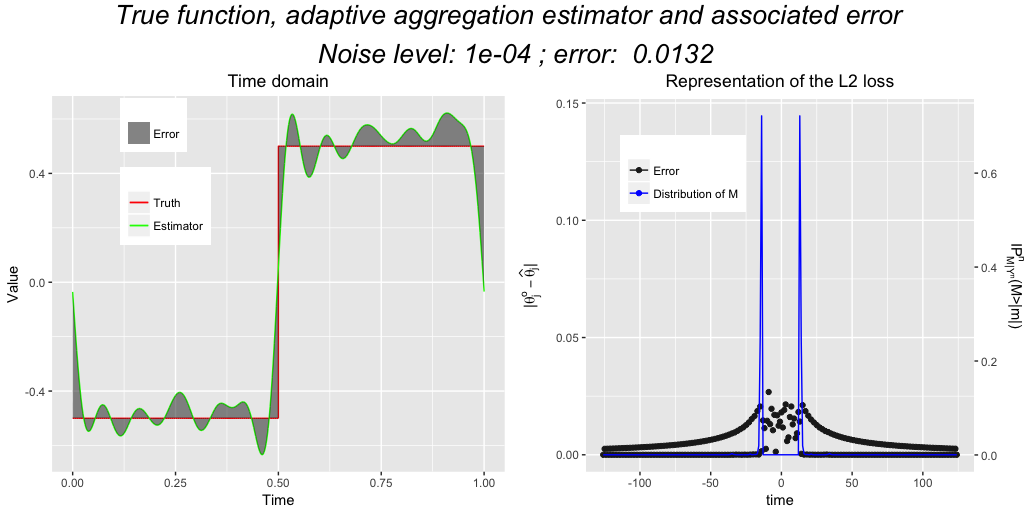
\includegraphics[width=.4\linewidth]{gauss/error/aggregation_error.png} \\[\abovecaptionskip]
  \end{tabular}
  \begin{tabular}{@{}c@{}}
    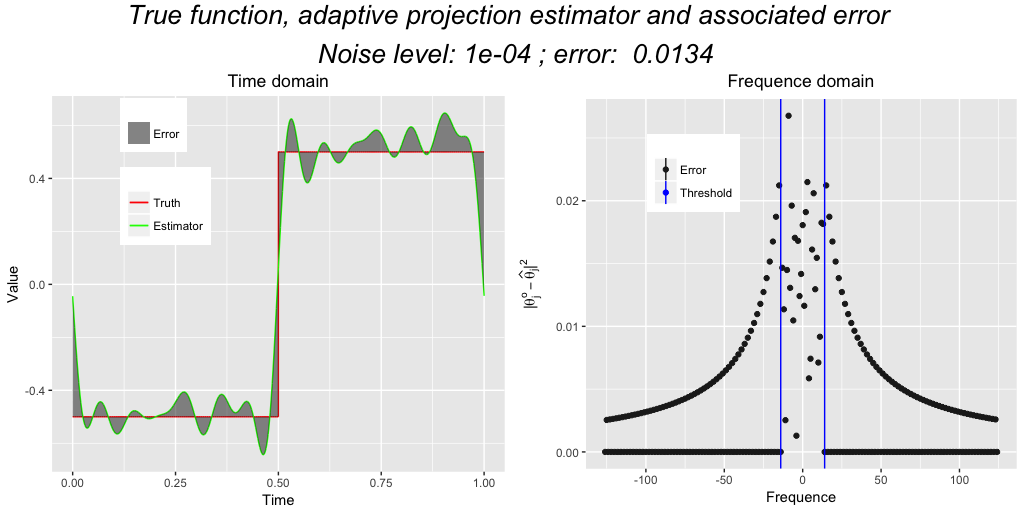
\includegraphics[width=.4\linewidth]{gauss/error/model_selection_error.png} \\[\abovecaptionskip]
  \end{tabular}
  \caption{Error of the aggregation estimator and of the model selection estimator for a fixed dataset}
  \label{fig:freq:igssm:error}
\end{figure}

Replicating the same experiment as in \nref{fig:freq:igssm:error} many times, it allows us to estimate the distribution of the error of each estimator at a fixed value of $n$, which we represent in \nref{fig:freq:igssm:error:mcmc}.

\begin{figure}
  \centering
  \begin{tabular}{@{}c@{}}
    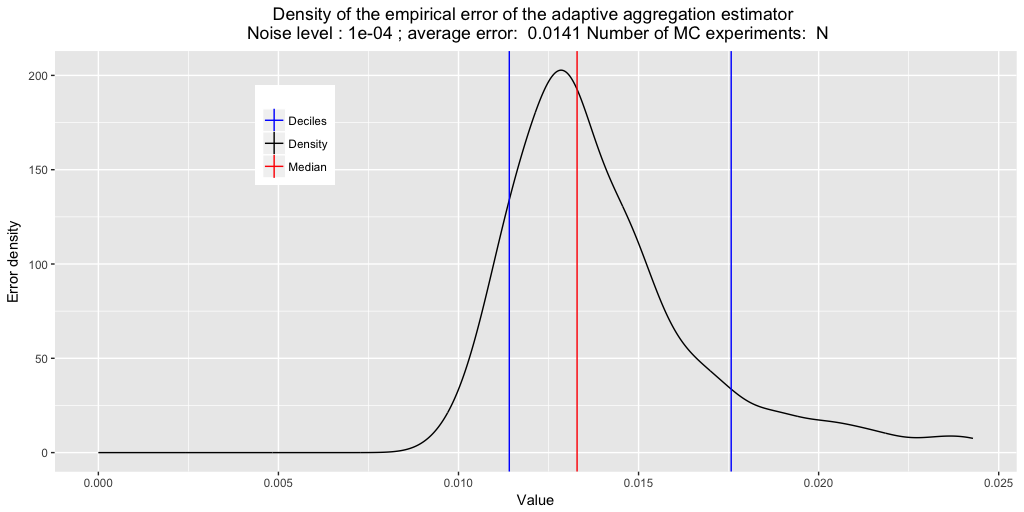
\includegraphics[width=.4\linewidth]{gauss/MCMC/error_aggregation.png} \\[\abovecaptionskip]
  \end{tabular}
  \begin{tabular}{@{}c@{}}
    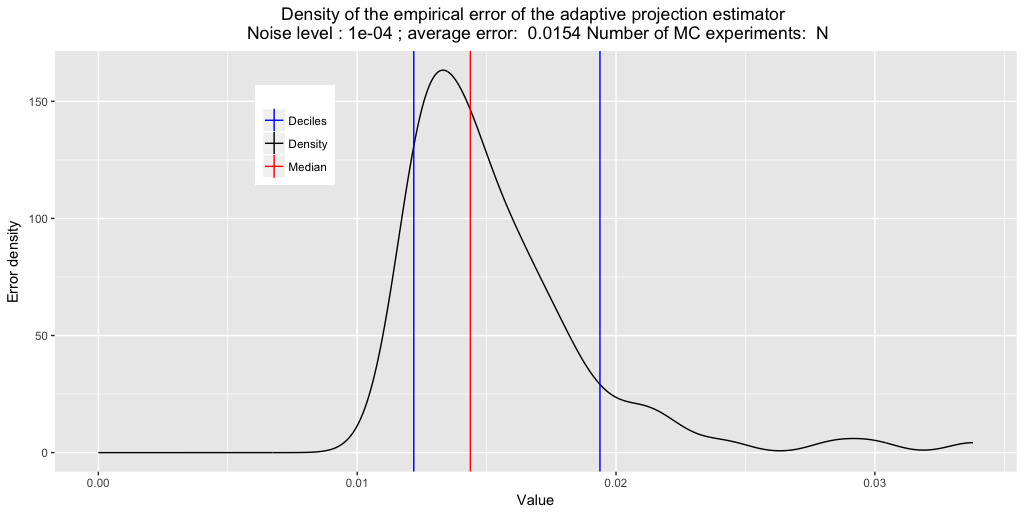
\includegraphics[width=.4\linewidth]{gauss/MCMC/error_model_selection.png} \\[\abovecaptionskip]
  \end{tabular}
  \caption{Kernel estimation of the density of the error for the aggregation estimator and the model selection estimator for a fixed true parameter $\theta^{\circ}$ and noise level $n$}
  \label{fig:freq:igssm:error:mcmc}
\end{figure}

Finally, replicating the experiment of \nref{fig:freq:igssm:error:mcmc} for different values of $n$ we can illustrate the evolution of the risk with $n$, as represented in \nref{fig:freq:igssm:error:evol}.

\begin{figure}
  \centering
  \begin{tabular}{@{}c@{}}
    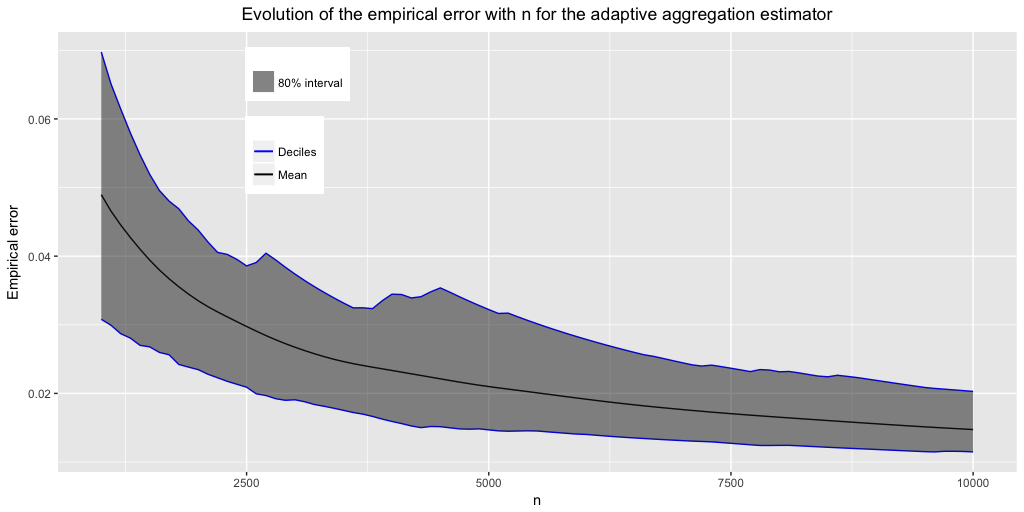
\includegraphics[width=.4\linewidth]{gauss/MCMC/evolution_error_aggregation.png} \\[\abovecaptionskip]
  \end{tabular}
  \begin{tabular}{@{}c@{}}
    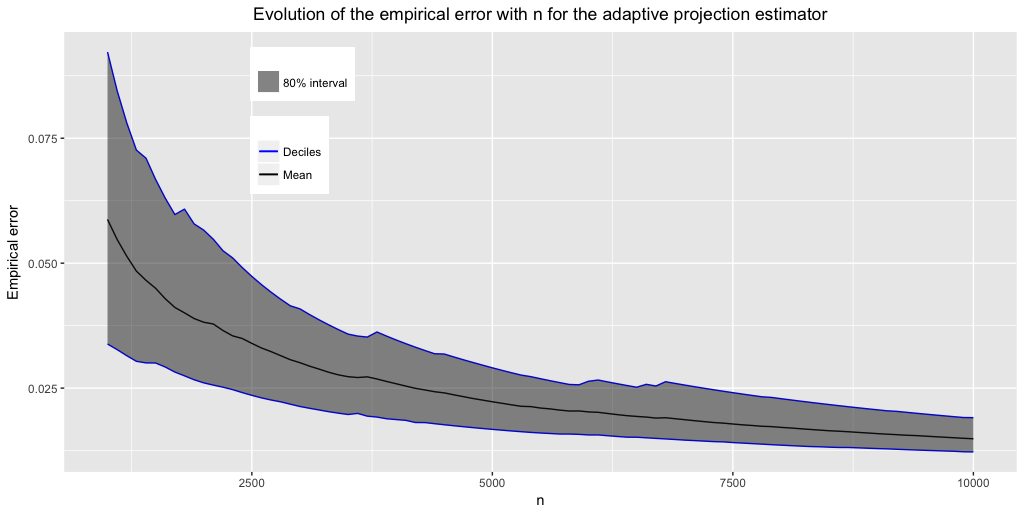
\includegraphics[width=.4\linewidth]{gauss/MCMC/evolution_error_model_selection.png} \\[\abovecaptionskip]
  \end{tabular}
  \caption{Estimation of the evolution with $n$ of the error of the aggregation estimator and of the model selection estimator}
  \label{fig:freq:igssm:error:evol}
\end{figure}

\subsubsection{Minimax optimality}
We now give interest to the maximal risk over Sobolev's ellipsoids.
We aim to apply \nref{ak:ag:ub:pnp:mm} which allows to show that the sequences defined hereafter are upper bounds for the maximal risk of our estimators.
\begin{de*}
  Let be the following family of sequences,
  $\daRa{\Di}{(\xdfCw[])}:=\daRa{\Di}{(\xdfCw[],\Lambda)}:=[\xdfCw^2\vee \DipenSv\,\ssY^{-1}]$.
Considering the following specific case, we aim to show that it describes an upper bound for the maximal risk over $\rwCxdf$ for our aggregation estimator,
    $\aDi{\ssY}(\xdfCw[]):=\argmin\Nset[\Di\in\Nz]{\daRa{\Di}{(\xdfCw[],\Lambda)}}\in\nset{1,\ssY}$\\
    $\naRa{(\xdfCw[])}:=\naRa{(\xdfCw[],\Lambda)}:=\min\Nset[\Di\in\Nz]{\daRa{\Di}{(\xdfCw[],\Lambda)}}$
    with $\daRa{\aDi{\ssY}(\xdfCw[])}{(\xdfCw[],\Lambda)}=\naRa{(\xdfCw[],\Lambda)}$
\assEnd
\end{de*}

The hypotheses to apply \nref{ak:ag:ub:pnp:mm} are the same as for \nref{freq:ge:strat:kn:qu:pnp} and hence we directly obtain the following result.

\begin{thm}
Assume that \nref{freq:ge:strat:kn:qu:as} holds true and consider the penalty sequence $\penSv:=\penD$, $\Di\in\nset{1,n}$, as in \nref{freq:ge:shape:kn:de:pen:oo}.
Let $\txdfAg[{\erWe[]}]=\sum_{\Di=1}^{\ssY} \We\txdfPr$ be an aggregation of the orthogonal series estimators using either aggregation weights $\rWe[]$ as in \eqref{freq:ge:shape:kn:we} or model selection weights $\msWe[]$ as in \eqref{freq:ge:shape:uk:we}. % Let $\Di_{\edf,\xdfCr}:=\floor{3(800\Vnorm[{\xdfCw[]}]{\edf}\xdfCr)^2}$ and
    % $ \ssY_{o}:=15({300})^4$.
There is a finite constant $\cst{\xdfCw[],\xdfCr,\Lambda}$ given in
\eqref{ak:ag:ub:pnp:p8} depending only on $\xdfCw[]$, $\xdfCr$ and $\Lambda$ such that for all
$\ssY\in\Nz$ and for all $\sDi{\ssY}\in\nset{\aDi{\ssY}(\xdfCw[]),\ssY}$  with
 $\aDi{\ssY}(\xdfCw[])\in\nset{1,n}$ as in \nref{freq:ge:strat:kn:ma:de:rate} holds 
 \begin{equation}
 \nRi{\txdfAg[{\erWe[]}]}{\rwCxdf,\Lambda}
   %\sup_{\xdf\in\rwCxdf}\E\Vnormlp{\txdfAg[{\erWe[]}]-\xdf}^2% \leq
    \leq 
   \cst{}(\xdfCr^2\vee1)\min_{\Di\in\nset{1,\ssY}}\big[\daRa{\Di}{(\xdfCw[],\Lambda)}\vee\exp\big(-2\cmiSv\Di\big)]\big)\big]
   +\cst{\xdfCw[],\xdfCr,\Lambda}\ssY^{-1}.
\end{equation}
\reEnd
\end{thm}

\begin{cor}
  Let the assumptions of \nref{ak:ag:ub:pnp:mm} be satisfied.  If in
  addition
  \begin{inparaenum}\item[{{\dgrau\bfseries(A)}}]
    there is $\ssY_{\xdfCw[],\xdfCr,\Lambda}\in\Nz$  such that
    $\aDi{\ssY}({\xdfCw[]})\cmSv[\aDi{\ssY}({\xdfCw[]})]\geq \vert \log\naRa{(\xdfCw[])} \vert/2 $
    for all $\ssY\geq \ssY_{\xdfCw[],\xdfCr,\Lambda}$
  \end{inparaenum}
  holds true, then there is a constant $\cst{\xdfCw[],\xdfCr,\Lambda}$
  depending only on $\rwCxdf$ and $\Lambda$ such that
  $ \nRi{\txdfAg[{\erWe[]}]}{\rwCxdf,\Lambda} \leq
  \cst{\xdfCw[],\xdfCr,\Lambda}\naRa{(\xdfCw[],\Lambda)}$ for all $n\in\Nz$
  holds true.
  \reEnd
\end{cor}


\subsection{Unknown operator}\label{freq:igssm:uk}
We now consider the case when $\lambda$ is unknown and we hence use the observations $(\epsilon_{p})_{p \in \llbracket 1, n_{\lambda} \rrbracket}$ to estimate it.
\subsubsection{Shape of the estimator}
\begin{de*}
We use, as usual an aggregation estimator, where, this time, the aggregating sequence does not depend on $\lambda$ but on $\epsilon^{n_{\lambda}}$,
\begin{equation*}
(\widehat{\theta}^{(\eta)}(s))_{s \in \mathds{F}} = (\sum\nolimits_{m \in \N} \widehat{\P}_{M}^{(\eta)} \cdot \theta_{n, n_{\lambda}, \overline{m}}(s))_{s \in \mathds{F}} = (\sum\nolimits_{m \geq \vert s \vert} \widehat{\P}_{M}^{(\eta)} \cdot \theta_{n, n_{\lambda}}(s))_{s \in \mathds{F}}.
\end{equation*}
In particular, we give the following shape to the aggregating sequence with the contrast $\Upsilon$ and penalty $\pen^{\widehat{\Lambda}}$,
\begin{multline*}
\Upsilon : \N \to \R_{+}, \quad m \mapsto \Upsilon(m); \qquad \pen^{\widehat{\Lambda}} : \N \to \R_{-}, \quad m \mapsto \pen^{\widehat{\Lambda}}(m);\\
\widehat{\P}_{M}^{(\eta)} : \N \to \R_{+}; \quad m \mapsto \tfrac{\exp[\eta n (\Upsilon(m) + \pen^{\widehat{\Lambda}}(m))]}{\sum\nolimits_{k = 0}^{n} \exp[\eta n (\Upsilon(k) + \pen^{\widehat{\Lambda}}(k))]} \mathds{1}_{m \leq n}.
\end{multline*}
Notice that if we let $\eta$ tend to infinity we obtain the following penalised contrast model selection estimator,
\begin{equation*}
  \hDi:=\argmin_{\Di\in\nset{1,\ssY}} \big\{\Upsilon(m)+\peneSv\big\}
\end{equation*}
which corresponds to the following weight sequence,
\begin{equation*}
  \lim_{\rWc\to\infty}\erWe=\dirac[\hDi](\{\Di\})=:\widehat{\P}_{M}^{(\infty)}.
\end{equation*}
In particular, we take the following expressions for $\Upsilon$ and $\pen^{\widehat{\Lambda}}$, with $\kappa := 84$,
\begin{alignat*}{4}
  & \Upsilon(m) && := && \Vert \theta_{n, n_{\lambda}, \overline{m}}\Vert_{l^{2}}^{2}; && \quad \eiSv[(s)]:= \vert \hfedfmpI[(s)] \vert ^2\\
    & \meiSv && := && \max\{\eiSv[(l)],l\in\nset{1,\Di}\}; && \quad \cmeiSv:=\tfrac{\log^{2}(\Di\meiSv\vee(\Di+2))}{\log^{2}(\Di+2)}\geq1;\\
    &\DipeneSv && := && \cmeiSv \Di \meiSv;&& \quad \peneSv:= \peneD.
  \end{alignat*}
\assEnd
\end{de*}

\subsubsection{Oracle optimality}
We first look at the quadratic risk for each $\theta^{\circ}$ and we recall the sequence which shall be an upper bound for the quadratic risk of our estimators.
\begin{de*}
Remind that we defined for any $\theta$ in $\Theta$ and $\Di$ in $\N$ the following term $\b_{m}^{2}(\theta) = \Vert \theta_{\underline{m}} \Vert_{l^{2}}/\Vert \theta_{\underline{0}} \Vert_{l^{2}} \leq 1$.
We then define a family of sequences $(\daRa{\Di}{(\xdf)})_{\Di \in \N} := (\daRa{\Di}{(\xdf,\Lambda)})_{\Di \in \N} = [\b_{m}^{2}(\theta^{\circ}) \vee \penSv/\cpen]$.
We intend to prove that the specific choice
\begin{multline*}
\aDi{\ssY}(\xdf):=\argmin\Nset[\Di\in\Nz]{\daRa{\Di}{(\xdf)}}\in\nset{1,\ssY}; \\
\naRa{(\xdf)}:=\naRa{(\xdf,\Lambda)}:=\min\Nset[\Di\in\Nz]{\daRa{\Di}{(\xdf)}}
\end{multline*}
with $\daRa{\aDi{\ssY}}{(\xdf,\Lambda)}=\naRa{(\xdf,\Lambda)}$ defines an upper bound for the convergence rate of the aggregation estimators.
\assEnd
\end{de*}
Our method gives us a simple assumption to verify in order to obtain this result.

The following result, which is a direct application, once again, of \nref{lmA.1.1} and \nref{lmA.1.2} gives us precisely what we want.
\begin{cor*}
For any $m$, $\ssY$, and $\ssE$ in $\N$ we have,
\begin{alignat*}{3}
& \E_{\phi_{n} \vert \lambda_{n_{\lambda}}}[(\Vert \theta_{n, n_{\lambda}, \overline{m}} - \dxdfPr \Vert_{l^{2}}^{2} - 12 \Delta_{\widehat{\Lambda}}(m) n ^{-1})_{+}] && \leq && 6 n^{-1} \widehat{\Lambda}_{+}(m) \exp[- 2 \delta_{\widehat{\Lambda}}(m)];\\
& \P_{\phi_{n} \vert \lambda_{n_{\lambda}}}[\Vert \theta_{n, n_{\lambda}, \overline{m}} - \dxdfPr \Vert_{l^{2}}^{2} \geq 12 \Delta_{\widehat{\Lambda}}(m) n ^{-1}] && \leq && \exp[- 2 \delta_{\widehat{\Lambda}}(m)];\\
& \P(\vert \lambda_{n_{\lambda}}(s)/\lambda(s) - 1 \vert > 1/3) && \leq && \exp[-\tfrac{n_{\lambda}}{6 \Lambda(s)}].
\end{alignat*}
\reEnd
\end{cor*}

The following theorem is then a direct consequence of \nref{au:ag:ub:pnp} and we omit its proof.
\begin{thm}
Consider the   penalty sequence $\peneSv:=\peneD$,
  $\Di\in\nset{1,\ssY}$, as in \nref{freq:ge:shape:uk:de:pen:oo}.
  Let $\hxdfAg[{\erWe[]}]=\sum_{\Di=1}^{\ssY} \erWe\hxdfPr$ be an aggregation of the orthogonal series estimators using either aggregation weights $\erWe[]$ as in \eqref{freq:ge:shape:uk:we} or model selection weights $\msWe[]$ as in \nref{freq:ge:shape:uk:de:msWe}.
  \begin{Liste}[]
  \item[{\dgrau\bfseries{(p)}}]Assume there is
    $K\in\Nz_0$ with $1\geq \bias[{[K-1] }](\xdf)>0$ and
    $\bias[\Di](\xdf)=0$. For $K>0$ let
    $c_{\xdf}:=\tfrac{\Vnormlp{\xdf_{\underline{0}}}^2+104\cpen}{\Vnormlp{\xdf_{\underline{0}}}^2\bias[{[K-1]}]^2(\xdf)}>1$,
    $\ssY_{\xdf,\Lambda}:=\floor{c_{\xdf}\DipenSv[K]}\in\Nz$ and
    $\ssE(\xdf,\Lambda):=\floor{289\log(K+2)\cmiSv[K]\miSv[K]}\in\Nz$. If
    $\ssY>\ssY_{\xdf,\Lambda}$ and $\ssE>\ssE(\xdf,\Lambda)$ then set
    $\sDi{\ssY}:=\max\{\Di\in\nset{K,\ssY}:\ssY>c_{\xdf}\DipenSv\}$
    and
    $\sDi{\ssE}:=\max\{\Di\in\nset{K,\ssE}:289\log(\Di+2)\cmiSv[\Di]\miSv[\Di]\leq\ssE\}$
    where the defining set, respectively, contains $K$ and thus is not
    empty, and otherwise $\sDi{\ssY}\wedge\sDi{\ssE}:=\Di_{\cst{3}}\log(\ssY\wedge\ssE)$.
    There is a numerical constant $\cst{}$ and a  constant $\cst{\xdf,\Lambda}$ given in
    \eqref{au:ag:ub:pnp:p9} depending only on $\xdf$ and $\Lambda$ such
    that for all $\ssY,\ssE\in\Nz$ holds
    \begin{equation}
       \nmRi{\hxdfAg[{\erWe[]}]}{\xdf,\Lambda}
       %\E\Vnormlp{\widehat{\theta}^{(\eta)}-\xdf}^2
       \leq
      \cst{}\Vnormlp{\xdf_{\underline{0}}}^2\big[\ssY^{-1}\vee \ssE^{-1} \vee
      \exp\big(\tfrac{-\cmiSv[\sDi{\ssY}\wedge\sDi{\ssE}]\sDi{\ssY}\wedge\sDi{\ssE}}{\Di_{\cst{3}}}\big)\big]\\
      + \cst{\xdf,\Lambda}\{\ssY^{-1}\vee\ssE^{-1}\}.
    \end{equation}
  \item[{\dgrau\bfseries{(np)}}] Assume that
    $\bias(\xdf)>0$ for all $\Di\in\Nz$. Let    
    $\ssE(\Lambda):=\floor{289\log(3)\cmiSv[1]\miSv[1]}\in\Nz$. If
    $\ssE>\ssE(\Lambda)$ then set
    $\sDi{\ssE}:=\max\{\Di\in\nset{1,\ssE}:289\log(\Di+2)\cmiSv[\Di]\miSv[\Di]\leq\ssE\}$
    where the defining set, respectively, contains $1$ and thus is not
    empty.  There is a numerical constant $\cst{}$  such that for all $\ssY\in\Nz$
    with $\aDi{\ssY}:=\aDi{\ssY}(\xdf)\in\nset{1,n}$ as in \nref{freq:ge:strat:kn:ma:de:rate} and
    for all $\ssE>\ssE(\Lambda)$ holds
    \begin{multline}
     \nmRi{\hxdfAg[{\erWe[]}]}{\xdf,\Lambda}  
     %\E\Vnormlp{\widehat{\theta}^{(\eta)}-\xdf}^2
     \leq\cst{}(1\vee\Vnormlp{\xdf_{\underline{0}}}^2)\min_{\Di\in\nset{1,\ssY}}\{\daRa{\Di}{(\xdf,\Lambda)}\vee\exp\big(\tfrac{-\cmiSv[\Di]\Di}{\Di_{\cst{3}}}\big)\}\Ind{\{\ssE>\ssE(\Lambda)\}}\\\hfill
+\cst{}(1\vee\Vnormlp{\xdf_{\underline{0}}}^2)\{\bias[\aDi{\ssY}\wedge\sDi{\ssE}]^2(\xdf)\vee\exp\big(\tfrac{-\cmiSv[\sDi{\ssE}]\sDi{\ssE}}{\Di_{\cst{3}}}\big)\}\Ind{\{\ssE>\ssE(\Lambda)\}} \\\hfill
 +\cst{}\mRa{\xdf,\Lambda}   + \cst{}(1\vee\Vnormlp{\xdf_{\underline{0}}}^2)\miSv[1]^2\ssE^{-1}  
    +\cst{}\{\miSv[\Di_{\cst{3}}]^2\Di_{\cst{3}}^3+\miSv[\ssY_{o}]^2\}\ssY^{-1}
  \end{multline}
  while for $\ssE\in\nset{1,\ssE(\Lambda)}$ we have
  
  $\cst{}\mRa{\xdf,\Lambda}
    + \cst{}(1\vee\Vnormlp{\xdf_{\underline{0}}}^2)\miSv[1]^2\ssE^{-1}  
    +\cst{}\{\miSv[\Di_{\cst{3}}]^2\Di_{\cst{3}}^3+\miSv[\ssY_{o}]^2\}\ssY^{-1}$. 
\end{Liste}  
\reEnd
\end{thm}

\begin{cor}
  \begin{Liste}[]
  \item[{\dgrau\bfseries{(p)}}]
    If \ref{ge:ak:ag:ub2:pnp:pc} as in \nref{ge:ak:ag:ub2:pnp} and 
    in addition
    \begin{inparaenum}% \item[\mylabel{ge:au:ag:ub2:pnp:pc:a}{{\dgrau\bfseries(A1)}}]
      % there is $\ssY_{\xdf,\Lambda}\in\Nz$ such that
      % $\cmiSv[\sDi{\ssY}]\sDi{\ssY}\geq \Di_{\cst{3}}(\log\ssY)$ for all
      % $\ssY\geq \ssY_{\xdf,\Lambda}$ and
    \item[{{\dgrau\bfseries(A4)}}]
            there is
            
            $\ssE(\xdf,\Lambda)\in\Nz$ such that
      $\cmiSv[\sDi{\ssE}]\sDi{\ssE}\geq \Di_{\cst{3}}(\log\ssE)$ for all
      $\ssE\geq \ssE(\xdf,\Lambda)$ 
    \end{inparaenum}
    hold true, then there is a constant $\cst{\xdf,\Lambda}$ depending
    only on $\xdf$ and $\Lambda$ such that for all $\ssY,\ssE\in\Nz$ holds
    $\nmRi{\hxdfAg[{\erWe[]}]}{\xdf,\Lambda} \leq
    \cst{\xdf,\Lambda}[\ssY^{-1}\vee\ssE^{-1}]$.
  \item[{\dgrau\bfseries{(np)}}]
    If  \ref{ge:ak:ag:ub2:pnp:npc} as in \nref{ge:ak:ag:ub2:pnp} and \ref{ge:au:ag:ub2:pnp:pc:b}
    hold true, then there is a constant $\cst{\xdf,\Lambda}$ depending
    only on $\xdf$ and $\Lambda$ such that $\nmRi{\hxdfAg[{\erWe[]}]}{\xdf,\Lambda}
    \leq \cst{\xdf,\Lambda}\{\naRa{(\xdf,\Lambda)}+\mRa{\xdf,\Lambda}+\bias[\sDi{\ssE}\wedge\aDi{\ssY}]^2(\xdf)\}$ for all $\ssY,\ssE\in\Nz$ holds true.
  \end{Liste}  
\end{cor}
\subsubsection{Minimax optimality}
We now give interest to the maximal risk over Sobolev's ellipsoids.
We aim to apply \nref{ak:ag:ub:pnp:mm} which allows to show that the sequences defined hereafter are upper bounds for the maximal risk of our estimators.
\begin{de*}
  Let be the following family of sequences,
  $\daRa{\Di}{(\xdfCw[])}:=\daRa{\Di}{(\xdfCw[],\Lambda)}:=[\xdfCw^2\vee \DipenSv\,\ssY^{-1}]$.
Considering the following specific case, we aim to show that it describes an upper bound for the maximal risk over $\rwCxdf$ for our aggregation estimator,
    $\aDi{\ssY}(\xdfCw[]):=\argmin\Nset[\Di\in\Nz]{\daRa{\Di}{(\xdfCw[],\Lambda)}}\in\nset{1,\ssY}$\\
    $\naRa{(\xdfCw[])}:=\naRa{(\xdfCw[],\Lambda)}:=\min\Nset[\Di\in\Nz]{\daRa{\Di}{(\xdfCw[],\Lambda)}}$
    with $\daRa{\aDi{\ssY}(\xdfCw[])}{(\xdfCw[],\Lambda)}=\naRa{(\xdfCw[],\Lambda)}$
\assEnd
\end{de*}

The hypotheses to apply \nref{ak:ag:ub:pnp:mm} are the same as for \nref{freq:ge:strat:kn:qu:pnp} and hence we directly obtain the following result.

\begin{thm}
  Consider the   penalty sequence $\peneSv:=\peneD$,
  $\Di\in\nset{1,\ssY}$, as in \nref{freq:ge:shape:uk:de:pen:oo} with numerical
  constant $\cpen\geq84$. Let
  $\hxdfAg[{\erWe[]}]=\sum_{\Di=1}^{\ssY} \erWe\hxdfPr$ be an
  aggregation of the orthogonal series estimators using either
  aggregation weights $\erWe[]$ as in \eqref{freq:ge:shape:uk:we} or model
  selection weights $\msWe[]$ as in \nref{freq:ge:shape:uk:de:msWe}. Let
  $\dr\Di_{\edf,\xdfCr}:=\floor{3(400\Vnorm[{\xdfCw[]}]{\edf}\xdfCr)^2}$
  and $\dr \ssY_{o}:=15({600})^4$. Let
  $\ssE(\Lambda):=\floor{289\log(3)\cmiSv[1]\miSv[1]}\in\Nz$. If
  $\ssE>\ssE(\Lambda)$ then set
  $\sDi{\ssE}:=\max\{\Di\in\nset{1,\ssE}:289\log(\Di+2)\cmiSv[\Di]\miSv[\Di]\leq\ssE\}$
  where the defining set, respectively, contains $1$ and thus is not
  empty.  There is a numerical constant $\cst{}$ such that for all
  $\ssY\in\Nz$ with $\aDi{\ssY}:=\aDi{\ssY}(\xdf)\in\nset{1,n}$ as in
  \nref{freq:ge:shape:uk:de:pen:oo} and for all $\ssE>\ssE(\Lambda)$ holds
  \begin{multline}
    \nmRi{\hxdfAg[{\erWe[]}]}{\rwCxdf,\Lambda}  
    \leq\cst{}(1\vee\xdfCr^2)\min_{\Di\in\nset{1,\ssY}}
    \{\daRa{\Di}{(\xdfCw[],\Lambda)}\vee
    \exp\big(\tfrac{-\cmiSv[\Di]\Di}{\Di_{\edf,\xdfCr}}\big)\} \\\hfill
    +\cst{}(1\vee\xdfCr^2)\{\xdfCw[(\aDi{\ssY}\wedge\sDi{\ssE})]^2\vee
    \exp\big(\tfrac{-\cmiSv[\sDi{\ssE}]\sDi{\ssE}}{\Di_{\edf,\xdfCr}}\big)\}\\\hfill
    +\cst{}\xdfCr^2\mmRa{\xdfCw[],\Lambda}   + \cst{}(1\vee\xdfCr^2)\miSv[1]^2\ssE^{-1}  
    +\cst{}\{\miSv[\Di_{\edf,\xdfCr}]^2\Di_{\edf,\xdfCr}^3+\miSv[\ssY_{o}]^2\}\ssY^{-1}
  \end{multline}
  while for $\ssE\in\nset{1,\ssE(\Lambda)}$ we have
  \begin{multline}
    \nmRi{\hxdfAg[{\erWe[]}]}{\rwCxdf,\Lambda}  
    \leq \cst{}\xdfCr^2\mmRa{\xdfCw[],\Lambda}
    + \cst{}(1\vee\xdfCr^2)\miSv[1]^2\ssE^{-1}\\
    +\cst{}\{\miSv[\Di_{\edf,\xdfCr}]^2\Di_{\edf,\xdfCr}^3+\miSv[\ssY_{o}]^2\}\ssY^{-1}.
  \end{multline}
\end{thm}


\begin{cor}
  Let the assumptions of \nref{au:mrb:ag:ub:pnp} be satisfied.
    If  \ref{ge:ak:ag:ub2:pnp:npc} as in \nref{ge:ak:ag:ub2:pnp} and \ref{ge:au:ag:ub2:pnp:pc:b}
    as in \nref{ge:au:ag:ub2:pnp} hold true, then there is a constant $\cst{\xdfCw[],\xdfCr,\Lambda}$ depending
    only on $\xdfCw[]$, $\xdfCr$ and $\Lambda$ such that $\nmRi{\hxdfAg[{\erWe[]}]}{\rwCxdf,\Lambda}
    \leq \cst{\xdfCw[],\xdfCr,\Lambda}\{\naRa{(\xdfCw[],\Lambda)}+\mmRa{\xdfCw[],\Lambda}+\xdfCw[(\sDi{\ssE}\wedge\aDi{\ssY})]^2\}$ for all $\ssY,\ssE\in\Nz$ holds true.
\end{cor}
%%
\section{Circular deconvolution model}\label{FREQ_CIRCULARDECONVOLUTION}
We place ourselves in the framework introduced in \nref{INTRO_CIRCULARDECONVOLUTION}.
We will first consider the case of a known operator, first with independent data, then with an absolutely regular process.
We will then consider an unknown operator.
In all cases, we start by giving the explicit, detailed expression of the estimator, as well as the sequence which shall be proven o be an upper bound for the quadratic risk, before reminding the hypotheses to prove in order to obtain the convergence, we shall then proceed to show that the said hypothesis holds true before concluding.
The proofs for the results obtained in this section may be found in \nref{a:prel}.


 %======================================================================================================================
%                                                                 
% Title:  Aggregated CDE: known error density
% Author: Jan JOHANNES, Institut für Angewandte Mathematik, Ruprecht-Karls Universität Heidelberg, Deutschland  
% 
% Email: johannes@math.uni-heidelberg.de
% Date: %%ts latex start%%[2018-03-29 Thu 12:11]%%ts latex end%%
%
% ======================================================================================================================
% --------------------------------------------------------------------
% section <<Aggregated CDE: known error density>>\nref{ak}
% --------------------------------------------------------------------
\subsection{Independent data and known convolution density}\label{FREQ_DECONV_KNOWN}\label{ak:rb}\label{AK:RB}
% ....................................................................
% <<Text Aggregated CDE>>
% ....................................................................
\begin{te}
We place ourselves under \nref{AS_INTRO_DATA_KNOWN} and \nref{AS_INTRO_DATA_INDEPENDENT} and intend to apply the strategy highlighted in \nref{freq:ge:strat:kn}.
\end{te}

We assume here that we know $\lambda$ and observe the vector of independent random variables $Y^{n}$.
Assume now that for any $s$ in $\N$, we know $\lambda(s)$ and $\lambda(s) > 0$.
\subsubsection{Shape of the estimator}
First, let us remind that we plan to use an aggregated orthogonal series estimator $\widehat{\theta}^{(\eta)}$, with $\eta$ in $\R_{+}^{\star} \cup \infty$ which form is reminded hereafter.
\begin{de*}
We first define so-called contrast $\Upsilon$ and penalisation $\pen^{\Lambda}$ sequences, which allow us to define weight $\P_{M}^{(\eta)}$ on the nested sieve space (here $(\llbracket 0, m \rrbracket)_{m \in \N}$)
\begin{multline*}
\Upsilon : \mathds{N} \to \R_{+}, \quad m \mapsto \Upsilon(m); \qquad \pen^{\Lambda} : \N \to \R_{-}, \quad m \mapsto \pen^{\Lambda}(m);\\
\P_{M}^{(\eta)} : \N \to \R_{+}, \quad m \mapsto \tfrac{\exp[\eta n (\Upsilon(m) + \pen^{\Lambda}(m))]}{\sum\nolimits_{k = 0}^{n} \exp[\eta n (\Upsilon(k) + \pen^{\Lambda}(k))]} \mathds{1}_{m \leq n}.
\end{multline*}
Notice that letting $\eta$ tend to $\infty$ in the previous definition gives rise to the penalised contrast model selection estimator,
\begin{equation*}
  \tDi:=\argmin\nolimits_{\Di\in\nset{1,\ssY}} \big\{\Upsilon(m) + \penSv\big\}
\end{equation*}
which corresponds to the following weights
\begin{equation*}
  \lim\nolimits_{\rWc\to\infty}\rWe=\dirac[\tDi](\{\Di\})=:\msWe.
\end{equation*}
Here, we will use the following shape for $\Upsilon$ and $\pen^{\Lambda}$, for $\cpen := 84$
\begin{alignat*}{4}
  & \Upsilon(m) && := && \Vert \theta_{n, \overline{m}} \Vert_{l^{2}}^{2};  \quad && \cmiSv := \tfrac{\log^{2}(\Di\miSv \vee(\Di+2))}{\log^{2}(\Di+2)}\geq1;\\
  & \DipenSv && := && \cmiSv \Di \miSv; \quad && \penSv:= \penD.
  \end{alignat*}
  \assEnd
\end{de*}
The family of estimators is hence entirely defined and can be implemented with the data we assume to have at hand in this subsection.
  
 \subsubsection{Quadratic risk bounds of the aggregated estimator}\label{AK:RB:OR}
 In a first time we are interested in the quadratic risk for any $\theta^{\circ}$ fixed.
Remind that the strategy we use allows to show that the following sequence is an upper bound for the quadratic risk.
\begin{de*}
Remind that we defined for any $\theta$ in $\Theta$ and $\Di$ in $\N$ the following term $\b_{m}^{2}(\theta) = \Vert \theta_{\underline{m}} \Vert_{l^{2}}/\Vert \theta_{\underline{0}} \Vert_{l^{2}} \leq 1$.
We then define a family of sequences $(\daRa{\Di}{(\xdf)})_{\Di \in \N} := (\daRa{\Di}{(\xdf,\Lambda)})_{\Di \in \N} = [\b_{m}^{2}(\theta^{\circ}) \vee \penSv/\cpen]$ and hence it holds for all $\Di$ in $\nset{1,\ssY}$
    \begin{equation}
      [\Vnormlp{\xdf_{\underline{0}}}^2+\cpen]\daRa{\Di}{(\xdf)}\geq\Vnormlp{\xdf_{\underline{0}}}^2\bias^2(\xdf)\vee\penSv.
      \end{equation}
We intend to prove that the specific choice
\begin{multline*}
\aDi{\ssY}(\xdf):=\argmin\Nset[\Di\in\Nz]{\daRa{\Di}{(\xdf)}}\in\nset{1,\ssY}; \\
\naRa{(\xdf)}:=\naRa{(\xdf,\Lambda)}:=\min\Nset[\Di\in\Nz]{\daRa{\Di}{(\xdf)}}
\end{multline*}
with $\daRa{\aDi{\ssY}}{(\xdf,\Lambda)}=\naRa{(\xdf,\Lambda)}$ defines an upper bound for the convergence rate of the aggregation estimators.
\assEnd
\end{de*}
 
The following lemma shows that the assumption for our method is verified.
\begin{lm}\label{re:conc}
  Let $\oiSv=\tfrac{1}{\Di}\sum_{s\in\nset{1,\Di}}\iSv[s]$,
  $\miSv= \max\{\iSv[s],s\in\nset{1,\Di}\}$, $\cmSv\geq1$ and
  $\DipenSv=\cmSv\Di \miSv$, then there is a numerical constant
  $\cst{}$ such that for all $\ssY\in\Nz$ and
  $\Di\in\nset{1,\ssY}$ holds
  \begin{resListeN}[]
  \item\label{re:conc:i}
    $\E \vectp{\Vnormlp{\txdfPr-\xdfPr}^2 - 12\DipenSv\ssY^{-1}}\\
    \leq 
    \cst{} \bigg[\tfrac{\Vnormlp[1]{\fydf}\,\miSv}{\ssY}\exp\big(\tfrac{-\cmSv\Di}{3\Vnormlp[1]{\fydf}}\big)+\tfrac{2\Di\miSv}{n^2}\exp\big(\tfrac{-\sqrt{n\cmSv}}{200}\big) \bigg]$
  \item\label{re:conc:ii}
    $\P\big(\Vnormlp{\txdfPr-\xdfPr}^2 \geq 12\DipenSv\ssY^{-1}\big)\leq 
    3 \bigg[\exp\big(\tfrac{-\cmSv\Di}{200\Vnormlp[1]{\fydf}}\big)
    +\exp\big(\tfrac{-\sqrt{\ssY\cmSv}}{200}\big)\bigg]$
  \item\label{re:conc:iii}
    $\P\big(\Vnormlp{\txdfPr-\xdfPr}^2 \geq 12\daRa{\Di}{(\xdf,\Lambda)}\big)\leq 
    3 \bigg[\exp\big(\tfrac{-\ssY\daRa{\Di}{(\xdf,\Lambda)}}{200\Vnormlp[1]{\fydf}\miSv}\big)
    +\exp\big(\tfrac{-\ssY\sqrt{\daRa{\Di}{(\xdf,\Lambda)}}}{200\sqrt{\Di\miSv}}\big)\bigg]$
  \end{resListeN}
\end{lm}

Hence, using \nref{freq:ge:strat:kn:qu:pnp} gives us the following result.
% ....................................................................
% <<Re upper bound ag p np>>
% ....................................................................
\begin{thm}
Consider the penalty sequence $\penSv:=\penD$, $\Di\in\nset{1,n}$, as in \nref{freq:ge:shape:kn:de:pen:oo} with numerical constant $\cpen \geq 84$.
Let $\txdfAg[{\erWe[]}]=\sum_{\Di=1}^{\ssY}\We\txdfPr$ be an aggregation of the orthogonal series estimators, using either aggregation weights $\rWe[]$ as in \eqref{freq:ge:shape:kn:we}, or model selection weights $\msWe[]$ as in \eqref{freq:ge:shape:kn:de:msWe}.
\begin{Liste}[]
\item[{\dgrau\bfseries{(p)}}]Assume there is $K\in\Nz$
  with   $1\geq \bias[{[K-1] }](\xdf)>0$ and $\bias[\Di](\xdf)=0$. For
  $K>0$ let
  $ c_{\xdf}:=\tfrac{\Vnormlp{\xdf_{\underline{0}}}^2+4\cpen}{\Vnormlp{\xdf_{\underline{0}}}^2\bias[{[K-1]}]^2(\xdf)}>1$ and
  $\ssY_{\xdf}:=\gauss{c_{\xdf}\DipenSv[K]}\in\Nz$. If
  $\ssY\in\nset{1,\ssY_{\xdf}}$ then set $\sDi{\ssY}:=\Di_{\cst{3}}\log(\ssY)$, and otherwise if
  $\ssY>\ssY_{\xdf}$ then set
  $\sDi{\ssY}:=\max\{\Di\in\nset{K,\ssY}:\ssY>c_{\xdf}\DipenSv\}$
  where the defining set contains $K$ and thus is not empty.
There is a finite constant $\cst{\xdf,\Lambda}$
given in \eqref{ak:ag:ub:pnp:p7} depending only on $\xdf$ and $\Lambda$ such that for all $n\in\Nz$ holds
\begin{equation}
  \nRi{\txdfAg[{\erWe[]}]}{\xdf,\Lambda}
  % \E\Vnormlp{\txdfAg[{\erWe[]}]-\xdf}^2
  \leq
  \cst{}\Vnormlp{\xdf_{\underline{0}}}^2\big[
  \ssY^{-1}\vee\exp\big(-2\cmiSv[\sDi{\ssY}]\sDi{\ssY}\big)\big]
  + \cst{\xdf,\Lambda}\ssY^{-1}.
\end{equation}
\item[{\dgrau\bfseries{(np)}}] Assume that
  $\bias(\xdf)>0$ for all  $\Di\in\Nz$.
There is a finite finite constant $\cst{\xdf,\Lambda}$ given in
\eqref{ak:ag:ub:pnp:p8} depending only $\xdf$ and $\Lambda$ such that for all
$\ssY\in\Nz$  holds 
 \begin{equation}
   \nRi{\txdfAg[{\erWe[]}]}{\xdf,\Lambda}
   % \E\Vnormlp{\txdfAg[{\erWe[]}]-\xdf}^2
    \leq 
   \cst{}(\Vnormlp{\xdf_{\underline{0}}}^2\vee1)\min_{\Di\in\nset{1,\ssY}}\big[\dRa{\Di}{\xdf,\Lambda}\vee\exp\big(-2\cmiSv\Di\big)\big]\\
   +\cst{\xdf,\Lambda}\ssY^{-1}.
\end{equation}
\end{Liste} 
\reEnd 
\end{thm}

\begin{cor}
  Let $\cpen \geq 84$.
  \begin{Liste}[]
  \item[{\dgrau\bfseries{(p)}}]
    If in addition
    \begin{inparaenum}\item[{{\dgrau\bfseries(A1)}}]
      there is $\ssY_{\xdf,\Lambda}\in\Nz$ such that
      $\cmiSv[\sDi{\ssY}]\sDi{\ssY}\geq (\log\ssY)/2$ for all
      $\ssY\geq \ssY_{\xdf,\Lambda}$
    \end{inparaenum}
    holds true, then there is a constant $\cst{\xdf,\Lambda}$ depending
    only on $\xdf$ and $\Lambda$ such that for all $n\in\Nz$ holds
    $\nRi{\txdfAg[{\erWe[]}]}{\xdf,\Lambda} \leq
    \cst{\xdf,\Lambda}\ssY^{-1}$.
  \item[{\dgrau\bfseries{(np)}}]
    If in addition
    \begin{inparaenum}\item[{{\dgrau\bfseries(A2)}}]
      there is  $\ssY_{\xdf,\Lambda}\in\Nz$ such that
      $\aDi{\ssY}(\xdf)\cmSv[\aDi{\ssY}(\xdf)]\geq \vert \log\naRa{(\xdf,\Lambda)} \vert/2 $
      for all $\ssY\geq \ssY_{\xdf,\Lambda}$
    \end{inparaenum}
    holds true, then there is a constant $\cst{\xdf,\Lambda}$ depending
    only on $\xdf$ and $\Lambda$ such that $\nRi{\txdfAg[{\erWe[]}]}{\xdf,\Lambda}
    \leq \cst{\xdf,\Lambda}\naRa{(\xdf,\Lambda)}$ for all $n\in\Nz$ holds true.
  \end{Liste} 
    \reEnd 
\end{cor}

\subsubsection{Maximal risk bounds of the aggregated estimator}\label{ak:mrb}\label{AK:MRB}
% --------------------------------------------------------------------
% <<Text Definition AG {p \vert m}Di>>
% --------------------------------------------------------------------
We now give interest to the maximal risk over Sobolev's ellipsoids.
We aim to apply \nref{ak:ag:ub:pnp:mm} which allows to show that the sequences defined hereafter are upper bounds for the maximal risk of our estimators.
\begin{de*}
  Let be the following family of sequences,
  $\daRa{\Di}{(\xdfCw[])}:=\daRa{\Di}{(\xdfCw[],\Lambda)}:=[\xdfCw^2\vee \DipenSv\,\ssY^{-1}]$.
Considering the following specific case, we aim to show that it describes an upper bound for the maximal risk over $\rwCxdf$ for our aggregation estimator,
    $\aDi{\ssY}(\xdfCw[]):=\argmin\Nset[\Di\in\Nz]{\daRa{\Di}{(\xdfCw[],\Lambda)}}\in\nset{1,\ssY}$\\
    $\naRa{(\xdfCw[])}:=\naRa{(\xdfCw[],\Lambda)}:=\min\Nset[\Di\in\Nz]{\daRa{\Di}{(\xdfCw[],\Lambda)}}$
    with $\daRa{\aDi{\ssY}(\xdfCw[])}{(\xdfCw[],\Lambda)}=\naRa{(\xdfCw[],\Lambda)}$
\assEnd
\end{de*}

The hypotheses to apply \nref{ak:ag:ub:pnp:mm} are the same as for \nref{freq:ge:strat:kn:qu:pnp} and hence we directly obtain the following result.

\begin{thm}
Consider the penalty sequence $\penSv:=\penD$, $\Di\in\nset{1,n}$, as in \nref{freq:ge:shape:kn:de:pen:oo}.
Let $\txdfAg[{\erWe[]}]=\sum_{\Di=1}^{\ssY} \We\txdfPr$ be an aggregation of the orthogonal series estimators using either aggregation weights $\rWe[]$ as in \eqref{freq:ge:shape:kn:we} or model selection weights $\msWe[]$ as in \eqref{freq:ge:shape:uk:we}. % Let $\Di_{\edf,\xdfCr}:=\floor{3(800\Vnorm[{\xdfCw[]}]{\edf}\xdfCr)^2}$ and
    % $ \ssY_{o}:=15({300})^4$.
There is a finite constant $\cst{\xdfCw[],\xdfCr,\Lambda}$ given in
\eqref{ak:ag:ub:pnp:p8} depending only on $\xdfCw[]$, $\xdfCr$ and $\Lambda$ such that for all
$\ssY\in\Nz$ and for all $\sDi{\ssY}\in\nset{\aDi{\ssY}(\xdfCw[]),\ssY}$  with
 $\aDi{\ssY}(\xdfCw[])\in\nset{1,n}$ as in \nref{freq:ge:strat:kn:ma:de:rate} holds 
 \begin{equation}
 \nRi{\txdfAg[{\erWe[]}]}{\rwCxdf,\Lambda}
   %\sup_{\xdf\in\rwCxdf}\E\Vnormlp{\txdfAg[{\erWe[]}]-\xdf}^2% \leq
    \leq 
   \cst{}(\xdfCr^2\vee1)\min_{\Di\in\nset{1,\ssY}}\big[\daRa{\Di}{(\xdfCw[],\Lambda)}\vee\exp\big(-2\cmiSv\Di\big)]\big)\big]
   +\cst{\xdfCw[],\xdfCr,\Lambda}\ssY^{-1}.
\end{equation}
\reEnd
\end{thm}

\begin{cor}
  Let the assumptions of \nref{ak:ag:ub:pnp:mm} be satisfied.  If in
  addition
  \begin{inparaenum}\item[{{\dgrau\bfseries(A)}}]
    there is $\ssY_{\xdfCw[],\xdfCr,\Lambda}\in\Nz$  such that
    $\aDi{\ssY}({\xdfCw[]})\cmSv[\aDi{\ssY}({\xdfCw[]})]\geq \vert \log\naRa{(\xdfCw[])} \vert/2 $
    for all $\ssY\geq \ssY_{\xdfCw[],\xdfCr,\Lambda}$
  \end{inparaenum}
  holds true, then there is a constant $\cst{\xdfCw[],\xdfCr,\Lambda}$
  depending only on $\rwCxdf$ and $\Lambda$ such that
  $ \nRi{\txdfAg[{\erWe[]}]}{\rwCxdf,\Lambda} \leq
  \cst{\xdfCw[],\xdfCr,\Lambda}\naRa{(\xdfCw[],\Lambda)}$ for all $n\in\Nz$
  holds true.
  \reEnd
\end{cor}

%%% Local Variables:
%%% mode: latex
%%% TeX-master: "_0DACD"
%%% End:

\subsection{Absolutely regular process and and known noise density}\label{FREQ_CIRCDECONV_KNOWN_BETA}

We now replace the independence assumption \nref{AS_INTRO_DATA_INDEPENDENT} by the absolute regularity assumption \nref{AS_MARGINS_INTRO_DATA_REGULAR}, that is, we recall
\begin{as*}
Considering the process of observations $(Y_{p})_{p \in \mathds{Z}}$, assume that for any $p$, the joint distribution $\P_{Y_{0}, Y_{p}}$ of $Y_{0}$ and $Y_{p}$ admits a density denoted $g_{Y_{0}, Y_{p}}$ which is square integrable.
Denote $\Vert x \Vert_{L^{2, 2}}^{2} := \int\int_{[0, 1]^{2}} \vert x(t, t')\vert^{2} \d t \d t'$ the $L^{2}$-norm for functions of two variables and for any $t$ and $t'$ in $[0, 1]$ set $(x \otimes x)(t, t') = x(t) \cdot x(t')$.
Then, we assume $\gamma_{g} := \sup\nolimits_{p \geq 1} \Vert g_{Y_{0}^{n}, Y_{p}^{n}} - g \otimes g \Vert_{L^{2, 2}} < \infty$.
\assEnd
\end{as*}

Under this assumption we will use \nref{LM_DEPENDENTDATA_VARIANCEBOUNDIII}, which is
\begin{lm*}
Let the process of observations $(Y_{p})_{p \in \N}$ be a strictly stationary process with associated sequence of mixing coefficients $ (\beta(Y_{0}, Y_{p}) )_{p \in \N}$.
Under \nref{AS_MARGINS_INTRO_DATA_REGULAR}, for any $n \geq 1$; $m$ and $l$ in $\mathds{N}$ with $m \leq l$ and $K \in \llbracket 0, n-1\rrbracket$, it holds
\begin{multline*}
\sum\nolimits_{m \leq \vert s \vert \leq l} \V [\sum\nolimits_{p = 1}^{n} e_{s}(Y_{p}) ]\\
    \leq n 2 (l-m+1)  \{1 + 2 [\gamma_{g} K(l-m+1)^{-1/2} + 2 \sum\nolimits_{p = K + 1}^{n - 1} \beta(Y_{0}, Y_{p}) ] \}.
\end{multline*}
Moreover, as $\sum\nolimits_{p \in \mathds{N}} \beta(Y_{0}, Y_{p})$ is finite, we have $\lim\nolimits_{K  arrow \infty} \sum\nolimits_{p = K + 1}^{\infty} \beta(Y_{0}, Y_{p}) = 0$, so we can find $K^{\circ}$ in $\N$ such that for any $K$ greater than $K^{\circ}$, $\sum\nolimits_{p = K + 1}^{\infty} \beta(Y_{0}, Y_{p}) \leq \tfrac{1}{4}$.
We can take $K = \tfrac{\sqrt{l - m + 1}}{4 \gamma_{g}}$ and assuming that this choice is greater than $K^{\circ}$, we have
\[\sum\nolimits_{m \leq \vert s \vert \leq l} \V [\sum\nolimits_{p = 1}^{n} e_{s}(Y_{p}) ] \leq 4 n (l-m+1).\]
\reEnd
\end{lm*}

And we will also use \nref{AS_DEPENDENTDATA_RICHSPACE}, recalled bellow.
\begin{lm*}
Assume that the universe is rich enough in the sense that there exist a sequence of random variables with uniform distribution on $[0,1]$ which is independent of $(Y_{p})_{p \in \mathds{Z}}$.

Then, there exist a sequence $(Y_{p}^{\perp})_{p \in \mathds{Z}}$ satisfying the following properties.
For any positive integer $w$ and for any strictly positive integer $q$, define the sets $(I_{q, p}^{e})_{p \in \llbracket 1, w\rrbracket} := \llbracket 2(q-1) w + 1, (2q - 1) w\rrbracket$ and $ (I_{q, p}^{o} )_{p \in \llbracket 1, w \rrbracket} := \llbracket (2q-1) w + 1, 2q w\rrbracket$.

Define for any $q$ in $\mathds{Z}$ the vectors of random variables $E_{q} := (Y_{I_{q, p}^{e}}^{n})_{p \in \llbracket 1, w \rrbracket}$; $O_{q} := (Y_{I_{q, p}^{o}}^{n})_{p \in \llbracket 1, w \rrbracket}$; and their counterparts $E_{q}^{\perp} := (Y_{I_{q, p}^{e}}^{n, \perp})_{p \in \llbracket 1, w \rrbracket}$ and $O_{q}^{\perp} := (Y_{I_{q, p}^{o}}^{n, \perp})_{p \in \llbracket 1, w \rrbracket}$.

Then, $ (Y^{\perp}_{p} )_{p \in \Z}$ satisfies:
\begin{itemize}
\item for any integer $q$, $E^{\perp}_{q}$, $E_{q}$, $O^{\perp}_{q}$, and $O_{q}$ are identically distributed;
\item for any integer $q$, $\P (E_{q} \neq E^{\perp}_{q} ) \leq \beta_{w}$ and $\P (O_{q} \neq O^{\perp}_{q} ) \leq \beta_{w}$;
\item $ (E^{\perp}_{q} )_{q \in \mathds{Z}}$ are independent and identically distributed and $ (O^{\perp}_{q} )_{q \in \mathds{Z}}$ as well.
\end{itemize}
\reEnd
\end{lm*}

\subsubsection{Shape of the estimator}

Note that we will use the same estimator as previously and hence no knowledge about $(\beta_{p})_{w \in \Z}$ is required.
We recall here the shape of the estimator.
\begin{de*}
We first define so-called contrast $\Upsilon$ and penalisation $\pen^{\Lambda}$ sequences, which allow us to define weight $\P_{M}^{(\eta)}$ on the nested sieve space (here $(\llbracket 0, m \rrbracket)_{m \in \N}$)
\begin{multline*}
\Upsilon : \mathds{N} \to \R_{+}, \quad m \mapsto \Upsilon(m); \qquad \pen^{\Lambda} : \N \to \R_{-}, \quad m \mapsto \pen^{\Lambda}(m);\\
\P_{M}^{(\eta)} : \N \to \R_{+}, \quad m \mapsto \tfrac{\exp[\eta n (\Upsilon(m) + \pen^{\Lambda}(m))]}{\sum\nolimits_{k = 0}^{n} \exp[\eta n (\Upsilon(k) + \pen^{\Lambda}(k))]} \mathds{1}_{m \leq n}.
\end{multline*}
Notice that letting $\eta$ tend to $\infty$ in the previous definition gives rise to the penalised contrast model selection estimator,
\begin{equation*}
  \tDi:=\argmin\nolimits_{\Di\in\nset{1,\ssY}} \big\{\Upsilon(m) + \penSv\big\}
\end{equation*}
which corresponds to the following weights
\begin{equation*}
  \lim\nolimits_{\rWc\to\infty}\rWe=\dirac[\tDi](\{\Di\})=:\msWe.
\end{equation*}
Here, we will use the following shape for $\Upsilon$ and $\pen^{\Lambda}$, for $\cpen := 84$
\begin{alignat*}{4}
  & \Upsilon(m) && := && \Vert \theta_{n, \overline{m}} \Vert_{l^{2}}^{2};  \quad && \cmiSv := \tfrac{\log^{2}(\Di\miSv \vee(\Di+2))}{\log^{2}(\Di+2)}\geq1;\\
  & \DipenSv && := && \cmiSv \Di \miSv; \quad && \penSv:= \penD.
  \end{alignat*}
  \assEnd
\end{de*}

\subsubsection{Oracle optimality}
We will use the same technic as previously.
Let us hence recall the rate which we use.
\begin{de*}
Remind that we defined for any $\theta$ in $\Theta$ and $\Di$ in $\N$ the following term $\b_{m}^{2}(\theta) = \Vert \theta_{\underline{m}} \Vert_{l^{2}}/\Vert \theta_{\underline{0}} \Vert_{l^{2}} \leq 1$.
We then define a family of sequences $(\daRa{\Di}{(\xdf)})_{\Di \in \N} := (\daRa{\Di}{(\xdf,\Lambda)})_{\Di \in \N} = [\b_{m}^{2}(\theta^{\circ}) \vee \penSv/\cpen]$.
We intend to prove that the specific choice
\begin{multline*}
\aDi{\ssY}(\xdf):=\argmin\Nset[\Di\in\Nz]{\daRa{\Di}{(\xdf)}}\in\nset{1,\ssY}; \\
\naRa{(\xdf)}:=\naRa{(\xdf,\Lambda)}:=\min\Nset[\Di\in\Nz]{\daRa{\Di}{(\xdf)}}
\end{multline*}
with $\daRa{\aDi{\ssY}}{(\xdf,\Lambda)}=\naRa{(\xdf,\Lambda)}$ defines an upper bound for the convergence rate of the aggregation estimators.
\assEnd
\end{de*}

Verifying our hypotheses is technically more demanding than in the independent case, we hence give some more details in this section.

As previously, we will apply Talagrand's inequalities presented in \nref{LM_TALAGRAND}.
However, due to the dependence structure of our data, they cannot be applied directly and we first use \nref{AS_DEPENDENTDATA_RICHSPACE}.
It allows us to obtain the following result.

\begin{lm}\label{LM_FREQ_CIRCDECONV_KNOWN_BETA_ORACLE_NP_SPLITBETA}
For any integer $k$ and $l$ such that $k \leq l$, define for any $t$ in $\mathds{B}_{k, l}$ the functional $\overline{\nu}_{t} =  \langle t \vert \theta_{n} - \theta^{\circ} \rangle_{l^{2}}$.
Under \nref{AS_DEPENDENTDATA_RICHSPACE}, we define
\begin{alignat*}{3}
& \overline{\nu}^{e, \perp}_{t} && = && r^{-1} \sum\nolimits_{q = 1}^{r}  (v_{t}(E^{\perp}_{q}) - \E [v_{t}(E^{\perp}_{q}) ] );\quad v_{t}(E^{\perp}_{q}) = s^{-1} \sum\nolimits_{p = 1}^{s} \nu_{t}(E^{\perp}_{q, p});\\
& \nu_{t}(E^{\perp}_{q, p}) && = && \sum\nolimits_{k \leq \vert s \vert \leq l}  (t(s)\overline{\lambda(s)}^{-1} e_{s}(E^{\perp}_{q, p}) ).
\end{alignat*}
Then, for any sequence $ (C_{n} )_{n \in \N}$, we have the following inequalities:
\begin{alignat}{3}
& \E  [  (\sup\nolimits_{t \in \mathds{B}_{k, l}}  \vert \langle t \vert \theta_{n} - \theta^{\circ} \rangle_{l^{2}}  \vert^{2} - C_{n}  )_{+}  ] && \leq && 2 \cdot \E [  (\sup\nolimits_{t \in \mathds{B}_{k, l}} \vert \overline{\nu}^{e, \perp}_{t} \vert^{2} - C_{n}  )_{+}  ] \notag\\
& && && + 2 \cdot \E [ \sup\nolimits_{t \in \mathds{B}_{k, l}} \vert \overline{\nu}^{e, \perp}_{t} - \overline{\nu}^{e}_{t} \vert^{2}  ]\label{EQ1_LM_FREQ_CIRCDECONV_KNOWN_BETA_ORACLE_NP_SPLITBETA}\\
&\P(\sup\nolimits_{t \in \mathds{B}_{k, l}} \vert \langle t \vert \theta_{n} - \theta^{\circ}\rangle_{l^{2}} \vert \geq C_{n}) && \leq && 2\P(\sup\nolimits_{t \in \mathds{B}_{k, l}} \vert \overline{\nu}_{t}^{e, \perp} \vert \geq C_{n})\notag\\
& && &&+2\sum_{q = 1}^{r}\P(\{E_{q}^{\perp} \neq E_{q}\})\label{EQ2_LM_FREQ_CIRCDECONV_KNOWN_BETA_ORACLE_NP_SPLITBETA}
%& \P (\sup\nolimits_{t \in \mathds{B}_{m, l}}  \vert  \langle t \vert \theta_{n} - \theta^{\circ} \rangle_{l^{2}}  \vert \geq C_{n} ) && \leq && \P (\sup\nolimits_{t \in \mathds{B}_{m, l}}  \vert \overline{\nu}_{t}^{e, \perp}  \vert \geq C_{n}  )\notag\\
%& && && + 3 \P (\overline{\nu}_{t}^{e} \neq \overline{\nu}_{t}^{e, \perp} )\label{EQ2_LM_FREQ_CIRCDECONV_KNOWN_BETA_ORACLE_NP_SPLITBETA}
\end{alignat}
\reEnd
\end{lm}

We now apply \nref{LM_TALAGRAND} in the respective first parts of \nref{EQ1_LM_FREQ_CIRCDECONV_KNOWN_BETA_ORACLE_NP_SPLITBETA} and \nref{EQ2_LM_FREQ_CIRCDECONV_KNOWN_BETA_ORACLE_NP_SPLITBETA}.

\begin{lm}\label{LM_FREQ_CIRCDECONV_KNOWN_BETA_ORACLE_NP_TALAGRAND}
For any integers $k$ and $l$ with $k < l$; consider a triplet $h^{2}$, $H^{2}$ and $v$ verifying
\begin{alignat*}{3}
& h^{2} && \geq &&\sum\nolimits_{k \leq \vert s \vert \leq l} \Lambda(s);\quad H^{2} \geq n^{-1}\Lambda_{+}(l)(l-k+1)( \cmiSv + 1);\\
& v && \geq &&4w^{-1} \sqrt{m} \Lambda_{+}(m) \sqrt{2 \Vert \phi \Vert_{l^{1}} \sum\nolimits_{p = 1}^{\infty} (p + 1)\beta_{p}};
\end{alignat*}
then, under \nref{AS_MARGINS_INTRO_DATA_REGULAR}, for any $C > 0$, we have:
\begin{alignat}{3}
& \E [ (\sup\nolimits_{t \in \mathds{B}_{k, l}}\vert \overline{\nu}^{e, \perp}_{t} \vert^{2} - 6 H^{2} )_{+} ] && \leq && C [\tfrac{v}{r} \exp (\tfrac{-r H^{2}}{6 v} ) + \tfrac{h^{2}}{r^{2}} \exp (\tfrac{- r H}{100 h} ) ];\label{EQ1_LM_FREQ_CIRCDECONV_KNOWN_BETA_ORACLE_NP_TALAGRAND}\\
& \P (\sup\nolimits_{t \in \mathds{B}_{k, l}} \vert \overline{\nu}^{e, \perp}_{t} \vert \geq 6 H^{2} ) && \leq && 3  (\exp [- \tfrac{r H^{2}}{400 v} ] + \exp [ \tfrac{-r H}{100 h} ] )\label{EQ2_LM_FREQ_CIRCDECONV_KNOWN_BETA_ORACLE_NP_TALAGRAND}.
\end{alignat}
\reEnd
\end{lm}

Considering the results we obtained in \nref{LM_FREQ_CIRCDECONV_KNOWN_BETA_ORACLE_NP_TALAGRAND} and \nref{LM_FREQ_CIRCDECONV_KNOWN_BETA_ORACLE_NP_SPLITBETA} we obtain by combining \ref{EQ1_LM_FREQ_CIRCDECONV_KNOWN_BETA_ORACLE_NP_SPLITBETA} and \ref{EQ1_LM_FREQ_CIRCDECONV_KNOWN_BETA_ORACLE_NP_TALAGRAND}, using the fact that $\delta_{\Lambda}(m) \geq 1$, we select
\begin{multline*}
l = 1; \quad k = m; \quad h^{2} = m \Lambda_{+}(m) \geq m \Lambda_{\circ}(m);\\
v = 4w^{-1} \sqrt{m} \Lambda_{+}(m) \sqrt{2 \Vert \phi \Vert_{l^{1}} \sum\nolimits_{p = 1}^{\infty} (p + 1)\beta_{p}};\\
H^{2} = 2 \Delta_{\Lambda}(m) n^{-1} = n^{-1} m \Lambda_{+}(m) (2\delta_{\Lambda}(m))\geq n^{-1} \Lambda_{+}(m) m (\delta_{\Lambda}(m) + 1);
\end{multline*}
then, given the constant $\cst{\beta, \phi} := \sqrt{2 \Vert \phi \Vert_{l^{1}} \sum_{p = 1}^{\infty} (p + 1)\beta_{p}}$ we have
\begin{alignat*}{3}
& \E [ (\Vert \theta_{n, \overline{m}} - \theta^{\circ}_{\overline{m}} \Vert_{l^{2}}^{2} - 12 n^{-1}\Lambda_{+}(m)m \cmiSv )_{+} ] && \leq && C [\cst{\beta, \phi} \tfrac{8 \sqrt{m} \Lambda_{+}(m)}{n} \exp (\tfrac{- \sqrt{m} \cmiSv}{24 \cst{\beta, \phi}} )\\
& && &&+ \tfrac{m \Lambda_{+}(m)}{r^{2}} \exp (\tfrac{- \sqrt{2 n \cmiSv}}{200 w} ) ];
\end{alignat*}

and by combining \ref{EQ2_LM_FREQ_CIRCDECONV_KNOWN_BETA_ORACLE_NP_SPLITBETA} and \nref{EQ2_LM_FREQ_CIRCDECONV_KNOWN_BETA_ORACLE_NP_TALAGRAND}

\begin{equation*}
\P (\Vert \theta_{n, \overline{m}} - \theta^{\circ}_{\overline{m}} \Vert_{l^{2}}^{2} \geq 12 n^{-1}\Lambda_{+}(m)m\cmiSv ) \leq 3 (\exp [- \tfrac{\sqrt{m}\cmiSv}{1600 \cst{\beta, \phi}} ] + \exp [ \tfrac{- \sqrt{n\cmiSv}}{100 w} ];
\end{equation*}

and if we chose
\begin{multline*}
l = 1; \quad k = m; \quad h^{2} = m \Lambda_{+}(m) \geq m \Lambda_{\circ}(m); \quad v = 4w^{-1} \sqrt{m} \Lambda_{+}(m) \sqrt{2 \Vert \phi \Vert_{l^{1}} \sum\nolimits_{p = 1}^{\infty} (p + 1)\beta_{p}};\\
H^{2} = 2 \mathfrak{R}_{n}^{m}(\theta^{\circ}, \Lambda) = 2 [\b_{m}^{2}(\theta^{\circ}) \vee \delta_{\Lambda}(m) m \Lambda_{+}(m) n^{-1}] \geq n^{-1} \Lambda_{+}(m) m (\delta_{\Lambda}(m) + 1);
\end{multline*}
we obtain

\begin{alignat*}{3}
& \P (\Vert \theta_{n, \overline{m}} - \theta^{\circ}_{\overline{m}} \Vert_{l^{2}}^{2} \geq 12\daRa{\Di}{(\xdf,\Lambda)}) && \leq && 3  (\exp [- \tfrac{n \mathfrak{R}_{n}^{m}(\theta^{\circ}, \Lambda)}{1600 \sqrt{m} \Lambda_{+}(m) \cst{\beta, \phi}} ]\\
& && && + \exp [ \tfrac{-n \sqrt{2 \mathfrak{R}_{n}^{m}(\theta^{\circ}, \Lambda)}}{200 w \sqrt{m \Lambda_{+}(m)}} ] )
\end{alignat*}

From this we deduce the following lemma.
\newpage
\begin{lm}
For any $n$ in $\N$ we have
\begin{multline}\label{freq:circ:beta:exp}
\sum_{m = 1}^{n}\E [ (\Vert \theta_{n, \overline{m}} - \theta^{\circ}_{\overline{m}} \Vert_{l^{2}}^{2} - \pen^{\Lambda}/7 )_{+} ] \\
\leq C n^{-1} [\cst{\beta, \phi} 8 \sum_{m = 1}^{n}\sqrt{m} \Lambda_{+}(m) \exp (\tfrac{- \sqrt{m} \cmiSv}{24 \cst{\beta, \phi}} ) + \tfrac{4 q}{r} \sum_{m = 1}^{n} m \Lambda_{+}(m) \exp (\tfrac{- \sqrt{2 n \cmiSv}}{200 w} ) ]
\end{multline}
\begin{multline}\label{freq:circ:beta:prob1}
\sum_{m = 1}^{n} \tfrac{\pen^{\Lambda}(m)}{7} \P (\Vert \theta_{n, \overline{m}} - \theta^{\circ}_{\overline{m}} \Vert_{l^{2}}^{2} \geq \pen^{\Lambda}(m)/7 )\\
\leq 3 (\sum_{m = 1}^{n} \tfrac{\pen^{\Lambda}(m)}{7} \exp [- \tfrac{\sqrt{m}\cmiSv}{1600 \cst{\beta, \phi}} ] + \sum_{m = 1}^{n} \tfrac{\pen^{\Lambda}(m)}{7} \exp [ \tfrac{- \sqrt{n\cmiSv}}{100 w} ]
\end{multline}
\begin{multline}\label{freq:circ:beta:prob2}
\P (\Vert \theta_{n, \overline{m_{-}^{\dagger}}} - \theta^{\circ}_{\overline{m_{-}^{\dagger}}} \Vert_{l^{2}}^{2} \geq 12\daRa{\Di}{(\xdf,\Lambda)})\\
\leq 3  (\exp [- \tfrac{n \mathfrak{R}_{n}^{m}(\theta^{\circ}, \Lambda)}{1600 \sqrt{m} \Lambda_{+}(m) \cst{\beta, \phi}} ] + \exp [ \tfrac{-n \sqrt{2 \mathfrak{R}_{n}^{m}(\theta^{\circ}, \Lambda)}}{200 w \sqrt{m \Lambda_{+}(m)}} ] 
\end{multline}
\reEnd
\end{lm}

We finally control the respective second parts of \ref{EQ1_LM_FREQ_CIRCDECONV_KNOWN_BETA_ORACLE_NP_SPLITBETA} and \ref{EQ2_LM_FREQ_CIRCDECONV_KNOWN_BETA_ORACLE_NP_SPLITBETA} using the properties of \nref{DEPENDENTDATA}.

\begin{lm}\label{LM_FREQ_CIRCDECONV_KNOWN_BETA_ORACLE_NP_BLOCKDIFF}
For any integers $k$ and $l$ with $k \leq l$
\begin{alignat}{3}
& \E [\sup\nolimits_{t \in \mathds{B}_{k, l}}  \vert \overline{\nu}^{e, \perp}_{t} - \overline{\nu}^{e}_{t}  \vert^{2}  ] && \leq && 2 r \beta_{w} \sum\nolimits_{k \leq \vert s \vert \leq l}\Lambda(s);\label{EQ1_LM_FREQ_CIRCDECONV_KNOWN_BETA_ORACLE_NP_BLOCKDIFF}\\
& \sum_{q = 1}^{r}\P(\{E_{q}^{\perp} \neq E_{q}\}) && \leq && r \beta_{w}.\label{EQ2_LM_FREQ_CIRCDECONV_KNOWN_BETA_ORACLE_NP_BLOCKDIFF}
%& \P (\overline{\nu}_{t}^{e} \neq \overline{\nu}_{t}^{e, \perp} ) && \leq && 2r\beta_{s}.
\end{alignat}
\reEnd
\end{lm}

%Hence combining this last lemma with \ref{freq:circ:beta:exp}, \ref{freq:circ:beta:prob1}, and \ref{freq:circ:beta:prob2} we obtain
%
%\begin{multline*}
%\E  [  \Vert \theta_{n, \overline{m}} - \theta^{\circ}_{\overline{m}} \Vert_{l^{2}}^{2} - 12 \Delta_{\Lambda}(m) n^{-1} )_{+}]\\
%\leq 2 C [\tfrac{\Lambda_{+}(m) \Vert \theta^{\circ} \Vert_{l^{2}} \cdot \Vert \lambda \Vert_{l^{2}}}{r} \exp (\tfrac{- r n^{-1} m \delta_{\Lambda}(m))}{3 \Vert \theta^{\circ} \Vert_{l^{2}} \cdot \Vert \lambda \Vert_{l^{2}}} ) + \tfrac{m \Lambda_{+}(m)}{r^{2}} \exp (\tfrac{- r \sqrt{\delta_{\Lambda}(m)}}{50 \sqrt{2n}} ) ]\\
%+ 4 r \beta_{w} m \Lambda_{\circ}(m);
%\end{multline*}
%
%\begin{multline*}
%\P(\Vert \theta_{n, \overline{m}} - \theta^{\circ}_{\overline{m}} \Vert_{l^{2}}^{2} \geq 12 \Delta_{\Lambda}(m) n^{-1})\leq 6 (\exp [- \tfrac{r n^{-1} m \delta_{\Lambda}(m)}{200 \Vert \theta^{\circ} \Vert_{l^{2}} \cdot \Vert \lambda \Vert_{l^{2}}} ] + \exp [ \tfrac{-r \sqrt{\delta_{\Lambda}(m)}}{50 \sqrt{2 n}} ] ) + 2r \beta_{w};
%\end{multline*}
%
%and
%
%\begin{multline}\label{freq:circ:beta:prob2}
%\P(\Vert \theta_{n, \overline{m}} - \theta^{\circ}_{\overline{m}} \Vert_{l^{2}}^{2} \geq 6 \mathfrak{R}_{n}^{m}(\theta^{\circ}, \Lambda))\\
%\leq 6 (\exp [- \tfrac{r \mathfrak{R}_{n}^{m}(\theta^{\circ}, \Lambda)}{200 \Lambda_{+}(m) \Vert \theta^{\circ} \Vert_{l^{2}} \cdot \Vert \lambda \Vert_{l^{2}}} ] + \exp [ \tfrac{-r \sqrt{\mathfrak{R}_{n}^{m}(\theta^{\circ}, \Lambda)}}{50 \sqrt{2 m \Lambda_{+}(m)}} ] ) + 2r \beta_{w}.
%\end{multline}

We see that, in order to avoid a degradation of the rate, we need to make a stronger assumption on the sequence $\beta_{w}$.
A sufficient condition is suggested hereafter.

\begin{as}\label{freq:circ:kn:beta:as}
Assume that the sequence of mixing coefficients $(\beta_{w})_{w \in \N}$ is such that there exists a numerical constant $\cst{}$ such that for all $n$ in $\N$ and $m$ in $\llbracket 1, n \rrbracket$ we have
\[n^{2} \penSv \beta_{w} \leq \cst{}.\]
\assEnd
\end{as}

Under this assumption, the main claim follows.
% ....................................................................
% <<Re upper bound ag p np>>
% ....................................................................
\begin{thm}
Assume that \nref{freq:circ:kn:beta:as} holds true and consider the penalty sequence $\penSv:=\penD$, $\Di\in\nset{1,n}$, as in \nref{freq:ge:shape:kn:de:pen:oo} with numerical constant $\cpen \geq 84$.
Let $\txdfAg[{\erWe[]}]=\sum_{\Di=1}^{\ssY}\We\txdfPr$ be an aggregation of the orthogonal series estimators, using either aggregation weights $\rWe[]$ as in \eqref{freq:ge:shape:kn:we}, or model selection weights $\msWe[]$ as in \eqref{freq:ge:shape:kn:de:msWe}.
\begin{Liste}[]
\item[{\dgrau\bfseries{(p)}}]Assume there is $K\in\Nz$
  with   $1\geq \bias[{[K-1] }](\xdf)>0$ and $\bias[\Di](\xdf)=0$. For
  $K>0$ let
  $ c_{\xdf}:=\tfrac{\Vnormlp{\xdf_{\underline{0}}}^2+4\cpen}{\Vnormlp{\xdf_{\underline{0}}}^2\bias[{[K-1]}]^2(\xdf)}>1$ and
  $\ssY_{\xdf}:=\gauss{c_{\xdf}\DipenSv[K]}\in\Nz$. If
  $\ssY\in\nset{1,\ssY_{\xdf}}$ then set $\sDi{\ssY}:=\Di_{\cst{3}}\log(\ssY)$, and otherwise if
  $\ssY>\ssY_{\xdf}$ then set
  $\sDi{\ssY}:=\max\{\Di\in\nset{K,\ssY}:\ssY>c_{\xdf}\DipenSv\}$
  where the defining set contains $K$ and thus is not empty.
There is a finite constant $\cst{\xdf,\Lambda}$
given in \eqref{ak:ag:ub:pnp:p7} depending only on $\xdf$ and $\Lambda$ such that for all $n\in\Nz$ holds
\begin{equation}
  \nRi{\txdfAg[{\erWe[]}]}{\xdf,\Lambda}
  % \E\Vnormlp{\txdfAg[{\erWe[]}]-\xdf}^2
  \leq
  \cst{}\Vnormlp{\xdf_{\underline{0}}}^2\big[
  \ssY^{-1}\vee\exp\big(-2\cmiSv[\sDi{\ssY}]\sDi{\ssY}\big)\big]
  + \cst{\xdf,\Lambda}\ssY^{-1}.
\end{equation}
\item[{\dgrau\bfseries{(np)}}] Assume that
  $\bias(\xdf)>0$ for all  $\Di\in\Nz$.
There is a finite finite constant $\cst{\xdf,\Lambda}$ given in
\eqref{ak:ag:ub:pnp:p8} depending only $\xdf$ and $\Lambda$ such that for all
$\ssY\in\Nz$  holds 
 \begin{equation}
   \nRi{\txdfAg[{\erWe[]}]}{\xdf,\Lambda}
   % \E\Vnormlp{\txdfAg[{\erWe[]}]-\xdf}^2
    \leq 
   \cst{}(\Vnormlp{\xdf_{\underline{0}}}^2\vee1)\min_{\Di\in\nset{1,\ssY}}\big[\dRa{\Di}{\xdf,\Lambda}\vee\exp\big(-2\cmiSv\Di\big)\big]\\
   +\cst{\xdf,\Lambda}\ssY^{-1}.
\end{equation}
\end{Liste} 
\reEnd 
\end{thm}

\begin{cor}
  Let $\cpen \geq 84$.
  \begin{Liste}[]
  \item[{\dgrau\bfseries{(p)}}]
    If in addition
    \begin{inparaenum}\item[{{\dgrau\bfseries(A1)}}]
      there is $\ssY_{\xdf,\Lambda}\in\Nz$ such that
      $\cmiSv[\sDi{\ssY}]\sDi{\ssY}\geq (\log\ssY)/2$ for all
      $\ssY\geq \ssY_{\xdf,\Lambda}$
    \end{inparaenum}
    holds true, then there is a constant $\cst{\xdf,\Lambda}$ depending
    only on $\xdf$ and $\Lambda$ such that for all $n\in\Nz$ holds
    $\nRi{\txdfAg[{\erWe[]}]}{\xdf,\Lambda} \leq
    \cst{\xdf,\Lambda}\ssY^{-1}$.
  \item[{\dgrau\bfseries{(np)}}]
    If in addition
    \begin{inparaenum}\item[{{\dgrau\bfseries(A2)}}]
      there is  $\ssY_{\xdf,\Lambda}\in\Nz$ such that
      $\aDi{\ssY}(\xdf)\cmSv[\aDi{\ssY}(\xdf)]\geq \vert \log\naRa{(\xdf,\Lambda)} \vert/2 $
      for all $\ssY\geq \ssY_{\xdf,\Lambda}$
    \end{inparaenum}
    holds true, then there is a constant $\cst{\xdf,\Lambda}$ depending
    only on $\xdf$ and $\Lambda$ such that $\nRi{\txdfAg[{\erWe[]}]}{\xdf,\Lambda}
    \leq \cst{\xdf,\Lambda}\naRa{(\xdf,\Lambda)}$ for all $n\in\Nz$ holds true.
  \end{Liste} 
    \reEnd 
\end{cor}

Note that \nref{freq:circ:kn:beta:as} adds a strong constraint on the dependence compared to the basic definition of the absolutely regular processes.
It would be of interest to investigate the convergence rate of our estimator when this hypothesis is relaxed.
It is however beyong the scope of this thesis.

\subsubsection{Maximal risk bounds of the aggregated estimator}
% --------------------------------------------------------------------
% <<Text Definition AG {p \vert m}Di>>
% --------------------------------------------------------------------
We now give interest to the maximal risk over Sobolev's ellipsoids.
We aim to apply \nref{ak:ag:ub:pnp:mm} which allows to show that the sequences defined hereafter are upper bounds for the maximal risk of our estimators.
\begin{de*}
  Let be the following family of sequences,
  $\daRa{\Di}{(\xdfCw[])}:=\daRa{\Di}{(\xdfCw[],\Lambda)}:=[\xdfCw^2\vee \DipenSv\,\ssY^{-1}]$.
Considering the following specific case, we aim to show that it describes an upper bound for the maximal risk over $\rwCxdf$ for our aggregation estimator,
    $\aDi{\ssY}(\xdfCw[]):=\argmin\Nset[\Di\in\Nz]{\daRa{\Di}{(\xdfCw[],\Lambda)}}\in\nset{1,\ssY}$\\
    $\naRa{(\xdfCw[])}:=\naRa{(\xdfCw[],\Lambda)}:=\min\Nset[\Di\in\Nz]{\daRa{\Di}{(\xdfCw[],\Lambda)}}$
    with $\daRa{\aDi{\ssY}(\xdfCw[])}{(\xdfCw[],\Lambda)}=\naRa{(\xdfCw[],\Lambda)}$
\assEnd
\end{de*}

The hypotheses to apply \nref{ak:ag:ub:pnp:mm} are the same as for \nref{freq:ge:strat:kn:qu:pnp} and hence we directly obtain the following result.

\begin{thm}
Assume that \nref{freq:circ:kn:beta:as} holds true and consider the penalty sequence $\penSv:=\penD$, $\Di\in\nset{1,n}$, as in \nref{freq:ge:shape:kn:de:pen:oo}.
Let $\txdfAg[{\erWe[]}]=\sum_{\Di=1}^{\ssY} \We\txdfPr$ be an aggregation of the orthogonal series estimators using either aggregation weights $\rWe[]$ as in \eqref{freq:ge:shape:kn:we} or model selection weights $\msWe[]$ as in \eqref{freq:ge:shape:uk:we}. % Let $\Di_{\edf,\xdfCr}:=\floor{3(800\Vnorm[{\xdfCw[]}]{\edf}\xdfCr)^2}$ and
    % $ \ssY_{o}:=15({300})^4$.
There is a finite constant $\cst{\xdfCw[],\xdfCr,\Lambda}$ given in
\eqref{ak:ag:ub:pnp:p8} depending only on $\xdfCw[]$, $\xdfCr$ and $\Lambda$ such that for all
$\ssY\in\Nz$ and for all $\sDi{\ssY}\in\nset{\aDi{\ssY}(\xdfCw[]),\ssY}$  with
 $\aDi{\ssY}(\xdfCw[])\in\nset{1,n}$ as in \nref{freq:ge:strat:kn:ma:de:rate} holds 
 \begin{equation}
 \nRi{\txdfAg[{\erWe[]}]}{\rwCxdf,\Lambda}
   %\sup_{\xdf\in\rwCxdf}\E\Vnormlp{\txdfAg[{\erWe[]}]-\xdf}^2% \leq
    \leq 
   \cst{}(\xdfCr^2\vee1)\min_{\Di\in\nset{1,\ssY}}\big[\daRa{\Di}{(\xdfCw[],\Lambda)}\vee\exp\big(-2\cmiSv\Di\big)]\big)\big]
   +\cst{\xdfCw[],\xdfCr,\Lambda}\ssY^{-1}.
\end{equation}
\reEnd
\end{thm}

\begin{cor}
  Let the assumptions of \nref{ak:ag:ub:pnp:mm} be satisfied.  If in
  addition
  \begin{inparaenum}\item[{{\dgrau\bfseries(A)}}]
    there is $\ssY_{\xdfCw[],\xdfCr,\Lambda}\in\Nz$  such that
    $\aDi{\ssY}({\xdfCw[]})\cmSv[\aDi{\ssY}({\xdfCw[]})]\geq \vert \log\naRa{(\xdfCw[])} \vert/2 $
    for all $\ssY\geq \ssY_{\xdfCw[],\xdfCr,\Lambda}$
  \end{inparaenum}
  holds true, then there is a constant $\cst{\xdfCw[],\xdfCr,\Lambda}$
  depending only on $\rwCxdf$ and $\Lambda$ such that
  $ \nRi{\txdfAg[{\erWe[]}]}{\rwCxdf,\Lambda} \leq
  \cst{\xdfCw[],\xdfCr,\Lambda}\naRa{(\xdfCw[],\Lambda)}$ for all $n\in\Nz$
  holds true.
  \reEnd
\end{cor}

Note that once again \nref{freq:circ:kn:beta:as} is required to obtain the result.
%======================================================================================================================
%                                                                 
% Title: Aggregated CDE: unknown error density
% Author: Jan JOHANNES, Institut für Angewandte Mathematik, Ruprecht-Karls Universität Heidelberg, Deutschland  
% 
% Email: johannes@math.uni-heidelberg.de
% Date: %%ts latex start%%[2018-03-29 Thu 13:12]%%ts latex end%%
%
% ======================================================================================================================
\subsection{Independent data and unknown noise density}\label{FREQ_DECONV_UNKNOWN}
We now consider the case when $\lambda$ is unknown and we hence use the observations $(\epsilon_{p})_{p \in \llbracket 1, n_{\lambda} \rrbracket}$ to estimate it.
\subsubsection{Shape of the estimator}
\begin{de*}
We use, as usual an aggregation estimator, where, this time, the aggregating sequence does not depend on $\lambda$ but on $\epsilon^{n_{\lambda}}$,
\begin{equation*}
(\widehat{\theta}^{(\eta)}(s))_{s \in \mathds{F}} = (\sum\nolimits_{m \in \N} \widehat{\P}_{M}^{(\eta)} \cdot \theta_{n, n_{\lambda}, \overline{m}}(s))_{s \in \mathds{F}} = (\sum\nolimits_{m \geq \vert s \vert} \widehat{\P}_{M}^{(\eta)} \cdot \theta_{n, n_{\lambda}}(s))_{s \in \mathds{F}}.
\end{equation*}
In particular, we give the following shape to the aggregating sequence with the contrast $\Upsilon$ and penalty $\pen^{\widehat{\Lambda}}$,
\begin{multline*}
\Upsilon : \N \to \R_{+}, \quad m \mapsto \Upsilon(m); \qquad \pen^{\widehat{\Lambda}} : \N \to \R_{-}, \quad m \mapsto \pen^{\widehat{\Lambda}}(m);\\
\widehat{\P}_{M}^{(\eta)} : \N \to \R_{+}; \quad m \mapsto \tfrac{\exp[\eta n (\Upsilon(m) + \pen^{\widehat{\Lambda}}(m))]}{\sum\nolimits_{k = 0}^{n} \exp[\eta n (\Upsilon(k) + \pen^{\widehat{\Lambda}}(k))]} \mathds{1}_{m \leq n}.
\end{multline*}
Notice that if we let $\eta$ tend to infinity we obtain the following penalised contrast model selection estimator,
\begin{equation*}
  \hDi:=\argmin_{\Di\in\nset{1,\ssY}} \big\{\Upsilon(m)+\peneSv\big\}
\end{equation*}
which corresponds to the following weight sequence,
\begin{equation*}
  \lim_{\rWc\to\infty}\erWe=\dirac[\hDi](\{\Di\})=:\widehat{\P}_{M}^{(\infty)}.
\end{equation*}
In particular, we take the following expressions for $\Upsilon$ and $\pen^{\widehat{\Lambda}}$, with $\kappa := 84$,
\begin{alignat*}{4}
  & \Upsilon(m) && := && \Vert \theta_{n, n_{\lambda}, \overline{m}}\Vert_{l^{2}}^{2}; && \quad \eiSv[(s)]:= \vert \hfedfmpI[(s)] \vert ^2\\
    & \meiSv && := && \max\{\eiSv[(l)],l\in\nset{1,\Di}\}; && \quad \cmeiSv:=\tfrac{\log^{2}(\Di\meiSv\vee(\Di+2))}{\log^{2}(\Di+2)}\geq1;\\
    &\DipeneSv && := && \cmeiSv \Di \meiSv;&& \quad \peneSv:= \peneD.
  \end{alignat*}
\assEnd
\end{de*}

\subsubsection{Risk bounds of the aggregated estimator}\label{au:rb}\label{AU:RB}
We first look at the quadratic risk for each $\theta^{\circ}$ and we recall the sequence which shall be an upper bound for the quadratic risk of our estimators.
\begin{de*}
Remind that we defined for any $\theta$ in $\Theta$ and $\Di$ in $\N$ the following term $\b_{m}^{2}(\theta) = \Vert \theta_{\underline{m}} \Vert_{l^{2}}/\Vert \theta_{\underline{0}} \Vert_{l^{2}} \leq 1$.
We then define a family of sequences $(\daRa{\Di}{(\xdf)})_{\Di \in \N} := (\daRa{\Di}{(\xdf,\Lambda)})_{\Di \in \N} = [\b_{m}^{2}(\theta^{\circ}) \vee \penSv/\cpen]$.
We intend to prove that the specific choice
\begin{multline*}
\aDi{\ssY}(\xdf):=\argmin\Nset[\Di\in\Nz]{\daRa{\Di}{(\xdf)}}\in\nset{1,\ssY}; \\
\naRa{(\xdf)}:=\naRa{(\xdf,\Lambda)}:=\min\Nset[\Di\in\Nz]{\daRa{\Di}{(\xdf)}}
\end{multline*}
with $\daRa{\aDi{\ssY}}{(\xdf,\Lambda)}=\naRa{(\xdf,\Lambda)}$ defines an upper bound for the convergence rate of the aggregation estimators.
\assEnd
\end{de*}

The following result assures that the hypotheses to apply our method are verified.
\begin{lm}\label{re:cconc}
  Consider
  $\hxdfPr-\dxdfPr=\sum_{|s|\in\nset{1,\Di}}\hfedfmpI[(s)](\hfydf[(s)]-\fydf[(s)])\bas_s$.
  Conditionally on $\{\rE_1,\dotsc,\rE_{\ssE}\}$ the r.v.'s
  $\{\rY_1,\dotsc,\rY_{\ssY}\}$ are \iid and we denote by
  $\FuVg[]{\rY|\rE}$ and $\E_{\rY\vert\rE}$ their conditional
  distribution and expectation, respectively.  Let
  $\eiSv[(s)]=|\hfedfmpI[(s)]|^2$,
  $\oeiSv=\tfrac{1}{\Di}\sum_{s\in\nset{1,\Di}}\eiSv[(s)]$,
  $\meiSv= \max\{\eiSv[(s)],s\in\nset{1,\Di}\}$,
  $\DiepenSv=\cmeiSv\Di \meiSv$ and $\cmeiSv\geq1$.  Then there is a
  numerical constant $\cst{}$ such that for all $\ssY\in\Nz$ and
  $\Di\in\nset{1,\ssY}$ holds
  \begin{resListeN}[]
  \item\label{re:cconc:i}
    $\E_{\rY\vert\rE} \vectp{\Vnormlp{\hxdfPr-\dxdfPr}^2 - 12\DiepenSv\ssY^{-1}}
    \\ \leq \cst{} \bigg[\tfrac{\Vnormlp[1]{\fydf}\,\meiSv}{\ssY}
    \exp\big(\tfrac{-\cmeiSv\Di}{3\Vnormlp[1]{\fydf}}\big)
    +\tfrac{2\Di\meiSv}{n^2}\exp\big(\tfrac{-\sqrt{\ssY\cmeiSv}}{200}\big) \bigg]$
  \item\label{re:cconc:ii}
$\FuVg[]{\rY|\rE}\big(\Vnormlp{\hxdfPr-\dxdfPr}^2 \geq 12\DiepenSv\ssY^{-1}\big)\leq 
3 \bigg[\exp\big(\tfrac{-\cmeiSv\Di}{200\Vnormlp[1]{\fydf}}\big)
+\exp\big(\tfrac{-\sqrt{\ssY\cmeiSv}}{200}\big)\bigg]$
   \item\label{re:cconc:iii}
     $\FuVg[]{\rY|\rE}\big(\Vnormlp{\hxdfPr-\dxdfPr}^2 \geq 12\DiepenSv\ssY^{-1}\big)\leq 
     3 \bigg[\exp\big(\tfrac{-\cmeiSv\Di}{200\Vnormlp[1]{\fydf}}\big)
     +\exp\big(\tfrac{-\ssY\sqrt{\daRa{\Di}{(\xdf,\eiSv)}}}{200\sqrt{\Di\meiSv}}\big)\bigg]$
\end{resListeN}
\reEnd
\end{lm}

\begin{lm}\label{re:xevent}
Given $\Di\in\Nz$ for all $s\in\nset{1,\Di}$ we have
\begin{equation}\label{re:xevent:e1}
\P\big(|\hfedf[(s)]/\fedf[(s)]-1|>1/3\big)\leq 2\exp\big(-\tfrac{\ssE|\fedf[(s)]|^2}{72}\big)\leq 2\exp\big(-\tfrac{\ssE}{72\miSv}\big).
\end{equation}
\end{lm}

The following theorem is then a direct consequence of \nref{au:ag:ub:pnp} and we omit its proof.
\begin{thm}
Consider the   penalty sequence $\peneSv:=\peneD$,
  $\Di\in\nset{1,\ssY}$, as in \nref{freq:ge:shape:uk:de:pen:oo}.
  Let $\hxdfAg[{\erWe[]}]=\sum_{\Di=1}^{\ssY} \erWe\hxdfPr$ be an aggregation of the orthogonal series estimators using either aggregation weights $\erWe[]$ as in \eqref{freq:ge:shape:uk:we} or model selection weights $\msWe[]$ as in \nref{freq:ge:shape:uk:de:msWe}.
  \begin{Liste}[]
  \item[{\dgrau\bfseries{(p)}}]Assume there is
    $K\in\Nz_0$ with $1\geq \bias[{[K-1] }](\xdf)>0$ and
    $\bias[\Di](\xdf)=0$. For $K>0$ let
    $c_{\xdf}:=\tfrac{\Vnormlp{\xdf_{\underline{0}}}^2+104\cpen}{\Vnormlp{\xdf_{\underline{0}}}^2\bias[{[K-1]}]^2(\xdf)}>1$,
    $\ssY_{\xdf,\Lambda}:=\floor{c_{\xdf}\DipenSv[K]}\in\Nz$ and
    $\ssE(\xdf,\Lambda):=\floor{289\log(K+2)\cmiSv[K]\miSv[K]}\in\Nz$. If
    $\ssY>\ssY_{\xdf,\Lambda}$ and $\ssE>\ssE(\xdf,\Lambda)$ then set
    $\sDi{\ssY}:=\max\{\Di\in\nset{K,\ssY}:\ssY>c_{\xdf}\DipenSv\}$
    and
    $\sDi{\ssE}:=\max\{\Di\in\nset{K,\ssE}:289\log(\Di+2)\cmiSv[\Di]\miSv[\Di]\leq\ssE\}$
    where the defining set, respectively, contains $K$ and thus is not
    empty, and otherwise $\sDi{\ssY}\wedge\sDi{\ssE}:=\Di_{\cst{3}}\log(\ssY\wedge\ssE)$.
    There is a numerical constant $\cst{}$ and a  constant $\cst{\xdf,\Lambda}$ given in
    \eqref{au:ag:ub:pnp:p9} depending only on $\xdf$ and $\Lambda$ such
    that for all $\ssY,\ssE\in\Nz$ holds
    \begin{equation}
       \nmRi{\hxdfAg[{\erWe[]}]}{\xdf,\Lambda}
       %\E\Vnormlp{\widehat{\theta}^{(\eta)}-\xdf}^2
       \leq
      \cst{}\Vnormlp{\xdf_{\underline{0}}}^2\big[\ssY^{-1}\vee \ssE^{-1} \vee
      \exp\big(\tfrac{-\cmiSv[\sDi{\ssY}\wedge\sDi{\ssE}]\sDi{\ssY}\wedge\sDi{\ssE}}{\Di_{\cst{3}}}\big)\big]\\
      + \cst{\xdf,\Lambda}\{\ssY^{-1}\vee\ssE^{-1}\}.
    \end{equation}
  \item[{\dgrau\bfseries{(np)}}] Assume that
    $\bias(\xdf)>0$ for all $\Di\in\Nz$. Let    
    $\ssE(\Lambda):=\floor{289\log(3)\cmiSv[1]\miSv[1]}\in\Nz$. If
    $\ssE>\ssE(\Lambda)$ then set
    $\sDi{\ssE}:=\max\{\Di\in\nset{1,\ssE}:289\log(\Di+2)\cmiSv[\Di]\miSv[\Di]\leq\ssE\}$
    where the defining set, respectively, contains $1$ and thus is not
    empty.  There is a numerical constant $\cst{}$  such that for all $\ssY\in\Nz$
    with $\aDi{\ssY}:=\aDi{\ssY}(\xdf)\in\nset{1,n}$ as in \nref{freq:ge:strat:kn:ma:de:rate} and
    for all $\ssE>\ssE(\Lambda)$ holds
    \begin{multline}
     \nmRi{\hxdfAg[{\erWe[]}]}{\xdf,\Lambda}  
     %\E\Vnormlp{\widehat{\theta}^{(\eta)}-\xdf}^2
     \leq\cst{}(1\vee\Vnormlp{\xdf_{\underline{0}}}^2)\min_{\Di\in\nset{1,\ssY}}\{\daRa{\Di}{(\xdf,\Lambda)}\vee\exp\big(\tfrac{-\cmiSv[\Di]\Di}{\Di_{\cst{3}}}\big)\}\Ind{\{\ssE>\ssE(\Lambda)\}}\\\hfill
+\cst{}(1\vee\Vnormlp{\xdf_{\underline{0}}}^2)\{\bias[\aDi{\ssY}\wedge\sDi{\ssE}]^2(\xdf)\vee\exp\big(\tfrac{-\cmiSv[\sDi{\ssE}]\sDi{\ssE}}{\Di_{\cst{3}}}\big)\}\Ind{\{\ssE>\ssE(\Lambda)\}} \\\hfill
 +\cst{}\mRa{\xdf,\Lambda}   + \cst{}(1\vee\Vnormlp{\xdf_{\underline{0}}}^2)\miSv[1]^2\ssE^{-1}  
    +\cst{}\{\miSv[\Di_{\cst{3}}]^2\Di_{\cst{3}}^3+\miSv[\ssY_{o}]^2\}\ssY^{-1}
  \end{multline}
  while for $\ssE\in\nset{1,\ssE(\Lambda)}$ we have
  
  $\cst{}\mRa{\xdf,\Lambda}
    + \cst{}(1\vee\Vnormlp{\xdf_{\underline{0}}}^2)\miSv[1]^2\ssE^{-1}  
    +\cst{}\{\miSv[\Di_{\cst{3}}]^2\Di_{\cst{3}}^3+\miSv[\ssY_{o}]^2\}\ssY^{-1}$. 
\end{Liste}  
\reEnd
\end{thm}

\begin{cor}
  \begin{Liste}[]
  \item[{\dgrau\bfseries{(p)}}]
    If \ref{ge:ak:ag:ub2:pnp:pc} as in \nref{ge:ak:ag:ub2:pnp} and 
    in addition
    \begin{inparaenum}% \item[\mylabel{ge:au:ag:ub2:pnp:pc:a}{{\dgrau\bfseries(A1)}}]
      % there is $\ssY_{\xdf,\Lambda}\in\Nz$ such that
      % $\cmiSv[\sDi{\ssY}]\sDi{\ssY}\geq \Di_{\cst{3}}(\log\ssY)$ for all
      % $\ssY\geq \ssY_{\xdf,\Lambda}$ and
    \item[{{\dgrau\bfseries(A4)}}]
            there is
            
            $\ssE(\xdf,\Lambda)\in\Nz$ such that
      $\cmiSv[\sDi{\ssE}]\sDi{\ssE}\geq \Di_{\cst{3}}(\log\ssE)$ for all
      $\ssE\geq \ssE(\xdf,\Lambda)$ 
    \end{inparaenum}
    hold true, then there is a constant $\cst{\xdf,\Lambda}$ depending
    only on $\xdf$ and $\Lambda$ such that for all $\ssY,\ssE\in\Nz$ holds
    $\nmRi{\hxdfAg[{\erWe[]}]}{\xdf,\Lambda} \leq
    \cst{\xdf,\Lambda}[\ssY^{-1}\vee\ssE^{-1}]$.
  \item[{\dgrau\bfseries{(np)}}]
    If  \ref{ge:ak:ag:ub2:pnp:npc} as in \nref{ge:ak:ag:ub2:pnp} and \ref{ge:au:ag:ub2:pnp:pc:b}
    hold true, then there is a constant $\cst{\xdf,\Lambda}$ depending
    only on $\xdf$ and $\Lambda$ such that $\nmRi{\hxdfAg[{\erWe[]}]}{\xdf,\Lambda}
    \leq \cst{\xdf,\Lambda}\{\naRa{(\xdf,\Lambda)}+\mRa{\xdf,\Lambda}+\bias[\sDi{\ssE}\wedge\aDi{\ssY}]^2(\xdf)\}$ for all $\ssY,\ssE\in\Nz$ holds true.
  \end{Liste}  
\end{cor}

We hence see that we obtained the optimal rate under mild assumptions for the circular density deconvolution model.

\subsubsection{Maximal risk bounds of the aggregated estimator}\label{au:mrb}
We now give interest to the maximal risk over Sobolev's ellipsoids.
We aim to apply \nref{ak:ag:ub:pnp:mm} which allows to show that the sequences defined hereafter are upper bounds for the maximal risk of our estimators.
\begin{de*}
  Let be the following family of sequences,
  $\daRa{\Di}{(\xdfCw[])}:=\daRa{\Di}{(\xdfCw[],\Lambda)}:=[\xdfCw^2\vee \DipenSv\,\ssY^{-1}]$.
Considering the following specific case, we aim to show that it describes an upper bound for the maximal risk over $\rwCxdf$ for our aggregation estimator,
    $\aDi{\ssY}(\xdfCw[]):=\argmin\Nset[\Di\in\Nz]{\daRa{\Di}{(\xdfCw[],\Lambda)}}\in\nset{1,\ssY}$\\
    $\naRa{(\xdfCw[])}:=\naRa{(\xdfCw[],\Lambda)}:=\min\Nset[\Di\in\Nz]{\daRa{\Di}{(\xdfCw[],\Lambda)}}$
    with $\daRa{\aDi{\ssY}(\xdfCw[])}{(\xdfCw[],\Lambda)}=\naRa{(\xdfCw[],\Lambda)}$
\assEnd
\end{de*}

The hypotheses to apply \nref{au:mrb:ag:ub:pnp} are the same as for \nref{freq:ge:strat:kn:qu:pnp} and hence we directly obtain the following result.
\begin{thm}
  Consider the   penalty sequence $\peneSv:=\peneD$,
  $\Di\in\nset{1,\ssY}$, as in \nref{freq:ge:shape:uk:de:pen:oo} with numerical
  constant $\cpen\geq84$. Let
  $\hxdfAg[{\erWe[]}]=\sum_{\Di=1}^{\ssY} \erWe\hxdfPr$ be an
  aggregation of the orthogonal series estimators using either
  aggregation weights $\erWe[]$ as in \eqref{freq:ge:shape:uk:we} or model
  selection weights $\msWe[]$ as in \nref{freq:ge:shape:uk:de:msWe}. Let
  $\dr\Di_{\edf,\xdfCr}:=\floor{3(400\Vnorm[{\xdfCw[]}]{\edf}\xdfCr)^2}$
  and $\dr \ssY_{o}:=15({600})^4$. Let
  $\ssE(\Lambda):=\floor{289\log(3)\cmiSv[1]\miSv[1]}\in\Nz$. If
  $\ssE>\ssE(\Lambda)$ then set
  $\sDi{\ssE}:=\max\{\Di\in\nset{1,\ssE}:289\log(\Di+2)\cmiSv[\Di]\miSv[\Di]\leq\ssE\}$
  where the defining set, respectively, contains $1$ and thus is not
  empty.  There is a numerical constant $\cst{}$ such that for all
  $\ssY\in\Nz$ with $\aDi{\ssY}:=\aDi{\ssY}(\xdf)\in\nset{1,n}$ as in
  \nref{freq:ge:shape:uk:de:pen:oo} and for all $\ssE>\ssE(\Lambda)$ holds
  \begin{multline}
    \nmRi{\hxdfAg[{\erWe[]}]}{\rwCxdf,\Lambda}  
    \leq\cst{}(1\vee\xdfCr^2)\min_{\Di\in\nset{1,\ssY}}
    \{\daRa{\Di}{(\xdfCw[],\Lambda)}\vee
    \exp\big(\tfrac{-\cmiSv[\Di]\Di}{\Di_{\edf,\xdfCr}}\big)\} \\\hfill
    +\cst{}(1\vee\xdfCr^2)\{\xdfCw[(\aDi{\ssY}\wedge\sDi{\ssE})]^2\vee
    \exp\big(\tfrac{-\cmiSv[\sDi{\ssE}]\sDi{\ssE}}{\Di_{\edf,\xdfCr}}\big)\}\\\hfill
    +\cst{}\xdfCr^2\mmRa{\xdfCw[],\Lambda}   + \cst{}(1\vee\xdfCr^2)\miSv[1]^2\ssE^{-1}  
    +\cst{}\{\miSv[\Di_{\edf,\xdfCr}]^2\Di_{\edf,\xdfCr}^3+\miSv[\ssY_{o}]^2\}\ssY^{-1}
  \end{multline}
  while for $\ssE\in\nset{1,\ssE(\Lambda)}$ we have
  \begin{multline}
    \nmRi{\hxdfAg[{\erWe[]}]}{\rwCxdf,\Lambda}  
    \leq \cst{}\xdfCr^2\mmRa{\xdfCw[],\Lambda}
    + \cst{}(1\vee\xdfCr^2)\miSv[1]^2\ssE^{-1}\\
    +\cst{}\{\miSv[\Di_{\edf,\xdfCr}]^2\Di_{\edf,\xdfCr}^3+\miSv[\ssY_{o}]^2\}\ssY^{-1}.
  \end{multline}
\end{thm}


\begin{cor}
  Let the assumptions of \nref{au:mrb:ag:ub:pnp} be satisfied.
    If  \ref{ge:ak:ag:ub2:pnp:npc} as in \nref{ge:ak:ag:ub2:pnp} and \ref{ge:au:ag:ub2:pnp:pc:b}
    as in \nref{ge:au:ag:ub2:pnp} hold true, then there is a constant $\cst{\xdfCw[],\xdfCr,\Lambda}$ depending
    only on $\xdfCw[]$, $\xdfCr$ and $\Lambda$ such that $\nmRi{\hxdfAg[{\erWe[]}]}{\rwCxdf,\Lambda}
    \leq \cst{\xdfCw[],\xdfCr,\Lambda}\{\naRa{(\xdfCw[],\Lambda)}+\mmRa{\xdfCw[],\Lambda}+\xdfCw[(\sDi{\ssE}\wedge\aDi{\ssY})]^2\}$ for all $\ssY,\ssE\in\Nz$ holds true.
\end{cor}

Consequently, the fully data-driven estimator attains the minimax
  rate in case \ref{freq:ge:strat:kn:qu:il:rate:np:oo} with $p>a$,
  \ref{freq:ge:strat:kn:qu:il:rate:np:os} and \ref{freq:ge:strat:kn:qu:il:rate:np:so} with
  $p\leq1/2$, while in  case \ref{freq:ge:strat:kn:qu:il:rate:np:oo} with $p\leq a$ and
  \ref{freq:ge:strat:kn:qu:il:rate:np:so} with $p>1/2$ the rate of the fully data-driven estimator
  $\hxdfAg[{\erWe[]}]$ features a deterioration by a logarithmic factor
  $(\log\ssE)^{p/a}$  and $(\log\ssY)^{(2a+1)(1-1/(2p))}$,
  respectively, compared to the minimax  rate.
  
\section{Conclusion}
We heave hence seen that the estimator we suggested in this chapter, which is motivated by the posterior mean of hierarchical Gaussian sieves, attains optimal oracle as well as minimax rates under mild assumptions.
We have shown that the said assumptions can be verified for the inverse Gaussian sequence space model with known and unknown operator and in the circular density deconvolution model with known and unknown error density.
We pointed out that in the case of absolutely regular processes, we need a strong hypothesis for the decay of the mixing coefficients which relaxation would be an interesting subject of study.
It would also be interesting to study Gaussian processes defined on the entire real axis or deconvolution of densities of $\R$-valued random variables as it would require to investigate the case $\mathds{F} = \R$.

\appendix


\chapter{Proof for \textsc{\nref{BAYES_GAUSS_CONTRACT_HIERARCHICAL}}}\label{PROOF_BAYES_IGSSM}
\section{Proof of \nref{THM_BAYES_IGSSM_KNOWN_IID_ORACLE_NP}}\label{PROOF_BAYES_IGSSM_KNOWN_IID_ORACLE_NP}
\section{Intermediate results}

\begin{pr}\label{prB.1.1}
Under \textsc{\cref{AS_BAYES_GAUSS_CONTRACT_HIERARCHICAL_LAMBDA}}, we have, for all $m$ in $\llbracket 1, G_{n} \rrbracket$
\begin{alignat*}{3}
&\mathds{P}_{\theta^{\circ}}^{n}\left[\left\Vert \overline{\theta}^{m} - \theta^{\circ} \right\Vert^{2} < \frac{1}{2}\left[\mathfrak{b}_{m} \vee \frac{m \overline{\Lambda}_{m}}{n}\right]\right] &&\leq&& \exp\left[-\frac{m}{16 L}\right],\\
&\mathds{P}_{\theta^{\circ}}^{n}\left[\left\Vert \overline{\theta}^{m} - \theta^{\circ} \right\Vert^{2} > 4 \left[\mathfrak{b}_{m} \vee \frac{m \overline{\Lambda}_{m}}{n}\right]\right] &&\leq&& \exp\left[-\frac{m}{9 L}\right].
\end{alignat*}
\end{pr}

\begin{de}\label{deB.1.1}
Define the following quantities :
\begin{alignat*}{3}
& G_{n}^{-} &&:=&& \min\left\{m \in \llbracket 1, m_{n}^{\circ} \rrbracket : \quad \mathfrak{b}_{m} \leq 9 L \Phi_{n}^{\circ}\right\},\\
& G_{n}^{+} &&:=&& \max \left\{m \in \llbracket m_{n}^{\circ}, G_{n} \rrbracket : \frac{\left( m - m_{n}^{\circ} \right)}{n} \leq 3 \Lambda_{m_{n}^{\circ}}^{-1} \Phi_{n}^{\circ}\right\}.
\end{alignat*}
\end{de}

\begin{pr}\label{prB.1.2}
Under \textsc{\cref{AS_BAYES_GAUSS_CONTRACT_HIERARCHICAL_LAMBDA}}, we have the following concentration inequalities for the threshold hyper parameter :
\begin{alignat*}{3}
& \mathds{P}_{\theta^{\circ}}^{n}\left[M > G_{n}^{+}\right] &&\leq&& \exp\left[- \frac{5 m_{n}^{\circ}}{9 L} + \log \left(G_{n}\right)\right],\\
& \mathds{P}_{\theta^{\circ}}^{n}\left[M < G_{n}^{-}\right] &&\leq&& \exp\left[- \frac{4 m_{n}^{\circ}}{9} + \log \left(G_{n}\right)\right].
\end{alignat*}
\end{pr}

\section{Detailed proofs}

\begin{pro}{\textsc{Proof of \textsc{\cref{prB.1.1}}} \\}\label{proB.1.1}
Let be $m$ in $\llbracket 1, G_{n} \rrbracket$ and note that
\[\Vert \overline{\theta}^{m} - \theta^{\circ} \Vert^{2} = \sum\limits_{j = 1}^{m} \left(\frac{Y_{j}}{\lambda_{j}} - \theta^{\circ}_{j}\right)^{2} + \mathfrak{b}_{m}.\]

We will use \textsc{\cref{lmA.1.1}}; therefor define 
\begin{alignat*}{6}
& &&S_{m} &&:=&& \sum\limits_{j = 1}^{m} \left(\frac{Y_{j}}{\lambda_{j}} - \theta^{\circ}_{j}\right)^{2}&& &&,\\
& &&\mu_{m}&&:=&&\mathds{E}_{\theta^{\circ}}^{n}\left[S_{m}\right] &&=&& \frac{m \overline{\Lambda}_{m}}{n},\\
& \forall j \in \llbracket 1, m \rrbracket \quad && \beta_{j}^{2} &&:=&& \mathds{V}_{\theta^{\circ}}^{n}\left[\frac{Y_{j}}{\lambda_{j}} - \theta^{\circ}_{j}\right] &&=&& \frac{\Lambda_{j}}{n},\\
& \forall j \in \llbracket 1, m \rrbracket \quad && \alpha_{j}^{2} &&:=&& \mathds{E}_{\theta^{\circ}}^{n}\left[\frac{Y_{j}}{\lambda_{j}} - \theta^{\circ}_{j}\right] &&=&& 0,\\
& && v_{m} &&:=&& \sum\limits_{j = 1}^{m}\beta_{j}^{2} &&=&& \frac{m \overline{\Lambda}_{m}}{n},\\
& && t_{m} &&:=&& \max\limits_{j \in \llbracket 1, m \rrbracket}\beta_{j}^{2} &&=&& \frac{\Lambda_{m}}{n}.
\end{alignat*}

We then control the concentration of $S_{m}$, first from above, using the following facts:

\begin{itemize}
\item for any $a$ and $b$ in $\R_{+}$, we have $a \vee b \leq a+b$;
\item \nref{lmA.1.1};
\item \nref{AS_BAYES_GAUSS_CONTRACT_HIERARCHICAL_LAMBDA}
\end{itemize}

and we obtain

\begin{alignat*}{3}
& \mathds{P}_{\theta^{\circ}}^{n}\left[S_{m} + \mathfrak{b}_{m} \leq \frac{1}{2} \left[\frac{m \overline{\Lambda}_{m}}{n} \vee \mathfrak{b}_{m}\right] \right] && \leq && \mathds{P}_{\theta^{\circ}}^{n}\left[S_{m} + \mathfrak{b}_{m} \leq \frac{1}{2} \left(\frac{m \overline{\Lambda}_{m}}{n} + \mathfrak{b}_{m}\right) \right]\\
& && \leq && \mathds{P}_{\theta^{\circ}}^{n}\left[S_{m} + \mathfrak{b}_{m} \leq \frac{1}{2} \frac{m \overline{\Lambda}_{m}}{n} + \mathfrak{b}_{m} \right]\\
& && \leq && \mathds{P}_{\theta^{\circ}}^{n}\left[S_{m} \leq \frac{1}{2} \frac{m \overline{\Lambda}_{m}}{n}\right]\\
& && \leq && \mathds{P}_{\theta^{\circ}}^{n}\left[S_{m} - \mu_{m} \leq -\frac{1}{2} \frac{m \overline{\Lambda}_{m}}{n}\right]\\
& && \leq && \exp\left[- \frac{n m \overline{\Lambda}_{m}}{16 n \Lambda_{m}}\right]\\
& && \leq && \exp\left[- \frac{m}{16 L}\right].
\end{alignat*}

Finally, we control the concentration of $S_{m}$ from bellow using the facts

\begin{itemize}
\item for any $a$ and $b$ in $\R_{+}$, we have $a \vee b \geq \frac{1}{2}(a+b)$;
\item \nref{lmA.1.1};
\item \nref{AS_BAYES_GAUSS_CONTRACT_HIERARCHICAL_LAMBDA};
\end{itemize}

which gives

\begin{alignat*}{3}
& \mathds{P}_{\theta^{\circ}}^{n}\left[S_{m} + \mathfrak{b}_{m} \geq 4 \left[\frac{m \overline{\Lambda}_{m}}{n} \vee \mathfrak{b}_{m}\right] \right] && \leq && \mathds{P}_{\theta^{\circ}}^{n}\left[S_{m} + \mathfrak{b}_{m} \geq 2 \left(\frac{m \overline{\Lambda}_{m}}{n} + \mathfrak{b}_{m}\right) \right]\\
& && \leq && \mathds{P}_{\theta^{\circ}}^{n}\left[S_{m} + \mathfrak{b}_{m} \geq 2 \frac{m \overline{\Lambda}_{m}}{n} + \mathfrak{b}_{m} \right]\\
& && \leq && \mathds{P}_{\theta^{\circ}}^{n}\left[S_{m} \geq 2 \frac{m \overline{\Lambda}_{m}}{n}\right]\\
& && \leq && \mathds{P}_{\theta^{\circ}}^{n}\left[S_{m} - \mu_{m} \geq \frac{ m \overline{\Lambda}_{m}}{n}\right]\\
& && \leq && \exp\left[- \frac{n m \overline{\Lambda}_{m}}{9 n \Lambda_{m}}\right]\\
& && \leq && \exp\left[- \frac{m}{9 L}\right].
\end{alignat*}
\end{pro}

\begin{pro}{\textsc{Proof for \nref{prB.1.2}} \\}\label{proB.1.2}
First, let's proof the first inequality.
Use the fact that : 
\begin{alignat*}{3}
& \mathds{P}_{\theta^{\circ}}\left[G_{n}^{+} < \widehat{m} \leq G_{n}\right]
&&=&& \mathds{P}_{\theta^{\circ}} \left[\forall l \in \llbracket 1, G_{n}^{+}\rrbracket, \quad \frac{3 \widehat{m}}{n} - \sum\limits_{j=1}^{\widehat{m}} Y_{j}^{2} < \frac{3 l}{n} - \sum\limits_{j=1}^{l} Y_{j}^{2} \right]\\
& &&\leq&& \mathds{P}_{\theta^{\circ}}\left[\exists m \in \llbracket G_{n}^{+} + 1, G_{n}\rrbracket : \quad \frac{3 m}{n} - \sum\limits_{j=1}^{m} Y_{j}^{2} < \frac{3 m_{n}^{\circ}}{n} - \sum\limits_{j=1}^{m_{n}^{\circ}} Y_{j}^{2} \right]\\
& &&\leq&& \sum\limits_{m = G_{n}^{+} + 1}^{G_{n}} \mathds{P}_{\theta^{\circ}}\left[\frac{3 m}{n} - \sum\limits_{j=1}^{m} Y_{j}^{2} < \frac{3 m_{n}^{\circ}}{n} - \sum\limits_{j=1}^{m_{n}^{\circ}} Y_{j}^{2}\right]\\
& &&\leq&& \sum\limits_{m = G_{n}^{+} + 1}^{G_{n}} \mathds{P}_{\theta^{\circ}}\left[0 < \frac{3 \left(m_{n}^{\circ} - m \right)}{n} + \sum\limits_{j = m_{n}^{\circ} + 1}^{m} Y_{j}^{2}\right]
\end{alignat*}

We will now use \textsc{\cref{lmA.1.1}}. For this purpose, define then for all $m$ in $\llbracket G_{n}^{+} + 1, G_{n} \rrbracket$ : $S_{m} := \sum\limits_{j = m_{n}^{\circ} + 1}^{m} Y_{j}^{2}$, we then have $\mu_{m} := \mathds{E}_{\theta^{\circ}}^{n}\left[S_{m}\right] = \frac{m- m_{n}^{\circ}}{n} + \sum\limits_{j = m_{n}^{\circ} + 1}^{m} \left(\theta^{\circ}_{j}\lambda_{j}\right)^{2}$, $\alpha_{j}^{2} := \mathds{E}_{\theta^{\circ}}^{n}\left[Y_{j}\right]^{2} =  \left(\theta^{\circ}_{j}\lambda_{j}\right)^{2}$ and $\beta_{j}^{2} := \mathds{V}_{\theta^{\circ}}^{n}\left[Y_{j}\right] = \frac{1}{n}$.

Now, using that $\lambda$ is monotonically decreasing and $\mathfrak{b}_{m_{n}^{\circ}} \leq \Phi_{n}^{\circ}$, we note
\begin{alignat*}{4}
&\sum\limits_{j = m_{n}^{\circ} + 1}^{m} \alpha_{j}^{2} &&=&& \sum\limits_{j = m_{n}^{\circ} + 1}^{m}\left(\theta^{\circ}_{j}\lambda_{j}\right)^{2} &&\\
& &&\leq&& \Lambda_{m_{n}^{\circ}}^{-1} \sum\limits_{j = m_{n}^{\circ} + 1}^{m}\left(\theta^{\circ}_{j}\right)^{2} &&\\
& &&\leq&& \Lambda_{m_{n}^{\circ}}^{-1} \mathfrak{b}_{m_{n}^{\circ}} &&\\
& &&\leq&& \Lambda_{m_{n}^{\circ}}^{-1} \Phi_{n}^{\circ} &&=: r_{m}\\
&\sum\limits_{j = m_{n}^{\circ} + 1}^{m} \beta_{j}^{2} &&=&& \frac{m - m_{n}^{\circ}}{n} &&=: v_{m}\\
& \max\limits_{j \in \llbracket m_{n}^{\circ} + 1, m \rrbracket} \beta_{j} && = && \frac{1}{n} &&=: t_{m}
\end{alignat*}

Hence, we have, for all $m$ in $\llbracket G_{n}^{+}, G_{n}\rrbracket$
\begin{alignat*}{3}
&\mathds{P}_{\theta^{\circ}}^{n}\left[\sum\limits_{j = m_{n}^{\circ} + 1}^{m} Y_{j}^{2} - 3\frac{m - m_{n}^{\circ}}{n} > 0\right] && = &&\mathds{P}_{\theta^{\circ}}^{n}\left[S_{m} - \frac{m - m_{n}^{\circ}}{n} > 2 \frac{m - m_{n}^{\circ}}{n}\right]\\
& &&=&& \mathds{P}_{\theta^{\circ}}^{n}\left[S_{m} - \frac{m - m_{n}^{\circ}}{n} - \sum\limits_{j = m_{n}^{\circ} + 1}^{m} \left(\theta^{\circ}_{j}\lambda_{j}\right)^{2} > 2 \frac{m - m_{n}^{\circ}}{n} - \sum\limits_{j = m_{n}^{\circ} + 1}^{m} \left(\theta^{\circ}_{j}\lambda_{j}\right)^{2}\right]\\
& &&\leq&& \mathds{P}_{\theta^{\circ}}^{n}\left[S_{m} - \mu_{m} > 2 \frac{m - m_{n}^{\circ}}{n} - \Lambda_{m_{n}^{\circ}}^{-1} \Phi_{n}^{\circ}\right].
\end{alignat*}

Using the definition of $G_{n}^{+},$ we have $\frac{m - m_{n}^{\circ}}{n} > 3 \Lambda_{m_{n}^{\circ}}^{-1}\Phi_{n}^{\circ}.$

Hence, we can write, using \textsc{\cref{AS_BAYES_GAUSS_CONTRACT_HIERARCHICAL_LAMBDA}} and \textsc{\cref{lmA.1.1}} with $c = 2/3$ :

\begin{alignat*}{3}
& \mathds{P}_{\theta^{\circ}}^{n}\left[\sum\limits_{j = m_{n}^{\circ}}^{m} Y_{j}^{2} -  3 \frac{m - m_{n}^{\circ}}{n} > 0\right] && \leq && \mathds{P}_{\theta^{\circ}}^{n}\left[S_{m} - \mu_{m} > \frac{m - m_{n}^{\circ}}{n} + 2 \Lambda_{m_{n}^{\circ}}^{-1} \Phi_{n}^{\circ}\right]\\
& &&\leq&& \mathds{P}_{\theta^{\circ}}^{n}\left[S_{m} - \mu_{m} > v_{m} + 2 r_{m}\right]\\
& &&\leq&& \exp\left[- n \frac{\frac{m - m_{n}^{\circ}}{n} + 2 \Lambda_{m_{n}^{\circ}}^{-1} \Phi_{n}^{\circ}}{9}\right]\\
& &&\leq&& \exp\left[- n \frac{5 \Lambda_{m_{n}^{\circ}}^{-1} \Phi_{n}^{\circ}}{9}\right]\\
& &&\leq&& \exp\left[- \frac{5 m_{n}^{\circ}}{9 L}\right].
\end{alignat*}

Finally we can conclude that
\[\mathds{P}_{\theta^{\circ}}^{n}\left[G_{n}^{+} < \widehat{m} \leq G_{n}\right] \leq \exp\left[- \frac{5 m_{n}^{\circ}}{9 L} + \log\left(G_{n}\right)\right].\]

\bigskip

We now prove the second inequality.

We begin by writing the same kind of inclusion of events as for the first inequality :
\begin{alignat*}{3}
& \mathds{P}_{\theta^{\circ}}^{n} \left[1 \leq \widehat{m} < G_{n}^{-}\right] &&=&& \mathds{P}_{\theta^{\circ}}^{n} \left[ \forall m \in \llbracket G_{n}^{-}, G_{n} \rrbracket, \quad 3 \frac{\widehat{m}}{n} - \sum\limits_{j = 1}^{\widehat{m}} Y_{j}^{2} < 3 \frac{m}{n} - \sum\limits_{j = 1}^{m} Y_{j}^{2}\right]\\
& && \leq && \mathds{P}_{\theta^{\circ}} \left[ \exists m \in \llbracket 1, G_{n}^{-} -1 \rrbracket, \quad 3 \frac{m}{n} - \sum\limits_{j = 1}^{m} Y_{j}^{2} < 3 \frac{m_{n}^{\circ}}{n} - \sum\limits_{j = 1}^{m_{n}^{\circ}} Y_{j}^{2}\right]\\
& &&\leq&& \sum\limits_{m = 1}^{G_{n}^{-}} \mathds{P}_{\theta^{\circ}}^{n} \left[3 \frac{m}{n} - \sum\limits_{j = 1}^{m} Y_{j}^{2} < 3 \frac{m_{n}^{\circ}}{n} - \sum\limits_{j = 1}^{m_{n}^{\circ}} Y_{j}^{2}\right]\\
& &&\leq&& \sum\limits_{m = 1}^{G_{n}^{-}} \mathds{P}_{\theta^{\circ}}^{n} \left[\sum\limits_{j = m + 1}^{m_{n}^{\circ}} Y_{j}^{2} < 3 \frac{m_{n}^{\circ} - m}{n} \right].
\end{alignat*}

The \textsc{\cref{lmA.1.1}} steps in again.
Define $S_{m} := \sum\limits_{j = m + 1}^{m_{n}^{\circ}} Y_{j}^{2}$ and we want to control the concentration of this sum, hence we take the following notations :
\begin{alignat*}{3}
& \mu_{m} &&:=&& \mathds{E}_{\theta^{\circ}}\left[S_{m}\right]\\
& &&=&& \frac{m_{n}^{\circ} - m}{n} + \sum\limits_{j = m+1}^{m_{n}^{\circ}}\left(\theta^{\circ}_{j}\lambda_{j}\right)^{2}\\
&r_{m} &&:=&& \sum\limits_{j = m+1}^{m_{n}^{\circ}}\left(\theta^{\circ}_{j}\lambda_{j}\right)^{2}\\
&v_{m} &&:=&& \frac{m_{n}^{\circ} - m}{n}\\
&t_{m} &&:=&& \frac{1}{n}.
\end{alignat*}

Hence, we have,  using \textsc{\cref{AS_BAYES_GAUSS_CONTRACT_HIERARCHICAL_LAMBDA}} and the definition of $G_{n}^{-}$
\begin{alignat*}{3}
&\mathds{P}_{\theta^{\circ}}^{n}\left[S_{m} < 3 \frac{m_{n}^{\circ} - m}{n}\right] &&=&& \mathds{P}_{\theta^{\circ}}^{n}\left[S_{m} - \mu_{m} < 3 \frac{m_{n}^{\circ} - m}{n} - \frac{m_{n}^{\circ} - m}{n} - \sum\limits_{j = m+1}^{m_{n}^{\circ}}\left(\theta^{\circ}_{j}\lambda_{j}\right)^{2}\right]\\
& && = &&\mathds{P}_{\theta^{\circ}}^{n}\left[S_{m} - \mu_{m} < 3 \frac{m_{n}^{\circ} - m}{n} - \frac{2}{3}\frac{m_{n}^{\circ} - m}{n} - \frac{1}{3}\sum\limits_{j = m+1}^{m_{n}^{\circ}}\left(\theta^{\circ}_{j}\lambda_{j}\right)^{2} - \frac{1}{3} \left[v_{m} + 2 r_{m}\right]\right]\\
& &&\leq&& \mathds{P}_{\theta^{\circ}}^{n}\left[S_{m} - \mu_{m} <  - \frac{1}{3} \left[v_{m} + 2 r_{m}\right] + \frac{7}{3} \frac{m_{n}^{\circ}}{n} - \frac{7}{3} \frac{m}{n} - \frac{1}{3} \Lambda_{m_{n}^{\circ}}^{-1}\sum\limits_{j = m+1}^{m_{n}^{\circ}}\left(\theta^{\circ}_{j}\right)^{2}\right]\\
& &&\leq&& \mathds{P}_{\theta^{\circ}}^{n}\left[S_{m} - \mu_{m} <  - \frac{1}{3} \left[v_{m} + 2 r_{m}\right] + \frac{7}{3} \frac{m_{n}^{\circ}}{n} + \frac{1}{3} \Lambda_{m_{n}^{\circ}}^{-1} \left(\mathfrak{b}_{m_{n}^{\circ}}^{2} - \mathfrak{b}_{m}^{2}\right)\right]\\
& &&\leq&& \mathds{P}_{\theta^{\circ}}^{n}\left[S_{m} - \mu_{m} < - \frac{1}{3} \left[v_{m} + 2 r_{m}\right] + \frac{7 L}{3} \Phi_{n}^{\circ} \Lambda_{m_{n}^{\circ}}^{-1} + \frac{1}{3}\Lambda_{m_{n}^{\circ}}^{-1} \left(\Phi_{n}^{\circ} - 9 L \Phi_{n}^{\circ}\right)\right]\\
& &&\leq&& \mathds{P}_{\theta^{\circ}}^{n}\left[S_{m} - \mu_{m} < - \frac{1}{3} \left[v_{m} + 2 r_{m}\right] + \frac{\Phi_{n}^{\circ} \Lambda_{m_{n}^{\circ}}^{-1}}{3}\left(1 - 2L\right)\right]\\
\end{alignat*}

we now use \textsc{\cref{lmA.1.1}}

\begin{alignat*}{3}
&\mathds{P}_{\theta^{\circ}}^{n}\left[S_{m} < 3 \frac{m_{n}^{\circ} - m}{n}\right] && \leq && \mathds{P}_{\theta^{\circ}}^{n}\left[S_{m} - \mu_{m} < - \frac{1}{3} \left[v_{m} + 2 r_{m}\right]\right]\\
& &&\leq&& \exp\left[- n\frac{\frac{m_{n}^{\circ} - m}{n} + 2 \sum\limits_{j = m + 1}^{m_{n}^{\circ}}\left(\theta^{\circ}_{j}\lambda_{j}\right)^{2}}{36}\right]\\
& &&\leq&& \exp\left[- n\frac{\frac{m_{n}^{\circ} - m}{n} + 2 \Lambda_{m_{n}^{\circ}}^{-1} \mathfrak{b}_{m} - 2 \Lambda_{m_{n}^{\circ}}^{-1} \mathfrak{b}_{m_{n}^{\circ}}}{36}\right]\\
& &&\leq&& \exp\left[- n \frac{16 L \Phi_{n}^{\circ} \Lambda_{m_{n}^{\circ}}^{-1}}{36}\right]\\
& &&\leq&& \exp \left[ - \frac{4 m_{n}^{\circ}}{9} \right]
\end{alignat*}

Which in turn implies

\[\mathds{P}_{\theta^{\circ}}^{\circ} \left[1 \leq \widehat{m} < G_{n}^{-}\right] \leq \exp \left[ - \frac{4 m_{n}^{\circ}}{9} + \log\left(G_{n}\right)\right].\]
\end{pro}


\begin{pro}{\textsc{Proof of \nref{THM_BAYES_IGSSM_KNOWN_IID_ORACLE_NP}} \\}\label{proB.1.3}
By the the total probability formula, we have :
\begin{alignat*}{2}
& \mathds{E}_{\theta^{\circ}}^{n} && \left[\mathds{P}_{\boldsymbol{\theta}^{M}\vert Y^{n}}^{n, (\infty)}\left(\left(K^{\circ}\right)^{-1}\Phi_{n}^{\circ} \leq \Vert \boldsymbol{\theta}^{M} - \theta^{\circ} \Vert ^{2} \leq K^{\circ} \Phi_{n}^{\circ}\right)\right]\\
& &&= 1 - \underbrace{\mathds{E}_{\theta^{\circ}}^{n}\left[\mathds{P}_{\boldsymbol{\theta}^{M}\vert Y^{n}}^{n, (\infty)}\left(\left(K^{\circ}\right)^{-1}\Phi_{n}^{\circ} > \Vert \boldsymbol{\theta}^{M} - \theta^{\circ} \Vert ^{2} \right)\right]}_{=: A} - \underbrace{\mathds{E}_{\theta^{\circ}}^{n}\left[\mathds{P}_{\boldsymbol{\theta}^{M}\vert Y^{n}}^{n, (\infty)}\left(K^{\circ} \Phi_{n}^{\circ} < \Vert \boldsymbol{\theta}^{M} - \theta^{\circ} \Vert ^{2}\right)\right]}_{B}.
\end{alignat*}

Hence, we will control $A$ and $B$ separately.

\medskip

We first control $A$ :

\begin{alignat*}{4}
& A && = && \sum\limits_{m = 1}^{G_{n}} && \mathds{E}_{\theta^{\circ}}^{n}\left[\mathds{P}_{\boldsymbol{\theta}^{M} \vert Y^{n}}^{n, (\infty)}\left(\left\{\left(K^{\circ}\right)^{-1} \Phi_{n}^{\circ} > \Vert \boldsymbol{\theta}^{M} - \theta^{\circ} \Vert^{2}\right\} \cap \left\{M = m\right\}\right)\right]\\
& && \leq && \sum\limits_{m = 1}^{G_{n}^{-} - 1} && \mathds{E}_{\theta^{\circ}}^{n}\left[\mathds{P}_{M \vert Y^{n}}^{n, (\infty)}\left(\left\{M = m\right\}\right)\right] + \sum\limits_{m = G_{n}^{+} + 1}^{G_{n}} \mathds{E}_{\theta^{\circ}}^{n}\left[\mathds{P}_{M \vert Y}^{n, (\infty)}\left(\left\{M = m\right\}\right)\right]\\
& && && &&+ \sum\limits_{m = G_{n}^{-}}^{G_{n}^{+}} \mathds{E}_{\theta^{\circ}}^{n}\left[\mathds{P}_{\boldsymbol{\theta}^{M}\vert Y, M = m}^{n, (\infty)}\left(\left\{\left(K^{\circ}\right)^{-1} \Phi_{n}^{\circ} > \Vert \boldsymbol{\theta}^{M} - \theta^{\circ} \Vert^{2}\right\}\right)\right]\\
& &&\leq&& &&\underbrace{\sum\limits_{m = 1}^{G_{n}^{-} - 1} \mathds{P}_{\theta^{\circ}}^{n}\left[\left\{\widehat{m} = m\right\}\right]}_{=: A_{1}} + \underbrace{\sum\limits_{m = G_{n}^{+} + 1}^{G_{n}} \mathds{P}_{\theta^{\circ}}^{n}\left[\left\{\widehat{m} = m\right\}\right]}_{=: A_{2}} + \sum\limits_{m = G_{n}^{-}}^{G_{n}^{+}} \underbrace{\mathds{P}_{\theta^{\circ}}^{n}\left[\left\{\left(K^{\circ}\right)^{-1} \Phi_{n}^{\circ} > \left\Vert \overline{\theta}^{m} - \theta^{\circ} \right\Vert^{2}\right\}\right]}_{=: A_{3, m}}.
\end{alignat*}

While $A_{1}$ and $A_{2}$ can respectively be controlled thanks to \textsc{\cref{prB.1.2}} by
\begin{alignat*}{3}
& A_{1} &&\leq && \exp\left[-\frac{5 m_{n}^{\circ}}{9 L} + \log\left(G_{n}\right)\right]\\
& A_{2} && \leq && \exp\left[-\frac{7 m_{n}^{\circ}}{9} + \log\left(G_{n}\right)\right],
\end{alignat*}
we now have to control $\sum\limits_{m = G_{n}^{-}}^{G_{n}^{+}}A_{3, m}$.

Thanks to \textsc{\cref{prB.1.1}}, we have that, for all $m$ in $\llbracket 1, G_{n} \rrbracket$ :
\[\mathds{P}_{\theta^{\circ}}^{n}\left[\left\{\left\Vert \overline{\theta}^{m} - \theta^{\circ}\right\Vert^{2} < \frac{1}{2} \left[\mathfrak{b}_{m} \vee \frac{m \overline{\Lambda}_{m}}{n}\right]\right\}\right] \leq \exp\left[-\frac{m}{16 L}\right].\]

\medskip

Moreover, by definition of $\Phi_{n}^{\circ}$, we have for all $m$ in $\llbracket G_{n}^{-}, G_{n}^{+}\rrbracket$ that $\Phi_{n}^{\circ} \leq \left[\mathfrak{b}_{m} \vee \frac{m \overline{\Lambda}_{m}}{n}\right],$ which implies, with $K^{\circ} \geq 16 L,$
\begin{alignat*}{3}
& \mathds{P}_{\theta^{\circ}}^{n}\left[\left\{\left\Vert \overline{\theta}^{m} - \theta^{\circ}\right\Vert^{2} < \left(K^{\circ}\right)^{-1} \Phi_{n}^{\circ}\right\}\right] && \leq && \mathds{P}_{\theta^{\circ}}^{n}\left[\left\{\left\Vert \overline{\theta}^{m} - \theta^{\circ}\right\Vert^{2} < \frac{1}{2} \left[\mathfrak{b}_{m} \vee \frac{m \overline{\Lambda}_{m}}{n}\right]\right\}\right]\\
& && \leq && \exp\left[-\frac{m}{K^{\circ}}\right].
\end{alignat*}

This allows us to conclude that
\begin{alignat*}{3}
& \sum\limits_{m = G_{n}^{-}}^{G_{n}^{+}} A_{3, m} && \leq && \sum\limits_{m = G_{n}^{-}}^{G_{n}^{+}} \exp\left[-\frac{m}{K^{\circ}}\right]\\
& && \leq && \sum\limits_{m = G_{n}^{-}}^{\infty} \exp\left[-\frac{m}{K^{\circ}}\right]\\
& && \leq && \int\limits_{m = G_{n}^{-}-1}^{\infty} \exp\left[-\frac{m}{K^{\circ}}\right] dm\\
& && \leq && \left[K^{\circ} \exp\left[-\frac{m}{K^{\circ}}\right]\right]_{G_{n}^{-}-1}^{\infty} dm\\
& && \leq && K^{\circ} \exp\left[-\frac{G_{n}^{-} - 1}{K^{\circ}}\right]
\end{alignat*}

\bigskip

We now control $B$ :
\begin{alignat*}{4}
& B && = && \sum\limits_{m = 1}^{G_{n}} && \mathds{E}_{\theta^{\circ}}^{n}\left[\mathds{P}_{\boldsymbol{\theta}^{M} \vert Y^{n}}^{n, (\infty)}\left(\left\{K^{\circ} \Phi_{n}^{\circ} < \Vert \boldsymbol{\theta}^{M} - \theta^{\circ} \Vert^{2}\right\} \cap \left\{M = m\right\}\right)\right]\\
& && \leq && \sum\limits_{m = 1}^{G_{n}^{-} - 1} && \mathds{E}_{\theta^{\circ}}^{n}\left[\mathds{P}_{\boldsymbol{\theta}^{M} \vert Y^{n}}^{n, (\infty)}\left(\left\{M = m\right\}\right)\right] + \sum\limits_{m = G_{n}^{+} + 1}^{G_{n}} \mathds{E}_{\theta^{\circ}}^{n}\left[\mathds{P}_{M\vert Y^{n}}^{n, (\infty)}\left(\left\{M = m\right\}\right)\right]\\
& && && && + \sum\limits_{m = G_{n}^{-}}^{G_{n}^{+}} \mathds{E}_{\theta^{\circ}}^{n}\left[\mathds{P}_{\boldsymbol{\theta}^{M}\vert Y, M = m}^{n, (\infty)}\left(\left\{K^{\circ} \Phi_{n}^{\circ} < \Vert \boldsymbol{\theta}^{M} - \theta^{\circ} \Vert^{2}\right\}\right)\right]\\
& && \leq && && \underbrace{\sum\limits_{m = 1}^{G_{n}^{-} - 1} \mathds{P}_{\theta^{\circ}}^{n}\left[\left\{\widehat{m} = m\right\}\right]}_{=: B_{1}} + \underbrace{\sum\limits_{m = G_{n}^{+} + 1}^{G_{n}} \mathds{P}_{\theta^{\circ}}^{n}\left[\left\{\widehat{m} = m\right\}\right]}_{=: B_{2}} + \sum\limits_{m = G_{n}^{-}}^{G_{n}^{+}} \underbrace{\mathds{P}_{\theta^{\circ}}^{n}\left[\left\{K^{\circ} \Phi_{n}^{\circ} < \left\Vert \overline{\theta}^{m} - \theta^{\circ} \right\Vert^{2}\right\}\right]}_{=: B_{3, m}}.
\end{alignat*}

\medskip

As previously, $B_{1}$ and $B_{2}$ are controlled in \textsc{\cref{prB.1.2}}.
Hence, we now control $\sum\limits_{m = G_{n}^{-}}^{G_{n}^{+}} B_{3, m}.$

\medskip

Using \textsc{\cref{prB.1.1}} again, we have that, for all $m$ in $\llbracket 1, G_{n} \rrbracket$ :
\[\mathds{P}_{\theta^{\circ}}^{n}\left[\left\{\Vert \overline{\theta}^{m} - \theta^{\circ}\Vert_{l_{2}}^{2} > 4 \left[\mathfrak{b}_{m} \vee \frac{m \overline{\Lambda}_{m}}{n}\right]\right\}\right] \leq \exp\left[-\frac{m}{9 L}\right].\]

In addition to that, thanks to the definitions of $G_{n}^{-}$ and $G_{n}^{+}$, the monotonicity of $\mathfrak{b}_{m}$ and $\frac{m \overline{\Lambda}_{m}}{n}$, on the one hand we have, for all $m$ in $\llbracket G_{n}^{-}, m_{n}^{\circ} \rrbracket$ :
\begin{alignat*}{3}
& \frac{m \overline{\Lambda}_{m}}{n} &&\leq&& \frac{m_{n}^{\circ} \overline{\Lambda}_{m_{n}^{\circ}}}{n} \leq \Phi_{n}^{\circ},\\
&\mathfrak{b}_{m} &&\leq&& 9 L \Phi_{n}^{\circ} ;
\end{alignat*}
and on the other hand, thanks to \textsc{\cref{AS_BAYES_GAUSS_CONTRACT_HIERARCHICAL_ORACLE}}, with $D^{\circ} := \left\lceil \frac{3}{\kappa^{\circ}} + 1 \right\rceil$, then we have for  all $m$ in $\llbracket m_{n}^{\circ}, G_{n}^{+} \rrbracket$ :

\begin{alignat*}{3}
& m && \leq && \frac{3 \Phi_{n}^{\circ} n}{\Lambda_{m_{n}^{\circ}}} + m_{n}^{\circ} \leq \frac{3 n m_{n}^{\circ} \overline{\Lambda}_{m_{n}^{\circ}}}{\Lambda_{m_{n}^{\circ}} n \kappa^{\circ}} + m_{n}^{\circ} \leq \left(\frac{3}{\kappa^{\circ}} + 1\right) m_{n}^{\circ} \leq D^{\circ} m_{n}^{\circ},\\ 
& \mathfrak{b}_{m} && \leq && \mathfrak{b}_{m_{n}^{\circ}} \leq \Phi_{n}^{\circ}.
\end{alignat*}

Using $m \leq D^{\circ} m_{n}^{\circ}$ and \textsc{\cref{AS_BAYES_GAUSS_CONTRACT_HIERARCHICAL_LAMBDA}} we have
\[\overline{\Lambda}_{m} \leq \Lambda_{m} \leq \Lambda_{D^{\circ} m_{n}^{\circ}} \leq \Lambda_{D^{\circ}} \Lambda_{m_{n}^{\circ}} \leq \Lambda_{D^{\circ}} L \overline{\Lambda}_{m_{n}^{\circ}}.\]

So finally we have for all $m$ in $\llbracket G_{n}^{-}, G_{n}^{+}\rrbracket$, with $K^{\circ} \geq 4L \cdot \left[9 \vee D^{\circ} \Lambda_{D^{\circ}}\right]$ :
\begin{alignat*}{3}
& \mathfrak{b}_{m} && \leq && 9 L \Phi_{n}^{\circ},\\
& \frac{m \overline{\Lambda}_{m}}{n} && \leq && D^{\circ} \Lambda_{D^{\circ}} L \cdot \frac{m_{n}^{\circ} \overline{\Lambda}_{m_{n}^{\circ}}}{n} \leq D^{\circ} \Lambda_{D^{\circ}} L \cdot \Phi_{n}^{\circ},\\
& \left[\mathfrak{b}_{m} \vee \frac{m \overline{\Lambda}_{m}}{n}\right] && \leq && L \left[9 \vee D^{\circ} \Lambda_{D^{\circ}}\right] \Phi_{n}^{\circ},\\
& 4 \left[\mathfrak{b}_{m} \vee \frac{m \overline{\Lambda}_{m}}{n}\right] && \leq && K^{\circ} \Phi_{n}^{\circ}.\\
\end{alignat*}

Which leads us to the upper bound:
\[\sum\limits_{m = G_{n}^{-}}^{G_{n}^{+}}B_{3, m} \leq \sum\limits_{m = G_{n}^{-}}^{G_{n}^{+}} \exp\left[- \frac{m}{9 L}\right] \leq K^{\circ} \exp\left[-\frac{G_{n}^{-} - 1}{K^{\circ}}\right].\]

\bigskip

Finally, we can conclude :

\begin{alignat*}{2}
& \mathds{E}_{\theta^{\circ}}^{n} && \left[\mathds{P}_{\boldsymbol{\theta}^{M}\vert Y^{n}}^{n, (\infty)}\left(\left(K^{\circ}\right)^{-1}\Phi_{n}^{\circ} \leq \Vert \boldsymbol{\theta}^{M} - \theta^{\circ} \Vert ^{2} \leq K^{\circ} \Phi_{n}^{\circ}\right)\right]\\
& && \geq 1 - 2 \exp\left[- \frac{5 m_{n}^{\circ}}{9 L} + \log\left(G_{n}\right)\right] - 2 \exp\left[- \frac{7 m_{n}^{\circ}}{9} + \log\left(G_{n}\right)\right] - 2 K^{\circ} \exp\left[- \frac{G_{n}^{-} - 1}{K^{\circ}}\right].
\end{alignat*}
\end{pro}
\section{Proof of \nref{THM_BAYES_IGSSM_KNOWN_IID_MINIMAX_NP}}\label{PROOF_BAYES_IGSSM_KNOWN_IID_MINIMAX_NP}
\section{Intermediate results}

\begin{pr}\label{prB.2.1}
Under \textsc{\cref{AS_BAYES_GAUSS_CONTRACT_HIERARCHICAL_LAMBDA}}, we have, for all $m$ in $\llbracket 1, G_{n} \rrbracket$ and $c$ greater than $\frac{3}{2}$,
\[\mathds{P}_{\theta^{\circ}}^{n}\left[\left\Vert \overline{\theta}^{m} - \theta^{\circ} \right\Vert^{2} > 4 c \left[\mathfrak{b}_{m} \vee \frac{m \overline{\Lambda}_{m}}{n}\right]\right] \leq \exp\left[-\frac{c m}{6 L}\right].\]
\end{pr}

\begin{de}\label{deB.2.1}
Define the following quantities :
\begin{alignat*}{3}
&G_{n}^{\star-} && := && \min\left\{m \in \llbracket 1, m_{n}^{\star} \rrbracket : \quad \mathfrak{b}_{m} \leq 9 \left(1 \vee r\right) L \Phi_{n}^{\star}\right\},\\
& G_{n}^{\star+} && := && \max \left\{m \in \llbracket m_{n}^{\star}, G_{n} \rrbracket : \frac{m - m_{n}^{\star}}{n} \leq 3 \Lambda_{m_{n}^{\star}}^{-1} \left(1 \vee r \right) \Phi_{n}^{\star}\right\}.
\end{alignat*}
\end{de}

\begin{pr}\label{prB.2.2}
Under \textsc{\cref{AS_BAYES_GAUSS_CONTRACT_HIERARCHICAL_LAMBDA}}, we have the following concentration inequalities for the threshold hyper parameter :
\begin{alignat*}{3}
& \mathds{P}_{\theta^{\circ}}^{n}\left[\widehat{m} > G_{n}^{\star+}\right] && \leq && \exp\left[- \frac{5 \left(1 \vee r\right) m_{n}^{\star}}{9 L} + \log \left(G_{n}\right)\right],\\
& \mathds{P}_{\theta^{\circ}}^{n}\left[\widehat{m} < G_{n}^{\star-}\right] && \leq && \exp\left[- \frac{7 \left(1 \vee r\right) m_{n}^{\star}}{9} + \log \left(G_{n}\right)\right].
\end{alignat*}
\end{pr}

\section{Detailed proofs}

\begin{pro}{\textsc{Proof of \nref{prB.2.1}} \\}\label{proB.2.1}
Let be $m$ in $\llbracket 1, G_{n} \rrbracket$ and note that
\[\Vert \overline{\theta}^{m} - \theta^{\circ} \Vert^{2} = \sum\limits_{j = 1}^{m} \left(\frac{Y_{j}}{\lambda_{j}} - \theta^{\circ}_{j}\right)^{2} + \mathfrak{b}_{m},\]
hence, we will use \textsc{\cref{lmA.1.1}}.

We then define 
\begin{alignat*}{4}
& && S_{m} && := && \sum\limits_{j = 1}^{m} \left(\frac{Y_{j}}{\lambda_{j}} - \theta^{\circ}_{j}\right)^{2},\\
& && \mu_{m} && := && \mathds{E}_{\theta^{\circ}}^{n}\left[S_{m}\right] = \frac{m \overline{\Lambda}_{m}}{n},\\
& \forall j \in \llbracket 1, m \rrbracket \quad && \beta_{j}^{2} && := && \mathds{V}_{\theta^{\circ}}^{n}\left[\frac{Y_{j}}{\lambda_{j}} - \theta^{\circ}_{j}\right] = \frac{\Lambda_{j}}{n},\\
& \forall j \in \llbracket 1, m \rrbracket \quad && \alpha_{j}^{2} && := && \mathds{E}_{\theta^{\circ}}^{n}\left[\frac{Y_{j}}{\lambda_{j}} - \theta^{\circ}_{j}\right] = 0,\\
& && v_{m} && := && \sum\limits_{j = 1}^{m}\beta_{j}^{2} = \frac{m \overline{\Lambda}_{m}}{n},\\
& && t_{m} && := && \max\limits_{j \in \llbracket 1, m \rrbracket}\beta_{j}^{2} = \frac{\Lambda_{m}}{n}.
\end{alignat*}

We then control the concentration of $S_{m}$, define $c$ a constant greater than $\frac{3}{2}$.
With the following facts
\begin{itemize}
\item for any $a$ and $b$ in $\R_{+}$ we have $a \vee b \geq \frac{1}{2} \left(a + b\right)$
\item $c > 1$
\item \nref{lmA.1.1}
\end{itemize}

\begin{alignat*}{3}
& \mathds{P}_{\theta^{\circ}}^{n}\left[S_{m} + \mathfrak{b}_{m} \geq 4 c \left(\frac{m \overline{\Lambda}_{m}}{n} \vee \mathfrak{b}_{m}\right) \right] && \leq && \mathds{P}_{\theta^{\circ}}^{n}\left[S_{m} + \mathfrak{b}_{m} \geq 2 c \frac{m \overline{\Lambda}_{m}}{n} + \mathfrak{b}_{m} \right]\\
& && \leq && \mathds{P}_{\theta^{\circ}}^{n}\left[S_{m} \geq 2 c \frac{m \overline{\Lambda}_{m}}{n}\right]\\
& && \leq && \mathds{P}_{\theta^{\circ}}^{n}\left[S_{m} - \mu_{m} \geq c \frac{m \overline{\Lambda}_{m}}{n}\right]\\
& && \leq && \exp\left[- \frac{c n m \overline{\Lambda}_{m}}{6 n \Lambda_{m}}\right]\\
& && \leq && \exp\left[- \frac{c m}{6 L}\right].
\end{alignat*}
\end{pro}

\begin{pro}{\textsc{Proof of \textsc{\cref{prB.2.2}}} \\}
First, let's proof the first inequality.
Use the fact that : 
\begin{alignat*}{2}
& \mathds{P}_{\theta^{\circ}}^{n}&&\left[G_{n}^{\star +} < \widehat{m} \leq G_{n}\right] \\
& &&= \mathds{P}_{\theta^{\circ}}^{n} \left[\forall l \in \llbracket 1, G_{n}^{\star+}\rrbracket, \quad \frac{3 \widehat{m}}{n} - \sum\limits_{j=1}^{\widehat{m}} Y_{j}^{2} < \frac{3 l}{n} - \sum\limits_{j=1}^{l} Y_{j}^{2} \right]\\
& && \leq \mathds{P}_{\theta^{\circ}}^{n}\left[\exists m \in \llbracket G_{n}^{\star+} + 1, G_{n}\rrbracket : \quad \frac{3 m}{n} - \sum\limits_{j=1}^{m} Y_{j}^{2} < \frac{3 m_{n}^{\star}}{n} - \sum\limits_{j=1}^{m_{n}^{\star}} Y_{j}^{2} \right]\\
& && \leq \sum\limits_{m = G_{n}^{\star+} + 1}^{G_{n}} \mathds{P}_{\theta^{\circ}}^{n}\left[\frac{3 m}{n} - \sum\limits_{j=1}^{m} Y_{j}^{2} < \frac{3 m_{n}^{\star}}{n} - \sum\limits_{j=1}^{m_{n}^{\star}} Y_{j}^{2}\right]\\
& && \leq \sum\limits_{m = G_{n}^{\star+} + 1}^{G_{n}} \mathds{P}_{\theta^{\circ}}^{n}\left[0 <  3 \frac{m_{n}^{\star} - m}{n} + \sum\limits_{j = m_{n}^{\star} + 1}^{m} Y_{j}^{2}\right]
\end{alignat*}

We will now use \textsc{\cref{lmA.1.1}}. For this purpose, define then for all $m$ in $\llbracket G_{n}^{\star+} + 1, G_{n} \rrbracket$ : $S_{m} := \sum\limits_{j = m_{n}^{\star} + 1}^{m} Y_{j}^{2}$, we then have $\mu_{m} := \mathds{E}_{\theta^{\circ}}^{n}\left[S_{m}\right] = \frac{m- m_{n}^{\star}}{n} + \sum\limits_{j = m_{n}^{\star} + 1}^{m} \left(\theta^{\circ}_{j}\lambda_{j}\right)^{2}$, $\alpha_{j}^{2} := \mathds{E}_{\theta^{\circ}}^{n}\left[Y_{j}\right]^{2} =  \left(\theta^{\circ}_{j}\lambda_{j}\right)^{2}$ and $\beta_{j}^{2} := \mathds{V}_{\theta^{\circ}}^{n}\left[Y_{j}\right] = \frac{1}{n}$.

Now we note, using the definition of $\Theta^{\mathfrak{a}}(r)$
\begin{alignat*}{5}
& \sum\limits_{j = m_{n}^{\star} + 1}^{m} \alpha_{j}^{2} && = && \sum\limits_{j = m_{n}^{\star} + 1}^{m}\left(\theta^{\circ}_{j}\lambda_{j}\right)^{2}&& && \\
& && \leq && \Lambda_{m_{n}^{\star}}^{-1} \sum\limits_{j = m_{n}^{\star} + 1}^{m}\left(\theta^{\circ}_{j}\right)^{2} && && \\
& && \leq && \Lambda_{m_{n}^{\star}}^{-1} \mathfrak{b}_{m_{n}^{\star}} && &&\\
& && \leq && \Lambda_{m_{n}^{\star}}^{-1} \left( 1 \vee r\right) \Phi_{n}^{\star} && =: && r_{m}\\
& \sum\limits_{j = m_{n}^{\star}}^{m} \beta_{j}^{2} && = && \frac{m - m_{n}^{\star}}{n} && =: && v_{m}\\
& \max\limits_{j \in \llbracket m_{n}^{\star}, m \rrbracket} \beta_{j} && = && \frac{1}{n} && =: && t_{m}.
\end{alignat*}

Hence, we have, for all $m$ in $\llbracket G_{n}^{\star+} + 1, G_{n}\rrbracket$
\begin{alignat*}{2}
& \mathds{P}_{\theta^{\circ}}^{n}&&\left[\sum\limits_{j = m_{n}^{\star} + 1}^{m} Y_{j}^{2} - 3 \frac{m - m_{n}^{\star}}{n} > 0\right]\\
& && = \mathds{P}_{\theta^{\circ}}^{n}\left[S_{m} - \frac{m - m_{n}^{\star}}{n} > 2 \frac{m - m_{n}^{\star}}{n}\right]\\
& && = \mathds{P}_{\theta^{\circ}}^{n}\left[S_{m} - \frac{m - m_{n}^{\star}}{n} - \sum\limits_{j = m_{n}^{\star} + 1}^{m} \left(\theta^{\circ}_{j}\lambda_{j}\right)^{2} > 2 \frac{m - m_{n}^{\star}}{n} - \sum\limits_{j = m_{n}^{\star} + 1}^{m} \left(\theta^{\circ}_{j}\lambda_{j}\right)^{2}\right]\\
& && \leq \mathds{P}_{\theta^{\circ}}^{n}\left[S_{m} - \mu_{m} > 2 \frac{m - m_{n}^{\star}}{n} - \Lambda_{m_{n}^{\star}}^{-1} \mathfrak{b}_{m_{n}^{\star}}\right]\\
& && \leq \mathds{P}_{\theta^{\circ}}^{n}\left[S_{m} - \mu_{m} > 2 \frac{m - m_{n}^{\star}}{n} - \Lambda_{m_{n}^{\star}}^{-1} \left(1 \vee r\right) \Phi_{n}^{\star} \right].
\end{alignat*}

Using the definition of $G_{n}^{\star+},$ we have $\frac{m - m_{n}^{\star}}{n} > 3 \Lambda_{m_{n}^{\star}}^{-1}\left(1 \vee r\right) \Phi_{n}^{\star}.$

Hence, we can write :

\begin{alignat*}{2}
& \mathds{P}_{\theta^{\circ}}^{n}&&\left[\sum\limits_{j = m_{n}^{\star}}^{m} Y_{j}^{2} - 3 \frac{m - m_{n}^{\star}}{n} > 0\right]\\
& &&\leq \mathds{P}_{\theta^{\circ}}^{n}\left[S_{m} - \mu_{m} > \frac{m - m_{n}^{\star}}{n} + 2 \Lambda_{m_{n}^{\star}}^{-1} \left(1 \vee r \right) \Phi_{n}^{\star}\right]\\
& &&\leq \mathds{P}_{\theta^{\circ}}^{n}\left[S_{m} - \mu_{m} > v_{m} + 2 r_{m}\right]\\
& &&\leq \exp\left[- n\frac{\frac{m - m_{n}^{\star}}{n} + 2 \Lambda_{m_{n}^{\star}}^{-1} \left(1 \vee r\right) \Phi_{n}^{\star}}{9}\right]\\
& &&\leq \exp\left[- n \frac{5 \Lambda_{m_{n}^{\star}}^{-1} \left( 1 \vee r\right) \Phi_{n}^{\star}}{9}\right]\\
& &&\leq \exp\left[- \frac{5 \left( 1 \vee r\right) m_{n}^{\star}}{9 L}\right].
\end{alignat*}

Finally we can conclude that
\[\mathds{P}_{\theta^{\circ}}^{n}\left[G_{n}^{\star+} < \widehat{m} \leq G_{n}\right] \leq \exp\left[- \frac{5 \left( 1 \vee r\right) m_{n}^{\star}}{9 L} + \log\left(G_{n}\right)\right].\]

\bigskip

We now prove the second inequality.

We begin by writing the same kind of inclusion of events as for the first inequality :
\begin{alignat*}{3}
& \mathds{P}_{\theta^{\circ}}^{n} \left[1 \leq \widehat{m} < G_{n}^{\star-}\right] && = && \mathds{P}_{\theta^{\circ}}^{n} \left[ \forall m \in \llbracket G_{n}^{-}, G_{n} \rrbracket, \quad 3 \frac{\widehat{m}}{n} - \sum\limits_{j = 1}^{\widehat{m}} Y_{j}^{2} < 3 \frac{m}{n} - \sum\limits_{j = 1}^{m} Y_{j}^{2}\right]\\
& && \leq && \mathds{P}_{\theta^{\circ}}^{n} \left[ \exists m \in \llbracket 1, G_{n}^{\star-} -1 \rrbracket, \quad 3 \frac{m}{n} - \sum\limits_{j = 1}^{m} Y_{j}^{2} < 3 \frac{m_{n}^{\star}}{n} - \sum\limits_{j = 1}^{m_{n}^{\star}} Y_{j}^{2}\right]\\
& && \leq && \sum\limits_{m = 1}^{G_{n}^{\star-}} \mathds{P}_{\theta^{\circ}}^{n} \left[3 \frac{m}{n} - \sum\limits_{j = 1}^{m} Y_{j}^{2} < 3 \frac{m_{n}^{\star}}{n} - \sum\limits_{j = 1}^{m_{n}^{\star}} Y_{j}^{2}\right]\\
& && \leq && \sum\limits_{m = 1}^{G_{n}^{\star-}} \mathds{P}_{\theta^{\circ}}^{n}\left[\sum\limits_{j = m + 1}^{m_{n}^{\star}} Y_{j}^{2} < 3 \frac{m_{n}^{\star} - m}{n} \right].
\end{alignat*}

The \textsc{\cref{lmA.1.1}} steps in again, define $S_{m} := \sum\limits_{j = m + 1}^{m_{n}^{\star}} Y_{j}^{2}$ and we want to control the concentration of this sum, hence we take the following notations :

\begin{alignat*}{3}
& \mu_{m} && := && \mathds{E}_{\theta^{\circ}}^{n}\left[S_{m}\right]\\
& && = && \frac{m_{n}^{\star} - m}{n} + \sum\limits_{j = m+1}^{m_{n}^{\star}}\left(\theta^{\circ}_{j}\lambda_{j}\right)^{2}\\
& r_{m} && := && \sum\limits_{j = m+1}^{m_{n}^{\star}}\left(\theta^{\circ}_{j}\lambda_{j}\right)^{2}\\
& v_{m} && := && \frac{m_{n}^{\star} - m}{n}\\
& t_{m} && := && \frac{1}{n}.
\end{alignat*}

Hence, we have

\begin{alignat*}{2}
& \mathds{P}_{\theta^{\circ}}^{n} && \left[S_{m} < 3 \frac{m_{n}^{\star} - m}{n}\right] \\
& && = \mathds{P}_{\theta^{\circ}}^{n}\left[S_{m} - \mu_{m} < 3 \frac{m_{n}^{\star} - m}{n} - \frac{m_{n}^{\star} - m}{n} - \sum\limits_{j = m+1}^{m_{n}^{\star}}\left(\theta^{\circ}_{j}\lambda_{j}\right)^{2}\right]\\
& && = \mathds{P}_{\theta^{\circ}}^{n}\left[S_{m} - \mu_{m} < 3 \frac{m_{n}^{\star} - m}{n} - \frac{2}{3} \frac{m_{n}^{\star} - m}{n} - \frac{1}{3}\sum\limits_{j = m+1}^{m_{n}^{\star}}\left(\theta^{\circ}_{j}\lambda_{j}\right)^{2} - \frac{1}{3} \left[v_{m} + 2 r_{m}\right]\right]\\
& && \leq \mathds{P}_{\theta^{\circ}}^{n}\left[S_{m} - \mu_{m} < \frac{7}{3} \frac{m_{n}^{\star} - m}{n} - \frac{1}{3} \Lambda_{m_{n}^{\star}}^{-1}\sum\limits_{j = m+1}^{m_{n}^{\star}}\left(\theta^{\circ}_{j}\right)^{2} - \frac{1}{3} \left[v_{m} + 2 r_{m}\right]\right]\\
& && \leq \mathds{P}_{\theta^{\circ}}^{n}\left[S_{m} - \mu_{m} <  - \frac{1}{3} \left[v_{m} + 2 r_{m}\right] + \frac{7}{3} \frac{m_{n}^{\star}}{n} + \frac{1}{3} \Lambda_{m_{n}^{\star}}^{-1}\mathfrak{b}_{m_{n}^{\star}} - \frac{1}{3} \Lambda_{m_{n}^{\star}}^{-1}\mathfrak{b}_{m}\right]\\
& && \leq \mathds{P}_{\theta^{\circ}}^{n}\left[S_{m} - \mu_{m} < - \frac{1}{3} \left[v_{m} + 2 r_{m}\right] + 3 \left(1 \vee r\right) \Phi_{n}^{\star} \overline{\Lambda}_{m_{n}^{\star}}^{-1} - \frac{1}{3}\Lambda_{m_{n}^{\star}}^{-1}\mathfrak{b}_{m}\right]
\end{alignat*}

now, using the definition of $G_{n}^{-}$, we have $\mathfrak{b}_{m} > 9 L \left(1 \vee r\right)\Phi_{n}^{\star}$ so

\begin{alignat*}{2}
& \mathds{P}_{\theta^{\circ}}^{n}&&\left[S_{m} < 3 \frac{m_{n}^{\star} - m}{n}\right]\\
& && \leq \mathds{P}_{\theta^{\circ}}^{n}\left[S_{m} - \mu_{m} < - \frac{1}{3} \left[v_{m} + 2 r_{m}\right]\right]\\
& && \leq \exp\left[- \frac{n}{36}\left(\frac{m_{n}^{\star} - m}{n} + 2 \sum\limits_{j = m + 1}^{m_{n}^{\star}}\left(\theta^{\circ}_{j}\lambda_{j}\right)^{2}\right)\right]\\
& && \leq \exp\left[- n \frac{\frac{m_{n}^{\star} - m}{n} + 2 \Lambda_{m_{n}^{\star}}^{-1}\mathfrak{b}_{m} - 2 \Lambda_{m_{n}^{\star}}^{-1}\mathfrak{b}_{m_{n}^{\star}}}{36}\right]\\
& && \leq \exp\left[- n\frac{16 L \left(1 \vee r\right) \Phi_{n}^{\star} \Lambda_{m_{n}^{\star}}^{-1}}{36}\right]\\
& && \leq \exp \left[ - \frac{4 \left(1 \vee r\right)m_{n}^{\star}}{9} \right]
\end{alignat*}

Which in turn implies

\[\mathds{P}_{\theta^{\circ}}^{n}\left[1 \leq \widehat{m} < G_{n}^{\star-}\right] \leq \exp\left[ - \frac{4 \left(1 \vee r\right) m_{n}^{\star}}{9} + \log\left(G_{n}\right)\right].\]
\end{pro}

\begin{pro}{\textsc{Proof of \nref{THM_BAYES_IGSSM_KNOWN_IID_MINIMAX_NP}} \\}\label{proB.2.3}
By the the total probability formula, we have :
\begin{alignat*}{2}
& \mathds{E}_{\theta^{\circ}}^{n}&&\left[\mathds{P}_{\boldsymbol{\theta}^{M}\vert Y^{n}}^{n, (\infty)}\left(\Vert \boldsymbol{\theta}^{M} - \theta^{\circ} \Vert ^{2} \leq K^{\star} \Phi_{n}^{\star}\right)\right]\\
& = && 1 - \mathds{E}_{\theta^{\circ}}^{n}\left[\mathds{P}_{\boldsymbol{\theta}^{M}\vert Y^{n}}^{n, (\infty)}\left(K^{\star} \Phi_{n}^{\star} < \Vert \boldsymbol{\theta}^{M} - \theta^{\circ} \Vert^{2}\right)\right].
\end{alignat*}

Hence, we will control $\mathds{E}_{\theta^{\circ}}^{n}\left[\mathds{P}_{\boldsymbol{\theta}^{M}\vert Y^{n}}^{n, (\infty)}\left(K^{\star} \Phi_{n}^{\star} < \Vert \boldsymbol{\theta}^{M} - \theta^{\circ} \Vert ^{2}\right)\right]$.

We can write :
\begin{alignat*}{2}
& \mathds{E}_{\theta^{\circ}}^{n} && \left[\mathds{P}_{\boldsymbol{\theta}^{M}\vert Y^{n}}^{n, (\infty)}\left(K^{\star} \Phi_{n}^{\star} < \Vert \boldsymbol{\theta} - \theta^{\circ} \Vert ^{2}\right)\right] = \sum\limits_{m = 1}^{G_{n}} \mathds{E}_{\theta^{\circ}}^{n}\left[\mathds{P}_{\boldsymbol{\theta}^{M} \vert Y^{n}}^{n, (\infty)}\left(\left\{K^{\star} \Phi_{n}^{\star} < \Vert \boldsymbol{\theta}^{M} - \theta^{\circ} \Vert^{2}\right\} \cap \left\{M = m\right\}\right)\right]\\
& && \leq \sum\limits_{m = 1}^{G_{n}^{\star-} - 1} \mathds{E}_{\theta^{\circ}}^{n}\left[\mathds{P}_{M \vert Y^{n}}^{n, (\infty)}\left(\left\{M = m\right\}\right)\right] + \sum\limits_{m = G_{n}^{\star+} + 1}^{G_{n}} \mathds{E}_{\theta^{\circ}}^{n}\left[\mathds{P}_{\boldsymbol{\theta}^{M} \vert Y^{n}}^{n, (\infty)}\left(\left\{M = m\right\}\right)\right]\\
& && + \sum\limits_{m = G_{n}^{\star-}}^{G_{n}^{\star+}} \mathds{E}_{\theta^{\circ}}^{n}\left[\mathds{P}_{\boldsymbol{\theta}^{M}\vert Y, M = m}^{n, (\infty)}\left(\left\{K^{\star} \Phi_{n}^{\star} < \Vert \boldsymbol{\theta}^{M} - \theta^{\circ} \Vert^{2}\right\}\right)\right]\\
& && \leq \underbrace{\sum\limits_{m = 1}^{G_{n}^{\star-} - 1} \mathds{P}_{\theta^{\circ}}^{n}\left[\left\{\widehat{m} = m\right\}\right]}_{=: A} + \underbrace{\sum\limits_{m = G_{n}^{\star+} + 1}^{G_{n}} \mathds{P}_{\theta^{\circ}}^{n}\left[\left\{\widehat{m} = m\right\}\right]}_{=: B} + \sum\limits_{m = G_{n}^{\star-}}^{G_{n}^{\star+}} \underbrace{\mathds{P}_{\theta^{\circ}}^{n}\left[\left\{K^{\star} \Phi_{n}^{\star} < \left\Vert \overline{\theta}^{m} - \theta^{\circ} \right\Vert^{2}\right\}\right]}_{=: C_{m}}.
\end{alignat*}

\medskip

We control $A$ and $B$ using \textsc{\cref{prB.2.2}}.

Hence, we now control $\sum\limits_{m = G_{n}^{\star-}}^{G_{n}^{\star+}} C_{m}.$

\medskip

Using \nref{AS_BAYES_GAUSS_CONTRACT_HIERARCHICAL_MINIMAX} we have
\[\left[a_{m_{n}^{\star}} \wedge \frac{m_{n}^{\star} \Lambda_{m_{n}^{\star}}}{n}\right] \leq \Phi_{n}^{\star} \leq  \frac{\left[a_{m_{n}^{\star}} \wedge \frac{m_{n}^{\star} \Lambda_{m_{n}^{\star}}}{n}\right]}{\kappa^{\star}}.\]

Hence, for any $m$ in $\llbracket m_{n}^{\star}, G_{n}^{\star+} \rrbracket$ we have, using the definition of $G_{n}^{\star +}$
\begin{alignat*}{3}
& m && \leq && 3 \Lambda_{m_{n}^{\star}}^{-1} (1 \vee r) \Phi_{n}^{\star} n + m_{n}^{\star}\\
& && \leq && \frac{3 (1 \vee r) n}{\Lambda_{m_{n}^{\star}} \kappa^{\star}} \left[\mathfrak{a}_{m_{n}^{\star}} \wedge \frac{m_{n}^{\star} \overline{\Lambda_{m_{n}^{\star}}}}{n}\right] + m_{n}^{\star}\\
& && \leq && 3 \frac{(1 \vee r)}{\kappa^{\star}} \frac{m_{n}^{\star} \overline{\Lambda_{m_{n}^{\star}}}}{\Lambda_{m_{n}^{\star}}} + m_{n}^{\star}\\
& && \leq && \left( \frac{3 (1 \vee r)}{\kappa^{\star} L} + 1\right) m_{n}^{\star}\\
& && \leq && D^{\star} m_{n}^{\star};
\end{alignat*}
and 
\begin{alignat*}{3}
& \overline{\Lambda_{m}} && \leq && \Lambda_{m}\\
& && \leq && \Lambda_{D^{\star} m_{n}^{\star}}\\
& && \leq && \Lambda_{D^{\star}} \Lambda_{m_{n}^{\star}}\\
& && \leq && \Lambda_{D^{\star}} L \overline{\Lambda_{m_{n}^{\star}}};
\end{alignat*}
which give together
\[\frac{m \overline{\Lambda_{m}}}{n} \leq D^{\star} \Lambda_{D^{\star}} L \frac{m_{n}^{\star} \Lambda_{m_{n}^{\star}}}{n} \leq D^{\star} \Lambda_{D^{\star}} L \Phi_{n}^{\star};\]
moreover, we have
\[\mathfrak{b}_{m}^{2} \leq \mathfrak{b}_{m_{n}^{\star}}^{2} \leq \Phi_{n}^{\star}\]
which leads to the conclusion
\[\left[\mathfrak{b}_{m} \vee \frac{m \overline{\Lambda}_{m}}{n}\right] \leq D^{\star} \Lambda_{D^{\star}} \left( 1 \vee r\right) \Phi_{n}^{\star}.\]

On the other hand, for and $m$ in $\llbracket G_{n}^{\star -}, m_{n}^{\star} \rrbracket$, the definition of $G_{n}^{\star -}$ directly gives us
\[\left[\mathfrak{b}_{m} \vee \frac{m \overline{\Lambda}_{m}}{n}\right] \leq 9 L \left(1 \vee r\right) \Phi_{n}^{\star}.\]

Using \textsc{\cref{prB.2.1}}, we have that, for all $m$ in $\llbracket G_{n}^{\star-}, G_{n}^{\star+} \rrbracket$ and $c$ greater than $\frac{3}{2}$ :
\[\mathds{P}_{\theta^{\circ}}^{n}\left[\left\{\Vert \overline{\theta}^{m} - \theta^{\circ}\Vert^{2} > 4c \left(9 L \vee D^{\star} \Lambda_{D^{\star}}\right) \left(1 \vee r\right) \Phi_{n}^{\star}\right\}\right] \leq \exp\left[-\frac{c m}{6 L}\right].\]

Hence, we set $K^{\star} := 6 \left(9L \vee D^{\star} \Lambda_{D^{\star}}\right) \left(1 \vee r\right),$ which leads us to the upper bound:
\[\sum\limits_{m = G_{n}^{\star-}}^{G_{n}^{\star+}}C_{m} \leq \sum\limits_{m = G_{n}^{\star-}}^{G_{n}^{\star+}} \exp\left[- \frac{3 m}{8 L}\right] \leq 4 L \exp\left[-\frac{G_{n}^{\star-}}{4 L}\right].\]

\bigskip

Finally, we can conclude :

\begin{alignat*}{2}
& \mathds{E}_{\theta^{\circ}}^{n} && \left[\mathds{P}_{\boldsymbol{\theta}^{M}\vert Y^{n}}^{n, (\infty)}\left(\Vert \boldsymbol{\theta}^{M} - \theta^{\circ} \Vert ^{2} \leq K^{\star} \Phi_{n}^{\star}\right)\right]\\
& && \geq 1 - \exp\left[- \frac{5 (1 \vee r) m_{n}^{\star}}{9 L} + \log\left(G_{n}\right)\right] - \exp\left[- \frac{7 (1 \vee r) m_{n}^{\star}}{9} + \log\left(G_{n}\right)\right] - 4 L \exp\left[- \frac{G_{n}^{\star-}}{4L}\right].
\end{alignat*}

This proves the first part of the theorem for any $\theta^{\circ}$ such that $G_{n}^{\star-}$ tends to infinity when $n$ tends to $\infty$.
In the opposite case, it means that there exist $n^{\circ}$ such that for all $n$ larger than $n^{\circ}$, $G_{n}^{\star-} = G_{n^{\circ}}^{\star-}.$
This means that $n \mapsto \mathfrak{b}_{G_{n}^{\star-}}$ is constant function for $n$ larger that $n^{\circ}$ but, by definition of $G_{n}^{\star-}$, we also have $\mathfrak{b}_{G_{n}^{\star-}} \leq 9 \left(1 \vee r\right) L \Phi_{n}^{\star} \rightarrow 0$ which leads to the conclusion that for all $m$ greater than $G_{n^{\circ}}^{\star-}$, $\mathfrak{b}_{m} = 0.$
Hence, for all $m$ greater than $G_{n^{\circ}}^{\star-}$, we can write
\[\frac{K^{\star} \cdot \Phi_{n}^{\star}}{\left[\mathfrak{b}_{m} \vee \frac{m \overline{\Lambda}_{m}}{n} \right]} = \frac{ K^{\star} \Phi_{n}^{\star}}{\left[\frac{m \overline{\Lambda}_{m}}{n} \right]} \geq \frac{K^{\star} \frac{m_{n}^{\star} \overline{\Lambda}_{m_{n}^{\star}}}{n}}{\left[\frac{m \overline{\Lambda}_{m}}{n} \right]} \geq \frac{K^{\star} m_{n}^{\star}}{L m} \geq 9 D^{\star} \Lambda_{D^{\star}} \left(1 \vee r\right) \frac{m_{n}^{\star}}{m} \geq 1.\]

Hence, we set $c := \frac{9}{4} D^{\star} \Lambda_{D^{\star}} \left(1 \vee r\right) \frac{m_{n}^{\star}}{m}$ and can write in this case for all $n$ larger than $n^{\circ}$ :

\begin{alignat*}{3}
& \sum\limits_{m = G_{n}^{\star-}}^{G_{n}^{\star+}} \mathds{P}_{\theta^{\circ}}^{n}\left[K^{\star} \Phi_{n}^{\star} < \left\Vert \overline{\theta}^{m} - \theta^{\circ} \right\Vert^{2}\right] && \leq && \sum\limits_{m = G_{n}^{\star-}}^{G_{n}^{\star+}} \mathds{P}_{\theta^{\circ}}^{n}\left[ 4c \left[\mathfrak{b}_{m} \vee \frac{m \overline{\Lambda}_{m}}{n}\right] < \left\Vert \overline{\theta}^{m} - \theta^{\circ} \right\Vert^{2}\right]\\
& && \leq && \sum\limits_{m = G_{n}^{\star-}}^{G_{n}^{\star+}} \exp\left[-\frac{c m}{6 L}\right]\\
& && \leq && \sum\limits_{m = G_{n}^{\star-}}^{G_{n}^{\star+}} \exp\left[-\frac{3 D^{\star} \Lambda_{D^{\star}} \left(1 \vee r\right) m_{n}^{\star}}{8 L}\right] \\
& && \leq && \exp\left[-\frac{3 D^{\star} \Lambda_{D^{\star}} \left(1 \vee r \right) m_{n}^{\star}}{ 8L} + \log\left(G_{n}\right)\right].
\end{alignat*}

We can hence conclude that
\begin{alignat*}{2}
& \mathds{E}_{\theta^{\circ}}^{n}&&\left[\mathds{P}_{\boldsymbol{\theta}^{M}\vert Y^{n}}^{n, (\infty)}\left(\Vert \boldsymbol{\theta}^{M} - \theta^{\circ} \Vert ^{2} \leq K^{\star} \Phi_{n}^{\star}\right)\right] > 1 - \exp\left[-\frac{3 D^{\star} \Lambda_{D^{\star}} \left(1 \vee r\right) m_{n}^{\star}}{8 L} + \log\left(G_{n}\right)\right]\\
& &&- \exp\left[- \frac{5 m_{n}^{\star}}{9 L} + \log\left(G_{n}\right)\right] - \exp\left[- \frac{7 m_{n}^{\star}}{9} + \log\left(G_{n}\right)\right].
\end{alignat*}


Hence, we have shown here that $\Phi_{n}^{\star}$ is an upper bound for the contraction rate under the quadratic risk.
We will now use this to prove that it is also for the maximal risk.

\medskip

Note that $K^{\star} \, \Phi_{n}^{\star} \geq 4 \left[\mathfrak{b}_{m} \vee \frac{m \overline{\Lambda}_{m}}{n}\right]$ for all $m$ in $\llbracket G_{n}^{\star-}, G_{n}^{\star+} \rrbracket$.
Hence, for any increasing function $K_{n}$ such that $\lim\limits_{n \rightarrow \infty} K_{n} = \infty,$ we have
\[K_{n} \Phi_{n}^{\star} \geq 4 \frac{K_{n}}{K^{\star}} \left[\mathfrak{b}_{m} \vee \frac{m \overline{\Lambda}_{m}}{n}\right].\]
So, if we define $\tilde{n}^{\circ},$ the smallest integer such that $\frac{K_{n}}{K^{\star}} \geq 1$, we can apply \textsc{\cref{prB.2.1}} and we have
\begin{alignat*}{3}
& \sum\limits_{m = G_{n}^{\star -}}^{G_{n}^{\star +}} \mathds{P}_{\theta^{\circ}}^{n}\left[K_{n} \Phi_{n}^{\star} < \left\Vert \overline{\theta}^{m} - \theta^{\circ} \right\Vert^{2}\right] && \leq && \sum\limits_{m = G_{n}^{\star-}}^{G_{n}^{\star+}} \mathds{P}_{\theta^{\circ}}^{n}\left[4 \frac{K_{n}}{K^{\star}} \left[\mathfrak{b}_{m} \vee \frac{m \overline{\Lambda}_{m}}{n}\right] < \left\Vert \overline{\theta}^{m} - \theta^{\circ} \right\Vert^{2}\right] \\
& && \leq && \sum\limits_{m = G_{n}^{\star-}}^{G_{n}^{\star+}} \exp\left[-\frac{4 K_{n} m}{9 K^{\star} L}\right]\\
& && \leq && \exp\left[-\frac{4 K_{n}}{9 K^{\star} L}\right].
\end{alignat*}

We hence here have a uniform upper bound for the maximal risk which concludes the proof.
\end{pro}
%
\chapter{Proof for \nref{FREQ_STRATEGY}}\label{pro:freq:strat}
%======================================================================================================================
%                                                                 
% Title: Appendix Preliminaries
% Author: Jan JOHANNES, Institut für Angewandte Mathematik, Ruprecht-Karls Universität Heidelberg, Deutschland  
% 
% Email: johannes@math.uni-heidelberg.de
% Date: %%ts latex start%%[2018-03-29 Thu 13:18]%%ts latex end%%
%
% ======================================================================================================================
\begin{pro}[Proof of \nref{re:contr}.]\label{pro:re:contr}
Consider \ref{re:contr:e1}. For $l>k$ remind that we have 
 $\dProj{k}{l}=\Proj[l]-\Proj[k]=\ProjC[k]-\ProjC[l]$ the
orthogonal projection onto $\dmHiH{k}{l}:=\lin\{(\mathds{1}_{s' = s})_{s' \in \Z},|s|\in\nsetlo{k,l}\}$
where
$\Vnormlp{\dProj{k}{l}\He}^2=\Vnormlp{\dProj{l}{}\He}^2-\Vnormlp{\dProj{k}{}\He}^2=\Vnormlp{\dProjC{k}{}\He}^2-\Vnormlp{\dProjC{l}{}\He}^2$
for all $\He\in\mathcal{L}^{2}$. 
Let us define
$\contr[](\He):=\Vnormlp{\He}^2-2\Vskalarlp{\He \vert \dxdfPr[]}$. For
each $l\in\nset{1,n}$ and for any $\He\in\mHiH[l]$ we have
$\Vskalarlp{\He \vert \dxdfPr[]}=\Vskalarlp{\He\vert\dxdfPr[l]}$, which in
turn implies $\contr[](\He)=\Vnormlp{\He}^2-2\Vskalarlp{\He\vert\dxdfPr[l]}+\Vnormlp{\dxdfPr[l]}^2-\Vnormlp{\dxdfPr[l]}^2=\Vnormlp{\He-\dxdfPr[l]}^2-\Vnormlp{\dxdfPr[l]}^2$
and consequently, $\contr[](\dxdfPr[l])=-\Vnormlp{\dxdfPr[l]}^2$ for all
$l\in\Nz$. Obviously,
$\Vnormlp{\dxdfPr[k]}^2-\Vnormlp{\dxdfPr[l]}^2=\contr[](\dxdfPr[l])-\contr[](\dxdfPr[k])$,
while
$\Vnormlp{\dProj{k}{l}\xdf}^2=\Vnormlp{\xdf_{\underline{0}}}^2\{\bias[k]^2(\xdf)-\bias[l]^2(\xdf)\}$. Consequently,
the claim \ref{re:contr:e1} can equivalently be rewritten as
\begin{equation}\label{re:contr:pr1}
\contr[](\dxdfPr[l])-\contr[](\dxdfPr[k])
\leq \tfrac{11}{2}\Vnormlp{\dxdfPr[l]-\xdfPr[l]}^2-\tfrac{1}{2}\Vnormlp{\dProj{k}{l}\xdf}^2.
\end{equation}
Analogously, if $k>l$ then the claim \ref{re:contr:e2} can equivalently be rewritten as
\begin{equation}\label{re:contr:pr2}
\contr[](\dxdfPr[l])-\contr[](\dxdfPr[k])
\leq \tfrac{7}{2}\Vnormlp{\dxdfPr[k]-\xdfPr[k]}^2+\tfrac{3}{2}
\Vnormlp{\dProj{l}{k}\xdf}^2.
\end{equation}

\textit{Proof of \eqref{re:contr:pr1}}. For $x,y,z\in\lp[2]$ we observe that
\begin{multline*}
\contr[](x)-\contr[](y)%=\Vnormlp{x}^2-2\Vskalarlp{x,\hfydf}-\Vnormlp{y}^2+2\Vskalarlp{y,\hfydf}\\
=\Vnormlp{x}^2-\Vnormlp{y}^2-2\Vskalarlp{x-y\vert\dxdfPr[]}\\
=\Vnormlp{x}^2-2\Vskalarlp{x\vert z}+\Vnormlp{z}^2-\Vnormlp{y}^2+2\Vskalarlp{y\vert z}-\Vnormlp{z}^2-2\Vskalarlp{x-y\vert\dxdfPr[]-z}\\
= \Vnormlp{x-z}^2-\Vnormlp{y-z}^2-2\Vskalarlp{x-y\vert\dxdfPr[]-z}
\end{multline*}
and in particular for $x_{\overline{l}}=\dProj{l}{}x$ and $x_{\overline{k}}=\dProj{k}{}x$ with $k<l$
where $x_{\overline{l}}-x_{\overline{k}}=\dProj{k}{l}x$ we have
\begin{multline}\label{scd:le:op:pr:e1}
 \contr[](x_{\overline{l}})-\contr[](x_{\overline{k}})
=
\Vnormlp{x_{\overline{l}}-z}^2-\Vnormlp{x_{\overline{k}}-z}^2-2\Vskalarlp{x_{\overline{l}}-x_{\overline{k}}\vert \dxdfPr[]-z}\\
=\Vnormlp{\dProj{l}{}(x-z)}^2-\Vnormlp{\dProj{k}{}(x-z)}^2+
\Vnormlp{\dProjC{l}{}z}^2-\Vnormlp{\dProjC{k}{}z}^2
-2\Vskalarlp{\dProj{k}{l}x\vert \dxdfPr[]-z}\\
=\Vnormlp{\dProj{k}{l}(x-z)}^2-
\Vnormlp{\dProj{k}{l}z}^2-2\Vskalarlp{\dProj{k}{l}x\vert \dProj{k}{l}(\dxdfPr[]-z)}\\
=\Vnormlp{\dProj{k}{l}(x-z)}^2-
 \Vnormlp{\dProj{k}{l}z}^2-2\Vnormlp{\dProj{k}{l}x}\Vskalarlp{\tfrac{\dProj{k}{l}x}{\Vnormlp{\dProj{k}{l}x}}\vert \dProj{k}{l}(\dxdfPr[]-z)}.
\end{multline}
Exploiting the elementary inequality $-2ab\leq \tfrac{1}{4}a^2+4b^2$
and setting $\dmBaH{k}{l}:=\{x\in\dmHiH{k}{l}:\Vnormlp{x}=1\}$
it follows 
\begin{multline*}
 \contr[](x_l)-\contr[](x_k)
\leq \Vnormlp{\dProj{k}{l}(x-z)}^2-
\Vnormlp{\dProj{k}{l}z}^2+ \tfrac{1}{4}\Vnormlp{\dProj{k}{l}x}^2 +
4|\Vskalarlp{\tfrac{\dProj{k}{l}x}{\Vnormlp{\dProj{k}{l}x}}\vert \dProj{k}{l}(\dxdfPr[]-z)}|^2\\
\leq \Vnormlp{\dProj{k}{l}(x-z)}^2-
\Vnormlp{\dProj{k}{l}z}^2+ \tfrac{1}{2}\Vnormlp{\dProj{k}{l}(x-z)}^2+ \tfrac{1}{2}\Vnormlp{\dProj{k}{l}z}^2 +
4\sup_{y\in\dmBaH{k}{l}} |\Vskalarlp{y\vert \dProj{k}{l}(\dxdfPr[]-z)}|^2\\
 = \tfrac{3}{2}\Vnormlp{\dProj{k}{l}(x-z)}^2-\tfrac{1}{2}
 \Vnormlp{\dProj{k}{l}z}^2 + 4 \Vnormlp{\dProj{k}{l}(\dxdfPr[]-z)}^2.
\end{multline*}
 Replacing $x$ by $\dxdfPr[]$ and $z$ by $\xdf$ the last estimate
 implies \eqref{re:contr:pr1}, that is, 
\begin{multline*}
\contr[](\dxdfPr[l])-\contr[](\dxdfPr[k])
\leq \tfrac{3}{2}\Vnormlp{\dProj{k}{l}(\dxdfPr[]-\xdf)}^2-\tfrac{1}{2}
\Vnormlp{\dProj{k}{l}\xdf}^2 + 4 \Vnormlp{\dProj{k}{l}(\dxdfPr[]-\xdf)}^2\\
\hfill=\tfrac{11}{2}\Vnormlp{\dProj{k}{l}(\dxdfPr[]-\xdf)}^2-\tfrac{1}{2}
\Vnormlp{\dProj{k}{l}\xdf}^2%=\tfrac{11}{2}\sup_{y\in\dmBaH{k}{l}} |\VskalarH{y,(\dSoPr[\bullet]-\So)}|^2-\tfrac{1}{2}\VnormH{\dProj{k}{l}\So}^2\\
\leq\tfrac{11}{2}\Vnormlp{\dxdfPr[l]-\xdfPr[l]}^2-\tfrac{1}{2}
\Vnormlp{\dProj{k}{l}\xdf}^2
\end{multline*}

\textit{Proof of} \eqref{re:contr:pr2}. In case of $k>l$  from
\eqref{scd:le:op:pr:e1} follows
\begin{multline*}
\contr[](x_{\overline{l}})-\contr[](x_{\overline{k}})=-(\contr[](x_{\overline{k}})-\contr[](x_{\overline{l}}))\\=-\Vnormlp{\dProj{l}{k}(x-z)}^2+\Vnormlp{\dProj{l}{k}z}^2+2\Vnormlp{\dProj{l}{k}x}\Vskalarlp{\tfrac{\dProj{l}{k}x}{\Vnormlp{\dProj{l}{k}x}}\vert \dProj{l}{k}(\dxdfPr[]-z)}
\end{multline*}
Exploiting again the elementary inequality $-2ab\leq \tfrac{1}{4}a^2+4b^2$
and keeping in mind that $\dmBaH{l}{k}:=\{x\in\dmHiH{l}{k}:\Vnormlp{x}=1\}$
it follows 
\begin{multline*}
\contr[](x_{\overline{l}})-\contr[](x_{\overline{k}})%\\
%\leq-\VnormH{\dProj{l}{k}(x-z)}^2+\VnormH{\dProj{l}{k}z}^2+\tfrac{1}{4}\VnormH{\dProj{l}{k}x}^2 +4|\VskalarH{\tfrac{\dProj{l}{k}x}{\VnormH{\dProj{l}{k}x}},\dProj{l}{k}(\dSoPr[\bullet]-z)}|^2\\
\leq-\Vnormlp{\dProj{l}{k}(x-z)}^2+\Vnormlp{\dProj{l}{k}z}^2+ \tfrac{1}{2}\Vnormlp{\dProj{l}{k}(x-z)}^2\\\hfill+ \tfrac{1}{2}\Vnormlp{\dProj{l}{k}z}^2 +
4\sup_{y\in\dmBaH{l}{k}} |\Vskalarlp{y\vert \dProj{l}{k}(\dxdfPr[]-z)}|^2\\
=-\tfrac{1}{2}\Vnormlp{\dProj{l}{k}(x-z)}^2+\tfrac{3}{2}\Vnormlp{\dProj{l}{k}z}^2+ 4 \Vnormlp{\dProj{l}{k}(\dxdfPr[]-z)}^2.
\end{multline*}
Replacing $x$ by $\dxdf$ and $z$ by $\xdf$ the last estimate
 implies \eqref{re:contr:pr1}, that is
\begin{multline*}
\contr[](\dxdfPr[l])-\contr[](\dxdfPr[k])
\leq -\tfrac{1}{2}\Vnormlp{\dProj{l}{k}(\dxdfPr[]-\xdf)}^2+\tfrac{3}{2}
\Vnormlp{\dProj{l}{k}\xdf}^2 + 4 \Vnormlp{\dProj{l}{k}(\dxdfPr[]-\xdf)}^2\\
=\tfrac{7}{2}\Vnormlp{\dProj{l}{k}(\dxdfPr[]-\xdf)}^2+\tfrac{3}{2}
\Vnormlp{\dProj{l}{k}\xdf}^2%=\tfrac{7}{2}\sup_{x\in\dmBaH{l}{k}} |\VskalarH{x,(\dSoPr[\bullet]-\So)}|^2+\tfrac{3}{2}\VnormH{\dProj{l}{k}\So}^2\\
\leq \tfrac{7}{2}\Vnormlp{\dxdfPr[k]-\xdfPr[k]}^2+\tfrac{3}{2}\Vnormlp{\dProj{l}{k}\xdf}^2,
\end{multline*}
 which completes the proof.\proEnd
\end{pro}

\section{Proofs for \nref{freq:ge:strat:kn}}\label{pro:freq:ge:strat:kn}
We present here the results in specific case of $\mathds{F} = \N$ or $\Z$ and $\mathds{M} = \N$, note, though, that they could be easily generalised to any of nested sieve.
\begin{pro}[Proof of \nref{freq:ge:strat:kn:co:agg}.]\label{pro:freq:ge:strat:kn:co:agg}
We start the proof with the observation that
% $\overline{\theta_{n}}(s)-\ofxdf[(s)]=\theta_{n}(-s)-\fxdf[(-s)]$ for all $s\in\Zz$ and

$\theta_{n}(s)-\fxdf[(s)]=\fedfI[(s)](\hfydf[(s)]-\fydf[(s)])\We[](\nset{ \vert s \vert,\ssY})-\fxdf[(s)]\We[](\nsetro{1, \vert s \vert})$ for all $s$ with $\vert s \vert$ in $\nset{0,\ssY}$ and $\theta_{n}(s)-\fxdf[(s)]=-\fxdf[(s)]$ for all $s$ with $\vert s \vert>\ssY$.
%\begin{multline*}
%  \theta_{n}(s)-\fxdf[(s)]=\fedfI[(s)](\hfydf[(s)]-\fydf[(s)])\We[](\nset{s,\ssY})-\fxdf[(s)]\We[](\nsetro{1,s})\text{ for all }s\in\nset{1,\ssY},\\\theta_{n}(0)-\fxdf[(0)]=0\text{ and }\theta_{n}(s)-\fxdf[(s)]=-\fxdf[(s)]\text{ for all }s>\ssY.
%\end{multline*}
Consequently, (keep in mind that $\vert\fedfI[(s)]\vert^2=\iSv[s]$)  we  have
  \begin{multline}\label{freq:ge:strat:kn:co:agg:pro1}
    \Vnormlp{\theta_{n}-\xdf}^2=\\
   \sum_{\vert s \vert \in \nset{0,\ssY}}\vert\fedfI[(s)](\hfydf[(s)]-\fydf[(s)])\We[](\nset{\vert s \vert,\ssY})-\fxdf[(s)]\We[](\nsetro{1,\vert s\vert })\vert^2+\sum_{\vert s \vert>\ssY}\vert\fxdf[(s)]\vert^2\\
\leq
   \sum_{\vert s \vert \in\nset{1,\ssY}}2\{\iSv[s]\vert\hfydf[(s)]-\fydf[(s)]\vert^2 \We[](\nset{\vert s \vert ,\ssY})\}\\
   + \sum_{\vert s \vert \in \nset{1,\ssY}}2\vert\fxdf[(s)]\vert^2\We[](\nsetro{1,\vert s \vert})+2\sum_{\vert s \vert >n}\vert\fxdf[(s)]\vert^2,%\\
% \leq 2\{n^{-1} \peDi \oEvs[\peDi]+6\Evs_1\exp(-\DiMa/3)+6\Evs_1\exp
%   \big(-\frac{n\dnRa}{2}+ 2\log \DiMa \big)\}\\
% + 2\{\gb_{\meDi}^2 +2\Vnormlp{\xdf}^2\exp\big(-\frac{n\dnRa}{2}+ 2\log \DiMa \big)\}.
 \end{multline}
where we consider the first r.h.s and the two other r.h.s. terms
separately. Consider the first r.h.s. term in \eqref{freq:ge:strat:kn:co:agg:pro1}. We split the sum into two parts which we bound separately.
Precisely, for any $\pDi$ in $\llbracket 1, n \rrbracket$, we have
\begin{multline}\label{freq:ge:strat:kn:co:agg:pro2}
2\sum_{\vert s \vert \in\nset{0,\ssY}}\iSv[s]\vert\hfydf[(s)]-\fydf[(s)]\vert^2
\We[](\nset{\vert s \vert,\ssY})\\
% \leq 2\sum_{s\in\nset{1,\pDi}}\iSv[s]\vert\hfydf[(s)]-\fydf[(s)]\vert^2 +
% 2\sum_{s\in\nsetlo{\pDi,\ssY}}\iSv[s]\vert\hfydf[(s)]-\fydf[(s)]\vert^2\sum_{l\in\nset{s,\ssY}}\We[(l)]\\
% = 2\sum_{s\in\nset{1,\pDi}}\iSv[s]\vert\hfydf[(s)]-\fydf[(s)]\vert^2 +
% \sum_{l\in\nsetlo{\pDi,\ssY}}\We[(l)]\;2\sum_{s\in\nsetlo{\pDi,l}}\iSv[s]\vert\hfydf[(s)]-\fydf[(s)]\vert^2\\
\leq \Vnormlp{\txdfPr[\pDi]-\xdfPr[\pDi]}^2
+\sum_{\vert l \vert \in\nsetlo{\pDi,\ssY}}\We[(l)]\Vnormlp{\txdfPr[l]-\xdfPr[l]}^2\\
% \leq\Vnormlp{\txdfPr[\pDi]-\xdfPr[\pDi]}^2
% +\sum_{l\in\nsetlo{\pDi,\ssY}}\We[(l)]\Vnormlp{\txdfPr[l]-\xdfPr[l]}^2\Ind{\{\Vnormlp{\txdfPr[l]-\xdfPr[l]}^2\geq\penSv[l]\}}
% \\
% \hfill+(12\cpen/\ssY)\sum_{l\in\nsetlo{\pDi,\ssY}}\DipenSv[l]\We[(l)]\Ind{\{\Vnormlp{\txdfPr[l]-\xdfPr[l]}^2<\penSv[l]\}}\\
% =\Vnormlp{\txdfPr[\pDi]-\xdfPr[\pDi]}^2
% +\sum_{l\in\nsetlo{\pDi,\ssY}}\We[(l)]\vect{\Vnormlp{\txdfPr[l]-\xdfPr[l]}^2-\cst{1}\penSv[l]}\Ind{\{\Vnormlp{\txdfPr[l]-\xdfPr[l]}^2\geq\penSv[l]\}}\\
% \hfill+(12\cst{1}\cpen/\ssY)\sum_{l\in\nsetlo{\pDi,\ssY}}\We[(l)]\DipenSv[l]\Ind{\{\Vnormlp{\txdfPr[l]-\xdfPr[l]}^2\geq\penSv[l]\}}
%  +(12\cpen/\ssY)\sum_{l\in\nsetlo{\pDi,\ssY}}\DipenSv[l]\We[(l)]\Ind{\{\Vnormlp{\txdfPr[l]-\xdfPr[l]}^2<\penSv[l]\}}\\
\leq\Vnormlp{\txdfPr[\pDi]-\xdfPr[\pDi]}^2
+\sum_{\vert l \vert \in \nsetlo{\pDi,\ssY}}\We[(l)]\vectp{\Vnormlp{\txdfPr[l]-\xdfPr[l]}^2-\pen(l)/7}\\
+\tfrac{1}{7}\sum_{\vert l \vert \in \nsetlo{\pDi,\ssY}}\We[(l)]\pen(l)\Ind{\{\Vnormlp{\txdfPr[l]-\xdfPr[l]}^2\geq\pen(l)/7\}}
+\tfrac{1}{7}\sum_{l\in\nsetlo{\pDi,\ssY}}\pen(l)\We[(l)]\Ind{\{\Vnormlp{\txdfPr[l]-\xdfPr[l]}^2<\pen(l)/7\}}\\
\leq\tfrac{1}{7}\pen(\pDi)
+\sum_{\vert l \vert \in \nset{\pDi,\ssY}}\vectp{\Vnormlp{\txdfPr[l]-\xdfPr[l]}^2-\pen(l)/7}\\
+\tfrac{1}{7}\sum_{\vert l \vert \in \nsetlo{\pDi,\ssY}}\We[(l)]\pen(l)\Ind{\{\Vnormlp{\txdfPr[l]-\xdfPr[l]}^2\geq\pen(l)/7\}}\\
+\tfrac{1}{7}\sum_{\vert l \vert\in\nsetlo{\pDi,\ssY}}\pen(l)\We[(l)]\Ind{\{\Vnormlp{\txdfPr[l]-\xdfPr[l]}^2<\pen(l)/7\}}%\\
\end{multline}
Consider the second and third r.h.s. term in \eqref{freq:ge:strat:kn:co:agg:pro1}.
Splitting the first sum into two parts we obtain, for any $\pDi$ in $\llbracket 1, n \rrbracket$,
\begin{multline}\label{freq:ge:strat:kn:co:agg:pro3}
2\sum_{\vert s \vert \in\nset{0,\ssY}}\vert\fxdf[(s)]\vert^2\We[](\nsetro{0, \vert s \vert })+2\sum_{\vert s \vert > \ssY}\vert\fxdf[(s)]\vert^2\\
\hspace*{5ex}\leq  2\sum_{\vert s \vert \in\nset{0,\mDi}}\vert\fxdf[(s)]\vert^2\We[](\nsetro{0,s})+ 2\sum_{\vert s \vert \in\nsetlo{\mDi,n}}\vert\fxdf[(s)]\vert^2+
  2\sum_{\vert s \vert > n}\vert\fxdf[(s)]\vert^2\\\hfill
\leq \Vnormlp{\theta^{\circ}_{\underline{0}}}^2\{\We[](\nsetro{0, \mDi})+\bias[\mDi]^2(\xdf)\}
\end{multline}
Combining  \eqref{freq:ge:strat:kn:co:agg:pro1} and the upper bounds \eqref{freq:ge:strat:kn:co:agg:pro2}
and \eqref{freq:ge:strat:kn:co:agg:pro3} we obtain   the assertion, which completes the proof.\proEnd
\end{pro}

\subsection{Proofs for \nref{freq:ge:strat:kn:qu}}\label{pro:freq:ge:strat:kn:qu}
% --------------------------------------------------------------------
% <<Proof of Cor contr>>
% --------------------------------------------------------------------
Bellow we state the proof of \nref{freq:ge:strat:kn:qu:re:SrWe:ag} based on \nref{freq:ge:strat:kn:qu:re:SrWe:ag:prelem}, stated first.
\begin{lm}\label{freq:ge:strat:kn:qu:re:SrWe:ag:prelem} Consider the data-driven aggregation weights
  $\rWe[]$ as in \eqref{freq:ge:shape:kn:we}.
  Using the weights as specified in \nref{freq:ge:shape:uk:we}, for any $l\in\nset{1,\ssY}$ with
  $\daRaS{l}{\xdf,\Lambda}:=\daRa{l}{(\xdf,\Lambda)}$ holds
  \begin{resListeN}[]
  \item\label{re:rWe:i} for all $k\in\nsetro{1,l}$ we have\\
    $\rWe\Ind{\setB{\Vnormlp{\txdfPr[l]-\xdfPr[l]}^2<\cpen\daRaS{l}{\xdf,\Lambda}/7}} 
    \leq\exp\big(\rWn\big\{-\tfrac{\Vnormlp{\xdf_{\underline{0}}}^2}{2}\bias^2(\xdf)
    +[\tfrac{25\cpen}{14}+\tfrac{\Vnormlp{\xdf_{\underline{0}}}^2}{2}]\daRaS{l}{\xdf,\Lambda}-\penSv\big\}\big)$%\\
    % $\rWe\Ind{\setB{\Vnormlp{\txdfPr[l]-\xdfPr[l]}^2<\penSv[l]}} 
    % \leq\exp\big(\rWn\big\{-\tfrac{\Vnormlp{\Proj[{\mHiH[0]}]^\perp\xdf}^2}{2}\bias^2(\xdf)
    % +[120\cpen+\tfrac{\Vnormlp{\Proj[{\mHiH[0]}]^\perp\xdf}^2}{2}]\hRaDi{l,\xdf,\Lambda}\big\}\big)$
  \item\label{re:rWe:ii} for all $\Di\in\nsetlo{l,\ssY}$ we have\\
    $\rWe\Ind{\setB{\Vnormlp{\txdfPr-\xdfPr}^2<\penSv/7}}\leq\exp\big(\rWn\big\{-\tfrac{1}{2}\penSv
    +[\tfrac{3}{2}\Vnormlp{\xdf_{\underline{0}}}^2+\cpen]\daRaS{l}{\xdf,\Lambda}\big\}\big)$.
    % $\rWe\Ind{\setB{\Vnormlp{\txdfPr-\xdfPr}^2<\penSv}}\leq
    % \exp\big(\rWn\big\{-\penSv
    % +[\tfrac{3}{2}\Vnormlp{\Proj[{\mHiH[0]}]^\perp\xdf}^2+54\cpen]\hRaDi{l,\xdf,\Lambda}\big\}\big)$.
  \end{resListeN}
\end{lm}
% --------------------------------------------------------------------
% <<Proof Re Random weights>>
% --------------------------------------------------------------------
\begin{pro}[Proof of \nref{freq:ge:strat:kn:qu:re:SrWe:ag:prelem}.]\label{pro:freq:ge:strat:kn:qu:re:SrWe:ag:prelem}
  Given $\Di,l\in\nset{1,\ssY}$ and an event $\dmEv{\Di}{l}$ (to be
  specified below) it clearly follows
  \begin{multline}\label{re:rWe:pro1}
    \rWe\Ind{\dmEv{\Di}{l}}
    =\frac{\exp(-\rWn\{-\Vnormlp{\txdfPr}^2+\penSv\})}
    {\sum_{l\in\nset{1,\ssY}}\exp(-\rWn\{-\Vnormlp{\txdfPr[l]}^2+\penSv[l]\})}\Ind{\dmEv{\Di}{l}}\\
    \leq
    \exp\big(\rWn\big\{\Vnormlp{\txdfPr}^2-\Vnormlp{\txdfPr[l]}^2+(\penSv[l]-\penSv)\big\}\big)\Ind{\dmEv{\Di}{l}}
  \end{multline}
  We distinguish the two cases \ref{re:rWe:i} $\Di\in\nsetro{1,l}$ and \ref{re:rWe:ii}
  $\Di\in\nsetlo{l,n}$.  Consider first \ref{re:rWe:i} $\Di\in\nsetro{1,l}$. From
  \ref{re:contr:e1} in \nref{re:contr} (with
  $\dxdfPr[]=\txdfPr[\ssY]$) follows that
  \begin{multline*}%\label{re:rWe:pro2}
    \rWe\Ind{\dmEv{\Di}{l}}
    \leq
    \exp\big(\rWn\big\{\Vnormlp{\txdfPr}^2-\Vnormlp{\txdfPr[l]}^2+(\penSv[l]-\penSv)\big\}\big)\Ind{\dmEv{\Di}{l}}\\
    % \exp\big(\rWn\big\{\contr[](\txdfPr[l])-\contr[](\txdfPr)+\tfrac{9}{2}(\penSv[l]-\penSv)\big\}\big)\Ind{\dmEv{\Di}{l}}\\
    \leq \exp\big(\rWn\big\{\tfrac{11}{2}\Vnormlp{\txdfPr[l]-\xdfPr[l]}^2-\tfrac{1}{2}\Vnormlp{\xdf_{\underline{0}}}^2(\bias[k]^2(\xdf)-\bias[l]^2(\xdf))+(\penSv[l]-\penSv[k])\big\}\big)\Ind{\dmEv{k}{l}}
  \end{multline*}
  If we define
  $\dmEv{\Di}{l}:=\setB{\Vnormlp{\txdfPr[l]-\xdfPr[l]}^2<\cpen\daRa{l}{(\xdf,\Lambda)}/7}$
  then the last bound together with \nref{freq:ge:shape:uk:we}, i.e.,
  $[\Vnormlp{\xdf_{\underline{0}}}^2+\cpen]\daRa{\Di}{(\xdf,\Lambda)}\geq
  \Vnormlp{\xdf_{\underline{0}}}^2\bias^2(\xdf)\vee\penSv$, implies the
  assertion \ref{re:rWe:i}, that is
  \begin{multline*}
    \rWe\Ind{\setB{\Vnormlp{\txdfPr[l]-\xdfPr[l]}^2<\cpen\daRa{l}{(\xdf,\Lambda)}/7}}
    \\\leq\exp\big(\rWn\big\{\tfrac{11}{14}\cpen\daRa{l}{(\xdf,\Lambda)}
    +\tfrac{1}{2}\Vnormlp{\xdf_{\underline{0}}}^2\bias[l]^2(\xdf) +\penSv[l]
    -\tfrac{1}{2}\Vnormlp{\xdf_{\underline{0}}}^2\bias^2(\xdf)-\penSv\big\}\big)\\
    \leq\exp\big(\rWn\big\{[\tfrac{25}{14}\cpen+\tfrac{1}{2}\Vnormlp{\xdf_{\underline{0}}}^2]\daRa{l}{(\xdf,\Lambda)}
    -\tfrac{1}{2}\Vnormlp{\xdf_{\underline{0}}}^2\bias^2(\xdf)-\penSv\big\}\big).
    % =\exp\big(\rWn\big\{10*\penSv[l]-\tfrac{1}{2}\Vnormlp{\Proj[{\mHiH[0]}]^\perp\xdf}^2(\bias[k]^2(\xdf)-\bias[l]^2(\xdf))-\tfrac{9}{2}\penSv[k]\big\}\big)
  \end{multline*}
  % and hence, by exploiting that $\penSv[k]\geq0$ and
  % $\hRa{l,\xdf,\Lambda}=[\bias[l]^2(\xdf)\vee \DipenSv[l] \ssY^{-1}]$
  % follows the assertion \ref{re:rWe:i}, that is
  % \begin{multline*}
  %   \rWe[(k)]\Ind{\setB{\Vnormlp{\txdfPr[l]-\xdfPr[l]}^2<\penSv[l]}}\leq
  %   \exp\big(\rWn\big\{-\tfrac{\Vnormlp{\Proj[{\mHiH[0]}]^\perp\xdf}^2}{2}\bias[k]^2(\xdf)+[10*12\cpen+\tfrac{\Vnormlp{\Proj[{\mHiH[0]}]^\perp\xdf}^2}{2}]\hRa{l,\xdf,\Lambda})\big\}\big).
  % \end{multline*}
  Consider secondly \ref{re:rWe:ii} $\Di\in\nsetlo{l,n}$. From \ref{re:contr:e2}
  in \nref{re:contr} (with $\dxdfPr[]=\txdfPr[\ssY]$) and
  \eqref{re:rWe:pro1} follows
  \begin{multline*}
    \rWe[(k)]\Ind{\dmEv{l}{k}}
    \leq\exp\big(\rWn\big\{\Vnormlp{\txdfPr}^2-\Vnormlp{\txdfPr[l]}^2
    +(\penSv[l]-\penSv)\big\}\big)\Ind{\dmEv{\Di}{l}}\\
    \leq
    \exp\big(\rWn\big\{\tfrac{7}{2}\Vnormlp{\txdfPr[k]-\xdfPr[k]}^2
    +\tfrac{3}{2}\Vnormlp{\xdf_{\underline{0}}}^2(\bias[l]^2(\xdf)-\bias^2(\xdf))
    +(\penSv[l]-\penSv)\big\}\big)\Ind{\dmEv{l}{k}}
  \end{multline*}
  If we set $\dmEv{l}{\Di}:=\{\Vnormlp{\txdfPr-\xdfPr}^2<\penSv/7\}$
  then we clearly have
  \begin{multline*}
    \rWe\Ind{\setB{\Vnormlp{\txdfPr-\xdfPr}^2<\penSv/7}}\\
    \leq \exp\big(\rWn\big\{-\tfrac{1}{2}\penSv+\penSv[l]+
    \tfrac{3}{2}\Vnormlp{\xdf_{\underline{0}}}^2\bias[l]^2(\xdf)
    -\tfrac{3}{2}\Vnormlp{\xdf_{\underline{0}}}^2\bias^2(\xdf)\big\}\big)
  \end{multline*}
  and hence, by exploiting $\bias^2(\xdf)\geq0$ and
  \nref{freq:ge:shape:uk:we} follows the assertion \ref{re:rWe:ii}, that is
  \begin{equation*}
    \rWe[(k)]\Ind{\setB{\Vnormlp{\txdfPr[k]-\xdfPr[k]}^2<\penSv}}
    % \leq \exp\big(\rWn\big\{-\tfrac{1}{2}\penSv
    % +[\tfrac{3}{2}\Vnormlp{\Proj[{\mHiH[0]}]^\perp\xdf}^2+\tfrac{9}{2}*12\cpen]\hRa{l,\xdf,\Lambda}\big\}\big).
    \leq \exp\big(\rWn\big\{-\tfrac{1}{2}\penSv+[\tfrac{3}{2}\Vnormlp{\xdf_{\underline{0}}}^2+\cpen]\daRa{l}{(\xdf,\Lambda)}\big\}\big),
 \end{equation*}
which completes the proof.\proEnd
\end{pro}
% ....................................................................
% <<Proof Re Sum Random weights>>
% ....................................................................
\begin{pro}[Proof of \nref{freq:ge:strat:kn:qu:re:SrWe:ag}.]\label{pro:freq:ge:strat:kn:qu:re:SrWe:ag}
  Consider \ref{freq:ge:strat:kn:qu:re:SrWe:ag:i}. For the non trivial case $\mDi>1$
  from \nref{freq:ge:strat:kn:qu:re:SrWe:ag:prelem} \ref{re:rWe:i} with $l=\mdDi$ follows for all
  $\Di<\mDi\leq \mdDi$, and hence due to the definition
  \eqref{freq:ge:strat:kn:ma:de:mDipDi}
  $\Vnormlp{\xdf_{\underline{0}}}^2\bias^2\geq
  \Vnormlp{\xdf_{\underline{0}}}^2\bias[\mDi-1]^2>2[\Vnormlp{\xdf_{\underline{0}}}^2+2\cpen]\daRaS{\mdDi}{\xdf,\Lambda}$.
  Exploiting the last bound we obtain for each $\Di\in\nsetro{1,\mDi}$
  \begin{multline*}
    \rWe\Ind{\setB{\Vnormlp{\txdfPr[\mdDi]-\xdfPr[\mdDi]}^2<\cpen\daRaS{\mdDi}{\xdf,\Lambda}/7}}\\
    \leq\exp\big(\rWn\big\{-\tfrac{\Vnormlp{\xdf_{\underline{0}}}^2}{2}\bias^2(\xdf)
    +[\tfrac{25\cpen}{14}+\tfrac{\Vnormlp{\xdf_{\underline{0}}}^2}{2}]\daRaS{\mdDi}{\xdf,\Lambda}-\penSv\big\}\big)\\
    % \hfill=\exp\big(\rWn\big\{\underbrace{-\tfrac{1}{2}\Vnormlp{\So}^2\bias^2(\So)
    % +[\tfrac{28}{14}\cpen+\tfrac{1}{2}\Vnormlp{\So}^2]\dRa{\mdDi}(\So)}_{\leq0}\}\big)\hfill\\
    % \hfill\times\exp\big(-\tfrac{3}{14}\rWc\cpen
    % n\dRa{\mdDi}(\So)\big)\\
    \hfill
    \leq\exp\big(-\tfrac{3}{14}\rWc\cpen \ssY\daRaS{\mdDi}{\xdf,\Lambda}-\rWn\penSv\big)
  \end{multline*}
  which in turn with
  $\penSv=\cpen \Di\cmiSv\miSv \ssY^{-1}\geq \cpen\Di\ssY^{-1}$ and
  $\sum_{\Di\in\Nz}\exp(-\mu\Di)\leq \mu^{-1}$ for any $\mu>0$
  implies \ref{freq:ge:strat:kn:qu:re:SrWe:ag:i}, that is,
  \begin{multline*}
    \rWe[](\nsetro{1,\mDi})\leq
    \rWe[](\nsetro{1,\mDi})\Ind{\setB{\Vnormlp{\txdfPr[\mdDi]-\xdfPr[\mdDi]}^2<\cpen\daRaS{\mdDi}{\xdf,\Lambda}/7}}
    +\Ind{\setB{\Vnormlp{\txdfPr[\mdDi]-\xdfPr[\mdDi]}^2\geq\cpen\daRaS{\mdDi}{\xdf,\Lambda}/7}}\\
    \hfill\leq\exp\big(-\tfrac{3\rWc\cpen}{14}\ssY\daRaS{\mdDi}{\xdf,\Lambda}\big)\sum_{k=1}^{\mDi-1}\exp(-\rWc\cpen\Di)
    +\Ind{\setB{\Vnormlp{\txdfPr[\mdDi]-\xdfPr[\mdDi]}^2\geq\cpen\daRaS{\mdDi}{\xdf,\Lambda}/7}}\\
    \leq \tfrac{1}{\rWc\cpen}\exp\big(-\tfrac{3\rWc\cpen}{14}\ssY\daRaS{\mdDi}{\xdf,\Lambda}\big)
    +\Ind{\setB{\Vnormlp{\txdfPr[\mdDi]-\xdfPr[\mdDi]}^2\geq\cpen\daRaS{\mdDi}{\xdf,\Lambda}/7}}.
  \end{multline*} 
  Consider \ref{freq:ge:strat:kn:qu:re:SrWe:ag:ii}. From \nref{freq:ge:strat:kn:qu:re:SrWe:ag:prelem} \ref{re:rWe:ii}
  with $l=\pdDi$ follows for all $\Di>\pDi\geq \pdDi$, and hence due
  to the definition \eqref{freq:ge:strat:kn:ma:de:mDipDi}
  $\penSv > 2[3\Vnormlp{\xdf_{\underline{0}}}^2+ 2\cpen]\daRaS{\pdDi}{\xdf,\Lambda}$. Thereby, we
  obtain for $\Di\in\nsetlo{\pDi,n}$
  \begin{multline*}
    \rWe\Ind{\setB{\Vnormlp{\txdfPr-\xdfPr}^2<\penSv/7}}
    \leq % \exp\big(\rWn\big\{-\tfrac{1}{2}\pen +[\tfrac{3}{2}\Vnormlp{\So}^2+\cpen]\dRa{\pdDi}(\So)\big\}\big)
    % \\
    % =
    \exp\big(\rWn\big\{-\tfrac{1}{4} \penSv
    -\tfrac{1}{4}\penSv 
    +[\tfrac{3}{2}\Vnormlp{\xdf_{\underline{0}}}^2+\cpen]\daRaS{\pdDi}{\xdf,\Lambda}\big\}\big)\\
    \leq \exp\big(\rWn\big\{-\tfrac{1}{4} \penSv\big\}\big).
  \end{multline*}
   which in turn with $\penSv=\cpen \Di\cmiSv\miSv \ssY^{-1}$  implies
  \begin{multline}\label{freq:ge:strat:kn:qu:re:SrWe:ag:pe1}
    \sum_{\Di\in\nsetlo{\pDi,n}}\penSv\rWe\Ind{\{\Vnormlp{\txdfPr-\xdfPr}^2\leq\pen/7\}}\\
    \leq \cpen\ssY^{-1}\sum_{\Di\in\nsetlo{\pDi,n}} \Di\cmiSv\miSv\exp\big(-\tfrac{\rWc\cpen}{4}\Di\cmiSv\miSv\big)
    % \tfrac{4}{\rWc}n{^{-1}}\sum_{\Di\in\nsetlo{\pDi,n}}\tfrac{\rWc\cpen}{4}\Di
    %\exp\big(-\tfrac{\rWc\cpen}{4}\Di\big)\leq\tfrac{16}{\rWc^2\cpen}n^{-1},\hfill
  \end{multline}
  Exploiting that
  $\sqrt{\cmiSv}=\tfrac{\log (\Di\miSv \vee
    (\Di+2))}{\log(\Di+2)}\geq1$, $\cpen/4\geq2\log(3e)$ and
  $\rWc\geq1$, then for all $k\in\Nz$ we have
  $\tfrac{\rWc\cpen}{4} k-\log(k+2)\geq1$, and hence by
  $a\exp(-ab)\leq \exp(-b)$ for $a,b\geq1$, it follows
  \begin{multline*}
    \cmiSv\Di \miSv\exp\big(-\tfrac{\rWc\cpen}{4}\cmiSv\Di\miSv\big)\\
    \leq\cmiSv\exp\big(-\tfrac{\rWc\cpen}{4}\cmiSv\Di\miSv + \sqrt{\cmiSv}\log(\Di+2)\big)
    \\\hfill\leq
    \cmiSv\exp\big(-\cmiSv(\tfrac{\rWc\cpen}{4}\Di-\log(\Di+2))\big)
    \leq\exp\big(-(\tfrac{\rWc\cpen}{4}\Di-\log(\Di+2))\big)\\
    =(\Di+2)\exp\big(-\tfrac{\rWc\cpen}{4}\Di\big).
  \end{multline*}
  Exploiting $\sum_{\Di\in\Nz}\mu\Di\exp(-\mu\Di)\leq \mu^{-1}$ and
  $\sum_{\Di\in\Nz}\mu\exp(-\mu\Di)\leq 1$ for any $\mu$; we obtain
  \begin{displaymath}
    \sum_{k=\pDi+1}^{\ssY}\cmiSv\Di \miSv\exp\big(-\tfrac{\rWc\cpen}{4}\cmiSv\Di\miSv\big)
    \leq \sum_{k=\pDi+1}^\infty(\Di+2)\exp\big(-\tfrac{\rWc\cpen}{4}\Di\big)
    \leq \tfrac{16}{\cpen^2\rWc^{2}}+ \tfrac{8}{\cpen\rWc}.
  \end{displaymath}
  Combining the last bound and \eqref{freq:ge:strat:kn:qu:re:SrWe:ag:pe1} we obtain the
  assertion \ref{freq:ge:strat:kn:qu:re:SrWe:ag:ii}, that is
  \begin{displaymath}
    \sum_{\Di\in\nsetlo{\pDi,n}}\penSv\rWe\Ind{\{\Vnormlp{\txdfPr-\xdfPr}^2\leq\pen/7\}}
    \leq \ssY^{-1}\{\tfrac{16}{\cpen\rWc^{2}}+ \tfrac{8}{\rWc}\}
  \end{displaymath}
  which completes the proof.\proEnd
\end{pro}

% --------------------------------------------------------------------
% <<Proof Re Sum MS Random weights>>
% --------------------------------------------------------------------
\begin{pro}[Proof of \nref{freq:ge:strat:kn:qu:re:SrWe:ms}.]
  By definition of $\hDi$ it holds
  $-\Vnormlp{\txdfPr[\hDi]}^2+\penSv[\hDi]\leq
  -\Vnormlp{\txdfPr}^2+\penSv$ for all $\Di\in\nset{1,\ssY}$, and
  hence
  \begin{equation}\label{freq:ge:strat:kn:qu:re:SrWe:ms:pr:e1}
    \Vnormlp{\txdfPr[\hDi]}^2-\Vnormlp{\txdfPr}^2\geq
    \penSv[\hDi]-\penSv\text{ for all }\Di\in\nset{1,\ssY}.
  \end{equation}
  Consider \ref{freq:ge:strat:kn:qu:re:SrWe:ms:i}. It is sufficient to show, that
  $\{\hDi\in\nsetro{1,\mDi}\}\subseteq
  \{\Vnormlp{\txdfPr-\xdfPr}^2\geq\cpen\daRaS{\mdDi}{\xdf,\Lambda}/7\}$
  for $\mDi>1$ holds.  On the event $\{\hDi\in\nsetro{1,\mDi}\}$ holds
  $1\leq\hDi<\mDi\leq\mdDi$ and thus by definition
  \eqref{freq:ge:strat:kn:ma:de:mDipDi}
  \begin{equation}\label{freq:ge:strat:kn:qu:re:SrWe:ms:pr:e2}
    \Vnormlp{\xdf_{\underline{0}}}^2\bias[\hDi]^2(\xdf)>
    [\Vnormlp{\xdf_{\underline{0}}}^2+4\cpen]\daRaS{\mdDi}{\xdf,\Lambda}
  \end{equation}
  and due to \nref{re:contr} \ref{re:contr:e1} also
  \begin{equation}\label{freq:ge:strat:kn:qu:re:SrWe:ms:pr:e3}
    \Vnormlp{\txdfPr[\hDi]}^2-\Vnormlp{\txdfPr[\mdDi]}^2\leq
    \tfrac{11}{2}\Vnormlp{\txdfPr[\mdDi]-\xdfPr[\mdDi]}^2
    -\tfrac{1}{2}\Vnormlp{\xdf_{\underline{0}}}^2\{\bias[\hDi]^2(\xdf)-\bias[\mdDi]^2(\xdf)\}.
  \end{equation}
  Combining, \eqref{freq:ge:strat:kn:qu:re:SrWe:ms:pr:e1} and
  \eqref{freq:ge:strat:kn:qu:re:SrWe:ms:pr:e3} it follows that
  \begin{multline*}
    \tfrac{11}{2}\Vnormlp{\txdfPr[\mdDi]-\xdfPr[\mdDi]}^2\geq
    \penSv[\hDi]-\penSv[\mdDi]
    +\tfrac{1}{2}\Vnormlp{\xdf_{\underline{0}}}^2\{\bias[\hDi]^2(\xdf)-\bias[\mdDi]^2(\xdf)\}\hfill
  \end{multline*}
  and hence together with $\penSv[\hDi]\geq0$, \eqref{freq:ge:strat:kn:qu:re:SrWe:ms:pr:e2}
  and \nref{freq:ge:shape:uk:we} we obtain the claim, that is
  \begin{multline*}
    \tfrac{11}{2}\Vnormlp{\txdfPr[\mdDi]-\xdfPr[\mdDi]}^2\geq
    \tfrac{1}{2}\Vnormlp{\xdf_{\underline{0}}}^2\bias[\hDi]^2(\xdf)-
    \tfrac{1}{2}\Vnormlp{\xdf_{\underline{0}}}^2\bias[\mdDi]^2(\xdf)
    -\penSv[\mdDi]\\
    >[\tfrac{1}{2}\Vnormlp{\xdf_{\underline{0}}}^2+2\cpen]\daRaS{\mdDi}{\xdf,\Lambda}
    -\tfrac{1}{2}\Vnormlp{\xdf_{\underline{0}}}^2\bias[\mdDi]^2(\xdf)-\penSv[\mdDi]
    \geq\tfrac{11}{14}\cpen\daRaS{\mdDi}{\xdf,\Lambda},
  \end{multline*}
  and shows \ref{freq:ge:strat:kn:qu:re:SrWe:ms:i}.  Consider \ref{freq:ge:strat:kn:qu:re:SrWe:ms:ii}. It is sufficient to show that,
  $\{\hDi\in\nsetlo{\pDi,\ssY}\}\subseteq
  \{\Vnormlp{\txdfPr[\hDi]-\xdfPr[\hDi]}^2\geq\penSv[\hDi]/7\}$.  On the
  event $\{\hDi\in\nsetlo{\pDi,\ssY}\}$ holds $\hDi>\pDi\geq\pdDi$ and
  thus by definition \eqref{freq:ge:strat:kn:ma:de:mDipDi}
  \begin{equation}\label{freq:ge:strat:kn:qu:re:SrWe:ms:pr:e4}
    \penSv[\hDi] > [6\Vnormlp{\So}^2+ 4\cpen] \daRaS{\pdDi}{\xdf,\Lambda}
  \end{equation}
  and due to \nref{re:contr} \ref{re:contr:e2} also
  \begin{equation}\label{freq:ge:strat:kn:qu:re:SrWe:ms:pr:e5}
    \Vnormlp{\txdfPr[\hDi]}^2-\Vnormlp{\txdfPr[\pdDi]}^2\leq
    \tfrac{7}{2}\Vnormlp{\txdfPr[\hDi]-\xdfPr[\hDi]}^2+\tfrac{3}{2}\Vnormlp{\xdf_{\underline{0}}}^2
    \{\bias[\pdDi]^2(\xdf)-\bias[\hDi]^2(\xdf)\}.
  \end{equation}
  Combining, \eqref{freq:ge:strat:kn:qu:re:SrWe:ms:pr:e1} and \eqref{freq:ge:strat:kn:qu:re:SrWe:ms:pr:e5} it
  follows that
  \begin{multline*}
    \tfrac{7}{2}\Vnormlp{\txdfPr[\hDi]-\xdfPr[\hDi]}^2\geq
    \penSv[\hDi]-\penSv[\pdDi]  -\tfrac{3}{2}\Vnormlp{\xdf_{\underline{0}}}^2
    \{\bias[\pdDi]^2(\xdf)-\bias[\hDi]^2(\xdf)\}\hfill
  \end{multline*}
  and hence together with $\bias[\hDi]^2(\xdf)\geq0$,
  \eqref{freq:ge:strat:kn:qu:re:SrWe:ms:pr:e4} and \nref{freq:ge:shape:uk:we} we obtain the claim,
  that is
  \begin{multline*}
    \tfrac{7}{2}\Vnormlp{\txdfPr[\hDi]-\xdfPr[\hDi]}^2\geq
    (\tfrac{1}{2}+\tfrac{1}{2})\penSv[\hDi]-\penSv[\pdDi]  -\tfrac{3}{2}\Vnormlp{\xdf_{\underline{0}}}^2
    \bias[\pdDi]^2(\xdf)\\
    >\tfrac{1}{2}\penSv[\hDi]+\tfrac{1}{2}[6\Vnormlp{\xdf_{\underline{0}}}^2+ 4\cpen]
    \daRaS{\pdDi}{\xdf,\Lambda}-\penSv[\pdDi]-\tfrac{3}{2}\Vnormlp{\xdf_{\underline{0}}}^2
    \bias[\pdDi]^2(\xdf)
    \geq\tfrac{1}{2}\penSv[\hDi],
  \end{multline*}
  which shows \ref{freq:ge:strat:kn:qu:re:SrWe:ms:ii} and completes the proof.\proEnd
\end{pro}

\begin{lm}\label{ak:re:rest}
Assume that \nref{freq:ge:strat:kn:qu:as} holds true and use the penalty described in \nref{freq:ge:shape:kn:de:pen:oo}.
Then, for all $\ssY\in\Nz$ and $\Di\in\nset{1,\ssY}$ hold
  \begin{resListeN}[]
  \item\label{ak:re:rest:i} let $\Di_{\cst{3}}:=\floor{  3(2/\cst{3})^2}$ and $\ssY_{o}:={15(\cst{5})^{-4}}$ then\\ 
    $\sum_{\Di=1}^{\ssY}\E
    \vectp{\Vnormlp{\txdfPr-\xdfPr}^2-12\DipenSv/\ssY}
    \leq \cst{1}\ssY^{-1}\big[\tfrac{2 \cst{2}}{\cst{3}}\miSv[\Di_{\cst{3}}] + \cst{4} n_{o} \miSv[\ssY_{o}]\big]$
  \item\label{ak:re:rest:ii} let
    $\Di_{\cst{7}}:=\floor{3(2 / \cst{7})^2}$ and
    $\ssY_{o}:=15(3/\cst{8})^4$ then\\
    $\sum_{\Di=1}^{\ssY}\DipenSv\P\big(\Vnormlp{\txdfPr-\xdfPr}^2
    \geq12\DipenSv/\ssY\big)\leq\cst{6}\big[\miSv[\Di_{\cst{7}}]^2\Di_{\cst{7}}^2+\miSv[\ssY_{o}]^2 \ssY_{o}^{2}\big]$
  \item\label{ak:re:rest:iii} 
  $\P\big(\Vnormlp{\txdfPr-\xdfPr}^2 \geq 12\daRaS{\Di}{\xdf,\Lambda}\big)\leq 
    \cst{9} \big[\exp\big(\tfrac{-\cst{10}\ssY\daRaS{\Di}{\xdf,\Lambda}}{\miSv}\big)+(\cst{8})^{-2}\ssY^{-1}\big]$
  \end{resListeN}
\end{lm}

\begin{pro}[Proof of \nref{ak:re:rest}.]
Consider \ref{ak:re:rest:i}.
  Since $\cmiSv\geq1$ for
  $\Di\geq3(\tfrac{2}{\cst{3}})^2$ holds
  $\sqrt{\cmSv}\Di\tfrac{\cst{3}}{2}-\log(\Di+2)\geq0$
  and%
  \begin{multline*}
    \miSv\exp\big(-\cmSv\Di\cst{3}\big)\leq
    \exp\big(-\cmSv\Di\tfrac{\cst{3}}{2}\big)
    \exp\big(-\sqrt{\cmSv}[\sqrt{\cmSv}\Di\tfrac{\cst{3}}{2}-\log(\Di+2)]\big)\\
    \leq\exp\big(-\cmSv\Di\tfrac{\cst{3}}{2}\big)
    \leq\exp\big(-\tfrac{\cst{3}}{2}\Di\big)
  \end{multline*}
  consequently, for
  $\Di_{\cst{3}}:=\floor{3(\tfrac{2}{\cst{3}})^2}$ then exploiting
  $\sum_{\Di\in\Nz}\exp(-\mu\Di)\leq \mu^{-1}$ follows
  \begin{displaymath}
    \sum_{\Di=1+\Di_{\cst{3}}}^{\ssY}\miSv\exp\big(-\cst{3} \cmSv \Di\big)\leq
    \sum_{\Di=1+\Di_{\cst{3}}}^{\ssY}\exp\big(-\tfrac{\cst{3}}{2}\Di\big)
    \leq \tfrac{2}{\cst{3}}
  \end{displaymath}
  while
  \begin{displaymath}
   \sum_{\Di=1}^{\Di_{\cst{3}}}\miSv\exp\big(-\cst{3}\cmSv\Di\big)\leq
   \miSv[\Di_{\cst{3}}]\sum_{\Di=1}^{\Di_{\cst{3}}}\exp\big(-\cst{3}\Di\big)
   \leq \tfrac{\miSv[\Di_{\cst{3}}]}{\cst{3}}
 \end{displaymath}
 hence
 \begin{displaymath}
   \sum_{\Di=1}^{\ssY}\miSv\exp\big(-\cst{3}\cmSv\Di\big)\leq
   \tfrac{2}{\cst{3}}+\tfrac{\miSv[\Di_{\cst{3}}]}{\cst{3}}\leq \tfrac{2}{\cst{3}}\miSv[\Di_{\cst{3}}]
 \end{displaymath}
 Using for all $ \ssY>\ssY_{o}:=15({\cst{5}})^{-4}$ holds 
 $\sqrt{n}\geq{(\cst{5})^{-1}}\log(n+2)$ it follows for all $\Di\in\nset{1,n}$
 \begin{displaymath}
   \tfrac{\Di\miSv}{\ssY\cst{5}}\exp\big(-\sqrt{n\cmSv}\cst{5}\big)
   \leq
   \tfrac{1}{\ssY}\exp\big(-\sqrt{\cmSv}[\sqrt{\ssY}\cst{5}-\log(\Di+2)]\big)\leq \tfrac{1}{\ssY}
 \end{displaymath}
 consequently, 
 \begin{equation*}
   \sum_{\Di=1}^{\ssY}\tfrac{\Di\miSv}{\ssY}\exp\big(-\sqrt{n\cmSv}\cst{5}\big)
   \leq\sum_{\Di=1}^{\ssY}\tfrac{1}{\ssY}\leq1
 \end{equation*}
 while for $\ssY\leq \ssY_{o}$ with
 $\miSv[\ssY]\leq\miSv[\ssY_{o}]$ follows
\begin{equation*}
   \sum_{\Di=1}^{\ssY}\tfrac{\Di\miSv}{\ssY}\exp\big(-\sqrt{\ssY\cmSv}\cst{5}\big)\leq 
    \miSv[\ssY]\ssY\exp\big(-\cst{5}\sqrt{\ssY}\big)\leq\ssY_{o}\miSv[\ssY_{o}]
  \end{equation*}
 consequently, for all $\ssY\in\Nz$ holds
 \begin{displaymath}
 \sum_{\Di=1}^{\ssY}\tfrac{\Di\miSv}{\ssY}\exp\big(-\cst{5}\sqrt{n\cmSv}\big)\leq \miSv[\ssY_{o}]\ssY_{o}
\end{displaymath}
Combining the last two bounds and \nref{freq:ge:strat:kn:qu:as} \ref{freq:ge:strat:kn:qu:as:i}  we obtain \ref{ak:re:rest:i}, that is 
\begin{multline*}
\sum_{\Di=1}^{\ssY}\E\vectp{\Vnormlp{\txdfPr[\Di]-\xdfPr[\Di]}^2-12\DipenSv/\ssY}\\\hfill\leq \cst{1}\bigg[\tfrac{\cst{2}}{\ssY}\sum_{\Di=1}^{\ssY}
\miSv\exp\big(-\cst{3}\cmSv\Di\big)+\tfrac{\cst{4}}{n}\sum_{\Di=1}^{\ssY}\tfrac{\Di\miSv}{n}\exp\big(-\cst{5}\sqrt{n\cmSv}\big)
\bigg]\\\leq \cst{1}\ssY^{-1}\big[\tfrac{2}{\cst{3}}\miSv[\Di_{\cst{3}}]{\Vnormlp[1]{\fydf}^2}+4 \miSv[\ssY_{o}]\ssY_{o}\big]
\end{multline*}
Consider  \ref{ak:re:rest:ii}. If $\Di\geq 3(2/\cst{7})^2$ then 
$\Di\geq(2/\cst{7})\log(\Di+2)$ and
hence
$\Di-{(\cst{7})^{-1}}\log(\Di+2)\geq{(\cst{7})^{-1}}\log(\Di+2)$
or equivalently,
$\cst{7}\Di-\log(\Di+2)\geq\log(\Di+2)\geq1$
and thus
\begin{multline*}
\Di\cmSv\miSv\exp\big(-\cst{7}\cmSv\Di\big)\leq
\cmSv\exp\big(-\cmSv\,[\cst{7}\Di - \log(\Di+2)]\big)\\\leq
(\Di+2)\exp\big(-\cst{7}\Di\big)% =
% \\\cmSv\exp\big(-\tfrac{\cpen}{800\Vnormlp[1]{\fydf}}\cmSv\Di\big)\exp\big(-\sqrt{\cmSv}[\tfrac{\cpen\sqrt{\cmSv}}{800\Vnormlp[1]{\fydf}}\Di-\log(\Di+2)]\big)\leq\\
\end{multline*}
consequently, if $\Di>\Di_{\cst{7}}:=\floor{3({2/\cst{7}})^2}$ exploiting $\sum_{\Di\in\Nz}(\Di+2)\exp(-\mu\Di)\leq \mu^{-2}+ 2\mu^{-1}$
follows
\begin{multline*}
\sum_{\Di=1+\Di_{\cst{7}}}^{\ssY}\Di\cmSv\miSv\exp\big(-\cst{7}\cmSv\Di\big)\leq
\sum_{\Di=1+\Di_{\cst{7}}}^{\ssY}(k+2)\exp\big(-\cst{7}\Di\big)
\\\leq
(\cst{7})^{-2}+{2/\cst{7}}\leq \Di_{\cst{7}}^2
\end{multline*}
while $\log(\Di\miSv)\leq \tfrac{1}{e}\Di\miSv$ implies
$\cmSv\leq\Di\miSv$ it follows
\begin{multline*}
  \sum_{\Di=1}^{\Di_{\cst{7}}}\Di\cmSv\miSv\exp\big(-\cst{7}\cmSv\Di\big)\leq
  \cmSv[\Di_{\cst{7}}]\miSv[\Di_{\cst{7}}]\sum_{\Di=1}^{\Di_{\cst{7}}}\Di\exp\big(-\cst{7}\Di\big)\\\leq
  \cmSv[\Di_{\cst{7}}]\miSv[\Di_{\cst{7}}](\cst{7})^{-2}\leq\miSv[\Di_{\cst{7}}]^2\Di_{\cst{7}}^2
\end{multline*}
consequently for all $\ssY\in\Nz$ we have
\begin{displaymath}
  \sum_{\Di=1}^{\ssY}\Di\cmSv\miSv\exp\big(-\cst{7}\cmSv\Di\big)\leq(1+\miSv[\Di_{\cst{7}}]^2)\Di_{\cst{7}}^2\leq 2\miSv[\Di_{\cst{7}}]^2\Di_{\cst{7}}^2
\end{displaymath}
Since  $\cmSv\leq\Di\miSv$,
and  for all $ \ssY>\ssY_{o}:=\floor{15({3/\cst{8}})^4}$ holds $\sqrt{\ssY}\geq{3/\cst{8}}\log(\ssY+2)$
\begin{multline*}
\Di\cmSv\miSv\exp\big(-\cst{8}\sqrt{\ssY\cmSv}\big)\leq
\Di^2\miSv^2\exp\big(-\cst{8}\sqrt{\ssY\cmSv}\big)\\\leq
\tfrac{1}{\ssY}\exp\big(-\sqrt{\cmSv}[\sqrt{\ssY}\cst{8}-2\log(\Di+2)]+\log(\ssY+2)\big)
\leq\tfrac{1}{\ssY}\exp\big(-3\sqrt{\cmSv}[\tfrac{\cst{8}\sqrt{\ssY}}{3}-\log(\ssY+2)]\big)
\\
\leq \tfrac{1}{\ssY}
  \end{multline*}
consequently, 
\begin{equation*}
\sum_{\Di=1}^{\ssY}\Di\cmSv\miSv\exp\big(-\cst{8}\sqrt{\ssY\cmSv}\big)\leq\sum_{\Di=1}^{\ssY}\tfrac{1}{\ssY}\leq1
\end{equation*}
On the other hand side for $\ssY\leq\ssY_{o}$ with  $\ssY^b\exp(-a\ssY^{1/c})\leq (\tfrac{cb}{ea})^{cb}$ for all $c>0$ and $a,b\geq0$  follows
\begin{multline*}
\sum_{\Di=1}^{\ssY}\Di\cmSv\miSv\exp\big(-\cst{8}\sqrt{\ssY\cmSv}\big)\\
\leq\ssY^2\cmSv[\ssY]\miSv[\ssY]\exp\big(-\cst{8}\sqrt{\ssY}\big)\leq
\miSv[\ssY]^2\ssY^3\exp\big(-\cst{8}\sqrt{\ssY}\big)\leq \miSv[\ssY_{o}]^2\big({3/\cst{8}}\big)^6\leq\miSv[\ssY_{o}]^2\ssY_{o}^2
\end{multline*}
 consequently, for all $\ssY\in\Nz$ holds
 \begin{displaymath}
 \sum_{\Di=1}^{\ssY}\Di\cmSv\miSv\exp\big(-\cst{8}\sqrt{\ssY\cmSv}\big)\leq \miSv[\ssY_{o}]^2\ssY_{o}^2
\end{displaymath}
Combining the last two bounds and \nref{freq:ge:strat:kn:qu:as} \ref{freq:ge:strat:kn:qu:as:ii} we obtain \ref{ak:re:rest:ii}, that is 
\begin{multline*}
\sum_{\Di=1}^{\ssY}\cmiSv \Di \miSv\P\big(\Vnormlp{\txdfPr[\Di]-\xdfPr[\Di]}^2\geq12\DipenSv/\ssY\big)\\\hfill\leq \cst{6}\sum_{\Di=1}^{\ssY}\cmiSv \Di \miSv\bigg[\exp\big(-\cst{7}\cmSv\Di\big)+\exp\big(-\cst{8}\sqrt{\ssY\cmSv}\big)
\bigg]\\
\leq\cst{6}\bigg[2\miSv[\Di_{\cst{7}}]^2\Di_{\cst{7}}^2+\miSv[\ssY_{o}]^2\ssY_{o}^2\bigg]
\end{multline*}
Consider \ref{ak:re:rest:iii}. Since
$\tfrac{\cst{11}\ssY\sqrt{\daRa{\Di}{(\xdf,\Lambda)}}}{\sqrt{\Di\miSv}}\geq\cst{11}\sqrt{\ssY\cmiSv}\geq\cst{11}\sqrt{\ssY}$
and $\ssY\exp(-\cst{11}\sqrt{\ssY})\leq(\cst{11})^2$ 
from \nref{freq:ge:strat:kn:qu:as} \ref{freq:ge:strat:kn:qu:as:iii} follows \ref{ak:re:rest:iii}, that is 
\begin{multline*}
 \P\big(\Vnormlp{\txdfPr-\xdfPr}^2 \geq 12\daRa{\Di}{(\xdf,\Lambda)}\big)\leq 
    \cst{9} \big[\exp\big(\tfrac{-\cst{10}\ssY\daRa{\Di}{(\xdf,\Lambda)}}{\miSv}\big)
    +\exp\big(\tfrac{-\cst{11}\ssY\sqrt{\daRa{\Di}{(\xdf,\Lambda)}}}{\sqrt{\Di\miSv}}\big)\big]\\\leq \cst{9} \big[\exp\big(\tfrac{-\cst{10}\ssY\daRa{\Di}{(\xdf,\Lambda)}}{\miSv}\big)
    +(\cst{8})^{-2}\ssY^{-1}\big] 
\end{multline*}
which  completes the proof.
\proEnd
\end{pro}

\begin{pro}[Proof of \nref{ak:re:nd:rest}]
  Since $\cpen/7\geq 12$ and $\penSv/7\geq12\DipenSv\ssY^{-1}$,
  $\Di\in\nset{1,n}$, by exploiting \nref{ak:re:rest}
  \ref{ak:re:rest:i}, \ref{ak:re:rest:ii} and \ref{ak:re:rest:iii} we
  obtain immediately the claim \ref{ak:re:nd:rest1},
  \ref{ak:re:nd:rest2} and \ref{ak:re:nd:rest3}, respectively, which  completes the proof.
\proEnd\end{pro}

%\begin{pro}[Proof of \nref{freq:ge:strat:kn:qu:ub}.]
%  Consider firstly the aggregation using the aggregation weights
%  $\rWe[]$ as in \eqref{freq:ge:shape:kn:we}.  Combining
%  \nref{freq:ge:strat:uk:qu:as} and the upper bound given in \eqref{freq:ge:strat:kn:qu:e1}
%  we obtain
%  \begin{multline}\label{ak:ag:ub:p1}
%    \E\Vnormlp{\txdfAg-\xdf}^2\leq \tfrac{2}{7}\penSv[\pDi]
%    +2\Vnormlp{\xdf_{\underline{0}}}^2\bias[\mDi]^2(\xdf)
%    \\\hfill
% + \cst{}\Vnormlp{\xdf_{\underline{0}}}^2\Ind{\{\mDi>1\}}\big[ \tfrac{1}{\rWc}
%     \exp\big(-18\rWc\ssY\daRaS{\mdDi}{\xdf,\Lambda}\big)+
% \exp\big(\tfrac{-1}{200\Vnormlp[1]{\fydf}}\ssY\daRaS{\mdDi}{\xdf,\Lambda}\miSv[\mdDi]^{-1}\big)\big]
% \\
% +\cst{}\big[\tfrac{1}{\rWc}+
% \Vnormlp{\xdf_{\underline{0}}}^2\Ind{\{\mDi>1\}}
%+\miSv[\Di_{\cst{7}}]^2\Di_{\cst{7}}^2+\miSv[\ssY_{o}]^2 \big]\ssY^{-1}
%  \end{multline}
% Moreover, since $1\geq\miSv[\mdDi]^{-1}$  it holds
%$\ssY\daRaS{\mdDi}{\xdf,\Lambda}\geq\ssY\daRaS{\mdDi}{\xdf,\Lambda}\miSv[\mdDi]^{-1}$. From
%\eqref{ak:ag:ub:p1} with $18\rWc>\tfrac{1}{200\Vnormlp[1]{\fydf}}$
%(since $\rWc\geq1$ and $\Vnormlp[1]{\fydf}\geq\vert\fydf[(0)]\vert=1$) follows
%  \begin{multline}\label{ak:ag:ub:p2}
%    \E\Vnormlp{\txdfAg-\xdf}^2\leq \tfrac{2}{7}\penSv[\pDi]
%    +2\Vnormlp{\xdf_{\underline{0}}}^2\bias[\mDi]^2(\xdf)
%    \\\hfill
% + \cst{}\Vnormlp{\xdf_{\underline{0}}}^2\Ind{\{\mDi>1\}}
% \exp\big(\tfrac{-1}{200\Vnormlp[1]{\fydf}}\ssY\daRaS{\mdDi}{\xdf,\Lambda}\miSv[\mdDi]^{-1}\big)
% \\
% +\cst{}\big[
% \Vnormlp{\xdf_{\underline{0}}}^2\Ind{\{\mDi>1\}}
%+\miSv[\Di_{\cst{7}}]^2\Di_{\cst{7}}^2+\miSv[\ssY_{o}]^2 \big]\ssY^{-1}.
%  \end{multline}
%  Consider secondly the aggregation using the model selection weights $\msWe[]$
%  as in \eqref{freq:ge:shape:kn:de:msWe}. Combining
%  \nref{freq:ge:strat:uk:qu:as} and the upper bound given in \label{freq:ge:strat:kn:qu:e2}
%  we obtain
%  \begin{multline}\label{ak:ag:ub:p3}
%    \E\Vnormlp{\txdfAg[{\msWe[]}]-\xdf}^2\leq \tfrac{2}{7}\penSv[\pDi]
%    +2\Vnormlp{\xdf_{\underline{0}}}^2\bias[\mDi]^2(\xdf)
%    \\\hfill
% + \cst{}\Vnormlp{\xdf_{\underline{0}}}^2\Ind{\{\mDi>1\}}
% \exp\big(\tfrac{-1}{200\Vnormlp[1]{\fydf}}\ssY\daRaS{\mdDi}{\xdf,\Lambda}\miSv[\mdDi]^{-1}\big)
% \\
% +\cst{}\big[
% \Vnormlp{\xdf_{\underline{0}}}^2\Ind{\{\mDi>1\}}
%+\miSv[\Di_{\cst{7}}]^2\Di_{\cst{7}}^2+\miSv[\ssY_{o}]^2 \big]\ssY^{-1}.
%  \end{multline}  
%From \eqref{ak:ag:ub:p2} and \eqref{ak:ag:ub:p3} together with
%$\ssY\daRaS{\mdDi}{\xdf,\Lambda}\miSv[\mdDi]^{-1}\geq\cmiSv[\mdDi]\mdDi$
%follows the claim, which  completes the proof.
%\proEnd\end{pro}
\begin{pro}[Proof of \nref{freq:ge:strat:kn:qu:ub}.]
  Consider firstly the aggregation using the aggregation weights
  $\rWe[]$ as in \eqref{freq:ge:shape:kn:we}.  Combining
  \nref{ak:re:nd:rest} and the upper bound given in \ref{freq:ge:strat:kn:qu:e1}
  we obtain the existence of a constant $\cst{}$ such that,
  \begin{multline}\label{ak:ag:ub:p1}
    \E\Vnormlp{\txdfAg-\xdf}^2\leq \tfrac{2}{7} \penSv[\pDi]  + 2 \Vnormlp{\xdf_{\underline{0}}}^2 \bias[\mDi]^2(\xdf)\\
     + \cst{}\Vnormlp{\xdf_{\underline{0}}}^2\Ind{\{\mDi>1\}}\big[ \tfrac{1}{\rWc}
     \exp\big(-18\rWc\ssY\daRaS{\mdDi}{\xdf,\Lambda}\big)+
 \exp\big(-\cst{10}\ssY\daRaS{\mdDi}{\xdf,\Lambda}\miSv[\mdDi]^{-1}\big)\big]\\
    \hfill + \ssY^{-1} \big( \eta^{-1} + \Vnormlp{\xdf_{\underline{0}}}^2\Ind{\{\mDi>1\}} + \miSv[\Di_{\cst{3}}] + \miSv[\Di_{\cst{7}}]^2\Di_{\cst{7}}^2+\miSv[\ssY_{o}]^2 \ssY_{o}^{2} \big)
  \end{multline}
%  \begin{multline}\label{ak:ag:ub:p1}
%    \E\Vnormlp{\txdfAg-\xdf}^2\leq \tfrac{2}{7}\penSv[\pDi]
%    +2\Vnormlp{\xdf_{\underline{0}}}^2\bias[\mDi]^2(\xdf)
%    \\\hfill
% + \cst{}\Vnormlp{\xdf_{\underline{0}}}^2\Ind{\{\mDi>1\}}\big[ \tfrac{1}{\rWc}
%     \exp\big(-18\rWc\ssY\daRaS{\mdDi}{\xdf,\Lambda}\big)+
% \exp\big(\tfrac{-1}{200\Vnormlp[1]{\fydf}}\ssY\daRaS{\mdDi}{\xdf,\Lambda}\miSv[\mdDi]^{-1}\big)\big]
% \\
% +\cst{}\big[\tfrac{1}{\rWc}+
% \Vnormlp{\xdf_{\underline{0}}}^2\Ind{\{\mDi>1\}}
%+\miSv[\Di_{\cst{7}}]^2\Di_{\cst{7}}^2+\miSv[\ssY_{o}]^2 \big]\ssY^{-1}
%  \end{multline}
 Moreover, since $1\geq\miSv[\mdDi]^{-1}$  it holds
$\ssY\daRaS{\mdDi}{\xdf,\Lambda}\geq\ssY\daRaS{\mdDi}{\xdf,\Lambda}\miSv[\mdDi]^{-1}$. From
\eqref{ak:ag:ub:p1} with $18\rWc>\cst{10}$
(since $\rWc\geq1$ and $\cst{10} \leq 1$) follows
  \begin{multline}\label{ak:ag:ub:p2}
\E\Vnormlp{\widehat{\theta}^{(\eta)}-\xdf}^2\leq \tfrac{2}{7}\penSv[\pDi] + 2\Vnormlp{\xdf_{\underline{0}}}^2\bias[\mDi]^2(\xdf)\\
+ 2\Vnormlp{\xdf_{\underline{0}}}^2\Ind{\{\mDi>1\}}\cst{} \big[\exp\big(-\cst{10}\ssY\daRaS{\mdDi}{\xdf,\Lambda}\Lambda_{+}(\mdDi)^{-1}\big)\big]\\
 + \ssY^{-1}\big[2\Vnormlp{\xdf_{\underline{0}}}^2\Ind{\{\mDi>1\}} + \miSv[\Di_{\cst{7}}]^2\Di_{\cst{7}}^2+\tfrac{2}{7}\cst{6}\miSv[\ssY_{o}]^2\big]
\end{multline} 
  Consider secondly the aggregation using the model selection weights $\msWe[]$
  as in \eqref{freq:ge:shape:kn:de:msWe}. Combining
  \nref{ak:re:nd:rest} and the upper bound given in \ref{freq:ge:strat:kn:qu:e2}
  we obtain
    \begin{multline}\label{ak:ag:ub:p3}
\E\Vnormlp{\txdfPr[\hDi]-\xdf}^2\leq \tfrac{2}{7}\penSv[\pDi] + 2\Vnormlp{\xdf_{\underline{0}}}^2\bias[\mDi]^2(\xdf)\\
+ 2\Vnormlp{\xdf_{\underline{0}}}^2\Ind{\{\mDi>1\}}\cst{} \big[\exp\big(-\cst{10}\ssY\daRaS{\mdDi}{\xdf,\Lambda}\Lambda_{+}(\mdDi)^{-1}\big)\big]\\
 + \ssY^{-1}\big[2\Vnormlp{\xdf_{\underline{0}}}^2\Ind{\{\mDi>1\}} + \miSv[\Di_{\cst{7}}]^2\Di_{\cst{7}}^2+\tfrac{2}{7}\cst{6}\miSv[\ssY_{o}]^2\big]
\end{multline} 
From \eqref{ak:ag:ub:p2} and \eqref{ak:ag:ub:p3} together with
$\ssY\daRaS{\mdDi}{\xdf,\Lambda}\miSv[\mdDi]^{-1}\geq\cmiSv[\mdDi]\mdDi$
follows the claim, which  completes the proof.
\proEnd\end{pro}


% ....................................................................
% <<Pro upper bound ag p>>
% ....................................................................
\begin{pro}[Proof of \nref{freq:ge:strat:kn:qu:pnp}.]
From \eqref{freq:ge:strat:kn:qu:ub:e1} follows for any $\mdDi,\pdDi\in\nset{1,n}$ and associated
$\mDi,\pDi\in\nset{1,n}$ as defined in  \eqref{freq:ge:strat:kn:qu:de:mDipDi}%
\begin{multline}\label{ak:ag:ub:pnp:p1}
\E\Vnormlp{\widehat{\theta}^{(\eta)}-\xdf}^2\leq \tfrac{2}{7}\penSv[\pDi] + 2\Vnormlp{\xdf_{\underline{0}}}^2\bias[\mDi]^2(\xdf) + \cst{}\Vnormlp{\xdf_{\underline{0}}}^2\Ind{\{\mDi>1\}} \big[\exp\big(-\cst{10}\delta_{\Lambda}(\mdDi) \mdDi\big)\big]\\
 + \cst{}\big[\Vnormlp{\xdf_{\underline{0}}}^2\Ind{\{\mDi>1\}} + \miSv[\Di_{\cst{7}}]^2\Di_{\cst{7}}^2+\miSv[\ssY_{o}]^2\big]\ssY^{-1}.
\end{multline}
We distinguish the two cases \ref{ak:ag:ub:pnp:p} and
\ref{ak:ag:ub:pnp:np}. Consider first \ref{ak:ag:ub:pnp:p}, and hence there is $K\in\Nz_0$   with   $1\geq \bias[{[K-1] }](\xdf)>0$ and
$\bias(\xdf)=0$ for all $\Di\geq K$. Consider first $K=0$, then $\bias[0](\xdf)=0$
and hence $\Vnormlp{\xdf_{\underline{0}}}^2=0$. From \eqref{ak:ag:ub:pnp:p1}
follows 
 \begin{equation}\label{ak:ag:ub:pnp:p2}
     \E\Vnormlp{\txdfAg[{\erWe[]}]-\xdf}^2\leq \tfrac{2}{7}\penSv[\pDi]
    +\cst{}\big[\miSv[\Di_{\cst{7}}]^2\Di_{\cst{7}}^2+\miSv[\ssY_{o}]^2 \big]\ssY^{-1}
\end{equation}
Setting  $\pdDi:=1$ it follows from the definition
\ref{freq:ge:strat:kn:qu:de:mDipDi} of  $\pDi$ that
$\penSv[\pDi]\leq4\cpen\daRaS{1}{\xdf,\Lambda}$, where
$\daRaS{1}{\xdf,\Lambda}=\DipenSv[1]\ssY^{-1}$ and
$\DipenSv[1]=\cmSv[1] \miSv[1]\leq\miSv[1]^2$. Thereby with numerical
constant $\cpen\geq84$, \eqref{ak:ag:ub:pnp:p2} implies
 \begin{equation}\label{ak:ag:ub:pnp:p3}
     \E\Vnormlp{\txdfAg[{\erWe[]}]-\xdf}^2\leq\cst{}\big[\miSv[1]^2+\miSv[\Di_{\cst{7}}]^2\Di_{\cst{7}}^2+\miSv[\ssY_{o}]^2 \big]\ssY^{-1}
\end{equation}
Consider now $K\in\Nz$, and hence $\Vnormlp{\xdf_{\underline{0}}}^2>0$. Let 
$c_{\xdf}:=\tfrac{\Vnormlp{\xdf_{\underline{0}}}^2+4\cpen}{\Vnormlp{\xdf_{\underline{0}}}^2\bias[{[K-1]}]^2(\xdf)}>1$
and $\ssY_{\xdf}:=\ceil{c_{\xdf}\DipenSv[K])}\in\Nz$. We distinguish for $n\in\Nz$ the following two
 cases, \begin{inparaenum}[i]\renewcommand{\theenumi}{\dgrau\rm(\alph{enumi})}\item\label{ak:ag:ub:pnp:p:c1}
$\ssY\in\nset{1,\ssY_{\xdf}}$ and \item\label{ak:ag:ub:pnp:p:c2}
$\ssY> \ssY_{\xdf}$. \end{inparaenum} Firstly, consider
\ref{ak:ag:ub:pnp:p:c1} with $\ssY\in\nset{1,\ssY_{\xdf}}$, then setting $\mdDi:=1$, $\pdDi:=1$ we have
$\mDi=1$, $1\geq\bias[\mDi]$ and from the definition
\eqref{freq:ge:strat:kn:ma:de:mDipDi} of  $\pDi$ also
$\penSv[\pDi]\leq2[3\Vnormlp{\xdf_{\underline{0}}}^2+2\cpen]\daRaS{1}{\xdf,\Lambda}\leq10\cpen\,[\Vnormlp{\xdf_{\underline{0}}}^2\vee1]\miSv[1]^2$
exploiting $\bias[1]\leq1\leq\DipenSv[1]=\cmSv[1]
\miSv[1]\leq\miSv[1]^2$. Thereby,  from \ref{ak:ag:ub:pnp:p1} 
follows
 \begin{multline*}
     \E\Vnormlp{\txdfAg[{\erWe[]}]-\xdf}^2\leq \tfrac{20}{7}\cpen(\Vnormlp{\xdf_{\underline{0}}}^2\vee1)\miSv[1]^2   +2\Vnormlp{\xdf_{\underline{0}}}^2
    +\cst{}\big[\miSv[\Di_{\cst{7}}]^2\Di_{\cst{7}}^2+\miSv[\ssY_{o}]^2
    \big]\ssY^{-1}\\
    \leq \cst{}\big[(\Vnormlp{\xdf_{\underline{0}}}^2\vee1)\miSv[1]^2\ssY+\miSv[\Di_{\cst{7}}]^2\Di_{\cst{7}}^2+\miSv[\ssY_{o}]^2\big]\ssY^{-1}
\end{multline*}
Moreover, for all $\ssY\in\nset{1,\ssY_{\xdf}}$ with
$\ssY_{\xdf}=\ceil{c_{\xdf}\DipenSv[K]}$ and
$\DipenSv[K]=K\cmSv[K] \miSv[K]\leq K^2\miSv[K]^2$ holds
$\ssY\leq\cst{}\tfrac{(\Vnormlp{\xdf_{\underline{0}}}^2\vee1)}{\Vnormlp{\xdf_{\underline{0}}}^2\bias[{[K-1]}]^2(\xdf)}
K^2\miSv[K]^2$and thereby, 
\begin{equation}\label{ak:ag:ub:pnp:p4}
  \E\Vnormlp{\txdfAg[{\erWe[]}]-\xdf}^2\leq
  \cst{}\big[(\Vnormlp{\xdf_{\underline{0}}}^2\vee1)\miSv[1]^2\tfrac{K^2\miSv[K]^2}{\Vnormlp{\xdf_{\underline{0}}}^2\bias[{[K-1]}]^2(\xdf)}+\miSv[\Di_{\cst{7}}]^2\Di_{\cst{7}}^2+\miSv[\ssY_{o}]^2\big]\ssY^{-1}.
\end{equation}
Secondly, consider \ref{ak:ag:ub:pnp:p:c2}, i.e., $\ssY>
\ssY_{\xdf}$. Setting
$\pdDi:=K< \ceil{c_{\xdf}\DipenSv[K]}=\ssY_{\xdf}$, i.e.,
$\pdDi\in\nset{1,\ssY}$, it follows $\bias[\pdDi](\xdf)=0$ and hence
$\daRaS{\pdDi}{\xdf,\Lambda}= \DipenSv[K] \ssY^{-1}$.  Therefore, the
definition \eqref{freq:ge:strat:kn:ma:de:mDipDi} of $\pDi$ implies
$\pen^{\Lambda}(\pDi)\leq[6\Vnormlp{\xdf_{\underline{0}}}^2+ 4\cpen]\DipenSv[K]
\ssY^{-1}\leq
\cst{}(\Vnormlp{\xdf_{\underline{0}}}^2\vee1)K^2\miSv[K]^2\ssY^{-1}$. From
\eqref{ak:ag:ub:pnp:p1} follows for all $\ssY> \ssY_{\xdf}$ thus
\begin{multline}\label{ak:ag:ub:pnp:p5}
  \E\Vnormlp{\txdfAg[{\erWe[]}]-\xdf}^2\leq 2\Vnormlp{\xdf_{\underline{0}}}^2\bias[\mDi]^2(\xdf)
    + \cst{}\Vnormlp{\xdf_{\underline{0}}}^2\Ind{\{\mDi>1\}}
    \exp\big(-\cst{10}\cmiSv[\mdDi]\mdDi\big)\\
    +\cst{}\big[(\Vnormlp{\xdf_{\underline{0}}}^2\vee1)K^2\miSv[K]^2
    +\miSv[\Di_{\cst{7}}]^2\Di_{\cst{7}}^2+\miSv[\ssY_{o}]^2 \big]\ssY^{-1}.
\end{multline}
Since
$\ssY> \ssY_{\xdf}:=\ceil{c_{\xdf}\DipenSv[K]}$ with
$c_{\xdf}=\tfrac{\Vnormlp{\xdf_{\underline{0}}}^2+4\cpen}{\Vnormlp{\xdf_{\underline{0}}}^2\bias[{[K-1]}]^2(\xdf)}>1$
the defining set of
$\sDi{\ssY}:=\max\{\Di\in\nset{K,\ssY}:\ssY>c_{\xdf}\DipenSv\}$
evenutally containing $K$ and is hence not empty. Consequently,  $\sDi{\ssY}\geq
K$ and, hence 
$\bias[\sDi{\ssY}](\xdf)=0$, and
$\daRaS{\sDi{\ssY}}{\xdf,\Lambda}=\DipenSv[\sDi{\ssY}]\ssY^{-1}<c_{\xdf}^{-1}=\tfrac{\Vnormlp{\xdf_{\underline{0}}}^2\bias[{[K-1]}]^2(\xdf)}{\Vnormlp{\xdf_{\underline{0}}}^2+4\cpen}$,
it follows
$\Vnormlp{\xdf_{\underline{0}}}^2\bias[{[K-1]}]^2(\xdf)>[\Vnormlp{\xdf_{\underline{0}}}^2+4\cpen]\daRaS{\sDi{\ssY}}{\xdf,\Lambda}$
and trivially
$\Vnormlp{\xdf_{\underline{0}}}^2\bias[{K}]^2(\xdf)=0<[\Vnormlp{\xdf_{\underline{0}}}^2+4\cpen]\daRaS{\sDi{\ssY}}{\xdf,\Lambda}$. Therefore,
setting $\mdDi:=\sDi{\ssY}$ the definition \eqref{freq:ge:strat:kn:ma:de:mDipDi}
implies $\mDi=K$ and hence
$\bias[\mDi]^2(\xdf)=\bias[K]^2(\xdf)=0$. From \eqref{ak:ag:ub:pnp:p5}  follows
now for all $\ssY> \ssY_{\xdf}$ thus
\begin{multline}\label{ak:ag:ub:pnp:p6}
  \E\Vnormlp{\txdfAg[{\erWe[]}]-\xdf}^2\leq  \cst{}\Vnormlp{\xdf_{\underline{0}}}^2\exp\big(-\cst{10}\cmiSv[\sDi{\ssY}]\sDi{\ssY}\big)\\
  +\cst{}\big[(\Vnormlp{\xdf_{\underline{0}}}^2\vee1)K^2\miSv[K]^2
  +\miSv[\Di_{\cst{7}}]^2\Di_{\cst{7}}^2+\miSv[\ssY_{o}]^2 \big]\ssY^{-1}.
\end{multline}
Combining \eqref{ak:ag:ub:pnp:p4} and
    \eqref{ak:ag:ub:pnp:p6}  for $K\geq1$ with \ref{ak:ag:ub:pnp:p:c1}
$\ssY\in\nsetro{1,\ssY_{\xdf}}$ and \ref{ak:ag:ub:pnp:p:c2}
$\ssY\geq \ssY_{\xdf}$, respectively, and \eqref{ak:ag:ub:pnp:p3}  for
$K=0$ implies for all $K\in\Nz_0$ and for all $\ssY\in\Nz$ the claim
\eqref{ak:ag:ub:pnp:e1} in case \ref{ak:ag:ub:pnp:p}, that is
\begin{multline}\label{ak:ag:ub:pnp:p7}
  \E\Vnormlp{\txdfAg[{\erWe[]}]-\xdf}^2\leq
  \cst{}\Vnormlp{\xdf_{\underline{0}}}^2\big[  \ssY^{-1}\vee\exp\big(-\cst{10}\cmiSv[\sDi{\ssY}]\sDi{\ssY}\big)\big]\\
  +\cst{}\big[\miSv[1]^2\{\tfrac{(\Vnormlp{\xdf_{\underline{0}}}^2\vee1)K^2\miSv[K]^2}{\Vnormlp{\xdf_{\underline{0}}}^2\bias[{[K-1]}]^2(\xdf)}\Ind{K\geq1}+\Ind{K=0}\}
  +\miSv[\Di_{\cst{7}}]^2\Di_{\cst{7}}^2+\miSv[\ssY_{o}]^2 \big]\ssY^{-1}.
\end{multline}
Consider the case \ref{ak:ag:ub:pnp:np}. For $\aDi{\ssY}(\xdf)\in\nset{1,n}$
as in \ref{freq:ge:shape:uk:we}  set $\pdDi:=\aDi{\ssY}(\xdf)$ and $\mdDi:=\sDi{\ssY}\in\nset{\aDi{\ssY}(\xdf),\ssY}$ by exploiting the definition
\eqref{freq:ge:strat:kn:qu:de:mDipDi} of $\pDi$ and $\mDi$ it follows
$\penSv[\pDi] \leq 2[3\Vnormlp{\xdf_{\underline{0}}}^2+ 2\cpen]
\daRa{\pdDi}{(\xdf)}$ and 
$\Vnormlp{\xdf_{\underline{0}}}^2\bias[\mDi]^2(\xdf)\leq
      [\Vnormlp{\xdf_{\underline{0}}}^2+4\cpen]\daRa{\sDi{\ssY}}{(\xdf)}$
which together with
$\daRa{\sDi{\ssY}}{(\xdf)}\geq\naRa{(\xdf)}=\daRa{\pdDi}{(\xdf)}\geq\ssY^{-1}$
and exploiting 
\eqref{ak:ag:ub:pnp:p1} implies%
 \begin{multline}\label{ak:ag:ub:pnp:p8}
   \E\Vnormlp{\txdfAg[{\erWe[]}]-\xdf}^2% \leq
 %   \tfrac{2}{7}\penSv[\pDi]
 %    +2\Vnormlp{\xdf_{\underline{0}}}^2\bias[\mDi]^2(\xdf)
 % + \cst{}\Vnormlp{\xdf_{\underline{0}}}^2\Ind{\{\mDi>1\}}\exp\big(\tfrac{-\cmiSv[\mdDi]\mdDi}{200\Vnormlp[1]{\fydf}}\big)\\
 %    +\cst{}\big[\Vnormlp{\xdf_{\underline{0}}}^2\Ind{\{\mDi>1\}}
 %    +\miSv[\Di_{\cst{7}}]^2\Di_{\cst{7}}^2+\miSv[\ssY_{o}]^2 \big]\ssY^{-1}\\
    \leq 
   \cst{}(\Vnormlp{\xdf_{\underline{0}}}^2\vee1)\big[\daRa{\sDi{\ssY}}{(\xdf,\Lambda)}\vee\exp\big(-\cst{10}\cmiSv[\sDi{\ssY}]\sDi{\ssY}\big)\big]\\
   +\cst{}\big[\miSv[\Di_{\cst{7}}]^2\Di_{\cst{7}}^2+\miSv[\ssY_{o}]^2 \big]\ssY^{-1}
\end{multline}

which shows the assertion \eqref{ak:ag:ub:pnp:e2} and completes the
proof.\proEnd\end{pro}

\subsection{Proofs for \nref{freq:ge:strat:kn:ma}}\label{pro:freq:ge:strat:kn:ma}
\begin{te}
 Below  we state the proofs of  \nref{ak:re:SrWe:ag:mm} and \nref{ak:re:SrWe:ms:mm}. The
  proof of \nref{ak:re:SrWe:ag:mm} is based on \nref{re:rWe:mm} given first.
\end{te}
% ....................................................................
% <<Upper bound random weights>>
% ....................................................................
\begin{lm}\label{re:rWe:mm} Consider the data-driven aggregation weights
  $\rWe[]$ as in \eqref{freq:ge:shape:kn:we}. Under definition
  \ref{freq:ge:shape:uk:we} for any $l\in\nset{1,\ssY}$ with
  $\daRaS{l}{\xdfCw[],\Lambda}:=\daRa{l}{(\xdfCw[])}$ holds
  \begin{resListeN}[]
  \item\label{re:rWe:mm:i} for all $k\in\nsetro{1,l}$ we have\\
    $\rWe\Ind{\setB{\Vnormlp{\txdfPr[l]-\xdfPr[l]}^2<\cpen\daRa{l}{(\xdfCw[])}/7}} 
    \leq\exp\big(\rWn\big\{-\tfrac{\Vnormlp{\xdf_{\underline{0}}}^2}{2}\bias^2(\xdf)
    +[\tfrac{25\cpen}{14}+\tfrac{\Vnormlp{\xdf_{\underline{0}}}^2}{2}]\daRaS{l}{\xdfCw[],\Lambda}-\penSv\big\}\big)$
  \item\label{re:rWe:mm:ii} for all $\Di\in\nsetlo{l,\ssY}$ we have\\
    $\rWe\Ind{\setB{\Vnormlp{\txdfPr-\xdfPr}^2<\penSv/7}}\leq\exp\big(\rWn\big\{-\tfrac{1}{2}\penSv
    +[\tfrac{3}{2}\Vnormlp{\xdf_{\underline{0}}}^2+\cpen]\daRaS{l}{\xdfCw[],\Lambda}\big\}\big)$.
  \end{resListeN}
\end{lm}
% --------------------------------------------------------------------
% <<Proof Re Random weights>> angepasst
% --------------------------------------------------------------------
\begin{pro}[Proof of \nref{re:rWe:mm}.]
The proof follows line by line the proof of \nref{freq:ge:strat:kn:qu:re:SrWe:ag:prelem} using
\eqref{freq:ge:strat:kn:ma:de:rate:e1} rather than \eqref{freq:ge:strat:kn:qu:de:rate:e1}, and we omit the details.\proEnd
\end{pro}
% ....................................................................
% <<Proof Re Sum Random weights>>
% ....................................................................
\begin{pro}[Proof of \nref{ak:re:SrWe:ag:mm}.]
The proof follows line by line the proof of \nref{freq:ge:strat:kn:qu:re:SrWe:ag} using
\nref{re:rWe:mm} rather than \nref{freq:ge:strat:kn:qu:re:SrWe:ag:prelem}, and we omit the details.\proEnd  
\end{pro}
% --------------------------------------------------------------------
% Proof <<Upper bound random weights>> ms mm
% --------------------------------------------------------------------
\begin{pro}[Proof of \nref{ak:re:SrWe:ms:mm}.]
The proof follows line by line the proof of \nref{freq:ge:strat:kn:qu:re:SrWe:ms}  using
\eqref{freq:ge:strat:kn:ma:de:rate:e1} rather than \eqref{freq:ge:strat:kn:qu:de:rate:e1}, and we omit the details.\proEnd
\end{pro}
% ....................................................................
% <<Pro upper bound ag p>>
% ....................................................................
\begin{pro}[Proof of \nref{ak:ag:ub:pnp:mm}.]Keep in mind that
  $\Vnormlp{\xdf_{\underline{0}}}^2\leq\xdfCr^2$ for all $\xdf\in\rwCxdf$.
From
\eqref{ak:ag:ub:mm:e1} follows for any $\xdf\in\rwCxdf$, $\mdDi,\pdDi\in\nset{1,n}$ and associated
$\mDi,\pDi\in\nset{1,n}$ as defined in  \eqref{freq:ge:strat:kn:ma:de:mDipDi}%
 \begin{multline}\label{ak:ag:ub:pnp:mm:p1}
    \E\Vnormlp{\txdfAg[{\erWe[]}]-\xdf}^2\leq \tfrac{2}{7}\penSv[\pDi]
    +2\Vnormlp{\xdf_{\underline{0}}}^2\bias[\mDi]^2(\xdf)
    %\\\hfill
 + \cst{}\xdfCr^2
 \exp\big(-\cst{10}\cmiSv[\mdDi]\mdDi\big)%\big]
\\ +\cst{}\big[%\tfrac{1}{\rWc}+
 \xdfCr^2+\miSv[\Di_{\cst{7}}]^2\Di_{\cst{7}}^2+\miSv[\ssY_{o}]^2 \big]\ssY^{-1}% \\
\end{multline}
 For $\aDi{\ssY}(\xdfCw[])\in\nset{1,n}$
as in \ref{freq:ge:strat:kn:ma:de:rate}  set $\pdDi:=\aDi{\ssY}(\xdfCw[])$ and $\mdDi:=\sDi{\ssY}\in\nset{\aDi{\ssY}(\xdfCw[]),\ssY}$ by exploiting the definition
\eqref{freq:ge:strat:kn:ma:de:mDipDi} of $\pDi$ and $\mDi$ it follows
$\penSv[\pDi] \leq 2[3\xdfCr^2+ 2\cpen]
\daRa{\pdDi}{(\xdfCw[])}$ and 
$\Vnormlp{\xdf_{\underline{0}}}^2\bias[\mDi]^2(\xdf)\leq
      [\xdfCr^2+4\cpen]\daRa{\sDi{\ssY}}{(\xdfCw[])}$
which together with
$\daRa{\sDi{\ssY}}{(\xdfCw[])}\geq\naRa{(\xdfCw[])}=\daRa{\pdDi}{(\xdfCw[])}\geq\ssY^{-1}$
and exploiting 
\eqref{ak:ag:ub:pnp:mm:p1} implies%
 \begin{multline}\label{ak:ag:ub:pnp:mm:p2}
   \sup_{\xdf\in\rwCxdf}\E\Vnormlp{\txdfAg[{\erWe[]}]-\xdf}^2% \leq
 %   \tfrac{2}{7}\penSv[\pDi]
 %    +2\Vnormlp{\xdf_{\underline{0}}}^2\bias[\mDi]^2(\xdf)
 % + \cst{}\Vnormlp{\xdf_{\underline{0}}}^2\Ind{\{\mDi>1\}}\exp\big(\tfrac{-\cmiSv[\mdDi]\mdDi}{200\Vnormlp[1]{\fydf}}\big)\\
 %    +\cst{}\big[\Vnormlp{\xdf_{\underline{0}}}^2\Ind{\{\mDi>1\}}
 %    +\miSv[\Di_{\cst{7}}]^2\Di_{\cst{7}}^2+\miSv[\ssY_{o}]^2 \big]\ssY^{-1}\\
    \leq 
   \cst{}(\xdfCr^2\vee1)\min_{\Di\in\nset{1,\ssY}}\big[\daRa{\Di}{(\xdfCw[])}\vee\exp\big(-\cst{10}\cmiSv\Di\big)\big]\\
   +\cst{}\big[\miSv[\Di_{\cst{7}}]^2\Di_{\cst{7}}^2+\miSv[\ssY_{o}]^2 \big]\ssY^{-1}
\end{multline}
which shows the assertion \eqref{ak:ag:ub:pnp:mm:e1} and  completes the
proof of \nref{ak:ag:ub:pnp:mm}.\proEnd\end{pro}
% ....................................................................
% <<Pro upper bound ag p>>
% ....................................................................
\begin{pro}[Proof of \nref{ge:ak:ag:ub2:pnp:mm}.] Under
  \ref{ge:ak:ag:ub2:pnp:mm:c} holds  
  $\exp\big(-\cst{10}\cmiSv[\aDi{\ssY}({\xdfCw[]})]\aDi{\ssY}({\xdfCw[]})\big)\leq
  \naRa{(\xdfCw[])}$  for $\ssY> \ssY_{\xdfCw[],\xdfCr,\Lambda}$, while 
  $\exp\big(-\cst{10}\cmiSv[\aDi{\ssY}({\xdfCw[]})]\aDi{\ssY}({\xdfCw[]})\big)\leq1\leq
  \ssY\naRa{(\xdfCw[])}\leq \ssY_{\xdfCw[],\xdfCr,\Lambda}
  \naRa{{(\xdfCw[])}}$ for $\ssY\in\nset{1,\ssY_{\xdfCw[],\xdfCr,\Lambda}}$. Thereby, from
  \eqref{ak:ag:ub:pnp:mm:e1} with $\sDi{\ssY}:=\aDi{\ssY}({\xdfCw[]})$
  follows immediately the assertion
    $\nRi{\txdfAg[{\erWe[]}]}{\rwCxdf,\Lambda}
    \leq \cst{\xdfCw[],\xdfCr,\Lambda} \naRa{\xdfCw[],\Lambda}$ for all
    $\ssY\in\Nz$, which  completes the
proof of \nref{ge:ak:ag:ub2:pnp:mm}.\proEnd\end{pro}


\section{Proofs for \nref{freq:ge:strat:uk}}\label{pro:freq:ge:strat:uk}
\begin{pro}[Proof of \nref{co:agg:au}]
We start the proof with the observation that for all
$s\in\nset{1,n}$ with $\xEv:= \{\vert\hfedf[(s)]\vert^2\geq1/\ssE\}$ and
$\xEv^c:= \{\vert\hfedf[(s)]\vert^2<1/\ssE\}$ holds
\begin{multline*}
  \widehat{\theta}^{(\eta)}{(s)}-\fxdf[(s)]=(\hfedfmpI[(s)]\hfydf[(s)]-\fxdf[(s)])\We[](\nset{s,n})-\fxdf[(s)]\We[](\nsetro{1,s})% \\=
\\
=
\hfedfmpI[(s)](\hfydf[(s)]-\fydf[(s)])\We[](\nset{s,n})\\
+\hfedfmpI[(s)](\fedf[(s)]-\hfedf[(s)])\fxdf[(s)]\We[](\nset{s,n})
-\Ind{\xEv}\fxdf[(s)]\We[](\nsetro{1,s})-\Ind{\xEv^c}\fxdf[(s)]
\end{multline*}
Consequently, we  have
  \begin{multline}\label{pro:au:key:e1}
    \Vnormlp{\widehat{\theta}^{(\eta)}-\xdf}^2% =
%    2\sum_{s\in\nset{1,n}}\vert\hfedfmpI[(s)](\hfydf[(s)]-\fydf[(s)])\We[](\nset{s,\ssY})
% +\hfedfmpI[(s)](\fedf[(s)]-\hfedf[(s)])\fxdf[(s)]\We[](\nset{s,\ssY})
% -\fxdf[(s)]\We[](\nsetro{1,s})\vert^2\Ind{\xEv}\\\hfill+2\sum_{s\in\nset{1,\ssY}}\Ind{\xEv^c}\vert\fxdf[(s)]\vert^2+2\sum_{s>\ssY}\vert\fxdf[(s)]\vert^2
\leq6\sum_{s\in\nset{1,n}}\vert\hfedfmpI[(s)]\vert^2\vert\hfydf[(s)]-\fydf[(s)]\vert^2\We[](\nset{s,n})
\\\hfill+6\sum_{s\in\nset{1,n}}\Ind{\xEv}\vert\fxdf[(s)]\vert^2\We[](\nsetro{1,s})+2\sum_{s>n}\vert\fxdf[(s)]\vert^2\\\hfill
+6\sum_{s\in\nset{1,n}}\vert\hfedfmpI[(s)]\vert^2\vert\fedf[(s)]-\hfedf[(s)]\vert^2\vert\fxdf[(s)]\vert^2
+2\sum_{s\in\nset{1,n}}\Ind{\xEv^c}\vert\fxdf[(s)]\vert^2.
 \end{multline}
Consider the first r.h.s. term in
\eqref{pro:au:key:e1}. We split the sum into two parts which we
bound separately.  Precisely, given
$\dxdfPr=(\mathds{1}_{\{s \leq m\}}\hfedfmpI[(s)]\fydf[(s)])_{s \in \Z}$ where
$\Vnormlp{\hxdfPr-\dxdfPr}^2=2\sum_{s\in\nset{1,\Di}}\vert \theta_{n, n_{\lambda}}(s) - \dxdfPr(s)\vert^2=2\sum_{s\in\nset{1,\Di}}\vert\hfedfmpI[(s)]\vert^2\vert\hfydf[(s)]-\fydf[(s)]\vert^2$
it follows
\begin{multline}\label{pro:au:key:e2}
2\sum_{s\in\nset{1,\ssY}}\vert\hfedfmpI[(s)]\vert^2(\hfydf[(s)]-\fydf[(s)])^2
\We[](\nset{s,\ssY})\\
%=\sum_{s=1}^{\DiMa}\Ex\Vnormlp{\DiPro[(j-1)j](\hfxdf[]-\fxdf[])}^2\pM[\hw](\nset{j,\DiMa})\}\\
% \leq2 \sum_{s\in\nset{1,\pDi}}\vert\hfedfmpI[(s)]\vert^2\vert(\hfydf[(s)]-\fydf[(s)])^2 +
% 2\sum_{s\in\nsetlo{\pDi,n}}\vert\hfedfmpI[(s)]\vert^2(\hfydf[(s)]-\fydf[(s)])^2\sum_{l\in\nset{s,\ssY}}\We[(l)]\\
% = 2\sum_{s\in\nset{1,\pDi}}\vert\hfedfmpI[(s)]\vert^2\vert(\hfydf[(s)]-\fydf[(s)])^2 +
% 2\sum_{l\in\nsetlo{\pDi,\ssY}}\We[(l)]\sum_{s\in\nsetlo{\pDi,l}}\vert\hfedfmpI[(s)]\vert^2(\hfydf[(s)]-\fydf[(s)])^2\\
\leq \Vnormlp{\hxdfPr[\pDi]-\dxdfPr[\pDi]}^2
+\sum_{l\in\nsetlo{\pDi,\ssY}}\We[(l)]\Vnormlp{\hxdfPr[l]-\dxdfPr[l]}^2\\
% \leq\Vnormlp{\hxdfPr[\pDi]-\dSoPr[\pDi]}^2
% +\sum_{l\in\nsetlo{\pDi,\nS}}\We[(l)]\Vnormlp{\hxdfPr[l]-\dSoPr[l]}^2\Ind{\{\Vnormlp{\hxdfPr[l]-\dSoPr[l]}^2\geq\epenSv[l]\}}
% \\
% \hfill+(\cpen/\ssY)\sum_{l\in\nsetlo{\pDi,\nS}}\DiepenSv[l]\We[(l)]\Ind{\{\Vnormlp{\hxdfPr[l]-\dSoPr[l]}^2<\epenSv[l]\}}\\
% =\Vnormlp{\hxdfPr[\pDi]-\dSoPr[\pDi]}^2
% +\sum_{l\in\nsetlo{\pDi,\nS}}\We[(l)]\vectp{\Vnormlp{\hxdfPr[l]-\dSoPr[l]}^2-\epenSv[l]}\Ind{\{\Vnormlp{\hxdfPr[l]-\dSoPr[l]}^2\geq\epenSv[l]\}}\\
% \hfill+(\cpen/\ssY)\sum_{l\in\nsetlo{\pDi,\nS}}\DiepenSv[l]\Ind{\{\Vnormlp{\hxdfPr[l]-\dSoPr[l]}^2\geq\epenSv[l]\}}
% +(\cpen/\ssY)\sum_{l\in\nsetlo{\pDi,\nS}}\DiepenSv[l]\We[(l)]\Ind{\{\Vnormlp{\hxdfPr[l]-\dSoPr[l]}^2<\epenSv[l]\}}\\
\leq\Vnormlp{\hxdfPr[\pDi]-\dxdfPr[\pDi]}^2
+\sum_{l\in\nsetlo{\pDi,\ssY}}\We[(l)]\vectp{\Vnormlp{\hxdfPr[l]-\dxdfPr[l]}^2-\pen(l)/7}\\
+\tfrac{1}{7}\sum\nolimits_{l\in\nsetlo{\pDi,\ssY}}\We[(l)]\pen(l)\Ind{\{\Vnormlp{\hxdfPr[l]-\dxdfPr[l]}^2\geq\pen(l)/7\}}\\
+\tfrac{1}{7}\sum\nolimits_{l\in\nsetlo{\pDi,\ssY}}\We[(l)]\pen(l)\Ind{\{\Vnormlp{\hxdfPr[l]-\dxdfPr[l]}^2<\pen(l)/7\}}%\\
% =\pen[\pDi] +
% \vectp{\Vnormlp{\tSoPr[\pDi]-\SoPr[\pDi]}^2-\pen[\pDi]}+
% \vectp{\Vnormlp{\tSoPr[n]-\SoPr[n]}^2-\pen[n]} + \cpen \We[](\nsetlo{\pDi,n})\\
% =\Vnormlp{\tSoPr[\pDi]-\SoPr[\pDi]}^2+ 
% \vectp{\Vnormlp{\tSoPr[\nS]-\SoPr[\nS]}^2-\cpen\DipenSv[\nS]} + \cpen\,\DipenSv[\nS]\, \We[](\nsetlo{\pDi,n}).% \\
% \leq \pen[\peDi] +\cpen
% \We[](\nsetlo{\pDi,n}) + 2\max\setB{\vectp{\Vnormlp{\tSoPr[k]-\SoPr[k]}^2-\pen[k]},k\in\set{\pDi,n}}
\end{multline}
Consider the second and third r.h.s. term in \eqref{pro:au:key:e1}.  Splitting the first sum into two parts we obtain
\begin{multline}\label{pro:au:key:e3}
2\sum_{s\in\nset{1,n}}\Ind{\xEv}\vert\fxdf[(s)]\vert^2\We[](\nsetro{1,s})+2\sum_{s>n}\vert\fxdf[(s)]\vert^2\\
\hspace*{5ex}\leq  2\sum_{s\in\nset{1,\mDi}}\vert\fxdf[(s)]\vert^2\Ind{\xEv}\We[](\nsetro{1,s})+ 2\sum_{s\in\nsetlo{\mDi,n}}\vert\fxdf[(s)]\vert^2+
  2\sum_{s>n}\vert\fxdf[(s)]\vert^2\\\hfill
\leq \Vnormlp{\xdf_{\underline{0}}}^2\{\We[](\nsetro{1,\mDi})+\bias[\mDi]^2(\xdf)\}
\end{multline}
Combining  \eqref{pro:au:key:e1} and the upper bounds \eqref{pro:au:key:e2}
and \eqref{pro:au:key:e3} we obtain   the assertion \eqref{co:agg:au:e1}, which completes the proof.\proEnd
\end{pro}

\subsection{Proofs for \nref{freq:ge:strat:uk:qu}}\label{pro:freq:ge:strat:uk:qu}
\begin{te}
 Below  we state the proofs of  \nref{au:re:SrWe:ag} and \nref{au:re:SrWe:ms}. The
  proof of \nref{au:re:SrWe:ag} is based on \nref{re:erWe} given first.
\end{te}
% ....................................................................
% <<Re Random weights>>
% ....................................................................
\begin{lm}\label{re:erWe} Consider the data-driven aggregation weights
  $\erWe[]$ as in \eqref{freq:ge:shape:uk:we} and the rates given in \nref{freq:ge:strat:kn:qu:de:rate}.
  For any $l\in\nset{1,\ssY}$ with $\daRa{l}{(\xdf,\Lambda)}=[\bias[l]^2(\xdf)\vee \DipenSv[l]\, n^{-1}]$ holds
  \begin{resListeN}[]
  \item\label{re:erWe:i} with
    $\aixEv[l]:=\set{1/4\leq\iSv[s]^{-1}\eiSv[(s)]\leq9/4,\;\forall\;s\in\nset{1,l}}$ for all $k\in\nsetro{1,l}$ 
    we have\\
   $\erWe[(k)]\Ind{\setB{\Vnormlp{\hxdfPr[l]-\dxdfPr[l]}^2<\peneSv[(l)]/7}}\Ind{\aixEv[l]}$\\\null\hfill$\leq
  \exp\big(\rWn\big\{[\tfrac{25}{2}\cpen+\tfrac{1}{8}\Vnormlp{\xdf_{\underline{0}}}^2]\dRa{l}{\xdf,\Lambda}-\tfrac{1}{8}\Vnormlp{\xdf_{\underline{0}}}^2\bias^2(\xdf)-\tfrac{1}{50}\penSv\big\}\big)$.
  \item\label{re:erWe:ii} with $\Vnormlp{\ProjC[l]\dxdfPr[\ssY]}^2=2\sum_{s=l+1}^{\ssY}\iSv[s]^{-1}\eiSv[(s)]\vert\fxdf[(s)]\vert^2$
    for all $\Di\in\nsetlo{l,\ssY}$ we have\\
    $\erWe\Ind{\setB{\Vnormlp{\hxdfPr-\dxdfPr}^2<\penSv/7}} \leq
   \exp\big(\rWn\big\{-\tfrac{1}{2}\peneSv+\tfrac{3}{2}\Vnormlp{\ProjC[l]\dxdfPr[\ssY]}^2+\peneSv[(l)]\big\}\big)$.
  \end{resListeN}
\end{lm}
% --------------------------------------------------------------------
% <<Proof Re Random weights>>
% --------------------------------------------------------------------
\begin{pro}[Proof of \nref{re:erWe}.]
Given $\Di,l\in\nset{1,n}$ and an event $\dmEv{\Di}{l}$ (to be specified below) it clearly follows
\begin{multline}\label{p:re:erWe:e1}
 \erWe\Ind{\dmEv{\Di}{l}}=\frac{\exp(-\rWn\{-\Vnormlp{\hxdfPr}^2+\peneSv\})}{\sum_{l\in\nset{1,\ssY}}\exp(-\rWn\{-\Vnormlp{\hxdfPr[l]}^2+\peneSv[(l)]\})}\Ind{\dmEv{\Di}{l}}\\
\leq
\exp\big(\rWn\big\{\Vnormlp{\hxdfPr}^2-\Vnormlp{\hxdfPr[l]}^2+(\peneSv[(l)]-\peneSv)\big\}\big)\Ind{\dmEv{\Di}{l}}
\end{multline}
We distinguish the two cases \ref{re:erWe:i} $\Di\in\nsetro{1,l}$ and
\ref{re:erWe:ii} $\Di\in\nsetlo{l,\ssY}$.
Consider first  \ref{re:erWe:i} $\Di\in\nsetro{1,l}$. From \ref{re:contr:e1} in \nref{re:contr}
(with
$\dxdfPr[\bullet]=\hxdfPr[\ssY]$
and  $\xdf=\dxdfPr[\ssY]=(\mathds{1}_{\{\vert s \vert \leq n\}}\hfedfmpI[(s)]\fydf[(s)])_{s \in \Z}$) follows that
\begin{multline}\label{p:re:erWe:e2}
 \erWe\Ind{\dmEv{\Di}{l}}
\leq
\exp\big(\rWn\big\{\Vnormlp{\hxdfPr}^2-\Vnormlp{\hxdfPr[l]}^2+(\peneSv[(l)]-\peneSv)\big\}\big)\Ind{\dmEv{\Di}{l}}\\
%\exp\big(\rWn\big\{\contr[](\tSoPr[l])-\contr[](\tSoPr)+\tfrac{9}{2}(\penSv[l]-\penSv)\big\}\big)\Ind{\dmEv{\Di}{l}}\\
\leq
\exp\big(\rWn\big\{\tfrac{11}{2}\Vnormlp{\hxdfPr[l]-\dxdfPr[l]}^2-\tfrac{1}{2}\Vnormlp{\dProj{\Di}{l}\dxdfPr[\ssY]}^2
+(\peneSv[(l)]-\peneSv)\big\}\big)\Ind{\dmEv{k}{l}}
\end{multline}
Note that on the event
$\aixEv[l]:=\set{1/2\leq\vert\fedf[(s)]\hfedfmpI[(s)]\vert\leq3/2,\;\forall\;s\in\nset{1,l}}$
we have
\begin{multline*}
\Vnormlp{\dProj{\Di}{l}\dxdfPr[\ssY]}^2\Ind{\aixEv[l]}\geq
\tfrac{1}{4}\Vnormlp{\dProj{\Di}{l}\xdf}^2=\tfrac{1}{4}\Vnormlp{\xdf_{\underline{0}}}^2(\bias^2(\xdf)-\bias[l]^2(\xdf))\hfill\\
\meiSv[l]\Ind{\aixEv[l]}=\max\set{\eiSv[(s)]=(\hfedfmpI[(s)])^2,s\in\nset{1,l}}\Ind{\aixEv[l]}\hfill\\
\hfill\leq\tfrac{9}{4}\max\set{\iSv[s]=\fedf[(s)]^{-2},s\in\nset{1,l}}=\tfrac{9}{4}\miSv[l]\\
\meiSv[l]\Ind{\aixEv[l]}\geq\tfrac{1}{4}\miSv[l]\hfill
\end{multline*}
Thus on $\aixEv[l]$ holds  
$\tfrac{1}{4}l\miSv[l]\vee(l+2)\leq l\meiSv[l]\vee(l+2)\leq
\tfrac{9}{4}l\miSv[l]\vee(l+2) $. Since 
$\sqrt{\cmiSv[l]}=\tfrac{\log (l\miSv[l] \vee (l+2))}{\log(l+2)}\geq1 $
 for all $l\in\Nz$ hold
$\tfrac{\log (\tfrac{1}{4}l\miSv[l] \vee (l+2))}{\log(l+2)}\geq
\sqrt{\cmiSv[l]}\tfrac{\log(3/4)}{\log 3}\geq \tfrac{3}{10}\sqrt{\cmiSv[l]}$
and $\tfrac{\log (\tfrac{9}{4}l\miSv[l] \vee
  (l+2))}{\log(l+2)}\leq\sqrt{\cmiSv[l]}\tfrac{\log(27/4)}{\log 3}\leq
\tfrac{7}{4}\sqrt{\cmiSv[l]}$
which together with $\DipenSv[l]=l\cmiSv[l]\miSv[l]$ and $\DipeneSv[l]=l\cmeiSv[l]\meiSv[l]$
imply 
\begin{multline}\label{pro:au:erWe:e3}
\tfrac{3}{10}\sqrt{\cmiSv[l]}\leq\sqrt{\cmeiSv[l]}\Ind{\aixEv[l]}\leq
\tfrac{7}{4}\sqrt{\cmiSv[l]}\hfill\\
\tfrac{1}{50}\DipenSv[l]\leq\tfrac{9}{400}\DipenSv[l]=l\,\tfrac{9}{100}\cmiSv[l]\,\tfrac{1}{4}\miSv[l]\\
\leq l\,\cmeiSv[l]\,\meiSv[l]\Ind{\aixEv[l]}=\DipeneSv[l]\Ind{\aixEv[l]}\leq l\,\tfrac{49}{16}\cmiSv[l]\,\tfrac{9}{4}\miSv[l]=\tfrac{441}{64}\DipenSv[l]\leq7\DipenSv[l]\hfill
\end{multline}
and hence for $\penSv=\cpen\DipenSv$ and $\peneSv=\cpen\DipeneSv$
follows
\begin{equation}\label{pro:au:erWe:peneSv}
\tfrac{1}{50}\penSv\leq\peneSv\Ind{\aixEv[l]}\leq7\penSv\quad\text{for
all }\Di\in\nset{1,l}\text{ and for all }l\in\Nz.
\end{equation}
If we define $\dmEv{k}{l}:=\{\Vnormlp{\hxdfPr[l]-\dxdfPr[l]}^2<\peneSv[(l)]/7\}\cap\aixEv[l]$
then the last bounds imply
\begin{multline*}
 \erWe\Ind{\setB{\Vnormlp{\hxdfPr[l]-\dxdfPr[l]}^2<\peneSv[(l)]/7}}\Ind{\aixEv[l]}
\\\leq\exp\big(\rWn\big\{\tfrac{11}{14}\peneSv[(l)]-\tfrac{1}{8}\Vnormlp{\xdf_{\underline{0}}}^2(\bias^2(\xdf)-\bias[l]^2(\xdf))+(\peneSv[(l)]-\peneSv)\big\}\big)\Ind{\aixEv[l]}\\
\\=\exp\big(\rWn\big\{\tfrac{25}{14}\peneSv[(l)]-\tfrac{1}{8}\Vnormlp{\xdf_{\underline{0}}}^2(\bias^2(\xdf)-\bias[l]^2(\xdf))-\peneSv\big\}\big)\Ind{\aixEv[l]}\\
\hfill\leq\exp\big(\rWn\big\{7*\tfrac{25}{14}\penSv[l]+\tfrac{1}{8}\Vnormlp{\xdf_{\underline{0}}}^2(\bias[l]^2(\xdf)-\bias^2(\xdf))-\tfrac{1}{50}\penSv\big\}\big)% \\
% \leq\exp\big(\rWn\big\{\tfrac{630}{16}*\penSv[l]-\tfrac{1}{8}\Vnormlp{\Proj[{\mHiH[0]^\perp}]\xdf}^2(\bias[k]^2(\xdf)-\bias[l]^2(\xdf))\}\big)
\end{multline*}
 and hence, by exploiting \nref{freq:ge:shape:uk:we} for
 $\dRa{l}{\xdf,\Lambda}=[\bias[l]^2(\xdf)\vee \DipenSv[l] n^{-1}]$  follows the
 assertion \ref{re:erWe:i}, that is
\begin{multline*}
  \erWe[(k)]\Ind{\setB{\Vnormlp{\hxdfPr[l]-\dxdfPr[l]}^2<\peneSv[(l)]/7}}\Ind{\aixEv[l]}\\\leq
  \exp\big(\rWn\big\{[\tfrac{25}{2}\cpen+\tfrac{1}{8}\Vnormlp{\xdf_{\underline{0}}}^2]\dRa{l}{\xdf,\Lambda}-\tfrac{1}{8}\Vnormlp{\xdf_{\underline{0}}}^2\bias^2(\xdf)-\tfrac{1}{50}\penSv\big\}\big).
 \end{multline*}
Consider secondly \ref{re:erWe:ii} $\Di\in\nsetlo{l,\ssY}$. From 
\ref{re:contr:e2} in \nref{re:contr} (with $\dxdfPr[\bullet]=\hxdfPr[\ssY]$
and  $\xdf=\dxdfPr[\ssY]=(\mathds{1}_{\{\vert s \vert \leq \ssY\}}\hfedfmpI[(s)]\fydf[(s)])_{s \in \Z}$) and \eqref{p:re:erWe:e1} follows 
 \begin{multline}\label{p:re:erWe:e4}
  \erWe\Ind{\dmEv{l}{\Di}}
\leq\exp\big(\rWn\big\{\Vnormlp{\hxdfPr}^2-\Vnormlp{\hxdfPr[l]}^2+(\peneSv[(l)]-\peneSv)\big\}\big)\Ind{\dmEv{l}{\Di}}\\
\leq \exp\big(\rWn\big\{\tfrac{7}{2}\Vnormlp{\hxdfPr[k]-\dxdfPr[k]}^2+\tfrac{3}{2}\Vnormlp{\dProj{l}{k}\dxdfPr[\ssY]}^2+(\peneSv[(l)]-\peneSv)\big\}\big)\Ind{\dmEv{l}{k}}
\end{multline}
Keep in mind that
\begin{multline*}
\Vnormlp{\dProj{l}{k}\dxdfPr[\ssY]}^2\Ind{\aixEv[l]}=2\sum\nolimits_{s=l+1}^k(\fedf[(s)]\hfedfmpI[(s)])^2\vert\fxdf[(s)]\vert^2\\
\leq 2\sum\nolimits_{s=l+1}^{\ssY}(\fedf[(s)]\hfedfmpI[(s)])^2\vert\fxdf[(s)]\vert^2=\Vnormlp{\ProjC[{\mHiH[l]}]\dxdfPr[\ssY]}^2.
\end{multline*} 
If we set $\dmEv{l}{\Di}:=\{\Vnormlp{\hxdfPr-\dxdfPr}^2<\peneSv/7\}$
 then we clearly have \ref{re:erWe:ii}, that is
 \begin{displaymath}
   \erWe\Ind{\setB{\Vnormlp{\hxdfPr-\dxdfPr}^2<\penSv/7}} \leq
   \exp\big(\rWn\big\{-\tfrac{1}{2}\peneSv+\tfrac{3}{2}\Vnormlp{\ProjC[l]\dxdfPr[\ssY]}^2+\peneSv[(l)]\big\}\big)
 \end{displaymath}
 which completes the proof.\proEnd
\end{pro}
% ....................................................................
% <<Proof Re Sum Random weights>>
% ....................................................................
\begin{pro}[Proof of \nref{au:re:SrWe:ag}.]
  Consider \ref{au:re:SrWe:ag:i}. For the non trivial case $\mDi>1$
  from \nref{re:erWe} \ref{re:erWe:i} with $l=\mdDi$ follows for all
  $\Di<\mDi\leq \mdDi$, and hence due to the definition
  \eqref{au:de:*Di:ag}
  $\Vnormlp{\xdf_{\underline{0}}}^2\bias^2\geq
  \Vnormlp{\xdf_{\underline{0}}}^2\bias[\mDi-1]^2>[\Vnormlp{\xdf_{\underline{0}}}^2+8*13\cpen]\daRa{\mdDi}{(\xdf,\Lambda)}$.
  Exploiting the last bound we obtain for each $\Di\in\nsetro{1,\mDi}$
  \begin{multline*}
    \erWe\Ind{\setB{\Vnormlp{\hxdfPr[\mdDi]-\dxdfPr[\mdDi]}^2<\peneSv[(\mdDi)]/7}\cap\aixEv[l]}
    \\\hfill\leq
    \exp\big(\rWn\big\{-\tfrac{\Vnormlp{\xdf_{\underline{0}}}^2}{8}\bias^2(\xdf)
    +[\tfrac{25\cpen}{2}+\tfrac{\Vnormlp{\xdf_{\underline{0}}}^2}{8}]\daRaS{\mdDi}{\xdf,\Lambda}-\tfrac{1}{50}\penSv\big\}\big)\\
    \hfill
    \leq\exp\big(-\tfrac{1}{2}\rWc\cpen \ssY\daRaS{\mdDi}{\xdf,\Lambda}-\tfrac{1}{50}\rWn\penSv\big)
  \end{multline*}
  which in turn with
  $\pen^{\widehat{\Lambda}}(m)=\cpen \Di\delta_{\widehat{\Lambda}}(m)\widehat{\Lambda}_{+}(m) \ssY^{-1}\geq \cpen\Di\ssY^{-1}$ and
  $\sum_{\Di\in\Nz}\exp(-\mu\Di)\leq \mu^{-1}$ for any $\mu>0$
  implies \ref{freq:ge:strat:kn:qu:re:SrWe:ag:i}, that is,
  \begin{multline*}
    \rWe[](\nsetro{1,\mDi})\\
    \leq\rWe[](\nsetro{1,\mDi})\Ind{\setB{\Vnormlp{\hxdfPr[\mdDi]-\dxdfPr[\mdDi]}^2<\peneSv[(\mdDi)]/7}\cap\aixEv[\mdDi]}
    +\Ind{\setB{\Vnormlp{\hxdfPr[\mdDi]-\dxdfPr[\mdDi]}^2\geq\peneSv[(\mdDi)]/7}\cup\aixEv[\mdDi]^c}\\
    \hfill\leq\exp\big(-\tfrac{\rWc\cpen}{2}\ssY\daRaS{\mdDi}{\xdf,\Lambda}\big)\sum\nolimits_{k=1}^{\mDi-1}\exp(-\tfrac{\rWc\cpen}{50}\Di)
    +\Ind{\setB{\Vnormlp{\hxdfPr[\mdDi]-\dxdfPr[\mdDi]}^2\geq\peneSv[(\mdDi)]/7}\cup\aixEv[\mdDi]^c}\\
    \leq \tfrac{50}{\rWc\cpen}\exp\big(-\tfrac{\rWc\cpen}{2}\ssY\daRaS{\mdDi}{\xdf,\Lambda}\big)
    +\Ind{\setB{\Vnormlp{\hxdfPr[\mdDi]-\dxdfPr[\mdDi]}^2\geq\peneSv[(\mdDi)]/7}\cup\aixEv[\mdDi]^c}.
  \end{multline*} 
  Consider \ref{au:re:SrWe:ag:ii}. From \nref{re:erWe} \ref{re:erWe:ii}
  with $l=\pdDi$ follows for all $\Di>\pDi\geq \pdDi$, and hence due
  to the definition \eqref{au:de:*Di:ag}
  $\peneSv > 6\Vnormlp{\xdf_{\underline{0}}}^2+ 4\peneSv$. Thereby, we
  obtain for $\Di\in\nsetlo{\pDi,n}$
  \begin{multline*}
    \erWe\Ind{\setB{\Vnormlp{\hxdfPr-\dxdfPr}^2<\penSv/7}} \leq
   \exp\big(\rWn\big\{-\tfrac{1}{2}\peneSv+\tfrac{3}{2}\Vnormlp{\ProjC[\pdDi]\dxdfPr[\ssY]}^2+\peneSv[(\pdDi)]\big\}\big)
    % \rWe\Ind{\setB{\Vnormlp{\txdfPr-\xdfPr}^2<\penSv/7}}
    % \leq % \exp\big(\rWn\big\{-\tfrac{1}{2}\pen +[\tfrac{3}{2}\Vnormlp{\So}^2+\cpen]\dRa{\pdDi}(\So)\big\}\big)
    % \\
    % =
    % \exp\big(\rWn\big\{-\tfrac{1}{4} \penSv
    % -\tfrac{1}{4}\penSv 
    % +[\tfrac{3}{2}\Vnormlp{\xdf_{\underline{0}}}^2+\cpen]\daRaS{\pdDi}{\xdf,\Lambda}\big\}\big)
    \\
    \leq \exp\big(\rWn\big\{-\tfrac{1}{4} \peneSv\big\}\big).
  \end{multline*}
Note that $\vert\hfedf[(s)]\vert^2\leq1$ for all $s\in\Zz$, hence if
$\vert\hfedf[(s)]\vert^2\geq1/\ssE$ then $\eiSv[(s)]=\vert\hfedfmpI[(s)]\vert^2\geq1$. Thereby,
$\eiSv[(s)]=\vert\hfedfmpI[(s)]\vert^2<1$ implies $\vert\hfedf[(s)]\vert^2<1/\ssE$ and hence
$\eiSv[(s)]=\vert\hfedfmpI[(s)]\vert^2=0$. Thereby
$1>\meiSv=\max\{\vert\hfedfmpI[(s)]\vert^2,s\in\nset{1,\Di}\}$ implies
$\meiSv=0$, that is,
\begin{equation}\label{p:au:re:SrWe:ag:hPhi}
{\{\meiSv<1\}=\{\meiSv=0\}}\text{ and, }\peneSv=\cpen\cmeiSv \Di \meiSv=\peneSv\Ind{\{\meiSv\geq1\}.}
\end{equation}
Thereby, it   follows 
  \begin{multline}\label{p:au:re:SrWe:ag:e1}
\sum_{\Di\in\nsetlo{\pDi,\ssY}}\peneSv\erWe\Ind{\{\Vnormlp{\hxdfPr[k]-\dxdfPr[k]}^2\leq\peneSv/7\}}\\
\leq \sum_{\Di\in\nsetlo{\pDi,\ssY}}\peneSv\exp\big(-\tfrac{\rWc}{4}\ssY\peneSv\big)
\\\hfill=\sum_{\Di\in\nsetlo{\pDi,\ssY}}\peneSv\exp\big(-\tfrac{\rWc}{4}\ssY\peneSv\big)\{\Ind{\{\meiSv\geq1\}}+\Ind{\{\meiSv<1\}}\}\\
\hfill=\sum_{\Di\in\nsetlo{\pDi,\ssY}}\peneSv\exp\big(-\tfrac{\rWc}{4}\ssY\peneSv\big)\Ind{\{\meiSv\geq1\}}\\
=\cpen\ssY^{-1}\sum_{\Di\in\nsetlo{\pDi,\ssY}} \Di\cmeiSv\meiSv\exp\big(-\tfrac{\rWc\cpen}{4}\Di\cmeiSv\meiSv\big)\Ind{\{\meiSv\geq1\}}
  \end{multline}
  Exploiting that
  $\sqrt{\cmeiSv}=\tfrac{\log (\Di\meiSv \vee
    (\Di+2))}{\log(\Di+2)}\geq1$, $\cpen/4\geq2\log(3e)$ and
  $\rWc\geq1$, then for all $k\in\Nz$ we have
  $\tfrac{\rWc\cpen}{4} k-\log(k+2)\geq1$, and hence by
  $a\exp(-ab)\leq \exp(-b)$ for $a,b\geq1$, it follows
  \begin{multline}\label{p:au:re:SrWe:ag:e2}
    \cmeiSv\Di \meiSv\exp\big(-\tfrac{\rWc\cpen}{4}\cmeiSv\Di\meiSv\big)\Ind{\{\meiSv\geq1\}}\\
    \leq\cmeiSv\exp\big(-\tfrac{\rWc\cpen}{4}\cmeiSv\Di\meiSv + \sqrt{\cmeiSv}\log(\Di+2)\big)\Ind{\{\meiSv\geq1\}}
    \\
    \hfill\leq
    \cmeiSv\exp\big(-\cmeiSv(\tfrac{\rWc\cpen}{4}\Di-\log(\Di+2))\big)\Ind{\{\meiSv\geq1\}}\\
\leq\exp\big(-(\tfrac{\rWc\cpen}{4}\Di-\log(\Di+2))\big)\Ind{\{\meiSv\geq1\}}
    =(\Di+2)\exp\big(-\tfrac{\rWc\cpen}{4}\Di\big)\Ind{\{\meiSv\geq1\}}\\
    \leq (\Di+2)\exp\big(-\tfrac{\rWc\cpen}{4}\Di\big).
  \end{multline}
  Exploiting $\sum_{\Di\in\Nz}\mu\Di\exp(-\mu\Di)\leq \mu^{-1}$ und
  $\sum_{\Di\in\Nz}\mu\exp(-\mu\Di)\leq 1$ we obtain
  \begin{multline*}
    \sum_{k=\pDi+1}^{\ssY}\cmeiSv\Di \meiSv\exp\big(-\tfrac{\rWc\cpen}{4}\cmeiSv\Di\meiSv\big)\Ind{\{\meiSv\geq1\}}\\
    \leq \sum_{k=\pDi+1}^\infty(\Di+2)\exp\big(-\tfrac{\rWc\cpen}{4}\Di\big)
    \leq \tfrac{16}{\cpen^2\rWc^{2}}+ \tfrac{8}{\cpen\rWc}.
  \end{multline*}
  Combining the last bound and \eqref{p:au:re:SrWe:ag:e1} we obtain the
  assertion \ref{au:re:SrWe:ag:ii}, that is
  \begin{displaymath}
    \sum_{\Di\in\nsetlo{\pDi,n}}\peneSv\erWe\Ind{\{\Vnormlp{\hxdfPr-\dxdfPr}^2\leq\peneSv/7\}}
    \leq \ssY^{-1}\{\tfrac{16}{\cpen\rWc^{2}}+ \tfrac{8}{\rWc}\}
  \end{displaymath}
  which completes the proof.\proEnd
\end{pro}
% --------------------------------------------------------------------
% <<Proof Re Sum MS Random weights>>
% --------------------------------------------------------------------
\begin{pro}[Proof of \nref{au:re:SrWe:ms}.]
  By definition of $\hDi$ it holds
  $-\Vnormlp{\hxdfPr[\hDi]}^2+\peneSv[(\hDi)]\leq
  -\Vnormlp{\hxdfPr}^2+\peneSv$ for all $\Di\in\nset{1,\ssY}$, and
  hence
  \begin{equation}\label{au:re:SrWe:ms:pr:e1}
    \Vnormlp{\hxdfPr[\hDi]}^2-\Vnormlp{\hxdfPr}^2\geq
    \peneSv[(\hDi)]-\peneSv\text{ for all }\Di\in\nset{1,\ssY}.
  \end{equation}
  Consider \ref{freq:ge:strat:kn:qu:re:SrWe:ms:i}. It is sufficient to show, that 
  $\{\hDi\in\nsetro{1,\mDi}\}\cap\aixEv[\mdDi]\subseteq
  \{\Vnormlp{\hxdfPr[\mdDi]-\dxdfPr[\mdDi]}^2\geq\peneSv[(\mdDi)]/7\}$ holds for $\mDi>1$.  On the event $\{\hDi\in\nsetro{1,\mDi}\}$ holds
  $1\leq\hDi<\mDi\leq\mdDi$ and thus by definition
  \eqref{au:de:*Di:ag}
  \begin{equation}\label{au:re:SrWe:ms:pr:e2}
    \Vnormlp{\xdf_{\underline{0}}}^2\bias[\hDi]^2(\xdf)>
    [\Vnormlp{\xdf_{\underline{0}}}^2+104\cpen]\daRa{\mdDi}{(\xdf,\Lambda)}
  \end{equation}
  and due to  \nref{re:contr} \ref{re:contr:e1} 
(with
$\dxdfPr[\bullet]=\hxdfPr[\ssY]$
and  $\xdf=\dxdfPr[\ssY]=(\mathds{1}_{\{\vert s \vert \leq \ssY\}}\hfedfmpI[(s)]\fydf[(s)])_{s \in \Z}$) also
  \begin{equation}\label{au:re:SrWe:ms:pr:e3}
    \Vnormlp{\hxdfPr[\hDi]}^2-\Vnormlp{\hxdfPr[\mdDi]}^2\leq
    \tfrac{11}{2}\Vnormlp{\hxdfPr[\mdDi]-\dxdfPr[\mdDi]}^2
    -\tfrac{1}{2}\Vnormlp{\dProj{\hDi}{\mdDi}\dxdfPr[\ssY]}^2.
  \end{equation}
  On $\{\hDi\in\nsetro{1,\mDi}\}\cap\aixEv[\mdDi]$ we have
\begin{equation}\label{au:re:SrWe:ms:pr:e3:b}
\Vnormlp{\dProj{\hDi}{\mdDi}\dxdfPr[\ssY]}^2\Ind{\aixEv[\mdDi]}\geq
\tfrac{1}{4}\Vnormlp{\dProj{\hDi}{\mdDi}\xdf}^2=\tfrac{1}{4}\Vnormlp{\xdf_{\underline{0}}}^2(\bias[\hDi]^2(\xdf)-\bias[\mdDi]^2(\xdf))
\end{equation}
Combining, \eqref{au:re:SrWe:ms:pr:e1}, \eqref{au:re:SrWe:ms:pr:e3}  and
  \eqref{au:re:SrWe:ms:pr:e3:b} it follows that
  \begin{multline*}
    \tfrac{11}{2}\Vnormlp{\hxdfPr[\mdDi]-\dxdfPr[\mdDi]}^2\geq
    \peneSv[(\hDi)]-\peneSv[(\mdDi)]
    +\tfrac{1}{8}\Vnormlp{\xdf_{\underline{0}}}^2\{\bias[\hDi]^2(\xdf)-\bias[\mdDi]^2(\xdf)\}\hfill
  \end{multline*}
  and hence together with $\peneSv[(\hDi)]\geq0$,  $\peneSv[(\mdDi)]\Ind{\aixEv[\mdDi]}\leq7\penSv[\mdDi]$ 
  by \eqref{pro:au:erWe:peneSv},  \eqref{au:re:SrWe:ms:pr:e2}
  and \nref{freq:ge:strat:kn:qu:de:rate} we obtain the claim, that is
  \begin{multline*}
    \tfrac{11}{2}\Vnormlp{\hxdfPr[\mdDi]-\dxdfPr[\mdDi]}^2\geq
    \tfrac{1}{8}\Vnormlp{\xdf_{\underline{0}}}^2\bias[\hDi]^2(\xdf)-
    \tfrac{1}{8}\Vnormlp{\xdf_{\underline{0}}}^2\bias[\mdDi]^2(\xdf)
    -\peneSv[(\mdDi)]\\
    >\tfrac{1}{8}[\Vnormlp{\xdf_{\underline{0}}}^2+104\cpen]\daRa{\mdDi}{(\xdf,\Lambda)}
    -\tfrac{1}{8}\Vnormlp{\xdf_{\underline{0}}}^2\bias[\mdDi]^2(\xdf)-\peneSv[(\mdDi)]\\
    \geq 13\cpen \daRa{\mdDi}{(\xdf,\Lambda)}-\peneSv[(\mdDi)]\geq\tfrac{26}{14}\peneSv[(\mdDi)]-\peneSv[(\mdDi)]  \geq\tfrac{11}{14}\peneSv[(\mdDi)],
  \end{multline*}
which  shows \ref{au:re:SrWe:ms:i}.  Consider \ref{freq:ge:strat:kn:qu:re:SrWe:ms:ii}. It is sufficient to show that,
  $\{\hDi\in\nsetlo{\pDi,\ssY}\}\subseteq
  \{\Vnormlp{\hxdfPr[\hDi]-\dxdfPr[\hDi]}^2\geq\peneSv[(\hDi)]/7\}$.  On the
  event $\{\hDi\in\nsetlo{\pDi,\ssY}\}$ holds $\hDi>\pDi\geq\pdDi$ and
  thus by definition \eqref{au:de:*Di:ag}
  \begin{equation}\label{au:re:SrWe:ms:pr:e4}
    \peneSv[(\hDi)] > 2[3\Vnormlp{\ProjC[\pdDi]\dxdfPr[\ssY]}^2+2\peneSv[(\pdDi)]]
  \end{equation}
  and due to \nref{re:contr} \ref{re:contr:e2} 
(with
$\dxdfPr[\bullet]=\hxdfPr[\ssY]$
and
$\xdf=\dxdfPr[\ssY]=(\mathds{1}_{\{\vert s \vert \leq n\}}\hfedfmpI[(s)]\fydf[(s)])_{s \in \Z}$)
also
\begin{equation}\label{au:re:SrWe:ms:pr:e5}
  \Vnormlp{\dxdfPr[\hDi]}^2-\Vnormlp{\dxdfPr[\pdDi]}^2\leq
  \tfrac{7}{2}\Vnormlp{\dxdfPr[\hDi]-\xdfPr[\hDi]}^2+\tfrac{3}{2}\Vnormlp{\dProj{\pdDi}{\hDi}\dxdfPr[\ssY]}^2.
  \end{equation}
  Combining, \eqref{au:re:SrWe:ms:pr:e1} and \eqref{au:re:SrWe:ms:pr:e5} it
  follows that
  \begin{multline*}
    \tfrac{7}{2}\Vnormlp{\hxdfPr[\hDi]-\dxdfPr[\hDi]}^2\geq
    \peneSv[(\hDi)]-\peneSv[(\pdDi)]  -\tfrac{3}{2}\Vnormlp{\dProj{\pdDi}{\hDi}\dxdfPr[\ssY]}^2\hfill
  \end{multline*}
  and hence together with
  $\Vnormlp{\dProj{\pdDi}{\hDi}\dxdfPr[\ssY]}^2\leq\Vnormlp{\ProjC[\pdDi]\dxdfPr[\ssY]}^2$ and
  \eqref{au:re:SrWe:ms:pr:e4} we obtain the claim,
  that is
  \begin{multline*}
    \tfrac{7}{2}\Vnormlp{\hxdfPr[\hDi]-\dxdfPr[\hDi]}^2\geq
    (\tfrac{1}{2}+\tfrac{1}{2})\peneSv[(\hDi)]-\peneSv[(\pdDi)]  -\tfrac{3}{2}\Vnormlp{\ProjC[\pdDi]\dxdfPr[\ssY]}^2\\
    >\tfrac{1}{2}\penSv[\hDi]+\tfrac{1}{2}2[3\Vnormlp{\ProjC[\pdDi]\dxdfPr[\ssY]}^2+2\peneSv[(\pdDi)]]-\peneSv[(\pdDi)]-\tfrac{3}{2}\Vnormlp{\ProjC[\pdDi]\dxdfPr[\ssY]}^2
    \geq\tfrac{1}{2}\peneSv[(\hDi)],
  \end{multline*}
  which shows \ref{freq:ge:strat:kn:qu:re:SrWe:ms:ii} and completes the proof.\proEnd
\end{pro}

% ....................................................................
% <<Re event rest>>
% ....................................................................
\begin{lm}\label{ge:re:evrest}
Assume that \nref{freq:ge:strat:uk:qu:as} holds true and for $\Di\in\Nz$ consider
  $\aixEv[\Di]:=\{1/2\leq|\fedf[(s)]\hfedfmpI[(s)]|\leq3/2:\;\forall\;s\in\nset{1,\Di}\}$.
  Then, the following statements hold.
\begin{resListeN}[]
\item\label{ge:re:evrest:i}
For all $\Di,\ssE\in\Nz$ with  $\miSv[k]\leq
(4/9)\ssE$ holds $\P(\aixEv^c)\leq \sum_{s=1}^{\Di}\P\big(|\hfedf[(s)]/\fedf[(s)]-1|>1/3\big)\leq \cst{12}\Di\exp\big(-\tfrac{\cst{13}\ssE}{\miSv[k]}\big)$.
\item\label{ge:re:evrest:ii}
Given  $\Di\in\Nz$ let $\ssE(\Di):=\ceil{9\miSv/4}$  then 
$\P(\aixEv[k]^c)\leq8 (\cst{13})^{-1}\Di\ssE(\Di)^2\ssE^{-2}\wedge12\Di\ssE(\Di)\ssE^{-1}$
holds true for all
$\ssE\in\Nz$.
\item\label{ge:re:evrest:iii}
For all $\Di,\ssE\in\Nz$ with $\ssE \geq \tfrac{5}{\cst{13}}\log(\Di+2)\cmiSv\miSv$ holds $\P(\aixEv^c)\leq((\tfrac{5}{e \cst{13}})^{2}\ssE^{-2})\wedge(\tfrac{2}{e \cst{13}}\ssE^{-1})$.
\end{resListeN}
\end{lm}
% ....................................................................
% <<Proof Re event rest>>
% ....................................................................
\begin{pro}[Proof of \nref{ge:re:evrest}.]
We start our proof with the observation that  
\begin{multline*}
\{|\hfedf[(s)]/\fedf[(s)]-1|\leq1/3\}\subseteq
\{||\hfedf[(s)]/\fedf[(s)]|-1|\leq1/3\}\\\hfill=\{1-|\hfedf[(s)]/\fedf[(s)]|\leq1/3\text{
  and  }|\hfedf[(s)]/\fedf[(s)]|-1\leq1/3\}
=\{2/3\leq|\hfedf[(s)]/\fedf[(s)]|\leq4/3\}
\end{multline*}
Moreover, if
$|\fedf[(s)]|^2\geq 9/(4\ssE)$, i.e., $2/3\geq1/(|\fedf[(s)]|\sqrt{\ssE})$ it follows
\begin{multline*}
\{|\hfedf[(s)]|^2< 1/\ssE\}=\{|\hfedf[(s)]|<
1/\sqrt{\ssE}\}\subseteq\{|\hfedf[(s)]/\fedf[(s)]|<1/(|\fedf[(s)]|\sqrt{\ssE})\}\\
\subseteq\{|\hfedf[(s)]/\fedf[(s)]|< 2/3\}\subseteq\{|\hfedf[(s)]/\fedf[(s)]-1|>1/3\}
\end{multline*}
Combining both inclusions, we get for $|\fedf[(s)]|^2\geq 9/(4\ssE)$
\begin{multline*}
\{|\hfedf[(s)]/\fedf[(s)]-1|\leq1/3\}\subseteq
\{2/3\leq |\hfedf[(s)]/\fedf[(s)]|\leq4/3\text{ and
  }|\hfedf[(s)]|^2\geq 1/\ssE\}
\\\hfill\subseteq\{2/3\leq |\hfedf[(s)]/\fedf[(s)]|\leq2\text{ and
  }|\hfedf[(s)]|^2\geq 1/\ssE\}\\
=\{1/2\leq |\fedf[(s)]/\hfedf[(s)]|\leq3/2\text{ and }|\hfedf[(s)]|^2\geq 1/\ssE\}=\{1/2\leq |\fedf[(s)]\hfedfmpI[(s)]|\leq3/2\}
\end{multline*}
Keeping in mind that  $\iSv[s]=|\fedf[(s)]|^{-2}$ and
$\miSv=\max\{\iSv[s],s\in\nset{1,\Di}\}$, if $\miSv\leq
(4/9)\ssE$ then $|\fedf[(s)]|^{2}\geq \miSv^{-1}\geq9/(4\ssE)$ for all
$s\in\nset{1,\Di}$ and hence 
\begin{equation*}
  \aixEv^c=\{1/2\leq
  |\fedf[(s)]\hfedfmpI[(s)]|\leq3/2,\forall\,s\in\nset{1,\Di}\}^c\subset\bigcup_{s=1}^{\Di}\{|\hfedf[(s)]/\fedf[(s)]-1|>1/3\}
\end{equation*}
From \ref{freq:ge:strat:uk:qu:as:iv} in \nref{freq:ge:strat:uk:qu:as}, we obtain \ref{ge:re:evrest:i}, that is
\begin{equation*}
  \P(\aixEv^c)\leq
  \sum_{s=1}^{\Di}\P\big(|\hfedf[(s)]/\fedf[(s)]-1|>1/3\big)\leq \cst{12}\Di\exp\big(-\tfrac{\cst{13}\ssE}{\miSv[m]}\big).
\end{equation*}
Consider \ref{ge:re:evrest:ii}. Given  $\Di\in\Nz$ and
$\ssE(\Di):=\ceil{9\miSv/4}\in\Nz$. We distinguish for $\ssE\in\Nz$ the cases \begin{inparaenum}[i]\renewcommand{\theenumi}{\dgrau\rm(\alph{enumi})}\item\label{pro:evrest:ii:c1}
$\ssE\geq\ssE(\Di)$
and \item\label{pro:evrest:ii:c2}$\ssE<\ssE(\Di)$.
\end{inparaenum}
Consider \ref{pro:evrest:ii:c1}. Note that $ \miSv\leq (4/9)\ssE$ since
$\ssE\geq\ssE(\Di)$, and hence \ref{ge:re:evrest:i} implies 
\begin{multline*}
  \P(\aixEv^c)
  \leq\cst{12}\Di\exp\big(-\tfrac{\cst{13}\ssE}{\miSv}\big)\leq\cst{12}\Di\underbrace{\ssE^2\exp\big(-\tfrac{\cst{13}}{\miSv}\ssE\big)}_{\leq
  (\tfrac{2*(\cst{13})^{-1}\miSv}{e})^{2}\text{ since }\ssE\geq1} \ssE^{-2}\\\leq\cst{12}\Di\underbrace{(\tfrac{(\cst{13})^{-1}*8}{9e}*9\miSv/4)^2}_{\leq 8(\cst{13})^{-1}\ssE(\Di)^2}
\ssE^{-2}\leq 8 (\cst{13})^{-1}\Di\ssE(m)^2\ssE^{-2}.
\end{multline*}
Analogously, we
have $\P(\aixEv^c)\leq \Di (\tfrac{(\cst{13})^{-1}*4}{9e}9\miSv/4) \ssE^{-1}\leq
(6\cst{13})^{-1}\Di\ssE(\Di)\ssE^{-1}$, and thus
$\P(\aixEv^c)\leq 8 (\cst{13})^{-1}\Di\ssE(\Di)^2\ssE^{-2}\wedge (6\cst{13})^{-1}\Di\ssE(\Di)\ssE^{-1}$
for all $\ssE\geq\ssE(\Di)$. On the other hand side consider
\ref{pro:evrest:ii:c2} where $\ssE<\ssE(\Di)$ implies
$\P(\aixEv^c)\leq \ssE(\Di)^2\ssE^{-2}\wedge\ssE(\Di)\ssE^{-1}$. Combining both cases
\ref{pro:evrest:ii:c1}-\ref{pro:evrest:ii:c2} for all
$\ssE\in\Nz$ holds \ref{ge:re:evrest:ii}
$\P(\aixEv[k]^c)\leq
8 (\cst{13})^{-1}\Di\ssE(\Di)^2\ssE^{-2}\wedge12\Di\ssE(\Di)\ssE^{-1}$.
Consider \ref{ge:re:evrest:iii}. %
For all $\ssE,\Di\in\Nz$ with $\ssE\geq \tfrac{5}{\cst{13}}\log(\Di+2)\cmiSv\miSv\geq
(9/4)\miSv[\Di]$ from \ref{ge:re:evrest:i} follows 
\begin{multline*}
\ssE^2\P(\aixEv^c)\leq \Di\ssE^2\exp\big(-\tfrac{\cst{13}\ssE}{\miSv}\big)\\
\leq\underbrace{\tfrac{\ssE^2}{\miSv^2}\exp\big(-\tfrac{\cst{13}\ssE}{2\miSv}\big)}_{\leq(\tfrac{5}{\cst{13}e})^2\text{ since }\ssE/\miSv\geq1}\Di\miSv^2\exp\big(-\tfrac{\cst{13}\ssE}{2\miSv}\big)\\
\leq (\tfrac{5}{\cst{13}e})^2 \Di\miSv^2\exp\big(-\tfrac{\cst{13}\ssE}{2\miSv}\big)
\leq(\tfrac{5}{\cst{13}e})^2\exp\big(-\tfrac{\cst{13}\ssE}{2\miSv}+2\cmiSv\log(\Di+2)\big)\\
\leq(\tfrac{5}{\cst{13}e})^2\exp\big(-\cmiSv\log(\Di+2)(\underbrace{\tfrac{\cst{13}}{2}\tfrac{\ssE}{\cmiSv\miSv\log(\Di+2)}}_{\geq\tfrac{\cst{13}}{2}\tfrac{5}{\cst{13}}>2}-2)\big)
\leq(\tfrac{5}{\cst{13}e})^2.
\end{multline*}
and
\begin{multline*}
\ssE\P(\aixEv^c)\leq \Di\ssE\exp\big(-\tfrac{\cst{13}\ssE}{\miSv}\big)\\
\leq\underbrace{\tfrac{\ssE}{\miSv}\exp\big(-\tfrac{\cst{13}}{2}\tfrac{\ssE}{\miSv}\big)}_{\leq\tfrac{2}{e\cst{13}}}\Di\miSv\exp\big(-\tfrac{\cst{13}\ssE}{2\miSv}\big)\\
\leq \tfrac{2}{e\cst{13}} \Di\miSv\exp\big(-\tfrac{\cst{13}\ssE}{2\miSv}\big)
\leq% 11226\exp\big(-\tfrac{\ssE}{144\miSv}+2\log(\Di\miSv\vee(\Di+2))\big)\\
% =
\tfrac{2}{e\cst{13}}\exp\big(-\tfrac{\cst{13}\ssE}{2\miSv}+\cmiSv\log(\Di+2)\big)\\
=\tfrac{2}{e\cst{13}}\exp\big(-\cmiSv\log(\Di+2)(\underbrace{\tfrac{\cst{13}}{2}\tfrac{\ssE}{\cmiSv\miSv\log(\Di+2)}}_{\geq\tfrac{\cst{13}}{2} \tfrac{5}{\cst{13}}>2}-1)\big)
\leq \tfrac{2}{e\cst{13}}.
\end{multline*}
which completes the proof.
\proEnd\end{pro}
% ....................................................................
% <<Re rest>>
% ....................................................................
\begin{lm}\label{au:re:rest}
Consider  
$\hxdfPr-\dxdfPr=\sum_{s\in\nset{-\Di,\Di}}\hfedfmpI[(s)](\hfydf[(s)]-\fydf[(s)])$.
Conditionally on $\rE_1,\dotsc,\rE_{\ssE}$ the r.v.'s
$\rY_1,\dotsc,\rY_{\ssY}$ are \iid and we  denote by $\P_{Y \vert \epsilon}$ and $\E_{Y \vert \epsilon}$ their conditional
 distribution and expectation, respectively. 
Let $\eiSv[(s)]=\vert\hfedfmpI[(s)]\vert^2$,
$\oeiSv=\tfrac{1}{\Di}\sum_{s\in\nset{1,\Di}}\eiSv[(s)]$, $\meiSv=
  \max\{\eiSv[(s)],s\in\nset{1,\Di}\}$, $\cpen\geq1$, $\DiepenSv=\cmeiSv\Di \meiSv$
 and $\sqrt{\cmeiSv}=\tfrac{\log (\Di\meiSv \vee (\Di+2))}{\log(\Di+2)}\geq1$.  Then there is a numerical constant $\cst{}$ such
 that for all $\ssY\in\Nz$ and $\Di\in\nset{1,\ssY}$ holds
  \begin{resListeN}[]
  \item\label{au:re:rest:i} let $\Di_{\cst{3}}:=[\floor{3(\tfrac{2}{\cst{3}})^2}\vee \cst{2}]$ and $\ssY_{\cst{5}}:=15(\tfrac{1}{\cst{5}})^4$ then\\ 
    \begin{multline*}
    \sum_{\Di=1}^{\ssY}\E_{Y\vert \epsilon} \vectp{\VnormLp{\hxdfPr-\dxdfPr}^2 - 12\DiepenSv\ssY^{-1}}\\
 \leq \cst{}\ssY^{-1}\big[(1\vee\meiSv[\Di_{\cst{3}}])\Di_{\cst{3}}+(1\vee\meiSv[\ssY_{\cst{5}}])\big]
 \end{multline*}
  \item\label{au:re:rest:ii} let
    $\Di_{\cst{7}}:=\floor{3(\tfrac{2}{\cst{7}})^2}$ and
    $\ssY_{\cst{8}}:=\floor{15({3/\cst{8}})^4}$ then\\
    \begin{multline*}
    \sum\nolimits_{\Di=1}^{\ssY}\cmeiSv \Di \meiSv\P_{Y \vert \epsilon}\big(\VnormLp{\hxdfPr-\dxdfPr}^2 \geq 12\DiepenSv\ssY^{-1}\big)\\
 \leq\cst{6}\bigg[(1+\meiSv[\Di_{\cst{7}}]^2)\Di_{\cst{7}}^2+1+\meiSv[\ssY_{\cst{8}}]^2\ssY_{\cst{8}}^2\bigg]
 \end{multline*}
  \item\label{au:re:rest:iii}
     \begin{multline*}
 \P_{Y \vert \epsilon}\big(\VnormLp{\hxdfPr-\dxdfPr}^2 \geq 12\DiepenSv\ssY^{-1}\big)\\
 \leq 3 \big[\exp\big(\tfrac{-\cst{11}\cmeiSv\Di}{\Vnormlp[1]{\fydf}}\big)
     +(\cst{11})^{-2}\ssY^{-1}\big].
 \end{multline*}
  \end{resListeN}
\end{lm}

 \begin{pro}[Proof of \nref{au:re:rest}.]
 Consider \ref{au:re:rest:i}.
   Since $\cmeiSv\geq1$ for
   $\Di\geq3(\tfrac{2}{\cst{3}})^2$ holds
   $\tfrac{\cst{3}\sqrt{\cmeiSv}\Di}{2}-\log(\Di+2)\geq0$
   and%
   \begin{multline*}
     \meiSv\exp\big(-\cst{3}\cmeiSv\Di\big)\leq
     \exp\big(\tfrac{-\cst{3}\cmeiSv\Di}{2}\big)
     \exp\big(-\sqrt{\cmeiSv}[\tfrac{\cst{3}\sqrt{\cmeiSv}\Di}{2}-\log(\Di+2)]\big)\\
     \leq\exp\big(\tfrac{-\cst{3}\cmeiSv\Di}{2}\big)
     \leq\exp\big(-\tfrac{\cst{3}}{2}\Di\big)
   \end{multline*}
   consequently, for
   $\Di_{\cst{3}}:=[\floor{3(\tfrac{2}{\cst{3}})^2}\vee \cst{2}]$, exploiting
   $\sum_{\Di\in\Nz}\exp(-\mu\Di)\leq \mu^{-1}$ follows
   \begin{displaymath}
     \sum_{\Di=1+\Di_{\cst{3}}}^{\ssY}\meiSv\exp\big(-\cst{3}\cmeiSv\Di\big)\leq
     \sum_{\Di=1+\Di_{\cst{3}}}^{\ssY}\exp\big(-\tfrac{\cst{3}}{2}\Di\big)
     \leq {\tfrac{2}{\cst{3}}}
   \end{displaymath}
   while
   \begin{displaymath}
    \sum_{\Di=1}^{\Di_{\cst{3}}}\meiSv\exp\big(-\cst{3}\cmeiSv\Di\big)\leq
    \meiSv[\Di_{\cst{3}}]\sum_{\Di=1}^{\Di_{\cst{3}}}\exp\big(-\cst{3}\Di\big)
    \leq \meiSv[\Di_{\cst{3}}]\tfrac{1}{\cst{3}}
  \end{displaymath}
  hence
  \begin{displaymath}
    \sum_{\Di=1}^{\ssY}\meiSv\exp\big(-\cst{3}\cmeiSv\Di\big)\leq
    \tfrac{2}{\cst{3}}+\tfrac{\meiSv[\Di_{\ydf}]}{\cst{3}}\leq \tfrac{1}{\cst{3}}(2+\meiSv[\Di_{\ydf}])
  \end{displaymath}
  Using for all $ \ssY>\ssY_{\cst{5}}:=15(\tfrac{1}{\cst{5}})^4$ holds 
  $\sqrt{n}\geq\tfrac{1}{\cst{5}}\log(n+2)$ it follows for all $\Di\in\nset{1,n}$
  \begin{displaymath}
    \tfrac{\Di\meiSv}{\ssY}\exp\big(-\cst{5}\sqrt{n\cmeiSv}\big)
    \leq
    \tfrac{1}{\ssY}\exp\big(-\sqrt{\cmeiSv}[\cst{5}\sqrt{\ssY}-\log(\Di+2)]\big)\leq \tfrac{1}{\ssY}
  \end{displaymath}
  consequently, 
  \begin{equation*}
    \sum_{\Di=1}^{\ssY}\tfrac{\Di\meiSv}{\ssY}\exp\big(-\cst{5}\sqrt{n\cmeiSv}\big)
    \leq\sum_{\Di=1}^{\ssY}\tfrac{1}{\ssY}\leq1
  \end{equation*}
  while for $\ssY\leq \ssY_{\cst{5}}$ with
  $\meiSv[\ssY]\leq\meiSv[\ssY_{\cst{5}}]$ follows
 \begin{equation*}
    \sum_{\Di=1}^{\ssY}\tfrac{\Di\meiSv}{\ssY}\exp\big(-\cst{5}\sqrt{\ssY\cmeiSv}\big)\leq 
     \meiSv[\ssY]\ssY\exp\big(-\cst{5}\sqrt{\ssY}\big)\leq\ssY_{\cst{5}}\meiSv[\ssY_{\cst{5}}]
   \end{equation*}
  consequently, for all $\ssY\in\Nz$ holds
  \begin{displaymath}
  \sum_{\Di=1}^{\ssY}\tfrac{\Di\meiSv}{\ssY}\exp\big(-\cst{5}\sqrt{\ssY\cmeiSv}\big)\leq (1\vee\meiSv[\ssY_{\cst{5}}]\ssY_{\cst{5}})
 \end{displaymath}
 Combining the last two bounds and \nref{freq:ge:strat:uk:qu:as} \ref{freq:ge:strat:uk:qu:as:i} we
 obtain \ref{au:re:rest:i} (keep in mind that
 $\cst{2}\leq\Di_{\cst{3}}$ and $\ssY_{\cst{5}}=15(\tfrac{1}{\cst{5}})^4$ is a numerical constant), that is 
 \begin{multline*}
  \sum_{\Di=1}^{\ssY}\E_{Y\vert \epsilon} \vectp{\VnormLp{\hxdfPr-\dxdfPr}^2 - 12\DiepenSv\ssY^{-1}} \\
 \leq \cst{}\ssY^{-1}\big[(1\vee\meiSv[\Di_{\cst{3}}])\Di_{\cst{3}}+(1\vee\meiSv[\ssY_{\cst{5}}])\big]
 \end{multline*}
 Consider  \ref{au:re:rest:ii}.
 If   $\Di\geq 3(\tfrac{2}{\cst{7}})^2$ then 
 $\Di\geq  (\tfrac{2}{\cst{7}})\log(\Di+2)$ and
 hence
 $\Di-(\cst{7})^{-1}\log(\Di+2)\geq(\cst{7})^{-1}\log(\Di+2)$
 or equivalently,
 $\cst{7}\Di-\log(\Di+2)\geq\log(\Di+2)\geq1$
 and thus similar to \eqref{p:au:re:SrWe:ag:e2} it follows
 \begin{multline*}
 \Di\cmeiSv\meiSv\exp\big(-\cst{7}\cmSv\Di\big)\leq
 \cmSv\exp\big(-\cmSv\,[\cst{7}\Di-\log(\Di+2)]\big)\\\leq
 (\Di+2)\exp\big(-\cst{7}\Di\big)% =
 % \\\cmSv\exp\big(-\tfrac{\cpen}{800\Vnormlp[1]{\fydf}}\cmSv\Di\big)\exp\big(-\sqrt{\cmSv}[\tfrac{\cpen\sqrt{\cmSv}}{800\Vnormlp[1]{\fydf}}\Di-\log(\Di+2)]\big)\leq\\
 \end{multline*}
 consequently, for $\Di_{\cst{7}}:=\floor{3(\tfrac{2}{\cst{7}})^2}$ exploiting $\sum_{\Di\in\Nz}(\Di+2)\exp(-\mu\Di)\leq \mu^{-2}+ 2\mu^{-1}$
 follows
 \begin{multline*}
 \sum_{\Di=1+\Di_{\cst{7}}}^{\ssY}\Di\cmeiSv\meiSv\exp\big(-\cst{7}\cmeiSv\Di\big)\leq
 \sum_{\Di=1+\Di_{\cst{7}}}^{\ssY}(\Di+2)\exp\big(-\cst{7}\Di\big)
 \\\leq
 (\cst{7})^{-2}+{\tfrac{2}{\cst{7}}}\leq \Di_{\cst{7}}^2
 \end{multline*}
 while  $\log(\Di\meiSv)\Ind{\{\meiSv\geq1\}}\leq
 \tfrac{1}{e}\Di\meiSv\Ind{\{\meiSv\geq1\}}$ implies with \eqref{p:au:re:SrWe:ag:hPhi}
 $\cmeiSv\meiSv=\cmeiSv\meiSv\Ind{\{\meiSv\geq1\}}\leq\Di\meiSv^2\Ind{\{\meiSv\geq1\}}=\Di\meiSv^2$ it follows
 \begin{multline*}
   \sum_{\Di=1}^{\Di_{\cst{7}}}\Di\cmeiSv\meiSv\exp\big(-\cst{7}\cmeiSv\Di\big)\leq
   \cmeiSv[\Di_{\cst{7}}]\meiSv[\Di_{\cst{7}}]\sum_{\Di=1}^{\Di_{\cst{7}}}\Di\exp\big(-\cst{7}\Di\big)\\\leq
   \cmeiSv[\Di_{\cst{7}}]\meiSv[\Di_{\cst{7}}](\cst{7})^{-2}\leq\meiSv[\Di_{\cst{7}}]^2\Di_{\cst{7}}^2
 \end{multline*}
 consequently for all $\ssY\in\Nz$ we have
 \begin{displaymath}
   \sum_{\Di=1}^{\ssY}\Di\cmeiSv\meiSv\exp\big(-\cst{7}\cmeiSv\Di\big)\leq(1+\meiSv[\Di_{\cst{7}}]^2)\Di_{\cst{7}}^2%\leq 2\meiSv[\Di_{\ydf}]^2\Di_{\ydf}^2
 \end{displaymath}
 Since  $\cmeiSv\meiSv\leq\Di\meiSv^2$,
 and  for all $ \ssY>\ssY_{\cst{8}}:=\floor{15({3/\cst{8}})^4}$ holds $\sqrt{\ssY}\geq{3 / \cst{8}}\log(\ssY+2)$
 \begin{multline*}
 \Di\cmeiSv\meiSv\exp\big(-\cst{8}\sqrt{\ssY\cmeiSv}\big)\leq
 \Di^2\meiSv^2\exp\big(-\cst{8}\sqrt{\ssY\cmeiSv}\big)\\\leq
 \tfrac{1}{\ssY}\exp\big(-\sqrt{\cmeiSv}[\cst{8}\sqrt{\ssY}-2\log(\Di+2)]+\log(\ssY+2)\big)
 \leq\tfrac{1}{\ssY}\exp\big(-3\sqrt{\cmeiSv}[\tfrac{\cst{8}\sqrt{\ssY}}{3}-\log(\ssY+2)]\big)
 \\
 \leq \tfrac{1}{\ssY}
   \end{multline*}
 consequently, 
 \begin{equation*}
 \sum_{\Di=1}^{\ssY}\Di\cmeiSv\meiSv\exp\big(-\cst{8}\sqrt{\ssY\cmeiSv}\big)\leq\sum_{\Di=1}^{\ssY}\tfrac{1}{\ssY}\leq1
 \end{equation*}
 On the other hand side for $\ssY\leq\ssY_{\cst{8}}$ with  $\ssY^b\exp(-a\ssY^{1/c})\leq (\tfrac{cb}{ea})^{cb}$ for all $c>0$ and $a,b\geq0$  follows
 \begin{multline*}
 \sum_{\Di=1}^{\ssY}\Di\cmeiSv\meiSv\exp\big(-\cst{8}\sqrt{\ssY\cmeiSv}\big)\leq\ssY^2\cmeiSv[\ssY]\meiSv[\ssY]\exp\big(-\cst{8}\sqrt{\ssY}\big)\\
 \hfill\leq
 \meiSv[\ssY]^2\ssY^3\exp\big(-\cst{8}\sqrt{\ssY}\big) \leq \meiSv[\ssY_{\cst{8}}]^2\big(\tfrac{3}{\cst{8}}\big)^6\leq\meiSv[\ssY_{\cst{8}}]^2\ssY_{\cst{8}}^2
 \end{multline*}
  consequently, for all $\ssY\in\Nz$ holds
  \begin{displaymath}
  \sum_{\Di=1}^{\ssY}\Di\cmeiSv\miSv\exp\big(-\cst{8}\sqrt{\ssY\cmeiSv}\big)\leq 1+\meiSv[\ssY_{\cst{8}}]^2\ssY_{\cst{8}}^2
 \end{displaymath}
 Combining the last two bounds and \nref{freq:ge:strat:uk:qu:as} \ref{freq:ge:strat:uk:qu:as:ii} we
 obtain \ref{au:re:rest:ii} (keep in mind that $\ssY_{\cst{8}}=15(\cst{8})^{-4}$ is a numerical constant), that is 
 \begin{multline*}
 \sum_{\Di=1}^{\ssY}\cmeiSv \Di \meiSv\P_{Y \vert \epsilon}\big(\VnormLp{\hxdfPr-\dxdfPr}^2 \geq 12\DiepenSv\ssY^{-1}\big)\\
 \leq\cst{6}\bigg[(1+\meiSv[\Di_{\cst{7}}]^2)\Di_{\cst{7}}^2+1+\meiSv[\ssY_{\cst{8}}]^2\ssY_{\cst{8}}^2\bigg]
 \end{multline*}
 Consider \ref{au:re:rest:iii}. Since
 $\tfrac{\cst{11}\ssY\sqrt{\daRa{\Di}{\xdf,\eiSv}}}{\sqrt{\Di\meiSv}}\geq\cst{11}\sqrt{\ssY\cmeiSv}\geq\cst{11}\sqrt{\ssY}$
 and $\ssY\exp(-\cst{11}\sqrt{\ssY})\leq(\cst{11})^{-2}$ 
 from \nref{freq:ge:strat:uk:qu:as} \ref{freq:ge:strat:uk:qu:as:iii}  follows \ref{au:re:rest:iii}, that is 
 \begin{multline*}
 \P_{Y \vert \epsilon}\big(\VnormLp{\hxdfPr-\dxdfPr}^2 \geq 12\DiepenSv\ssY^{-1}\big)\\
 \leq 3 \big[\exp\big(\tfrac{-\cst{11}\cmeiSv\Di}{\Vnormlp[1]{\fydf}}\big)
     +(\cst{11})^{-2}\ssY^{-1}\big] 
 \end{multline*}
 which  completes the proof.\proEnd\end{pro}
% --------------------------------------------------------------------
% <<Proof Re ND rest>>
% --------------------------------------------------------------------
\begin{pro}[Proof of \nref{au:re:nd:rest}.]
  Since $\cpen/7\geq 12$ and $\peneSv/7\geq12\DipeneSv\ssY^{-1}$,
  $\Di\in\nset{1,n}$, by exploiting \nref{au:re:rest}
  \ref{au:re:rest:i}, \ref{au:re:rest:ii} and \ref{au:re:rest:iii} we
  obtain immediately the claim \ref{au:re:nd:rest1},
  \ref{au:re:nd:rest2} and \ref{au:re:nd:rest3}, respectively, which  completes the proof.
\proEnd\end{pro}
% --------------------------------------------------------------------
% <<Proof Re upper bound ag>>
% --------------------------------------------------------------------
\begin{pro}[Proof of \nref{au:ag:ub}.]
  Consider firstly the aggregation using the aggregation weights
  $\erWe[]$ as in \eqref{freq:ge:shape:uk:we}.  Combining
  \nref{freq:ge:strat:uk:qu:as} and the upper bound given in \ref{co:agg:au:ag}
  we obtain
  
 \begin{multline}\label{au:ag:ub:p1}
   \E_{\rY \vert \rE}\Vnormlp{\widehat{\theta}^{(\eta)}-\xdf}^2\leq 3\E_{\rY \vert \rE}\Vnormlp{\hxdfPr[\pDi]-\dxdfPr[\pDi]}^2 + 3 \Vnormlp{\xdf_{\underline{0}}}^2\bias[\mDi]^2(\xdf)\\\hfill
    +\tfrac{150}{\rWc\cpen}\Vnormlp{\xdf_{\underline{0}}}^2\Ind{\{\mDi>1\}} \exp\big(-\tfrac{3\rWc\cpen}{14}n\daRa{\mdDi}{(\xdf,\Lambda)}\big)\\\hfill
    +3 \Vnormlp{\xdf_{\underline{0}}}^2\Ind{\{\mDi>1\}} \big[ \cst{}  \big[\exp\big(-\cst{11}\cmeiSv[\mdDi]\mdDi\big)\big] \Ind{\aixEv[\mdDi]} + \Ind{\aixEv[\mdDi]^c}\big]\\\hfill
    +6\sum_{s\in\nset{1,\ssY}} \vert \hfedfmpI[(s)] \vert ^2 \vert \fedf[(s)]-\hfedf[(s)] \vert ^2 \vert \fxdf[(s)] \vert ^2
    +2\sum_{s\in\nset{1,\ssY}}\Ind{\xEv^c} \vert \fxdf[(s)] \vert ^2\\
    + \cst{}\ssY^{-1}\big[(1\vee\meiSv[\Di_{\cst{7}}]^2)\Di_{\cst{7}}^2+(1\vee\meiSv[\ssY_{\cst{8}}]^2\ssY_{\cst{8}}^2) + 3 \Vnormlp{\xdf_{\underline{0}}}^2\Ind{\{\mDi>1\}}]\ssY_{\cst{5}} + \tfrac{16}{\cpen\rWc^{2}}+ \tfrac{8}{\rWc}\big]
  \end{multline}
  
 Consider
  \begin{multline*}
  \E_{Y \vert \epsilon}\Vnormlp{\hxdfPr[\pDi]-\dxdfPr[\pDi]}^2\\
  =2\sum_{s=1}^{\pDi}(\hfedfmpI[(s)])^2/\ssY=2\sum_{s=1}^{\pDi}\eiSv[(s)]/\ssY=2\pDi\oeiSv[(\pDi)]/\ssY\leq2\DipeneSv\ssY^{-1},
  \end{multline*}
  where  by construction $\peneSv/7\geq12\DipeneSv\ssY^{-1}$ and hence
  we have
  $\E_{Y \vert \epsilon}\Vnormlp{\hxdfPr[\pDi]-\dxdfPr[\pDi]}^2\leq\tfrac{1}{42}\peneSv[(\pDi)]$. Moreover, exploiting
  $\max_{s\in\nset{1,n}}\eiSv[(s)]\leq\ssE$ and $\pDi\leq\ssY$ it holds also 
  $\E_{Y \vert \epsilon}\Vnormlp{\hxdfPr[\pDi]-\dxdfPr[\pDi]}^2\leq2\ssE$.
Considering the event $\aixEv[\pdDi]$ and its complement
$\aixEv[\pdDi]^c$  it follows
$\E_{Y \vert \epsilon}\Vnormlp{\hxdfPr[\pDi]-\dxdfPr[\pDi]}^2\leq
2\ssE\Ind{\aixEv[\pdDi]^c}+\tfrac{1}{42}\peneSv[(\pDi)]\Ind{\aixEv[\pdDi]}$.
Taking into account the definition
  \eqref{au:de:*Di:ag} of
  $\pDi$ we obtain
  $\E_{Y \vert \epsilon}\Vnormlp{\hxdfPr[\pDi]-\dxdfPr[\pDi]}^2\leq
  2\ssE\Ind{\aixEv[\pdDi]^c}+\tfrac{1}{42}[6\Vnormlp{\ProjC[\pdDi]\dxdfPr[\ssY]}^2+4\peneSv[(\pdDi)]]\Ind{\aixEv[\pdDi]}$ 
Thereby,
with $\rWc\geq1$ and $\cpen\geq1$
from \eqref{au:ag:ub:p1} follows (keep in mind that $\ssY_{\cst{8}}$ is a numerical constant)
  \begin{multline}\label{au:ag:ub:p2}
  \E_{Y \vert \epsilon}\Vnormlp{\widehat{\theta}^{(\eta)}-\xdf}^2\leq  \tfrac{2}{7}\peneSv[(\pdDi)]\Ind{\aixEv[\pdDi]}+\tfrac{3}{7}\Vnormlp{\ProjC[\pdDi]\dxdfPr[\ssY]}^2\Ind{\aixEv[\pdDi]}
    +3 \Vnormlp{\xdf_{\underline{0}}}^2\bias[\mDi]^2(\xdf)\\\hfill
    +\cst{}\Vnormlp{\xdf_{\underline{0}}}^2\Ind{\{\mDi>1\}}\big[
    \exp\big(-\tfrac{3\rWc\cpen}{14}n\daRa{\mdDi}{(\xdf,\Lambda)}\big)
    +
    \exp\big(-\cst{11}\cmeiSv[\mdDi]\mdDi\big)
    \Ind{\aixEv[\mdDi]}\big]\\ \hfill+ \cst{}\big[
    \Vnormlp{\xdf_{\underline{0}}}^2\Ind{\{\mDi>1\}} \Ind{\aixEv[\mdDi]^c}+\ssE\Ind{\aixEv[\pdDi]^c} + \ssY^{-1}\{\Di_{\cst{7}}^2\ssE^2\Ind{\aixEv[\Di_{\cst{7}}]^c}+\ssE^2\Ind{\aixEv[\ssY_{\cst{8}}]^c}\}\big]
    \\\hfill
    +6\sum_{s\in\nset{1,\ssY}}\vert\hfedfmpI[(s)]\vert^2\vert\fedf[(s)]-\hfedf[(s)]\vert^2\vert\fxdf[(s)]\vert^2
    +2\sum_{s\in\nset{1,\ssY}}\Ind{\xEv^c}\vert\fxdf[(s)]\vert^2\\
    +\cst{}\ssY^{-1}\{(1\vee\meiSv[\Di_{\cst{7}}]^2)\Di_{\cst{7}}^2\Ind{\aixEv[\Di_{\cst{7}}]}+(1\vee\meiSv[\ssY_{\cst{8}}]^2)\Ind{\aixEv[\ssY_{\cst{8}}]}+\Vnormlp{\xdf_{\underline{0}}}^2\Ind{\{\mDi>1\}}\}
  \end{multline}
Employing \eqref{pro:au:erWe:e3}  and \eqref{pro:au:erWe:peneSv}
follows $\meiSv\Ind{\aixEv[\Di]}\leq \tfrac{9}{4}\miSv$,
$\cmeiSv\Ind{\aixEv[\Di]}\geq \tfrac{9}{100}\cmiSv$ and
$\peneSv\Ind{\aixEv[\Di]}\leq 7\penSv$ for all $\Di\in\Nz$. Thereby,
\eqref{au:ag:ub:p2}  implies
  \begin{multline}\label{au:ag:ub:p3}
  \E_{Y \vert \epsilon}\Vnormlp{\widehat{\theta}^{(\eta)}-\xdf}^2\leq  2\penSv[\pdDi] +\tfrac{3}{7}\Vnormlp{\ProjC[\pdDi]\dxdfPr[\ssY]}^2+3 \Vnormlp{\xdf_{\underline{0}}}^2\bias[\mDi]^2(\xdf)\\\hfill
    +\cst{}\Vnormlp{\xdf_{\underline{0}}}^2\Ind{\{\mDi>1\}}\big[
    \exp\big(-\tfrac{3\rWc\cpen}{14}n\daRa{\mdDi}{(\xdf,\Lambda)}\big)
    +
    \exp\big(\tfrac{-9\cst{11}\cmiSv[\mdDi]\mdDi}{100}\big)
    \big]\\ \hfill+ \cst{}\big[
    \Vnormlp{\xdf_{\underline{0}}}^2\Ind{\{\mDi>1\}} \Ind{\aixEv[\mdDi]^c}+\ssE\Ind{\aixEv[\pdDi]^c} + \ssY^{-1}\{\Di_{\cst{7}}^2\ssE^2\Ind{\aixEv[\Di_{\cst{7}}]^c}+\ssE^2\Ind{\aixEv[\ssY_{\cst{8}}]^c}\}\big]
    \\\hfill
    +6\sum_{s\in\nset{1,\ssY}}\vert\hfedfmpI[(s)]\vert^2\vert\fedf[(s)]-\hfedf[(s)]\vert^2\vert\fxdf[(s)]\vert^2
    +2\sum_{s\in\nset{1,\ssY}}\Ind{\xEv^c}\vert\fxdf[(s)]\vert^2\\
    +\cst{}\ssY^{-1}\{\miSv[\Di_{\cst{7}}]^2\Di_{\cst{7}}^2+\miSv[\ssY_{\cst{8}}]^2+\Vnormlp{\xdf_{\underline{0}}}^2\Ind{\{\mDi>1\}}\}
  \end{multline}
Exploiting \nref{ge:oSv:re} we obtain from 
\ref{as:il}
\begin{displaymath}
\E\Vnormlp{\ProjC[\pdDi]\dxdfPr[\ssY]}^2\leq4\sum_{\vert s\vert\in\nsetlo{\pDi,\ssY}}\vert\fxdf[(s)]\vert^2\leq
4\Vnormlp{\xdf_{\underline{0}}}^2\bias[\pdDi]^2(\xdf)
\end{displaymath}
from \ref{ge:oSv:re:iii} and $\mRa{\xdf,\Lambda}:=\sum_{s\in\Nz}\fxdf[(s)]^2[1\wedge
\iSv[s]/\ssE]$ as defined in \eqref{oo:de:mra} 
\begin{displaymath}
\sum_{s\in\nset{1,\ssY}}\vert\fxdf[(s)]\vert^2\E\vert\hfedfmpI[(s)]\vert^2\vert\fedf[(s)]-\hfedf[(s)]\vert^2\leq4\cst{4}\mRa{\xdf,\Lambda}
\end{displaymath}
and from
\ref{ge:oSv:re:ii}
\begin{displaymath}
\sum_{s\in\nset{1,n}}\P(\xEv^c)\vert\fxdf[(s)]\vert^2
\leq4\mRa{\xdf,\Lambda}
\end{displaymath}
The last bounds imply together with 
  \begin{multline}\label{au:ag:ub:p4}
  \E\Vnormlp{\widehat{\theta}^{(\eta)}-\xdf}^2\leq
  2\penSv[\pdDi] +\tfrac{12}{7}\Vnormlp{\xdf_{\underline{0}}}^2\bias[\pdDi]^2(\xdf)+3 \Vnormlp{\xdf_{\underline{0}}}^2\bias[\mDi]^2(\xdf)\\\hfill
    +\cst{}\Vnormlp{\xdf_{\underline{0}}}^2\Ind{\{\mDi>1\}}\big[
    \exp\big(-\tfrac{3\rWc\cpen}{14}n\daRa{\mdDi}{(\xdf,\Lambda)}\big)
    +
    \exp\big(\tfrac{-9\cst{11}\cmiSv[\mdDi]\mdDi}{100}\big)
    \big]\\ \hfill+ \cst{}\big[
    \Vnormlp{\xdf_{\underline{0}}}^2\Ind{\{\mDi>1\}} \P(\aixEv[\mdDi]^c)+\ssE\P(\aixEv[\pdDi]^c) + \ssY^{-1}\{\Di_{\cst{7}}^2\ssE^2\P(\aixEv[\Di_{\cst{7}}]^c)+\ssE^2\P(\aixEv[\ssY_{o}]^c)\}\big]
    \\\hfill
    +24\cst{4}\mRa{\xdf,\Lambda}
    +8\mRa{\xdf,\Lambda}\\
    +\cst{}\ssY^{-1}\{\miSv[\Di_{\cst{7}}]^2\Di_{\cst{7}}^2+\miSv[\ssY_{o}]^2+\Vnormlp{\xdf_{\underline{0}}}^2\Ind{\{\mDi>1\}}\}
  \end{multline}
Moreover, since $\ssY\daRa{\mdDi}{(\xdf,\Lambda)}\geq\cmiSv[\mdDi]\mdDi$. From
\eqref{au:ag:ub:p4} with $\tfrac{3\rWc\cpen}{14}>\tfrac{9\cst{11}}{100}$,
follows,
  \begin{multline}\label{au:ag:ub:p5}
  \E\Vnormlp{\widehat{\theta}^{(\eta)}-\xdf}^2\leq
  2\penSv[\pdDi] +\tfrac{12}{7}\Vnormlp{\xdf_{\underline{0}}}^2\bias[\pdDi]^2(\xdf)+3 \Vnormlp{\xdf_{\underline{0}}}^2\bias[\mDi]^2(\xdf)\\\hfill
    +\cst{}\Vnormlp{\xdf_{\underline{0}}}^2\Ind{\{\mDi>1\}}
    \exp\big(\tfrac{-9\cst{11}\cmiSv[\mdDi]\mdDi}{100\Vnormlp[1]{\fydf}}\big)
    \\ \hfill+ \cst{}\big[
    \Vnormlp{\xdf_{\underline{0}}}^2\Ind{\{\mDi>1\}} \P(\aixEv[\mdDi]^c)+\ssE\P(\aixEv[\pdDi]^c) + \ssY^{-1}\{\Di_{\cst{7}}^2\ssE^2\P(\aixEv[\Di_{\cst{7}}]^c)+\ssE^2\P(\aixEv[\ssY_{\cst{8}}]^c)\}\big]
    \\\hfill
    +\cst{}\mRa{\xdf,\Lambda}
    +\cst{}\ssY^{-1}\{\miSv[\Di_{\cst{7}}]^2\Di_{\cst{7}}^2+\miSv[\ssY_{\cst{8}}]^2+\Vnormlp{\xdf_{\underline{0}}}^2\Ind{\{\mDi>1\}}\}
  \end{multline}
Exploiting \nref{ge:re:evrest} \ref{ge:re:evrest:ii} there is a
numerical constant $\cst{}$ such that for all  $\ssE,\Di\in\Nz$ holds
$\P(\aixEv^c)\leq\cst{}\Di\miSv^2\ssE^{-2}$
and hence, $\ssE^2\P(\aixEv[\Di_{\cst{7}}]^c)\leq
\cst{}\Di_{\cst{7}}\miSv[\Di_{\cst{7}}]^2$ and $\ssE^2\P(\aixEv[\ssY_{\cst{8}}]^c)\leq
\cst{}\ssY_{\cst{8}}\miSv[\ssY_{\cst{8}}]^2$, thereby from \eqref{au:ag:ub:p4}
follows the assertion \eqref{au:ag:ub:e1}, that is, (keep in mind that $\ssY_{\cst{8}}$ is a numerical constant)
  \begin{multline}\label{au:ag:ub:p6}
  \E\Vnormlp{\widehat{\theta}^{(\eta)}-\xdf}^2\leq
  2\penSv[\pdDi] +\tfrac{12}{7}\Vnormlp{\xdf_{\underline{0}}}^2\bias[\pdDi]^2(\xdf)+3 \Vnormlp{\xdf_{\underline{0}}}^2\bias[\mDi]^2(\xdf)\\\hfill
    +\cst{}\Vnormlp{\xdf_{\underline{0}}}^2\Ind{\{\mDi>1\}}
    \exp\big(\tfrac{-9\cst{11}\cmiSv[\mdDi]\mdDi}{100}\big)
    + \cst{}\big[
    \Vnormlp{\xdf_{\underline{0}}}^2\Ind{\{\mDi>1\}} \P(\aixEv[\mdDi]^c)+\ssE\P(\aixEv[\pdDi]^c) \big]
    \\\hfill
    +\cst{}\mRa{\xdf,\Lambda}
    +\cst{}\ssY^{-1}\{\miSv[\Di_{\cst{7}}]^2\Di_{\cst{7}}^3+\miSv[\ssY_{\cst{8}}]^2+\Vnormlp{\xdf_{\underline{0}}}^2\Ind{\{\mDi>1\}}\}
  \end{multline}
  Consider secondly the aggregation using the model selection weights $\msWe[]$
  as in \eqref{freq:ge:shape:uk:de:msWe}. Combining
  \nref{au:re:nd:rest} and the upper bound given in \ref{co:agg:au:ms}
  we obtain
  \begin{multline}\label{au:ag:ub:p7}
  \E\Vnormlp{\widehat{\theta}^{(\eta)}-\xdf}^2\leq
  2\penSv[\pdDi] +\tfrac{12}{7}\Vnormlp{\xdf_{\underline{0}}}^2\bias[\pdDi]^2(\xdf)+3 \Vnormlp{\xdf_{\underline{0}}}^2\bias[\mDi]^2(\xdf)\\\hfill
    +\cst{}\Vnormlp{\xdf_{\underline{0}}}^2\Ind{\{\mDi>1\}}
    \exp\big(\tfrac{-9\cst{11}\cmiSv[\mdDi]\mdDi}{100}\big)
    + \cst{}\big[
    \Vnormlp{\xdf_{\underline{0}}}^2\Ind{\{\mDi>1\}} \P(\aixEv[\mdDi]^c)+\ssE\P(\aixEv[\pdDi]^c) \big]
    \\\hfill
    +\cst{}\mRa{\xdf,\Lambda}
    +\cst{}\ssY^{-1}\{\miSv[\Di_{\cst{7}}]^2\Di_{\cst{7}}^3+\miSv[\ssY_{\cst{8}}]^2+\Vnormlp{\xdf_{\underline{0}}}^2\Ind{\{\mDi>1\}}\}
  \end{multline} 

From \eqref{au:ag:ub:p6} and \eqref{au:ag:ub:p7} together with
$\ssY\daRaS{\mdDi}{\xdf,\Lambda}\miSv[\mdDi]^{-1}\geq\cmiSv[\mdDi]\mdDi$
follows the claim \eqref{freq:ge:strat:kn:qu:ub:e1}, which  completes the proof.
\proEnd\end{pro}
% ....................................................................
% <<Pro upper bound ag p>>
% ....................................................................
\begin{pro}[Proof of \nref{au:ag:ub:pnp}.]
From
\eqref{au:ag:ub:e1} follows for any $\mdDi,\pdDi\in\nset{1,n}$ and associated
$\mDi,\pDi\in\nset{1,n}$ as defined in  \eqref{au:de:*Di:ag}%
 \begin{multline}\label{au:ag:ub:pnp:p1}
   \E\Vnormlp{\widehat{\theta}^{(\eta)}-\xdf}^2\leq
  2\penSv[\pdDi] +\tfrac{12}{7}\Vnormlp{\xdf_{\underline{0}}}^2\bias[\pdDi]^2(\xdf)+3 \Vnormlp{\xdf_{\underline{0}}}^2\bias[\mDi]^2(\xdf)\\\hfill
    +\cst{}\Vnormlp{\xdf_{\underline{0}}}^2\Ind{\{\mDi>1\}}
    \exp\big(\tfrac{-9\cst{11}\cmiSv[\mdDi]\mdDi}{100\Vnormlp[1]{\fydf}}\big)
    + \cst{}\big[
    \Vnormlp{\xdf_{\underline{0}}}^2\Ind{\{\mDi>1\}} \P(\aixEv[\mdDi]^c)+\ssE\P(\aixEv[\pdDi]^c) \big]
    \\\hfill
    +\cst{}\mRa{\xdf,\Lambda}
    +\cst{}\ssY^{-1}\{\miSv[\Di_{\cst{7}}]^2\Di_{\cst{7}}^3+\miSv[\ssY_{o}]^2+\Vnormlp{\xdf_{\underline{0}}}^2\Ind{\{\mDi>1\}}\}
\end{multline}
We destinguish the two cases \ref{au:ag:ub:pnp:p} and
\ref{au:ag:ub:pnp:np}. Consider first \ref{au:ag:ub:pnp:p}, and hence there is $K\in\Nz_0$   with   $1\geq \bias[{[K-1] }](\xdf)>0$ and
$\bias(\xdf)=0$ for all $\Di\geq K$.
Consider first $K=0$, then $\bias[0](\xdf)=0$
and hence $\Vnormlp{\xdf_{\underline{0}}}^2=0$ and $\mRa{\xdf,\Lambda}=0$.
From \eqref{au:ag:ub:pnp:p1}
follows 
 \begin{equation}\label{au:ag:ub:pnp:p2}
    \E\Vnormlp{\widehat{\theta}^{(\eta)}-\xdf}^2\leq
  2\penSv[\pdDi] 
    + \cst{}\ssE\P(\aixEv[\pdDi]^c) 
    +\cst{}\ssY^{-1}\{\miSv[\Di_{\cst{7}}]^2\Di_{\cst{7}}^3+\miSv[\ssY_{o}]^2\}
\end{equation}
Setting  $\pdDi:=1$ it follows
$\penSv[\pdDi]=\cpen\DipenSv[1]\ssY^{-1}=\cpen\cmSv[1]
\miSv[1]\ssY^{-1}\leq\cpen\miSv[1]^2\ssY^{-1}$ and exploiting \nref{ge:re:evrest} \ref{ge:re:evrest:ii} there is a
numerical constant $\cst{}$ such that for all  $\ssE\in\Nz$ holds
$\P(\aixEv[\pdDi]^c)\leq\cst{}\miSv[1]^2\ssE^{-2}$. Thereby with numerical
constant $\cpen\geq84$, \eqref{au:ag:ub:pnp:p2} implies for all $\ssY,\ssE\in\Nz$
 \begin{equation}\label{au:ag:ub:pnp:p3}
    \E\Vnormlp{\widehat{\theta}^{(\eta)}-\xdf}^2\leq
 \cst{}\miSv[1]^2\ssE^{-1} +\cst{}\ssY^{-1}\{\miSv[1]^2+\miSv[\Di_{\cst{7}}]^2\Di_{\cst{7}}^3+\miSv[\ssY_{o}]^2\}
\end{equation}
Consider now $K\in\Nz$, and hence $\Vnormlp{\xdf_{\underline{0}}}^2>0$. Let 
$ c_{\xdf}:=\tfrac{\Vnormlp{\xdf_{\underline{0}}}^2+104\cpen}{\Vnormlp{\xdf_{\underline{0}}}^2\bias[{[K-1]}]^2(\xdf)}>1$
and $\ssY_{\xdf}:=\floor{c_{\xdf}\DipenSv[K]}\in\Nz$. We distinguish for $n\in\Nz$ the following two
 cases, \begin{inparaenum}[i]\renewcommand{\theenumi}{\dgrau\rm(\alph{enumi})}\item\label{au:ag:ub:pnp:p:n1}
$\ssY\in\nset{1,\ssY_{\xdf}}$ and \item\label{au:ag:ub:pnp:p:n2}
$\ssY> \ssY_{\xdf}$. \end{inparaenum} Firstly, consider
\ref{au:ag:ub:pnp:p:n1} with $\ssY\in\nset{1,\ssY_{\xdf}}$, then setting $\mdDi:=1$, $\pdDi:=1$ we have
$\mDi=1$, $1\geq\bias[\mDi]$ and  $1\leq\DipenSv[1]=\cmSv[1]
\miSv[1]\leq\miSv[1]^2$. Thereby,  from \eqref{au:ag:ub:pnp:p1} 
follows
 \begin{multline*}
    \E\Vnormlp{\widehat{\theta}^{(\eta)}-\xdf}^2\leq
  2\cpen\miSv[1]^2\ssY^{-1} +\tfrac{33}{7}\Vnormlp{\xdf_{\underline{0}}}^2 + \cst{}\big[\ssE\P(\aixEv[1]^c) \big]
    \\\hfill
    +\cst{}\mRa{\xdf,\Lambda}
    +\cst{}\ssY^{-1}\{\miSv[\Di_{\cst{7}}]^2\Di_{\cst{7}}^3+\miSv[\ssY_{o}]^2\}
  \end{multline*}
  Exploiting \nref{ge:re:evrest} \ref{ge:re:evrest:ii} there is a
numerical constant $\cst{}$ such that for all  $\ssE\in\Nz$ holds
$\P(\aixEv[1]^c)\leq\cst{}\miSv[1]^2\ssE^{-2}$, which
together with
$\mRa{\xdf,\Lambda}\leq
\Vnormlp{\xdf_{\underline{0}}}^2\miSv[K]\ssE^{-1}$ implies
 \begin{multline*}
    \E\Vnormlp{\widehat{\theta}^{(\eta)}-\xdf}^2\leq
  2\cpen\miSv[1]^2\ssY^{-1} +\tfrac{33}{7}\Vnormlp{\xdf_{\underline{0}}}^2 +
  \cst{}\big[\miSv[1]^2 +\Vnormlp{\xdf_{\underline{0}}}^2\miSv[K] \big]\ssE^{-1}
    \\\hfill
    +\cst{}\ssY^{-1}\{\miSv[\Di_{\cst{7}}]^2\Di_{\cst{7}}^3+\miSv[\ssY_{o}]^2\}
  \end{multline*}
Moreover, for all $\ssY\in\nset{1,\ssY_{\xdf}}$ with
$\ssY_{\xdf}=\floor{c_{\xdf}\DipenSv[K]}$ and
$\DipenSv[K]=K\cmSv[K] \miSv[K]\leq K^2\miSv[K]^2$ holds
$\ssY\leq\cst{}\tfrac{(\Vnormlp{\xdf_{\underline{0}}}^2\vee1)}{\Vnormlp{\xdf_{\underline{0}}}^2\bias[{[K-1]}]^2(\xdf)}
K^2\miSv[K]^2$ and thereby, for all $\ssY\in\nset{1,\ssY_{\xdf}}$ and
for all $\ssE\in\Nz$
\begin{multline}\label{au:ag:ub:pnp:p4}
  \E\Vnormlp{\widehat{\theta}^{(\eta)}-\xdf}^2\leq
  \cst{}\big[(\Vnormlp{\xdf_{\underline{0}}}^2\vee1)\miSv[1]^2\tfrac{K^2\miSv[K]^2}{\Vnormlp{\xdf_{\underline{0}}}^2\bias[{[K-1]}]^2(\xdf)}+\miSv[\Di_{\cst{7}}]^2\Di_{\cst{7}}^3+\miSv[\ssY_{o}]^2\big]\ssY^{-1}\\
  +
  \cst{}\big[\miSv[1]^2 +\Vnormlp{\xdf_{\underline{0}}}^2\miSv[K] \big]\ssE^{-1}.
\end{multline}
Secondly, consider \ref{au:ag:ub:pnp:p:n2}, i.e., $\ssY>
\ssY_{\xdf}$. Setting
$\pdDi:=K< \floor{c_{\xdf}\DipenSv[K]}=\ssY_{\xdf}$, i.e.,
$\pdDi\in\nset{1,\ssY}$, it follows $\bias[\pdDi](\xdf)=0$ and
$\pen[\pdDi]=\cpen\DipenSv[K]\ssY^{-1}\leq
\cpen K^2\miSv[K]^2\ssY^{-1}$. From
\eqref{au:ag:ub:pnp:p1} follows for all $\ssY> \ssY_{\xdf}$ thus
\begin{multline*}
   \E\Vnormlp{\widehat{\theta}^{(\eta)}-\xdf}^2\leq
  3 \Vnormlp{\xdf_{\underline{0}}}^2\bias[\mDi]^2(\xdf)\\\hfill
    +\cst{}\Vnormlp{\xdf_{\underline{0}}}^2\Ind{\{\mDi>1\}}
    \exp\big(\tfrac{-9\cst{11}\cmiSv[\mdDi]\mdDi}{100\Vnormlp[1]{\fydf}}\big)
    + \cst{}\big[
    \Vnormlp{\xdf_{\underline{0}}}^2\Ind{\{\mDi>1\}} \P(\aixEv[\mdDi]^c)+\ssE\P(\aixEv[K]^c) \big]
    \\\hfill
    +\cst{}\mRa{\xdf,\Lambda}
    +\cst{}\ssY^{-1}\{K^2\miSv[K]^2\ssY^{-1}+\miSv[\Di_{\cst{7}}]^2\Di_{\cst{7}}^3+\miSv[\ssY_{o}]^2+\Vnormlp{\xdf_{\underline{0}}}^2\Ind{\{\mDi>1\}}\}.
  \end{multline*}
Exploiting \nref{ge:re:evrest} \ref{ge:re:evrest:ii} there is a
numerical constant $\cst{}$ such that for all  $\ssE\in\Nz$ holds
$\P(\aixEv[K]^c)\leq\cst{}K\miSv[K]^2\ssE^{-2}$, which
together with
$\mRa{\xdf,\Lambda}\leq
\Vnormlp{\xdf_{\underline{0}}}^2\miSv[K]\ssE^{-1}$ implies
\begin{multline}\label{au:ag:ub:pnp:p5}
  \E\Vnormlp{\widehat{\theta}^{(\eta)}-\xdf}^2\leq \cst{}\ssY^{-1}\{K^2\miSv[K]^2\ssY^{-1}+\miSv[\Di_{\cst{7}}]^2\Di_{\cst{7}}^3+\miSv[\ssY_{o}]^2+\Vnormlp{\xdf_{\underline{0}}}^2\Ind{\{\mDi>1\}}\}\\\hfill
+ 3 \Vnormlp{\xdf_{\underline{0}}}^2\bias[\mDi]^2(\xdf)
    +\cst{}\Vnormlp{\xdf_{\underline{0}}}^2\Ind{\{\mDi>1\}}\{
    \exp\big(\tfrac{-9\cst{11}\cmiSv[\mdDi]\mdDi}{100\Vnormlp[1]{\fydf}}\big)
    +  \P(\aixEv[\mdDi]^c)\}
    \\\hfill
    +\cst{}\ssE^{-1}\{K\miSv[K]^2+ \Vnormlp{\xdf_{\underline{0}}}^2\miSv[K]\}
  \end{multline}
In order to control the terms
involving $\mdDi$ and $\mDi$ we destinguish for $\ssE\in\Nz$ with
 $\ssE(\xdf,\Lambda):=\floor{289\log(K+2)\cmiSv[K]\miSv[K]}$
the following two cases
cases, \begin{inparaenum}[i]\renewcommand{\theenumi}{\dgrau\rm(b-\roman{enumi})}\item\label{au:ag:ub:pnp:p:m1}
$\ssE\in\nset{1,\ssE(\xdf,\Lambda)}$ and \item\label{au:ag:ub:pnp:p:m2}
$\ssE>\ssE(\xdf,\Lambda)$. \end{inparaenum}
Consider first \ref{au:ag:ub:pnp:p:m1} $\ssE\in\nset{1,\ssE(\xdf,\Lambda)}$.
We set $\mdDi=1$ and hence
$\mDi=1$. Thereby, with $\bias[1]^2(\xdf)\leq1$, $\log(K+2)\leq
\tfrac{K+2}{e}\leq 2K$, $\cmiSv[\Di]\miSv[\Di]\leq K\miSv[K]^2$, and hence $\ssE(\xdf,\Lambda)\leq\cst{}K^2\miSv[K]^2$,
from \eqref{au:ag:ub:pnp:p5} follows for all $\ssE\in\nsetro{1,\ssE(\xdf,\Lambda)}$
\begin{multline}\label{au:ag:ub:pnp:p6}
  \E\Vnormlp{\widehat{\theta}^{(\eta)}-\xdf}^2\leq \cst{}\ssY^{-1}\{K^2\miSv[K]^2\ssY^{-1}+\miSv[\Di_{\cst{7}}]^2\Di_{\cst{7}}^3+\miSv[\ssY_{o}]^2\}\\\hfill
    +\cst{}\ssE^{-1}\{K\miSv[K]^2+ \Vnormlp{\xdf_{\underline{0}}}^2(K^2\miSv[K]^2+\miSv[K])\}
  \end{multline}
Consider now \ref{au:ag:ub:pnp:p:m2} $\ssE>\ssE(\xdf,\Lambda)$. Note that for all $\ssE> \ssE(K,\Lambda)$ the defining set of
$\sDi{\ssE}:=\max\{\Di\in\nset{K,\ssE}:289\log(\Di+2)\cmiSv[\Di]\miSv[\Di]\leq\ssE\}$
is not empty, where obviously for each
$\mdDi\in\nset{K,\sDi{\ssE}}$ holds 
$\ssE\geq289\log(\mdDi+2)\cmiSv[\mdDi]\miSv[\mdDi]$, and thus from
\nref{ge:re:evrest} \ref{ge:re:evrest:iii} follows
$\P(\aixEv[\mdDi]^c)\leq 53\ssE^{-1}$.
Since also
$\ssY> \ssY_{\xdf}:=\floor{c_{\xdf}\DipenSv[K]}$ with
$c_{\xdf}:=\tfrac{\Vnormlp{\xdf_{\underline{0}}}^2+104\cpen}{\Vnormlp{\xdf_{\underline{0}}}^2\bias[{[K-1]}]^2(\xdf)}>1$
the defining set of
$\sDi{\ssY}:=\max\{\Di\in\nset{K,\ssY}:\ssY>c_{\xdf}\DipenSv\}$ is not
empty. Consequently,  for all $\mdDi\in\nset{K,\sDi{\ssY}}$ holds $\mdDi \geq K$ and, hence 
$\bias[\mdDi](\xdf)=0$, and
$\daRaS{\mdDi}{\xdf,\Lambda}=\DipenSv[\mdDi]\ssY^{-1}<c_{\xdf}^{-1}=\tfrac{\Vnormlp{\xdf_{\underline{0}}}^2\bias[{[K-1]}]^2(\xdf)}{\Vnormlp{\xdf_{\underline{0}}}^2+104\cpen}$,
it follows
$\Vnormlp{\xdf_{\underline{0}}}^2\bias[{[K-1]}]^2(\xdf)>[\Vnormlp{\xdf_{\underline{0}}}^2+104\cpen]\daRaS{\mdDi}{\xdf,\Lambda}$
and trivially
$\Vnormlp{\xdf_{\underline{0}}}^2\bias[{K}]^2(\xdf)=0<[\Vnormlp{\xdf_{\underline{0}}}^2+104\cpen]\daRaS{\mdDi}{\xdf,\Lambda}$. Therefore, the definition \eqref{au:de:*Di:ag}
implies $\mDi=K$ and hence
$\bias[\mDi]^2(\xdf)=\bias[K]^2(\xdf)=0$. Selecting
  $\mdDi:=\sDi{\ssY}\wedge\sDi{\ssE}$ we have 
$\P(\aixEv[\mdDi]^c)\leq 53\ssE^{-1}$, 
$\mDi=K$ and $\bias[\mDi]^2(\xdf)=0$, such that 
 from  \eqref{au:ag:ub:pnp:p5} follows for all $\ssE>\ssE(\xdf,\Lambda)$
 and $\ssY>\ssY_{\xdf,\Lambda}$
\begin{multline}\label{au:ag:ub:pnp:p7}
  \E\Vnormlp{\widehat{\theta}^{(\eta)}-\xdf}^2\leq \cst{}\ssY^{-1}\{K^2\miSv[K]^2\ssY^{-1}+\miSv[\Di_{\cst{7}}]^2\Di_{\cst{7}}^3+\miSv[\ssY_{o}]^2+\Vnormlp{\xdf_{\underline{0}}}^2\}\\\hfill
    +\cst{}\Vnormlp{\xdf_{\underline{0}}}^2\{
    \exp\big(\tfrac{-9 \cst{11}\cmiSv[\sDi{\ssY}\wedge\sDi{\ssE}]\sDi{\ssY}\wedge\sDi{\ssE}}{100\Vnormlp[1]{\fydf}}\big)\}    +\cst{}\ssE^{-1}\{K\miSv[K]^2+ \Vnormlp{\xdf_{\underline{0}}}^2\miSv[K]\}
  \end{multline}
Combining \eqref{au:ag:ub:pnp:p6} and \eqref{au:ag:ub:pnp:p7}
for   the cases \ref{au:ag:ub:pnp:p:m1}
$\ssE\in\nset{1,\ssE(\xdf,\Lambda)}$ and \ref{au:ag:ub:pnp:p:m2}
$\ssE>\ssE(\xdf,\Lambda)$ we obtain for all $\ssY>\ssY_{\xdf,\Lambda}$ and for all $\ssE\in\Nz$
\begin{multline}\label{au:ag:ub:pnp:p8}
  \E\Vnormlp{\widehat{\theta}^{(\eta)}-\xdf}^2\leq
  \cst{}\Vnormlp{\xdf_{\underline{0}}}^2\big[\ssY^{-1}\vee \ssE^{-1} \vee\exp\big(\tfrac{-9\cst{11}\cmiSv[\sDi{\ssY}\wedge\sDi{\ssE}]\sDi{\ssY}\wedge\sDi{\ssE}}{100\Vnormlp[1]{\fydf}}\big)\big]\\
+  \cst{}\ssY^{-1}\{K^2\miSv[K]^2+\miSv[\Di_{\cst{7}}]^2\Di_{\cst{7}}^3+\miSv[\ssY_{o}]^2\}
    +\cst{}\ssE^{-1}(1\vee\Vnormlp{\xdf_{\underline{0}}}^2)K\miSv[K]^2
  \end{multline}
Combining \eqref{au:ag:ub:pnp:p4} and \eqref{au:ag:ub:pnp:p8} for $K\in\Nz$
   with \ref{au:ag:ub:pnp:p:n1}
$\ssY\in\nset{1,\ssY_{\xdf,\Lambda}}$ and \ref{au:ag:ub:pnp:p:n2}
$\ssY>\ssY_{\xdf,\Lambda}$, respectively, and \eqref{au:ag:ub:pnp:p3}
for $K=0$, we obtain for all $K\in\Nz_0$ and for all $\ssY,\ssE\in\Nz$
\begin{multline}\label{au:ag:ub:pnp:p9}
  \E\Vnormlp{\widehat{\theta}^{(\eta)}-\xdf}^2\leq
  \cst{}\Vnormlp{\xdf_{\underline{0}}}^2\big[\ssY^{-1}\vee \ssE^{-1} \vee\exp\big(\tfrac{-9\cst{11}\cmiSv[\sDi{\ssY}\wedge\sDi{\ssE}]\sDi{\ssY}\wedge\sDi{\ssE}}{100\Vnormlp[1]{\fydf}}\big)\big]\\
+  \cst{}\ssY^{-1}\{\miSv[1]^2\{\tfrac{(\Vnormlp{\xdf_{\underline{0}}}^2\vee1)K^2\miSv[K]^2}{\Vnormlp{\xdf_{\underline{0}}}^2\bias[{[K-1]}]^2(\xdf)}\Ind{\{K\geq1\}}+\Ind{\{K=0\}}\}+\miSv[\Di_{\cst{7}}]^2\Di_{\cst{7}}^3+\miSv[\ssY_{o}]^2\}\\
+\cst{}\ssE^{-1}\{(1\vee\Vnormlp{\xdf_{\underline{0}}}^2)K\miSv[K]^2\Ind{\{K\geq1\}}+\miSv[1]^2\Ind{\{K=0\}}\}.
  \end{multline}
  Consider the case \ref{au:ag:ub:pnp:np}. We destinguish for $\ssE\in\Nz$ with
 $\ssE(\Lambda):=\floor{289\log(3)\cmiSv[1]\miSv[1]}$
the following two
cases, \begin{inparaenum}[i]\renewcommand{\theenumi}{\dgrau\rm(\alph{enumi})}\item\label{au:ag:ub:pnp:np:m1}
$\ssE\in\nset{1,\ssE(\Lambda)}$ and \item\label{au:ag:ub:pnp:np:m2}
$\ssE>\ssE(\Lambda)$. \end{inparaenum}
Consider firstly the case \ref{au:ag:ub:pnp:np:m1}
$\ssE\in\nset{1,\ssE(\Lambda)}$. We set $\pdDi=\mdDi=1$, and hence
$\mDi=1$, $\bias[1]^2(\xdf)\leq1$,
$\penSv[1]\leq\cpen\miSv[1]^2\ssY^{-1}$, $\miSv[1]^2\leq \miSv[\ssY_{o}]^2$, $\ssE(\Lambda)\leq \cst{}\miSv[1]^2$ and due to
\nref{ge:re:evrest} \ref{ge:re:evrest:ii} $\P(\aixEv[1]^c)\leq
\cst{}\miSv[1]^2\ssE^{-2}$. Thereby, 
 \eqref{au:ag:ub:pnp:p1} implies for all $\ssY\in\Nz$ and $\ssE\in\nset{1,\ssE(\Lambda)}$
 \begin{multline}\label{au:ag:ub:pnp:p10}
  %  \E\Vnormlp{\widehat{\theta}^{(\eta)}-\xdf}^2\leq
  % 2\penSv[1] +\tfrac{12}{7}\Vnormlp{\xdf_{\underline{0}}}^2\bias[1]^2(\xdf)+3 \Vnormlp{\xdf_{\underline{0}}}^2\bias[1]^2(\xdf)\\\hfill
  %   +\cst{}\miSv[1]^2\ssE^{-1} 
  %   \\\hfill
  %   +\cst{}\mRa{\xdf,\Lambda}
  %   +\cst{}\ssY^{-1}\{\miSv[\Di_{\cst{7}}]^2\Di_{\cst{7}}^3+\miSv[\ssY_{o}]^2\}\\
   \E\Vnormlp{\widehat{\theta}^{(\eta)}-\xdf}^2\leq
   \cst{}\mRa{\xdf,\Lambda}
    + \cst{}(1\vee\Vnormlp{\xdf_{\underline{0}}}^2)\miSv[1]^2\ssE^{-1}  
    +\cst{}\{\miSv[\Di_{\cst{7}}]^2\Di_{\cst{7}}^3+\miSv[\ssY_{o}]^2\}\ssY^{-1}
  \end{multline}
Consider secondly \ref{au:ag:ub:pnp:np:m2}
$\ssE>\ssE(\Lambda)$.  We set  
$\sDi{\ssE}:=\max\{\Di\in\nset{1,\ssE}:289\log(\Di+2)\cmiSv[\Di]\miSv[\Di]\leq\ssE\}$, where the defining set containing $1$ is not
empty. For each
$\Di\in\nset{1,\sDi{\ssE}}$ holds 
$\ssE\geq289\log(\Di+2)\cmiSv\miSv$, and thus from
\nref{ge:re:evrest} \ref{ge:re:evrest:iii} follows
$\P(\aixEv[\Di]^c)\leq 11226\ssE^{-2}$. For $\aDi{\ssY}\in\nset{1,n}$
as in \nref{freq:ge:shape:uk:we} let
$\pdDi:=\aDi{\ssY}\wedge\sDi{\ssE}$, where
$\penSv[\aDi{\ssY}\wedge\sDi{\ssE}]\leq\penSv[\aDi{\ssY}]\leq \daRa{\aDi{\ssY}}{(\xdf,\Lambda)}$, then from \eqref{au:ag:ub:pnp:p1} follows
 \begin{multline}\label{au:ag:ub:pnp:p11}
   \E\Vnormlp{\widehat{\theta}^{(\eta)}-\xdf}^2\leq
   2\daRa{\aDi{\ssY}}{(\xdf,\Lambda)}+\tfrac{12}{7}\Vnormlp{\xdf_{\underline{0}}}^2\bias[\aDi{\ssY}\wedge\sDi{\ssE}]^2(\xdf)
   +3 \Vnormlp{\xdf_{\underline{0}}}^2\bias[\mDi]^2(\xdf)\\\hfill
    +\cst{}\Vnormlp{\xdf_{\underline{0}}}^2\Ind{\{\mDi>1\}}
    \exp\big(\tfrac{-9\cst{11}\cmiSv[\mdDi]\mdDi}{100\Vnormlp[1]{\fydf}}\big)
    + \cst{}\big[
    \Vnormlp{\xdf_{\underline{0}}}^2\Ind{\{\mDi>1\}} \P(\aixEv[\mdDi]^c)+\ssE^{-1} \big]
    \\\hfill
    +\cst{}\mRa{\xdf,\Lambda}
    +\cst{}\ssY^{-1}\{\miSv[\Di_{\cst{7}}]^2\Di_{\cst{7}}^3+\miSv[\ssY_{o}]^2+\Vnormlp{\xdf_{\underline{0}}}^2\Ind{\{\mDi>1\}}\}
\end{multline}
Let
$\sDi{\ssY}:=\argmin\{\daRa{\Di}{(\xdf,\Lambda)}\vee\exp\big(\tfrac{-\cmiSv[\Di]\Di}{\Di_{\cst{7}}}\big):\Di\in\nset{1,\ssY}\}$,
where $\sDi{\ssY}\in\nset{\aDi{\ssY},1}$ by definition of
$\aDi{\ssY}$. Setting  
$\mdDi:=\sDi{\ssY}\wedge\sDi{\ssE}$ from
\nref{ge:re:evrest} \ref{ge:re:evrest:iii} follows
$\P(\aixEv[\mdDi]^c)\leq 53\ssE^{-1}$, while  $\mDi$ as in  definition
\eqref{au:de:*Di:ag} satisfies    $\Vnormlp{\xdf_{\underline{0}}}^2\bias[\mDi]^2(\xdf) \leq
  [\Vnormlp{\xdf_{\underline{0}}}^2+104\cpen]\dRa{\sDi{\ssY}\wedge\sDi{\ssE}}{\xdf,\Lambda}$,
  where
  \begin{multline*}
  \dRa{\sDi{\ssY}\wedge\sDi{\ssE}}{\xdf,\Lambda}\leq\dRa{\sDi{\ssY}}{\xdf,\Lambda}+\bias[\aDi{\ssY}\wedge\sDi{\ssE}]^2(\xdf);\\
  \dRa{\aDi{\ssY}}{\xdf,\Lambda}\leq\dRa{\sDi{\ssY}}{\xdf,\Lambda}\\
  \text{ and }\bias[\sDi{\ssY}\wedge\sDi{\ssE}]^2(\xdf) \leq \bias[\aDi{\ssY}\wedge\sDi{\ssE}]^2(\xdf).
  \end{multline*}
  Thereby, we obtain for all $\ssY\in\Nz$ and $\ssE>\ssE(\Lambda)$
 \begin{multline}\label{au:ag:ub:pnp:p12}
   \E\Vnormlp{\widehat{\theta}^{(\eta)}-\xdf}^2\leq\cst{}(1\vee\Vnormlp{\xdf_{\underline{0}}}^2)\{\daRa{\sDi{\ssY}}{(\xdf,\Lambda)}+\bias[\aDi{\ssY}\wedge\sDi{\ssE}]^2(\xdf)\}\\\hfill
    +\cst{}\Vnormlp{\xdf_{\underline{0}}}^2\Ind{\{\mDi>1\}}
    \exp\big(\tfrac{-9\cst{11}\cmiSv[\sDi{\ssY}\wedge\sDi{\ssE}]\sDi{\ssY}\wedge\sDi{\ssE}}{100\Vnormlp[1]{\fydf}}\big)
    + \cst{}\big[
    \Vnormlp{\xdf_{\underline{0}}}^2\Ind{\{\mDi>1\}}\ssE^{-1}+\ssE^{-1} \big]
    \\\hfill
    +\cst{}\mRa{\xdf,\Lambda}
    +\cst{}\ssY^{-1}\{\miSv[\Di_{\cst{7}}]^2\Di_{\cst{7}}^3+\miSv[\ssY_{o}]^2+\Vnormlp{\xdf_{\underline{0}}}^2\Ind{\{\mDi>1\}}\}
\end{multline}
Since $\daRa{\sDi{\ssY}}{(\xdf,\Lambda)}\geq\ssY^{-1}$ and
$\mRa{\xdf,\Lambda}\geq\tfrac{1}{2}\Vnormlp{\xdf_{\underline{0}}}^2 \ssE^{-1}$
 it follows  for all $\ssY\in\Nz$ and $\ssE>\ssE(\Lambda)$
\begin{multline}\label{au:ag:ub:pnp:p13}
  \E\Vnormlp{\widehat{\theta}^{(\eta)}-\xdf}^2\leq\cst{}(1\vee\Vnormlp{\xdf_{\underline{0}}}^2)\min_{\Di\in\nset{1,\ssY}}\{\daRa{\Di}{(\xdf,\Lambda)}\vee\exp\big(\tfrac{-\cmiSv[\Di]\Di}{\Di_{\cst{7}}}\big)\}\\\hfill
+\cst{}(1\vee\Vnormlp{\xdf_{\underline{0}}}^2)\{\bias[\aDi{\ssY}\wedge\sDi{\ssE}]^2(\xdf)\vee\exp\big(\tfrac{-\cmiSv[\sDi{\ssE}]\sDi{\ssE}}{\Di_{\cst{7}}}\big)\} \\\hfill
+\cst{}\mRa{\xdf,\Lambda}+\cst{}\ssE^{-1}+\cst{}\ssY^{-1}\{\miSv[\Di_{\cst{7}}]^2\Di_{\cst{7}}^3+\miSv[\ssY_{o}]^2\}
\end{multline}
Combining \eqref{au:ag:ub:pnp:p10} and \eqref{au:ag:ub:pnp:p13}
for   the cases \ref{au:ag:ub:pnp:np:m1}
$\ssE\in\nset{1,\ssE(\Lambda)}$ and \ref{au:ag:ub:pnp:np:m2}
$\ssE>\ssE(\Lambda)$ we obtain for all $\ssY,\ssE\in\Nz$
\begin{multline}\label{au:ag:ub:pnp:p14}
    \E\Vnormlp{\widehat{\theta}^{(\eta)}-\xdf}^2\leq\cst{}(1\vee\Vnormlp{\xdf_{\underline{0}}}^2)\min_{\Di\in\nset{1,\ssY}}\{\daRa{\Di}{(\xdf,\Lambda)}\vee\exp\big(\tfrac{-\cmiSv[\Di]\Di}{\Di_{\cst{7}}}\big)\}\Ind{\{\ssE>\ssE(\Lambda)\}}\\\hfill
+\cst{}(1\vee\Vnormlp{\xdf_{\underline{0}}}^2)\{\bias[\aDi{\ssY}\wedge\sDi{\ssE}]^2(\xdf)\vee\exp\big(\tfrac{-\cmiSv[\sDi{\ssE}]\sDi{\ssE}}{\Di_{\cst{7}}}\big)\}\Ind{\{\ssE>\ssE(\Lambda)\}} \\\hfill
 +\cst{}\mRa{\xdf,\Lambda}   + \cst{}(1\vee\Vnormlp{\xdf_{\underline{0}}}^2)\miSv[1]^2\ssE^{-1}  
    +\cst{}\{\miSv[\Di_{\cst{7}}]^2\Di_{\cst{7}}^3+\miSv[\ssY_{o}]^2\}\ssY^{-1}
\end{multline}
which shows the assertion \eqref{au:ag:ub:pnp:e2} and  completes the
proof of \nref{au:ag:ub:pnp}.\proEnd\end{pro}

\subsection{Proofs for \nref{freq:ge:strat:uk:ma}}\label{pro:freq:ge:strat:uk:ma}
\begin{te}
 Below  we state the proofs of  \nref{au:mrb:re:SrWe:ag}. The  proof of \nref{au:mrb:re:SrWe:ag} is based on \nref{mrb:re:erWe} given first.
\end{te}
% ....................................................................
% <<Re Random weights>>
% ....................................................................
\begin{lm}\label{mrb:re:erWe} Consider the data-driven aggregation weights
  $\erWe[]$ as in \eqref{freq:ge:shape:uk:we}and the maximal rates
  \nref{freq:ge:strat:kn:ma:de:rate}.
  For any $l\in\nset{1,\ssY}$ with
  $\daRa{l}{(\xdfCw[],\Lambda)}=[\xdfCw[(l)]\vee \DipenSv[l]\, n^{-1}]$ holds
  \begin{resListeN}[]
  \item\label{mrb:re:erWe:i} with
    $\aixEv[l]:=\set{1/4\leq\iSv[s]^{-1}\eiSv[(s)]\leq9/4,\;\forall\;s\in\nset{1,l}}$ for all $k\in\nsetro{1,l}$ 
    we have\\
   $\erWe[(k)]\Ind{\setB{\Vnormlp{\hxdfPr[l]-\dxdfPr[l]}^2<\peneSv[(l)]/7}}\Ind{\aixEv[l]}$\\\null\hfill$\leq
  \exp\big(\rWn\big\{[\tfrac{25}{2}\cpen+\tfrac{1}{8}\xdfCr^2]\dRa{l}{\xdfCw[],\Lambda}-\tfrac{1}{8}\Vnormlp{\xdf_{\underline{0}}}^2\bias^2(\xdf)-\tfrac{1}{50}\penSv\big\}\big)$.
  \item\label{mrb:re:erWe:ii} with $\Vnormlp{\ProjC[l]\dxdfPr[\ssY]}^2=2\sum_{s=l+1}^{\ssY}\iSv[s]^{-1}\eiSv[(s)]\vert\fxdf[(s)]\vert^2$
    for all $\Di\in\nsetlo{l,\ssY}$ we have\\
    $\erWe\Ind{\setB{\Vnormlp{\hxdfPr-\dxdfPr}^2<\penSv/7}} \leq
   \exp\big(\rWn\big\{-\tfrac{1}{2}\peneSv+\tfrac{3}{2}\Vnormlp{\ProjC[l]\dxdfPr[\ssY]}^2+\peneSv[(l)]\big\}\big)$.
  \end{resListeN}
\end{lm}
% --------------------------------------------------------------------
% <<Proof Re Random weights>> angepasst
% --------------------------------------------------------------------
\begin{pro}[Proof of \nref{mrb:re:erWe}.]The assertion
  \ref{mrb:re:erWe:i} follows from \nref{re:erWe} \ref{re:erWe:i}
  using that $\xdfCr^2\daRa{\Di}{(\xdfCw[],\Lambda)}\geq\Vnormlp{\xdf_{\underline{0}}}^2\bias^2(\xdf)$
uniformely for all $\xdf\in\rwCxdf$ and for all
$\Di\in\Nz$.  The assertion
  \ref{mrb:re:erWe:ii} equals \nref{re:erWe} \ref{re:erWe:ii}.\proEnd
\end{pro}
% ....................................................................
% <<Proof Re Sum Random weights>>
% ....................................................................
\begin{pro}[Proof of \nref{au:mrb:re:SrWe:ag}.]
The proof follows line by line the proof of \nref{au:re:SrWe:ag} using
\nref{mrb:re:erWe} rather than \nref{re:erWe}, and we omit the details.\proEnd  
\end{pro}

%\chapter{Proof for \nref{FREQ_GAUSS}}\label{PROOF_FREQ_IGSSM}
%\section{Proof of \nref{THM_FREQ_IGSSM_KNOWN_IID_ORACLE_NP}}
The $l^{2}$ risk can be written :
\[\E[\Vert \theta_{n, \overline{\widehat{m}}} - \theta^{\circ} \Vert^{2}] = \E[\sum\nolimits_{s = 1}^{G_{n}} ( \theta_{n, \overline{\widehat{m}}}(s) - \theta^{\circ}(s) )^{2}] + \E[\sum\nolimits_{s = G_{n} + 1}^{\infty} \theta^{\circ}(s)^{2}].\]
Together with the fact that, for all $s$ in $\llbracket 1, G_{n} \rrbracket$
\[\theta_{n, \overline{\widehat{m}}}(s) - \theta^{\circ}(s) = (\phi_{n}(s)\lambda(s)^{-1} - \theta^{\circ}(s)) \mathds{1}_{\{\widehat{m} \in \llbracket s, G_{n} \rrbracket\}} + \theta^{\circ}(s) \mathds{1}_{\{\widehat{m} \in \llbracket 1, s-1 \rrbracket\}},\]
implies that
\begin{alignat*}{3}
& \E[\Vert \theta_{n, \overline{\widehat{m}}} - \theta^{\circ} \Vert^{2}] &&\leq&& \underbrace{\sum\nolimits_{s = 1}^{G_{n}}\E[(\phi_{n}(s)\lambda(s)^{-1} - \theta^{\circ}(s))^{2} \mathds{1}_{\{\widehat{m} \in \llbracket s, G_{n} \rrbracket\}}]}_{=: A}\\
& && && + \underbrace{\sum\nolimits_{s = 1}^{G_{n}}\E[\theta^{\circ}(s)^{2} \mathds{1}_{\{\widehat{m} \in \llbracket 1, s-1 \rrbracket\}}]}_{=: B}+ \underbrace{\sum\nolimits_{s = G_{n} + 1}^{\infty}\E[( \theta^{\circ}(s))^{2}]}_{=: C}.
\end{alignat*}
We will now control each of the three parts of the sum using \textsc{\cref{lmA.1.2}} and \textsc{\cref{prB.1.1}}.
Remind that we have $\theta_{n}(s) = \phi_{n}(s)\lambda(s)^{-1}$ for any $s$ in $\N$.
First, consider $A$ and let be some positive real number $p$ to be specified later.
Then we can write
\begin{alignat*}{3}
& A && \leq && \sum\nolimits_{s = 1}^{G_{n}^{+}} \E[(\theta_{n}(s) - \theta^{\circ}(s))^{2}] + \sum\nolimits_{s = G_{n}^{+} + 1}^{G_{n}} \E [ (\theta_{n}(s) - \theta^{\circ}(s) )^{2} \mathds{1}_{\{\widehat{m} \in \llbracket s, G_{n} \rrbracket\}}]\\
%& &&\leq&& \sum\nolimits_{s = 1}^{G_{n}^{+}} \E[(\theta_{n}(s) - \theta^{\circ}(s))^{2}] + \sum\nolimits_{s = G_{n}^{+} + 1}^{G_{n}} \E [ (\theta_{n}(s) - \theta^{\circ}(s) )^{2} \mathds{1}_{\{\widehat{m} \in \llbracket G_{n}^{+}+1, G_{n} \rrbracket\}}]\\
%& &&\leq&& \sum\nolimits_{s = 1}^{G_{n}^{+}} \E[(\theta_{n}(s) - \theta^{\circ}(s))^{2}] + \sum\nolimits_{s = G_{n}^{+} + 1}^{G_{n}} \E [ (\theta_{n}(s) - \theta^{\circ}(s) )^{2} \mathds{1}_{\{\widehat{m} \in \llbracket G_{n}^{+}+1, G_{n} \rrbracket\}}] \\
%& && && - p\E[\mathds{1}_{\{\widehat{m} \in \llbracket G_{n}^{+}+1, G_{n} \rrbracket}] + p \E[\mathds{1}_{\{\widehat{m} \in \llbracket G_{n}^{+}+1, G_{n} \rrbracket}]\\
%& &&\leq&& \sum\nolimits_{s = 1}^{G_{n}^{+}} \E[(\theta_{n}(s) - \theta^{\circ}(s))^{2}] + \E [ ( \sum\nolimits_{s = G_{n}^{+} + 1}^{G_{n}}(\theta_{n}(s) - \theta^{\circ}(s) )^{2} - p) \mathds{1}_{\{\widehat{m} \in \llbracket G_{n}^{+}+1, G_{n} \rrbracket\}}]\\
%& && &&+ p \E[\mathds{1}_{\{\widehat{m} \in \llbracket G_{n}^{+}+1, G_{n} \rrbracket}]\\
& &&\leq&& \underbrace{\sum\nolimits_{s = 1}^{G_{n}^{+}} \E[(\theta_{n}(s) - \theta^{\circ}(s))^{2}]}_{=: A_{3}} + \underbrace{\E[ (\sum\nolimits_{s = G_{n}^{+} + 1}^{G_{n}}(\theta_{n}(s) - \theta^{\circ}(s) )^{2} - p)_{+}]}_{=: A_{1}} + \underbrace{p \E[\mathds{1}_{\{\widehat{m} \in \llbracket G_{n}^{+}+1, G_{n} \rrbracket}]}_{=: A_{2}} .
\end{alignat*}
First, we will control $A_{1}$ using \textsc{\cref{lmA.1.2}}.
The goal is to give $p$ a value that is large enough to control this object but small enough so $p \cdot \P [G_{n}^{+} < \widehat{m} \leq G_{n}]$ is still for the most $\Phi_{n}^{\circ}$.
Define $S_{n} := \sum\nolimits_{s = G_{n}^{+} + 1}^{G_{n}}(\theta_{n}(s) - \theta^{\circ}(s))^{2}.$
We have, for all $s$ in $\llbracket G_{n}^{+} + 1, G_{n} \rrbracket$, $\theta_{n}(s) - \theta^{\circ}(s) \sim \mathcal{N}(0, n^{-1}\Lambda(s) ),$
so $\E[S_{n}] = \frac{1}{n} \sum\nolimits_{s = G_{n}^{+} + 1}^{G_{n}} \Lambda(s)$.
And define, using the definition of $G_{n}$ and \nref{AS_BAYES_GAUSS_CONTRACT_HIERARCHICAL_LAMBDA}
\begin{alignat*}{3}
& t_{m} &&:=&& \Lambda(1) \geq \frac{\Lambda_{G_{n}}}{n} \geq \max\nolimits_{s \in \llbracket G_{n}^{+} + 1, G_{n} \rrbracket} n^{-1}\Lambda(s); \quad v_{m} := G_{n} \Lambda(1) \geq \frac{G_{n} \Lambda_{G_{n}}}{n} \geq  \frac{1}{n} \sum\nolimits_{s = G_{n}^{+} + 1}^{G_{n}} \Lambda(s).
\end{alignat*}
We can take $p = \E[S_{n}] + 3 v_{m}$ which, using the definition of $G_{n}^{+}$ and $G_{n} > G_{n}^{+}$, gives, $A_{1} \leq 6 \Lambda(1) \exp[- 2 m_{n}^{\circ}/L]$.
Thanks to \textsc{\cref{prB.1.1}} it is easily shown that $A_{2} < 4 \Lambda(1) \exp[-5 m_{n}^{\circ}/(9 L) + 2 \log (G_{n})]$.
Finally, we control $A_{3}$ by using the definition of $G_{n}^{+}$, which gives $A_{3} \leq \Lambda_{\circ}(G_{n}^{+})\Lambda(m_{n}^{\circ})^{-1} 3 \Phi_{n}^{\circ}$.
Note that, using \nref{AS_BAYES_GAUSS_CONTRACT_HIERARCHICAL_ORACLE} and the definition of $G_{n}^{+}$, we have that $\Lambda_{\circ}(G_{n}^{+})\Lambda(m_{n}^{\circ})^{-1}$ is bounded for $n$ large enough; indeed with $D^{\circ} := \lceil 3/\kappa^{\circ} + 1\rceil$,
\[G_{n}^{+} \leq 3 n \Phi_{n}^{\circ}\Lambda(m_{n}^{\circ})^{-1} + m_{n}^{\circ} \leq 3 n m_{n}^{\circ} \Lambda_{\circ}(m_{n}^{\circ})(\Lambda(m_{n}^{\circ}) n \kappa^{\circ}){-1} + m_{n}^{\circ} \leq (\frac{3}{\kappa^{\circ}} + 1) m_{n}^{\circ} \leq D^{\circ} m_{n}^{\circ};\]
which implies $\Lambda_{\circ}(G_{n}^{+})\Lambda(m_{n}^{\circ})^{-1} \leq \Lambda_{\circ}(D^{\circ} \cdot m_{n}^{\circ})\Lambda(D^{\circ} \cdot m_{n}^{\circ})^{-1} \cdot \Lambda(D^{\circ} \cdot m_{n}^{\circ})\Lambda(m_{n}^{\circ})^{-1} \leq \Lambda(D^{\circ})$.
Hence, we have
\[A \leq 6 \Lambda(1) \exp[- 2 m_{n}^{\circ}/L] + 4 \Lambda(1) \exp[-5 m_{n}^{\circ}/(9 L) + 2 \log (G_{n})] +  \Lambda(D^{\circ}) 3 \Phi_{n}^{\circ}.\]

Now we control $B$ We use a decomposition similar to the one used for $A$ :
\[ B \leq \underbrace{\sum\nolimits_{s = G_{n}^{-} + 1}^{G_{n}} \theta^{\circ}(s)^{2}}_{=: B_{1}} + \underbrace{\sum\nolimits_{s = 1}^{G_{n}^{-}} \theta^{\circ}(s)^{2} \P[1 \leq \widehat{m} < G_{n}^{-}]}_{=: B_{2}}.\]
First, notice that $B_{1} + C = \mathfrak{b}_{G_{n}^{-}} \leq 9 L \Phi_{n}^{\circ}$ by the definition of $G_{n}^{-}.$
To control $B_{2},$ we use the fact that $\theta^{\circ}$ is square summable and the \textsc{\cref{prB.1.1}}: $B_{2} \leq \exp[-7 m_{n}^{\circ}/9 + \log(G_{n})] \cdot \Vert \theta^{\circ} \Vert^{2}$.
So we have $B + C \leq 9 L \Phi_{n}^{\circ} + \Vert \theta^{\circ} \Vert^{2} \cdot \exp[-\frac{7 m_{n}^{\circ}}{9} + \log(G_{n})]$.
Which leads to :
\begin{multline*}
\E[\Vert \theta_{n, \overline{\widehat{m}}} - \theta^{\circ} \Vert^{2}] \leq 3 ( \Lambda(D^{\circ}) + 3 L ) \Phi_{n}^{\circ}\\
  + (6 \Lambda(1) \exp[- (2 m_{n}^{\circ}/L + \log(\Phi_{n}^{\circ}))] + 4 \Lambda(1) \exp[-5 m_{n}^{\circ}/(9 L) + \log (G_{n}^{2}/\Phi_{n}^{\circ})]\\
  + \Vert \theta^{\circ} \Vert^{2} \cdot \exp[-7 m_{n}^{\circ}/9 + \log(G_{n}/\Phi_{n}^{\circ})]) \Phi_{n}^{\circ},
\end{multline*}
which proves that there exist $C$ such that, for $n$ large enough,
\[\E[\Vert \theta_{n, \overline{\widehat{m}}} - \theta^{\circ} \Vert^{2}] \leq C \Phi_{n}^{\circ}.\]
\proEnd
%\section{Intermediate results}

\section{Detailed proofs}

The $L^{2}$ risk can be written :

\[\mathds{E}_{\theta^{\circ}}^{n}\left[\left\Vert \overline{\theta}^{\widehat{m}} - \theta^{\circ} \right\Vert^{2}\right] = \mathds{E}_{\theta^{\circ}}^{n}\left[\sum\limits_{j = 1}^{G_{n}} \left( \overline{\theta}_{j} - \theta^{\circ}_{j} \right)^{2}\right] + \mathds{E}_{\theta^{\circ}}^{n}\left[\sum\limits_{j = G_{n} + 1}^{\infty} \left(\theta^{\circ}_{j}\right)^{2}\right].\]

Together with
\[\forall j \in \llbracket 1, G_{n} \rrbracket, \quad \overline{\theta}^{\widehat{m}}_{j} - \theta^{\circ}_{j} = \left(\frac{Y_{j}}{\lambda_{j}} - \theta^{\circ}_{j}\right) \mathds{1}_{\{\widehat{m} \in \llbracket j, G_{n} \rrbracket\}} + \theta^{\circ}_{j} \mathds{1}_{\{\widehat{m} \in \llbracket 1, j-1 \rrbracket\}},\]
implies that

\begin{alignat*}{3}
& \mathds{E}_{\theta^{\circ}}^{n}\left[\left\Vert \overline{\theta}^{\widehat{m}} - \theta^{\circ} \right\Vert^{2}\right] && \leq && \underbrace{\sum\limits_{j = 1}^{G_{n}}\mathds{E}_{\theta^{\circ}}^{n}\left[\left(\frac{Y_{j}}{\lambda_{j}} - \theta^{\circ}_{j}\right)^{2} \mathds{1}_{\{\widehat{m} \in \llbracket j, G_{n} \rrbracket\}}\right]}_{=: A}\\
& && && + \underbrace{\sum\limits_{j = 1}^{G_{n}}\mathds{E}_{\theta^{\circ}}^{n}\left[\left(\theta^{\circ}_{j}\right)^{2} \mathds{1}_{\{\widehat{m} \in \llbracket 1, j-1 \rrbracket\}}\right]}_{=: B}+ \underbrace{\sum\limits_{j = G_{n} + 1}^{\infty}\left( \theta^{\circ}_{j}\right)^{2}}_{=: C}.
\end{alignat*}

\bigskip

We will now control each of the three parts of the sum.

\bigskip

First, consider $A$ and let be some positive real number $p$ to be specified later.

Then we can write
\begin{alignat*}{3}
& A && \leq && \sum\limits_{j = 1}^{G_{n}^{\star+}} \mathds{E}_{\theta^{\circ}}^{n}\left[\left(\frac{Y_{j}}{\lambda_{j}} - \theta^{\circ}_{j}\right)^{2}\right] + \sum\limits_{j = G_{n}^{\star+} + 1}^{G_{n}} \mathds{E}_{\theta^{\circ}}^{n} \left[ \left(\frac{Y_{j}}{\lambda_{j}} - \theta^{\circ}_{j} \right)^{2} \mathds{1}_{\{\widehat{m} \in \llbracket j, G_{n} \rrbracket\}}\right]\\
& && \leq && \sum\limits_{j = 1}^{G_{n}^{\star+}} \mathds{E}_{\theta^{\circ}}^{n}\left[\left(\frac{Y_{j}}{\lambda_{j}} - \theta^{\circ}_{j}\right)^{2}\right] + \sum\limits_{j = G_{n}^{\star+} + 1}^{G_{n}} \mathds{E}_{\theta^{\circ}}^{n} \left[ \left(\frac{Y_{j}}{\lambda_{j}} - \theta^{\circ}_{j} \right)^{2} \mathds{1}_{\{\widehat{m} \in \llbracket G_{n}^{\star+}, G_{n} \rrbracket\}}\right]\\
& && \leq && \sum\limits_{j = 1}^{G_{n}^{\star+}} \mathds{E}_{\theta^{\circ}}^{n}\left[\left(\frac{Y_{j}}{\lambda_{j}} - \theta^{\circ}_{j}\right)^{2}\right] + \sum\limits_{j = G_{n}^{\star+} + 1}^{G_{n}} \mathds{E}_{\theta^{\circ}}^{n} \left[ \left(\frac{Y_{j}}{\lambda_{j}} - \theta^{\circ}_{j} \right)^{2} \mathds{1}_{\{\widehat{m} \in \llbracket G_{n}^{\star+}, G_{n} \rrbracket\}}\right] \\
& && && - p\mathds{E}_{\theta^{\circ}}^{n}\left[\mathds{1}_{\{\widehat{m} \in \llbracket G_{n}^{\star+}, G_{n} \rrbracket}\right] + p \mathds{E}_{\theta^{\circ}}^{n}\left[\mathds{1}_{\{\widehat{m} \in \llbracket G_{n}^{\star+}, G_{n} \rrbracket}\right]\\
& && \leq && \sum\limits_{j = 1}^{G_{n}^{\star+}} \mathds{E}_{\theta^{\circ}}^{n}\left[\left(\frac{Y_{j}}{\lambda_{j}} - \theta^{\circ}_{j}\right)^{2}\right] + \mathds{E}_{\theta^{\circ}} \left[ \left(\sum\limits_{j = G_{n}^{\star+} + 1}^{G_{n}}\left(\frac{Y_{j}}{\lambda_{j}} - \theta^{\circ}_{j} \right)^{2} - p\right) \mathds{1}_{\{\widehat{m} \in \llbracket G_{n}^{\star+}, G_{n} \rrbracket\}}\right]\\
& && && + p \mathds{E}_{\theta^{\circ}}^{n}\left[\mathds{1}_{\{\widehat{m} \in \llbracket G_{n}^{\star+}, G_{n} \rrbracket}\right]\\
& && \leq && \underbrace{\sum\limits_{j = 1}^{G_{n}^{\star+}} \mathds{E}_{\theta^{\circ}}^{n}\left[\left(\frac{Y_{j}}{\lambda_{j}} - \theta^{\circ}_{j}\right)^{2}\right]}_{=: A_{3}} + \underbrace{\mathds{E}_{\theta^{\circ}}^{n} \left[ \left(\sum\limits_{j = G_{n}^{\star+} + 1}^{G_{n}}\left(\frac{Y_{j}}{\lambda_{j}} - \theta^{\circ}_{j} \right)^{2} - p\right)_{+}\right]}_{=: A_{1}} + \underbrace{p \mathds{E}_{\theta^{\circ}}^{n}\left[\mathds{1}_{\{\widehat{m} \in \llbracket G_{n}^{\star+}, G_{n} \rrbracket}\right]}_{=: A_{2}} .
\end{alignat*}

\medskip

First, we will control $A_{1}$ using \textsc{\cref{lmA.1.2}}.

The goal is to give $p$ a value that is large enough to control this object but small enough so $p \cdot \mathds{P}_{\theta^{\circ}}^{n} \left[G_{n}^{\star+} < \widehat{m} \leq G_{n}\right]$ is still for the most $\Psi_{n}^{\star}$.

Define $S_{n} := \sum\limits_{j = G_{n}^{\star+} + 1}^{G_{n}}\left(\frac{Y_{j}}{\lambda_{j}} - \theta^{\circ}_{j}\right)^{2}.$

We have, for all $j$ in $\llbracket G_{n}^{\star+} + 1, G_{n} \rrbracket$,
\[ \frac{Y_{j}}{\lambda_{j}} - \theta^{\circ}_{j} \sim \mathcal{N}\left(0, \frac{\Lambda_{j}}{n} \right), \]
so $\mathds{E}_{\theta^{\circ}}^{n}\left[S_{n}\right] = \frac{1}{n} \sum\limits_{j = G_{n}^{\star+} + 1}^{G_{n}} \Lambda_{j}$.

And define
\begin{alignat*}{7}
& t_{m} && := && \Lambda_{1} && \geq && \frac{\Lambda_{G_{n}}}{n} && \geq && \max\limits_{j \in \llbracket G_{n}^{\star+} + 1, G_{n} \rrbracket} \frac{\Lambda_{j}}{n},\\
& v_{m} && := && G_{n} \Lambda_{1} && \geq && \frac{G_{n} \Lambda_{G_{n}}}{n} && \geq &&  \frac{1}{n} \sum\limits_{j = G_{n}^{\star+} + 1}^{G_{n}} \Lambda_{j}.
\end{alignat*}

We can take $p = \mathds{E}_{\theta^{\circ}}^{n}\left[S_{n}\right] + 3 v_{m}$ which gives
\begin{alignat*}{3}
& A_{1} && = && \mathds{E}_{\theta^{\circ}}^{n}\left[\left(S_{n} - \mathds{E}_{\theta^{\circ}}^{n}\left[S_{n}\right] - 3 v_{m}\right)_{+}\right]\\
& && \leq && 6 \Lambda_{1} \exp\left[- \frac{G_{n}}{2}\right]\\
& && \leq && 6 \Lambda_{1} \exp\left[- \frac{n G_{n}}{2 n}\right]\\
& && \leq && 6 \Lambda_{1} \exp\left[- n \frac{3 \Lambda_{m_{n}^{\star}}^{-1} \left(1 \vee r \right) \Psi_{n}^{\star}}{2} - \frac{m_{n}^{\star}}{2}\right]\\
& A_{1} && \leq && 6 \Lambda_{1} \exp\left[- \frac{2 m_{n}^{\star}}{L}\right].
\end{alignat*}

\medskip

Thanks to \textsc{\cref{prB.1.2}} it is easily shown that
\[A_{2} \leq 4 \Lambda_{1} \exp\left[-\frac{5 m_{n}^{\star}}{9 L} + 2 \log \left(G_{n}\right)\right].\]

\medskip

Finally, we control $A_{3}.$
Using the definition of $G_{n}^{\star+}$ we have
\begin{alignat*}{3}
& A_{3} && = && \sum\limits_{j = 1}^{G_{n}^{\star+}} \mathds{E}_{\theta^{\circ}}^{n}\left[\left(\overline{\theta}_{j} - \theta^{\circ}_{j}\right)^{2}\right]\\
& && = && \sum\limits_{j = 1}^{G_{n}^{\star+}} \frac{\Lambda_{j}}{n}\\
& && = && \frac{1}{n} G_{n}^{\star+} \overline{\Lambda}_{G_{n}^{\star+}}\\
& A_{3} && \leq && \frac{\overline{\Lambda}_{G_{n}^{\star+}}}{\Lambda_{m_{n}^{\star}}} \Psi_{n}^{\star} \left(3 \left(1 \vee r\right) + \frac{\Lambda_{m_{n}^{\star}}}{\overline{\Lambda}_{m_{n}^{\star}}}\right).
\end{alignat*}

Note that, using \textsc{\cref{as2.4.2}} and the definition of $G_{n}^{\star+}$, we have that $\frac{\overline{\Lambda}_{G_{n}^{\star+}}}{\Lambda_{m_{n}^{\star}}}$ is bounded for $n$ large enough; indeed with $D^{\star} := \left\lceil \frac{3 \left( 1 \vee r \right) }{\kappa^{\star}} + 1\right\rceil$,

\begin{alignat*}{3}
& G_{n}^{\star+} && \leq && \frac{3 \left(1 \vee r \right) \Psi_{n}^{\star} n}{\Lambda_{m_{n}^{\star}}} + m_{n}^{\star} \leq \frac{3 \left(1 \vee r \right) m_{n}^{\star} \overline{\Lambda}_{m_{n}^{\star}} n}{ n\Lambda_{m_{n}^{\star}} \kappa^{\star}} + m_{n}^{\star} \leq \left(\frac{3\left(1 \vee r \right)}{\kappa^{\star}} + 1\right) m_{n}^{\star} \leq D^{\star} m_{n}^{\star}\\ 
& && \Rightarrow && \frac{\overline{\Lambda}_{G_{n}^{\star+}}}{\Lambda_{m_{n}^{\star}}}\leq \Lambda_{D^{\star}}.
\end{alignat*}

\medskip

Hence, we have
\[A \leq 6 \Lambda_{1} \exp\left[- \frac{2 m_{n}^{\star}}{L}\right] + 4 \Lambda_{1} \exp\left[-\frac{5 m_{n}^{\star}}{9 L} + 2 \log \left(G_{n}\right)\right] +  4 \Lambda_{D^{\star}} L \left(1 \vee r\right) \Psi_{n}^{\star}.\]

\bigskip

Now we control $B$.
We use a similar decomposition to the one used for $A$ :

\begin{alignat*}{3}
& B && \leq && \sum\limits_{j = G_{n}^{\star-} + 1}^{G_{n}} \left(\theta^{\circ}_{j}\right)^{2} + \sum\limits_{j = 1}^{G_{n}^{\star-}} \mathds{E}_{\theta^{\circ}}^{n}\left[\left(\theta^{\circ}_{j}\right)^{2} \mathds{1}_{\left\{\widehat{m} \in \llbracket 1, j - 1 \rrbracket\right\}}\right]\\
& && \leq && \sum\limits_{j = G_{n}^{\star-} + 1}^{G_{n}} \left(\theta^{\circ}_{j}\right)^{2} + \sum\limits_{j = 1}^{G_{n}^{\star-}} \mathds{E}_{\theta^{\circ}}^{n}\left[\left(\theta^{\circ}_{j}\right)^{2} \mathds{1}_{\left\{\widehat{m} \in \llbracket 1, G_{n}^{\star-} - 1 \rrbracket\right\}}\right]\\
& B && \leq && \underbrace{\sum\limits_{j = G_{n}^{\star-} + 1}^{G_{n}} \left(\theta^{\circ}_{j}\right)^{2}}_{=: B_{1}} + \underbrace{\sum\limits_{j = 1}^{G_{n}^{\star-}} \left(\theta^{\circ}_{j}\right)^{2} \mathds{P}_{\theta^{\circ}}^{n}\left[1 \leq \widehat{m} < G_{n}^{\star-}\right]}_{=: B_{2}}.
\end{alignat*}

\medskip

First, notice that $B_{1} + C = \mathfrak{b}_{G_{n}^{\star-}} \leq 9 L \left(1 \vee r\right) \Psi_{n}^{\star}$ by the definition of $G_{n}^{\star-}.$

\medskip

To control $B_{2},$ we use the definition of the Sobolev ellipsoid and the \textsc{\cref{prB.1.2}}:
 
\begin{alignat*}{3}
& B_{2} && = && \mathds{P}_{\theta^{\circ}}^{n}\left[1 \leq \widehat{m} < G_{n}^{\star-}\right] \sum\limits_{j = 1}^{G_{n}^{\star-}} \left(\theta^{\circ}_{j}\right)^{2} \\
& && \leq && \exp\left[-\frac{7 \left(1 \vee r\right) m_{n}^{\star}}{9} + \log\left(G_{n}\right)\right] \cdot \sum\limits_{j = 1}^{G_{n}^{\star-}} \frac{\mathfrak{a}_{j}}{\mathfrak{a}_{j}}\left(\theta^{\circ}_{j}\right)^{2}\\
& && \leq && \exp\left[-\frac{7 \left(1 \vee L^{\circ} \right) m_{n}^{\star}}{9} + \log\left(G_{n}\right)\right] \cdot \mathfrak{a}_{1}\sum\limits_{j = 1}^{G_{n}^{\star-}} \frac{1}{\mathfrak{a}_{j}}\left(\theta^{\circ}_{j}\right)^{2}\\
& && \leq && \exp\left[-\frac{7 m_{n}^{\star}}{9} + \log\left(G_{n}\right)\right] \cdot \mathfrak{a}_{1}r\\
 \end{alignat*}

\medskip

So we have
\[B + C \leq 9 L \left(1 \vee r \right) \Psi_{n}^{\star} + \mathfrak{a}_{1} L^{\circ} \cdot \exp\left[-\frac{7 m_{n}^{\star}}{9} + \log\left(G_{n}\right)\right].\]

\bigskip

Which leads to :
\begin{alignat*}{3}
& \mathds{E}_{\theta^{\circ}}^{n}\left[\left\Vert \overline{\theta}^{\widehat{m}} - \theta^{\circ} \right\Vert^{2}\right] && \leq && L \left( 1 \vee L^{\circ} \right) \left( 4 \Lambda_{D^{\star}} + 9\right) \Psi_{n}^{\star} +\\
& && && \left(6 \Lambda_{1} \exp\left[- \frac{2 m_{n}^{\star}}{L} - \log\left(\Psi_{n}^{\star}\right)\right] + 4 \Lambda_{1} \exp\left[-\frac{5 m_{n}^{\star}}{9 L} + \log \left(\frac{G_{n}^{2}}{\Psi_{n}^{\star}}\right)\right] + \right.\\
& && && \left.\mathfrak{a}_{1} r \cdot \exp\left[-\frac{7 m_{n}^{\star}}{9} + \log\left(\frac{G_{n}}{\Psi_{n}^{\star}}\right)\right]\right) \Psi_{n}^{\star},\\
\end{alignat*}

which proves that there exist $K$ such that, for $n$ large enough,
\[\mathds{E}_{\theta^{\circ}}^{n}\left[\left\Vert \overline{\theta}^{\widehat{m}} - \theta^{\circ} \right\Vert^{2}\right] \leq C \Psi_{n}^{\star}.\]

\textcolor{red}{Add remark stating that the bound is uniform over the ellipsoid hence rate for the maximal risk?}


\chapter{Proofs for \nref{FREQ_CIRCULARDECONVOLUTION}}\label{a:prel}
\begin{te}
 The next assertion
provides our key arguments in order to control the deviations of the
reminder terms.  Both inequalities are due to
\ncite{Talagrand1996}, the formulation of the first part  can be found for
example in \ncite{KleinRio2005}, while the second part is  based on
equation (5.13) in Corollary 2 in \ncite{BirgeMassart1995} and stated
in this form for example in  \ncite{ComteMerlevede2002}.
\end{te}
% --------------------------------------------------------------------
% <<Lemma \ref{re:tal}>>
% --------------------------------------------------------------------
\begin{lm}(Talagrand's inequalities)\label{re:tal}\label{LM_TALAGRAND} Let
  $\rOb_1,\dotsc,\rOb_n$ be independent $\cZ$-valued random variables and let $\overline{\nu_{\He}}=n^{-1}\sum_{i=1}^n[\nu_{\He}(\rOb_i)-\Ex(\nu_{\He}(\rOb_i)) ]$ for $\nu_{\He}$ belonging to a countable class $\{\nu_{\He},\He\in\cH\}$ of measurable functions. Then,
\begin{align}
	 &\Ex\vectp{\sup_{\He\in\cH}|\overline{\nu_{\He}}|^2-6\TcH^2}\leq C [\frac{\Tcv}{n}\exp(\frac{-n\TcH^2}{6\Tcv})+\frac{\Tch^2}{n^2}\exp(\frac{-K n \TcH}{\Tch}) ]\label{re:tal:e1} \\
	&\pM\big(\sup_{\He\in\cH}|\overline{\nu_{\He}}|\geq2\TcH+\psi\big)\leq3\exp\big[-Kn\big(\frac{\psi^2}{\Tcv}\wedge\frac{\psi}{\Tch}\big)\big]\leq 3\big[\exp\big(\frac{-Kn\psi^2}{\Tcv}\big)+\exp\big(\frac{-Kn\psi}{\Tch}\big)\big]\label{re:tal:e2}
\end{align}
for any $\psi>0$, with numerical constants $K=({\sqrt{2}-1})/({21\sqrt{2}})$ and $C>0$ and where
\begin{equation*}
	\sup_{\He\in\cH}\sup_{z\in\cZ}|\nu_{\He}(z)|\leq \Tch,\qquad \Ex(\sup_{\He\in\cH}|\overline{\nu_{\He}}|)\leq \TcH,\qquad \sup_{\He\in\cH}\frac{1}{n}\sum_{i=1}^n \Var(\nu_{\He}(\rOb_i))\leq \Tcv.
\end{equation*}
\reEnd
\end{lm}
% --------------------------------------------------------------------
% <<Remark Talagrand>>
% --------------------------------------------------------------------
\begin{rmk}\label{rem:re:tal1}
Keeping the bounds  \eqref{re:tal:e1} and \eqref{re:tal:e2} in mind, let us
specify particular choices for the constants $\psi$ and $K$. We
choose
$\psi=\sqrt{2}(\sqrt{3}-\sqrt{2})\TcH=\tfrac{(\sqrt{6}-\sqrt{4})(\sqrt{6}+\sqrt{4})}{(\sqrt{6}+\sqrt{4})}\TcH=\tfrac{\sqrt{2}}{(\sqrt{3}+\sqrt{2})}\TcH$,
and hence
$\sqrt{2}\sqrt{3}\TcH=\sqrt{2}\sqrt{2}\TcH+\sqrt{2}(\sqrt{3}-\sqrt{2})\TcH$. Moreover,
 we have
$K\tfrac{2}{(\sqrt{3}+\sqrt{2})^2}=\tfrac{(\sqrt{2}-1)}{(21\sqrt{2})}\tfrac{2}{(\sqrt{3}+\sqrt{2})^2}=\tfrac{(2-\sqrt{2})}{21(\sqrt{3}+\sqrt{2})^2}\geq\tfrac{1}{400}$
and
$K\tfrac{\sqrt{2}}{(\sqrt{3}+\sqrt{2})}=\tfrac{\sqrt{2}-1}{21(\sqrt{3}+\sqrt{2})}\geq\tfrac{1}{200}$
and $K\geq \tfrac{1}{100}$.
The next bounds are now an immediate consequence, 
\begin{align}
	 &\Ex\vectp{\sup_{\He\in\cH}|\overline{\nu_{\He}}|^2-6\TcH^2}\leq C [\frac{\Tcv}{n}\exp(\frac{-n\TcH^2}{6\Tcv})+\frac{\Tch^2}{n^2}\exp(\frac{-n \TcH}{100\Tch}) ]\label{re:tal:e3} \\
	&\pM\big(\sup_{\He\in\cH}|\overline{\nu_{\He}}|^2\geq6\TcH^2\big)\leq 3\big[\exp\big(\frac{-n\TcH^2}{400\Tcv}\big)+\exp\big(\frac{-n\TcH}{200\Tch}\big)\big]\label{re:tal:e4}
\end{align}
In the sequel we will make use of the slightly simplified bounds \eqref{re:tal:e3} and
\eqref{re:tal:e4} rather than \eqref{re:tal:e1} and \eqref{re:tal:e2}.
\remEnd
\end{rmk}
% --------------------------------------------------------------------
% <<Remark Talagrand>>
% --------------------------------------------------------------------
\begin{rmk}\label{rem:re:tal2} Introduce further the unit ball $\mBaH:=\set{\He\in\mHiH:\Vnormlp{\He}\leq1}$
 contained in the linear subspace
 $\mHiH=\lin\set{(\mathds{1}_{\{s' = s\}})_{s' \in \Z},|s|\in\nset{1,\Di}}$.
 
 Setting $\nu_{\He}(\rY)=\sum_{|s|\in\nset{1,\Di}}\ofHe{(s)}\fedfI[(s)]\bas_s(-\rY)$ with
 $\E\nu_{\He}(\rY)=\sum_{|s|\in\nset{1,\Di}}\ofHe{(s)}\fedfI[(s)]\fydf[(s)]$,
 hence $\overline{\nu_{\He}}=\tfrac{1}{\ssY}\sum_{p=1}^{\ssY}\sum_{|s|\in\nset{1,\Di}}\ofHe{(s)}\fedfI[(s)](\bas_s(-\rY_p)-\fydf[(s)])$ and we have
\begin{multline*}
	\Vnormlp{\txdfPr-\xdfPr}^2=\sup_{\He\in\mBaH}|\Vskalarlp{\txdfPr-\xdfPr\vert \He}|^2=\sup_{\He\in\mBaH}|\sum_{|s|\in\nset{1,\Di}}\fedfI[(s)](\hfydf[(s)]-\fydf[(s)])\ofHe{(s)}|^2\\
=\sup_{\He\in\mBaH}|\sum_{|s|\in\nset{1,\Di}}\fedfI[(s)]\{\tfrac{1}{\ssY}\sum_{i=1}^{\ssY}(\bas_s(-\rY_i)-\fydf[(s)])\}\ofHe{(s)}|^2
=\sup_{\He\in\mBaH}|\overline{\nu_{\He}}|^2.
\end{multline*}
Note that, the unit ball $\mBaH$ is not a countable set of functions, however, it contains a countable dense subset, say $\cH$, since $\lp[2]$ is separable, and it is straightforward to see that $\sup_{\He\in\mBaH}|\overline{\nu_{\He}}|^2=\sup_{\He\in\cH}|\overline{\nu_{\He}}|^2$.
\remEnd
\end{rmk}

\section{Proofs for \nref{AK:RB}}
 % --------------------------------------------------------------------
 % <<Proof Lemma \ref{re:conc}>>
 % --------------------------------------------------------------------
 \begin{pro}[Proof of \nref{re:conc}.]\label{pro:conc}
   For $\He\in\mBaH$ setting
   \begin{multline*}
   \nu_{\He}(\rY)=\sum_{|s|\in\nset{1,\Di}}\ofHe{(s)}\fedfI[(s)]\bas_s(-\rY)\\
   \text{where }\E\nu_{\He}(\rY)=\sum_{|s|\in\nset{1,\Di}}\ofHe{(s)}\fedfI[(s)]\fydf[(s)]
   \end{multline*}
   we observe (see \nref{rem:re:tal2}) that
   $\Vnormlp{\txdfPr-\xdfPr}^2=\sup_{\He\in\mBaH}|\overline{\nu_{\He}}|^2$. We
   intent to apply \nref{re:tal}. Therefore, we compute next quantities
   $\Tch$, $\TcH$, and $\Tcv$ verifying the three inequalities required
   in \nref{re:tal}.

   \noindent Consider $\Tch$ first:
   \begin{multline*}
     \sup_{\He\in\mBaH}\sup_{y\in[0,1]}|\nu_{\He}(y)|^2 
     =\sup_{y\in[0,1]} \sum_{|s|\in\nset{1,\Di}} |\fedf[(s)]|^{-2}\;|\bas_s(y)|^2
     = 2\sum_{s\in\nset{1,\Di}} \iSv[s]\\ = 2\Di\oiSv\leq 2\Di\miSv=:\Tch^2.
   \end{multline*}
   \noindent Next, find $\TcH$. Notice that
   $\sup_{\He\in\mBaH} |\Vskalarlp{\txdfPr-\xdfPr,\He}|^2=
   \sum_{|s|\in\nset{1,\Di}}\iSv[|s|]\,|\hfydf[(s)]-\fydf[(s)]|^2$.  As
   $\E|\hfydf[(s)]-\fydf[(s)]|^2=\tfrac{1}{\ssY}(1-|\fydf[(s)]|^2)\leq
   \tfrac{1}{\ssY}$, we define
   \begin{equation*}
     \E[\sup_{\He\in\mBaH} |\Vskalarlp{\txdfPr-\xdfPr}^2] 
     \leq 2\Di\oiSv/\ssY\leq \cmSv2\Di\miSv/\ssY= 2\DipenSv/\ssY  =: \TcH^2.
   \end{equation*}
   \noindent Finally, consider $\Tcv$.  Given $\He\in \mBaH$ we observe
   with $\E[\bas_s(Y_1)\bas_{s'}(-Y_1)]=\fydf[(s'-s)]$ that
   \begin{multline*}
     \E|\nu_{\He}(Y_1)|^2=\E\lVabs{\sum\nolimits_{|s|\in\nset{1,\Di}}\ofHe{(s)}\fedfI[(s)]\bas_s(-Y_1)}^2\\
     =\sum_{|s|,|s'|\in\nset{1,\Di}}\fHe{(s)}\ofedfI[(s)]\E[\bas_s(Y_1)\bas_{s'}(-Y_1)] \fedfI[(s')]\,\ofHe{(s')}\\
     =\sum_{|s|,|s'|\in\nset{1,\Di}}\fHe{(s)}\ofedfI[(s)]\fydf[(s'-s)] \fedfI[(s')]\,\ofHe{(s')}
     =\Vskalarlp{\DiPro[k]A\DiPro[k]\;\fHe{},\fHe{}}
   \end{multline*}
   defining the Hermitian and positive semi-definite matrix
   $A:= \Zsuite[s,s']{\ofedfI[(s)] \fedfI[(s')] \fydf[(s'-s)]}$ and the
   mapping $\DiPro[k]:\Cz^\Zz\to\Cz^\Zz$ with
   $z\mapsto\DiPro[k]z=(z_l\Ind{\{|l|\in\nset{1,\Di}\}})_{l\in\Zz}$. Obviously,
   $\DiPro[k]$ is an orthogonal projection from $\lp^2$ onto the linear
   subspace spanned by all $\lp^2$-sequences with support on the
   index-set $\nset{-\Di,-1}\cup\nset{1,\Di}$.
   Straightforward algebra shows
   $\sup_{\He\in\mBaH}\Var(\nu_{\He}(Y_1)) \leq \sup_{\He\in\mBaH}
   \Vskalarlp{\DiPro[k]A\DiPro[k] \;\fHe{},\fHe{}}$, hence
   \begin{multline*}
     \sup_{\He\in\mBaH} \tfrac{1}{\ssY}\sum_{i=1}^{\ssY}\Var(\nu_{\He}(Y_i))
     \leq \sup_{\He\in\mBaH}
     \Vskalarlp{\DiPro[k]A\DiPro[k]\fHe{},\fHe{}}
     = \sup_{\He\in\mBaH} \Vnormlp{\DiPro[k]A\DiPro[k]\fHe{}}\leq\Vnorm[s]{\DiPro[k]A\DiPro[k]}.
   \end{multline*}
   where $\Vnorm[s]{M}:=\sup_{\Vnormlp{x}\leq 1}\Vnormlp{Mx}$ denotes
   the spectral-norm of a linear map $M:\lp^2\to\lp^2$. For a sequence
   $z\in(\Cz\backslash\{0\})^\Zz$ let $\Diag{z}$ and $\Diag{z}^{-1}$ be
   the multiplication operator given by $\Diag{z}x:=\Zsuite{z(s) x(s)}$
   and $\Diag{z}^{-1}:=\Diag{z^{-1}}$, respectively.  Clearly, we have
   $\DiPro[k]A\DiPro[k] = \DiPro[k]\Diag{\fedf}^{-1} \DiPro[k]
   \cC_{\fydf} \DiPro[k] \Diag {\ofedf}^{-1}\DiPro[k],$ where
   $ \cC_{\fydf} := \Zsuite[s,s']{\fou[s-s']{\ydf}}.$ Consequently,
   \begin{multline*}
     \sup_{\He\in\mBaH}\tfrac{1}{\ssY}\sum_{i=1}^{\ssY}\Var(\nu_{\He}(Y_i))
     \leq \Vnorm[s]{\DiPro[k]\Diag{\fedf}^{-1} \DiPro[k]}\;
     \Vnorm[s]{ \cC_{\fydf}}\;\Vnorm[s]{\DiPro[k]\Diag{\ofedf}^{-1} \DiPro[k]}\\=
     \Vnorm[s]{\DiPro[k]\Diag{\fedf}^{-1} \DiPro[k]}^2\; \Vnorm[s]{\cC_{\fydf}}.
   \end{multline*}
   We have that
   $\Vnorm[s]{\DiPro[k]\Diag{\fedf}^{-1} \DiPro[k]}^2=
   \max\{\iSv[s],s\in\nset{1,\Di}\}=\miSv.$ It remains to show the
   boundedness of $\Vnorm[s]{\cC_{\fydf}}$.  Keeping in mind that
   $(\cC_{\fydf}z)_k:= \sum_{s\in\Zz}\fydf[(s-k)]z(s)$, $k\in\Zz$, it is
   easily verified that
   $\Vnormlp{\cC_{\fydf} z}^2\leq \Vnormlp[1]{\fydf}^2\Vnormlp{z}^2$
   and hence $ \Vnorm[s]{\cC_{\fydf}}\leq\Vnormlp[1]{\fydf}$, which
   implies
   \begin{equation*}
     \sup_{\He\in\mBaH}\tfrac{1}{\ssY}\sum_{i=1}^{\ssY}\Var(\nu_{\He}(Y_i))\leq\Vnormlp[1]{\fydf}\,\miSv\leq\Vnormlp[1]{\fydf}\,\miSv=:\Tcv.
   \end{equation*}
   % employing $\fydf=\fxdf\fedf$ and the Cauchy-Schwarz inequality
   % yields
   % $ \Vnorm[s]{\cC_{\fydf}}^2 \leq
   % \Vnormlp{\fedf}^2\;\Vnormlp{\fxdf}^2$ which implies
   % \begin{equation*}
   %   \sup_{\He\in\mBaH}\tfrac{1}{\ssY}\sum_{i=1}^{\ssY}\Var(\nu_{\He}(Y_i))\leq\Vnormlp{\edf}\Vnormlp{\xdf}\,\miSv=:\Tcv.
   % \end{equation*}
   % {\dr Alternatively,
   % $\sup_{\He\in\mBaH}\tfrac{1}{\ssY}\sum_{i=1}^{\ssY}\Var(\nu_{\He}(Y_i))\leq\Vnormlp[1]{\fydf}\miSv=:\Tcv$.
   % Note, if $\xdf=\bas_0$, then $\ydf=\bas_0$ and hence
   % $\Vnormlp[1]{\fydf}=1$, while $\Vnormlp{\edf}\Vnormlp{\xdf}$ can
   % become arbitrarly large depending on $\edf$.}
   Replacing in \nref{rem:re:tal1} \eqref{re:tal:e3} and \eqref{re:tal:e4}
   the quantities $\Tch,\TcH$ and $\Tcv$ together with
   $\DipenSv=\cmSv\Di\miSv$ gives the assertion \ref{re:conc:i} and
   \ref{re:conc:ii}. Setting
   $\TcH:=2\daRa{\Di}{(\xdf,\Lambda)}=2[\bias^2(\xdf)\vee
   \DipenSv\,\ssY^{-1}]\geq 2\DipenSv\,\ssY^{-1}$ and the quantities
   $\Tch$ as above $\Tcv$ we obtain \ref{re:conc:iii}, which completes the
   proof.\proEnd
 \end{pro}
 
 \section{Proofs for \nref{FREQ_CIRCDECONV_KNOWN_BETA}}

\begin{pro}{\textsc{Proof of \nref{LM_FREQ_CIRCDECONV_KNOWN_BETA_ORACLE_NP_SPLITBETA}}\\}\label{PRO_FREQ_CIRCDECONV_KNOWN_BETA_ORACLE_NP_SPLITBETA}

In this part, let $m$ and $l$ be two positive integers with $l < m$.
We have, for any $t$ in $\mathds{B}_{l, m}$
\[\langle t \vert \theta_{n} \rangle_{l^{2}} = n^{-1} \sum\nolimits_{p = 1}^{n} \sum\nolimits_{l \leq \vert s \vert \leq m} (t(s)\overline{\lambda}(s)^{-1} \cdot e_{s}(- Y_{p})) = n^{-1} \sum\nolimits_{p = 1}^{n} \mathcal{F}^{-1}(t \overline{\lambda}^{-1})(- Y_{p}).\]
So we define for any $t$ in $\mathds{B}_{l, m}$ the functional $\nu_{t} := \sum\nolimits_{l \leq \vert s \vert \leq m} (t(s)\overline{\lambda}(s)^{-1}) e_{s} = \mathcal{F}^{-1}(t\overline{\lambda}^{-1})$ and we obtain $\overline{\nu}_{t} := \langle t \vert \theta_{n} - \theta^{\circ} \rangle_{l^{2}} = n^{-1} \sum\nolimits_{p = 1}^{n} (\nu_{t}(Y_{p}) - \E[\nu_{t}(Y_{p})])$.
Then, for any $t$ in $\mathds{B}_{l, m}$ and $x$ in $\mathcal{L}^{2}$ we define $v_{t}(x) = w^{-1}  \sum\nolimits_{p = 1}^{w} \nu_{t}(x_{p})$, so we can write $n^{-1} \sum\nolimits_{p = 1}^{n} \nu_{t}(Y_{p}) = \frac{1}{2} \{ r^{-1}  \sum\nolimits_{q = 1}^{r} v_{t}(E_{q}) +  r^{-1}  \sum\nolimits_{q = 1}^{r} v_{t}(O_{q}) \}$, which gives
\begin{alignat*}{3}
& \langle t \vert \theta_{n} - \theta^{\circ}\rangle && = && n^{-1} \sum\nolimits_{p = 1}^{n} (\nu_{t}(Y_{p}) - \E[\nu_{t}(Y_{p})])\\
& && = && \frac{1}{2} (\underbrace{ r^{-1}  \sum\nolimits_{q = 1}^{r} (v_{t}(E_{q})- \E[v_{t}(E_{q})])}_{=: \overline{\nu}_{t}^{e}} + \underbrace{ r^{-1}  \sum\nolimits_{q = 1}^{r} (v_{t}(O_{q})- \E[v_{t}(O_{q})])}_{=: \overline{\nu}_{t}^{o}})
\end{alignat*}
Similarly, we define for any $t$ in $\mathds{B}_{l, m}$ the quantities $\overline{\nu}_{t}^{e, \perp} :=  r^{-1}  \sum\nolimits_{q = 1}^{r} (v_{t}(E_{q}^{\perp})- \E[v_{t}(E_{q}^{\perp})])$ and $\overline{\nu}_{t}^{o, \perp} :=  r^{-1}  \sum\nolimits_{q = 1}^{r} (v_{t}(O_{q}^{\perp})- \E[v_{t}(O_{q}^{\perp})])$ which combined give $\overline{\nu}_{t}^{\perp} := \frac{1}{2} (\overline{\nu}_{t}^{e, \perp} + \overline{\nu}_{t}^{o, \perp})$.

Consider first \nref{EQ1_LM_FREQ_CIRCDECONV_KNOWN_BETA_ORACLE_NP_SPLITBETA}.
\begin{alignat*}{3}
& \E && && [ (\sup\nolimits_{t \in \mathds{B}_{l, m}} \vert\langle t \vert \theta_{n} - \theta^{\circ}\rangle_{l^{2}} \vert^{2} - C_{n} )_{+} ] = \E[ (\sup\nolimits_{t \in \mathds{B}_{l, m}} \vert \overline{\nu}_{t} \vert^{2} - C_{n} )_{+} ]\notag\\
& && \leq && \E[ (\sup\nolimits_{t \in \mathds{B}_{l, m}} \vert \overline{\nu}^{e, \perp}_{t} \vert^{2} - C_{n} )_{+} ] + \E[ \sup\nolimits_{t \in \mathds{B}_{l, m}} \vert \overline{\nu}^{e, \perp}_{t} - \overline{\nu}^{e}_{t} \vert^{2} ] + \notag\\
& && &&\E[ (\sup\nolimits_{t \in \mathds{B}_{l, m}} \vert \overline{\nu}^{o, \perp}_{t} \vert^{2} - C_{n} )_{+} ] + \E[ \sup\nolimits_{t \in \mathds{B}_{l, m}} \vert \overline{\nu}^{o, \perp}_{t} - \overline{\nu}^{o}_{t} \vert^{2} ] \notag\\
& && \leq && 2 \cdot \E[ (\sup\nolimits_{t \in \mathds{B}_{l, m}} \vert \overline{\nu}^{e, \perp}_{t} \vert^{2} - C_{n} )_{+} ] + 2 \cdot \E[ \sup\nolimits_{t \in \mathds{B}_{l, m}} \vert \overline{\nu}^{e, \perp}_{t} - \overline{\nu}^{e}_{t} \vert^{2} ]
\end{alignat*}
which proves the statement.

Consider now \nref{EQ2_LM_FREQ_CIRCDECONV_KNOWN_BETA_ORACLE_NP_SPLITBETA}.
\begin{alignat*}{2}
&\P&&(\sup\nolimits_{t \in \mathds{B}_{l, m}} \vert \langle t \vert \theta_{n} - \theta^{\circ}\rangle_{l^{2}} \vert \geq C_{n}) =\P(\sup\nolimits_{t \in \mathds{B}_{l, m}} \vert \overline{\nu}_{t} \vert \geq C_{n})\notag\\
& && = \P(\sup\nolimits_{t \in \mathds{B}_{l, m}} \vert (\overline{\nu}_{t}^{e} - \overline{\nu}_{t}^{e, \perp} + \overline{\nu}_{t}^{e, \perp} + \overline{\nu}_{t}^{o} - \overline{\nu}_{t}^{o, \perp} + \overline{\nu}_{t}^{o, \perp})/2 \vert \geq C_{n})\notag\\
& && = \P(\{\sup\nolimits_{t \in \mathds{B}_{l, m}} \vert (\overline{\nu}_{t}^{e} - \overline{\nu}_{t}^{e, \perp} + \overline{\nu}_{t}^{e, \perp} + \overline{\nu}_{t}^{o} - \overline{\nu}_{t}^{o, \perp} + \overline{\nu}_{t}^{o, \perp} )/2 \vert \geq C_{n}\}\\
& &&\cap_{q \in \llbracket 1, r \rrbracket} (\{ E_{q}^{\perp} = E_{q} \} \cap \{ E_{q}^{\perp} = E_{q} \})) \notag\\
& && + \P(\{\sup\nolimits_{t \in \mathds{B}_{l, m}} \vert (\overline{\nu}_{t}^{e} - \overline{\nu}_{t}^{e, \perp} + \overline{\nu}_{t}^{e, \perp} + \overline{\nu}_{t}^{o} - \overline{\nu}_{t}^{o, \perp} + \overline{\nu}_{t}^{o, \perp} )/2 \vert \geq C_{n}\}\\
& && \cap (\{ \exists q \in \llbracket 1, r \rrbracket, E_{q}^{\perp} \neq E_{q} \}\cup \{ \exists q \in \llbracket 1, r \rrbracket, O_{q}^{\perp} \neq O_{q} \}))\notag\\
& &&\leq\P(\sup\nolimits_{t \in \mathds{B}_{l, m}} \vert \overline{\nu}_{t}^{e, \perp} \vert \geq C_{n}) + 2\sum_{q = 1}^{r}\P(\{E_{q}^{\perp} \neq E_{q}\})
\end{alignat*}
Which completes the proof.
\proEnd
\end{pro}

\begin{pro}{\textsc{Proof of \nref{LM_FREQ_CIRCDECONV_KNOWN_BETA_ORACLE_NP_TALAGRAND}}\\}\label{PRO_FREQ_CIRCDECONV_KNOWN_BETA_ORACLE_NP_TALAGRAND}
Let be $m$ and $l$ in $\N$ with $m \leq l$ throughout this proof.
Recall that we want to bound
$\E[(\sup\nolimits_{t \in \mathds{B}_{m, l}}\vert \overline{\nu}^{e, \perp}_{t} \vert^{2} - 6 H^{2})_{+}]$ and
$\P(\sup\nolimits_{t \in \mathds{B}_{m, l}} \vert \overline{\nu}^{e, \perp}_{t} \vert \geq 6 H^{2})$,
where, for any $t$ in $\mathds{B}_{\underline{m}, \overline{l}}$
\begin{alignat*}{3}
& \overline{\nu}^{e, \perp}_{t} && = && r^{-1} \sum\nolimits_{q = 1}^{r} (v_{t}(E^{\perp}_{q}) - \E[v_{t}(E^{\perp}_{q})]); \quad v_{t}(E^{\perp}_{q}) = w^{-1} \sum\nolimits_{p = 1}^{w} \nu_{t}(E^{\perp}_{q, p});\\
& \nu_{t}(E^{\perp}_{q, p}) && = && \sum\nolimits_{m \leq \vert s \vert \leq l} (t(s)\overline{\lambda}(s)^{-1} e_{s}(E^{\perp}_{q, p})).
\end{alignat*}
and $H$ is such that $H^{2} \geq n^{-1}\Lambda_{+}(l)(l - m + 1) (\psi_{m} + 1)$.

We will use Talagrand's inequality (\nref{LM_TALAGRAND}).
Recall that to do so, we have to exhibit three real numbers $h$, $H$ and $v$ verifying:
\begin{multline*}
	\sup\nolimits_{t \in \mathds{B}_{\underline{m}, \overline{l}}}\sup\nolimits_{y \in [0, 1]^{w}}\vert v_{t}(y)\vert \leq h; \quad \E[\sup\nolimits_{t \in \mathds{B}_{\underline{m}, \overline{l}}}\vert \overline{\nu}_{t}^{e, \perp}\vert ]\leq H;\\ \sup\nolimits_{t \in \mathds{B}_{\underline{m}, \overline{l}}} w^{-1} \sum\nolimits_{p = 1}^{w} \V_{\theta^{\circ}}[\nu_{t}(E_{q,p}^{\perp})]\leq v.
\end{multline*}
We start with $h$ which gives us
\begin{alignat*}{2}
& \sup\nolimits&&_{t \in \mathds{B}_{\underline{m}, \overline{l}}} \sup\nolimits_{y \in [0, 1]^{w}} \vert v_{t}(y) \vert^{2} = \sup\nolimits_{t \in \mathds{B}_{\underline{m}, \overline{l}}} \sup\nolimits_{y \in [0, 1]^{w}} \vert  w^{-1}  \sum\nolimits_{p = 1}^{w} \nu_{t}(y_{p}) \vert^{2}\\
& && = \sup\nolimits_{y \in [0, 1]^{w}} \sum\nolimits_{s = m}^{l} \vert w^{-1}  \sum\nolimits_{p = 1}^{w} e_{s}(y_{p})\vert^{2}\Lambda(s)\leq \sum\nolimits_{m \leq \vert s \vert \leq l} \Lambda(s).
\end{alignat*}
Hence we define $h^{2} := \delta^{\star}_{m, l} \geq \sum\nolimits_{m \leq \vert s \vert \leq l} \Lambda(s)$.

Considering $H^{2}$, we define the following objects: $\overline{e}_{s}^{\perp} := (r \cdot w)^{-1} \sum\nolimits_{q = 1}^{r} \sum\nolimits_{p = 1}^{w} e_{s}(E^{\perp}_{q, p})$ and $\overline{e}^{\perp} = (\overline{e}_{s}(E_{q}^{\perp}))_{s \in \mathds{Z}}$.
We first replace $\overline{\nu}^{e, \perp}_{t}$, then $v_{t}(E^{\perp}_{q})$ and finally $\nu_{t}(E^{\perp}_{q, p})$ by their respective definition; using Fubini theorem, a scalar product appears and we use $\E[e_{s}(E^{\perp}_{q, 1})] = \phi(s)$ as $E^{\perp}_{q, 1} \sim \P_{\phi}$; Riesz representation theorem allows to get rid of the supremum, we then use the linearity of expectation and independence of the blocs and finally we use \nref{LM_DEPENDENTDATA_VARIANCEBOUNDIII} in the last line with $K = \lfloor \cmiSv \sqrt{(l - m + 1)}(4 \gamma_{g})^{-1}\rfloor$ which tends to infinity and is smaller than $w - 1$ and conclude (for $w$ large enough):
\[\E[\sup\nolimits_{t \in \mathds{B}_{\underline{m}, \underline{l}}} \vert \overline{\nu}^{e, \perp}_{t}\vert^{2}] \leq 8 n^{-1} \Lambda_{+}(l) (l - m + 1) \cmiSv.\]
So we set $H^{2} \geq 8 n^{-1} \Lambda_{+}(l) (l - m + 1) \cmiSv$.

Finally we control $v$.
Using \nref{LMI_INTRO_DATA_REGULAR} and Cauchy-Schwarz inequality, we have
\begin{multline}\label{PRO_FREQ_CIRCDECONV_KNOWN_BETA_ORACLE_NP_TALAGRAND_EQ1}
\sup\nolimits_{[x] \in \mathds{B}_{l, m}}r^{-1} \sum\nolimits_{q = 1}^{r} \V[v_{[x]}(E_{q}^{\perp})] = \sup\nolimits_{[x] \in \mathds{B}_{l, m}} w^{-2} \V[\sum\nolimits_{p = 1}^{w} \nu_{[x]}(E_{1, p}^{\perp})]\\
\leq 4w^{-1} \sup_{[x] \in \mathds{B}_{l, m}} \E[\vert \nu_{[x]}(E_{q, 0}^{\perp}) \vert^{2} b(E_{q, 0}^{\perp})] \leq 4w^{-1} \sup_{[x] \in \mathds{B}_{l, m}} \sqrt{\E[\vert \nu_{[x]}(E_{q, 0}^{\perp}) \vert^{2}] \Vert \nu_{[x]} \Vert_{\infty} \E[b(E_{q, 0}^{\perp})]}
\end{multline}
as we have already proven in \nref{pro:conc} we have
\begin{equation}\label{PRO_FREQ_CIRCDECONV_KNOWN_BETA_ORACLE_NP_TALAGRAND_EQ2}
\E[\vert \nu_{[x]}(E_{q, 0}^{\perp}) \vert^{2}] \leq \Vert \phi \Vert_{l^{1}} \Lambda_{+}(m), \quad \text{ and }\sup_{[x] \in \mathds{B}_{l, m}} \Vert \nu_{[x]} \Vert_{\infty} \leq \sum_{s = l}^{m}\Lambda(s).
\end{equation}
Combining \ref{PRO_FREQ_CIRCDECONV_KNOWN_BETA_ORACLE_NP_TALAGRAND_EQ1}, and \ref{PRO_FREQ_CIRCDECONV_KNOWN_BETA_ORACLE_NP_TALAGRAND_EQ2}, we obtain
\begin{multline*}
\sup_{[x] \in \mathds{B}_{l, m}}r^{-1} \sum_{q = 1}^{r} \V[v_{[x]}(E_{q}^{\perp})] \leq 4w^{-1} \sqrt{m} \Lambda_{+}(m) \sqrt{2 \Vert \phi \Vert_{l^{1}} \sum_{p = 1}^{\infty} (p + 1)\beta_{p}} =: v.\hfill
\end{multline*}
Using Talagrand's inequality gives us the result.
\proEnd
\end{pro}

\begin{pro}{\textsc{Proof of \nref{LM_FREQ_CIRCDECONV_KNOWN_BETA_ORACLE_NP_BLOCKDIFF}} \\}\label{PRO_FREQ_CIRCDECONV_KNOWN_BETA_ORACLE_NP_BLOCKDIFF}

Both inequalities are verified using $\P(E_{q} \neq E^{\perp}_{q}) \leq \beta_{w}$ and, as it was proven in \nref{pro:conc}, $\Vert v_{t} \Vert_{\infty}^{2} \leq \sum\nolimits_{m \leq \vert s \vert \leq l}\Lambda(s)$.

\medskip

Consider first \nref{EQ1_LM_FREQ_CIRCDECONV_KNOWN_BETA_ORACLE_NP_BLOCKDIFF}, that is to say
\[ \E[\sup\nolimits_{t \in \mathds{B}_{m, l}} \vert \overline{\nu}^{e, \perp}_{t} - \overline{\nu}^{e}_{t} \vert^{2} ] \leq 2 r \beta_{s} \sum\nolimits_{m \leq \vert s \vert \leq l}\Lambda(s).\]
To prove it we define the sequence of events for any two integers $m$ and $l$ with $m \leq l$; and $t$ in $\mathds{B}_{m, l}$ let be $\Omega_{r, s} := \bigcap\nolimits_{q \in \llbracket 1, r \rrbracket} \{E_{q}^{\perp} = E_{q}\}$.
Notice that $\P(\Omega_{r, s}) \geq \sum\nolimits_{q \in \llbracket 1, r \rrbracket} \P_{\theta^{\circ}}(E_{q}^{\perp} = E_{q}) - r + 1 \geq r (1 - \beta_{s}) - r + 1 \geq \max\{1 - r \beta_{s}, 0 \}$.
Then, we have
\[ \E[\sup\nolimits_{t \in \mathds{B}_{m, l}} \vert \overline{\nu}^{e, \perp}_{t} - \overline{\nu}^{e}_{t} \vert^{2} ] \leq 2 \Vert \nu_{t} \Vert_{\infty}^{2}\P[\Omega_{r, s}^{c} ] \leq 2 \Vert \nu_{t} \Vert_{\infty}^{2} r \beta_{s} \leq 2 r \beta_{s} \sum\nolimits_{m \leq \vert s \vert \leq l}\Lambda(s);\]
which proofs the first statement.
\proEnd
\end{pro}
 
 
 \section{Proofs for \nref{FREQ_DECONV_UNKNOWN}}
% % --------------------------------------------------------------------
% % <<Proof Lemma \ref{re:conc}>>
% % --------------------------------------------------------------------
 \begin{pro}[Proof of \nref{re:cconc}.]\label{pro:cconc}
 For  $\He\in\mBaH$ setting
 \begin{multline*}
 \nu_{\He}(\rY)=\sum_{|s|\in\nset{1,\Di}}\ofHe{(s)}\hfedfmpI[(s)]\bas_s(-\rY) \\
 \text{where }\E_{\rY\vert\rE}\nu_{\He}(\rY)=\sum_{|s|\in\nset{1,\Di}}\ofHe{(s)}\hfedfmpI[(s)]\fydf[(s)]
 \end{multline*}
  we observe (see \nref{rem:re:tal1}) that
  $\Vnormlp{\hxdfPr-\dxdfPr}^2=\sup_{\He\in\mBaH}|\overline{\nu_{\He}}|^2$. We
  intent to apply \nref{re:tal}. Therefore,  we compute  next quantities $\Tch$, $\TcH$,
 and $\Tcv$  verifying the three  inequalities required in
 \nref{re:tal}.

 \noindent Consider $\Tch$ first:
 \begin{multline*}
     \sup_{\He\in\mBaH}\sup_{y\in[0,1]}|\nu_{\He}(y)|^2 
     =\sup_{y\in[0,1]} \sum_{|s|\in\nset{1,\Di}} |\hfedfmpI[(s)]|^{2}\;|\bas_s(y)|^2\\
   = 2\sum_{s\in\nset{1,\Di}} \eiSv[(s)] = 2\Di\oeiSv\leq 2\Di\meiSv=:\Tch^2.
   \end{multline*}
 \noindent Next, find  $\TcH$. Notice that $\sup_{\He\in\mBaH} |\Vskalarlp{\hxdfPr-\dxdfPr,\He}|^2= \sum_{|s|\in\nset{1,\Di}}\eiSv[|s|]\,|\hfydf[(s)]-\fydf[(s)]|^2$.  As $\E_{\rY\vert\rE}|\hfydf[(s)]-\fydf[(s)]|^2=\tfrac{1}{\ssY}(1-|\fydf[(s)]|^2)\leq \tfrac{1}{\ssY}$, we define
 \begin{equation*}
 \E_{\rY\vert\rE}[\sup_{\He\in\mBaH} |\Vskalarlp{\hxdfPr-\dxdfPr}^2] 
 \leq 2\Di\oeiSv/\ssY\leq \cmeiSv2\Di\meiSv/\ssY= 2\DiepenSv/\ssY  =: \TcH^2.
 \end{equation*}
 \noindent Finally, consider $\Tcv$.  Given $\He\in \mBaH$  we observe
 with
 \begin{equation*}
 \E_{Y \vert \epsilon}[\bas_s(Y_1)\bas_{s'}(-Y_1)]=\E[\bas_s(Y_1)\bas_{s'}(-Y_1)]=\fydf[(s'-s)]
  \end{equation*}
 % \begin{multline*}
 %   \E[\bas_s(Y_1)\bas_{s'}(-Y_1)]=\int \ydf(y)
 %   \exp(-\iota2\pi jy)\exp(+\iota2\pi s' y)dy\\=\int \ydf(y)
 %   \exp(+\iota2\pi (s'-s)y)dy=\int \ydf(y)\overline{\bas_{s'-s}(y)}dy=\Vskalarlp{\ydf,\bas_{s'-s}}=\fydf[(s'-s)]
 % \end{multline*}
 that
 \begin{multline*}
   \E_{Y \vert \epsilon}|\nu_{\He}(Y_1)|^2=\E_{Y \vert \epsilon}\lVabs{\sum\nolimits_{|s|\in\nset{1,\Di}}\ofHe{(s)}\hfedfmpI[(s)]\bas_s(-Y_1)}^2\\
 =\sum\nolimits_{|s|,|s'|\in\nset{1,\Di}}\fHe{(s)}\overline{\lambda_{n_{\lambda}}^{+}}(s)\E[\bas_s(Y_1)\bas_{s'}(-Y_1)] \hfedfmpI[(s')]\,\ofHe{(s')}\\
 =\sum_{|s|,|s'|\in\nset{1,\Di}}\fHe{(s)}\overline{\lambda_{n_{\lambda}}^{+}}(s)\fydf[(s'-s)] \hfedfmpI[(s')]\,\ofHe{(s')}
 =\Vskalarlp{\DiPro[k]\hA\DiPro[k]\;\fHe{},\fHe{}}
 \end{multline*}
 defining the Hermitian and positive semi-definite matrix $\hA:=
 \Zsuite[s,s']{\overline{\lambda_{n_{\lambda}}^{+}}(s) \hfedfmpI[(s')] \fydf[(s'-s)]}$ and the mapping
 $\DiPro[k]:\Cz^\Zz\to\Cz^\Zz$ with
 $z\mapsto\DiPro[k]z=(z_l\Ind{\{|l|\in\nset{1,\Di}\}})_{l\in\Zz}$. Obviously,
 $\DiPro[k]$ is an orthogonal projection from $\lp^2$ onto the linear
 subspace spanned by all $\lp^2$-sequences with support on the
 index-set $\nset{-\Di,-1}\cup\nset{1,\Di}$. Straightforward algebra shows
 
  $\sup_{\He\in\mBaH}\Var(\nu_{\He}(Y_1))
  \leq \sup_{\He\in\mBaH} \Vskalarlp{\DiPro[k]\hA\DiPro[k] \;\fHe{},\fHe{}}$, hence
 \begin{multline*}
   \sup_{\He\in\mBaH} \tfrac{1}{\ssY}\sum_{i=1}^{\ssY}\Var(\nu_{\He}(Y_i))
 \leq \sup_{\He\in\mBaH} \Vskalarlp{\DiPro[k]\hA\DiPro[k]\fHe{},\fHe{}}= \sup_{\He\in\mBaH} \Vnormlp{\DiPro[k]\hA\DiPro[k]\fHe{}}\leq\Vnorm[s]{\DiPro[k]\hA\DiPro[k]}.
 \end{multline*}
 where $\Vnorm[s]{M}:=\sup_{\Vnormlp{x}\leq 1}\Vnormlp{Mx}$ denotes the
 spectral-norm of a linear map $M:\lp^2\to\lp^2$. For  a
 sequence $z\in(\Cz\backslash\{0\})^\Zz$ let $\Diag{z}$   be the multiplication operator
 given by $\Diag{z}x:=\Zsuite{z(s) x(s)}$.   Clearly, we have
  $\DiPro[k]\hA\DiPro[k] = \DiPro[k]\Diag{\hfedfmpI} \DiPro[k]  \cC_{\fydf}
  \DiPro[k] \Diag  {\ohfedfmpI}\DiPro[k],$
 where $  \cC_{\fydf} := \Zsuite[s,s']{\fou[s-s']{\ydf}}.$
 Consequently,
 \begin{multline*}
    \sup_{\He\in\mBaH}\tfrac{1}{\ssY}\sum_{i=1}^{\ssY}\Var(\nu_{\He}(Y_i))
 \leq \Vnorm[s]{\DiPro[k]\Diag{\hfedfmpI}\DiPro[k]}\; \Vnorm[s]{ \cC_{\fydf}}\;\Vnorm[s]{\DiPro[k]\Diag{\ohfedfmpI}\DiPro[k]}\\=
 \Vnorm[s]{\DiPro[k]\Diag{\hfedfmpI} \DiPro[k]}^2\; \Vnorm[s]{\cC_{\fydf}}.
 \end{multline*}
 We have that $\Vnorm[s]{\DiPro[k]\Diag{\hfedfmpI}\DiPro[k]}^2= \max\{\eiSv[(s)],s\in\nset{1,\Di}\}=\meiSv.$
 It remains to show the boundedness of $\Vnorm[s]{\cC_{\fydf}}$. 
 Keeping in mind that $(\cC_{\fydf}z)_k:=
 \sum_{s\in\Zz}\fydf[(s-k)]z(s)$, $k\in\Zz$, it is
 easily verified that $\Vnormlp{\cC_{\fydf} z}^2\leq
 \Vnormlp[1]{\fydf}^2\Vnormlp{z}^2$  and hence $ \Vnorm[s]{\cC_{\fydf}}\leq\Vnormlp[1]{\fydf}$, which
   implies
   \begin{equation*}
     \sup_{\He\in\mBaH}\tfrac{1}{\ssY}\sum_{i=1}^{\ssY}\Var(\nu_{\He}(Y_i))\leq\Vnormlp[1]{\fydf}\,\meiSv=:\Tcv.
   \end{equation*}
   Replacing in \nref{rem:re:tal1} \eqref{re:tal:e3} and \eqref{re:tal:e4}
   the quantities $\Tch,\TcH$ and $\Tcv$ together with
   $\DipeneSv=\cmeiSv\Di\meiSv$ gives the assertion \ref{re:cconc:i} and
   \ref{re:cconc:ii}. Setting
   $\TcH:=2\daRa{\Di}{\xdf,\eiSv}=2[\bias^2(\xdf)\vee
   \DipeneSv\,\ssY^{-1}]\geq 2\DipeneSv\,\ssY^{-1}$ and the quantities
   $\Tch$ as above $\Tcv$ we obtain \ref{re:cconc:iii}, which completes the
   proof.\proEnd
 \end{pro}
% --------------------------------------------------------------------
% <<Proof Re conc>>
% --------------------------------------------------------------------
\begin{pro}[Proof of \nref{re:xevent}.]
The assertion follows directly from Hoeffding's inequality. Indeed, setting
$\tX_i:=\bas_s(-\rE_i)-\fedf[(s)]$, $i\in\nset{1,\ssE}$, obviously
$\tX_1,\dotsc,\tX_{\ssE}$ are \iid with mean zero and $|\tX_i|\leq d=2$, hence
\begin{multline*}
  \P\big(|\hfedf[(s)]/\fedf[(s)]-1|>1/3\big)=\P\big(|\hfedf[(s)]-\fedf[(s)]|>|\fedf[(s)]|/3\big)\\=\P\big(|\sum_{i=1}^n\tX_i|>\ssE|\fedf[(s)]|/3\big)\leq
  2\exp(-\tfrac{(\ssE|\fedf[(s)]|/3)^2}{2d^2\ssE})=2\exp(-\tfrac{\ssE|\fedf[(s)]|^2}{72}).
\end{multline*}
\proEnd
\end{pro}

%\chapter{Proof for \nref{ak:rb}}\label{PROOF_FREQ_CIRCDECONV_KNOWN_IID_ORACLE_P}\label{a:ak}
%\section{Intermediate results}
% ....................................................................
% <<Re upper bound 1>>
% ....................................................................
\begin{lm}\label{co:agg}
Consider the aggregated OSE $\txdf=\sum_{\Di=1}^n\We\txdfPr$ with weights
$\We[\Di]\in[0,1]$, $\Di\in\nset{1,\ssY}$, satisfying $
\sum_{\Di=1}^n\We[\Di]=1$. For any $\mDi\in\nset{1,\ssY}$ and $\pDi\in\nset{1,\ssY}$  holds
  \begin{multline*}
    \VnormLp{\txdfPr[]-\xdf}^2\leq 2\VnormLp{\txdfPr[\pDi]-\xdfPr[\pDi]}^2+2\VnormLp{\Proj[{\mHiH[0]^\perp}]\xdf}^2\bias[\mDi]^2(\xdf)\\\hfill
+2\VnormLp{\Proj[{\mHiH[0]^\perp}]\xdf}^2\FuVg{\We[]}(\nsetro{1,\mDi})+(24\cpen/\ssY)\sum_{\Di\in\nsetlo{\pDi,\ssY}}\DipenSv\We\Ind{\{\VnormLp{\txdfPr-\xdfPr}^2<\penSv\}}\\
+2\sum_{\Di\in\nsetlo{\pDi,\ssY}}\vectp{\VnormLp{\txdfPr-\xdfPr}^2-\cst{1}\penSv}
+(24\cst{1}\cpen/\ssY)\sum_{\Di\in\nsetlo{\pDi,\ssY}}\DipenSv\Ind{\{\VnormLp{\txdfPr-\xdfPr}^2\geq\penSv\}}.
 \end{multline*}
\end{lm}


\begin{lm}\label{re:ub:co1} If $\xdf=\bas_0$ then  there is a finite numerical
  constant $\cst{}$ such that for all $\dr\ssY\in\Nz$ we have
  $\FuEx[\ssY]{\rY}\VnormLp{\txdfPr[]-\xdf}^2\leq\cst{}\DipenSv[\ssY_o]\ssY^{-1}$ with  
$\dr\ssY_o:=\ceil{15(\tfrac{300}{\sqrt{\cpen}})^4}$.
\end{lm}

% ....................................................................
% <<Re upper bound 2>>
% ....................................................................
\begin{lm}\label{re:ub:co2} Assume there is $K\in\Nz$
  with   $1\geq \bias[{[K-1] }](\xdf)>0$ and $\bias[K](\xdf)=0$. Set
 $K_{\ydf}:=K\dr\vee
3(\tfrac{800\Vnormlp[1]{\fydf}}{\cpen})^2$, $c_{\xdf}:=\tfrac{2\VnormLp{\Proj[{\mHiH[0]}]^\perp\xdf}^2+484\cpen}{\VnormLp{\Proj[{\mHiH[0]}]^\perp\xdf}^2\bias[{[K-1]}]^2(\xdf)}$
and
$\ssY_{\xdf,\iSv}=\ceil{c_{\xdf}\DipenSv[K_{\ydf}]\dr\vee15(\tfrac{300}{\sqrt{\cpen}})^4}$.\\
If $\ssY\leq\ssY_{\xdf,\iSv}$ then let $\sDi{\ssY}:=K_{\ydf}(\log
n)$, and otherwise if  $\ssY>\ssY_{\xdf,\iSv}$ then let
$\sDi{\ssY}:=\max\{\Di\in\nset{K,\ssY}:c_{\xdf}\,\DipenSv<\ssY\}$
where the defining set contains $K_{\ydf}$ and thus it is not empty.
There is a finite numerical constant $\cst{}$ such that for all $\ssY\in\Nz$ holds
\begin{equation}\label{re:ub:co2:e1}
\FuEx[\ssY]{\rY}\VnormLp{\txdf-\xdf}^2
\leq\cst{}\{\DipenSv[\ssY_{\xdf,\iSv}]+\VnormLp{\Proj[{\mHiH[0]^\perp}]\xdf}^2\ssY_{\xdf,\iSv}+ \Vnormlp[1]{\fydf}^2\}\ssY^{-1}
+ 6\VnormLp{\Proj[{\mHiH[0]}]^\perp\xdf}^2\{ \exp\big(\tfrac{-\cpen\cmSv[\sDi{\ssY}]\sDi{\ssY}}{400\Vnormlp[1]{\fydf}}\big)-\tfrac{1}{\ssY}\}.
\end{equation}
If there is $\widetilde{\ssY}_{\xdf,\iSv}\in\Nz$ such that for all
$\ssY\geq\widetilde{\ssY}_{\xdf,\iSv}$ in addition
$\cmiSv[\sDi{\ssY}]\sDi{\ssY}\geq K_{\ydf}(\log\ssY)$  holds true then  
\begin{equation}\label{re:ub:co2:e2}
\FuEx[\ssY]{\rY}\VnormLp{\txdf-\xdf}^2
\leq\cst{}\{\DipenSv[{[\ssY_{\xdf,\iSv}\vee\widetilde{\ssY}_{\xdf,\iSv}]}]+\VnormLp{\Proj[{\mHiH[0]^\perp}]\xdf}^2[\ssY_{\xdf,\iSv}\vee\widetilde{\ssY}_{\xdf,\iSv}]+ \Vnormlp[1]{\fydf}^2\}\ssY^{-1}.
\end{equation}
\end{lm}

% ....................................................................
% <<Re Sum Random weights>>
% ....................................................................
\begin{lm}\label{re:SrWe} Given $\pdDi,\mdDi\in\nset{1,n}$ let $\pDi$ and $\mDi$
  as in \eqref{de:*Di}. Let $\DipenSv=\cmiSv \Di \miSv$, $\dr\sqrt{\cmiSv}=\tfrac{\log (\Di\miSv \vee (\Di+2))}{\log(\Di+2)}\geq1$, $\dr6\cpen\geq2\log(3e)$ and
  $\dr\rWc\geq1$. 
If    $\hRaDi{\Di,\xdf,\iSv}=[\bias^2(\xdf)\vee
  \DipenSv/\ssY]$ for any $\Di\in\nset{1,\ssY}$, 
 then
\begin{enumerate}[label=\emph{\textbf{(\roman*)}},ref=\emph{\textbf{(\roman*)}}]\addtocounter{enumi}{0}
\item\label{re:SrWe:i} $\FuVg{\rWe[]}(\nsetro{1,\mDi})\leq [\mDi-1]\exp\big(-\rWc\cpen\ssY\hRa{\mdDi,\xdf,\iSv}- \tfrac{\rWc\VnormLp{\Proj[{\mHiH[0]}]^\perp\xdf}^2}{4}\ssY\bias[{[\mDi-1]}]^2(\xdf)\big)$\\\null\hfill$+\Ind{\setB{\VnormLp{\txdfPr[\mdDi]-\xdfPr[\mdDi]}^2\geq\penSv[\mdDi]}}$;
\item\label{re:SrWe:ii}
  $\sum_{\Di=\pDi+1}^{\ssY}\DipenSv[\Di]
  \rWe\Ind{\{\VnormLp{\txdfPr[\Di]-\xdfPr[\Di]}^2<\penSv[\Di]\}}\leq\tfrac{1}{36\cpen^2\rWc^{2}}+ \tfrac{1}{3\cpen\rWc}$.
\end{enumerate}
\end{lm}

% ....................................................................
% <<Re upper bound>>
% ....................................................................
\begin{pr}\label{re:ub}Let $\rWc\geq1$, $\cpen\geq1$, $\DipenSv=\cmiSv \Di \miSv$
  with $\sqrt{\cmiSv}=\tfrac{\log (\Di\miSv \vee(\Di+2))}{\log(\Di+2)}\geq1$, 
and   $\hRaDi{\Di,\xdf,\iSv}=[\bias^2(\xdf)\vee \DipenSv\,\ssY^{-1}]$
for $\Di\in\Nz$. Given $\pdDi,\mdDi\in\nset{1,\ssY}$ let  $\mDi$ as in \eqref{de:*Di}.
If $\dr\pdDi\geq3(\tfrac{800\Vnormlp[1]{\fydf}}{\cpen})^2$  then  there is an universal
  numerical constant $\cst{}$ such that  for all  $\dr n\geq
  15(\tfrac{300}{\sqrt{\cpen}})^4$ holds
\begin{multline*}
\FuEx[\ssY]{\rY}\VnormLp{\txdf-\xdf}^2\leq\cst{}\big\{
[1\vee\VnormLp{\Proj[{\mHiH[0]}]^\perp\xdf}^2]\hRa{\pdDi,\xdf,\iSv}+\Vnormlp[1]{\fydf}^2
\ssY^{-1}\}\\\hfill
+2\VnormLp{\Proj[{\mHiH[0]^\perp}]\xdf}^2\bias[\mDi]^2(\xdf)
+6\VnormLp{\Proj[{\mHiH[0]}]^\perp\xdf}^2 \exp\big(\tfrac{-\cpen\cmSv[\mdDi]\mdDi}{400\Vnormlp[1]{\fydf}}\big)
\\\hfill
\hfill+2\VnormLp{\Proj[{\mHiH[0]}]^\perp\xdf}^2\,[\mDi-1]\exp\big(-\rWc\cpen\ssY\hRa{\mdDi,\xdf,\iSv}-
    \tfrac{\rWc\VnormLp{\Proj[{\mHiH[0]}]^\perp\xdf}^2}{4}\ssY\bias[{[\mDi-1]}]^2(\xdf)\big).
\end{multline*}
\end{pr}

\begin{lm}\label{re:conc}
  Let $\oiSv=\tfrac{1}{\Di}\sum_{j\in\nset{1,\Di}}\iSv[j]$, $\miSv=
  \max\{\iSv[j],j\in\nset{1,\Di}\}$ and $\cmSv\geq1$. 
Let $\cpen\geq1$ and $\DipenSv=\cmSv\Di \miSv$ with $\cmSv\geq1$ then
there is a numerical constant $\cst{}$ such that for all $\ssY\in\Nz$
and $\Di\in\nset{1,\ssY}$ holds
\begin{enumerate}[label=\emph{\textbf{(\roman*)}},ref=\emph{\textbf{(\roman*)}}]
\item\label{re:conc:i}
$\FuEx[\ssY]{\rY} \vectp{\VnormLp{\txdfPr-\xdfPr}^2 - \penSv}  $ \\
\null\hfill$\leq 
\cst{} \bigg[\tfrac{\Vnormlp[1]{\fydf}\,\miSv}{\ssY}\exp\big(\tfrac{-\cpen\cmSv\Di}{6\Vnormlp[1]{\fydf}}\big)+\tfrac{4\Di^2\miSv^2}{n^2}\exp\big(\tfrac{-\sqrt{n\cpen\cmSv}}{100}\big) \bigg]$
\item\label{re:conc:ii}
$\FuVg[\ssY]{\rY}\big(\VnormLp{\txdfPr-\xdfPr}^2 \geq \penSv\big)\leq 
3 \bigg[\exp\big(\tfrac{-\cpen\cmSv\Di}{400\Vnormlp[1]{\fydf}}\big)
+\exp\big(\tfrac{-\sqrt{n\cpen\cmSv}}{100}\big)\bigg]$
\end{enumerate}
\end{lm}

% ....................................................................
% <<Re Random weights>>
% ....................................................................
\begin{lm}\label{re:rWe} Consider  random weight $\rWe$, $\Di\in\nset{1,\ssY}$ as in \eqref{DE_FREQ_CIRCDECONV_KNOWN_IID_WEIGHT}. For any $l\in\nset{1,\ssY}$ keeping
  $\hRa{l,\xdf,\iSv}=[\bias[l]^2(\xdf)\vee \DipenSv[l]\, \ssY^{-1}]$ in
  mind 
\begin{enumerate}[label=\emph{\textbf{(\roman*)}},ref=\emph{\textbf{(\roman*)}}]\addtocounter{enumi}{0}
\item\label{re:rWe:i} for all $k\in\nsetro{1,l}$ we have\\
  $\rWe\Ind{\setB{\VnormLp{\txdfPr[l]-\xdfPr[l]}^2<\penSv[l]}} 
\leq\exp\big(\rWn\big\{-\tfrac{\VnormLp{\Proj[{\mHiH[0]}]^\perp\xdf}^2}{2}\bias^2(\xdf)+[120\cpen+\tfrac{\VnormLp{\Proj[{\mHiH[0]}]^\perp\xdf}^2}{2}]\hRaDi{l,\xdf,\iSv}\big\}\big)$
\item\label{re:rWe:ii} for all $\Di\in\nsetlo{l,\ssY}$ we have\\
$\rWe\Ind{\setB{\VnormH{\txdfPr-\xdfPr}^2<\penSv}}\leq \exp\big(\rWn\big\{-\penSv+[\tfrac{3}{2}\VnormLp{\Proj[{\mHiH[0]}]^\perp\xdf}^2+54\cpen]\hRaDi{l,\xdf,\iSv}\big\}\big)$.
\end{enumerate}
\end{lm}

% ....................................................................
% <<Cor contrast>>
% ....................................................................
\begin{cor}\label{re:contr}Given $\ssY\in\Nz$ and
  $\xdfPr[],\dxdfPr[]\in\Lp^2$ consider the
  families of  orthogonal projections
  $\setB{\dxdfPr=\dProj{\Di}{}\dxdfPr[],\Di\in\nset{1,n}}$ and $\setB{\xdfPr=\dProj{\Di}{}\xdf,\Di\in\nset{1,n}}$. If $\VnormLp{\dProj{\Di}{}^\perp\xdf}^2=\VnormLp{\Proj[{\mHiH[0]}]^\perp\xdf}^2\bias^2(\xdf)$ for all
  $\Di\in\nset{1,\ssY}$, then for any $l\in\nset{1,n}$ holds
\begin{enumerate}[label=\emph{\textbf{(\roman*)}},ref=\emph{\textbf{(\roman*)}}]\addtocounter{enumi}{0}
\item\label{re:contr:e1}
$\VnormLp{\xdfPr[k]}^2-\VnormLp{\dxdfPr[l]}^2\leq
\tfrac{11}{2}\VnormLp{\dxdfPr[l]-\xdfPr[l]}^2-\tfrac{1}{2}\VnormLp{\Proj[{\mHiH[0]}]^\perp\xdf}^2\{\bias[k]^2(\xdf)-\bias[l]^2(\xdf)\}$,
for all $k\in\nsetro{1,l}$;
\item\label{re:contr:e2}
$\VnormLp{\dxdfPr[k]}^2-\VnormLp{\dxdfPr[l]}^2\leq \tfrac{7}{2}\VnormLp{\dxdfPr[k]-\xdfPr[k]}^2+\tfrac{3}{2}\VnormLp{\Proj[{\mHiH[0]}]^\perp\xdf}^2
\{\bias[l]^2(\xdf)-\bias[k]^2(\xdf)\}$, for all $k\in\nsetlo{l,n}$.
\end{enumerate}
\end{cor}

% ....................................................................
% <<Re rest>>
% ....................................................................
\begin{lm}\label{re:rest}Let $\DipenSv=\cmSv \Di \miSv$
  with $\sqrt{\cmiSv}=\tfrac{\log (\Di\miSv \vee
    (\Di+2))}{\log(\Di+2)}\geq1$,  then for all $\ssY\in\Nz$ and $\pDi\in\nsetro{1,\ssY}$
\begin{enumerate}[label=\emph{\textbf{(\roman*)}},ref=\emph{\textbf{(\roman*)}}]\addtocounter{enumi}{0}
\item\label{re:rest:i} if $\dr\pDi\geq
  3(\tfrac{12\Vnormlp[1]{\fydf}}{\cpen})^2$ and $\dr n\geq
  15(\tfrac{200}{\sqrt{\cpen}})^4$
   (alternatively $\dr\sqrt{\cpen}/200\geq\sqrt{3}$) then\\ 
  $\sum_{\Di=1+\pDi}^{\ssY}\FuEx[\ssY]{\rY}\vectp{\VnormLp{\txdfPr[\Di]-\xdfPr[\Di]}^2-12\cpen\DipenSv/\ssY}\leq \cst{}\big[\tfrac{12\Vnormlp[1]{\fydf}^2}{\cpen}+4\big]\ssY^{-1}$
\item\label{re:rest:ii} if
  $\dr\pDi\geq3(\tfrac{800\Vnormlp[1]{\fydf}}{\cpen})^2$ and
  $\dr n\geq
  15(\tfrac{300}{\sqrt{\cpen}})^4$ (alternatively $\dr\sqrt{\cpen}/300\geq\sqrt{3}$) then\\
  $\sum_{\Di=1+\pDi}^{\ssY}\DipenSv[\Di]\FuVg[\ssY]{\rY}\big(\VnormLp{\txdfPr[\Di]-\xdfPr[\Di]}^2\geq12\cpen\DipenSv/\ssY\big)\leq3\big[
(\tfrac{400\Vnormlp[1]{\fydf}}{\cpen})^2+\tfrac{800\Vnormlp[1]{\fydf}}{\cpen}
+ 1\big]$.
\end{enumerate}
\end{lm}

\section{Detailed proofs}
% --------------------------------------------------------------------
% <<Proof of Re key argument>>
% --------------------------------------------------------------------
\begin{pro}[Proof of \cref{co:agg}.]
We start the proof with the observation that
$\oftxdf{j}-\ofxdf[j]=\ftxdf{-j}-\fxdf[-j]$ for all $j\in\Zz$ and 
\begin{multline*}
  \ftxdf{j}-\fxdf[j]=\fedfI[j](\hfydf[j]-\fydf[j])\FuVg{\We[]}(\nset{j,\ssY})-\fxdf[j]\FuVg{\We[]}(\nsetro{1,j})\text{ for all }j\in\nset{1,\ssY},\\\ftxdf{0}-\fxdf[0]=0\text{ and }\ftxdf{j}-\fxdf[j]=-\fxdf[j]\text{ for all }j>\ssY.
\end{multline*}
Consequently, we  have
  \begin{multline}\label{co:agg:pro1}
    \VnormLp{\txdf-\xdf}^2=
   2\sum_{j\in\nset{1,\ssY}}|\fedfI[j](\hfydf[j]-\fydf[j])\FuVg{\We[]}(\nset{j,\ssY})-\fxdf[j]\FuVg{\We[]}(\nsetro{1,j})|^2+2\sum_{j>\ssY}|\fxdf[j]|^2\\
\leq
   \sum_{j\in\nset{1,\ssY}}4\{\iSv[j]|\hfydf[j]-\fydf[j]|^2 \FuVg{\We[]}(\nset{j,\ssY})\} + \sum_{j\in\nset{1,\ssY}}4|\fxdf[j]|^2\FuVg{\We[]}(\nsetro{1,j})+2\sum_{j>n}|\fxdf[j]|^2,%\\
% \leq 2\{n^{-1} \peDi \oEvs[\peDi]+6\Evs_1\exp(-\DiMa/3)+6\Evs_1\exp
%   \big(-\frac{n\dnRa}{2}+ 2\log \DiMa \big)\}\\
% + 2\{\gb_{\meDi}^2 +2\VnormLp{\xdf}^2\exp\big(-\frac{n\dnRa}{2}+ 2\log \DiMa \big)\}.
 \end{multline}
where we consider the first r.h.s and the two other r.h.s. terms
separatly. Consider the first r.hs. term in \eqref{co:agg:pro1}. We split the sum into two parts which we bound separately.  Precisely,
\begin{multline}\label{co:agg:pro2}
2\sum_{j\in\nset{1,\ssY}}\iSv[j]|\hfydf[j]-\fydf[j]|^2
\FuVg{\We[]}(\nset{j,\ssY})\\
\leq 2\sum_{j\in\nset{1,\pDi}}\iSv[j]|\hfydf[j]-\fydf[j]|^2 +
2\sum_{j\in\nsetlo{\pDi,\ssY}}\iSv[j]|\hfydf[j]-\fydf[j]|^2\sum_{l\in\nset{j,\ssY}}\We[l]\\
= 2\sum_{j\in\nset{1,\pDi}}\iSv[j]|\hfydf[j]-\fydf[j]|^2 +
\sum_{l\in\nsetlo{\pDi,\ssY}}\We[l]\;2\sum_{j\in\nsetlo{\pDi,l}}\iSv[j]|\hfydf[j]-\fydf[j]|^2\\
\leq \VnormLp{\txdfPr[\pDi]-\xdfPr[\pDi]}^2
+\sum_{l\in\nsetlo{\pDi,\ssY}}\We[l]\VnormLp{\txdfPr[l]-\xdfPr[l]}^2\\
\leq\VnormLp{\txdfPr[\pDi]-\xdfPr[\pDi]}^2
+\sum_{l\in\nsetlo{\pDi,\ssY}}\We[l]\VnormLp{\txdfPr[l]-\xdfPr[l]}^2\Ind{\{\VnormLp{\txdfPr[l]-\xdfPr[l]}^2\geq\penSv[l]\}}
\\
\hfill+(12\cpen/\ssY)\sum_{l\in\nsetlo{\pDi,\ssY}}\DipenSv[l]\We[l]\Ind{\{\VnormLp{\txdfPr[l]-\xdfPr[l]}^2<\penSv[l]\}}\\
=\VnormLp{\txdfPr[\pDi]-\xdfPr[\pDi]}^2
+\sum_{l\in\nsetlo{\pDi,\ssY}}\We[l]\vect{\VnormLp{\txdfPr[l]-\xdfPr[l]}^2-\cst{1}\penSv[l]}\Ind{\{\VnormLp{\txdfPr[l]-\xdfPr[l]}^2\geq\penSv[l]\}}\\
\hfill+(12\cst{1}\cpen/\ssY)\sum_{l\in\nsetlo{\pDi,\ssY}}\We[l]\DipenSv[l]\Ind{\{\VnormLp{\txdfPr[l]-\xdfPr[l]}^2\geq\penSv[l]\}}
 +(12\cpen/\ssY)\sum_{l\in\nsetlo{\pDi,\ssY}}\DipenSv[l]\We[l]\Ind{\{\VnormLp{\txdfPr[l]-\xdfPr[l]}^2<\penSv[l]\}}\\
\leq\VnormLp{\txdfPr[\pDi]-\xdfPr[\pDi]}^2
+\sum_{l\in\nsetlo{\pDi,\ssY}}\vectp{\VnormLp{\txdfPr[l]-\xdfPr[l]}^2-\cst{1}\penSv[l]}\\
+(12\cst{1}\cpen/\ssY)\sum_{l\in\nsetlo{\pDi,\ssY}}\DipenSv[l]\Ind{\{\VnormLp{\txdfPr[l]-\xdfPr[l]}^2\geq\penSv[l]\}}
+(12\cpen/\ssY)\sum_{l\in\nsetlo{\pDi,\ssY}}\DipenSv[l]\We[l]\Ind{\{\VnormLp{\txdfPr[l]-\xdfPr[l]}^2<\penSv[l]\}}%\\
\end{multline}
Consider the second and third r.hs. term in \eqref{co:agg:pro1}.  Splitting the first sum into two parts we obtain
\begin{multline}\label{co:agg:pro3}
2\sum_{j\in\nset{1,\ssY}}|\fxdf[j]|^2\FuVg{\We[]}(\nsetro{1,j})+2\sum_{j>\ssY}|\fxdf[j]|^2\\
\hspace*{5ex}\leq  2\sum_{j\in\nset{1,\mDi}}|\fxdf[j]|^2\FuVg{\We[]}(\nsetro{1,j})+ 2\sum_{j\in\nsetlo{\mDi,n}}|\fxdf[j]^2+
  2\sum_{j>n}|\fxdf[j]|^2\\\hfill
\leq \VnormLp{\Proj[{\mHiH[0]^\perp}]\xdf}^2\{\FuVg{\We[]}(\nsetro{1,\mDi})+\bias[\mDi]^2(\xdf)\}
\end{multline}
Combining  \eqref{co:agg:pro1} and the upper bounds \eqref{co:agg:pro2}
and \eqref{co:agg:pro3} we obtain   the assertion, which completes the proof.\proEnd
\end{pro}


% ....................................................................
% <<Pro Re upper bound 1>>
% ....................................................................
\begin{pro}[Proof of \cref{re:ub:co1}.]
Let $\dr\ssY_o:=\ceil{15(\tfrac{300}{\sqrt{\cpen}})^4}$. We destinguish for $\ssY\in\Nz$ the following two cases
cases, \begin{inparaenum}[i]\renewcommand{\theenumi}{\dgrau\rm(\alph{enumi})}\item\label{pro:ub:co1:c1}
$\ssY\in\nsetro{1,\ssY_o}$ and \item\label{pro:ub:co1:c2}
$\ssY\geq\ssY_o$.\end{inparaenum}

Consider \ref{pro:ub:co1:c1}. We select 
$\dr\pDi=\ssY\leq\ssY_o$ and thus keeping in mind that $\xdf=\bas_0$,
and hence $\VnormLp{\Proj[{\mHiH[0]}]^\perp\xdf}^2=0$  from
\cref{co:agg} follows for all $\ssY\in\nsetro{1,\ssY_o}$
\begin{equation}\label{pro:ub:co1:e1}
\FuEx[\ssY]{\rY}\VnormLp{\txdf-\xdf}^2\leq2\FuEx[\ssY]{\rY}\VnormLp{\txdfPr[\ssY]-\xdfPr[\ssY]}^2\leq4\ssY\oiSv[\ssY]\ssY^{-1}\leq
4 \ssY_o\oiSv[\ssY_o]\ssY^{-1}\leq4\DipenSv[\ssY_o]\ssY^{-1}.
\end{equation}

Consider \ref{pro:ub:co1:c2}, i.e., $\ssY\geq\ssY_o$. We select
$\dr\pdDi:=\ssY_o\in\nset{1,\ssY}$. 
Note that $\Vnormlp[1]{\fydf}=1$ and hence, $\dr\pDi\geq\pdDi\geq
3(\tfrac{800\Vnormlp[1]{\fydf}}{\cpen})^2$. Therefore, for all  $\dr
\ssY\geq \ssY_o\geq 15(\tfrac{300}{\sqrt{\cpen}})^4$ due to \cref{re:ub} 
 follows
\begin{multline*}
\FuEx[\ssY]{\rY}\VnormLp{\txdf-\xdf}^2\leq\cst{}\big\{
[1\vee\VnormLp{\Proj[{\mHiH[0]}]^\perp\xdf}^2]\hRa{\pdDi,\xdf,\iSv}+\ssY^{-1}\}\\\hfill
+2\VnormLp{\Proj[{\mHiH[0]^\perp}]\xdf}^2\bias[\mDi]^2(\xdf)
+6\VnormLp{\Proj[{\mHiH[0]}]^\perp\xdf}^2 \exp\big(\tfrac{-\cpen\cmSv[\mdDi]\mdDi}{400\Vnormlp[1]{\fydf}}\big)
\\\hfill
\hfill+2\VnormLp{\Proj[{\mHiH[0]}]^\perp\xdf}^2\,[\mDi-1]\exp\big(-\rWc\cpen\ssY\hRa{\mdDi,\xdf,\iSv}-
    \tfrac{\rWc\VnormLp{\Proj[{\mHiH[0]}]^\perp\xdf}^2}{4}\ssY\bias[{[\mDi-1]}]^2(\xdf)\big).
\end{multline*}
Since
$\VnormLp{\Proj[{\mHiH[0]}]^\perp\xdf}^2=0$, and thus
$\hRa{\pdDi,\xdf,\iSv}=\DipenSv[\pdDi]/\ssY=\DipenSv[\ssY_o]/\ssY$,
there is a numerical constant $\cst{}$ such that
$\FuEx[\ssY]{\rY}\VnormLp{\txdf-\xdf}^2\leq\cst{}\DipenSv[\ssY_o]\ssY^{-1}$
for all $\ssY\geq\ssY_o$. Combining
the upper bounds  for the two
cases \ref{pro:ub:co1:c1} and \ref{pro:ub:co1:c2}  we obtain the
assertion which  completes the proof.\proEnd\end{pro}

% ....................................................................
% <<Proof Re Sum Random weights>>
% ....................................................................
\begin{pro}[Proof of \cref{re:SrWe}.]
Consider \ref{re:SrWe:i}. From \cref{re:rWe} \ref{re:rWe:i} with  $l=\mdDi$ follows 
for all $\Di<\mDi\leq \mdDi$, and hence $\bias\geq \bias[\mDi-1]$ that  
  \begin{multline*}
    \rWe\Ind{\setB{\VnormLp{\txdfPr[\mdDi]-\xdfPr[\mdDi]}^2<\penSv[\mdDi]}} \leq \exp\big(\rWn\big\{-\tfrac{\VnormLp{\Proj[{\mHiH[0]}]^\perp\xdf}^2}{2}\bias[\Di]^2(\xdf)+[120\cpen+\tfrac{\VnormLp{\Proj[{\mHiH[0]}]^\perp\xdf}^2}{2}]\hRa{\mdDi,\xdf,\iSv}\big\}\big)\\
\hfill=\exp\big(\rWn\big\{\underbrace{-\tfrac{\VnormLp{\Proj[{\mHiH[0]}]^\perp\xdf}^2}{4}\bias^2(\xdf)+[121\cpen+\tfrac{\VnormLp{\Proj[{\mHiH[0]}]^\perp\xdf}^2}{2}]\hRa{\mdDi,\xdf,\iSv}}_{\leq0}\}\big)\hfill\\\hfill\times\exp\big(\rWn\big\{-\cpen\hRa{\mdDi,\xdf,\iSv}-\tfrac{\VnormLp{\Proj[{\mHiH[0]}]^\perp\xdf}^2}{4}\bias^2(\xdf)\big\}\big)\\\hfill
\leq\exp\big(-\rWn \cpen\hRa{\mdDi,\xdf,\iSv}-\rWn \tfrac{\VnormLp{\Proj[{\mHiH[0]}]^\perp\xdf}^2}{4}\bias[\mDi-1]^2(\xdf)\big)
  \end{multline*}
which in turn implies \ref{re:SrWe:i}, that is,
  \begin{multline*}
   \FuVg{\rWe[]}(\nsetro{1,\mDi})\leq
   \FuVg{\rWe[]}(\nsetro{1,\mDi})\Ind{\setB{\VnormLp{\txdfPr[\mdDi]-\xdfPr[\mdDi]}^2<\penSv[\mdDi]}}+\Ind{\setB{\VnormLp{\txdfPr[\mdDi]-\xdfPr[\mdDi]}^2\geq\penSv[\mdDi]}}\\\leq
   [\mDi-1]\exp\big(-\rWc\cpen \ssY\hRa{\mdDi,\xdf,\iSv}-\rWn \tfrac{\VnormLp{\Proj[{\mHiH[0]}]^\perp\xdf}^2}{4}\bias[{[\mDi-1]}]^2(\xdf)\big)+\Ind{\setB{\VnormLp{\txdfPr[\mdDi]-\xdfPr[\mdDi]}^2\geq\penSv[\mdDi]}}\end{multline*}
Consider \ref{re:SrWe:ii}. From \cref{re:rWe} \ref{re:rWe:ii} with  $l=\pdDi$ follows for all $\Di>\pDi\geq \pdDi$ 
\begin{multline*}
\rWe\Ind{\setB{\VnormLp{\txdfPr-\xdfPr}^2<\penSv}}
\leq \exp\big(\rWn\big\{-\penSv+[\tfrac{3}{2}\VnormLp{\Proj[{\mHiH[0]}]^\perp\xdf}^2+54\cpen]\hRa{\pdDi,\xdf,\iSv}\big\}\big)
\\
= \exp\big(\rWn\big\{-\tfrac{1}{2} *\penSv
\underbrace{-\tfrac{1}{2}*\penSv 
+[\tfrac{3}{2}\VnormLp{\Proj[{\mHiH[0]}]^\perp\xdf}^2+54\cpen]\hRa{\pdDi,\xdf,\iSv}}_{\leq0}\big\}\big)\\
\leq \exp\big(\rWn\big\{-\tfrac{1}{2}* \penSv\big\}\big)
\end{multline*}
which in turn with $\DipenSv=\cmiSv \Di \miSv$ implies 
  \begin{multline}\label{re:SrWe:ii:pr1}
\sum_{\Di=\pDi+1}^{\ssY}\DipenSv\rWe\Ind{\{\VnormLp{\txdfPr-\xdfPr}^2\leq\penSv\}}
\leq \sum_{k=\pDi+1}^{\ssY}\DipenSv\exp\big(-\rWc6\cpen\DipenSv\big)% \\\hfill=\sum_{k=\pDi+1}^n\cmeiSv \Di \meiSv\exp\big(-\tfrac{\rWc\cpen}{2}\cmeiSv \Di \meiSv\big)
\\\hfill=\sum_{k=\pDi+1}^{\ssY}\cmiSv \Di \miSv\exp\big(-\rWc6\cpen\cmiSv \Di \miSv\big)% \Ind{\{\miSv\geq1\}}\hfill\\+\sum_{k=\pDi+1}^{\ssY}\cmiSv \Di \miSv\exp\big(-\tfrac{\rWc\cpen}{2}\cmiSv \Di \miSv\big)\Ind{\{\miSv<1\}}
  \end{multline}
Exploiting that    $\dr\sqrt{\cmiSv}=\tfrac{\log (\Di\miSv \vee
    (\Di+2))}{\log(\Di+2)}\geq1$, $\dr6\cpen\geq2\log(3e)$ and 
  $\dr\rWc\geq1$,   then for all $k\in\Nz$ we have $6\rWc\cpen k-\log(k+2)\geq1$, and hence by
$a\exp(-ab)\leq \exp(-b)$ for $a,b\geq1$, it follows
  \begin{multline*}
\cmiSv
\Di \miSv\exp\big(-6\rWc\cpen\cmiSv\Di
\miSv\big)\leq
\cmiSv\exp\big(-6\rWc\cpen\cmiSv\Di
\miSv + \sqrt{\cmiSv}\log(\Di+2)\big)
\\\hfill\leq
\cmiSv
\exp\big(-\cmiSv(6\rWc\cpen\Di-\log(\Di+2))\big)
\leq\exp\big(-(6\rWc\cpen\Di-\log(\Di+2))\big)\\
=(\Di+2)\exp\big(-6\rWc\cpen\Di\big)
  \end{multline*}
Since $\sum_{\Di\in\Nz}\mu\Di\exp(-\mu\Di)\leq \mu^{-1}$ und $\sum_{\Di\in\Nz}\mu\exp(-\mu\Di)\leq 1$
follows  the assertion, that is 
\begin{multline*}
\sum_{k=\pDi+1}^{\ssY}\cmiSv
\Di \miSv\exp\big(-6\rWc\cpen\cmiSv\Di
\miSv\big)\leq 
\sum_{k=\pDi+1}^\infty(\Di+2)\exp\big(-6\rWc\cpen\Di\big)\leq \tfrac{1}{36\cpen^2\rWc^{2}}+ \tfrac{1}{3\cpen\rWc}
\hfill
  \end{multline*}
which completes the proof.\proEnd
\end{pro}

% ....................................................................
% <<Pro Re upper bound 2>>
% ....................................................................
\begin{pro}[Proof of \cref{re:ub:co2}.]\label{pro:ub:co2}
Given $K\in\Nz$   with   $1\geq \bias[{[K-1] }](\xdf)>0$ and
$\bias(\xdf)=0$ for all $\Di\geq K$ let $K_{\ydf}:=K\dr\vee
3(\tfrac{800\Vnormlp[1]{\fydf}}{\cpen})^2$, 
$c_{\xdf}:=\tfrac{2\VnormLp{\Proj[{\mHiH[0]}]^\perp\xdf}^2+484\cpen}{\VnormLp{\Proj[{\mHiH[0]}]^\perp\xdf}^2\bias[{[K-1]}]^2(\xdf)}$
and
$\ssY_{\xdf,\iSv}=\ceil{c_{\xdf}\DipenSv[K_{\ydf}]\dr\vee15(\tfrac{300}{\sqrt{\cpen}})^4}$
we distinguish for $\ssY\in\Nz$ the following two
cases, \begin{inparaenum}[i]\renewcommand{\theenumi}{\dgrau\rm(\alph{enumi})}\item\label{pro:ub:co2:c1}
$\ssY\in\nsetro{1,\ssY_{\xdf,\iSv}}$ and \item\label{pro:ub:co2:c2}
$\ssY>\ssY_{\xdf,\iSv}$.\end{inparaenum}\\

Firstly, consider \ref{pro:ub:co2:c1},  let
$\ssY\in\nsetro{1,\ssY_{\xdf,\iSv}}$, then setting $\mDi=1$ and
$\pDi=\ssY$ from \cref{co:agg} follows
\begin{multline}\label{pro:ub:co2:e1}
\FuEx[\ssY]{\rY} \VnormLp{\txdf-\xdf}^2\leq 2\FuEx[\ssY]{\rY}\VnormLp{\txdfPr[\ssY]-\xdfPr[\ssY]}^2+2\VnormLp{\Proj[{\mHiH[0]^\perp}]\xdf}^2\bias[1]^2(\xdf)
\\\hfill\leq 4\ssY\oiSv[\ssY]\ssY^{-1}+2\VnormLp{\Proj[{\mHiH[0]^\perp}]\xdf}^2\leq
4 \ssY_{\xdf,\iSv}\oiSv[\ssY_{\xdf,\iSv}]\ssY^{-1}+2\VnormLp{\Proj[{\mHiH[0]^\perp}]\xdf}^2\ssY_{\xdf,\iSv}\ssY^{-1}\\\leq(4\DipenSv[\ssY_{\xdf,\iSv}]+2\VnormLp{\Proj[{\mHiH[0]^\perp}]\xdf}^2\ssY_{\xdf,\iSv})\ssY^{-1}.
\end{multline}

Secondly, consider \ref{pro:ub:co2:c2}, i.e., 
$\ssY>\ssY_{\xdf,\iSv}$. Setting $\pdDi:=K_{\ydf}\leq\DipenSv[K_{\ydf}]\leq\ssY_{\xdf,\iSv}$, i.e., $\pdDi\in\nset{1,\ssY}$ from $\pdDi=K_{\ydf}\geq K$  follows
$\bias[\pdDi](\xdf)=0$ and hence
$\hRa{\pdDi,\xdf,\iSv}=\DipenSv[K_{\ydf}]\ssY^{-1}$. 
Keeping in mind that $\dr\pdDi\geq
3(\tfrac{800\Vnormlp[1]{\fydf}}{\cpen})^2$ and  $\dr
\ssY\geq \ssY_o\geq 15(\tfrac{300}{\sqrt{\cpen}})^4$ 
from
\cref{re:ub} follows
\begin{multline}\label{pro:ub:co2:e2}
\FuEx[\ssY]{\rY}\VnormLp{\txdf-\xdf}^2\leq\cst{}\big\{
[1\vee\VnormLp{\Proj[{\mHiH[0]}]^\perp\xdf}^2]\DipenSv[K_{\ydf}]\ssY^{-1}+\Vnormlp[1]{\fydf}^2
\ssY^{-1}\}\\\hfill
+2\VnormLp{\Proj[{\mHiH[0]^\perp}]\xdf}^2\bias[\mDi]^2(\xdf)
+6\VnormLp{\Proj[{\mHiH[0]}]^\perp\xdf}^2 \exp\big(\tfrac{-\cpen\cmSv[\mdDi]\mdDi}{400\Vnormlp[1]{\fydf}}\big)
\\\hfill
\hfill+2\VnormLp{\Proj[{\mHiH[0]}]^\perp\xdf}^2\,[\mDi-1]\exp\big(-\rWc\cpen\ssY\hRa{\mdDi,\xdf,\iSv}-
    \tfrac{\rWc\VnormLp{\Proj[{\mHiH[0]}]^\perp\xdf}^2}{4}\ssY\bias[{[\mDi-1]}]^2(\xdf)\big).
\end{multline}
Since
$\ssY>\ssY_{\xdf,\iSv}\geq c_{\xdf}\DipenSv[K_{\ydf}]$
with $c_{\xdf}=\tfrac{2\VnormLp{\Proj[{\mHiH[0]}]^\perp\xdf}^2+484\cpen}{\VnormLp{\Proj[{\mHiH[0]}]^\perp\xdf}^2\bias[{[K-1]}]^2(\xdf)}$ the defining set of
$\sDi{\ssY}:=\max\{\Di\in\nset{K,\ssY}:\ssY>c_{\xdf,\iSv}\DipenSv\}$
evenutally containing $K_{\ydf}$ is not empty. Consequently, $\sDi{\ssY}\geq K$ and $\VnormLp{\Proj[{\mHiH[0]}]^\perp\xdf}^2\bias[{[K-1]}]^2(\xdf)>[2\VnormLp{\Proj[{\mHiH[0]}]^\perp\xdf}^2+484\cpen]\DipenSv[\sDi{\ssY}]/\ssY=[2\VnormLp{\Proj[{\mHiH[0]}]^\perp\xdf}^2+484\cpen]\hRa{\sDi{\ssY},\xdf,\iSv}$.

\textcolor{red}{\begin{te}
Keep in mind that for each $\Di\in\Nz$,
$\VnormLp{\Proj[{\mHiH}]^\perp\xdf}^2=\VnormLp{\Proj[{\mHiH[0]}]^\perp\xdf}^2\bias[k]^2(\xdf)$ and
introduce in addition 
$\hRaDi{\Di,\xdf,\iSv}:=[\bias^2(\xdf)\vee \DipenSv\,\ssY^{-1}]$. For any $\pdDi,\mdDi\in\nset{1,\ssY}$ let us define 
\begin{multline}\label{de:*Di}
\mDi:=\min\set{k\in\nset{1,\mdDi}: \VnormLp{\Proj[{\mHiH[0]}]^\perp\xdf}^2\bias[k]^2(\xdf)\leq
  [2\VnormLp{\Proj[{\mHiH[0]}]^\perp\xdf}^2+484\cpen]\hRaDi{\mdDi,\xdf,\iSv}}\quad\text{and}\\\pDi:=\max\set{k\in\nset{\pdDi,\ssY}:
   \penSv[k] \leq [3\VnormLp{\Proj[{\mHiH[0]}]^\perp\xdf}^2+ 108\cpen] \hRaDi{\pdDi,\xdf,\iSv}}
\end{multline}
where  the defining set obviously contains $\mdDi$ and $\pdDi$, respectively,
and hence, they are not empty.
\end{te}}

Therefore,
  setting $\mdDi:=\sDi{\ssY}$ the definition  \eqref{de:*Di} implies  $\mDi=K$ and hence
  $\bias[\mDi]^2(\xdf)=\bias[K]^2(\xdf)=0$,
  $\bias[{[\mDi-1]}]^2(\xdf)=\bias[{[K-1]}]^2(\xdf)>0$. From
  \eqref{pro:ub:co2:e2} follows for all $\ssY>\ssY_{\xdf,\iSv}$  thus
\begin{multline}\label{pro:ub:co2:e3}
\FuEx[\ssY]{\rY}\VnormLp{\txdf-\xdf}^2\leq\cst{}\big\{
[1\vee\VnormLp{\Proj[{\mHiH[0]}]^\perp\xdf}^2]\DipenSv[K_{\ydf}]\ssY^{-1}+\Vnormlp[1]{\fydf}^2
\ssY^{-1}\}\\\hfill
+6\VnormLp{\Proj[{\mHiH[0]}]^\perp\xdf}^2 \exp\big(\tfrac{-\cpen\cmSv[\sDi{\ssY}]\sDi{\ssY}}{400\Vnormlp[1]{\fydf}}\big)
\\\hfill
\hfill+2\VnormLp{\Proj[{\mHiH[0]}]^\perp\xdf}^2\,\sDi{\ssY}\exp\big(-\rWc\cpen\ssY\hRa{\mdDi,\xdf,\iSv}-
    \tfrac{\rWc\VnormLp{\Proj[{\mHiH[0]}]^\perp\xdf}^2}{4}\ssY\bias[{[K-1]}]^2(\xdf)\big)\\\hfill
\leq\cst{}\big\{
[1\vee\VnormLp{\Proj[{\mHiH[0]}]^\perp\xdf}^2]\DipenSv[K_{\ydf}]\ssY^{-1}+\Vnormlp[1]{\fydf}^2
\ssY^{-1}\}\\\hfill
+6\VnormLp{\Proj[{\mHiH[0]}]^\perp\xdf}^2 \exp\big(\tfrac{-\cpen\cmSv[\sDi{\ssY}]\sDi{\ssY}}{400\Vnormlp[1]{\fydf}}\big)
\\\hfill
+2\VnormLp{\Proj[{\mHiH[0]}]^\perp\xdf}^2\,[K-1]\underbrace{\exp\big(-\tfrac{\rWc\VnormLp{\Proj[{\mHiH[0]}]^\perp\xdf}^2}{4}\ssY\bias[{[\mDi-1]}]^2(\xdf)\big)}_{\leq
  \tfrac{4}{\rWc\VnormLp{\Proj[{\mHiH[0]}]^\perp\xdf}^2\bias[{[K-1]}]^2(\xdf)}\ssY^{-1}\exp(-1)}
\end{multline}
Note that $\DipenSv[K_{\ydf}]\leq\ssY_{\xdf,\iSv}$ and
$\tfrac{8[K-1]}{e\rWc\bias[{[K-1]}]^2(\xdf)}\leq\tfrac{1}{\rWc}\VnormLp{\Proj[{\mHiH[0]}]^\perp\xdf}^2\ssY_{\xdf,\iSv}$. Thereby,
we obtain 
\begin{multline}\label{pro:ub:co2:e4}
\FuEx[\ssY]{\rY}\VnormLp{\txdf-\xdf}^2
\leq\cst{2}\{\VnormLp{\Proj[{\mHiH[0]}]^\perp\xdf}^2\ssY_{\xdf,\iSv}+ \Vnormlp[1]{\fydf}^2\}\ssY^{-1}\\
+ 6\VnormLp{\Proj[{\mHiH[0]}]^\perp\xdf}^2\{ \exp\big(\tfrac{-\cpen\cmSv[\sDi{\ssY}]\sDi{\ssY}}{400\Vnormlp[1]{\fydf}}\big)-\tfrac{1}{\ssY}\}
 \end{multline}
for some finite numerical constant $\cst{2}$.\\
Combining
the upper bounds 
\eqref{pro:ub:co2:e1} and
\eqref{pro:ub:co2:e4} for the two
cases \ref{pro:ub:co2:c1} and \ref{pro:ub:co2:c2}  we obtain the
assertion \eqref{re:ub:co2:e1}, that is, there is a finite numerical
constant $\cst{}$ such that  for all
$\ssY\in\Nz$ holds
\begin{multline}\label{pro:ub:co2:e5}
\FuEx[\ssY]{\rY}\VnormLp{\txdf-\xdf}^2
\leq\cst{}\{\DipenSv[\ssY_{\xdf,\iSv}]+\VnormLp{\Proj[{\mHiH[0]^\perp}]\xdf}^2\ssY_{\xdf,\iSv}+ \Vnormlp[1]{\fydf}^2\}\ssY^{-1}\\
+ 6\VnormLp{\Proj[{\mHiH[0]}]^\perp\xdf}^2\{ \exp\big(\tfrac{-\cpen\cmSv[\sDi{\ssY}]\sDi{\ssY}}{400\Vnormlp[1]{\fydf}}\big)-\tfrac{1}{\ssY}\}
\end{multline}

Assume finally, that there is in addition
$\widetilde{\ssY}_{\xdf,\iSv}\in\Nz$ such that
$\cmiSv[\sDi{\ssY}]\sDi{\ssY}\geq K_{\ydf}(\log\ssY)$ for all
$\ssY\geq\widetilde{\ssY}_{\xdf,\iSv}$. We shall use without further
reference that then $\exp\big(\tfrac{-\cpen\cmSv[\sDi{\ssY}]\sDi{\ssY}}{400\Vnormlp[1]{\fydf}}\big)\leq\ssY^{-1}$ for
all $\ssY\geq\widetilde{\ssY}_{\xdf,\iSv}$ since $K_{\ydf}\geq
\tfrac{400\Vnormlp[1]{\fydf}}{\cpen}$. Following line by line the
proof of \eqref{pro:ub:co2:e5} using
$\widetilde{\ssY}_{\xdf,\iSv}\vee\ssY_{\xdf,\iSv}$  rather than
$\ssY_{\xdf,\iSv}$  we obtain the
assertion, that is,
$\FuEx[\ssY]{\rY}\VnormLp{\txdf-\xdf}^2
\leq\cst{}\{\DipenSv[{[\ssY_{\xdf,\iSv}\vee\widetilde{\ssY}_{\xdf,\iSv}]}]+\VnormLp{\Proj[{\mHiH[0]^\perp}]\xdf}^2[\ssY_{\xdf,\iSv}\vee\widetilde{\ssY}_{\xdf,\iSv}]+ \Vnormlp[1]{\fydf}^2\}\ssY^{-1}$, which completes the proof.\proEnd\end{pro}

% --------------------------------------------------------------------
% <<Proof Lemma \ref{re:conc}>>
% --------------------------------------------------------------------
\begin{pro}[Proof of \cref{re:conc}.]\label{pro:conc}
For  $\He\in\mBaH$ setting
$\nu_{\He}(\rY)=\sum_{|j|\in\nset{1,\Di}}\ofHe{j}\fedfI[j]\bas_j(-\rY)$ where
 $\FuEx[\ssY]{\rY}\nu_{\He}(\rY)=\sum_{|j|\in\nset{1,\Di}}\ofHe{j}\fedfI[j]\fydf[j]$
 we observe (see \cref{rem:re:tal}) that
 $\VnormLp{\txdfPr-\xdfPr}^2=\sup_{\He\in\mBaH}|\overline{\nu_{\He}}|^2$. We
 intent to apply \cref{LM_TALAGRAND}. Therefore,  we compute  next quantities $\Tch$, $\TcH$,
and $\Tcv$  verifying the three  inequalities required in
\cref{LM_TALAGRAND}.

\noindent Consider $\Tch$ first:
\begin{align*}
    \sup_{\He\in\mBaH}\sup_{y\in[0,1]}|\nu_{\He}(y)|^2 
    =\sup_{y\in[0,1]} \sum_{|j|\in\nset{1,\Di}} |\fedf[j]|^{-2}\;|\bas_j(y)|^2
  = 2\sum_{j\in\nset{1,\Di}} \iSv[j] = 2\Di\oiSv\leq 2\Di\miSv=:\Tch^2.
  \end{align*}
\noindent Next, find  $\TcH$. Notice that $\sup_{\He\in\mBaH} |\VskalarLp{\txdfPr-\xdfPr,\He}|^2= \sum_{|j|\in\nset{1,\Di}}\iSv[|j|]\,|\hfydf[j]-\fydf[j]|^2$.  As $\FuEx[\ssY]{\rY}|\hfydf[j]-\fydf[j]|^2=\tfrac{1}{\ssY}(1-|\fydf[j]|^2)\leq \tfrac{1}{\ssY}$, we define
\begin{equation*}
\FuEx[\ssY]{\rY}[\sup_{\He\in\mBaH} |\VskalarLp{\txdfPr-\xdfPr}^2] 
\leq 2\Di\oiSv/\ssY\leq \cpen\cmSv2\Di\miSv/\ssY= 2\cpen\DipenSv/\ssY  =: \TcH^2.
\end{equation*}
\noindent Finally, consider $\Tcv$.  Given $\He\in \mBaH$  we observe
with $\FuEx[]{}[\bas_j(Y_1)\bas_{j'}(-Y_1)]=\fydf[j'-j]$
% \begin{multline*}
%   \FuEx[]{\ydf}[\bas_j(Y_1)\bas_{j'}(-Y_1)]=\int \ydf(y)
%   \exp(-\iota2\pi jy)\exp(+\iota2\pi j' y)dy\\=\int \ydf(y)
%   \exp(+\iota2\pi (j'-j)y)dy=\int \ydf(y)\overline{\bas_{j'-j}(y)}dy=\VskalarLp{\ydf,\bas_{j'-j}}=\fydf[j'-j]
% \end{multline*}
that
\begin{multline*}
  \FuEx[]{}|\nu_{\He}(Y_1)|^2=\FuEx[]{\rY}\lVabs{\sum_{|j|\in\nset{1,\Di}}\ofHe{j}\fedfI[j]\bas_j(-Y_1)}^2
=\sum_{|j|,|j'|\in\nset{1,\Di}}\fHe{j}\ofedfI[j]\FuEx[]{}[\bas_j(Y_1)\bas_{j'}(-Y_1)] \fedfI[j']\,\ofHe{j'}\\
=\sum_{|j|,|j'|\in\nset{1,\Di}}\fHe{j}\ofedfI[j]\fydf[j'-j] \fedfI[j']\,\ofHe{j'}
=\Vskalarlp{\DiPro[k]A\DiPro[k]\;\fHe{},\fHe{}}
\end{multline*}
defining the Hermitian and positive semi-definite matrix $A:=
\Zsuite[j,j']{\ofedfI[j] \fedfI[j'] \fydf[j'-j]}$ and the mapping
$\DiPro[k]:\Cz^\Zz\to\Cz^\Zz$ with
$z\mapsto\DiPro[k]z=(z_l\Ind{\{|l|\in\nset{1,\Di}\}})_{l\in\Zz}$. Obviously,
$\DiPro[k]$ is an orthogonal projection from $\lp^2$ onto the linear
subspace spanned by all $\lp^2$-sequences with support on the
index-set $\nset{-\Di,-1}\cup\nset{1,\Di}$. Straightforward
   algebra shows 
 $\sup_{\He\in\mBaH}\Var(\nu_{\He}(Y_1))
 \leq \sup_{\He\in\mBaH} \Vskalarlp{\DiPro[k]A\DiPro[k] \;\fHe{},\fHe{}}$, hence
\begin{multline*}
  \sup_{\He\in\mBaH} \tfrac{1}{\ssY}\sum_{i=1}^{\ssY}\Var(\nu_{\He}(Y_i))
\leq \sup_{\He\in\mBaH} \Vskalarlp{\DiPro[k]A\DiPro[k]\fHe{},\fHe{}}= \sup_{\He\in\mBaH} \Vnormlp{\DiPro[k]A\DiPro[k]\fHe{}}\leq\Vnorm[s]{\DiPro[k]A\DiPro[k]}.
\end{multline*}
where $\Vnorm[s]{M}:=\sup_{\Vnormlp{x}\leq 1}\Vnormlp{Mx}$ denotes the
spectral-norm of a linear map $M:\lp^2\to\lp^2$. For  a
sequence $z\in(\Cz\backslash\{0\})^\Zz$ let $\Diag{z}$ and $\Diag{z}^{-1}$  be the multiplication operator
given by $\Diag{z}x:=\Zsuite{z_j x_j}$ and $\Diag{z}^{-1}:=\Diag{z^{-1}}$, respectively.   Clearly, we have
 $\DiPro[k]A\DiPro[k] = \DiPro[k]\Diag{\fedf}^{-1} \DiPro[k]  \cC_{\fydf}
 \DiPro[k] \Diag  {\ofedf}^{-1}\DiPro[k],$
where $  \cC_{\fydf} := \Zsuite[j,j']{\fou[j-j']{\ydf}}.$
Consequently,
\begin{multline*}
   \sup_{\He\in\mBaH}\tfrac{1}{\ssY}\sum_{i=1}^{\ssY}\Var(\nu_{\He}(Y_i))
\leq \Vnorm[s]{\DiPro[k]\Diag{\fedf}^{-1} \DiPro[k]}\; \Vnorm[s]{ \cC_{\fydf}}\;\Vnorm[s]{\DiPro[k]\Diag{\ofedf}^{-1} \DiPro[k]}\\=
\Vnorm[s]{\DiPro[k]\Diag{\fedf}^{-1} \DiPro[k]}^2\; \Vnorm[s]{\cC_{\fydf}}.
\end{multline*}
We have that $\Vnorm[s]{\DiPro[k]\Diag{\fedf}^{-1} \DiPro[k]}^2= \max\{\iSv[j],j\in\nset{1,\Di}\}=\miSv.$
It remains to show the boundedness of $\Vnorm[s]{\cC_{\fydf}}$. 
Keeping in mind that $(\cC_{\fydf}z)_k:=
\sum_{j\in\Zz}\fydf[j-k]z_j$, $k\in\Zz$, it is
easily verified that $\Vnormlp{\cC_{\fydf} z}^2\leq
\Vnormlp[1]{\fydf}^2\Vnormlp{z}^2$ and hence employing
$\fydf=\fxdf\fedf$ and 
the Cauchy-Schwarz inequality yields $ \Vnorm[s]{\cC_{\fydf}}^2 \leq
\Vnormlp{\fedf}^2\;\Vnormlp{\fxdf}^2$ which implies
\begin{equation*}
\sup_{\He\in\mBaH}\tfrac{1}{\ssY}\sum_{i=1}^{\ssY}\Var(\nu_{\He}(Y_i))\leq\VnormLp{\edf}\VnormLp{\xdf}\,\miSv=:\Tcv.
\end{equation*}
{\dr Alternatively,
  $\sup_{\He\in\mBaH}\tfrac{1}{\ssY}\sum_{i=1}^{\ssY}\Var(\nu_{\He}(Y_i))\leq\Vnormlp[1]{\fydf}\miSv=:\Tcv$.
Note, if $\xdf=\bas_0$, then $\ydf=\bas_0$ and hence
$\Vnormlp[1]{\fydf}=1$, while $\VnormLp{\edf}\VnormLp{\xdf}$ can
become arbitrarly large depending on $\edf$.} Replacing
in \cref{LM_TALAGRAND} \eqref{re:tal:e3} and \eqref{re:tal:e4} the
quantities $\Tch,\TcH$ and $\Tcv$ together with
$\DipenSv=\cmSv\Di\miSv$ gives the assertion 
and completes the proof.\proEnd
\end{pro}

% ....................................................................
% <<Pro Re upper bound>>
% ....................................................................
\begin{pro}[Proof of \cref{re:ub}.]
Given $\pdDi,\mdDi\in\nset{1,\ssY}$ let $\pDi$ and $\mDi$
  as in \eqref{de:*Di}. 
From  \cref{co:agg} together with  \cref{re:SrWe} follows
  \begin{multline*}
\FuEx[\ssY]{\rY}\VnormLp{\txdf-\xdf}^2\leq 2\FuEx[\ssY]{\rY}\VnormLp{\txdfPr[\pDi]-\xdfPr[\pDi]}^2+2\VnormLp{\Proj[{\mHiH[0]^\perp}]\xdf}^2\bias[\mDi]^2(\xdf)+(\tfrac{2}{3\cpen\rWc^{2}}+ \tfrac{8}{\rWc})\ssY^{-1}\\\hfill
\hfill+2\VnormLp{\Proj[{\mHiH[0]}]^\perp\xdf}^2\,[\mDi-1]\exp\big(-\rWc\cpen\ssY\hRa{\mdDi,\xdf,\iSv}-
    \tfrac{\rWc\VnormLp{\Proj[{\mHiH[0]}]^\perp\xdf}^2}{4}\ssY\bias[{[\mDi-1]}]^2(\xdf)\big)
    \\\hfill+2\VnormLp{\Proj[{\mHiH[0]}]^\perp\xdf}^2\FuVg[\ssY]{\rY}\big(\VnormLp{\txdfPr[\mdDi]-\xdfPr[\mdDi]}^2\geq\penSv[\mdDi]\big)\\\hfill
+2\sum_{\Di\in\nsetlo{\pDi,\ssY}}\FuEx[\ssY]{\rY}\vectp{\VnormLp{\txdfPr-\xdfPr}^2-\cst{1}\penSv}\\
+(24\cst{1}\cpen/\ssY)\sum_{\Di\in\nsetlo{\pDi,\ssY}}\DipenSv\FuVg[\ssY]{\rY}\vect{\VnormLp{\txdfPr-\xdfPr}^2\geq\penSv}
 \end{multline*}
Since $\dr\pDi\geq\pdDi\geq3(\tfrac{800\Vnormlp[1]{\fydf}}{\cpen})^2$  and  $\dr n\geq
  15(\tfrac{300}{\sqrt{\cpen}})^4$ due to \cref{re:rest}
  \ref{re:rest:i} and \ref{re:rest:ii} there is a finite numerical constant
  $\cst{}$ such that
\begin{multline*}
\FuEx[\ssY]{\rY}\VnormLp{\txdf-\xdf}^2\leq 2\FuEx[\ssY]{\rY}\VnormLp{\txdfPr[\pDi]-\xdfPr[\pDi]}^2+2\VnormLp{\Proj[{\mHiH[0]^\perp}]\xdf}^2\bias[\mDi]^2(\xdf)+(\tfrac{2}{3\cpen\rWc^{2}}+ \tfrac{8}{\rWc})\ssY^{-1}\\\hfill
\hfill+2\VnormLp{\Proj[{\mHiH[0]}]^\perp\xdf}^2\,[\mDi-1]\exp\big(-\rWc\cpen\ssY\hRa{\mdDi,\xdf,\iSv}-
    \tfrac{\rWc\VnormLp{\Proj[{\mHiH[0]}]^\perp\xdf}^2}{4}\ssY\bias[{[\mDi-1]}]^2(\xdf)\big)
    \\\hfill+2\VnormLp{\Proj[{\mHiH[0]}]^\perp\xdf}^2\FuVg[\ssY]{\rY}\big(\VnormLp{\txdfPr[\mdDi]-\xdfPr[\mdDi]}^2\geq\penSv[\mdDi]\big)\\\hfill
+\cst{}\big[\tfrac{24\Vnormlp[1]{\fydf}^2}{\cpen}+8\big]\ssY^{-1}
+ \cst{1}\big[
(72*\tfrac{400^2\Vnormlp[1]{\fydf}^2}{\cpen}+72*800\Vnormlp[1]{\fydf}
+ 72\cpen\big]\ssY^{-1}
 \end{multline*}
and together with \cref{re:conc} \ref{re:conc:ii} we obtain
\begin{multline*}
\FuEx[\ssY]{\rY}\VnormLp{\txdf-\xdf}^2\leq 2\FuEx[\ssY]{\rY}\VnormLp{\txdfPr[\pDi]-\xdfPr[\pDi]}^2+2\VnormLp{\Proj[{\mHiH[0]^\perp}]\xdf}^2\bias[\mDi]^2(\xdf)+(\tfrac{2}{3\cpen\rWc^{2}}+ \tfrac{8}{\rWc})\ssY^{-1}\\\hfill
\hfill+2\VnormLp{\Proj[{\mHiH[0]}]^\perp\xdf}^2\,[\mDi-1]\exp\big(-\rWc\cpen\ssY\hRa{\mdDi,\xdf,\iSv}-
    \tfrac{\rWc\VnormLp{\Proj[{\mHiH[0]}]^\perp\xdf}^2}{4}\ssY\bias[{[\mDi-1]}]^2(\xdf)\big)
\\
+6\VnormLp{\Proj[{\mHiH[0]}]^\perp\xdf}^2 \bigg[\exp\big(\tfrac{-\cpen\cmSv[\mdDi]\mdDi}{400\Vnormlp[1]{\fydf}}\big)
+\exp\big(\tfrac{-\sqrt{n\cpen\cmSv[\mdDi]}}{100}\big)\bigg]\\\hfill
+\cst{}\big[\tfrac{24\Vnormlp[1]{\fydf}^2}{\cpen}+8\big]\ssY^{-1}
+ \cst{1}\big[
(72*\tfrac{400^2\Vnormlp[1]{\fydf}^2}{\cpen}+72*800\Vnormlp[1]{\fydf}
+ 72\cpen\big]\ssY^{-1}
 \end{multline*}
Moreover, for $\dr \ssY>
\ssY_{\xdf,\iSv}\geq 15(\tfrac{300}{\sqrt{\cpen}})^4$  holds
$\sqrt{n}\geq \tfrac{300}{\sqrt{\cpen}}\log(\ssY+2)\geq\tfrac{100}{\sqrt{\cpen}}\log(\ssY+2)$ which in turn
together with $\cmiSv[\mdDi]\geq1$ implies
$\ssY\exp\big(-\sqrt{\ssY}\tfrac{\sqrt{\cpen\cmiSv[\mdDi]}}{100}\big)\leq\exp\big(-\sqrt{\ssY}\tfrac{\sqrt{\cpen}}{100}+\log(\ssY+2)\big)\leq1$,
and thus 
\begin{multline*}
\FuEx[\ssY]{\rY}\VnormLp{\txdf-\xdf}^2\leq 2\FuEx[\ssY]{\rY}\VnormLp{\txdfPr[\pDi]-\xdfPr[\pDi]}^2+2\VnormLp{\Proj[{\mHiH[0]^\perp}]\xdf}^2\bias[\mDi]^2(\xdf)+(\tfrac{2}{3\cpen\rWc^{2}}+ \tfrac{8}{\rWc})\ssY^{-1}\\\hfill
\hfill+2\VnormLp{\Proj[{\mHiH[0]}]^\perp\xdf}^2\,[\mDi-1]\exp\big(-\rWc\cpen\ssY\hRa{\mdDi,\xdf,\iSv}-
    \tfrac{\rWc\VnormLp{\Proj[{\mHiH[0]}]^\perp\xdf}^2}{4}\ssY\bias[{[\mDi-1]}]^2(\xdf)\big)
\\
+6\VnormLp{\Proj[{\mHiH[0]}]^\perp\xdf}^2 \bigg[\exp\big(\tfrac{-\cpen\cmSv[\mdDi]\mdDi}{400\Vnormlp[1]{\fydf}}\big)
+\ssY^{-1}\bigg]\\\hfill
+\cst{}\big[\tfrac{24\Vnormlp[1]{\fydf}^2}{\cpen}+8\big]\ssY^{-1}
+ \cst{1}\big[
(72*\tfrac{400^2\Vnormlp[1]{\fydf}^2}{\cpen}+72*800\Vnormlp[1]{\fydf}
+ 72\cpen\big]\ssY^{-1}
 \end{multline*}
Recalling that $\FuEx[\ssY]{\ydf}\VnormH{\txdfPr-\xdfPr}^2\leq2\Di\oiSv/\ssY\leq
  2\DipenSv/\ssY$ for all $\Di\in\Nz$. Taking into account the
  definition \eqref{de:*Di} of $\pDi$ we obtain
  $\FuEx[\ssY]{\rY}\VnormLp{\txdfPr[\pDi]-\xdfPr[\pDi]}^2 \leq 2\DipenSv[\pDi]/\ssY\leq
  2[\tfrac{3}{12\cpen}\VnormLp{\Proj[{\mHiH[0]}]^\perp\xdf}^2+\tfrac{108}{12}]\hRa{\pdDi,\xdf,\iSv}$
  and hence
\begin{multline*}
\FuEx[\ssY]{\rY}\VnormLp{\txdf-\xdf}^2\leq [\tfrac{1}{\cpen}\VnormLp{\Proj[{\mHiH[0]}]^\perp\xdf}^2+36]\hRa{\pdDi,\xdf,\iSv}+2\VnormLp{\Proj[{\mHiH[0]^\perp}]\xdf}^2\bias[\mDi]^2(\xdf)+(\tfrac{2}{3\cpen\rWc^{2}}+ \tfrac{8}{\rWc})\ssY^{-1}\\\hfill
\hfill+2\VnormLp{\Proj[{\mHiH[0]}]^\perp\xdf}^2\,[\mDi-1]\exp\big(-\rWc\cpen\ssY\hRa{\mdDi,\xdf,\iSv}-
    \tfrac{\rWc\VnormLp{\Proj[{\mHiH[0]}]^\perp\xdf}^2}{4}\ssY\bias[{[\mDi-1]}]^2(\xdf)\big)
\\
+6\VnormLp{\Proj[{\mHiH[0]}]^\perp\xdf}^2 \bigg[\exp\big(\tfrac{-\cpen\cmSv[\mdDi]\mdDi}{400\Vnormlp[1]{\fydf}}\big)
+\ssY^{-1}\bigg]\\\hfill
+\cst{}\big[\tfrac{24\Vnormlp[1]{\fydf}^2}{\cpen}+8\big]\ssY^{-1}
+ \cst{1}\big[
(72*\tfrac{400^2\Vnormlp[1]{\fydf}^2}{\cpen}+72*800\Vnormlp[1]{\fydf}
+ 72\cpen\big]\ssY^{-1}
 \end{multline*}
Recalling that $\hRaDi{\Di,\xdf,\iSv}=[\bias^2(\xdf)\vee
\DipenSv\,\ssY^{-1}]\geq\ssY^{-1}$ there is an universal finite numerical constant $\cst{}$ such
that 
\begin{multline*}
\FuEx[\ssY]{\rY}\VnormLp{\txdf-\xdf}^2\leq\cst{}\big\{
[1\vee\VnormLp{\Proj[{\mHiH[0]}]^\perp\xdf}^2]\hRa{\pdDi,\xdf,\iSv}+\Vnormlp[1]{\fydf}^2
\ssY^{-1}\}\\\hfill
+2\VnormLp{\Proj[{\mHiH[0]^\perp}]\xdf}^2\bias[\mDi]^2(\xdf)
+6\VnormLp{\Proj[{\mHiH[0]}]^\perp\xdf}^2 \exp\big(\tfrac{-\cpen\cmSv[\mdDi]\mdDi}{400\Vnormlp[1]{\fydf}}\big)
\\\hfill
\hfill+2\VnormLp{\Proj[{\mHiH[0]}]^\perp\xdf}^2\,[\mDi-1]\exp\big(-\rWc\cpen\ssY\hRa{\mdDi,\xdf,\iSv}-
    \tfrac{\rWc\VnormLp{\Proj[{\mHiH[0]}]^\perp\xdf}^2}{4}\ssY\bias[{[\mDi-1]}]^2(\xdf)\big)
\end{multline*}
which shows the assertion and completes the proof.\proEnd\end{pro}

% --------------------------------------------------------------------
% <<Proof Re Random weights>>
% --------------------------------------------------------------------
\begin{pro}[Proof of \cref{re:rWe}.]
Given $\Di,l\in\nset{1,\ssY}$ and an event $\dmEv{\Di}{l}$ (to be specified below) it clearly follows
\begin{multline}\label{re:rWe:pro1}
 \rWe\Ind{\dmEv{\Di}{l}}=\frac{\exp(-\rWn\{-\VnormLp{\txdfPr}^2+\tfrac{9}{2}\penSv\})}{\sum_{s\in\nset{1,\ssY}}\exp(-\rWn\{-\VnormLp{\txdfPr[s]}^2+\tfrac{9}{2}\penSv[s]\})}\Ind{\dmEv{\Di}{l}}\\
\leq
\exp\big(\rWn\big\{\VnormLp{\txdfPr}^2-\VnormLp{\txdfPr[l]}^2+\tfrac{9}{2}(\penSv[l]-\penSv)\big\}\big)\Ind{\dmEv{\Di}{l}}
\end{multline}
We distinguish the two cases $\Di<l$ and $\Di>l$.
Consider first that $\Di<l$. From \ref{re:contr:e1} in \cref{re:contr}
(with $\dxdfPr[]=\txdfPr[\ssY]$) follows that
\begin{multline*}%\label{re:rWe:pro2}
 \rWe\Ind{\dmEv{\Di}{l}}
\leq
\exp\big(\rWn\big\{\VnormLp{\txdfPr}^2-\VnormLp{\txdfPr[l]}^2+\tfrac{9}{2}(\penSv[l]-\penSv)\big\}\big)\Ind{\dmEv{\Di}{l}}\\
%\exp\big(\rWn\big\{\contr[](\txdfPr[l])-\contr[](\txdfPr)+\tfrac{9}{2}(\penSv[l]-\penSv)\big\}\big)\Ind{\dmEv{\Di}{l}}\\
\leq \exp\big(\rWn\big\{\tfrac{11}{2}\VnormLp{\txdfPr[l]-\xdfPr[l]}^2-\tfrac{1}{2}\VnormLp{\Proj[{\mHiH[0]}]^\perp\xdf}^2(\bias[k]^2(\xdf)-\bias[l]^2(\xdf))+\tfrac{9}{2}(\penSv[l]-\penSv[k])\big\}\big)\Ind{\dmEv{k}{l}}
\end{multline*}
If we define $\dmEv{k}{l}:=\{\VnormLp{\txdfPr[l]-\xdfPr[l]}^2<\penSv[l]\}$
then the last bound implies
\begin{multline*}
 \rWe[k]\Ind{\setB{\VnormH{\txdfPr[l]-\xdfPr[l]}^2<\penSv[l]}}
\\\leq\exp\big(\rWn\big\{\tfrac{11}{2}\penSv[l]-\tfrac{1}{2}\VnormLp{\Proj[{\mHiH[0]}]^\perp\xdf}^2(\bias[k]^2(\xdf)-\bias[l]^2(\xdf))+\tfrac{9}{2}(\penSv[l]-\penSv[k])\big\}\big)\\
=\exp\big(\rWn\big\{10*\penSv[l]-\tfrac{1}{2}\VnormLp{\Proj[{\mHiH[0]}]^\perp\xdf}^2(\bias[k]^2(\xdf)-\bias[l]^2(\xdf))-\tfrac{9}{2}\penSv[k]\big\}\big)
\end{multline*}
 and hence, by exploiting that  $\penSv[k]\geq0$ and
 $\hRa{l,\xdf,\iSv}=[\bias[l]^2(\xdf)\vee \DipenSv[l] \ssY^{-1}]$  follows the
 assertion \ref{re:rWe:i}, that is
\begin{multline*}
  \rWe[k]\Ind{\setB{\VnormLp{\txdfPr[l]-\xdfPr[l]}^2<\penSv[l]}}\leq \exp\big(\rWn\big\{-\tfrac{\VnormLp{\Proj[{\mHiH[0]}]^\perp\xdf}^2}{2}\bias[k]^2(\xdf)+[10*12\cpen+\tfrac{\VnormLp{\Proj[{\mHiH[0]}]^\perp\xdf}^2}{2}]\hRa{l,\xdf,\iSv})\big\}\big).
 \end{multline*}
Consider secondly that $k>l$. From 
\ref{re:contr:e2} in \cref{re:contr} (with
$\dxdfPr[]=\txdfPr[\ssY]$) and \eqref{re:rWe:pro1} follows 
 \begin{multline*}
  \rWe[k]\Ind{\dmEv{l}{k}}
\leq\exp\big(\rWn\big\{\VnormLp{\txdfPr}^2-\VnormLp{\txdfPr[l]}^2+\tfrac{9}{2}(\penSv[l]-\penSv)\big\}\big)\Ind{\dmEv{\Di}{l}}\\
\leq \exp\big(\rWn\big\{\tfrac{7}{2}\VnormLp{\txdfPr[k]-\xdfPr[k]}^2+\tfrac{3}{2}\VnormLp{\Proj[{\mHiH[0]}]^\perp\xdf}^2(\bias[l]^2(\xdf)-\bias[k]^2(\xdf))+\tfrac{9}{2}(\penSv[l]-\penSv[k])\big\}\big)\Ind{\dmEv{l}{k}}
\end{multline*}
 If we set $\dmEv{l}{k}:=\{\VnormLp{\txdfPr[k]-\xdfPr[k]}^2<\penSv[k]\}$
 then we clearly have
 \begin{multline*}
\rWe[k]\Ind{\setB{\VnormLp{\txdfPr[k]-\xdfPr[k]}^2<\penSv[k]}}\\ \leq \exp\big(\rWn\big\{\tfrac{7}{2}\penSv[k]+\tfrac{3}{2}\VnormLp{\Proj[{\mHiH[0]}]^\perp\xdf}^2(\bias[l]^2(\xdf)-\bias[k]^2(\xdf))
+\tfrac{9}{2}(\penSv[l]-\penSv[k])\big\}\big) 
 \end{multline*}
and hence, by exploiting  $\bias[k]^2(\xdf)\geq0$ and
 $\hRa{l,\xdf,\iSv}=[\bias[l]^2(\xdf)\vee \DipenSv[l]\ssY^{-1}]$  follows the
 assertion \ref{re:rWe:ii}, that is
 \begin{equation*}
 \rWe[k]\Ind{\setB{\VnormLp{\txdfPr[k]-\xdfPr[k]}^2<\penSv[k]}}
 \leq \exp\big(\rWn\big\{-12\cpen \DipenSv[k]\ssY^{-1} +[\tfrac{3}{2}\VnormLp{\Proj[{\mHiH[0]}]^\perp\xdf}^2+\tfrac{9}{2}*12\cpen]\hRa{l,\xdf,\iSv}\big\}\big).
 \end{equation*}
which completes the proof.\proEnd
\end{pro}


% --------------------------------------------------------------------
% <<Proof of Cor contr>>
% --------------------------------------------------------------------
\begin{pro}[Proof of \cref{re:contr}.]
Consider \ref{re:contr:e1}. For $l>k$ denote by 
 $\dProj{k}{l}=\Proj[{\mHiH[l]}]-\Proj[{\mHiH[k]}]=\ProjC[{\mHiH[k]}]-\ProjC[{\mHiH[l]}]$  the
orthogonal projection onto $\dmHiH{k}{l}:=\lin\{\bas_j,|j|\in\nsetlo{k,l}\}$
where
$\VnormLp{\dProj{k}{l}\He}^2=\VnormLp{\dProj{l}{}\He}^2-\VnormLp{\dProj{k}{}\He}^2=\VnormLp{\dProjC{k}{}\He}^2-\VnormLp{\dProjC{l}{}\He}^2$
for all $\He\in\Lp^2$. 
Let us define
$\contr[](\He):=\VnormLp{\He}^2-2\VskalarLp{\He,\dxdfPr[]}$. For
each $l\in\nset{1,n}$ and for any $\He\in\mHiH[l]$ we have
$\VskalarLp{\He,\dxdfPr[]}=\VskalarLp{\He,\dxdfPr[l]}$, which in
turn implies $\contr[](\He)=\VnormLp{\He}^2-2\VskalarLp{\He,\dxdfPr[l]}+\VnormLp{\dxdfPr[l]}^2-\VnormLp{\dxdfPr[l]}^2=\VnormLp{\He-\dxdfPr[l]}^2-\VnormLp{\dxdfPr[l]}^2$
and consequently, $\contr[](\dxdfPr[l])=-\VnormLp{\dxdfPr[l]}^2$ for all
$l\in\Nz$. Obviously,
$\VnormLp{\dxdfPr[k]}^2-\VnormLp{\dxdfPr[l]}^2=\contr[](\dxdfPr[l])-\contr[](\dxdfPr[k])$,
while
$\VnormLp{\dProj{k}{l}\xdf}^2=\VnormLp{\Proj[{\mHiH[0]}]^\perp\xdf}^2\{\bias[k]^2(\xdf)-\bias[l]^2(\xdf)\}$. Consequently,
the claim \ref{re:contr:e1} can equivalently be rewritten as
\begin{equation}\label{re:contr:pr1}
\contr[](\dxdfPr[l])-\contr[](\dxdfPr[k])
\leq \tfrac{11}{2}\VnormLp{\dxdfPr[l]-\xdfPr[l]}^2-\tfrac{1}{2}\VnormLp{\dProj{k}{l}\xdf}^2.
\end{equation}
Analogously, if $k>l$ then the claim \ref{re:contr:e2} can equivalently be rewritten as
\begin{equation}\label{re:contr:pr2}
\contr[](\dxdfPr[l])-\contr[](\dxdfPr[k])
\leq \tfrac{7}{2}\VnormLp{\dxdfPr[k]-\xdfPr[k]}^2+\tfrac{3}{2}
\VnormLp{\dProj{l}{k}\xdf}^2.
\end{equation}
\textit{Proof of \eqref{re:contr:pr1}}. For $x,y,z\in\Lp^2$ we observe that
\begin{multline*}
\contr[](x)-\contr[](y)%=\Vnormlp{x}^2-2\Vskalarlp{x,\hfydf}-\Vnormlp{y}^2+2\Vskalarlp{y,\hfydf}\\
=\VnormLp{x}^2-\VnormLp{y}^2-2\VskalarLp{x-y,\dxdfPr[]}\\
=\VnormLp{x}^2-2\VskalarLp{x,z}+\VnormLp{z}^2-\VnormLp{y}^2+2\VskalarLp{y,z}-\VnormLp{z}^2-2\VskalarLp{x-y,\dxdfPr[]-z}\\
= \VnormLp{x-z}^2-\VnormLp{y-z}^2-2\VskalarLp{x-y,\dxdfPr[]-z}
\end{multline*}
and in particular for $x_l=\dProj{l}{}x$ and $x_k=\dProj{k}{}x$ with $k<l$
where $x_l-x_k=\dProj{k}{l}x$ we have
\begin{multline}\label{scd:le:op:pr:e1}
 \contr[](x_l)-\contr[](x_k)
=
\VnormLp{x_l-z}^2-\VnormLp{x_k-z}^2-2\VskalarLp{x_l-x_k,\dxdfPr[]-z}\\
=\VnormLp{\dProj{l}{}(x-z)}^2-\VnormLp{\dProj{k}{}(x-z)}^2+
\VnormLp{\dProjC{l}{}z}^2-\VnormLp{\dProjC{k}{}z}^2
-2\VskalarLp{\dProj{k}{l}x,\dxdfPr[]-z}\\
=\VnormLp{\dProj{k}{l}(x-z)}^2-
\VnormLp{\dProj{k}{l}z}^2-2\VskalarLp{\dProj{k}{l}x,\dProj{k}{l}(\dxdfPr[]-z)}\\
=\VnormLp{\dProj{k}{l}(x-z)}^2-
 \VnormLp{\dProj{k}{l}z}^2-2\VnormLp{\dProj{k}{l}x}\VskalarLp{\tfrac{\dProj{k}{l}x}{\VnormLp{\dProj{k}{l}x}},\dProj{k}{l}(\dxdfPr[]-z)}.
\end{multline}
Exploiting the elementary inequality $-2ab\leq \tfrac{1}{4}a^2+4b^2$
and setting $\dmBaH{k}{l}:=\{x\in\dmHiH{k}{l}:\VnormLp{x}=1\}$
it follows 
\begin{multline*}
 \contr[](x_l)-\contr[](x_k)
\leq \VnormLp{\dProj{k}{l}(x-z)}^2-
\VnormLp{\dProj{k}{l}z}^2+ \tfrac{1}{4}\VnormLp{\dProj{k}{l}x}^2 +
4|\VskalarLp{\tfrac{\dProj{k}{l}x}{\VnormLp{\dProj{k}{l}x}},\dProj{k}{l}(\dxdfPr[]-z)}|^2\\
\leq \VnormLp{\dProj{k}{l}(x-z)}^2-
\VnormLp{\dProj{k}{l}z}^2+ \tfrac{1}{2}\VnormLp{\dProj{k}{l}(x-z)}^2+ \tfrac{1}{2}\VnormLp{\dProj{k}{l}z}^2 +
4\sup_{y\in\dmBaH{k}{l}} |\VskalarLp{y,\dProj{k}{l}(\dxdfPr[]-z)}|^2\\
 = \tfrac{3}{2}\VnormLp{\dProj{k}{l}(x-z)}^2-\tfrac{1}{2}
 \VnormLp{\dProj{k}{l}z}^2 + 4 \VnormLp{\dProj{k}{l}(\dxdfPr[]-z)}^2.
\end{multline*}
 Replacing $x$ by $\dxdfPr[]$ and $z$ by $\xdf$ the last estimate
 implies \eqref{re:contr:pr1}, that is, 
\begin{multline*}
\contr[](\dxdfPr[l])-\contr[](\dxdfPr[k])
\leq \tfrac{3}{2}\VnormLp{\dProj{k}{l}(\dxdfPr[]-\xdf)}^2-\tfrac{1}{2}
\VnormLp{\dProj{k}{l}\xdf}^2 + 4 \VnormLp{\dProj{k}{l}(\dxdfPr[]-\xdf)}^2\\
\hfill=\tfrac{11}{2}\VnormLp{\dProj{k}{l}(\dxdfPr[]-\xdf)}^2-\tfrac{1}{2}
\VnormLp{\dProj{k}{l}\xdf}^2%=\tfrac{11}{2}\sup_{y\in\dmBaH{k}{l}} |\VskalarH{y,(\dSoPr[\bullet]-\So)}|^2-\tfrac{1}{2}\VnormH{\dProj{k}{l}\So}^2\\
\leq\tfrac{11}{2}\VnormLp{\dxdfPr[l]-\xdfPr[l]}^2-\tfrac{1}{2}
\VnormLp{\dProj{k}{l}\xdf}^2
\end{multline*}
\textit{Proof of \eqref{re:contr:pr2}}. In case of $k>l$  from
\eqref{scd:le:op:pr:e1} follows
\begin{multline*}
\contr[](x_l)-\contr[](x_k)=-(\contr[](x_k)-\contr[](x_l))\\=-\VnormLp{\dProj{l}{k}(x-z)}^2+\VnormLp{\dProj{l}{k}z}^2+2\VnormLp{\dProj{l}{k}x}\VskalarLp{\tfrac{\dProj{l}{k}x}{\VnormLp{\dProj{l}{k}x}},\dProj{l}{k}(\dxdfPr[]-z)}
\end{multline*}
Exploiting again the elementary inequality $-2ab\leq \tfrac{1}{4}a^2+4b^2$
and keeping in mind that $\dmBaH{l}{k}:=\{x\in\dmHiH{l}{k}:\VnormLp{x}=1\}$
it follows 
\begin{multline*}
\contr[](x_l)-\contr[](x_k)%\\
%\leq-\VnormH{\dProj{l}{k}(x-z)}^2+\VnormH{\dProj{l}{k}z}^2+\tfrac{1}{4}\VnormH{\dProj{l}{k}x}^2 +4|\VskalarH{\tfrac{\dProj{l}{k}x}{\VnormH{\dProj{l}{k}x}},\dProj{l}{k}(\dSoPr[\bullet]-z)}|^2\\
\leq-\VnormLp{\dProj{l}{k}(x-z)}^2+\VnormLp{\dProj{l}{k}z}^2+ \tfrac{1}{2}\VnormLp{\dProj{l}{k}(x-z)}^2\\\hfill+ \tfrac{1}{2}\VnormLp{\dProj{l}{k}z}^2 +
4\sup_{y\in\dmBaH{l}{k}} |\VskalarLp{y,\dProj{l}{k}(\dxdfPr[]-z)}|^2\\
=-\tfrac{1}{2}\VnormLp{\dProj{l}{k}(x-z)}^2+\tfrac{3}{2}\VnormLp{\dProj{l}{k}z}^2+ 4 \VnormLp{\dProj{l}{k}(\dxdfPr[]-z)}^2.
\end{multline*}
Replacing $x$ by $\dxdfPr[\bullet]$ and $z$ by $\xdf$ the last estimate
 implies \eqref{re:contr:pr1}, that is
\begin{multline*}
\contr[](\dxdfPr[l])-\contr[](\dxdfPr[k])
\leq -\tfrac{1}{2}\VnormLp{\dProj{l}{k}(\dxdfPr[]-\xdf)}^2+\tfrac{3}{2}
\VnormLp{\dProj{l}{k}\xdf}^2 + 4 \VnormLp{\dProj{l}{k}(\dxdfPr[]-\xdf)}^2\\
=\tfrac{7}{2}\VnormLp{\dProj{l}{k}(\dxdfPr[]-\xdf)}^2+\tfrac{3}{2}
\VnormLp{\dProj{l}{k}\xdf}^2%=\tfrac{7}{2}\sup_{x\in\dmBaH{l}{k}} |\VskalarH{x,(\dSoPr[\bullet]-\So)}|^2+\tfrac{3}{2}\VnormH{\dProj{l}{k}\So}^2\\
\leq \tfrac{7}{2}\VnormLp{\dxdfPr[k]-\xdfPr[k]}^2+\tfrac{3}{2}\VnormLp{\dProj{l}{k}\xdf}^2,
\end{multline*}
 which completes the proof.\proEnd
\end{pro}


% ....................................................................
% <<Proof Re rest>>
% ....................................................................
\begin{pro}[Proof of \cref{re:rest}.]
Since $\cmiSv\geq1$ for $\dr\Di\geq
3(\tfrac{12\Vnormlp[1]{\fydf}}{\cpen})^2$ 
holds
$\tfrac{\cpen\sqrt{\cmSv}\Di}{12\Vnormlp[1]{\fydf}}-\log(\Di+2)\geq0$
and hence
\begin{multline*}
\miSv\exp\big(\tfrac{-\cpen\cmSv\Di}{6\Vnormlp[1]{\fydf}}\big)\leq
\exp\big(\tfrac{-\cpen\cmSv\Di}{12\Vnormlp[1]{\fydf}}\big)\exp\big(-\sqrt{\cmSv}[\tfrac{\cpen\sqrt{\cmSv}\Di}{12\Vnormlp[1]{\fydf}}-\log(\Di+2)]\big)
\\\leq\exp\big(\tfrac{-\cpen\cmSv\Di}{12\Vnormlp[1]{\fydf}}\big)\leq\exp\big(-\tfrac{\cpen}{12\Vnormlp[1]{\fydf}}\Di\big)
\end{multline*}
consequently, if $\dr\pDi\geq 3(\tfrac{12\Vnormlp[1]{\fydf}}{\cpen})^2$ then
\begin{multline*}
\sum_{\Di=1+\pDi}^{\ssY}\miSv\exp\big(\tfrac{-\cpen\cmSv\Di}{6\Vnormlp[1]{\fydf}}\big)\leq
\sum_{\Di=1+\pDi}^{\ssY}\exp\big(-\tfrac{\cpen}{12\Vnormlp[1]{\fydf}}\Di\big)
\leq \tfrac{12\Vnormlp[1]{\fydf}}{\cpen}
\end{multline*}
Using for all $\dr n\geq 15(\tfrac{200}{\sqrt{\cpen}})^4$ holds $\sqrt{n}\geq\tfrac{200}{\sqrt{\cpen}}\log(n+2)$
({\dgrau alternatively: $\sqrt{3x}\geq\log(x+2)$ for all $x\geq1$ and
$\dr\sqrt{\cpen}/200\geq\sqrt{3}$})
\begin{multline*}
\tfrac{\Di^2\miSv^2}{\ssY}\exp\big(\tfrac{-\sqrt{n\cpen\cmSv}}{100}\big)
\leq
% \tfrac{1}{\ssY}\exp\big(\tfrac{-\sqrt{n\cpen\cmSv}}{100}+2\sqrt{\cmSv}\log(\Di+2)\big)=
\tfrac{1}{\ssY}\exp\big(-2\sqrt{\cmSv}[\tfrac{\sqrt{\ssY\cpen}}{200}-\log(\Di+2)]\big)\\\hfill\dgrau\big\{\text{alternatively}\leq
\tfrac{1}{\ssY}\exp\big(-2\sqrt{\cmSv\ssY}\underbrace{[\tfrac{\sqrt{\cpen}}{200}-\sqrt{3}]}_{\geq0\text{
    since } \sqrt{\cpen}/200\geq\sqrt{3}}\big)\big\}\\\leq \tfrac{1}{\ssY}
\end{multline*}
consequently, 
\begin{equation*}
\sum_{\Di=1+\pDi}^{\ssY}\tfrac{\Di^2\miSv^2}{\ssY}\exp\big(\tfrac{-\sqrt{n\cpen\cmSv}}{100}\big)\leq\sum_{\Di=1+\pDi}^{\ssY}\tfrac{1}{\ssY}\leq1
\end{equation*}
Combining the last two bounds and \cref{re:conc} we obtain \ref{re:rest:i}, that is 
\begin{multline*}
\sum_{\Di=1+\pDi}^{\ssY}\FuEx[\ssY]{\rY}\vectp{\VnormLp{\txdfPr[\Di]-\xdfPr[\Di]}^2-\penSv}\\\hfill\leq \cst{}\bigg[\tfrac{\Vnormlp[1]{\fydf}}{\ssY}\sum_{\Di=1+\pDi}^{\ssY}
\miSv\exp\big(\tfrac{-\cpen\cmSv\Di}{6\Vnormlp[1]{\fydf}}\big)+\tfrac{4}{n}\sum_{\Di=1+\pDi}^{\ssY}\tfrac{\Di^2\miSv^2}{n}\exp\big(\tfrac{-\sqrt{n\cpen\cmSv}}{100}\big)
\bigg]\\\leq \cst{}\ssY^{-1}\big[\tfrac{12\Vnormlp[1]{\fydf}^2}{\cpen}+4\big]
\end{multline*}
If   $\dr\Di\geq 3(\tfrac{800\Vnormlp[1]{\fydf}}{\cpen})^2$ then 
$\Di\geq  (\tfrac{800\Vnormlp[1]{\fydf}}{\cpen})\log(\Di+2)$ and
hence
$\Di-\tfrac{400\Vnormlp[1]{\fydf}}{\cpen}\log(\Di+2)\geq\tfrac{400\Vnormlp[1]{\fydf}}{\cpen}\log(\Di+2)$
or equivalently,
$\tfrac{\cpen}{400\Vnormlp[1]{\fydf}}\Di-\log(\Di+2)\geq\log(\Di+2)\geq1$
and thus
\begin{multline*}
\Di\cmSv\miSv\exp\big(\tfrac{-\cpen\cmSv\Di}{400\Vnormlp[1]{\fydf}}\big)\leq
\cmSv\exp\big(-\cmSv\,[\tfrac{\cpen}{400\Vnormlp[1]{\fydf}}\Di-\log(\Di+2)]\big)\\\leq
(\Di+2)\exp\big(-\tfrac{\cpen}{400\Vnormlp[1]{\fydf}}\Di\big)% =
% \\\cmSv\exp\big(-\tfrac{\cpen}{800\Vnormlp[1]{\fydf}}\cmSv\Di\big)\exp\big(-\sqrt{\cmSv}[\tfrac{\cpen\sqrt{\cmSv}}{800\Vnormlp[1]{\fydf}}\Di-\log(\Di+2)]\big)\leq\\
\end{multline*}
consequently, if $\dr\pDi\geq
3(\tfrac{800\Vnormlp[1]{\fydf}}{\cpen})^2$ exploiting $\sum_{\Di\in\Nz}(\Di+2)\exp(-\mu\Di)\leq \mu^{-2}+ 2\mu^{-1}$
follows
\begin{multline*}
\sum_{\Di=1+\pDi}^{\ssY}\Di\cmSv\miSv\exp\big(\tfrac{-\cpen\cmSv\Di}{400\Vnormlp[1]{\fydf}}\big)\leq
\sum_{\Di=1+\pDi}^{\ssY}(k+2)\exp\big(-\tfrac{\cpen}{400\Vnormlp[1]{\fydf}}\Di\big)
\\\leq (\tfrac{400\Vnormlp[1]{\fydf}}{\cpen})^2+\tfrac{800\Vnormlp[1]{\fydf}}{\cpen}
\end{multline*}
Since $\log(\Di\miSv)\leq \tfrac{1}{e}\Di\miSv$ follows $\cmSv\leq\Di\miSv$,
and  for all $\dr n\geq 15(\tfrac{300}{\sqrt{\cpen}})^4$ holds $\sqrt{n}\geq\tfrac{300}{\sqrt{\cpen}}\log(n+2)$
({\dgrau alternatively: using $\sqrt{3x}\geq\log(x+2)$ for all $x\geq1$ and $\dr\sqrt{\cpen}/300\geq\sqrt{3}$})
\begin{multline*}
\Di\cmSv\miSv\exp\big(\tfrac{-\sqrt{n\cpen\cmSv}}{100}\big)\leq
\Di^2\miSv^2\exp\big(\tfrac{-\sqrt{n\cpen\cmSv}}{100}\big)\\\leq
\tfrac{1}{\ssY}\exp\big(-\sqrt{\cmSv}[\tfrac{\sqrt{\ssY\cpen}}{100}-2\log(\Di+2)]+\log(\ssY+2)\big)
\leq\tfrac{1}{\ssY}\exp\big(-3\sqrt{\cmSv}[\tfrac{\sqrt{\ssY\cpen}}{300}-\log(\ssY+2)]\big)
\\\hfill\dgrau\big\{\text{alternatively}\leq
\tfrac{1}{\ssY}\exp\big(-3\sqrt{\cmSv\ssY}\underbrace{[\tfrac{\sqrt{\cpen}}{300}-\sqrt{3}]}_{\geq0\text{
    since } \sqrt{\cpen}/300\geq\sqrt{3}}\big)\big\}\\
\leq \tfrac{1}{\ssY}
  \end{multline*}
consequently, 
\begin{equation*}
\sum_{\Di=1+\pDi}^{\ssY}\Di\cmSv\miSv\exp\big(\tfrac{-\sqrt{n\cpen\cmSv}}{100}\big)\leq\sum_{\Di=1+\pDi}^{\ssY}\tfrac{1}{\ssY}\leq1
\end{equation*}
Combining the last two bounds and \cref{re:conc} we obtain \ref{re:rest:ii}, that is 
\begin{multline*}
\sum_{\Di=1+\pDi}^{\ssY}\cmiSv \Di \miSv\FuVg[\ssY]{\rY}\big(\VnormLp{\txdfPr[\Di]-\xdfPr[\Di]}^2\geq\penSv\big)\\\hfill\leq 3\sum_{\Di=1+\pDi}^{\ssY}\cmiSv \Di \miSv\bigg[\exp\big(\tfrac{-\cpen\cmSv\Di}{400\Vnormlp[1]{\fydf}}\big)+\exp\big(\tfrac{-\sqrt{n\cpen\cmSv}}{100}\big)
\bigg]\\
\leq3\bigg[
(\tfrac{400\Vnormlp[1]{\fydf}}{\cpen})^2+\tfrac{800\Vnormlp[1]{\fydf}}{\cpen}
+ 1\bigg]
\end{multline*}
which implies the result and completes the proof.\proEnd\end{pro}

% ....................................................................
% <<Pro Re upper bound p>>
% ....................................................................
\begin{pro}[Proof of \nref{THM_FREQ_CIRCDECONV_KNOWN_IID_ORACLE_P}.]
We distinguish the cases
  \ref{ass:ub:p:c1} and \ref{ass:ub:p:c2} of \cref{ass:ub:p}. Firstly, consider \ref{ass:ub:p:c1}. Due to \cref{re:ub:co1} we have 
$\FuEx[\ssY]{\rY}\VnormLp{\txdfPr[]-\xdf}^2\leq\cst{}\DipenSv[\ssY_{\xdf,\iSv}]\ssY^{-1}$ since  
$\dr\ssY_{\xdf,\iSv}>\ceil{15(\tfrac{300}{\sqrt{\cpen}})^4}$. Secondly,
consider \ref{ass:ub:p:c2}. Due to \cref{re:ub:co2} under
\cref{ass:ub:p} setting $\sDi{\ssY}:=K_{\ydf}(\log
n)$ for 
 $\ssY\leq\ssY_{\xdf,\iSv}$ and otherwise 
$\sDi{\ssY}:=\max\{\Di\in\nset{K,\ssY}:c_{\xdf}\,\DipenSv<\ssY\}$ for
$\ssY>\ssY_{\xdf,\iSv}$, 
where the defining set contains $K_{\ydf}$ and thus it is not empty,
there is a finite numerical constant $\cst{}$ such that for all $\ssY\in\Nz$ holds
\begin{equation}
\FuEx[\ssY]{\rY}\VnormLp{\txdf-\xdf}^2
\leq\cst{}\{\DipenSv[\ssY_{\xdf,\iSv}]+\VnormLp{\Proj[{\mHiH[0]^\perp}]\xdf}^2\ssY_{\xdf,\iSv}+ \Vnormlp[1]{\fydf}^2\}\ssY^{-1}
+ 6\VnormLp{\Proj[{\mHiH[0]}]^\perp\xdf}^2\{ \exp\big(\tfrac{-\cpen\cmSv[\sDi{\ssY}]\sDi{\ssY}}{400\Vnormlp[1]{\fydf}}\big)-\tfrac{1}{\ssY}\}.
\end{equation}
Since under \cref{ass:ub:p} for all 
$\ssY\geq\ssY_{\xdf,\iSv}$ in addition
$\cmiSv[\sDi{\ssY}]\sDi{\ssY}\geq K_{\ydf}(\log\ssY)$  holds true it follows
\begin{equation}
\FuEx[\ssY]{\rY}\VnormLp{\txdf-\xdf}^2
\leq\cst{}\{\DipenSv[\ssY_{\xdf,\iSv}]+\VnormLp{\Proj[{\mHiH[0]^\perp}]\xdf}^2\ssY_{\xdf,\iSv}+ \Vnormlp[1]{\fydf}^2\}\ssY^{-1}.
\end{equation}
Combining the upper bounds for both cases \ref{ass:ub:p:c1} and
\ref{ass:ub:p:c2} we obtain the assertion \eqref{re:ub:p:e1}, which
completes the proof.
\end{pro}


%\chapter{Proof for \nref{THM_FREQ_CIRCDECONV_KNOWN_IID_ORACLE_NP}}\label{PROOF_FREQ_CIRCDECONV_KNOWN_IID_ORACLE_NP}
%\section{Intermediate results}

The proof of this theorem is mainly based on the one of \nref{THM3.4.1}.
However, we need an altered version of \nref{DED.3.1} and \nref{PRD.3.2}.
\begin{de}\label{DEC.4.1}
Define the following quantities :
\begin{alignat*}{3}
& G_{n}^{-} &&:=&& \min\left\{m \in \llbracket 1, m_{n}^{\circ} \rrbracket : \quad \mathfrak{b}_{m}^{2} \leq 244 \mathfrak{b}_{0}^{2} \Phi^{\circ}_{n}\right\},\\
& G_{n}^{+} &&:=&& \max \left\{m \in \llbracket m_{n}^{\circ}, n \rrbracket : \psi_{n} m \Lambda_{m} \leq \frac{59}{2} n \mathfrak{b}_{0}^{2} \Phi_{n}^{\circ} \right\}.
\end{alignat*}
\end{de}

\begin{pr}\label{PRD.4.1}
For any $n$ and $\eta$ in $\N$, with $\eta \geq 118 K$, we have
\begin{alignat}{3}
& \E_{\theta^{\circ}}^{n}\left[\P_{M \vert Y^{n}}^{n, (\eta)}\left(\llbracket 0, G^{-}_{n} - 1 \rrbracket\right)\right] && \leq && 4 m^{\circ}_{n} \exp\left[- K \left(\frac{2 \psi_{n} m^{\circ}_{n} \overline{\Lambda}_{m^{\circ}_{n}}}{\Lambda_{m^{\circ}_{n}} \Vert \theta^{\circ} \Vert_{l^{2}} \Vert \lambda \Vert_{l^{2}}} \wedge \sqrt{n \psi_{n}}\right)\right]\label{EQD.20}\\
& \E_{\theta^{\circ}}^{n}\left[\P_{M \vert Y^{n}}^{n, (\eta)}\left(\llbracket G^{+}_{n} + 1, n \rrbracket\right)\right] && \leq && C_{\lambda, \theta^{\circ}} \exp\left[- K \left(2 \frac{\psi_{n} m^{\circ}_{n} \overline{\Lambda}_{m^{\circ}_{n}}}{\Lambda_{(m^{\circ}_{n})}\Vert \theta^{\circ} \Vert_{l^{2}} \Vert \lambda \Vert_{l^{2}}} \wedge \sqrt{n \psi_{n}}\right)\right]\label{EQD.21}
\end{alignat}
\end{pr}

\begin{pr}\label{PRD.4.2}
\begin{alignat}{2}
& \sum\limits_{0 < \vert j \vert \leq n} && \Lambda_{j} \E_{\theta^{\circ}}^{n}\left[\left(\lambda_{j} \overline{\theta}_{j} - \lambda_{j} \theta^{\circ}_{j}\right)^{2} \P_{M \vert Y^{n}}^{n, (\eta)}\left(\llbracket \vert j \vert, n \rrbracket\right)\right]\notag \\
& && \leq 28 \mathfrak{b}_{0}^{2} \Phi^{\circ}_{n} + \frac{1}{n} 12 C_{\lambda, \theta^{\circ}} \exp\left[- K \left(\frac{\psi_{n} 2 m^{\dagger}_{n}}{\Vert \lambda \Vert_{l^{2}} \Vert \theta^{\circ} \Vert_{l^{2}}} \wedge \sqrt{n \psi_{n}}\right) + \log\left(\psi_{n} n \Lambda_{n}\right)\right]\label{EQD.22}\\
& \sum\limits_{0 < \vert j \vert \leq n} && \left(\theta^{\circ}_{j}\right)^{2} \E_{\theta^{\circ}}^{n}\left[\P_{M \vert Y^{n}}^{n, (\eta)}\left(\llbracket 0, j-1 \rrbracket \right)\right] + \sum\limits_{ \vert j \vert > n} \left( \theta^{\circ}_{j}\right)^{2}\notag\\
& && \leq 59 \mathfrak{b}_{0}^{2} \Phi^{\dagger}_{n} + \frac{1}{n} 4 C_{\lambda, \theta^{\circ}} \exp\left[- K \left(\frac{\psi_{n} 2 m^{\circ}_{n}}{\Vert \lambda \Vert_{l^{2}} \Vert \theta^{\circ} \Vert_{l^{2}}} \wedge \sqrt{n \psi_{n}}\right) + \log\left(n m^{\dagger}_{n}\right)\right]\label{EQD.23}
\end{alignat}
\end{pr}

\section{Detailed proofs}

\begin{pro}{\textsc{Proof of \nref{PRD.4.1}} \\}\label{PROD.4.1}

Building upon \nref{EQD.15}, consider $m$ in $\N$ such that $m < m^{\circ}_{n}$.
Set $\Delta^{\star}_{m, m^{\circ}_{n}} = \Lambda_{(m^{\circ}_{n})}$ and $\delta^{\star}_{m, m^{\circ}_{n}} = m^{\circ}_{n}\overline{\Lambda}_{m^{\circ}_{n}}$, $\pen(k) = \kappa m \overline{\Lambda}_{m} \psi_{n}$, $\Phi^{\circ}_{n} = \left[\mathfrak{b}_{m^{\circ}_{n}}^{2}\mathfrak{b}_{0}^{2} \vee 2 \frac{m^{\circ}_{n} \overline{\Lambda}_{m^{\circ}_{n}}}{n} \psi_{n}\right]$, and finishing with $\kappa = \frac{47}{8}$,  such that they verify the hypotheses of \nref{PRD.3.1} and we obtain

\begin{alignat}{4}
& \E_{\theta^{\circ}}^{n}\left[\P_{M \vert Y^{n}}^{n, (\eta)}(m)\right] && \leq && \exp&&\left[\frac{\eta n}{2} \left(- \frac{3}{4} \mathfrak{b}_{m}^{2}(\theta^{\circ}) + \frac{63}{4} \frac{\psi_{n} m^{\circ}_{n} \overline{\Lambda_{m^{\circ}_{n}}}}{n} + \left(\frac{3}{4} \mathfrak{b}_{0}^{2}(\theta^{\circ}) + \kappa\right) \Phi^{\circ}_{n}\right)\right] +\notag\\
& && && && 3 \exp\left[ -K \left(\frac{\psi_{n} 2 m^{\circ}_{n}\overline{\Lambda_{m^{\circ}_{n}}}}{\Lambda_{(m^{\circ}_{n})} \Vert \lambda \Vert_{l^{2}} \Vert \theta^{\circ} \Vert_{l^{2}}} \wedge \sqrt{n \psi_{n}} \right)\right]\notag\\
& && \leq &&\exp&&\left[\frac{\eta n}{8} \left(- 3 \mathfrak{b}_{m}^{2}(\theta^{\circ}) + \frac{179}{2} \mathfrak{b}_{0}^{2}(\theta^{\circ}) \Phi^{\circ}_{n}\right)\right] +\notag\\
& && && && 3 \exp\left[ -K \left(\frac{\psi_{n} 2 m^{\circ}_{n}\overline{\Lambda_{m^{\circ}_{n}}}}{\Lambda_{(m^{\circ}_{n})} \Vert \lambda \Vert_{l^{2}} \Vert \theta^{\circ} \Vert_{l^{2}}} \wedge \sqrt{n \psi_{n}} \right)\right].\label{EQD.24}
\end{alignat}

\medskip

Building upon \nref{EQD.18}, consider $m$ in $\N$ such that $m > m^{\circ}_{n}$, for any $k$ we set $\pen(k) = \kappa k \overline{\Lambda}_{k} \psi_{n}$, and $\kappa = \frac{47}{8}$, we obtain

\begin{alignat}{3}
& \E_{\theta^{\circ}}^{n}\left[\P_{M \vert Y^{n}}^{n, (\eta)}(m)\right] && \leq && \exp\left[\frac{n \eta}{2}\left(\left(2 \kappa + \frac{5}{4} \mathfrak{b}_{0}^{2}(\theta^{\circ})\right) \Phi^{\circ}_{n} + \psi_{n} \frac{m \overline{\Lambda}_{m}}{n}\left(\frac{39}{4} - 2 \kappa \right) - \frac{5}{4} \mathfrak{b}_{m}^{2}(\theta^{\circ})\right)\right] +\notag\\
& && && 3 \exp\left[ -K \left(\frac{\psi_{n} \delta^{\star}_{m, l}}{\Delta^{\star}_{m, l} \Vert \lambda \Vert_{l^{2}} \Vert \theta^{\circ} \Vert_{l^{2}}} \wedge \sqrt{n \psi_{n}} \right)\right]\notag\\
& && \leq && \exp\left[\frac{n \eta}{2}\left(\frac{57}{8} \mathfrak{b}_{0}^{2}(\theta^{\circ}) \Phi^{\circ}_{n} - 2 \psi_{n} \frac{m \overline{\Lambda}_{m}}{n}\right)\right] +\notag\\
& && && 3 \exp\left[ -K \left(\frac{\psi_{n} 2 m\overline{\Lambda_{m}}}{\Lambda_{(m)} \Vert \lambda \Vert_{l^{2}} \Vert \theta^{\circ} \Vert_{l^{2}}} \wedge \sqrt{n \psi_{n}} \right)\right]\label{EQD.25}.
\end{alignat}

\bigskip

We will now conclude using the definitions of $G^{-}_{n}$ and $G^{+}_{n}$.

Consider \nref{EQD.20}.
As for all $m < G^{-}_{n}$, we have $\mathfrak{b}_{m}^{2}(\theta^{\circ}) > 244 \Phi^{\circ}_{n} \mathfrak{b}_{0}^{2}(\theta^{\circ})$ and using \nref{EQD.24}
\begin{alignat*}{3}
& \E_{\theta^{\circ}}^{n}\left[\P_{M \vert Y^{n}}^{n, (\eta)}\left(\llbracket 0, G^{-}_{n} - 1 \rrbracket\right)\right] && \leq && G^{-}_{n} \exp\left[- \frac{\mathfrak{b}_{0}^{2}(\theta^{\circ}) n \Phi^{\circ}_{n}}{2} \right] + 3 G^{-}_{n} \exp\left[ -K \left(\frac{\psi_{n} 2 m^{\circ}_{n}\overline{\Lambda_{m^{\circ}_{n}}}}{\Lambda_{(m^{\circ}_{n})} \Vert \lambda \Vert_{l^{2}} \Vert \theta^{\circ} \Vert_{l^{2}}} \wedge \sqrt{n \psi_{n}} \right)\right]\\
& && \leq && 4 m^{\circ}_{n} \exp\left[ -K \left(\frac{\psi_{n} 2 m^{\circ}_{n}\overline{\Lambda_{m^{\circ}_{n}}}}{\Lambda_{(m^{\circ}_{n})} \Vert \lambda \Vert_{l^{2}} \Vert \theta^{\circ} \Vert_{l^{2}}} \wedge \sqrt{n \psi_{n}} \right)\right].
\end{alignat*}

Now for \nref{EQD.21}.
As for all $m > G^{+}_{n}$, we have $\psi_{n} m \overline{\Lambda}_{m} > n \Phi^{\circ}_{n} \mathfrak{b}_{0}^{2} \cdot \frac{59}{2}$, fixing $\eta > 59 \cdot 2 \cdot K > \frac{59 \cdot 2 \cdot K}{\Lambda_{(G^{+}_{n}) \cdot \left\Vert \lambda \right\Vert \cdot \left\Vert \theta^{\circ} \right\Vert}}$ and using \nref{EQD.25}

\begin{alignat*}{3}
& \E_{\theta^{\circ}}^{n}&& &&\left[\P_{M \vert Y^{n}}^{n, (\eta)}\left(\llbracket G^{+}_{n} + 1, n \rrbracket\right)\right]\\
& && \leq && \sum\limits_{G^{+} < m \leq n}\exp\left[\frac{n \eta}{2}\left(\frac{57}{8} \mathfrak{b}_{0}^{2}(\theta^{\circ}) \Phi^{\circ}_{n} - 2 \psi_{n} \frac{m \overline{\Lambda}_{m}}{n}\right)\right] +\notag\\
& && && 3 \sum\limits_{G^{+} < m \leq n} \exp\left[ -K \left(\frac{\psi_{n} 2 m\overline{\Lambda_{m}}}{\Lambda_{(m)} \Vert \lambda \Vert_{l^{2}} \Vert \theta^{\circ} \Vert_{l^{2}}} \wedge \sqrt{n \psi_{n}} \right)\right]\\
& && \leq && \sum\limits_{G^{+} < m \leq n} \exp\left[\eta\left(-\frac{\mathfrak{b}_{0}^{2}(\theta^{\circ}) n \Phi^{\circ}_{n}}{2} - \frac{\psi_{n} m \overline{\Lambda}_{m}}{2}\right)\right] +\notag\\
& && && \exp\left[ -K \left(\frac{\psi_{n} 2 G^{+}_{n} \overline{\Lambda_{G^{+}_{n}}}}{\Lambda_{(G^{+}_{n})} \Vert \lambda \Vert_{l^{2}} \Vert \theta^{\circ} \Vert_{l^{2}}} \wedge \sqrt{n \psi_{n}} \right)\right]\cdot \sum\limits_{G^{+} < m \leq n} \frac{\exp\left[ -K \left(\frac{\psi_{n} 2 m\overline{\Lambda_{m}}}{\Lambda_{(m)} \Vert \lambda \Vert_{l^{2}} \Vert \theta^{\circ} \Vert_{l^{2}}} \wedge \sqrt{n \psi_{n}} \right)\right]}{\exp\left[ -K \left(\frac{\psi_{n} 2 G^{+}_{n} \overline{\Lambda_{G^{+}_{n}}}}{\Lambda_{(G^{+}_{n})} \Vert \lambda \Vert_{l^{2}} \Vert \theta^{\circ} \Vert_{l^{2}}} \wedge \sqrt{n \psi_{n}} \right)\right]}\\
& && \leq && \exp\left[-\frac{\eta \mathfrak{b}_{0}^{2}(\theta^{\circ}) n \Phi^{\circ}_{n}}{2}\right]\sum\limits_{G^{+} < m \leq n} \exp\left[- \frac{\eta \psi_{n} m \overline{\Lambda}_{m}}{2}\right] +\\
& && && \exp\left[ -K \left(\frac{\psi_{n} 2 G^{+}_{n} \overline{\Lambda_{G^{+}_{n}}}}{\Lambda_{(G^{+}_{n})} \Vert \lambda \Vert_{l^{2}} \Vert \theta^{\circ} \Vert_{l^{2}}} \wedge \sqrt{n \psi_{n}} \right)\right]\cdot \sum\limits_{1 < m \leq n} \exp\left[ -K \left(\frac{\psi_{n} 2 m\overline{\Lambda_{m}}}{\Lambda_{(m)} \Vert \lambda \Vert_{l^{2}} \Vert \theta^{\circ} \Vert_{l^{2}}} \wedge \sqrt{n \psi_{n}} \right)\right]\\
& && \leq &&  C_{\lambda, \theta^{\circ}} \exp\left[ -K \left(\frac{\psi_{n} 2 G^{+}_{n} \overline{\Lambda_{G^{+}_{n}}}}{\Lambda_{(G^{+}_{n})} \Vert \lambda \Vert_{l^{2}} \Vert \theta^{\circ} \Vert_{l^{2}}} \wedge \sqrt{n \psi_{n}} \right)\right].
\end{alignat*}

Which completes the proof.

\qedsymbol
\end{pro}

\begin{pro}{\textsc{Proof of \nref{PRD.4.2}} \\}\label{PROD.4.2}

Begin with \nref{EQD.22}.

We use this first decomposition in order to use \nref{EQD.21} and \nref{PRD.3.1}
\begin{alignat*}{2}
& \sum\limits_{0 < \vert j \vert \leq n} && \Lambda_{j} \left(\lambda_{j} \overline{\theta}_{j} - \lambda_{j} \theta^{\circ}_{j}\right)^{2} \P_{M \vert Y^{n}}^{n, (\eta)}\left(\llbracket \vert j \vert, n \rrbracket\right)\\
& && \leq \sum\limits_{0 < \vert j \vert \leq G^{+}_{n}} \Lambda_{j} \left(\lambda_{j} \overline{\theta}_{j} - \lambda_{j} \theta^{\circ}_{j}\right)^{2} + \sum\limits_{G^{+}_{n} < \vert j \vert \leq n} \Lambda_{j} \left(\lambda_{j} \overline{\theta}_{j} - \lambda_{j} \theta^{\circ}_{j}\right)^{2} \P_{M \vert Y^{n}}^{n, (\eta)}\left(\llbracket G^{+}_{n} + 1, n \rrbracket\right)\\
& && \leq \left\Vert \Pi_{G^{+}_{n}}\left(\theta^{\circ} - \overline{\theta}\right) \right\Vert_{l^{2}}^{2} + \left\Vert \Pi_{G^{+}_{n}, n}\left(\theta^{\circ} - \overline{\theta}\right)\right\Vert_{l^{2}}^{2} \P_{M \vert Y^{n}}^{n, (\eta)}\left(\llbracket G^{+}_{n} + 1, n \rrbracket\right)\\
\end{alignat*}

Considering the result from \nref{PRD.3.1}, and, hence, taking $\delta^{\star}_{G^{+}_{n}, n} \geq \sum\limits_{G^{+}_{n} \leq \vert j \vert \leq n} \Lambda_{j}$, we obtain

\begin{alignat*}{3}
& \sum\limits_{0 < \vert j \vert \leq n} && && \Lambda_{j} \left(\lambda_{j} \overline{\theta}_{j} - \lambda_{j} \theta^{\circ}_{j}\right)^{2} \P_{M \vert Y^{n}}^{n, (\eta)}\left(\llbracket \vert j \vert, n \rrbracket\right)\\
& && \leq && \left\Vert \Pi_{G^{+}_{n}}\left(\theta^{\circ} - \overline{\theta}\right) \right\Vert_{l^{2}}^{2} + \left(\sup\limits_{t \in \mathds{B}_{G^{+}_{n}, n}} \left\vert \left\langle t \vert \overline{\theta} - \theta^{\circ} \right\rangle_{l^{2}}\right\vert^{2} - 6 \frac{\psi_{n} \delta^{\star}_{G^{+}_{n}, n}}{n} \right)_{+} +\\
& && && 6 \frac{\psi_{n} \delta^{\star}_{G^{+}_{n}, n}}{n} \P_{M \vert Y^{n}}^{n, (\eta)}\left(\llbracket G^{+}_{n} + 1, n \rrbracket\right)
\end{alignat*}

We can hence use \nref{EQD.21} and \nref{EQD.1} to obtain

\begin{alignat*}{3}
& \sum\limits_{0 < \vert j \vert \leq n} && && \Lambda_{j} \E_{\theta^{\circ}}^{n}\left[\left(\lambda_{j} \overline{\theta}_{j} - \lambda_{j} \theta^{\circ}_{j}\right)^{2} \P_{M \vert Y^{n}}^{n, (\eta)}\left(\llbracket \vert j \vert, n \rrbracket\right)\right]\notag \\
& && \leq && \frac{2 G^{+}_{n} \overline{\Lambda}_{G^{+}_{n}}}{n} +\notag\\
& && && C \left\{\frac{\Vert \lambda \Vert_{l^{2}} \Vert \theta^{\circ} \Vert_{l^{2}} \Delta^{\star}_{G^{+}_{n}, n}}{n} \exp\left[ -\frac{\psi_{n} \delta^{\star}_{G^{+}_{n}, n}}{6 \Vert \lambda \Vert_{l^{2}} \Vert \theta^{\circ} \Vert_{l^{2}} \Delta^{\star}_{G^{+}_{n}, n}} \right] + \frac{\delta^{\star}_{G^{+}_{n}, n}}{n^{2}} \exp\left[- K \sqrt{n \psi_{n}}\right]\right\} +\notag \\
& && && 6 \frac{\psi_{n} \delta^{\star}_{G^{+}_{n}, n}}{n}C_{\lambda, \theta^{\circ}} \exp\left[- K \left(2 \frac{\psi_{n} m^{\circ}_{n} \overline{\Lambda}_{m^{\circ}_{n}}}{\Lambda_{(m^{\circ}_{n})}\Vert \theta^{\circ} \Vert_{l^{2}} \Vert \lambda \Vert_{l^{2}}} \wedge \sqrt{n \psi_{n}}\right)\right].
\end{alignat*}

Using the definition of $G^{+}_{n}$ and taking $\Delta^{\star}_{G^{+}_{n}, n} = \Lambda_{(n)}$ and $\delta^{\star}_{G^{+}_{n}, n} = 2 n \overline{\Lambda}_{n}$ and the constraints $C_{\lambda, \theta^{\circ}} \geq C \left[\Vert \lambda \Vert_{l^{2}} \Vert \theta^{\circ} \Vert_{l^{2}} \vee 1\right]$ we obtain

\begin{alignat*}{3}
& \sum\limits_{0 < \vert j \vert \leq n} && && \Lambda_{j} \E_{\theta^{\circ}}^{n}\left[\left(\lambda_{j} \overline{\theta}_{j} - \lambda_{j} \theta^{\circ}_{j}\right)^{2} \P_{M \vert Y^{n}}^{n, (\eta)}\left(\llbracket \vert j \vert, n \rrbracket\right)\right]\notag \\
& && \leq && 28 \mathfrak{b}_{0}^{2}(\theta^{\circ}) \Phi^{\dagger}_{n} +\notag\\
& && && \frac{1}{n} \left\{ C \Vert \lambda \Vert_{l^{2}} \Vert \theta^{\circ} \Vert_{l^{2}} \Lambda_{(n)} \exp\left[ -\frac{\psi_{n} 2 n \overline{\Lambda}_{n}}{6 \Vert \lambda \Vert_{l^{2}} \Vert \theta^{\circ} \Vert_{l^{2}} \Lambda_{(n)}} \right] + 2 \overline{\Lambda}_{n} \exp\left[- K \sqrt{n \psi_{n}}\right]\right\} +\notag \\
& && && 6 \psi_{n} 2 \overline{\Lambda}_{n} C_{\lambda, \theta^{\circ}} \exp\left[- K \left(2 \frac{\psi_{n} m^{\circ}_{n} \overline{\Lambda}_{m^{\circ}_{n}}}{\Lambda_{(m^{\circ}_{n})}\Vert \theta^{\circ} \Vert_{l^{2}} \Vert \lambda \Vert_{l^{2}}} \wedge \sqrt{n \psi_{n}}\right)\right]\\
& && \leq && 28 \mathfrak{b}_{0}^{2}(\theta^{\circ}) \Phi^{\dagger}_{n} +\notag\\
& && && \frac{1}{n} C_{\lambda, \theta^{\circ}} 12 \psi_{n} n \Lambda_{(n)} C_{\lambda, \theta^{\circ}} \exp\left[- K \left(2 \frac{\psi_{n} m^{\circ}_{n} \overline{\Lambda}_{m^{\circ}_{n}}}{\Lambda_{(m^{\circ}_{n})}\Vert \theta^{\circ} \Vert_{l^{2}} \Vert \lambda \Vert_{l^{2}}} \wedge \sqrt{n \psi_{n}}\right)\right];
\end{alignat*}
which proves the statement.

\bigskip

Consider now \nref{EQD.23}.

We split the sum in a similar manner:
 
\begin{alignat*}{2}
& \sum\limits_{0 < \vert j \vert \leq n} && \left(\theta^{\circ}_{j}\right)^{2} \E_{\theta^{\circ}}^{n}\left[\P_{M \vert Y^{n}}^{n, (\eta)}\left(\llbracket 0, j-1 \rrbracket \right)\right] + \sum\limits_{ \vert j \vert > n} \left( \theta^{\circ}_{j}\right)^{2}\\
& && \leq \sum\limits_{j \in \llbracket 1, G^{-}_{n} \rrbracket} \vert \theta^{\circ}_{j}\vert^{2} \E_{\theta^{\circ}}^{n}\left[\P_{M \vert Y^{n}}^{n, (\eta)}\left(\llbracket 1, \vert j \vert-1 \rrbracket\right)\right] + \sum\limits_{\vert j \vert \in \llbracket G^{-}_{n} + 1, n\rrbracket} \vert \theta^{\circ}_{j} \vert^{2} + \sum\limits_{\vert j \vert > n} \vert \theta^{\circ}_{j} \vert^{2}\\
& && \leq \left\Vert \theta^{\circ} \right\Vert_{l^{2}}^{2} \E_{\theta^{\circ}}^{n}\left[\P_{M \vert Y^{n}}^{n, (\eta)}\left(\llbracket 0, G^{-}_{n} + 1\rrbracket\right)\right] + \mathfrak{b}_{G^{-}_{n}}^{2}(\theta^{\circ})
\end{alignat*}

So we now use \nref{EQD.20},
\begin{alignat*}{2}
& \sum\limits_{0 < \vert j \vert \leq n} && \left(\theta^{\circ}_{j}\right)^{2} \E_{\theta^{\circ}}^{n}\left[\P_{M \vert Y^{n}}^{n, (\eta)}\left(\llbracket 0, j-1 \rrbracket \right)\right] + \sum\limits_{ \vert j \vert > n} \left( \theta^{\circ}_{j}\right)^{2}\\
& && \leq \mathfrak{b}_{G^{-}_{n}}^{2}(\theta^{\circ}) + \frac{1}{n} \left\Vert \theta^{\circ}\right\Vert_{l^{2}}^{2} 4 m^{\circ}_{n} \exp\left[- K \left(\frac{2 \psi_{n} m^{\circ}_{n} \overline{\Lambda}_{m^{\circ}_{n}}}{\Lambda_{m^{\circ}_{n}} \Vert \theta^{\circ} \Vert_{l^{2}} \Vert \lambda \Vert_{l^{2}}} \wedge \sqrt{n \psi_{n}}\right)\right]
\end{alignat*}
The proof is completed using the definition of $G^{-}_{n}$.

\qedsymbol
\end{pro}

%\chapter{Proof for \textsc{\nref{FREQ_CIRCDECONV_KNOWN_BETA}}}\label{PROOF_FREQ_CIRCDECONV_KNOWN_BETA_ORACLE_NP}
%\section{Intermediate results}

\begin{de}\label{DED.5.1}
Define the following quantities :
\begin{alignat*}{3}
& G_{n}^{-} &&:=&& \min\left\{m \in \llbracket 1, m_{n}^{\dagger} \rrbracket : \quad \mathfrak{b}_{m}^{2} \leq 141 \mathfrak{b}_{0}^{2} \Phi^{\dagger}_{n}\right\},\\
& G_{n}^{+} &&:=&& \max \left\{m \in \llbracket m_{n}^{\dagger}, n \rrbracket : \psi_{n} m \Lambda_{m} \leq \frac{25}{4} n \mathfrak{b}_{0}^{2} \Phi_{n}^{\dagger} \right\}.
\end{alignat*}
\end{de}

\begin{pr}\label{PRD.5.1}
Using the notations of \nref{DED.5.1}, we have
\begin{alignat}{4}
& \E_{\theta^{\circ}}^{n}\left[\left\Vert \widehat{\theta} - \theta^{\circ}\right\Vert_{l^{2}}^{2}\right] && \leq && \sum\limits_{0 < \vert j \vert \leq n}&& \E_{\theta^{\circ}}^{n}\left[\P_{M \vert Y^{n}}^{n, (\eta)} \left(\llbracket \vert j \vert, n \rrbracket\right) \left\vert  \left(\overline{\theta}_{j} - \theta^{\circ}_{j}\right) \right\vert^{2}\right] + \label{EQD.26}\\
& && && && \E_{\theta^{\circ}}^{n}\left[\P_{M \vert Y^{n}}^{n, (\eta)} \left(\left\llbracket 1, G^{-}_{n} - 1\right\rrbracket \right) \right] \left\Vert \theta^{\circ} \right\Vert_{l^{2}}^{2} + 141 \mathfrak{b}_{0}^{2}(\theta^{\circ}) \Phi^{\dagger}_{n}. \label{EQD.27}
\end{alignat}

\end{pr}

\begin{pr}{\textsc{Control of \nref{EQD.30}} \\}\label{PRD.5.2}
Using the notations from \nref{DED.5.1} and \nref{DE2.5.3} we have, under \nref{ASB.0.1}
\begin{alignat}{3}
& \sum\limits_{0 < \vert j \vert \leq n} \E_{\theta^{\circ}}^{n}\left[\P_{M \vert Y^{n}}^{n, (\eta)} \left(\llbracket \vert j \vert, n \rrbracket \right) \left\vert  \overline{\theta}_{j} - \theta^{\circ}_{j} \right\vert^{2}\right] && \leq && \frac{25 \mathfrak{b}_{0}^{2}(\theta^{\circ}) \Phi^{\dagger}_{n}}{2 \psi_{n}} + \notag\\
& && && \E_{\theta^{\circ}}^{n}\left[ \left(\sup\limits_{t \in \mathds{B}_{G^{+}_{n}, n}} \left\vert\left\langle t \vert \overline{\theta} - \theta^{\circ}\right\rangle_{l^{2}} \right\vert^{2} - 2 \Lambda_{(n)} \psi_{n} \right)_{+} \right]+\notag\\
& && && 2 \Lambda_{(n)} \psi_{n} \E_{\theta^{\circ}}^{n}\left[ \P_{M \vert Y^{n}}^{n, (\eta)}\left(\llbracket G^{+}_{n} + 1, n \rrbracket\right)\right]\label{EQD.28}.
\end{alignat}
\end{pr}

\begin{pr}\label{PRD.5.3}
For any $n$ and $\eta$ in $\N$, and constant $C_{\lambda, \theta^{\circ}} > \sum\limits_{j = 1}^{\infty} \exp\left[- \eta \frac{\psi_{n} m \Lambda_{(m)}}{2}\right]$ we have

%\begin{alignat}{3}
%& \E_{\theta^{\circ}}^{n}\left[\P_{M \vert Y^{n}}^{n, (\eta)}\left(\llbracket 0, G^{\dagger -}_{n} - 1 \rrbracket\right)\right] && \leq && 4 m^{\dagger}_{n} \left(\exp\left[- \frac{(m^{\dagger}_{n})\psi_{n}}{800 s \Vert \theta^{\circ} \Vert_{l^{2}} \cdot \Vert \lambda \Vert_{l^{2}}}\right] + \exp\left[ \frac{-\sqrt{r \psi_{n}}}{100 \sqrt{2 s}}\right] + r\beta_{s}\right)\label{EQD.28}\\
%& \E_{\theta^{\circ}}^{n}\left[\P_{M \vert Y^{n}}^{n, (\eta)}\left(\llbracket G^{\dagger +}_{n} + 1, n \rrbracket\right)\right] && \leq && C_{\theta^{\circ}\lambda} \left(\exp\left[- \frac{m^{\dagger}_{n}\psi_{n}}{800 s \Vert \theta^{\circ} \Vert_{l^{2}} \cdot \Vert \lambda \Vert_{l^{2}}}\right] + \exp\left[ \frac{- \sqrt{ r \psi_{n}}}{\sqrt{2 s} 100}\right]\right) + n r \beta_{s}\label{EQD.29}
%\end{alignat}

\begin{alignat}{3}
& \E_{\theta^{\circ}}^{n}\left[\P_{M \vert Y^{n}}^{n, (\eta)}\left(\left\llbracket 1, G^{-}_{n} - 1 \right\rrbracket\right)\right] && \leq && G^{-}_{n}\exp\left[\frac{- \eta n \mathfrak{b}_{0}^{2}(\theta^{\circ}) \Phi^{\dagger}_{n}}{2}\right] +\notag\\
& && && \sum\limits_{1 \leq \vert j \vert < G^{-}_{n}}\P_{\theta^{\circ}}^{n}\left(\sup\limits_{x \in \mathds{B}_{m, m^{\dagger}_{n}}} \left\vert \left\langle x \vert \Pi_{m, m^{\dagger}_{n}} (\overline{\theta} - \theta^{\circ}) \right\rangle \right\vert_{l^{2}}^{2} < \frac{2 \Lambda_{(m^{\dagger}_{n})} m^{\dagger}_{n} \psi_{n}}{n}\right)\label{EQD.28}\\
& \E_{\theta^{\circ}}^{n}\left[\P_{M \vert Y^{n}}^{n, (\eta)}(\llbracket G^{+}_{n} + 1, n \rrbracket)\right] && \leq && C_{\theta^{\circ} \lambda} \exp \left[-\frac{\eta \mathfrak{b}_{0}^{2}(\theta^{\circ}) n \Phi^{\dagger}_{n}}{2}\right] +\notag\\
& && && \sum\limits_{G^{+}_{n} < \vert j \vert \leq n}\P_{\theta^{\circ}}^{n}\left(\sup\limits_{x \in \mathds{B}_{m^{\dagger}_{n}, m}} \left\vert \left\langle x \vert \Pi_{m^{\dagger}_{n}, m} (\overline{\theta} - \theta^{\circ}) \right\rangle \right\vert_{l^{2}}^{2} < \frac{2 \Lambda_{(m)} m \psi_{n}}{n}\right)\label{EQD.29}
\end{alignat}
\end{pr}

\begin{pr}\label{PRD.5.4}
For any integer $m$ and $l$ such that $m \leq l$, define for any $t$ in $\mathds{B}_{m, l}$ the functional $\overline{\nu}_{t} = \left\langle t \vert \overline{\theta} - \theta^{\circ}\right\rangle_{l^{2}}$.
Under \nref{ASB.0.2}, we define
\begin{alignat*}{3}
& \overline{\nu}^{e, \perp}_{t} && = && \frac{1}{r} \sum\limits_{q = 1}^{r} \left(v_{t}(E^{\perp}_{q}) - \E_{\theta^{\circ}}^{n}\left[v_{t}(E^{\perp}_{q})\right]\right);\\
& v_{t}(E^{\perp}_{q}) && = && \frac{1}{s} \sum\limits_{p = 1}^{s} \nu_{t}(E^{\perp}_{q, p});\\
& \nu_{t}(E^{\perp}_{q, p}) && = && \sum\limits_{m \leq \vert j \vert \leq l} \left(\frac{t_{j}}{\overline{\lambda_{j}}} e_{j}(E^{\perp}_{q, p})\right).
\end{alignat*}
Then, for any sequence $\left(C_{n}\right)_{n \in \N}$, we have the following inequalities:
\begin{alignat}{3}
& \E_{\theta^{\circ}}^{n} \left[ \left(\sup\limits_{t \in \mathds{B}_{m, l}} \left\vert\left\langle t \vert \overline{\theta} - \theta^{\circ}\right\rangle_{l^{2}} \right\vert^{2} - C_{n} \right)_{+} \right] && \leq && 2 \cdot \E_{\theta^{\circ}}^{n}\left[ \left(\sup\limits_{t \in \mathds{B}_{m, l}} \vert \overline{\nu}^{e, \perp}_{t} \vert^{2} - C_{n} \right)_{+} \right] +\notag\\
& && && 2 \cdot \E_{\theta^{\circ}}^{n}\left[ \sup\limits_{t \in \mathds{B}_{m, l}} \vert \overline{\nu}^{e, \perp}_{t} - \overline{\nu}^{e}_{t} \vert^{2} \right]\label{EQD.26}\\
& \P_{\theta^{\circ}}^{n}\left(\sup\limits_{t \in \mathds{B}_{m, l}} \left\vert \left\langle t \vert \overline{\theta} - \theta^{\circ}\right\rangle_{l^{2}} \right\vert \geq C_{n}\right) && \leq && \P_{\theta^{\circ}}^{n}\left(\sup\limits_{t \in \mathds{B}_{m, l}} \left\vert \overline{\nu}_{t}^{e, \perp} \right\vert \geq C_{n} \right) +\notag\\
& && && 3 \P_{\theta^{\circ}}^{n}\left(\overline{\nu}_{t}^{e} \neq \overline{\nu}_{t}^{e, \perp}\right)\label{EQD.27}
\end{alignat}
\end{pr}

\begin{pr}\label{PRD.5.5}
For any integers $m$ and $l$ with $m < l$; consider a triplet $h^{2}$, $H^{2}$ and $v$ verifying
\begin{alignat*}{3}
& h^{2} && \geq &&\sum\limits_{m \leq \vert j \vert \leq l} \Lambda_{j};\\
& H^{2} && \geq && \frac{\Lambda_{(l)}(l-m+1)( \psi_{n} + 1)}{n};\\
& v && \geq &&\Lambda_{(l)} \Vert \theta^{\circ} \Vert_{l^{2}} \cdot \Vert \lambda \Vert_{l^{2}};
\end{alignat*}
then, under \nref{ASB.0.1}, for any $C > 0$, we have:
\begin{alignat}{3}
& \E_{\theta^{\circ}}^{n}\left[\left(\sup\limits_{t \in \mathds{B}_{m, l}}\vert \overline{\nu}^{e, \perp}_{t} \vert^{2} - 6 H^{2}\right)_{+}\right] && \leq && C \left[\frac{v}{r} \exp\left(\frac{-r H^{2}}{6 v}\right) + \frac{h^{2}}{r^{2}} \exp\left(\frac{- r H}{100 h}\right)\right];\label{EQD.28}\\
& \P_{\theta^{\circ}}^{n}\left(\sup\limits_{t \in \mathds{B}_{m, l}} \vert \overline{\nu}^{e, \perp}_{t} \vert \geq 6 H^{2}\right) && \leq && 3 \left(\exp\left[- \frac{r H^{2}}{400 v}\right] + \exp\left[ \frac{-r H}{100 h}\right]\right)\label{EQD.29}.
\end{alignat}
\end{pr}

\begin{pr}\label{PRD.5.6}
\begin{alignat}{3}
& \E_{\theta^{\circ}}^{n}\left[\sup\limits_{t \in \mathds{B}_{m, l}} \left\vert \overline{\nu}^{e, \perp}_{t} - \overline{\nu}^{e}_{t} \right\vert^{2} \right] && \leq && 4 \beta_{s} \sum\limits_{m \leq \vert j \vert \leq l} \Lambda_{j}\label{EQD.30}\\
& \P_{\theta^{\circ}}^{n}\left(\overline{\nu}_{t}^{e} \neq \overline{\nu}_{t}^{e, \perp}\right) && \leq && r\beta_{s}\label{EQD.31}
\end{alignat}
\end{pr}

\section{Detailed proofs}

\begin{pro}{\textsc{Proof for \nref{PRD.5.1}} \\}\label{PROD.5.1}
Using triangular inequality, linearity of the expectation, and the structure of our estimator, straightforward calculus yields:
\begin{alignat*}{4}
& \E_{\theta^{\circ}}^{n}\left[\left\Vert \widehat{\theta} - \theta^{\circ}\right\Vert_{l^{2}}^{2}\right] && = && \E_{\theta^{\circ}}^{n}&&\left[\sum\limits_{0 < \vert j \vert \leq n} \left\vert \P_{M \vert Y^{n}}^{n, (\eta)} \left(\llbracket \vert j \vert, n \rrbracket \right) \left(\overline{\theta}_{j} - \theta^{\circ}_{j}\right) - \P_{M \vert Y^{n}}^{n, (\eta)} \left(\llbracket 1, \vert j \vert - 1 \rrbracket \right) \theta^{\circ}_{j}\right\vert^{2} \right]\\
& && && && + \sum\limits_{\vert j \vert > n} \vert \theta^{\circ} \vert^{2}\\
& && \leq && \sum\limits_{0 < \vert j \vert \leq n}&& \E_{\theta^{\circ}}^{n}\left[\P_{M \vert Y^{n}}^{n, (\eta)} \left(\llbracket \vert j \vert, n \rrbracket\right) \left\vert  \left(\overline{\theta}_{j} - \theta^{\circ}_{j}\right) \right\vert^{2}\right] +\\
& && && && \sum\limits_{0 < \vert j \vert \leq n} \left\vert \theta^{\circ}_{j}\right\vert^{2} \E_{\theta^{\circ}}^{n}\left[\P_{M \vert Y^{n}}^{n, (\eta)} \left(\llbracket 1, \vert j \vert - 1 \rrbracket\right) \right] + \sum\limits_{\vert j \vert > n} \vert \theta^{\circ}_{j} \vert^{2}.
\end{alignat*}

The second term can be decomposed as follows, using the definition of $G^{-}_{n}$:

\begin{alignat*}{2}
& \sum\limits_{0 < \vert j \vert \leq n} &&\left\vert \theta^{\circ}_{j} \right\vert^{2} \E_{\theta^{\circ}}^{n}\left[\P_{M \vert Y^{n}}^{n, (\eta)} \left(\left\llbracket 1, \vert j \vert - 1\right\rrbracket \right) \right] + \sum\limits_{\vert j \vert > n} \left\vert \theta^{\circ}_{j} \right\vert^{2}\\
& && \leq \sum\limits_{0 < \vert j \vert \leq G^{-}_{n} - 1} \left\vert \theta^{\circ}_{j} \right\vert^{2} \E_{\theta^{\circ}}^{n}\left[\P_{M \vert Y^{n}}^{n, (\eta)} \left(\left\llbracket 1, \vert j \vert - 1\right\rrbracket \right) \right] + \sum\limits_{G^{-}_{n} \leq \vert j \vert \leq n} \left\vert \theta^{\circ}_{j}\right\vert^{2} + \sum\limits_{\vert j \vert > n} \left\vert \theta^{\circ}_{j} \right\vert^{2}\\
& && \leq \E_{\theta^{\circ}}^{n}\left[\P_{M \vert Y^{n}}^{n, (\eta)} \left(\left\llbracket 1, G^{-}_{n} - 1\right\rrbracket \right) \right] \left\Vert \theta^{\circ} \right\Vert_{l^{2}}^{2} + \mathfrak{b}_{G^{-}_{n}}^{2}(\theta^{\circ})\\
& && \leq \E_{\theta^{\circ}}^{n}\left[\P_{M \vert Y^{n}}^{n, (\eta)} \left(\left\llbracket 1, G^{-}_{n} - 1\right\rrbracket \right) \right] \left\Vert \theta^{\circ} \right\Vert_{l^{2}}^{2} + 141 \mathfrak{b}_{0}^{2} \Phi^{\dagger}_{n}\\.
\end{alignat*}

which proves the statement.

\qedsymbol
\end{pro}

\begin{pro}{\textsc{Proof of \nref{PRD.5.2}} \\}\label{PROD.5.2}
First decompose the sum between the "good" and "bad" values of the threshold parameter:
\begin{alignat}{3}
& \sum\limits_{0 < \vert j \vert \leq n} \E_{\theta^{\circ}}^{n}\left[\P_{M \vert Y^{n}}^{n, (\eta)} \left(\llbracket \vert j \vert, n \rrbracket \right) \left\vert  \overline{\theta}_{j} - \theta^{\circ}_{j} \right\vert^{2}\right] && \leq && \sum\limits_{0 < \vert j \vert \leq G^{+}_{n}} \E_{\theta^{\circ}}^{n}\left[\left\vert \overline{\theta}_{j} - \theta^{\circ}_{j}\right\vert^{2} \right] +\label{EQD.28}\\
& && && \sum\limits_{G^{+}_{n} < \vert j \vert \leq n} \E_{\theta^{\circ}}^{n}\left[\P_{M \vert Y^{n}}^{n, (\eta)}\left(\llbracket G^{+}_{n} + 1, n\rrbracket\right) \left\vert \overline{\theta}_{j} - \theta^{\circ}_{j}\right\vert^{2} \right]\label{EQD.29}.
\end{alignat}

We control \nref{EQD.28} using the definition of $G^{+}_{n}$ and \nref{LMB.0.1} which can be applied thanks to \nref{ASB.0.1}:

\begin{alignat*}{3}
& \sum\limits_{0 < \vert j \vert \leq G^{+}_{n}} \E_{\theta^{\circ}}^{n}\left[\left\vert \overline{\theta}_{j} - \theta^{\circ}_{j}\right\vert^{2} \right] && = && \sum\limits_{0 < \vert j \vert \leq G^{+}_{n}} \V_{\theta^{\circ}}^{n}\left[ \overline{\theta}_{j} - \theta^{\circ}_{j} \right]\\
& && = && \sum\limits_{0 < \vert j \vert \leq G^{+}_{n}} \frac{\Lambda_{j}}{n^{2}} \V_{\theta^{\circ}}^{n}\left[ \sum\limits_{p = 1}^{n} e_{j}(Y_{p}^{n})\right]\\
& && \leq && \frac{\Lambda_{(G^{+}_{n})}2 G^{+}_{n}}{n}\\
& && \leq && \frac{25 \mathfrak{b}_{0}^{2}(\theta^{\circ}) \Phi^{\dagger}_{n}}{2 \psi_{n}}\\
\end{alignat*}

Consider \nref{EQD.29}

\begin{alignat}{3}
& \sum\limits_{G^{+}_{n} < \vert j \vert \leq n} \E_{\theta^{\circ}}^{n}\left[\P_{M \vert Y^{n}}^{n, (\eta)}\left(\llbracket G^{+}_{n} + 1, n\rrbracket\right) \left\vert \overline{\theta}_{j} - \theta^{\circ}_{j}\right\vert^{2} \right] && = &&  \E_{\theta^{\circ}}^{n}\left[\P_{M \vert Y^{n}}^{n, (\eta)}\left(\llbracket G^{+}_{n} + 1, n\rrbracket\right) \sum\limits_{G^{+}_{n} < \vert j \vert \leq n} \left\vert \overline{\theta}_{j} - \theta^{\circ}_{j}\right\vert^{2} \right] \notag\\
& && = && \E_{\theta^{\circ}}^{n}\left[\P_{M \vert Y^{n}}^{n, (\eta)}\left(\llbracket G^{+}_{n} + 1, n\rrbracket\right) \left\Vert \Pi_{G^{+}_{n}, n}\left(\overline{\theta} - \theta^{\circ}\right)\right\Vert_{l^{2}}^{2} \right] \notag\\
& && = && \E_{\theta^{\circ}}^{n}\left[ \left(\sup\limits_{t \in \mathds{B}_{G^{+}_{n}, n}} \left\vert\left\langle t \vert \overline{\theta} - \theta^{\circ}\right\rangle_{l^{2}} \right\vert^{2} - 2 \Lambda_{(n)} \psi_{n} \right)_{+} \right]+ \label{EQD.34}\\
& && && 2 \Lambda_{(n)} \psi_{n} \E_{\theta^{\circ}}^{n}\left[ \P_{M \vert Y^{n}}^{n, (\eta)}\left(\llbracket G^{+}_{n} + 1, n \rrbracket\right)\right]\label{EQD.35}
\end{alignat}
\end{pro}

\begin{pro}{\textsc{Proof of \nref{PRD.5.3}} \\}\label{PROD.5.3}

Before considering the two inequalities separately, let us do some observations.

Throughout the proof, $m$ and $l$ will be two positive integers.

For now, assume $m < l$ and let $H$ be a positive real number.

We use \nref{EQD.11}, \nref{EQD.14} in order to obtain, with the event $\mathcal{A}_{m, l} := \left\{ \sup\limits_{x \in \mathds{B}_{m, l}} \left\vert \left\langle x \vert \Pi_{m, l} (\overline{\theta} - \theta^{\circ}) \right\rangle \right\vert_{l^{2}}^{2} < 6H^{2} \right\}$

\begin{alignat*}{4}
& \P_{M \vert Y^{n}}^{n, (\eta)}(m) && \leq && \exp &&\left[\eta\left((\pen(l)-\pen(m)) +\right.\right.\\
& && && && \left.\left. \frac{n}{2} \left( \frac{21}{4} \sup\limits_{x \in \mathds{B}_{m, l}} \left\vert \left\langle x \vert \Pi_{m, l} (\overline{\theta} - \theta^{\circ}) \right\rangle \right\vert_{l^{2}}^{2} - \frac{3}{4} \left\Vert \Pi_{m, l} \theta^{\circ} \right\Vert_{l^{2}}^{2} \right) \right)\right] \mathds{1}_{\mathcal{A}_{m, l}} +\\
& && && && \mathds{1}_{\mathcal{A}_{m, l}^{c}}
\end{alignat*}

which gives us

\begin{alignat*}{4}
& \E_{\theta^{\circ}}^{n}\left[\P_{M \vert Y^{n}}^{n, (\eta)}(m)\right]&& \leq && \E_{\theta^{\circ}}^{n} && \left[\exp\left[\eta\left((\pen(l)-\pen(m)) +\right.\right.\right.\notag\\
& && && && \left.\left.\left. \frac{n}{2} \left( \frac{21}{4} \sup\limits_{x \in \mathds{B}_{m, l}} \left\vert \left\langle x \vert \Pi_{m, l} (\overline{\theta} - \theta^{\circ}) \right\rangle \right\vert_{l^{2}}^{2} - \frac{3}{4} \left\Vert \Pi_{m, l} \theta^{\circ} \right\Vert_{l^{2}}^{2} \right) \right)\right]\mathds{1}_{\mathcal{A}_{m, l}} \right] + \\
& && && &&\P_{\theta^{\circ}}^{n}\left(\mathcal{A}_{m, l}^{c}\right)\\
& && \leq && \exp && \left[\eta\left((\pen(l)-\pen(m)) +\right.\right.\\
& && && && \left.\left. \frac{n}{2} \left( \frac{63}{2} H^{2} - \frac{3}{4} \left\Vert \Pi_{m, l} \theta^{\circ} \right\Vert_{l^{2}}^{2} \right) \right)\right] + \notag\\
& && && && \P_{\theta^{\circ}}^{n}\left(\sup\limits_{x \in \mathds{B}_{m, l}} \left\vert \left\langle x \vert \Pi_{m, l} (\overline{\theta} - \theta^{\circ}) \right\rangle \right\vert_{l^{2}}^{2} > 6H^{2}\right)
\end{alignat*}

%\begin{alignat*}{4}
%& \E_{\theta^{\circ}}^{n}\left[\P_{M \vert Y^{n}}^{n, (\eta)}(m)\right]&& \leq && \E_{\theta^{\circ}}^{n} && \left[\exp\left[\eta\left((\pen(l)-\pen(m)) +\right.\right.\right.\notag\\
%& && && && \left.\left.\left. \frac{n}{2} \left( \frac{21}{4} \sup\limits_{x \in \mathds{B}_{m, l}} \left\vert \left\langle x \vert \Pi_{m, l} (\overline{\theta} - \theta^{\circ}) \right\rangle \right\vert_{l^{2}}^{2} - \frac{3}{4} \left\Vert \Pi_{m, l} \theta^{\circ} \right\Vert_{l^{2}}^{2} \right) \right)\right]\mathds{1}_{\mathcal{A}_{m, l}} \right] + \notag\\
%& && && &&\P_{\theta^{\circ}}^{n}\left(\mathcal{A}_{m, l}^{c}\right)\notag\\
%& && \leq && \exp && \left[\eta\left((\pen(l)-\pen(m)) +\right.\right.\notag\\
%& && && && \left.\left. \frac{n}{2} \left( \frac{21}{2} 3H^{2} - \frac{3}{4} \left\Vert \Pi_{m, l} \theta^{\circ} \right\Vert_{l^{2}}^{2} \right) \right)\right] + \notag\\
%& && && && 3 \left(\exp\left[- \frac{r H^{2}}{400 v}\right] + \exp\left[ \frac{-r H}{100 h}\right]\right) +\notag\\
%& && && && 3 r\beta_{s}.\label{EQD.34}
%\end{alignat*}

%, $h^{2} = m^{\dagger}_{n} \Lambda_{(m^{\dagger}_{n})}$, and $v = \Lambda_{(m^{\dagger}_{n})} \Vert \theta^{\circ} \Vert_{l^{2}} \cdot \Vert \lambda \Vert_{l^{2}}$


In particular with $l = m^{\dagger}_{n}$, set $H^{2} = 2 \frac{\Lambda_{(m^{\dagger}_{n})}m^{\dagger}_{n}\psi_{n}}{n}$.
Using the definitions of $\pen$, and $\Phi^{\dagger}_{n}$, and finishing with $\kappa = \frac{41}{4}$, we obtain


\begin{alignat}{4}
& \E_{\theta^{\circ}}^{n}\left[\P_{M \vert Y^{n}}^{n, (\eta)}(m)\right]&& \leq && \exp && \left[\frac{\eta n}{2}\left(\frac{419}{4} \mathfrak{b}_{0}^{2}(\theta^{\circ}) \Phi^{\dagger}_{n} - \frac{3}{4} \mathfrak{b}_{m}^{2}(\theta^{\circ}) \right)\right] + \notag\\
& && && && \P_{\theta^{\circ}}^{n}\left(\sup\limits_{x \in \mathds{B}_{m, m^{\dagger}_{n}}} \left\vert \left\langle x \vert \Pi_{m, m^{\dagger}_{n}} (\overline{\theta} - \theta^{\circ}) \right\rangle \right\vert_{l^{2}}^{2} > 6H^{2}\right).
\end{alignat}



%\begin{alignat}{4}
%& \E_{\theta^{\circ}}^{n}\left[\P_{M \vert Y^{n}}^{n, (\eta)}(m)\right] && \leq && \exp && \left[\frac{n \eta}{2}\left(\frac{419}{4} \mathfrak{b}_{0}^{2}(\theta^{\circ}) \Phi^{\dagger}_{n} - \frac{3}{4} \mathfrak{b}_{m}^{2}(\theta^{\circ}) \right)\right] + \notag\\
%& && && && 3 \left(\exp\left[- \frac{m^{\dagger}_{n}\psi_{n}}{800 s \Vert \theta^{\circ} \Vert_{l^{2}} \cdot \Vert \lambda \Vert_{l^{2}}}\right] + \exp\left[ \frac{- \sqrt{r \psi_{n}}}{100 \sqrt{ 2 s }}\right]\right) +\notag\\
%& && && && 3 r\beta_{s}\label{EQD.35}.
%\end{alignat}

\medskip

Now, we assume $m > l$.

We use \nref{EQD.11}, and \nref{EQD.17} in order to obtain, with the event $\mathcal{A}_{m, l} := \left\{ \sup\limits_{x \in \mathds{B}_{l, m}} \left\vert \left\langle x \vert \Pi_{l, m} (\overline{\theta} - \theta^{\circ}) \right\rangle \right\vert_{l^{2}}^{2} < 6H^{2} \right\}$ for some real number $H$

\begin{alignat*}{3}
& \P_{M \vert Y^{n}}^{n, (\eta)}(m) && \leq && \exp\left[\eta\left((\pen(l)-\pen(m)) +\right.\right.\notag\\
& && && \left.\left. \frac{n}{2} \left(\frac{13}{4}\sup\limits_{x \in \mathds{B}_{l, m}}\left\vert \left\langle x \vert  (\overline{\theta} - \theta^{\circ}) \right\rangle_{l^{2}} \right\vert^{2} + \frac{5}{4} \Vert \Pi_{l, m} \theta^{\circ} \Vert_{l^{2}}^{2} \right) \right)\right] \mathds{1}_{\mathcal{A}_{m, l}} +\notag\\
& && && \mathds{1}_{\mathcal{A}_{m, l}}^{c}\\
& \E_{\theta^{\circ}}^{n}\left[\P_{M \vert Y^{n}}^{n, (\eta)}(m)\right] && \leq &&  \exp \left[\eta\left((\pen(l)-\pen(m)) +\right.\right.\notag\\
& && && \left.\left. \frac{n}{2} \left( \frac{13}{2} 3H^{2} + \frac{5}{4} \left\Vert \Pi_{l, m} \theta^{\circ} \right\Vert_{l^{2}}^{2} \right) \right)\right] + \notag\\
& && && \P_{\theta^{\circ}}^{n}\left(\sup\limits_{x \in \mathds{B}_{l, m}} \left\vert \left\langle x \vert \Pi_{l, m} (\overline{\theta} - \theta^{\circ}) \right\rangle \right\vert_{l^{2}}^{2} > 6H^{2}\right).
\end{alignat*}

In particular with $l = m^{\dagger}_{n}$, set $H^{2} = 2 \frac{\Lambda_{(m)} m \psi_{n}}{n}$.
Using the definitions of $\pen$ and $\Phi^{\dagger}_{n}$ and finishing with $\kappa = 41/4$ we obtain

\begin{alignat}{3}
& \E_{\theta^{\circ}}^{n}\left[\P_{M \vert Y^{n}}^{n, (\eta)}(m)\right] && \leq &&  \exp \left[\frac{\eta n}{2}\left(\left(\frac{169}{4}\right) \mathfrak{b}_{0}^{2}(\theta^{\circ}) \Phi^{\dagger}_{n} - 2 \frac{m \Lambda_{(m)} \psi_{n}}{n} \right)\right] + \notag\\
& && && \P_{\theta^{\circ}}^{n}\left(\sup\limits_{x \in \mathds{B}_{m^{\dagger}_{n}, m}} \left\vert \left\langle x \vert \Pi_{m^{\dagger}_{n}, m} (\overline{\theta} - \theta^{\circ}) \right\rangle \right\vert_{l^{2}}^{2} > 6H^{2}\right).\label{EQD.36}
\end{alignat}

%\begin{alignat}{3}
%& \E_{\theta^{\circ}}^{n}\left[\P_{M \vert Y^{n}}^{n, (\eta)}(m)\right] && \leq && \exp \left[\frac{n\eta}{2}\left(\left(\frac{23}{2}\right) \mathfrak{b}_{0}^{2} \Phi^{\dagger}_{n} - 2 \frac{m \Lambda_{(m)} \psi_{n}}{n} \right)\right] + \notag\\
%& && && 3 \left(\exp\left[- \frac{m\psi_{n}}{800 s \Vert \theta^{\circ} \Vert_{l^{2}} \cdot \Vert \lambda \Vert_{l^{2}}}\right] + \exp\left[ \frac{- \sqrt{ rm\psi_{n}}}{100 \sqrt{ 2 s m}}\right]\right) +\notag\\
%& && && 3 r\beta_{s} \label{EQD.37}.
%\end{alignat}

\bigskip

We will now conclude using the definitions of $G^{\dagger -}_{n}$ and $G^{\dagger +}_{n}$.

Consider \nref{EQD.32}.
As for all $m < G^{\dagger -}_{n}$, we have $\mathfrak{b}_{m}^{2}(\theta^{\circ}) > 141 \Phi^{\dagger}_{n} \mathfrak{b}_{0}^{2}(\theta^{\circ})$ and using \nref{EQD.35}


\begin{alignat*}{4}
& \E_{\theta^{\circ}}^{n}\left[\P_{M \vert Y^{n}}^{n, (\eta)}(\llbracket 1, G^{-}_{n} - 1 \rrbracket)\right]&& \leq && && G^{-}_{n} \exp \left[- \frac{\eta n}{2}\left( \mathfrak{b}_{0}^{2}(\theta^{\circ}) \Phi^{\dagger}_{n} \right)\right] + \notag\\
& && && && \sum\limits_{m = 1}^{G^{-}_{n} - 1} \P_{\theta^{\circ}}^{n}\left(\sup\limits_{x \in \mathds{B}_{m, m^{\dagger}_{n}}} \left\vert \left\langle x \vert \Pi_{m, m^{\dagger}_{n}} (\overline{\theta} - \theta^{\circ}) \right\rangle \right\vert_{l^{2}}^{2} > 6H^{2}\right).
\end{alignat*}


%\begin{alignat*}{4}
%& \E_{\theta^{\circ}}^{n}\left[\P_{M \vert Y^{n}}^{n, (\eta)}(\llbracket 1, G^{-}_{n} - 1) \rrbracket\right] && \leq && G^{-}_{n} \exp && \left[- \frac{ n \eta \mathfrak{b}_{0}^{2}(\theta^{\circ}) \Phi^{\dagger}_{n}}{2}\right] + \\
%& && && && 3 G^{-}_{n} \left(\exp\left[- \frac{(m^{\dagger}_{n})\psi_{n}}{800 s \Vert \theta^{\circ} \Vert_{l^{2}} \cdot \Vert \lambda \Vert_{l^{2}}}\right] + \exp\left[ \frac{-\sqrt{r \psi_{n}}}{100 \sqrt{2 s}}\right] + r\beta_{s}\right)\\
%& && \leq && 4 m^{\dagger}_{n} && \left(\exp\left[- \frac{(m^{\dagger}_{n})\psi_{n}}{800 s \Vert \theta^{\circ} \Vert_{l^{2}} \cdot \Vert \lambda \Vert_{l^{2}}}\right] + \exp\left[ \frac{-\sqrt{r \psi_{n}}}{100 \sqrt{2 s}}\right] + r\beta_{s}\right).
%\end{alignat*}

Consider \nref{EQD.33}.
As for all $m > G^{\dagger +}_{n}$, we have $m \Lambda_{(m)} \psi_{n} > \frac{173}{4} \mathfrak{b}_{0}^{2}(\theta^{\circ}) n \Phi^{\dagger}_{n}$, with a constant $C_{\theta^{\circ}, \lambda} > \sum\limits_{m = 1}^{\infty} \exp \left[- \eta \frac{m \Lambda_{(m)} \psi_{n}}{2}\right]$ and using \nref{EQD.37}

\begin{alignat*}{3}
& \E_{\theta^{\circ}}^{n}\left[\P_{M \vert Y^{n}}^{n, (\eta)}(\llbracket G^{+}_{n} + 1, n \rrbracket )\right] && \leq && \exp \left[- \eta \frac{\mathfrak{b}_{0}^{2}(\theta^{\circ}) n \Phi^{\dagger}_{n}}{2}\right] \sum\limits_{m = G^{+}_{n} + 1}^{n} \exp \left[- \eta \frac{m \Lambda_{(m)} \psi_{n}}{2}\right] +\\
& && && \sum\limits_{m = G^{+} + 1}^{n} \P_{\theta^{\circ}}^{n}\left(\sup\limits_{x \in \mathds{B}_{m^{\dagger}_{n}, m}} \left\vert \left\langle x \vert \Pi_{m^{\dagger}_{n}, m} (\overline{\theta} - \theta^{\circ}) \right\rangle \right\vert_{l^{2}}^{2} > 6H^{2}\right)\\
& && \leq && C_{\theta^{\circ}, \lambda} \exp \left[- \eta \frac{\mathfrak{b}_{0}^{2}(\theta^{\circ}) n \Phi^{\dagger}_{n}}{2}\right] +\\
& && && \sum\limits_{m = G^{+} + 1}^{n} \P_{\theta^{\circ}}^{n}\left(\sup\limits_{x \in \mathds{B}_{m^{\dagger}_{n}, m}} \left\vert \left\langle x \vert \Pi_{m^{\dagger}_{n}, m} (\overline{\theta} - \theta^{\circ}) \right\rangle \right\vert_{l^{2}}^{2} > 6H^{2}\right).
\end{alignat*}

%\begin{alignat*}{3}
%& \E_{\theta^{\circ}}^{n}\left[\P_{M \vert Y^{n}}^{n, (\eta)}(\llbracket G^{+}_{n} + 1 , n \rrbracket)\right] && \leq && \sum\limits_{m = G^{+}_{n} + 1}^{n}\left(\exp \left[- \frac{\psi_{n} \eta m \Lambda_{(m)}}{2} - \frac{ \mathfrak{b}_{0}^{2}(\theta^{\circ}) n \Phi^{\dagger}_{n}}{2}\right]\right) + \\
%& && && 3 \sum\limits_{m = G^{+}_{n} + 1}^{n} \left(\exp\left[- \frac{m\psi_{n}}{800 s \Vert \theta^{\circ} \Vert_{l^{2}} \cdot \Vert \lambda \Vert_{l^{2}}}\right] + \exp\left[ \frac{- \sqrt{ r \psi_{n}}}{\sqrt{2 s} 100}\right] + r\beta_{s}\right)\\
%& && \leq && \exp \left[- \frac{ \mathfrak{b}_{0}^{2}(\theta^{\circ}) n \Phi^{\dagger}_{n}}{2}\right]\underbrace{\sum\limits_{m = G^{+}_{n} + 1}^{n}\left(\exp \left[- \frac{\psi_{n} \eta m \Lambda_{(m)}}{2}\right]\right)}_{\leq 5 C_{\theta^{\circ} \lambda}/ 6} + \\
%& && && 3 \left(\exp\left[- \frac{G^{+}_{n}\psi_{n}}{800 s \Vert \theta^{\circ} \Vert_{l^{2}} \cdot \Vert \lambda \Vert_{l^{2}}}\right] + \exp\left[ \frac{- \sqrt{ r \psi_{n}}}{\sqrt{2 s} 100}\right]\right) \cdot \\
%& && &&\underbrace{\left(\sum\limits_{m = 1}^{n} \exp\left[- \frac{m\psi_{n}}{800 s \Vert \theta^{\circ} \Vert_{l^{2}} \cdot \Vert \lambda \Vert_{l^{2}}}\right] + \exp\left[ \frac{- \sqrt{ r \psi_{n}}}{\sqrt{2 s} 100}\right] \right)}_{\leq C_{\theta^{\circ} \lambda}/6} + n r\beta_{s}\\
%& && \leq && C_{\theta^{\circ}\lambda} \left(\exp\left[- \frac{m^{\dagger}_{n}\psi_{n}}{800 s \Vert \theta^{\circ} \Vert_{l^{2}} \cdot \Vert \lambda \Vert_{l^{2}}}\right] + \exp\left[ \frac{- \sqrt{ r \psi_{n}}}{\sqrt{2 s} 100}\right]\right) + n r \beta_{s}.
%\end{alignat*}

Which proves the statement.

%\begin{alignat*}{2}
%& \frac{2 \Lambda_{(m^{\dagger}_{n})}}{n} && \left(2(m^{\dagger}_{n}-m+1) \left\{1 + 2 \left[\gamma_{\theta^{\circ} \lambda}\frac{S}{\sqrt{2(m^{\dagger}_{n}-m+1)}} + 2 \sum\limits_{p = S+1}^{s-1} \beta(E^{\perp}_{1, 0},E^{\perp}_{1, p})\right]\right\}\right)\\
%& && \leq \frac{2 \Lambda_{(m^{\dagger}_{n})}}{n} \left(2(m^{\dagger}_{n} + 1) \left\{1 + 2 \left[\gamma_{\theta^{\circ} \lambda}\frac{S}{\sqrt{2(m^{\dagger}_{n}-G^{-}_{n}+1)}} + 2 \sum\limits_{p = S+1}^{s-1} \beta(E^{\perp}_{1, 0},E^{\perp}_{1, p})\right]\right\}\right)\\
%\end{alignat*}
%
%Take \textcolor{red}{$S = \left\lfloor\frac{\sqrt{2 \left(m^{\dagger}_{n} - G^{-}_{n} + 1\right)}}{\gamma_{\theta^{\circ} \lambda}}\right\rfloor \rightarrow \infty$} so for $n$ large enough, $\sum\limits_{p = S+1}^{s-1} \beta(E^{\perp}_{1, 0},E^{\perp}_{1, p}) < \frac{1}{8}$
%
%\begin{alignat*}{2}
%& \frac{2 \Lambda_{(m^{\dagger}_{n})}}{n} && \left(2(m^{\dagger}_{n}-m+1) \left\{1 + 2 \left[\gamma_{\theta^{\circ} \lambda}\frac{S}{\sqrt{2(m^{\dagger}_{n}-m+1)}} + 2 \sum\limits_{p = S+1}^{s-1} \beta(E^{\perp}_{1, 0},E^{\perp}_{1, p})\right]\right\}\right)\\
%& && \leq \frac{2 \Lambda_{(m^{\dagger}_{n})}}{n} \left(2(m^{\dagger}_{n} + 1) \left\{1 + 2 \left[\gamma_{\theta^{\circ} \lambda}\frac{S}{\sqrt{2(m^{\dagger}_{n}-G^{\dagger}_{-}+1)}} + \frac{1}{4}\right]\right\}\right)\\
%& && \leq \frac{14 (m^{\dagger}_{n} + 1)\Lambda_{(m^{\dagger}_{n})}}{n}
%\end{alignat*}
%
%\begin{alignat}{4}
%& \E_{\theta^{\circ}}^{n}\left[\P_{M \vert Y^{n}}^{n, (\eta)}(\llbracket 1, G^{-}_{n} - 1 \rrbracket)\right] && \leq && \sum\limits_{m = 1}^{G^{-}_{n} - 1} \exp&&\left[\eta\left((\pen(m^{\dagger}_{n})-\pen(m)) +\right.\right. \notag\\
%& && && &&\left.\left. \frac{n}{2} \left( \frac{21}{2} 3H^{2} - \frac{3}{4} \left( \mathfrak{b}_{m}^{2}\left(\theta^{\circ}\right) - \mathfrak{b}_{m^{\dagger}_{n}}^{2}\left(\theta^{\circ}\right) \right) \right) \right)\right] +\notag\\
%& && && && 3 \exp\left[- K n \left(\frac{\gamma^{2}}{v} \wedge \frac{\gamma}{h}\right)\right]\notag\\
%& && \leq &&\sum\limits_{m = 1}^{G^{-}_{n} - 1} \exp&&\left[\eta\left((\pen(m^{\dagger}_{n})-\pen(m)) +\right.\right. \notag\\
%& && && &&\left.\left. \frac{3 n}{4} \left( 21 \frac{14 \left(m^{\dagger}_{n} + 1\right) \Lambda_{(m^{\dagger}_{n})} \psi_{n}}{n} - \frac{1}{2} \left( \mathfrak{b}_{m}^{2}\left(\theta^{\circ}\right) - \mathfrak{b}_{m^{\dagger}_{n}}^{2}\left(\theta^{\circ}\right) \right) \right) \right)\right] +\notag\\
%& && && && 3 \exp\left[- K n \left(\frac{14 (m^{\dagger}_{n} + 1) \psi_{n}}{n \Vert \theta^{\circ} \Vert_{l^{2}} \cdot \Vert \lambda \Vert_{l^{2}}} \wedge \sqrt{\frac{14 (m^{\dagger}_{n} + 1)\psi_{n}}{n}}\right)\right]\notag\\
%\end{alignat}
%
%\begin{alignat*}{3}
%& \E_{\theta^{\circ}}^{n}\left[\P_{M \vert Y^{n}}^{n, (\eta)}\left(\llbracket 0, G^{\dagger -}_{n} - 1 \rrbracket\right)\right] && \leq && G^{\dagger -}_{n} \exp\left[- \frac{\mathfrak{b}_{0}^{2}(\theta^{\circ}) n \Phi^{\dagger}_{n}}{2} \right] + 3 G^{\dagger -}_{n} \exp\left[ -K \left(\frac{\psi_{n} 2 m^{\dagger}_{n}}{\Vert \lambda \Vert_{l^{2}} \Vert \theta^{\circ} \Vert_{l^{2}}} \wedge \sqrt{n \psi_{n}} \right)\right]\\
%& && \leq && 4 m^{\dagger}_{n} \exp\left[ -K \left(\frac{\psi_{n} 2 m^{\dagger}_{n}}{\Vert \lambda \Vert_{l^{2}} \Vert \theta^{\circ} \Vert_{l^{2}}} \wedge \sqrt{n \psi_{n}} \right)\right].
%\end{alignat*}
%
%Now for \nref{EQD.33}.
%As for all $m > G^{\dagger +}_{n}$, we have $\psi_{n} m \Lambda_{(m)} > \frac{25}{3} n \Phi^{\dagger}_{n} \mathfrak{b}_{0}^{2}$, using \nref{EQC.18}
%
%\begin{alignat*}{2}
%& \frac{2 \Lambda_{(m)}}{n} && \left(2(m-m^{\dagger}_{n}+1) \left\{1 + 2 \left[\gamma_{\theta^{\circ} \lambda}\frac{S}{\sqrt{2(m-m^{\dagger}_{n}+1)}} + 2 \sum\limits_{p = S+1}^{s-1} \beta(E^{\perp}_{1, 0},E^{\perp}_{1, p})\right]\right\}\right)\\
%& && \leq \frac{2 \Lambda_{(m)}}{n} \left(2(m + 1) \left\{1 + 2 \left[\gamma_{\theta^{\circ} \lambda}\frac{S}{\sqrt{2(G^{+}_{n}-m^{\dagger}_{n}+1)}} + 2 \sum\limits_{p = S+1}^{s-1} \beta(E^{\perp}_{1, 0},E^{\perp}_{1, p})\right]\right\}\right)\\
%\end{alignat*}
%
%Take \textcolor{red}{$S = \left\lfloor\frac{\sqrt{2 \left(G^{+}_{n} - m^{\dagger}_{n} + 1\right)}}{\gamma_{\theta^{\circ} \lambda}}\right\rfloor \rightarrow \infty$} so for $n$ large enough, $\sum\limits_{p = S+1}^{s-1} \beta(E^{\perp}_{1, 0},E^{\perp}_{1, p}) < \frac{1}{8}$
%
%\begin{alignat*}{2}
%&  \frac{2 \Lambda_{(m)}}{n} && \left(2(m-m^{\dagger}_{n}+1) \left\{1 + 2 \left[\gamma_{\theta^{\circ} \lambda}\frac{S}{\sqrt{2(m-m^{\dagger}_{n}+1)}} + 2 \sum\limits_{p = S+1}^{s-1} \beta(E^{\perp}_{1, 0},E^{\perp}_{1, p})\right]\right\}\right)\\
%& && \leq \frac{2 \Lambda_{(m)}}{n} \left(2(m + 1) \left\{1 + 2 \left[\gamma_{\theta^{\circ} \lambda}\frac{S}{\sqrt{2(G^{+}_{n}-m^{\dagger}_{n}+1)}} + \frac{1}{4}\right]\right\}\right)\\
%& && \leq \frac{14 (m + 1)\Lambda_{(m)}}{n}
%\end{alignat*}
%
%\begin{alignat*}{3}
%& \E_{\theta^{\circ}}^{n}&& &&\left[\P_{M \vert Y^{n}}^{n, (\eta)}\left(\llbracket G^{\dagger +}_{n} + 1, n \rrbracket\right)\right]\\
%& && \leq && \sum\limits_{G^{\dagger +} < m \leq n}\exp\left[\frac{n \eta}{2} \left(12 \mathfrak{b}_{0}^{2}(\theta^{\circ}) \Phi^{\dagger}_{n} - 2 \frac{m \Lambda_{(m)}}{n} \psi_{n} \right)\right] +\notag\\
%& && && 3 \sum\limits_{G^{\dagger +} < m \leq n} \exp\left[ -K \left(\frac{\psi_{n} 2 m}{\Vert \lambda \Vert_{l^{2}} \Vert \theta^{\circ} \Vert_{l^{2}}} \wedge \sqrt{n \psi_{n}} \right)\right]\\
%& && \leq && \sum\limits_{G^{\dagger +} < m \leq n} \exp\left[\eta\left(-\frac{\mathfrak{b}_{0}^{2}(\theta^{\circ}) n \Phi^{\dagger}_{n}}{2} - \frac{\psi_{n} m \Lambda_{(m)}}{2}\right)\right] +\notag\\
%& && && \exp\left[ -K \left(\frac{\psi_{n} 2 G^{+}_{n}}{\Vert \lambda \Vert_{l^{2}} \Vert \theta^{\circ} \Vert_{l^{2}}} \wedge \sqrt{n \psi_{n}} \right)\right]\cdot \sum\limits_{G^{\dagger +} < m \leq n} \frac{\exp\left[ -K \left(\frac{\psi_{n} 2 m}{\Vert \lambda \Vert_{l^{2}} \Vert \theta^{\circ} \Vert_{l^{2}}} \wedge \sqrt{n \psi_{n}} \right)\right]}{\exp\left[ -K \left(\frac{\psi_{n} 2 G^{+}_{n}}{\Vert \lambda \Vert_{l^{2}} \Vert \theta^{\circ} \Vert_{l^{2}}} \wedge \sqrt{n \psi_{n}} \right)\right]}\\
%& && \leq && \exp\left[-\frac{\eta \mathfrak{b}_{0}^{2}(\theta^{\circ}) n \Phi^{\dagger}_{n}}{2}\right]\sum\limits_{1 < m \leq n} \exp\left[- \frac{\eta \psi_{n} m \Lambda_{(m)}}{2}\right] +\\
%& && && \exp\left[ -K \left(\frac{\psi_{n} 2 G^{+}_{n}}{\Vert \lambda \Vert_{l^{2}} \Vert \theta^{\circ} \Vert_{l^{2}}} \wedge \sqrt{n \psi_{n}} \right)\right]\cdot \sum\limits_{1 < m \leq n} \exp\left[ -K \left(\frac{\psi_{n} 2 m}{\Vert \lambda \Vert_{l^{2}} \Vert \theta^{\circ} \Vert_{l^{2}}} \wedge \sqrt{n \psi_{n}} \right)\right]\\
%& && \leq &&  C_{\lambda, \theta^{\circ}} \exp\left[ -K \left(\frac{\psi_{n} 2 G^{\dagger +}_{n} }{\Vert \lambda \Vert_{l^{2}} \Vert \theta^{\circ} \Vert_{l^{2}}} \wedge \sqrt{n \psi_{n}} \right)\right].
%\end{alignat*}
%
%Which completes the proof.

\qedsymbol
\end{pro}


\begin{pro}{Proof of \nref{PRD.5.3}\\}\label{PROD.5.3}

In this part, let $m$ and $l$ be two positive integers with $m < l$.

We have, for any $t$ in $\mathds{B}_{m, l}$
\begin{alignat*}{3}
&\left\langle t \vert \overline{\theta} \right\rangle_{l^{2}} && = && \frac{1}{n} \sum\limits_{p = 1}^{n} \sum\limits_{m \leq \vert j \vert \leq l} \left(\frac{t_{j}}{\overline{\lambda}_{j}} \cdot e_{j}\left(- Y_{p}^{n}\right)\right)\\
& && = && \frac{1}{n} \sum\limits_{p = 1}^{n} \mathcal{F}^{-1}\left(\frac{t}{\overline{\lambda}}\right)\left(- Y_{p}^{n}\right).
\end{alignat*}
So we define for any $t$ in $\mathds{B}_{m, l}$ the functional $\nu_{t} := \sum\limits_{m \leq \vert j \vert \leq l} \left(\frac{t_{j}}{\overline{\lambda}_{j}}\right) e_{j} = \mathcal{F}^{-1}\left(\frac{t}{\overline{\lambda}}\right)$ and we obtain
\[\overline{\nu}_{t} := \left\langle t \vert \overline{\theta} - \theta^{\circ} \right\rangle_{l^{2}} = \frac{1}{n} \sum\limits_{p = 1}^{n} \left(\nu_{t}\left(Y_{p}\right) - \E_{\theta^{\circ}}^{n}\left[\nu_{t}\left(Y_{p}^{n}\right)\right]\right)\]

\medskip

Then, for any $t$ in $\mathds{B}_{m, l}$ and $x$ in $\mathcal{L}^{2}$ we define $v_{t}(x) = \frac{1}{s} \sum\limits_{p = 1}^{s} \nu_{t}(x_{p})$, so we can write $\frac{1}{n} \sum\limits_{p = 1}^{n} \nu_{t}(Y_{p}^{n}) = \frac{1}{2} \left\{ \frac{1}{r} \sum\limits_{q = 1}^{r} v_{t}(E_{q}) + \frac{1}{r} \sum\limits_{q = 1}^{r} v_{t}(O_{q}) \right\}$, which gives
\begin{alignat*}{3}
& \left\langle t \vert \overline{\theta} - \theta^{\circ}\right\rangle && = && \frac{1}{n} \sum\limits_{p = 1}^{n} \left(\nu_{t}(Y_{p}^{n}) - \E_{\theta^{\circ}}^{n}\left[\nu_{t}(Y_{p}^{n})\right]\right)\\
& && = && \frac{1}{2} \left(\underbrace{\frac{1}{r} \sum\limits_{q = 1}^{r} \left(v_{t}(E_{q})- \E_{\theta^{\circ}}^{n}\left[v_{t}(E_{q})\right]\right)}_{=: \overline{\nu}_{t}^{e}} + \underbrace{\frac{1}{r} \sum\limits_{q = 1}^{r} \left(v_{t}(O_{q})- \E_{\theta^{\circ}}^{n}\left[v_{t}(O_{q})\right]\right)}_{=: \overline{\nu}_{t}^{o}}\right)
\end{alignat*}
Similarly, we define for any $t$ in $\mathds{B}_{m, l}$ the quantities $\overline{\nu}_{t}^{e, \perp} := \frac{1}{r} \sum\limits_{q = 1}^{r} \left(v_{t}(E_{q}^{\perp})- \E_{\theta^{\circ}}^{n}\left[v_{t}(E_{q}^{\perp})\right]\right)$ and $\overline{\nu}_{t}^{o, \perp} := \frac{1}{r} \sum\limits_{q = 1}^{r} \left(v_{t}(O_{q}^{\perp})- \E_{\theta^{\circ}}^{n}\left[v_{t}(O_{q}^{\perp})\right]\right)$ which combined give $\overline{\nu}_{t}^{\perp} := \frac{1}{2} \left(\overline{\nu}_{t}^{e, \perp} + \overline{\nu}_{t}^{o, \perp}\right)$.


Consider first \nref{EQD.26}.

\begin{alignat*}{3}
& \E_{\theta^{\circ}}^{n} && && \left[ \left(\sup\limits_{t \in \mathds{B}_{m, l}} \left\vert\left\langle t \vert \overline{\theta} - \theta^{\circ}\right\rangle_{l^{2}} \right\vert^{2} - C_{n} \right)_{+} \right] = \E_{\theta^{\circ}}^{n}\left[ \left(\sup\limits_{t \in \mathds{B}_{m, l}} \vert \overline{\nu}_{t} \vert^{2} - C_{n} \right)_{+} \right]\notag\\
& && \leq && \E_{\theta^{\circ}}^{n}\left[ \left(\sup\limits_{t \in \mathds{B}_{m, l}} \vert \overline{\nu}^{e, \perp}_{t} \vert^{2} - C_{n} \right)_{+} \right] + \E_{\theta^{\circ}}^{n}\left[ \sup\limits_{t \in \mathds{B}_{m, l}} \vert \overline{\nu}^{e, \perp}_{t} - \overline{\nu}^{e}_{t} \vert^{2} \right] + \notag\\
& && &&\E_{\theta^{\circ}}^{n}\left[ \left(\sup\limits_{t \in \mathds{B}_{m, l}} \vert \overline{\nu}^{o, \perp}_{t} \vert^{2} - C_{n} \right)_{+} \right] + \E_{\theta^{\circ}}^{n}\left[ \sup\limits_{t \in \mathds{B}_{m, l}} \vert \overline{\nu}^{o, \perp}_{t} - \overline{\nu}^{o}_{t} \vert^{2} \right] \notag\\
& && \leq && 2 \cdot \E_{\theta^{\circ}}^{n}\left[ \left(\sup\limits_{t \in \mathds{B}_{m, l}} \vert \overline{\nu}^{e, \perp}_{t} \vert^{2} - C_{n} \right)_{+} \right] +\\
& && && 2 \cdot \E_{\theta^{\circ}}^{n}\left[ \sup\limits_{t \in \mathds{B}_{m, l}} \vert \overline{\nu}^{e, \perp}_{t} - \overline{\nu}^{e}_{t} \vert^{2} \right]
\end{alignat*}
Which proves the statement.

Consider now \nref{EQD.27}.
\begin{alignat*}{3}
& \P_{\theta^{\circ}}^{n}\left(\sup\limits_{t \in \mathds{B}_{m, l}} \left\vert \left\langle t \vert \overline{\theta} - \theta^{\circ}\right\rangle_{l^{2}} \right\vert \geq C_{n}'\right) && = && \P_{\theta^{\circ}}^{n}\left(\sup\limits_{t \in \mathds{B}_{m, l}} \left\vert \overline{\nu}_{t} \right\vert \geq C_{n}'\right)\notag\\
& && = && \P_{\theta^{\circ}}^{n}\left(\sup\limits_{t \in \mathds{B}_{m, l}} \left\vert \frac{1}{2} \left(\overline{\nu}_{t}^{e} - \overline{\nu}_{t}^{e, \perp} + \overline{\nu}_{t}^{e, \perp} + \overline{\nu}_{t}^{o} - \overline{\nu}_{t}^{o, \perp} + \overline{\nu}_{t}^{o, \perp}\right) \right\vert \geq C_{n}'\right)\notag\\
& && = && \P_{\theta^{\circ}}^{n}\left(\left\{\sup\limits_{t \in \mathds{B}_{m, l}} \left\vert \frac{1}{2} \left(\overline{\nu}_{t}^{e} - \overline{\nu}_{t}^{e, \perp} + \overline{\nu}_{t}^{e, \perp} + \overline{\nu}_{t}^{o} - \overline{\nu}_{t}^{o, \perp} + \overline{\nu}_{t}^{o, \perp} \right) \right\vert \geq C_{n}'\right\} \cap \right.\notag\\
& && && \left.\left\{ \overline{\nu}_{t}^{e} = \overline{\nu}_{t}^{e, \perp}, \overline{\nu}_{t}^{o} = \overline{\nu}_{t}^{o, \perp} \right\}\right) + \notag\\
& && && \P_{\theta^{\circ}}^{n}\left(\left\{\sup\limits_{t \in \mathds{B}_{m, l}} \left\vert \frac{1}{2} \left(\overline{\nu}_{t}^{e} - \overline{\nu}_{t}^{e, \perp} + \overline{\nu}_{t}^{e, \perp} + \overline{\nu}_{t}^{o} - \overline{\nu}_{t}^{o, \perp} + \overline{\nu}_{t}^{o, \perp}\right) \right\vert \geq C_{n}'\right\} \right.\notag\\
& && && \left.\cap \left\{ \overline{\nu}_{t}^{e} \neq \overline{\nu}_{t}^{e, \perp}, \overline{\nu}_{t}^{o} \neq \overline{\nu}_{t}^{o, \perp} \right\}\right) +\notag\\
& && && \P_{\theta^{\circ}}^{n}\left(\left\{\sup\limits_{t \in \mathds{B}_{m, l}} \left\vert \frac{1}{2} \left(\overline{\nu}_{t}^{e} - \overline{\nu}_{t}^{e, \perp} + \overline{\nu}_{t}^{e, \perp} + \overline{\nu}_{t}^{o} - \overline{\nu}_{t}^{o, \perp} + \overline{\nu}_{t}^{o, \perp}\right) \right\vert \geq C_{n}'\right\} \right.\notag\\
& && && \left.\cap \left\{ \overline{\nu}_{t}^{e} \neq \overline{\nu}_{t}^{e, \perp}, \overline{\nu}_{t}^{o} = \overline{\nu}_{t}^{o, \perp} \right\}\right) +\notag\\
& && && \P_{\theta^{\circ}}^{n}\left(\left\{\sup\limits_{t \in \mathds{B}_{m, l}} \left\vert \frac{1}{2} \left(\overline{\nu}_{t}^{e} - \overline{\nu}_{t}^{e, \perp} + \overline{\nu}_{t}^{e, \perp} + \overline{\nu}_{t}^{o} - \overline{\nu}_{t}^{o, \perp} + \overline{\nu}_{t}^{o, \perp}\right) \right\vert \geq C_{n}'\right\} \right.\notag\\
& && && \left.\cap \left\{ \overline{\nu}_{t}^{e} = \overline{\nu}_{t}^{e, \perp}, \overline{\nu}_{t}^{o} \neq \overline{\nu}_{t}^{o, \perp} \right\}\right) +\notag\\
& && \leq && \P_{\theta^{\circ}}^{n}\left(\sup\limits_{t \in \mathds{B}_{m, l}} \left\vert \frac{1}{2} \left(\overline{\nu}_{t}^{e, \perp} + \overline{\nu}_{t}^{o, \perp} \right) \right\vert \geq C_{n}'\right) + \P_{\theta^{\circ}}^{n}\left(\overline{\nu}_{t}^{e} \neq \overline{\nu}_{t}^{e, \perp}, \overline{\nu}_{t}^{o} \neq \overline{\nu}_{t}^{o, \perp}\right) +\notag\\
& && && \P_{\theta^{\circ}}^{n}\left(\overline{\nu}_{t}^{e} = \overline{\nu}_{t}^{e, \perp}, \overline{\nu}_{t}^{o} \neq \overline{\nu}_{t}^{o, \perp}\right) +\notag\\
& && && \P_{\theta^{\circ}}^{n}\left(\overline{\nu}_{t}^{e} \neq \overline{\nu}_{t}^{e, \perp}, \overline{\nu}_{t}^{o} = \overline{\nu}_{t}^{o, \perp}\right)\notag\\
& && \leq && \P_{\theta^{\circ}}^{n}\left(\sup\limits_{t \in \mathds{B}_{m, l}} \left\vert \max\left\{ \overline{\nu}_{t}^{e, \perp}, \overline{\nu}_{t}^{o, \perp} \right\} \right\vert \geq C_{n}'\right) + \notag\\
& && &&\min\left\{\P_{\theta^{\circ}}^{n}\left(\overline{\nu}_{t}^{e} \neq \overline{\nu}_{t}^{e, \perp}\right), \P\left(\overline{\nu}_{t}^{o} \neq \overline{\nu}_{t}^{o, \perp}\right)\right\} +\notag\\
& && &&\min\left\{\P_{\theta^{\circ}}^{n}\left(\overline{\nu}_{t}^{e} = \overline{\nu}_{t}^{e, \perp}\right), \P\left(\overline{\nu}_{t}^{o} \neq \overline{\nu}_{t}^{o, \perp}\right)\right\} +\notag\\
& && &&\min\left\{\P_{\theta^{\circ}}^{n}\left(\overline{\nu}_{t}^{e} \neq \overline{\nu}_{t}^{e, \perp}\right), \P\left(\overline{\nu}_{t}^{o} = \overline{\nu}_{t}^{o, \perp}\right)\right\}\notag\\
& && \leq && \P_{\theta^{\circ}}^{n}\left(\sup\limits_{t \in \mathds{B}_{m, l}} \left\vert \max\left\{ \overline{\nu}_{t}^{e, \perp}, \overline{\nu}_{t}^{o, \perp} \right\} \right\vert \geq C_{n}' \vert \overline{\nu}_{t}^{e, \perp}\geq \overline{\nu}_{t}^{o, \perp} \right)\cdot \P\left(\overline{\nu}_{t}^{e, \perp}\geq \overline{\nu}_{t}^{o, \perp}\right) +\notag\\
& && && \P_{\theta^{\circ}}^{n}\left(\sup\limits_{t \in \mathds{B}_{m, l}} \left\vert \max\left\{ \overline{\nu}_{t}^{e, \perp}, \overline{\nu}_{t}^{o, \perp} \right\} \right\vert \geq C_{n}' \vert \overline{\nu}_{t}^{e, \perp}\leq \overline{\nu}_{t}^{o, \perp} \right)\cdot \P\left(\overline{\nu}_{t}^{e, \perp}\leq \overline{\nu}_{t}^{o, \perp}\right) + \notag\\
& && && 3 \P_{\theta^{\circ}}^{n}\left(\overline{\nu}_{t}^{e} \neq \overline{\nu}_{t}^{e, \perp}\right)
\end{alignat*}

\begin{alignat*}{3}
& && \leq && \P_{\theta^{\circ}}^{n}\left(\sup\limits_{t \in \mathds{B}_{m, l}} \left\vert \overline{\nu}_{t}^{e, \perp} \right\vert \geq C_{n}' \right)\cdot \P\left(\overline{\nu}_{t}^{e, \perp}\geq \overline{\nu}_{t}^{o, \perp}\right) +\notag\\
& && && \P_{\theta^{\circ}}^{n}\left(\sup\limits_{t \in \mathds{B}_{m, l}} \left\vert \overline{\nu}_{t}^{o, \perp}  \right\vert \geq C_{n}' \right)\cdot \P\left(\overline{\nu}_{t}^{e, \perp}\leq \overline{\nu}_{t}^{o, \perp}\right) + \notag\\
& && && 3 \P_{\theta^{\circ}}^{n}\left(\overline{\nu}_{t}^{e} \neq \overline{\nu}_{t}^{e, \perp}\right)\notag\\
& && \leq && \P_{\theta^{\circ}}^{n}\left(\sup\limits_{t \in \mathds{B}_{m, l}} \left\vert \overline{\nu}_{t}^{e, \perp} \right\vert \geq C_{n}' \right) + 3 \P_{\theta^{\circ}}^{n}\left(\overline{\nu}_{t}^{e} \neq \overline{\nu}_{t}^{e, \perp}\right)
\end{alignat*}
Which completes the proof.

\qedsymbol
\end{pro}



\begin{pro}{\textsc{Proof of \nref{PRD.5.4}}\\}\label{PROD.5.4}

We will use Talagrand's inequality with, for any $t$ in $\mathds{B}_{m, l}$
\begin{alignat*}{3}
& \overline{\nu}^{e, \perp}_{t} && = && \frac{1}{r} \sum\limits_{q = 1}^{r} \left(v_{t}(E^{\perp}_{q}) - \E_{\theta^{\circ}}^{n}\left[v_{t}(E^{\perp}_{q})\right]\right)\\
& v_{t}(E^{\perp}_{q}) && = && \frac{1}{s} \sum\limits_{p = 1}^{s} \nu_{t}(E^{\perp}_{q, p})\\
& \nu_{t}(E^{\perp}_{q, p}) && = && \sum\limits_{m \leq \vert j \vert \leq l} \left(\frac{t_{j}}{\overline{\lambda_{j}}} e_{j}(E^{\perp}_{q, p})\right)
\end{alignat*}

\begin{alignat*}{3}
& \sup\limits_{t \in \mathds{B}_{m,l}} \sup\limits_{x \in [0, 1]^{s}} \vert v_{t}(x) \vert^{2} && = && \sup\limits_{t \in \mathds{B}_{m,l}} \sup\limits_{x \in [0, 1]^{s}} \left\vert \frac{1}{s} \sum\limits_{p = 1}^{s} \nu_{t}(x_{p}) \right\vert^{2}\\
& && = && \sup\limits_{t \in \mathds{B}_{m,l}} \sup\limits_{x \in [0, 1]^{s}} \left\vert \frac{1}{s} \sum\limits_{p = 1}^{s} \sum\limits_{m \leq \vert j \vert \leq l} \left(\frac{t_{j}}{\overline{\lambda_{j}}} e_{j}(x_{p})\right) \right\vert^{2}\\
& && \leq && \sup\limits_{t \in \mathds{B}_{m,l}} \sup\limits_{x \in [0, 1]^{s}} \frac{1}{s^{2}}  \sum\limits_{m \leq \vert j \vert \leq l} \left\vert t_{j} \right\vert^{2} \Lambda_{j} \underbrace{\left\vert \sum\limits_{p = 1}^{s} e_{j}(x_{p}) \right\vert^{2}}_{\leq s^{2}}\\
& && \leq && \sup\limits_{t \in \mathds{B}_{m,l}} \sum\limits_{m \leq \vert j \vert \leq l} \left\vert t_{j} \right\vert^{2} \Lambda_{j}\\
& && \leq && \sum\limits_{m \leq \vert j \vert \leq l} \Lambda_{j}.
\end{alignat*}

Hence we define \textcolor{red}{$h^{2} := \delta^{\star}_{m, l} \geq \sum\limits_{m \leq \vert j \vert \leq l} \Lambda_{j}$.}

\medskip

To define $H^{2}$, we define the following objects: $\overline{e}_{j}(E_{q}^{\perp}) := \frac{1}{s} \sum\limits_{p = 1}^{s} e_{j}(E^{\perp}_{q, p})$ and $\overline{e}(E_{q}^{\perp}) = \left(\overline{e}_{j}(E_{q}^{\perp})\right)_{j \in \mathds{Z}}$.

We use \nref{lmB.0.2} in the last line to conclude:

\begin{alignat*}{4}
& \E_{\theta^{\circ}}&&\left[\sup\limits_{t \in \mathds{B}_{m,l}} \left\vert \overline{\nu}^{e, \perp}_{t}\right\vert^{2}\right] && = && \E_{\theta^{\circ}}\left[\sup\limits_{t \in \mathds{B}_{m,l}} \left\vert \frac{1}{r} \sum\limits_{q = 1}^{r} \left(v_{t}(E^{\perp}_{q}) - \E_{\theta^{\circ}}^{n}\left[v_{t}(E^{\perp}_{q})\right]\right)\right\vert^{2}\right]\\
& && = && \E_{\theta^{\circ}}&&\left[\sup\limits_{t \in \mathds{B}_{m,l}} \left\vert \frac{1}{r} \sum\limits_{q = 1}^{r} \left(\frac{1}{s} \sum\limits_{p = 1}^{s} \nu_{t}(E^{\perp}_{q, p}) - \E_{\theta^{\circ}}^{n}\left[\frac{1}{s} \sum\limits_{p = 1}^{s} \nu_{t}(E^{\perp}_{q, p})\right]\right)\right\vert^{2}\right]\\
& && = && \E_{\theta^{\circ}}&&\left[\sup\limits_{t \in \mathds{B}_{m,l}} \left\vert \frac{1}{r} \sum\limits_{q = 1}^{r} \left(\frac{1}{s} \sum\limits_{p = 1}^{s} \sum\limits_{m \leq \vert j \vert \leq l} \left(\frac{t_{j}}{\overline{\lambda_{j}}} e_{j}(E^{\perp}_{q, p})\right) \right.\right.\right. \\
& && && && \left.\left.\left.- \E_{\theta^{\circ}}^{n}\left[\frac{1}{s} \sum\limits_{p = 1}^{s} \sum\limits_{m \leq \vert j \vert \leq l} \left(\frac{t_{j}}{\overline{\lambda_{j}}} e_{j}(E^{\perp}_{q, p})\right)\right]\right)\right\vert^{2}\right]\\
& && = && \E_{\theta^{\circ}}&&\left[\sup\limits_{t \in \mathds{B}_{m,l}} \frac{1}{r^{2}}\left\vert \sum\limits_{q = 1}^{r} \left( \sum\limits_{m \leq \vert j \vert \leq l}\frac{t_{j}}{\overline{\lambda_{j}}} \sum\limits_{p = 1}^{s}\frac{1}{s} e_{j}(E^{\perp}_{q, p}) \right.\right.\right. \\
& && && && \left.\left.\left.- \E_{\theta^{\circ}}^{n}\left[ \sum\limits_{m \leq \vert j \vert \leq l} \frac{t_{j}}{\overline{\lambda_{j}}} \sum\limits_{p = 1}^{s} \frac{1}{s} e_{j}(E^{\perp}_{q, p})\right]\right)\right\vert^{2}\right]\\
& && = && \E_{\theta^{\circ}}&&\left[\sup\limits_{t \in \mathds{B}_{m,l}} \frac{1}{r^{2}}\left\vert \sum\limits_{q = 1}^{r} \left\langle t \vert \frac{\overline{e}(-E^{\perp}_{q})}{\lambda} - \overline{\theta^{\circ}} \right\rangle \right\vert^{2}\right]\\
& && \leq && \E_{\theta^{\circ}}&&\left[\sup\limits_{t \in \mathds{B}_{m,l}} \frac{1}{r^{2}}\left\Vert t \right\Vert_{l^{2}}^{2} \sum\limits_{q = 1}^{r} \left\Vert \frac{\overline{e}(-E^{\perp}_{q})}{\lambda} - \overline{\theta^{\circ}} \right\Vert_{l^{2}}^{2}\right]\\
& && \leq && \E_{\theta^{\circ}}&&\left[\frac{1}{r^{2}} \sum\limits_{q = 1}^{r} \left\Vert \Pi_{m, l}\left(\frac{\overline{e}(-E^{\perp}_{q})}{\lambda} - \overline{\theta^{\circ}} \right)\right\Vert_{l^{2}}^{2}\right]\\
& && \leq && \frac{1}{r}\E_{\theta^{\circ}}&&\left[ \left\Vert \Pi_{m, l}\left(\frac{\overline{e}(-E^{\perp}_{1})}{\lambda} - \overline{\theta^{\circ}}\right) \right\Vert_{l^{2}}^{2}\right]\\
& && \leq && \frac{1}{r}\E_{\theta^{\circ}}&&\left[ \sum\limits_{m \leq \vert j \vert \leq l} \left\vert \frac{\overline{e}_{j}(E^{\perp}_{1})}{\lambda_{j}} - \theta^{\circ}_{j} \right\vert^{2} \right]\\
& && \leq && \frac{1}{r} \sum\limits_{m \leq \vert j \vert \leq l} \E_{\theta^{\circ}}&&\left[ \left\vert \frac{\overline{e}_{j}(E^{\perp}_{1})}{\lambda_{j}} - \theta^{\circ}_{j} \right\vert^{2} \right]\\
& && \leq && \frac{1}{r} \sum\limits_{m \leq \vert j \vert \leq l}\left( \frac{\Lambda_{j}}{s^{2}}\V_{\theta^{\circ}}\right. && \left.\left[ \sum\limits_{p = 1}^{s} e_{j}(E^{\perp}_{1, p}) \right] + \left\vert \frac{1}{\lambda_{j}} \E_{\theta^{\circ}}\left[ e_{j}(E^{\perp}_{1, 1})\right] - \theta^{\circ}_{j} \right\vert^{2}\right)\\
& && \leq && \frac{\Lambda_{(l)}}{r s} &&\left(2(l-m+1) \left\{1 + 2 \left[\gamma_{\theta^{\circ} \lambda}\frac{S}{\sqrt{2(l-m+1)}} +\right.\right.\right. \\
& && && && \left.\left.\left. 2 \sum\limits_{p = S+1}^{s-1} \beta(E^{\perp}_{1, 0},E^{\perp}_{1, K})\right]\right\}\right)
\end{alignat*}

In particular, we set \textcolor{red}{$S := \left\lfloor \frac{\psi_{n} \sqrt{2 \left(l - m + 1\right)}}{\gamma_{\theta^{\circ} \lambda}} \right\rfloor \leq s-1$} so it tends to infinity and $\sum\limits_{p = S+1}^{s-1} \beta(E^{\perp}_{1, 0},E^{\perp}_{1, K}) \leq \frac{1}{8}$ for $n \geq n^{\circ}$ and 
\begin{alignat*}{3}
& \E_{\theta^{\circ}}\left[\sup\limits_{t \in \mathds{B}_{m,l}} \left\vert \overline{\nu}^{e, \perp}_{t}\right\vert^{2}\right] && \leq && \frac{6 \Lambda_{(l)}(l-m+1)( \psi_{n} + 1)}{n}
\end{alignat*}

\textcolor{red}{So we set $H^{2} \geq \frac{6 \Lambda_{(l)}(l-m+1)( \psi_{n} + 1)}{n}$.}


Finally we control $v$ in the same way as in \nref{PROD.3.1} and hence \textcolor{red}{$v \geq \Lambda_{(l)} \Vert \theta^{\circ} \Vert_{l^{2}} \cdot \Vert \lambda \Vert_{l^{2}}$.}

Using Talagrand's inequality gives us the result.

\qedsymbol
\end{pro}



\begin{pro}{\textsc{Proof of \nref{PRD.5.5}} \\}\label{PROD.5.5}
Both inequalities are verified using $\P_{\theta^{\circ}}^{n}\left(E_{q} \neq E^{\perp}_{q}\right) \leq \beta_{s}$ and, as it was proven in \nref{PROD.5.2}, $\Vert v_{t} \Vert_{\infty}^{2} \leq \sum\limits_{m \leq \vert j \vert \leq l}\Lambda_{j} \leq h^{2}$.

\medskip

Consider first \nref{EQD.30}.
\begin{alignat*}{3}
& \E_{\theta^{\circ}}^{n}\left[\sup\limits_{t \in \mathds{B}_{m, l}} \left\vert \overline{\nu}^{e, \perp}_{t} - \overline{\nu}^{e}_{t} \right\vert^{2} \right] && = && \frac{1}{r^{2}}\E_{\theta^{\circ}}^{n}\left[\sup\limits_{t \in \mathds{B}_{m, l}} \left\vert \sum\limits_{q = 1}^{r} v_{t}(E^{\perp}_{q}) - v_{t}(E_{q})  \right\vert^{2} \right]\\
& && \leq && 4 \sup\limits_{t \in\mathds{B}_{m, l}} \Vert v_{t} \Vert_{\infty}^{2} \beta_{s}\\
& && \leq && 4 \beta_{s} \sum\limits_{m \leq \vert j \vert \leq l} \Lambda_{j}
\end{alignat*}

Consider now \nref{EQD.31}
\begin{alignat*}{3}
& \P_{\theta^{\circ}}^{n}\left(\overline{\nu}_{t}^{e} \neq \overline{\nu}_{t}^{e, \perp}\right) && \leq && \P_{\theta^{\circ}}^{n}\left(\bigcup\limits_{q = 1}^{r} E_{q}^{\perp} \neq E_{q}\right)\\
& && \leq && r \beta_{s}
\end{alignat*}
Which completes the proof.

\qedsymbol
\end{pro}

\begin{pro}{\textsc{Proof of \nref{THM3.5.1}} \\}\label{PROD.5.7}
We use \nref{EQD.35} and \nref{EQD.33} in \nref{EQD.31} to obtain for any $m$ and $l$ such that $m < l$

\begin{alignat*}{3}
& \P_{\theta^{\circ}}^{n}\left(\sup\limits_{t \in \mathds{B}_{m, l}} \left\vert \left\langle t \vert \overline{\theta} - \theta^{\circ}\right\rangle_{l^{2}} \right\vert^{2} \geq H^{2} \right) && \leq && 3 \left(\exp\left[- \frac{r H^{2}}{400 v}\right] + \exp\left[ \frac{-r H}{100 h}\right]\right) + 3 r\beta_{s}.
\end{alignat*}

We inject this result in \nref{EQD.28} with $H^{2} = 2 \frac{\Lambda_{(m^{\dagger}_{n})} m^{\dagger}_{n} \psi_{n}}{n}$, $h^{2} = \Lambda_{(m^{\dagger}_{n})}$ and $v = \Lambda_{(m^{\dagger}_{n}) \Vert \theta^{\circ} \Vert_{l^{2}} \cdot \Vert \lambda \Vert_{l^{2}}}$ to obtain

\begin{alignat}{3}
& \E_{\theta^{\circ}}^{n}\left[\P_{M \vert Y^{n}}^{n, (\eta)}\left(\left\llbracket 1, G^{-}_{n} - 1 \right\rrbracket\right)\right] && \leq && G^{-}_{n}\exp\left[\frac{- \eta n \mathfrak{b}_{0}^{2}(\theta^{\circ}) \Phi^{\dagger}_{n}}{2}\right] +\notag\\
& && && 3 \sum\limits_{1 \leq \vert j \vert < G^{-}_{n}}\left(\exp\left[- \frac{m^{\dagger}_{n} \psi_{n}}{400 s \Vert \theta^{\circ} \Vert_{l^{2}} \cdot \Vert \lambda \Vert_{l^{2}}}\right] + \exp\left[ \frac{- \sqrt{r m^{\dagger}_{n} \psi_{n}}}{100\sqrt{s}}\right] + r\beta_{s}\right)\label{EQD.42}
\end{alignat}

and in similarly in \nref{EQD.29} with $H^{2} = 2 \frac{\Lambda_{(m)} m \psi_{n}}{n}$, $h^{2} = \Lambda_{(m)}$ and $v = \Lambda_{(m) \Vert \theta^{\circ} \Vert_{l^{2}} \cdot \Vert \lambda \Vert_{l^{2}}}$ and fixing $C_{\theta^{\circ}, \lambda} \geq  \sum\limits_{1 < \vert j \vert \leq \infty} \left(\exp\left[- \frac{m \psi_{n}}{400 s \Vert \theta^{\circ} \Vert_{l^{2}} \cdot \Vert \lambda \Vert_{l^{2}}}\right] + \exp\left[ \frac{- \sqrt{r m \psi_{n}}}{100 \sqrt{s}}\right]\right)$ to obtain

\begin{alignat}{3}
& \E_{\theta^{\circ}}^{n}\left[\P_{M \vert Y^{n}}^{n, (\eta)}(\llbracket G^{+}_{n} + 1, n \rrbracket)\right] && \leq && C_{\theta^{\circ} \lambda} \exp \left[-\frac{\eta \mathfrak{b}_{0}^{2}(\theta^{\circ}) n \Phi^{\dagger}_{n}}{2}\right] +\notag\\
& && && 3 \left(\exp\left[- \frac{G^{+}_{n} \psi_{n}}{400 s \Vert \theta^{\circ} \Vert_{l^{2}} \cdot \Vert \lambda \Vert_{l^{2}}}\right] + \exp\left[ \frac{- \sqrt{r G^{+}_{n} \psi_{n}}}{100 \sqrt{s}}\right] + G^{+}_{n} r\beta_{s}\right) \cdot\notag\\
& && && \sum\limits_{1 < \vert j \vert \leq \infty} \left(\exp\left[- \frac{m \psi_{n}}{400 s \Vert \theta^{\circ} \Vert_{l^{2}} \cdot \Vert \lambda \Vert_{l^{2}}}\right] + \exp\left[ \frac{- \sqrt{r m \psi_{n}}}{100 \sqrt{s}}\right]\right)\notag\\
& && \leq && C_{\theta^{\circ} \lambda} \exp \left[-\frac{\eta \mathfrak{b}_{0}^{2}(\theta^{\circ}) n \Phi^{\dagger}_{n}}{2}\right] +\notag\\
& && && 3 C_{\theta^{\circ}, \lambda} \left(\exp\left[- \frac{G^{+}_{n} \psi_{n}}{400 s \Vert \theta^{\circ} \Vert_{l^{2}} \cdot \Vert \lambda \Vert_{l^{2}}}\right] + \exp\left[ \frac{- \sqrt{r G^{+}_{n} \psi_{n}}}{100 \sqrt{s}}\right] + G^{+}_{n} r\beta_{s}\right)\label{EQD.43}
\end{alignat}

We use first \nref{EQD.42} in \nref{EQD.27} to obtain

\begin{alignat}{3}
& \E_{\theta^{\circ}}^{n}&& &&\left[\P_{M \vert Y^{n}}^{n, (\eta)} \left(\left\llbracket 1, G^{-}_{n} - 1\right\rrbracket \right) \right] \left\Vert \theta^{\circ} \right\Vert_{l^{2}}^{2} + 141 \mathfrak{b}_{0}^{2}(\theta^{\circ}) \Phi^{\dagger}_{n}\notag\\
& && \leq && G^{-}_{n}\exp\left[\frac{- \eta n \mathfrak{b}_{0}^{2}(\theta^{\circ}) \Phi^{\dagger}_{n}}{2}\right] +\notag\\
& && && 3 \sum\limits_{1 \leq \vert j \vert < G^{-}_{n}}\left(\exp\left[- \frac{m^{\dagger}_{n} \psi_{n}}{400 s \Vert \theta^{\circ} \Vert_{l^{2}} \cdot \Vert \lambda \Vert_{l^{2}}}\right] + \exp\left[ \frac{- \sqrt{r m^{\dagger}_{n} \psi_{n}}}{100\sqrt{s}}\right] + r\beta_{s}\right).
\end{alignat}

And we use \nref{EQD.44} and \nref{EQD.31} followed by \nref{EQD.33} and \nref{EQD.35} in \nref{EQD.28} with $H^{2} = 2\frac{\Lambda_{(n)}n\psi_{n}}{r}$, $h^{2} = n \Lambda_{n}$ and $v = \Lambda_{(n)} \Vert \theta^{\circ} \Vert_{l^{2}} \cdot \Vert \lambda \Vert_{l^{2}}$ to obtain
\begin{alignat}{3}
& \sum\limits_{0 < \vert j \vert \leq n} && && \E_{\theta^{\circ}}^{n}\left[\P_{M \vert Y^{n}}^{n, (\eta)} \left(\llbracket \vert j \vert, n \rrbracket \right) \left\vert  \overline{\theta}_{j} - \theta^{\circ}_{j} \right\vert^{2}\right] \notag\\
& &&\leq&& \frac{25 \mathfrak{b}_{0}^{2}(\theta^{\circ}) \Phi^{\dagger}_{n}}{2 \psi_{n}} + \notag\\
& && && 2 \cdot C \left[\frac{\Lambda_{(n)} \Vert \theta^{\circ} \Vert_{l^{2}} \cdot \Vert \lambda \Vert_{l^{2}}}{r} \exp\left(\frac{-n \Lambda_{(n)} \psi_{n}}{3 \Vert \theta^{\circ} \Vert_{l^{2}} \cdot \Vert \lambda \Vert_{l^{2}}}\right) + \frac{n \Lambda_{(n)}}{r^{2}} \exp\left(\frac{- \sqrt{2 r \psi_{n}}}{100}\right)\right] +\notag\\
& && && 2 \cdot 4 \beta_{s} \sum\limits_{m \leq \vert j \vert \leq l} \Lambda_{j}+\notag\\
& && && 2 \Lambda_{(n)} \psi_{n} C_{\theta^{\circ} \lambda} \exp \left[-\frac{\eta \mathfrak{b}_{0}^{2}(\theta^{\circ}) n \Phi^{\dagger}_{n}}{2}\right] +\notag\\
& && && 3 C_{\theta^{\circ}, \lambda} \left(\exp\left[- \frac{G^{+}_{n} \psi_{n}}{400 s \Vert \theta^{\circ} \Vert_{l^{2}} \cdot \Vert \lambda \Vert_{l^{2}}}\right] + \exp\left[ \frac{- \sqrt{r G^{+}_{n} \psi_{n}}}{100 \sqrt{s}}\right] + G^{+}_{n} r\beta_{s}\right)\label{EQD.47}.
\end{alignat}

Finally, we combine \nref{EQD.45} and \nref{EQD.46} in \nref{PRD.5.1} to obtain the result:

\begin{alignat*}{3}
& \E_{\theta^{\circ}}^{n}\left[\left\Vert \widehat{\theta} - \theta^{\circ}\right\Vert_{l^{2}}^{2}\right] && \leq &&  \frac{25 \mathfrak{b}_{0}^{2}(\theta^{\circ}) \Phi^{\dagger}_{n}}{2 \psi_{n}} + \notag\\
& && && 2 \cdot C \left[\frac{\Lambda_{(n)} \Vert \theta^{\circ} \Vert_{l^{2}} \cdot \Vert \lambda \Vert_{l^{2}}}{r} \exp\left(\frac{-n \Lambda_{(n)} \psi_{n}}{3 \Vert \theta^{\circ} \Vert_{l^{2}} \cdot \Vert \lambda \Vert_{l^{2}}}\right) + \frac{n \Lambda_{(n)}}{r^{2}} \exp\left(\frac{- \sqrt{2 r \psi_{n}}}{100}\right)\right] +\notag\\
& && && 2 \cdot 4 \beta_{s} \sum\limits_{m \leq \vert j \vert \leq l} \Lambda_{j}+\notag\\
& && && 2 \Lambda_{(n)} \psi_{n} C_{\theta^{\circ} \lambda} \exp \left[-\frac{\eta \mathfrak{b}_{0}^{2}(\theta^{\circ}) n \Phi^{\dagger}_{n}}{2}\right] +\notag\\
& && && 3 C_{\theta^{\circ}, \lambda} \left(\exp\left[- \frac{G^{+}_{n} \psi_{n}}{400 s \Vert \theta^{\circ} \Vert_{l^{2}} \cdot \Vert \lambda \Vert_{l^{2}}}\right] + \exp\left[ \frac{- \sqrt{r G^{+}_{n} \psi_{n}}}{100 \sqrt{s}}\right] + G^{+}_{n} r\beta_{s}\right) +\\
& && && \left(G^{-}_{n}\exp\left[\frac{- \eta n \mathfrak{b}_{0}^{2}(\theta^{\circ}) \Phi^{\dagger}_{n}}{2}\right] + \right.\notag\\
& && &&\left. 3 \sum\limits_{1 \leq \vert j \vert < G^{-}_{n}}\left(\exp\left[- \frac{m^{\dagger}_{n} \psi_{n}}{400 s \Vert \theta^{\circ} \Vert_{l^{2}} \cdot \Vert \lambda \Vert_{l^{2}}}\right] + \exp\left[ \frac{- \sqrt{r m^{\dagger}_{n} \psi_{n}}}{100\sqrt{s}}\right] + r\beta_{s}\right)\right) \left\Vert \theta^{\circ} \right\Vert_{l^{2}}^{2} +\\
& && && 141 \mathfrak{b}_{0}^{2}(\theta^{\circ}) \Phi^{\dagger}_{n}.
\end{alignat*}

which completes the proof.

\qedsymbol
\end{pro}


% ....................................................................
% <<Re upper bound 1>>
% ....................................................................
\begin{lm}\label{re:ub:co1} If $\xdf=\bas_0$ then  there is a finite numerical
  constant $\cst{}$ such that for all $\dr\ssY\in\Nz$ we have
  $\FuEx[\ssY]{\rY}\VnormLp{\txdfPr[]-\xdf}^2\leq\cst{}\DipenSv[\ssY_o]\ssY^{-1}$ with  
$\dr\ssY_o:=\ceil{15(\tfrac{300}{\sqrt{\cpen}})^4}$.
\end{lm}
% ....................................................................
% <<Pro Re upper bound 1>>
% ....................................................................
\begin{pro}[Proof of \cref{re:ub:co1}.]
Let $\dr\ssY_o:=\ceil{15(\tfrac{300}{\sqrt{\cpen}})^4}$. We destinguish for $\ssY\in\Nz$ the following two cases
cases, \begin{inparaenum}[i]\renewcommand{\theenumi}{\dgrau\rm(\alph{enumi})}\item\label{pro:ub:co1:c1}
$\ssY\in\nsetro{1,\ssY_o}$ and \item\label{pro:ub:co1:c2}
$\ssY\geq\ssY_o$.\end{inparaenum}

Consider \ref{pro:ub:co1:c1}. We select 
$\dr\pDi=\ssY\leq\ssY_o$ and thus keeping in mind that $\xdf=\bas_0$,
and hence $\VnormLp{\Proj[{\mHiH[0]}]^\perp\xdf}^2=0$  from
\cref{co:agg} follows for all $\ssY\in\nsetro{1,\ssY_o}$
\begin{equation}\label{pro:ub:co1:e1}
\FuEx[\ssY]{\rY}\VnormLp{\txdf-\xdf}^2\leq2\FuEx[\ssY]{\rY}\VnormLp{\txdfPr[\ssY]-\xdfPr[\ssY]}^2\leq4\ssY\oiSv[\ssY]\ssY^{-1}\leq
4 \ssY_o\oiSv[\ssY_o]\ssY^{-1}\leq4\DipenSv[\ssY_o]\ssY^{-1}.
\end{equation}

Consider \ref{pro:ub:co1:c2}, i.e., $\ssY\geq\ssY_o$. We select
$\dr\pdDi:=\ssY_o\in\nset{1,\ssY}$. 
Note that $\Vnormlp[1]{\fydf}=1$ and hence, $\dr\pDi\geq\pdDi\geq
3(\tfrac{800\Vnormlp[1]{\fydf}}{\cpen})^2$. Therefore, for all  $\dr
\ssY\geq \ssY_o\geq 15(\tfrac{300}{\sqrt{\cpen}})^4$ due to \cref{re:ub} 
 follows
\begin{multline*}
\FuEx[\ssY]{\rY}\VnormLp{\txdf-\xdf}^2\leq\cst{}\big\{
[1\vee\VnormLp{\Proj[{\mHiH[0]}]^\perp\xdf}^2]\hRa{\pdDi,\xdf,\iSv}+\ssY^{-1}\}\\\hfill
+2\VnormLp{\Proj[{\mHiH[0]^\perp}]\xdf}^2\bias[\mDi]^2(\xdf)
+6\VnormLp{\Proj[{\mHiH[0]}]^\perp\xdf}^2 \exp\big(\tfrac{-\cpen\cmSv[\mdDi]\mdDi}{400\Vnormlp[1]{\fydf}}\big)
\\\hfill
\hfill+2\VnormLp{\Proj[{\mHiH[0]}]^\perp\xdf}^2\,[\mDi-1]\exp\big(-\rWc\cpen\ssY\hRa{\mdDi,\xdf,\iSv}-
    \tfrac{\rWc\VnormLp{\Proj[{\mHiH[0]}]^\perp\xdf}^2}{4}\ssY\bias[{[\mDi-1]}]^2(\xdf)\big).
\end{multline*}
Since
$\VnormLp{\Proj[{\mHiH[0]}]^\perp\xdf}^2=0$, and thus
$\hRa{\pdDi,\xdf,\iSv}=\DipenSv[\pdDi]/\ssY=\DipenSv[\ssY_o]/\ssY$,
there is a numerical constant $\cst{}$ such that
$\FuEx[\ssY]{\rY}\VnormLp{\txdf-\xdf}^2\leq\cst{}\DipenSv[\ssY_o]\ssY^{-1}$
for all $\ssY\geq\ssY_o$. Combining
the upper bounds  for the two
cases \ref{pro:ub:co1:c1} and \ref{pro:ub:co1:c2}  we obtain the
assertion which  completes the proof.
\end{pro}
% ....................................................................
% <<Re upper bound 2>>
% ....................................................................
\begin{lm}\label{re:ub:co2} Assume there is $K\in\Nz$
  with   $1\geq \bias[{[K-1] }](\xdf)>0$ and $\bias[K](\xdf)=0$. Set
 $K_{\ydf}:=K\dr\vee
3(\tfrac{800\Vnormlp[1]{\fydf}}{\cpen})^2$, $c_{\xdf}:=\tfrac{2\VnormLp{\Proj[{\mHiH[0]}]^\perp\xdf}^2+484\cpen}{\VnormLp{\Proj[{\mHiH[0]}]^\perp\xdf}^2\bias[{[K-1]}]^2(\xdf)}$
and
$\ssY_{\xdf,\iSv}=\ceil{c_{\xdf}\DipenSv[K_{\ydf}]\dr\vee15(\tfrac{300}{\sqrt{\cpen}})^4}$.\\
If $\ssY\leq\ssY_{\xdf,\iSv}$ then let $\sDi{\ssY}:=K_{\ydf}(\log
n)$, and otherwise if  $\ssY>\ssY_{\xdf,\iSv}$ then let
$\sDi{\ssY}:=\max\{\Di\in\nset{K,\ssY}:c_{\xdf}\,\DipenSv<\ssY\}$
where the defining set contains $K_{\ydf}$ and thus it is not empty.
There is a finite numerical constant $\cst{}$ such that for all $\ssY\in\Nz$ holds
\begin{equation}\label{re:ub:co2:e1}
\FuEx[\ssY]{\rY}\VnormLp{\txdf-\xdf}^2
\leq\cst{}\{\DipenSv[\ssY_{\xdf,\iSv}]+\VnormLp{\Proj[{\mHiH[0]^\perp}]\xdf}^2\ssY_{\xdf,\iSv}+ \Vnormlp[1]{\fydf}^2\}\ssY^{-1}
+ 6\VnormLp{\Proj[{\mHiH[0]}]^\perp\xdf}^2\{ \exp\big(\tfrac{-\cpen\cmSv[\sDi{\ssY}]\sDi{\ssY}}{400\Vnormlp[1]{\fydf}}\big)-\tfrac{1}{\ssY}\}.
\end{equation}
If there is $\widetilde{\ssY}_{\xdf,\iSv}\in\Nz$ such that for all
$\ssY\geq\widetilde{\ssY}_{\xdf,\iSv}$ in addition
$\cmiSv[\sDi{\ssY}]\sDi{\ssY}\geq K_{\ydf}(\log\ssY)$  holds true then  
\begin{equation}\label{re:ub:co2:e2}
\FuEx[\ssY]{\rY}\VnormLp{\txdf-\xdf}^2
\leq\cst{}\{\DipenSv[{[\ssY_{\xdf,\iSv}\vee\widetilde{\ssY}_{\xdf,\iSv}]}]+\VnormLp{\Proj[{\mHiH[0]^\perp}]\xdf}^2[\ssY_{\xdf,\iSv}\vee\widetilde{\ssY}_{\xdf,\iSv}]+ \Vnormlp[1]{\fydf}^2\}\ssY^{-1}.
\end{equation}
\end{lm}
% ....................................................................
% <<Pro Re upper bound 2>>
% ....................................................................
\begin{pro}[Proof of \cref{re:ub:co2}.]\label{pro:ub:co2}
Given $K\in\Nz$   with   $1\geq \bias[{[K-1] }](\xdf)>0$ and
$\bias(\xdf)=0$ for all $\Di\geq K$ let $K_{\ydf}:=K\dr\vee
3(\tfrac{800\Vnormlp[1]{\fydf}}{\cpen})^2$, 
$c_{\xdf}:=\tfrac{2\VnormLp{\Proj[{\mHiH[0]}]^\perp\xdf}^2+484\cpen}{\VnormLp{\Proj[{\mHiH[0]}]^\perp\xdf}^2\bias[{[K-1]}]^2(\xdf)}$
and
$\ssY_{\xdf,\iSv}=\ceil{c_{\xdf}\DipenSv[K_{\ydf}]\dr\vee15(\tfrac{300}{\sqrt{\cpen}})^4}$
we distinguish for $\ssY\in\Nz$ the following two
cases, \begin{inparaenum}[i]\renewcommand{\theenumi}{\dgrau\rm(\alph{enumi})}\item\label{pro:ub:co2:c1}
$\ssY\in\nsetro{1,\ssY_{\xdf,\iSv}}$ and \item\label{pro:ub:co2:c2}
$\ssY>\ssY_{\xdf,\iSv}$.\end{inparaenum}\\

Firstly, consider \ref{pro:ub:co2:c1},  let
$\ssY\in\nsetro{1,\ssY_{\xdf,\iSv}}$, then setting $\mDi=1$ and
$\pDi=\ssY$ from \cref{co:agg} follows
\begin{multline}\label{pro:ub:co2:e1}
\FuEx[\ssY]{\rY} \VnormLp{\txdf-\xdf}^2\leq 2\FuEx[\ssY]{\rY}\VnormLp{\txdfPr[\ssY]-\xdfPr[\ssY]}^2+2\VnormLp{\Proj[{\mHiH[0]^\perp}]\xdf}^2\bias[1]^2(\xdf)
\\\hfill\leq 4\ssY\oiSv[\ssY]\ssY^{-1}+2\VnormLp{\Proj[{\mHiH[0]^\perp}]\xdf}^2\leq
4 \ssY_{\xdf,\iSv}\oiSv[\ssY_{\xdf,\iSv}]\ssY^{-1}+2\VnormLp{\Proj[{\mHiH[0]^\perp}]\xdf}^2\ssY_{\xdf,\iSv}\ssY^{-1}\\\leq(4\DipenSv[\ssY_{\xdf,\iSv}]+2\VnormLp{\Proj[{\mHiH[0]^\perp}]\xdf}^2\ssY_{\xdf,\iSv})\ssY^{-1}.
\end{multline}

Secondly, consider \ref{pro:ub:co2:c2}, i.e., 
$\ssY>\ssY_{\xdf,\iSv}$. Setting $\pdDi:=K_{\ydf}\leq\DipenSv[K_{\ydf}]\leq\ssY_{\xdf,\iSv}$, i.e., $\pdDi\in\nset{1,\ssY}$ from $\pdDi=K_{\ydf}\geq K$  follows
$\bias[\pdDi](\xdf)=0$ and hence
$\hRa{\pdDi,\xdf,\iSv}=\DipenSv[K_{\ydf}]\ssY^{-1}$. 
Keeping in mind that $\dr\pdDi\geq
3(\tfrac{800\Vnormlp[1]{\fydf}}{\cpen})^2$ and  $\dr
\ssY\geq \ssY_o\geq 15(\tfrac{300}{\sqrt{\cpen}})^4$ 
from
\cref{re:ub} follows
\begin{multline}\label{pro:ub:co2:e2}
\FuEx[\ssY]{\rY}\VnormLp{\txdf-\xdf}^2\leq\cst{}\big\{
[1\vee\VnormLp{\Proj[{\mHiH[0]}]^\perp\xdf}^2]\DipenSv[K_{\ydf}]\ssY^{-1}+\Vnormlp[1]{\fydf}^2
\ssY^{-1}\}\\\hfill
+2\VnormLp{\Proj[{\mHiH[0]^\perp}]\xdf}^2\bias[\mDi]^2(\xdf)
+6\VnormLp{\Proj[{\mHiH[0]}]^\perp\xdf}^2 \exp\big(\tfrac{-\cpen\cmSv[\mdDi]\mdDi}{400\Vnormlp[1]{\fydf}}\big)
\\\hfill
\hfill+2\VnormLp{\Proj[{\mHiH[0]}]^\perp\xdf}^2\,[\mDi-1]\exp\big(-\rWc\cpen\ssY\hRa{\mdDi,\xdf,\iSv}-
    \tfrac{\rWc\VnormLp{\Proj[{\mHiH[0]}]^\perp\xdf}^2}{4}\ssY\bias[{[\mDi-1]}]^2(\xdf)\big).
\end{multline}
Since
$\ssY>\ssY_{\xdf,\iSv}\geq c_{\xdf}\DipenSv[K_{\ydf}]$
with $c_{\xdf}=\tfrac{2\VnormLp{\Proj[{\mHiH[0]}]^\perp\xdf}^2+484\cpen}{\VnormLp{\Proj[{\mHiH[0]}]^\perp\xdf}^2\bias[{[K-1]}]^2(\xdf)}$ the defining set of
$\sDi{\ssY}:=\max\{\Di\in\nset{K,\ssY}:\ssY>c_{\xdf,\iSv}\DipenSv\}$
evenutally containing $K_{\ydf}$ is not empty. Consequently, $\sDi{\ssY}\geq K$ and $\VnormLp{\Proj[{\mHiH[0]}]^\perp\xdf}^2\bias[{[K-1]}]^2(\xdf)>[2\VnormLp{\Proj[{\mHiH[0]}]^\perp\xdf}^2+484\cpen]\DipenSv[\sDi{\ssY}]/\ssY=[2\VnormLp{\Proj[{\mHiH[0]}]^\perp\xdf}^2+484\cpen]\hRa{\sDi{\ssY},\xdf,\iSv}$. Therefore,
  setting $\mdDi:=\sDi{\ssY}$ the definition  \eqref{de:*Di} implies  $\mDi=K$ and hence
  $\bias[\mDi]^2(\xdf)=\bias[K]^2(\xdf)=0$,
  $\bias[{[\mDi-1]}]^2(\xdf)=\bias[{[K-1]}]^2(\xdf)>0$. From
  \eqref{pro:ub:co2:e2} follows for all $\ssY>\ssY_{\xdf,\iSv}$  thus
\begin{multline}\label{pro:ub:co2:e3}
\FuEx[\ssY]{\rY}\VnormLp{\txdf-\xdf}^2\leq\cst{}\big\{
[1\vee\VnormLp{\Proj[{\mHiH[0]}]^\perp\xdf}^2]\DipenSv[K_{\ydf}]\ssY^{-1}+\Vnormlp[1]{\fydf}^2
\ssY^{-1}\}\\\hfill
+6\VnormLp{\Proj[{\mHiH[0]}]^\perp\xdf}^2 \exp\big(\tfrac{-\cpen\cmSv[\sDi{\ssY}]\sDi{\ssY}}{400\Vnormlp[1]{\fydf}}\big)
\\\hfill
\hfill+2\VnormLp{\Proj[{\mHiH[0]}]^\perp\xdf}^2\,\sDi{\ssY}\exp\big(-\rWc\cpen\ssY\hRa{\mdDi,\xdf,\iSv}-
    \tfrac{\rWc\VnormLp{\Proj[{\mHiH[0]}]^\perp\xdf}^2}{4}\ssY\bias[{[K-1]}]^2(\xdf)\big)\\\hfill
\leq\cst{}\big\{
[1\vee\VnormLp{\Proj[{\mHiH[0]}]^\perp\xdf}^2]\DipenSv[K_{\ydf}]\ssY^{-1}+\Vnormlp[1]{\fydf}^2
\ssY^{-1}\}\\\hfill
+6\VnormLp{\Proj[{\mHiH[0]}]^\perp\xdf}^2 \exp\big(\tfrac{-\cpen\cmSv[\sDi{\ssY}]\sDi{\ssY}}{400\Vnormlp[1]{\fydf}}\big)
\\\hfill
+2\VnormLp{\Proj[{\mHiH[0]}]^\perp\xdf}^2\,[K-1]\underbrace{\exp\big(-\tfrac{\rWc\VnormLp{\Proj[{\mHiH[0]}]^\perp\xdf}^2}{4}\ssY\bias[{[\mDi-1]}]^2(\xdf)\big)}_{\leq
  \tfrac{4}{\rWc\VnormLp{\Proj[{\mHiH[0]}]^\perp\xdf}^2\bias[{[K-1]}]^2(\xdf)}\ssY^{-1}\exp(-1)}
\end{multline}
Note that $\DipenSv[K_{\ydf}]\leq\ssY_{\xdf,\iSv}$ and
$\tfrac{8[K-1]}{e\rWc\bias[{[K-1]}]^2(\xdf)}\leq\tfrac{1}{\rWc}\VnormLp{\Proj[{\mHiH[0]}]^\perp\xdf}^2\ssY_{\xdf,\iSv}$. Thereby,
we obtain 
\begin{multline}\label{pro:ub:co2:e4}
\FuEx[\ssY]{\rY}\VnormLp{\txdf-\xdf}^2
\leq\cst{2}\{\VnormLp{\Proj[{\mHiH[0]}]^\perp\xdf}^2\ssY_{\xdf,\iSv}+ \Vnormlp[1]{\fydf}^2\}\ssY^{-1}\\
+ 6\VnormLp{\Proj[{\mHiH[0]}]^\perp\xdf}^2\{ \exp\big(\tfrac{-\cpen\cmSv[\sDi{\ssY}]\sDi{\ssY}}{400\Vnormlp[1]{\fydf}}\big)-\tfrac{1}{\ssY}\}
 \end{multline}
for some finite numerical constant $\cst{2}$.\\
Combining
the upper bounds 
\eqref{pro:ub:co2:e1} and
\eqref{pro:ub:co2:e4} for the two
cases \ref{pro:ub:co2:c1} and \ref{pro:ub:co2:c2}  we obtain the
assertion \eqref{re:ub:co2:e1}, that is, there is a finite numerical
constant $\cst{}$ such that  for all
$\ssY\in\Nz$ holds
\begin{multline}\label{pro:ub:co2:e5}
\FuEx[\ssY]{\rY}\VnormLp{\txdf-\xdf}^2
\leq\cst{}\{\DipenSv[\ssY_{\xdf,\iSv}]+\VnormLp{\Proj[{\mHiH[0]^\perp}]\xdf}^2\ssY_{\xdf,\iSv}+ \Vnormlp[1]{\fydf}^2\}\ssY^{-1}\\
+ 6\VnormLp{\Proj[{\mHiH[0]}]^\perp\xdf}^2\{ \exp\big(\tfrac{-\cpen\cmSv[\sDi{\ssY}]\sDi{\ssY}}{400\Vnormlp[1]{\fydf}}\big)-\tfrac{1}{\ssY}\}
\end{multline}

Assume finally, that there is in addition
$\widetilde{\ssY}_{\xdf,\iSv}\in\Nz$ such that
$\cmiSv[\sDi{\ssY}]\sDi{\ssY}\geq K_{\ydf}(\log\ssY)$ for all
$\ssY\geq\widetilde{\ssY}_{\xdf,\iSv}$. We shall use without further
reference that then $\exp\big(\tfrac{-\cpen\cmSv[\sDi{\ssY}]\sDi{\ssY}}{400\Vnormlp[1]{\fydf}}\big)\leq\ssY^{-1}$ for
all $\ssY\geq\widetilde{\ssY}_{\xdf,\iSv}$ since $K_{\ydf}\geq
\tfrac{400\Vnormlp[1]{\fydf}}{\cpen}$. Following line by line the
proof of \eqref{pro:ub:co2:e5} using
$\widetilde{\ssY}_{\xdf,\iSv}\vee\ssY_{\xdf,\iSv}$  rather than
$\ssY_{\xdf,\iSv}$  we obtain the
assertion, that is,
$\FuEx[\ssY]{\rY}\VnormLp{\txdf-\xdf}^2
\leq\cst{}\{\DipenSv[{[\ssY_{\xdf,\iSv}\vee\widetilde{\ssY}_{\xdf,\iSv}]}]+\VnormLp{\Proj[{\mHiH[0]^\perp}]\xdf}^2[\ssY_{\xdf,\iSv}\vee\widetilde{\ssY}_{\xdf,\iSv}]+ \Vnormlp[1]{\fydf}^2\}\ssY^{-1}$, which completes the proof.
\end{pro}
%\chapter{Proof for \nref{FREQ_DECONV_UNKNOWN}}\label{PROOF_FREQ_CIRCDECONV_UNKNOWN_IID_ORACLE_P}\label{a:au}
%%======================================================================================================================
%                                                                 
% Title:  Appendix: unknown error density
% Author: Jan JOHANNES, Institut für Angewandte Mathematik, Ruprecht-Karls Universität Heidelberg, Deutschland  
% 
% Email: johannes@math.uni-heidelberg.de
% Date: %%ts latex start%%[2018-03-29 Thu 13:25]%%ts latex end%%
%
% ======================================================================================================================
% --------------------------------------------------------------------
% section <<Appendix: Proofs of \nref{au}>>\ref{a:au}
% --------------------------------------------------------------------
% --------------------------------------------------------------------
% <<Proof of Re key argument>>
% --------------------------------------------------------------------
%\begin{pro}[Proof of \nref{co:agg:au}.]
%We start the proof with the observation that
%$\overline{\widehat{\theta}^{(\eta)}}(s)-\overline{\theta^{\circ}}(s)=\widehat{\theta}^{(\eta)}(-s)-\fxdf(-s)$ for all $s\in\Zz$, 
%$\widehat{\theta}^{(\eta)}(0)-\fxdf[(0)]=0$ and
%$\widehat{\theta}^{(\eta)}(s)-\fxdf[(s)]=-\fxdf[(s)]$ for all $s >\ssY$, while for all
%$s\in\nset{1,n}$ with $\xEv:= \{\vert\hfedf[(s)]\vert^2\geq1/\ssE\}$ and
%$\xEv^c:= \{\vert\hfedf[(s)]\vert^2<1/\ssE\}$ holds
%\begin{multline*}
%  \widehat{\theta}^{(\eta)}{(s)}-\fxdf[(s)]=(\hfedfmpI[(s)]\hfydf[(s)]-\fxdf[(s)])\We[](\nset{s,n})-\fxdf[(s)]\We[](\nsetro{1,s})% \\=
%\\
%=
%\hfedfmpI[(s)](\hfydf[(s)]-\fydf[(s)])\We[](\nset{s,n})\\
%+\hfedfmpI[(s)](\fedf[(s)]-\hfedf[(s)])\fxdf[(s)]\We[](\nset{s,n})
%-\Ind{\xEv}\fxdf[(s)]\We[](\nsetro{1,s})-\Ind{\xEv^c}\fxdf[(s)]
%\end{multline*}
%Consequently, we  have
%  \begin{multline}\label{pro:au:key:e1}
%    \Vnormlp{\widehat{\theta}^{(\eta)}-\xdf}^2% =
%%    2\sum_{s\in\nset{1,n}}\vert\hfedfmpI[(s)](\hfydf[(s)]-\fydf[(s)])\We[](\nset{s,\ssY})
%% +\hfedfmpI[(s)](\fedf[(s)]-\hfedf[(s)])\fxdf[(s)]\We[](\nset{s,\ssY})
%% -\fxdf[(s)]\We[](\nsetro{1,s})\vert^2\Ind{\xEv}\\\hfill+2\sum_{s\in\nset{1,\ssY}}\Ind{\xEv^c}\vert\fxdf[(s)]\vert^2+2\sum_{s>\ssY}\vert\fxdf[(s)]\vert^2
%\leq6\sum_{s\in\nset{1,n}}\vert\hfedfmpI[(s)]\vert^2\vert\hfydf[(s)]-\fydf[(s)]\vert^2\We[](\nset{s,n})
%\\\hfill+6\sum_{s\in\nset{1,n}}\Ind{\xEv}\vert\fxdf[(s)]\vert^2\We[](\nsetro{1,s})+2\sum_{s>n}\vert\fxdf[(s)]\vert^2\\\hfill
%+6\sum_{s\in\nset{1,n}}\vert\hfedfmpI[(s)]\vert^2\vert\fedf[(s)]-\hfedf[(s)]\vert^2\vert\fxdf[(s)]\vert^2
%+2\sum_{s\in\nset{1,n}}\Ind{\xEv^c}\vert\fxdf[(s)]\vert^2.
% \end{multline}
%Consider the first r.h.s. term in
%\eqref{pro:au:key:e1}. We split the sum into two parts which we
%bound separately.  Precisely, given
%$\dxdfPr=(\mathds{1}_{\{s \leq m\}}\hfedfmpI[(s)]\fydf[(s)])_{s \in \Z}$ where
%$\Vnormlp{\hxdfPr-\dxdfPr}^2=2\sum_{s\in\nset{1,\Di}}\vert \theta_{n, n_{\lambda}}(s) - \dxdfPr(s)\vert^2=2\sum_{s\in\nset{1,\Di}}\vert\hfedfmpI[(s)]\vert^2\vert\hfydf[(s)]-\fydf[(s)]\vert^2$
%it follows
%\begin{multline}\label{pro:au:key:e2}
%2\sum_{s\in\nset{1,\ssY}}\vert\hfedfmpI[(s)]\vert^2(\hfydf[(s)]-\fydf[(s)])^2
%\We[](\nset{s,\ssY})\\
%%=\sum_{s=1}^{\DiMa}\Ex\Vnormlp{\DiPro[(j-1)j](\hfxdf[]-\fxdf[])}^2\pM[\hw](\nset{j,\DiMa})\}\\
%% \leq2 \sum_{s\in\nset{1,\pDi}}\vert\hfedfmpI[(s)]\vert^2\vert(\hfydf[(s)]-\fydf[(s)])^2 +
%% 2\sum_{s\in\nsetlo{\pDi,n}}\vert\hfedfmpI[(s)]\vert^2(\hfydf[(s)]-\fydf[(s)])^2\sum_{l\in\nset{s,\ssY}}\We[(l)]\\
%% = 2\sum_{s\in\nset{1,\pDi}}\vert\hfedfmpI[(s)]\vert^2\vert(\hfydf[(s)]-\fydf[(s)])^2 +
%% 2\sum_{l\in\nsetlo{\pDi,\ssY}}\We[(l)]\sum_{s\in\nsetlo{\pDi,l}}\vert\hfedfmpI[(s)]\vert^2(\hfydf[(s)]-\fydf[(s)])^2\\
%\leq \Vnormlp{\hxdfPr[\pDi]-\dxdfPr[\pDi]}^2
%+\sum_{l\in\nsetlo{\pDi,\ssY}}\We[(l)]\Vnormlp{\hxdfPr[l]-\dxdfPr[l]}^2\\
%% \leq\Vnormlp{\hxdfPr[\pDi]-\dSoPr[\pDi]}^2
%% +\sum_{l\in\nsetlo{\pDi,\nS}}\We[(l)]\Vnormlp{\hxdfPr[l]-\dSoPr[l]}^2\Ind{\{\Vnormlp{\hxdfPr[l]-\dSoPr[l]}^2\geq\epenSv[l]\}}
%% \\
%% \hfill+(\cpen/\ssY)\sum_{l\in\nsetlo{\pDi,\nS}}\DiepenSv[l]\We[(l)]\Ind{\{\Vnormlp{\hxdfPr[l]-\dSoPr[l]}^2<\epenSv[l]\}}\\
%% =\Vnormlp{\hxdfPr[\pDi]-\dSoPr[\pDi]}^2
%% +\sum_{l\in\nsetlo{\pDi,\nS}}\We[(l)]\vectp{\Vnormlp{\hxdfPr[l]-\dSoPr[l]}^2-\epenSv[l]}\Ind{\{\Vnormlp{\hxdfPr[l]-\dSoPr[l]}^2\geq\epenSv[l]\}}\\
%% \hfill+(\cpen/\ssY)\sum_{l\in\nsetlo{\pDi,\nS}}\DiepenSv[l]\Ind{\{\Vnormlp{\hxdfPr[l]-\dSoPr[l]}^2\geq\epenSv[l]\}}
%% +(\cpen/\ssY)\sum_{l\in\nsetlo{\pDi,\nS}}\DiepenSv[l]\We[(l)]\Ind{\{\Vnormlp{\hxdfPr[l]-\dSoPr[l]}^2<\epenSv[l]\}}\\
%\leq\Vnormlp{\hxdfPr[\pDi]-\dxdfPr[\pDi]}^2
%+\sum_{l\in\nsetlo{\pDi,\ssY}}\We[(l)]\vectp{\Vnormlp{\hxdfPr[l]-\dxdfPr[l]}^2-\pen(l)/7}\\
%+\tfrac{1}{7}\sum_{l\in\nsetlo{\pDi,\ssY}}\We[(l)]\pen(l)\Ind{\{\Vnormlp{\hxdfPr[l]-\dxdfPr[l]}^2\geq\pen(l)/7\}}
%+\tfrac{1}{7}\sum_{l\in\nsetlo{\pDi,\ssY}}\We[(l)]\pen(l)\Ind{\{\Vnormlp{\hxdfPr[l]-\dxdfPr[l]}^2<\pen(l)/7\}}%\\
%% =\pen[\pDi] +
%% \vectp{\Vnormlp{\tSoPr[\pDi]-\SoPr[\pDi]}^2-\pen[\pDi]}+
%% \vectp{\Vnormlp{\tSoPr[n]-\SoPr[n]}^2-\pen[n]} + \cpen \We[](\nsetlo{\pDi,n})\\
%% =\Vnormlp{\tSoPr[\pDi]-\SoPr[\pDi]}^2+ 
%% \vectp{\Vnormlp{\tSoPr[\nS]-\SoPr[\nS]}^2-\cpen\DipenSv[\nS]} + \cpen\,\DipenSv[\nS]\, \We[](\nsetlo{\pDi,n}).% \\
%% \leq \pen[\peDi] +\cpen
%% \We[](\nsetlo{\pDi,n}) + 2\max\setB{\vectp{\Vnormlp{\tSoPr[k]-\SoPr[k]}^2-\pen[k]},k\in\set{\pDi,n}}
%\end{multline}
%Consider the second and third r.h.s. term in \eqref{pro:au:key:e1}.  Splitting the first sum into two parts we obtain
%\begin{multline}\label{pro:au:key:e3}
%2\sum_{s\in\nset{1,n}}\Ind{\xEv}\vert\fxdf[(s)]\vert^2\We[](\nsetro{1,s})+2\sum_{s>n}\vert\fxdf[(s)]\vert^2\\
%\hspace*{5ex}\leq  2\sum_{s\in\nset{1,\mDi}}\vert\fxdf[(s)]\vert^2\Ind{\xEv}\We[](\nsetro{1,s})+ 2\sum_{s\in\nsetlo{\mDi,n}}\vert\fxdf[(s)]\vert^2+
%  2\sum_{s>n}\vert\fxdf[(s)]\vert^2\\\hfill
%\leq \Vnormlp{\xdf_{\underline{0}}}^2\{\We[](\nsetro{1,\mDi})+\bias[\mDi]^2(\xdf)\}
%\end{multline}
%Combining  \eqref{pro:au:key:e1} and the upper bounds \eqref{pro:au:key:e2}
%and \eqref{pro:au:key:e3} we obtain   the assertion \eqref{co:agg:au:e1}, which completes the proof.\proEnd
%\end{pro}
\section{Proofs of \nref{au:rb}}\label{a:au:rb}
% ....................................................................
% Te <<Upper bound random weights>>
% ....................................................................
%\begin{te}
% Below  we state the proofs of  \nref{au:re:SrWe:ag} and \nref{au:re:SrWe:ms}. The
%  proof of \nref{au:re:SrWe:ag} is based on \nref{re:erWe} given first.
%\end{te}
%% ....................................................................
%% <<Re Random weights>>
%% ....................................................................
%\begin{lm}\label{re:erWe} Consider the data-driven aggreagtion weights
%  $\erWe[]$ as in \eqref{au:de:erWe}. Under condition
%  \nref{au:ass:pen:oo} for any $l\in\nset{1,\ssY}$ with
%  $\daRa{l}{(\xdf,\Lambda)}=[\bias[l]^2(\xdf)\vee \DipenSv[l]\, n^{-1}]$ holds
%  \begin{resListeN}[]
%  \item\label{re:erWe:i} with
%    $\aixEv[l]:=\set{1/4\leq\iSv[s]^{-1}\eiSv[(s)]\leq9/4,\;\forall\;s\in\nset{1,l}}$ for all $k\in\nsetro{1,l}$ 
%    we have\\
%   $\erWe[(k)]\Ind{\setB{\Vnormlp{\hxdfPr[l]-\dxdfPr[l]}^2<\peneSv[(l)]/7}}\Ind{\aixEv[l]}$\\\null\hfill$\leq
%  \exp\big(\rWn\big\{[\tfrac{25}{2}\cpen+\tfrac{1}{8}\Vnormlp{\xdf_{\underline{0}}}^2]\dRa{l}{\xdf,\Lambda}-\tfrac{1}{8}\Vnormlp{\xdf_{\underline{0}}}^2\bias^2(\xdf)-\tfrac{1}{50}\penSv\big\}\big)$.
%  \item\label{re:erWe:ii} with $\Vnormlp{\ProjC[l]\dxdfPr[\ssY]}^2=2\sum_{s=l+1}^{\ssY}\iSv[s]^{-1}\eiSv[(s)]\vert\fxdf[(s)]\vert^2$
%    for all $\Di\in\nsetlo{l,\ssY}$ we have\\
%    $\erWe\Ind{\setB{\Vnormlp{\hxdfPr-\dxdfPr}^2<\penSv/7}} \leq
%   \exp\big(\rWn\big\{-\tfrac{1}{2}\peneSv+\tfrac{3}{2}\Vnormlp{\ProjC[l]\dxdfPr[\ssY]}^2+\peneSv[(l)]\big\}\big)$.
%  \end{resListeN}
%\end{lm}
%% --------------------------------------------------------------------
%% <<Proof Re Random weights>>
%% --------------------------------------------------------------------
%\begin{pro}[Proof of \nref{re:erWe}.]
%Given $\Di,l\in\nset{1,n}$ and an event $\dmEv{\Di}{l}$ (to be specified below) it clearly follows
%\begin{multline}\label{p:re:erWe:e1}
% \erWe\Ind{\dmEv{\Di}{l}}=\frac{\exp(-\rWn\{-\Vnormlp{\hxdfPr}^2+\peneSv\})}{\sum_{l\in\nset{1,\ssY}}\exp(-\rWn\{-\Vnormlp{\hxdfPr[l]}^2+\peneSv[(l)]\})}\Ind{\dmEv{\Di}{l}}\\
%\leq
%\exp\big(\rWn\big\{\Vnormlp{\hxdfPr}^2-\Vnormlp{\hxdfPr[l]}^2+(\peneSv[(l)]-\peneSv)\big\}\big)\Ind{\dmEv{\Di}{l}}
%\end{multline}
%We distinguish the two cases \ref{re:erWe:i} $\Di\in\nsetro{1,l}$ and
%\ref{re:erWe:ii} $\Di\in\nsetlo{l,\ssY}$.
%Consider first  \ref{re:erWe:i} $\Di\in\nsetro{1,l}$. From \ref{re:contr:e1} in \nref{re:contr}
%(with
%$\dxdfPr[\bullet]=\hxdfPr[\ssY]$
%and  $\xdf=\dxdfPr[\ssY]=(\mathds{1}_{\{\vert s \vert \leq n\}}\hfedfmpI[(s)]\fydf[(s)])_{s \in \Z}$) follows that
%\begin{multline}\label{p:re:erWe:e2}
% \erWe\Ind{\dmEv{\Di}{l}}
%\leq
%\exp\big(\rWn\big\{\Vnormlp{\hxdfPr}^2-\Vnormlp{\hxdfPr[l]}^2+(\peneSv[(l)]-\peneSv)\big\}\big)\Ind{\dmEv{\Di}{l}}\\
%%\exp\big(\rWn\big\{\contr[](\tSoPr[l])-\contr[](\tSoPr)+\tfrac{9}{2}(\penSv[l]-\penSv)\big\}\big)\Ind{\dmEv{\Di}{l}}\\
%\leq
%\exp\big(\rWn\big\{\tfrac{11}{2}\Vnormlp{\hxdfPr[l]-\dxdfPr[l]}^2-\tfrac{1}{2}\Vnormlp{\dProj{\Di}{l}\dxdfPr[\ssY]}^2
%+(\peneSv[(l)]-\peneSv)\big\}\big)\Ind{\dmEv{k}{l}}
%\end{multline}
%Note that on the event
%$\aixEv[l]:=\set{1/2\leq\vert\fedf[(s)]\hfedfmpI[(s)]\vert\leq3/2,\;\forall\;s\in\nset{1,l}}$
%we have
%\begin{multline*}
%\Vnormlp{\dProj{\Di}{l}\dxdfPr[\ssY]}^2\Ind{\aixEv[l]}\geq
%\tfrac{1}{4}\Vnormlp{\dProj{\Di}{l}\xdf}^2=\tfrac{1}{4}\Vnormlp{\xdf_{\underline{0}}}^2(\bias^2(\xdf)-\bias[l]^2(\xdf))\hfill\\
%\meiSv[l]\Ind{\aixEv[l]}=\max\set{\eiSv[(s)]=(\hfedfmpI[(s)])^2,s\in\nset{1,l}}\Ind{\aixEv[l]}\leq\tfrac{9}{4}\max\set{\iSv[s]=\fedf[(s)]^{-2},s\in\nset{1,l}}=\tfrac{9}{4}\miSv[l]\hfill\\
%\meiSv[l]\Ind{\aixEv[l]}\geq\tfrac{1}{4}\miSv[l]\hfill
%\end{multline*}
%Thus on $\aixEv[l]$ holds  
%$\tfrac{1}{4}l\miSv[l]\vee(l+2)\leq l\meiSv[l]\vee(l+2)\leq
%\tfrac{9}{4}l\miSv[l]\vee(l+2) $. Since 
%$\sqrt{\cmiSv[l]}=\tfrac{\log (l\miSv[l] \vee (l+2))}{\log(l+2)}\geq1 $
% for all $l\in\Nz$ hold
%$\tfrac{\log (\tfrac{1}{4}l\miSv[l] \vee (l+2))}{\log(l+2)}\geq
%\sqrt{\cmiSv[l]}\tfrac{\log(3/4)}{\log 3}\geq \tfrac{3}{10}\sqrt{\cmiSv[l]}$
%and $\tfrac{\log (\tfrac{9}{4}l\miSv[l] \vee
%  (l+2))}{\log(l+2)}\leq\sqrt{\cmiSv[l]}\tfrac{\log(27/4)}{\log 3}\leq
%\tfrac{7}{4}\sqrt{\cmiSv[l]}$
%which together with $\DipenSv[l]=l\cmiSv[l]\miSv[l]$ and $\DipeneSv[l]=l\cmeiSv[l]\meiSv[l]$
%imply 
%\begin{multline}\label{pro:au:erWe:e3}
%\tfrac{3}{10}\sqrt{\cmiSv[l]}\leq\sqrt{\cmeiSv[l]}\Ind{\aixEv[l]}\leq
%\tfrac{7}{4}\sqrt{\cmiSv[l]}\hfill\\
%\tfrac{1}{50}\DipenSv[l]\leq\tfrac{9}{400}\DipenSv[l]=l\,\tfrac{9}{100}\cmiSv[l]\,\tfrac{1}{4}\miSv[l]\\
%\leq l\,\cmeiSv[l]\,\meiSv[l]\Ind{\aixEv[l]}=\DipeneSv[l]\Ind{\aixEv[l]}\leq l\,\tfrac{49}{16}\cmiSv[l]\,\tfrac{9}{4}\miSv[l]=\tfrac{441}{64}\DipenSv[l]\leq7\DipenSv[l]\hfill
%\end{multline}
%and hence for $\penSv=\cpen\DipenSv$ and $\peneSv=\cpen\DipeneSv$
%follows
%\begin{equation}\label{pro:au:erWe:peneSv}
%\tfrac{1}{50}\penSv\leq\peneSv\Ind{\aixEv[l]}\leq7\penSv\quad\text{for
%all }\Di\in\nset{1,l}\text{ and for all }l\in\Nz.
%\end{equation}
%If we define $\dmEv{k}{l}:=\{\Vnormlp{\hxdfPr[l]-\dxdfPr[l]}^2<\peneSv[(l)]/7\}\cap\aixEv[l]$
%then the last bounds imply
%\begin{multline*}
% \erWe\Ind{\setB{\Vnormlp{\hxdfPr[l]-\dxdfPr[l]}^2<\peneSv[(l)]/7}}\Ind{\aixEv[l]}
%\\\leq\exp\big(\rWn\big\{\tfrac{11}{14}\peneSv[(l)]-\tfrac{1}{8}\Vnormlp{\xdf_{\underline{0}}}^2(\bias^2(\xdf)-\bias[l]^2(\xdf))+(\peneSv[(l)]-\peneSv)\big\}\big)\Ind{\aixEv[l]}\\
%\\=\exp\big(\rWn\big\{\tfrac{25}{14}\peneSv[(l)]-\tfrac{1}{8}\Vnormlp{\xdf_{\underline{0}}}^2(\bias^2(\xdf)-\bias[l]^2(\xdf))-\peneSv\big\}\big)\Ind{\aixEv[l]}\\
%\hfill\leq\exp\big(\rWn\big\{7*\tfrac{25}{14}\penSv[l]+\tfrac{1}{8}\Vnormlp{\xdf_{\underline{0}}}^2(\bias[l]^2(\xdf)-\bias^2(\xdf))-\tfrac{1}{50}\penSv\big\}\big)% \\
%% \leq\exp\big(\rWn\big\{\tfrac{630}{16}*\penSv[l]-\tfrac{1}{8}\Vnormlp{\Proj[{\mHiH[0]^\perp}]\xdf}^2(\bias[k]^2(\xdf)-\bias[l]^2(\xdf))\}\big)
%\end{multline*}
% and hence, by exploiting \nref{ak:ass:pen:oo} for
% $\dRa{l}{\xdf,\Lambda}=[\bias[l]^2(\xdf)\vee \DipenSv[l] n^{-1}]$  follows the
% assertion \ref{re:erWe:i}, that is
%\begin{multline*}
%  \erWe[(k)]\Ind{\setB{\Vnormlp{\hxdfPr[l]-\dxdfPr[l]}^2<\peneSv[(l)]/7}}\Ind{\aixEv[l]}\\\leq
%  \exp\big(\rWn\big\{[\tfrac{25}{2}\cpen+\tfrac{1}{8}\Vnormlp{\xdf_{\underline{0}}}^2]\dRa{l}{\xdf,\Lambda}-\tfrac{1}{8}\Vnormlp{\xdf_{\underline{0}}}^2\bias^2(\xdf)-\tfrac{1}{50}\penSv\big\}\big).
% \end{multline*}
%Consider secondly \ref{re:erWe:ii} $\Di\in\nsetlo{l,\ssY}$. From 
%\ref{re:contr:e2} in \nref{re:contr} (with $\dxdfPr[\bullet]=\hxdfPr[\ssY]$
%and  $\xdf=\dxdfPr[\ssY]=(\mathds{1}_{\{\vert s \vert \leq \ssY\}}\hfedfmpI[(s)]\fydf[(s)])_{s \in \Z}$) and \eqref{p:re:erWe:e1} follows 
% \begin{multline}\label{p:re:erWe:e4}
%  \erWe\Ind{\dmEv{l}{\Di}}
%\leq\exp\big(\rWn\big\{\Vnormlp{\hxdfPr}^2-\Vnormlp{\hxdfPr[l]}^2+(\peneSv[(l)]-\peneSv)\big\}\big)\Ind{\dmEv{l}{\Di}}\\
%\leq \exp\big(\rWn\big\{\tfrac{7}{2}\Vnormlp{\hxdfPr[k]-\dxdfPr[k]}^2+\tfrac{3}{2}\Vnormlp{\dProj{l}{k}\dxdfPr[\ssY]}^2+(\peneSv[(l)]-\peneSv)\big\}\big)\Ind{\dmEv{l}{k}}
%\end{multline}
%Keep in mind that
%\begin{multline*}
%\Vnormlp{\dProj{l}{k}\dxdfPr[\ssY]}^2\Ind{\aixEv[l]}=2\sum\nolimits_{s=l+1}^k(\fedf[(s)]\hfedfmpI[(s)])^2\vert\fxdf[(s)]\vert^2\\
%\leq 2\sum\nolimits_{s=l+1}^{\ssY}(\fedf[(s)]\hfedfmpI[(s)])^2\vert\fxdf[(s)]\vert^2=\Vnormlp{\ProjC[{\mHiH[l]}]\dxdfPr[\ssY]}^2.
%\end{multline*} 
%If we set $\dmEv{l}{\Di}:=\{\Vnormlp{\hxdfPr-\dxdfPr}^2<\peneSv/7\}$
% then we clearly have \ref{re:erWe:ii}, that is
% \begin{displaymath}
%   \erWe\Ind{\setB{\Vnormlp{\hxdfPr-\dxdfPr}^2<\penSv/7}} \leq
%   \exp\big(\rWn\big\{-\tfrac{1}{2}\peneSv+\tfrac{3}{2}\Vnormlp{\ProjC[l]\dxdfPr[\ssY]}^2+\peneSv[(l)]\big\}\big)
% \end{displaymath}
% which completes the proof.\proEnd
%\end{pro}
% ....................................................................
% <<Proof Re Sum Random weights>>
% ....................................................................
%\begin{pro}[Proof of \nref{au:re:SrWe:ag}.]
%  Consider \ref{au:re:SrWe:ag:i}. For the non trivial case $\mDi>1$
%  from \nref{re:erWe} \ref{re:erWe:i} with $l=\mdDi$ follows for all
%  $\Di<\mDi\leq \mdDi$, and hence due to the definition
%  \eqref{au:de:*Di:ag}
%  $\Vnormlp{\xdf_{\underline{0}}}^2\bias^2\geq
%  \Vnormlp{\xdf_{\underline{0}}}^2\bias[\mDi-1]^2>[\Vnormlp{\xdf_{\underline{0}}}^2+8*13\cpen]\daRa{\mdDi}{(\xdf,\Lambda)}$.
%  Exploiting the last bound we obtain for each $\Di\in\nsetro{1,\mDi}$
%  \begin{multline*}
%    \erWe\Ind{\setB{\Vnormlp{\hxdfPr[\mdDi]-\dxdfPr[\mdDi]}^2<\peneSv[(\mdDi)]/7}\cap\aixEv[l]}
%    \\\hfill\leq
%    \exp\big(\rWn\big\{-\tfrac{\Vnormlp{\xdf_{\underline{0}}}^2}{8}\bias^2(\xdf)
%    +[\tfrac{25\cpen}{2}+\tfrac{\Vnormlp{\xdf_{\underline{0}}}^2}{8}]\daRaS{\mdDi}{\xdf,\Lambda}-\tfrac{1}{50}\penSv\big\}\big)\\
%    \hfill
%    \leq\exp\big(-\tfrac{1}{2}\rWc\cpen \ssY\daRaS{\mdDi}{\xdf,\Lambda}-\tfrac{1}{50}\rWn\penSv\big)
%  \end{multline*}
%  which in turn with
%  $\penSv=\cpen \Di\cmiSv\miSv \ssY^{-1}\geq \cpen\Di\ssY^{-1}$ and
%  $\sum_{\Di\in\Nz}\exp(-\mu\Di)\leq \mu^{-1}$ for any $\mu>0$
%  implies \ref{ak:re:SrWe:ag:i}, that is,
%  \begin{multline*}
%    \rWe[](\nsetro{1,\mDi})\\
%    \leq\rWe[](\nsetro{1,\mDi})\Ind{\setB{\Vnormlp{\hxdfPr[\mdDi]-\dxdfPr[\mdDi]}^2<\peneSv[(\mdDi)]/7}\cap\aixEv[\mdDi]}
%    +\Ind{\setB{\Vnormlp{\hxdfPr[\mdDi]-\dxdfPr[\mdDi]}^2\geq\peneSv[(\mdDi)]/7}\cup\aixEv[\mdDi]^c}\\
%    \hfill\leq\exp\big(-\tfrac{\rWc\cpen}{2}\ssY\daRaS{\mdDi}{\xdf,\Lambda}\big)\sum\nolimits_{k=1}^{\mDi-1}\exp(-\tfrac{\rWc\cpen}{50}\Di)
%    +\Ind{\setB{\Vnormlp{\hxdfPr[\mdDi]-\dxdfPr[\mdDi]}^2\geq\peneSv[(\mdDi)]/7}\cup\aixEv[\mdDi]^c}\\
%    \leq \tfrac{50}{\rWc\cpen}\exp\big(-\tfrac{\rWc\cpen}{2}\ssY\daRaS{\mdDi}{\xdf,\Lambda}\big)
%    +\Ind{\setB{\Vnormlp{\hxdfPr[\mdDi]-\dxdfPr[\mdDi]}^2\geq\peneSv[(\mdDi)]/7}\cup\aixEv[\mdDi]^c}.
%  \end{multline*} 
%  Consider \ref{au:re:SrWe:ag:ii}. From \nref{re:erWe} \ref{re:erWe:ii}
%  with $l=\pdDi$ follows for all $\Di>\pDi\geq \pdDi$, and hence due
%  to the definition \eqref{au:de:*Di:ag}
%  $\peneSv > 6\Vnormlp{\xdf_{\underline{0}}}^2+ 4\peneSv$. Thereby, we
%  obtain for $\Di\in\nsetlo{\mDi,n}$
%  \begin{multline*}
%    \erWe\Ind{\setB{\Vnormlp{\hxdfPr-\dxdfPr}^2<\penSv/7}} \leq
%   \exp\big(\rWn\big\{-\tfrac{1}{2}\peneSv+\tfrac{3}{2}\Vnormlp{\ProjC[\pdDi]\dxdfPr[\ssY]}^2+\peneSv[(\pdDi)]\big\}\big)
%    % \rWe\Ind{\setB{\Vnormlp{\txdfPr-\xdfPr}^2<\penSv/7}}
%    % \leq % \exp\big(\rWn\big\{-\tfrac{1}{2}\pen +[\tfrac{3}{2}\Vnormlp{\So}^2+\cpen]\dRa{\pdDi}(\So)\big\}\big)
%    % \\
%    % =
%    % \exp\big(\rWn\big\{-\tfrac{1}{4} \penSv
%    % -\tfrac{1}{4}\penSv 
%    % +[\tfrac{3}{2}\Vnormlp{\xdf_{\underline{0}}}^2+\cpen]\daRaS{\pdDi}{\xdf,\Lambda}\big\}\big)
%    \\
%    \leq \exp\big(\rWn\big\{-\tfrac{1}{4} \peneSv\big\}\big).
%  \end{multline*}
%Note that $\vert\hfedf[(s)]\vert^2\leq1$ for all $s\in\Zz$, hence if
%$\vert\hfedf[(s)]\vert^2\geq1/\ssE$ then $\eiSv[(s)]=\vert\hfedfmpI[(s)]\vert^2\geq1$. Thereby,
%$\eiSv[(s)]=\vert\hfedfmpI[(s)]\vert^2<1$ implies $\vert\hfedf[(s)]\vert^2<1/\ssE$ and hence
%$\eiSv[(s)]=\vert\hfedfmpI[(s)]\vert^2=0$. Thereby
%$1>\meiSv=\max\{\vert\hfedfmpI[(s)]\vert^2,s\in\nset{1,\Di}\}$ implies
%$\meiSv=0$, that is,
%\begin{equation}\label{p:au:re:SrWe:ag:hPhi}
%{\{\meiSv<1\}=\{\meiSv=0\}}\text{ and, }\peneSv=\cpen\cmeiSv \Di \meiSv=\peneSv\Ind{\{\meiSv\geq1\}.}
%\end{equation}
%Thereby, it   follows 
%  \begin{multline}\label{p:au:re:SrWe:ag:e1}
%\sum_{\Di\in\nsetlo{\pDi,\ssY}}\peneSv\erWe\Ind{\{\Vnormlp{\hxdfPr[k]-\dxdfPr[k]}^2\leq\peneSv/7\}}
%\leq \sum_{\Di\in\nsetlo{\pDi,\ssY}}\peneSv\exp\big(-\tfrac{\rWc}{4}\ssY\peneSv\big)
%\\\hfill=\sum_{\Di\in\nsetlo{\pDi,\ssY}}\peneSv\exp\big(-\tfrac{\rWc}{4}\ssY\peneSv\big)\{\Ind{\{\meiSv\geq1\}}+\Ind{\{\meiSv<1\}}\}\\
%\hfill=\sum_{\Di\in\nsetlo{\pDi,\ssY}}\peneSv\exp\big(-\tfrac{\rWc}{4}\ssY\peneSv\big)\Ind{\{\meiSv\geq1\}}\\
%=\cpen\ssY^{-1}\sum_{\Di\in\nsetlo{\pDi,\ssY}} \Di\cmeiSv\meiSv\exp\big(-\tfrac{\rWc\cpen}{4}\Di\cmeiSv\meiSv\big)\Ind{\{\meiSv\geq1\}}
%  \end{multline}
%  Exploiting that
%  $\sqrt{\cmeiSv}=\tfrac{\log (\Di\meiSv \vee
%    (\Di+2))}{\log(\Di+2)}\geq1$, $\cpen/4\geq2\log(3e)$ and
%  $\rWc\geq1$, then for all $k\in\Nz$ we have
%  $\tfrac{\rWc\cpen}{4} k-\log(k+2)\geq1$, and hence by
%  $a\exp(-ab)\leq \exp(-b)$ for $a,b\geq1$, it follows
%  \begin{multline}\label{p:au:re:SrWe:ag:e2}
%    \cmeiSv\Di \meiSv\exp\big(-\tfrac{\rWc\cpen}{4}\cmeiSv\Di\meiSv\big)\Ind{\{\meiSv\geq1\}}\\
%    \leq\cmeiSv\exp\big(-\tfrac{\rWc\cpen}{4}\cmeiSv\Di\meiSv + \sqrt{\cmeiSv}\log(\Di+2)\big)\Ind{\{\meiSv\geq1\}}
%    \\\hfill\leq
%    \cmeiSv\exp\big(-\cmeiSv(\tfrac{\rWc\cpen}{4}\Di-\log(\Di+2))\big)\Ind{\{\meiSv\geq1\}}
%    \leq\exp\big(-(\tfrac{\rWc\cpen}{4}\Di-\log(\Di+2))\big)\Ind{\{\meiSv\geq1\}}\\
%    =(\Di+2)\exp\big(-\tfrac{\rWc\cpen}{4}\Di\big)\Ind{\{\meiSv\geq1\}}\leq (\Di+2)\exp\big(-\tfrac{\rWc\cpen}{4}\Di\big).
%  \end{multline}
%  Exploiting $\sum_{\Di\in\Nz}\mu\Di\exp(-\mu\Di)\leq \mu^{-1}$ und
%  $\sum_{\Di\in\Nz}\mu\exp(-\mu\Di)\leq 1$ we obtain
%  \begin{displaymath}
%    \sum_{k=\pDi+1}^{\ssY}\cmeiSv\Di \meiSv\exp\big(-\tfrac{\rWc\cpen}{4}\cmeiSv\Di\meiSv\big)\Ind{\{\meiSv\geq1\}}
%    \leq \sum_{k=\pDi+1}^\infty(\Di+2)\exp\big(-\tfrac{\rWc\cpen}{4}\Di\big)
%    \leq \tfrac{16}{\cpen^2\rWc^{2}}+ \tfrac{8}{\cpen\rWc}.
%  \end{displaymath}
%  Combining the last bound and \eqref{p:au:re:SrWe:ag:e1} we obtain the
%  assertion \ref{au:re:SrWe:ag:ii}, that is
%  \begin{displaymath}
%    \sum_{\Di\in\nsetlo{\pDi,n}}\peneSv\erWe\Ind{\{\Vnormlp{\hxdfPr-\dxdfPr}^2\leq\peneSv/7\}}
%    \leq \ssY^{-1}\{\tfrac{16}{\cpen\rWc^{2}}+ \tfrac{8}{\rWc}\}
%  \end{displaymath}
%  which completes the proof.\proEnd
%\end{pro}
% --------------------------------------------------------------------
% <<Proof Re Sum MS Random weights>>
% --------------------------------------------------------------------
%\begin{pro}[Proof of \nref{au:re:SrWe:ms}.]
%  By definition of $\hDi$ it holds
%  $-\Vnormlp{\hxdfPr[\hDi]}^2+\peneSv[(\hDi)]\leq
%  -\Vnormlp{\hxdfPr}^2+\peneSv$ for all $\Di\in\nset{1,\ssY}$, and
%  hence
%  \begin{equation}\label{au:re:SrWe:ms:pr:e1}
%    \Vnormlp{\hxdfPr[\hDi]}^2-\Vnormlp{\hxdfPr}^2\geq
%    \peneSv[(\hDi)]-\peneSv\text{ for all }\Di\in\nset{1,\ssY}.
%  \end{equation}
%  Consider \ref{ak:re:SrWe:ms:i}. It is sufficient to show, that 
%  $\{\hDi\in\nsetro{1,\mDi}\}\cap\aixEv[\mdDi]\subseteq
%  \{\Vnormlp{\hxdfPr[\mdDi]-\dxdfPr[\mdDi]}^2\geq\peneSv[(\mdDi)]/7\}$ holds for $\mDi>1$.  On the event $\{\hDi\in\nsetro{1,\mDi}\}$ holds
%  $1\leq\hDi<\mDi\leq\mdDi$ and thus by definition
%  \eqref{au:de:*Di:ag}
%  \begin{equation}\label{au:re:SrWe:ms:pr:e2}
%    \Vnormlp{\xdf_{\underline{0}}}^2\bias[\hDi]^2(\xdf)>
%    [\Vnormlp{\xdf_{\underline{0}}}^2+104\cpen]\daRa{\mdDi}{(\xdf,\Lambda)}
%  \end{equation}
%  and due to  \nref{re:contr} \ref{re:contr:e1} 
%(with
%$\dxdfPr[\bullet]=\hxdfPr[\ssY]$
%and  $\xdf=\dxdfPr[\ssY]=(\mathds{1}_{\{\vert s \vert \leq \ssY\}}\hfedfmpI[(s)]\fydf[(s)])_{s \in \Z}$) also
%  \begin{equation}\label{au:re:SrWe:ms:pr:e3}
%    \Vnormlp{\hxdfPr[\hDi]}^2-\Vnormlp{\hxdfPr[\mdDi]}^2\leq
%    \tfrac{11}{2}\Vnormlp{\hxdfPr[\mdDi]-\dxdfPr[\mdDi]}^2
%    -\tfrac{1}{2}\Vnormlp{\dProj{\hDi}{\mdDi}\dxdfPr[\ssY]}^2.
%  \end{equation}
%  On $\{\hDi\in\nsetro{1,\mDi}\}\cap\aixEv[\mdDi]$ we have
%\begin{equation}\label{au:re:SrWe:ms:pr:e3:b}
%\Vnormlp{\dProj{\hDi}{\mdDi}\dxdfPr[\ssY]}^2\Ind{\aixEv[\mdDi]}\geq
%\tfrac{1}{4}\Vnormlp{\dProj{\hDi}{\mdDi}\xdf}^2=\tfrac{1}{4}\Vnormlp{\xdf_{\underline{0}}}^2(\bias[\hDi]^2(\xdf)-\bias[\mdDi]^2(\xdf))
%\end{equation}
%Combining, \eqref{au:re:SrWe:ms:pr:e1}, \eqref{au:re:SrWe:ms:pr:e3}  and
%  \eqref{au:re:SrWe:ms:pr:e3:b} it follows that
%  \begin{multline*}
%    \tfrac{11}{2}\Vnormlp{\hxdfPr[\mdDi]-\dxdfPr[\mdDi]}^2\geq
%    \peneSv[(\hDi)]-\peneSv[(\mdDi)]
%    +\tfrac{1}{8}\Vnormlp{\xdf_{\underline{0}}}^2\{\bias[\hDi]^2(\xdf)-\bias[\mdDi]^2(\xdf)\}\hfill
%  \end{multline*}
%  and hence together with $\peneSv[(\hDi)]\geq0$,  $\peneSv[(\mdDi)]\Ind{\aixEv[\mdDi]}\leq7\penSv[\mdDi]$ 
%  by \eqref{pro:au:erWe:peneSv},  \eqref{au:re:SrWe:ms:pr:e2}
%  and \nref{au:ass:pen:oo} we obtain the claim, that is
%  \begin{multline*}
%    \tfrac{11}{2}\Vnormlp{\hxdfPr[\mdDi]-\dxdfPr[\mdDi]}^2\geq
%    \tfrac{1}{8}\Vnormlp{\xdf_{\underline{0}}}^2\bias[\hDi]^2(\xdf)-
%    \tfrac{1}{8}\Vnormlp{\xdf_{\underline{0}}}^2\bias[\mdDi]^2(\xdf)
%    -\peneSv[(\mdDi)]\\
%    >\tfrac{1}{8}[\Vnormlp{\xdf_{\underline{0}}}^2+104\cpen]\daRa{\mdDi}{(\xdf,\Lambda)}
%    -\tfrac{1}{8}\Vnormlp{\xdf_{\underline{0}}}^2\bias[\mdDi]^2(\xdf)-\peneSv[(\mdDi)]\\
%    \geq 13\cpen \daRa{\mdDi}{(\xdf,\Lambda)}-\peneSv[(\mdDi)]\geq\tfrac{26}{14}\peneSv[(\mdDi)]-\peneSv[(\mdDi)]  \geq\tfrac{11}{14}\peneSv[(\mdDi)],
%  \end{multline*}
%which  shows \ref{au:re:SrWe:ms:i}.  Consider \ref{ak:re:SrWe:ms:ii}. It is sufficient to show that,
%  $\{\hDi\in\nsetlo{\pDi,\ssY}\}\subseteq
%  \{\Vnormlp{\hxdfPr[\hDi]-\dxdfPr[\hDi]}^2\geq\peneSv[(\hDi)]/7\}$.  On the
%  event $\{\hDi\in\nsetlo{\pDi,\ssY}\}$ holds $\hDi>\pDi\geq\pdDi$ and
%  thus by definition \eqref{au:de:*Di:ag}
%  \begin{equation}\label{au:re:SrWe:ms:pr:e4}
%    \peneSv[(\hDi)] > 2[3\Vnormlp{\ProjC[\pdDi]\dxdfPr[\ssY]}^2+2\peneSv[(\pdDi)]]
%  \end{equation}
%  and due to \nref{re:contr} \ref{re:contr:e2} 
%(with
%$\dxdfPr[\bullet]=\hxdfPr[\ssY]$
%and
%$\xdf=\dxdfPr[\ssY]=(\mathds{1}_{\{\vert s \vert \leq n\}}\hfedfmpI[(s)]\fydf[(s)])_{s \in \Z}$)
%also
%\begin{equation}\label{au:re:SrWe:ms:pr:e5}
%  \Vnormlp{\dxdfPr[\hDi]}^2-\Vnormlp{\dxdfPr[\pdDi]}^2\leq
%  \tfrac{7}{2}\Vnormlp{\dxdfPr[\hDi]-\xdfPr[\hDi]}^2+\tfrac{3}{2}\Vnormlp{\dProj{\pdDi}{\hDi}\dxdfPr[\ssY]}^2.
%  \end{equation}
%  Combining, \eqref{au:re:SrWe:ms:pr:e1} and \eqref{au:re:SrWe:ms:pr:e5} it
%  follows that
%  \begin{multline*}
%    \tfrac{7}{2}\Vnormlp{\hxdfPr[\hDi]-\dxdfPr[\hDi]}^2\geq
%    \peneSv[(\hDi)]-\peneSv[(\pdDi)]  -\tfrac{3}{2}\Vnormlp{\dProj{\pdDi}{\hDi}\dxdfPr[\ssY]}^2\hfill
%  \end{multline*}
%  and hence together with
%  $\Vnormlp{\dProj{\pdDi}{\hDi}\dxdfPr[\ssY]}^2\leq\Vnormlp{\ProjC[\pdDi]\dxdfPr[\ssY]}^2$ and
%  \eqref{au:re:SrWe:ms:pr:e4} we obtain the claim,
%  that is
%  \begin{multline*}
%    \tfrac{7}{2}\Vnormlp{\hxdfPr[\hDi]-\dxdfPr[\hDi]}^2\geq
%    (\tfrac{1}{2}+\tfrac{1}{2})\peneSv[(\hDi)]-\peneSv[(\pdDi)]  -\tfrac{3}{2}\Vnormlp{\ProjC[\pdDi]\dxdfPr[\ssY]}^2\\
%    >\tfrac{1}{2}\penSv[\hDi]+\tfrac{1}{2}2[3\Vnormlp{\ProjC[\pdDi]\dxdfPr[\ssY]}^2+2\peneSv[(\pdDi)]]-\peneSv[(\pdDi)]-\tfrac{3}{2}\Vnormlp{\ProjC[\pdDi]\dxdfPr[\ssY]}^2
%    \geq\tfrac{1}{2}\peneSv[(\hDi)],
%  \end{multline*}
%  which shows \ref{ak:re:SrWe:ms:ii} and completes the proof.\proEnd
%\end{pro}
% ....................................................................
% <<Re rest>>
% ....................................................................
%\begin{lm}\label{au:re:rest}
%Consider  
%$\hxdfPr-\dxdfPr=\sum_{s\in\nset{-\Di,\Di}}\hfedfmpI[(s)](\hfydf[(s)]-\fydf[(s)])$.
%Conditionally on $\rE_1,\dotsc,\rE_{\ssE}$ the r.v.'s
%$\rY_1,\dotsc,\rY_{\ssY}$ are \iid and we  denote by $\P{\rY\vert\rE}$ and $\E_{\rY\vert\rE}$ their conditional
% distribution and expectation, respectively. 
%Let $\eiSv[(s)]=\vert\hfedfmpI[(s)]\vert^2$,
%$\oeiSv=\tfrac{1}{\Di}\sum_{s\in\nset{1,\Di}}\eiSv[(s)]$, $\meiSv=
%  \max\{\eiSv[(s)],s\in\nset{1,\Di}\}$, $\cpen\geq1$, $\DiepenSv=\cmeiSv\Di \meiSv$
% and $\sqrt{\cmeiSv}=\tfrac{\log (\Di\meiSv \vee (\Di+2))}{\log(\Di+2)}\geq1$.  Then there is a numerical constant $\cst{}$ such
% that for all $\ssY\in\Nz$ and $\Di\in\nset{1,\ssY}$ holds
%  \begin{resListeN}[]
%  \item\label{au:re:rest:i} let $\Di_{\ydf}:=\floor{  3(6\Vnormlp[1]{\fydf})^2}$ and $ \ssY_{o}:={15(200)^4}$ then\\ 
%    $ \sum_{\Di=1}^{\ssY}\E_{\rY\vert\rE} \vectp{\Vnormlp{\hxdfPr-\dxdfPr}^2 - 12\DiepenSv\ssY^{-1}} 
%\leq \cst{}\ssY^{-1}\big[(1\vee\meiSv[\Di_{\ydf}])\Di_{\ydf}+(1\vee\meiSv[\ssY_{o}])\big]$
%  \item\label{au:re:rest:ii} let
%    $\Di_{\ydf}:=\floor{3(400\Vnormlp[1]{\fydf})^2}$ and
%    $\ssY_{o}:=15({600})^4$ then\\
%    $\sum_{\Di=1}^{\ssY}\cmeiSv \Di \meiSv\P_{\rY\vert\rE}\big(\Vnormlp{\hxdfPr-\dxdfPr}^2 \geq 12\DiepenSv\ssY^{-1}\big)
%\leq\cst{}\big[(1\vee\meiSv[\Di_{\ydf}]^2)\Di_{\ydf}^2+(1\vee\meiSv[\ssY_{o}]^2)\big]$
%  \item\label{au:re:rest:iii} 
%  $\P_{\rY\vert\rE}\big(\Vnormlp{\hxdfPr-\dxdfPr}^2 \geq 12\DiepenSv\ssY^{-1}\big)\leq 3 \big[\exp\big(\tfrac{-\cmeiSv[\Di]\Di}{200\Vnormlp[1]{\fydf}}\big)
%    +(200)^2\ssY^{-1}\big] $.
%  \end{resListeN}
%\end{lm}
% --------------------------------------------------------------------
% <<Proof Re ND rest>>
% --------------------------------------------------------------------
%\begin{pro}[Proof of \nref{au:re:nd:rest}.]
%  Since $\dr\cpen/7\geq 12$ and $\dr\peneSv/7\geq12\DipeneSv\ssY^{-1}$,
%  $\Di\in\nset{1,n}$, by exploiting \nref{au:re:rest}
%  \ref{au:re:rest:i}, \ref{au:re:rest:ii} and \ref{au:re:rest:iii} we
%  obtain immediately the claim \ref{au:re:nd:rest1},
%  \ref{au:re:nd:rest2} and \ref{au:re:nd:rest3}, respectively, which  completes the proof.
%\proEnd\end{pro}
% --------------------------------------------------------------------
% <<Proof Re upper bound ag>>
% --------------------------------------------------------------------
%\begin{pro}[Proof of \nref{au:ag:ub}.]
%  Consider firstly the aggregation using the aggregation weights
%  $\erWe[]$ as in \eqref{au:de:erWe}.  Combining
%  \nref{ak:re:nd:rest} and the upper bound given in \eqref{co:agg:au:ag}
%  we obtain
%  \begin{multline}\label{au:ag:ub:p1}
%  \E_{\rY\vert\rE}\Vnormlp{\widehat{\theta}^{(\eta)}-\xdf}^2\leq 
%    3\E_{\rY\vert\rE}\Vnormlp{\hxdfPr[\pDi]-\dxdfPr[\pDi]}^2
%    +3 \Vnormlp{\xdf_{\underline{0}}}^2\bias[\mDi]^2(\xdf)\\\hfill
%    +\tfrac{150}{\rWc\cpen}\Vnormlp{\xdf_{\underline{0}}}^2\Ind{\{\mDi>1\}}
%    \exp\big(-\tfrac{3\rWc\cpen}{14}n\daRa{\mdDi}{(\xdf,\Lambda)}\big)
%    \\\hfill
%    +\cst{} \Vnormlp{\xdf_{\underline{0}}}^2\Ind{\{\mDi>1\}} \big[ \exp\big(\tfrac{-\cmeiSv[\mdDi]\mdDi}{200\Vnormlp[1]{\fydf}}\big) \Ind{\aixEv[\mdDi]} + \Ind{\aixEv[\mdDi]^c}\big]
%    \\\hfill
%    +6\sum_{s\in\nset{1,\ssY}}\vert\hfedfmpI[(s)]\vert^2\vert\fedf[(s)]-\hfedf[(s)]\vert^2\vert\fxdf[(s)]\vert^2
%    +2\sum_{s\in\nset{1,\ssY}}\Ind{\xEv^c}\vert\fxdf[(s)]\vert^2\\
%    +\cst{}\ssY^{-1}\{(1\vee\meiSv[\Di_{\ydf}]^2)\Di_{\ydf}^2+(1\vee\meiSv[\ssY_{o}]^2)+\Vnormlp{\xdf_{\underline{0}}}^2\Ind{\{\mDi>1\}} +\tfrac{16}{\cpen\rWc^{2}}+
%    \tfrac{8}{\rWc}\}
%  \end{multline}
% Consider
%  \begin{multline*}
%  \E_{\rY\vert\rE}\Vnormlp{\hxdfPr[\pDi]-\dxdfPr[\pDi]}^2\\
%  =2\sum_{s=1}^{\pDi}(\hfedfmpI[(s)])^2/\ssY=2\sum_{s=1}^{\pDi}\eiSv[(s)]/\ssY=2\pDi\oeiSv[(\pDi)]/\ssY\leq2\DipeneSv\ssY^{-1},
%  \end{multline*}
%  where  by construction $\peneSv/7\geq12\DipeneSv\ssY^{-1}$ and hence
%  we have
%  $\E_{\rY\vert\rE}\Vnormlp{\hxdfPr[\pDi]-\dxdfPr[\pDi]}^2\leq\tfrac{1}{42}\peneSv[(\pDi)]$. Moreover, exploiting
%  $\max_{s\in\nset{1,n}}\eiSv[(s)]\leq\ssE$ and $\pDi\leq\ssY$ it holds also 
%  $\E_{\rY\vert\rE}\Vnormlp{\hxdfPr[\pDi]-\dxdfPr[\pDi]}^2\leq2\ssE$.
%Considering the event $\aixEv[\pdDi]$ and its complement
%$\aixEv[\pdDi]^c$  it follows
%$\E_{\rY\vert\rE}\Vnormlp{\hxdfPr[\pDi]-\dxdfPr[\pDi]}^2\leq
%2\ssE\Ind{\aixEv[\pdDi]^c}+\tfrac{1}{42}\peneSv[(\pDi)]\Ind{\aixEv[\pdDi]}$.
%Taking into account the definition
%  \eqref{au:de:*Di:ag} of
%  $\pDi$ we obtain
%  $\E_{\rY\vert\rE}\Vnormlp{\hxdfPr[\pDi]-\dxdfPr[\pDi]}^2\leq
%  2\ssE\Ind{\aixEv[\pdDi]^c}+\tfrac{1}{42}[6\Vnormlp{\ProjC[\pdDi]\dxdfPr[\ssY]}^2+4\peneSv[(\pdDi)]]\Ind{\aixEv[\pdDi]}$ 
%Thereby,
%with $\rWc\geq1$ and $\cpen\geq1$
%from \eqref{au:ag:ub:p1} follows (keep in mind that $\ssY_{o}$ is a numerical constant)
%  \begin{multline}\label{au:ag:ub:p2}
%  \E_{\rY\vert\rE}\Vnormlp{\widehat{\theta}^{(\eta)}-\xdf}^2\leq  \tfrac{2}{7}\peneSv[(\pdDi)]\Ind{\aixEv[\pdDi]}+\tfrac{3}{7}\Vnormlp{\ProjC[\pdDi]\dxdfPr[\ssY]}^2\Ind{\aixEv[\pdDi]}
%    +3 \Vnormlp{\xdf_{\underline{0}}}^2\bias[\mDi]^2(\xdf)\\\hfill
%    +\cst{}\Vnormlp{\xdf_{\underline{0}}}^2\Ind{\{\mDi>1\}}\big[
%    \exp\big(-\tfrac{3\rWc\cpen}{14}n\daRa{\mdDi}{(\xdf,\Lambda)}\big)
%    +
%    \exp\big(\tfrac{-\cmeiSv[\mdDi]\mdDi}{200\Vnormlp[1]{\fydf}}\big)
%    \Ind{\aixEv[\mdDi]}\big]\\ \hfill+ \cst{}\big[
%    \Vnormlp{\xdf_{\underline{0}}}^2\Ind{\{\mDi>1\}} \Ind{\aixEv[\mdDi]^c}+\ssE\Ind{\aixEv[\pdDi]^c} + \ssY^{-1}\{\Di_{\ydf}^2\ssE^2\Ind{\aixEv[\Di_{\ydf}]^c}+\ssE^2\Ind{\aixEv[\ssY_{o}]^c}\}\big]
%    \\\hfill
%    +6\sum_{s\in\nset{1,\ssY}}\vert\hfedfmpI[(s)]\vert^2\vert\fedf[(s)]-\hfedf[(s)]\vert^2\vert\fxdf[(s)]\vert^2
%    +2\sum_{s\in\nset{1,\ssY}}\Ind{\xEv^c}\vert\fxdf[(s)]\vert^2\\
%    +\cst{}\ssY^{-1}\{(1\vee\meiSv[\Di_{\ydf}]^2)\Di_{\ydf}^2\Ind{\aixEv[\Di_{\ydf}]}+(1\vee\meiSv[\ssY_{o}]^2)\Ind{\aixEv[\ssY_{o}]}+\Vnormlp{\xdf_{\underline{0}}}^2\Ind{\{\mDi>1\}}\}
%  \end{multline}
%Employing \eqref{pro:au:erWe:e3}  and \eqref{pro:au:erWe:peneSv}
%follows $\meiSv\Ind{\aixEv[\Di]}\leq \tfrac{9}{4}\miSv$,
%$\cmeiSv\Ind{\aixEv[\Di]}\geq \tfrac{9}{100}\cmiSv$ and
%$\peneSv\Ind{\aixEv[\Di]}\leq 7\penSv$ for all $\Di\in\Nz$. Thereby,
%\eqref{au:ag:ub:p2}  implies
%  \begin{multline}\label{au:ag:ub:p3}
%  \E_{\rY\vert\rE}\Vnormlp{\widehat{\theta}^{(\eta)}-\xdf}^2\leq  2\penSv[\pdDi] +\tfrac{3}{7}\Vnormlp{\ProjC[\pdDi]\dxdfPr[\ssY]}^2+3 \Vnormlp{\xdf_{\underline{0}}}^2\bias[\mDi]^2(\xdf)\\\hfill
%    +\cst{}\Vnormlp{\xdf_{\underline{0}}}^2\Ind{\{\mDi>1\}}\big[
%    \exp\big(-\tfrac{3\rWc\cpen}{14}n\daRa{\mdDi}{(\xdf,\Lambda)}\big)
%    +
%    \exp\big(\tfrac{-9\cmiSv[\mdDi]\mdDi}{20000\Vnormlp[1]{\fydf}}\big)
%    \big]\\ \hfill+ \cst{}\big[
%    \Vnormlp{\xdf_{\underline{0}}}^2\Ind{\{\mDi>1\}} \Ind{\aixEv[\mdDi]^c}+\ssE\Ind{\aixEv[\pdDi]^c} + \ssY^{-1}\{\Di_{\ydf}^2\ssE^2\Ind{\aixEv[\Di_{\ydf}]^c}+\ssE^2\Ind{\aixEv[\ssY_{o}]^c}\}\big]
%    \\\hfill
%    +6\sum_{s\in\nset{1,\ssY}}\vert\hfedfmpI[(s)]\vert^2\vert\fedf[(s)]-\hfedf[(s)]\vert^2\vert\fxdf[(s)]\vert^2
%    +2\sum_{s\in\nset{1,\ssY}}\Ind{\xEv^c}\vert\fxdf[(s)]\vert^2\\
%    +\cst{}\ssY^{-1}\{\miSv[\Di_{\ydf}]^2\Di_{\ydf}^2+\miSv[\ssY_{o}]^2+\Vnormlp{\xdf_{\underline{0}}}^2\Ind{\{\mDi>1\}}\}
%  \end{multline}
%Exploiting \nref{oSv:re} we obtain from 
%\ref{oSv:re:i}
%\begin{displaymath}
%\E\Vnormlp{\ProjC[\pdDi]\dxdfPr[\ssY]}^2\leq4\sum_{\vert s\vert\in\nsetlo{\pDi,\ssY}}\vert\fxdf[(s)]\vert^2\leq
%4\Vnormlp{\xdf_{\underline{0}}}^2\bias[\pdDi]^2(\xdf)
%\end{displaymath}
%from \ref{oSv:re:iii} and $\mRa{\xdf,\Lambda}:=\sum_{s\in\Nz}\fxdf[(s)]^2[1\wedge
%\iSv[s]/\ssE]$ as defined in \eqref{oo:de:mra} 
%\begin{displaymath}
%\sum_{s\in\nset{1,\ssY}}\vert\fxdf[(s)]\vert^2\E\vert\hfedfmpI[(s)]\vert^2\vert\fedf[(s)]-\hfedf[(s)]\vert^2\leq4\cst{4}\mRa{\xdf,\Lambda}
%\end{displaymath}
%and from
%\ref{oSv:re:ii}
%\begin{displaymath}
%\sum_{s\in\nset{1,n}}\P(\xEv^c)\vert\fxdf[(s)]\vert^2
%\leq4\mRa{\xdf,\Lambda}
%\end{displaymath}
%The last bounds imply together with 
%  \begin{multline}\label{au:ag:ub:p4}
%  \E\Vnormlp{\widehat{\theta}^{(\eta)}-\xdf}^2\leq
%  2\penSv[\pdDi] +\tfrac{12}{7}\Vnormlp{\xdf_{\underline{0}}}^2\bias[\pdDi]^2(\xdf)+3 \Vnormlp{\xdf_{\underline{0}}}^2\bias[\mDi]^2(\xdf)\\\hfill
%    +\cst{}\Vnormlp{\xdf_{\underline{0}}}^2\Ind{\{\mDi>1\}}\big[
%    \exp\big(-\tfrac{3\rWc\cpen}{14}n\daRa{\mdDi}{(\xdf,\Lambda)}\big)
%    +
%    \exp\big(\tfrac{-9\cmiSv[\mdDi]\mdDi}{20000\Vnormlp[1]{\fydf}}\big)
%    \big]\\ \hfill+ \cst{}\big[
%    \Vnormlp{\xdf_{\underline{0}}}^2\Ind{\{\mDi>1\}} \P(\aixEv[\mdDi]^c)+\ssE\P(\aixEv[\pdDi]^c) + \ssY^{-1}\{\Di_{\ydf}^2\ssE^2\P(\aixEv[\Di_{\ydf}]^c)+\ssE^2\P(\aixEv[\ssY_{o}]^c)\}\big]
%    \\\hfill
%    +24\cst{4}\mRa{\xdf,\Lambda}
%    +8\mRa{\xdf,\Lambda}\\
%    +\cst{}\ssY^{-1}\{\miSv[\Di_{\ydf}]^2\Di_{\ydf}^2+\miSv[\ssY_{o}]^2+\Vnormlp{\xdf_{\underline{0}}}^2\Ind{\{\mDi>1\}}\}
%  \end{multline}
%Moreover, since $\ssY\daRa{\mdDi}{(\xdf,\Lambda)}\geq\cmiSv[\mdDi]\mdDi$. From
%\eqref{au:ag:ub:p4} with $\tfrac{3\rWc\cpen}{14}>\tfrac{9}{20000\Vnormlp[1]{\fydf}}$
%(since $\cpen,\rWc\geq1$ and $\Vnormlp[1]{\fydf}\geq\vert\fydf[(0)]\vert=1$)
%follows
%  \begin{multline}\label{au:ag:ub:p5}
%  \E\Vnormlp{\widehat{\theta}^{(\eta)}-\xdf}^2\leq
%  2\penSv[\pdDi] +\tfrac{12}{7}\Vnormlp{\xdf_{\underline{0}}}^2\bias[\pdDi]^2(\xdf)+3 \Vnormlp{\xdf_{\underline{0}}}^2\bias[\mDi]^2(\xdf)\\\hfill
%    +\cst{}\Vnormlp{\xdf_{\underline{0}}}^2\Ind{\{\mDi>1\}}
%    \exp\big(\tfrac{-9\cmiSv[\mdDi]\mdDi}{20000\Vnormlp[1]{\fydf}}\big)
%    \\ \hfill+ \cst{}\big[
%    \Vnormlp{\xdf_{\underline{0}}}^2\Ind{\{\mDi>1\}} \P(\aixEv[\mdDi]^c)+\ssE\P(\aixEv[\pdDi]^c) + \ssY^{-1}\{\Di_{\ydf}^2\ssE^2\P(\aixEv[\Di_{\ydf}]^c)+\ssE^2\P(\aixEv[\ssY_{o}]^c)\}\big]
%    \\\hfill
%    +\cst{}\mRa{\xdf,\Lambda}
%    +\cst{}\ssY^{-1}\{\miSv[\Di_{\ydf}]^2\Di_{\ydf}^2+\miSv[\ssY_{o}]^2+\Vnormlp{\xdf_{\underline{0}}}^2\Ind{\{\mDi>1\}}\}
%  \end{multline}
%Exploiting \nref{re:evrest} \ref{re:evrest:ii} there is a
%numerical constant $\cst{}$ such that for all  $\ssE,\Di\in\Nz$ holds
%$\P(\aixEv^c)\leq\cst{}\Di\miSv^2\ssE^{-2}$
%and hence, $\ssE^2\P(\aixEv[\Di_{\ydf}]^c)\leq
%\cst{}\Di_{\ydf}\miSv[\Di_{\ydf}]^2$ and $\ssE^2\P(\aixEv[\ssY_{o}]^c)\leq
%\cst{}\ssY_{o}\miSv[\ssY_{o}]^2$, thereby from \eqref{au:ag:ub:p4}
%follows the assertion \eqref{au:ag:ub:e1}, that is, (keep in mind that $\ssY_{o}$ is a numerical constant)
%  \begin{multline}\label{au:ag:ub:p6}
%  \E\Vnormlp{\widehat{\theta}^{(\eta)}-\xdf}^2\leq
%  2\penSv[\pdDi] +\tfrac{12}{7}\Vnormlp{\xdf_{\underline{0}}}^2\bias[\pdDi]^2(\xdf)+3 \Vnormlp{\xdf_{\underline{0}}}^2\bias[\mDi]^2(\xdf)\\\hfill
%    +\cst{}\Vnormlp{\xdf_{\underline{0}}}^2\Ind{\{\mDi>1\}}
%    \exp\big(\tfrac{-9\cmiSv[\mdDi]\mdDi}{20000\Vnormlp[1]{\fydf}}\big)
%    + \cst{}\big[
%    \Vnormlp{\xdf_{\underline{0}}}^2\Ind{\{\mDi>1\}} \P(\aixEv[\mdDi]^c)+\ssE\P(\aixEv[\pdDi]^c) \big]
%    \\\hfill
%    +\cst{}\mRa{\xdf,\Lambda}
%    +\cst{}\ssY^{-1}\{\miSv[\Di_{\ydf}]^2\Di_{\ydf}^3+\miSv[\ssY_{o}]^2+\Vnormlp{\xdf_{\underline{0}}}^2\Ind{\{\mDi>1\}}\}
%  \end{multline}
%  Consider secondly the aggregation using the model selection weights $\msWe[]$
%  as in \eqref{au:de:msWe}. Combining
%  \nref{au:re:nd:rest} and the upper bound given in \eqref{co:agg:ms}
%  we obtain
%  \begin{multline}\label{au:ag:ub:p7}
%    \E\Vnormlp{\txdfAg[{\msWe[]}]-\xdf}^2\leq \tfrac{2}{7}\penSv[\pDi]
%    +2\Vnormlp{\xdf_{\underline{0}}}^2\bias[\mDi]^2(\xdf)
%    \\\hfill
% + \cst{}\Vnormlp{\xdf_{\underline{0}}}^2\Ind{\{\mDi>1\}}
% \exp\big(\tfrac{-1}{200\Vnormlp[1]{\fydf}}\ssY\daRaS{\mdDi}{\xdf,\Lambda}\miSv[\mdDi]^{-1}\big)
% \\
% +\cst{}\big[
% \Vnormlp{\xdf_{\underline{0}}}^2\Ind{\{\mDi>1\}}
%+\miSv[\Di_{\ydf}]^2\Di_{\ydf}^2+\miSv[\ssY_{o}]^2 \big]\ssY^{-1}.
%  \end{multline}  
%From \eqref{ak:ag:ub:p2} and \eqref{ak:ag:ub:p3} together with
%$\ssY\daRaS{\mdDi}{\xdf,\Lambda}\miSv[\mdDi]^{-1}\geq\cmiSv[\mdDi]\mdDi$
%follows the claim \eqref{ak:ag:ub:e1}, which  completes the proof.
%\proEnd\end{pro}
% ....................................................................
% <<Pro upper bound ag p>>
% ....................................................................
%\begin{pro}[Proof of \nref{au:ag:ub:pnp}.]
%From
%\eqref{au:ag:ub:e1} follows for any $\mdDi,\pdDi\in\nset{1,n}$ and associated
%$\mDi,\pDi\in\nset{1,n}$ as defined in  \eqref{au:de:*Di:ag}%
% \begin{multline}\label{au:ag:ub:pnp:p1}
%   \E\Vnormlp{\widehat{\theta}^{(\eta)}-\xdf}^2\leq
%  2\penSv[\pdDi] +\tfrac{12}{7}\Vnormlp{\xdf_{\underline{0}}}^2\bias[\pdDi]^2(\xdf)+3 \Vnormlp{\xdf_{\underline{0}}}^2\bias[\mDi]^2(\xdf)\\\hfill
%    +\cst{}\Vnormlp{\xdf_{\underline{0}}}^2\Ind{\{\mDi>1\}}
%    \exp\big(\tfrac{-9\cmiSv[\mdDi]\mdDi}{20000\Vnormlp[1]{\fydf}}\big)
%    + \cst{}\big[
%    \Vnormlp{\xdf_{\underline{0}}}^2\Ind{\{\mDi>1\}} \P(\aixEv[\mdDi]^c)+\ssE\P(\aixEv[\pdDi]^c) \big]
%    \\\hfill
%    +\cst{}\mRa{\xdf,\Lambda}
%    +\cst{}\ssY^{-1}\{\miSv[\Di_{\ydf}]^2\Di_{\ydf}^3+\miSv[\ssY_{o}]^2+\Vnormlp{\xdf_{\underline{0}}}^2\Ind{\{\mDi>1\}}\}
%\end{multline}
%We destinguish the two cases \ref{au:ag:ub:pnp:p} and
%\ref{au:ag:ub:pnp:np}. Consider first \ref{au:ag:ub:pnp:p}, and hence there is $K\in\Nz_0$   with   $1\geq \bias[{[K-1] }](\xdf)>0$ and
%$\bias(\xdf)=0$ for all $\Di\geq K$.
%Consider first $K=0$, then $\bias[0](\xdf)=0$
%and hence $\Vnormlp{\xdf_{\underline{0}}}^2=0$ and $\mRa{\xdf,\Lambda}=0$ (see \nref{oo:rem:nm}). From \eqref{au:ag:ub:pnp:p1}
%follows 
% \begin{equation}\label{au:ag:ub:pnp:p2}
%    \E\Vnormlp{\widehat{\theta}^{(\eta)}-\xdf}^2\leq
%  2\penSv[\pdDi] 
%    + \cst{}\ssE\P(\aixEv[\pdDi]^c) 
%    +\cst{}\ssY^{-1}\{\miSv[\Di_{\ydf}]^2\Di_{\ydf}^3+\miSv[\ssY_{o}]^2\}
%\end{equation}
%Setting  $\pdDi:=1$ it follows
%$\penSv[\pdDi]=\cpen\DipenSv[1]\ssY^{-1}=\cpen\cmSv[1]
%\miSv[1]\ssY^{-1}\leq\cpen\miSv[1]^2\ssY^{-1}$ and exploiting \nref{re:evrest} \ref{re:evrest:ii} there is a
%numerical constant $\cst{}$ such that for all  $\ssE\in\Nz$ holds
%$\P(\aixEv[\pdDi]^c)\leq\cst{}\miSv[1]^2\ssE^{-2}$. Thereby with numerical
%constant $\cpen\geq84$, \eqref{au:ag:ub:pnp:p2} implies for all $\ssY,\ssE\in\Nz$
% \begin{equation}\label{au:ag:ub:pnp:p3}
%    \E\Vnormlp{\widehat{\theta}^{(\eta)}-\xdf}^2\leq
% \cst{}\miSv[1]^2\ssE^{-1} +\cst{}\ssY^{-1}\{\miSv[1]^2+\miSv[\Di_{\ydf}]^2\Di_{\ydf}^3+\miSv[\ssY_{o}]^2\}
%\end{equation}
%Consider now $K\in\Nz$, and hence $\Vnormlp{\xdf_{\underline{0}}}^2>0$. Let 
%$ c_{\xdf}:=\tfrac{\Vnormlp{\xdf_{\underline{0}}}^2+104\cpen}{\Vnormlp{\xdf_{\underline{0}}}^2\bias[{[K-1]}]^2(\xdf)}>1$
%and $\ssY_{\xdf}:=\floor{c_{\xdf}\DipenSv[K]}\in\Nz$. We distinguish for $n\in\Nz$ the following two
% cases, \begin{inparaenum}[i]\renewcommand{\theenumi}{\dgrau\rm(\alph{enumi})}\item\label{au:ag:ub:pnp:p:n1}
%$\ssY\in\nset{1,\ssY_{\xdf}}$ and \item\label{au:ag:ub:pnp:p:n2}
%$\ssY> \ssY_{\xdf}$. \end{inparaenum} Firstly, consider
%\ref{au:ag:ub:pnp:p:n1} with $\ssY\in\nset{1,\ssY_{\xdf}}$, then setting $\mdDi:=1$, $\pdDi:=1$ we have
%$\mDi=1$, $1\geq\bias[\mDi]$ and  $1\leq\DipenSv[1]=\cmSv[1]
%\miSv[1]\leq\miSv[1]^2$. Thereby,  from \eqref{au:ag:ub:pnp:p1} 
%follows
% \begin{multline*}
%    \E\Vnormlp{\widehat{\theta}^{(\eta)}-\xdf}^2\leq
%  2\cpen\miSv[1]^2\ssY^{-1} +\tfrac{33}{7}\Vnormlp{\xdf_{\underline{0}}}^2 + \cst{}\big[\ssE\P(\aixEv[1]^c) \big]
%    \\\hfill
%    +\cst{}\mRa{\xdf,\Lambda}
%    +\cst{}\ssY^{-1}\{\miSv[\Di_{\ydf}]^2\Di_{\ydf}^3+\miSv[\ssY_{o}]^2\}
%  \end{multline*}
%  Exploiting \nref{re:evrest} \ref{re:evrest:ii} there is a
%numerical constant $\cst{}$ such that for all  $\ssE\in\Nz$ holds
%$\P(\aixEv[1]^c)\leq\cst{}\miSv[1]^2\ssE^{-2}$, which
%together with
%$\mRa{\xdf,\Lambda}\leq
%\Vnormlp{\xdf_{\underline{0}}}^2\miSv[K]\ssE^{-1}$ implies
% \begin{multline*}
%    \E\Vnormlp{\widehat{\theta}^{(\eta)}-\xdf}^2\leq
%  2\cpen\miSv[1]^2\ssY^{-1} +\tfrac{33}{7}\Vnormlp{\xdf_{\underline{0}}}^2 +
%  \cst{}\big[\miSv[1]^2 +\Vnormlp{\xdf_{\underline{0}}}^2\miSv[K] \big]\ssE^{-1}
%    \\\hfill
%    +\cst{}\ssY^{-1}\{\miSv[\Di_{\ydf}]^2\Di_{\ydf}^3+\miSv[\ssY_{o}]^2\}
%  \end{multline*}
%Moreover, for all $\ssY\in\nset{1,\ssY_{\xdf}}$ with
%$\ssY_{\xdf}=\floor{c_{\xdf}\DipenSv[K]}$ and
%$\DipenSv[K]=K\cmSv[K] \miSv[K]\leq K^2\miSv[K]^2$ holds
%$\ssY\leq\cst{}\tfrac{(\Vnormlp{\xdf_{\underline{0}}}^2\vee1)}{\Vnormlp{\xdf_{\underline{0}}}^2\bias[{[K-1]}]^2(\xdf)}
%K^2\miSv[K]^2$ and thereby, for all $\ssY\in\nset{1,\ssY_{\xdf}}$ and
%for all $\ssE\in\Nz$
%\begin{multline}\label{au:ag:ub:pnp:p4}
%  \E\Vnormlp{\widehat{\theta}^{(\eta)}-\xdf}^2\leq
%  \cst{}\big[(\Vnormlp{\xdf_{\underline{0}}}^2\vee1)\miSv[1]^2\tfrac{K^2\miSv[K]^2}{\Vnormlp{\xdf_{\underline{0}}}^2\bias[{[K-1]}]^2(\xdf)}+\miSv[\Di_{\ydf}]^2\Di_{\ydf}^3+\miSv[\ssY_{o}]^2\big]\ssY^{-1}\\
%  +
%  \cst{}\big[\miSv[1]^2 +\Vnormlp{\xdf_{\underline{0}}}^2\miSv[K] \big]\ssE^{-1}.
%\end{multline}
%Secondly, consider \ref{au:ag:ub:pnp:p:n2}, i.e., $\ssY>
%\ssY_{\xdf}$. Setting
%$\pdDi:=K< \floor{c_{\xdf}\DipenSv[K]}=\ssY_{\xdf}$, i.e.,
%$\pdDi\in\nset{1,\ssY}$, it follows $\bias[\pdDi](\xdf)=0$ and
%$\pen[\pdDi]=\cpen\DipenSv[K]\ssY^{-1}\leq
%\cpen K^2\miSv[K]^2\ssY^{-1}$. From
%\eqref{au:ag:ub:pnp:p1} follows for all $\ssY> \ssY_{\xdf}$ thus
%\begin{multline*}
%   \E\Vnormlp{\widehat{\theta}^{(\eta)}-\xdf}^2\leq
%  3 \Vnormlp{\xdf_{\underline{0}}}^2\bias[\mDi]^2(\xdf)\\\hfill
%    +\cst{}\Vnormlp{\xdf_{\underline{0}}}^2\Ind{\{\mDi>1\}}
%    \exp\big(\tfrac{-9\cmiSv[\mdDi]\mdDi}{20000\Vnormlp[1]{\fydf}}\big)
%    + \cst{}\big[
%    \Vnormlp{\xdf_{\underline{0}}}^2\Ind{\{\mDi>1\}} \P(\aixEv[\mdDi]^c)+\ssE\P(\aixEv[K]^c) \big]
%    \\\hfill
%    +\cst{}\mRa{\xdf,\Lambda}
%    +\cst{}\ssY^{-1}\{K^2\miSv[K]^2\ssY^{-1}+\miSv[\Di_{\ydf}]^2\Di_{\ydf}^3+\miSv[\ssY_{o}]^2+\Vnormlp{\xdf_{\underline{0}}}^2\Ind{\{\mDi>1\}}\}.
%  \end{multline*}
%Exploiting \nref{re:evrest} \ref{re:evrest:ii} there is a
%numerical constant $\cst{}$ such that for all  $\ssE\in\Nz$ holds
%$\P(\aixEv[K]^c)\leq\cst{}K\miSv[K]^2\ssE^{-2}$, which
%together with
%$\mRa{\xdf,\Lambda}\leq
%\Vnormlp{\xdf_{\underline{0}}}^2\miSv[K]\ssE^{-1}$ implies
%\begin{multline}\label{au:ag:ub:pnp:p5}
%  \E\Vnormlp{\widehat{\theta}^{(\eta)}-\xdf}^2\leq \cst{}\ssY^{-1}\{K^2\miSv[K]^2\ssY^{-1}+\miSv[\Di_{\ydf}]^2\Di_{\ydf}^3+\miSv[\ssY_{o}]^2+\Vnormlp{\xdf_{\underline{0}}}^2\Ind{\{\mDi>1\}}\}\\\hfill
%+ 3 \Vnormlp{\xdf_{\underline{0}}}^2\bias[\mDi]^2(\xdf)
%    +\cst{}\Vnormlp{\xdf_{\underline{0}}}^2\Ind{\{\mDi>1\}}\{
%    \exp\big(\tfrac{-9\cmiSv[\mdDi]\mdDi}{20000\Vnormlp[1]{\fydf}}\big)
%    +  \P(\aixEv[\mdDi]^c)\}
%    \\\hfill
%    +\cst{}\ssE^{-1}\{K\miSv[K]^2+ \Vnormlp{\xdf_{\underline{0}}}^2\miSv[K]\}
%  \end{multline}
%In order to control the terms
%involving $\mdDi$ and $\mDi$ we destinguish for $\ssE\in\Nz$ with
% $\ssE(\xdf,\Lambda):=\floor{289\log(K+2)\cmiSv[K]\miSv[K]}$
%the following two cases
%cases, \begin{inparaenum}[i]\renewcommand{\theenumi}{\dgrau\rm(b-\roman{enumi})}\item\label{au:ag:ub:pnp:p:m1}
%$\ssE\in\nset{1,\ssE(\xdf,\Lambda)}$ and \item\label{au:ag:ub:pnp:p:m2}
%$\ssE>\ssE(\xdf,\Lambda)$. \end{inparaenum}
%Consider first \ref{au:ag:ub:pnp:p:m1} $\ssE\in\nset{1,\ssE(\xdf,\Lambda)}$.
%We set $\mdDi=1$ and hence
%$\mDi=1$. Thereby, with $\bias[1]^2(\xdf)\leq1$, $\log(K+2)\leq
%\tfrac{K+2}{e}\leq 2K$, $\cmiSv[\Di]\miSv[\Di]\leq K\miSv[K]^2$, and hence $\ssE(\xdf,\Lambda)\leq\cst{}K^2\miSv[K]^2$,
%from \eqref{au:ag:ub:pnp:p5} follows for all $\ssE\in\nsetro{1,\ssE(\xdf,\Lambda)}$
%\begin{multline}\label{au:ag:ub:pnp:p6}
%  \E\Vnormlp{\widehat{\theta}^{(\eta)}-\xdf}^2\leq \cst{}\ssY^{-1}\{K^2\miSv[K]^2\ssY^{-1}+\miSv[\Di_{\ydf}]^2\Di_{\ydf}^3+\miSv[\ssY_{o}]^2\}\\\hfill
%    +\cst{}\ssE^{-1}\{K\miSv[K]^2+ \Vnormlp{\xdf_{\underline{0}}}^2(K^2\miSv[K]^2+\miSv[K])\}
%  \end{multline}
%Consider now \ref{au:ag:ub:pnp:p:m2} $\ssE>\ssE(\xdf,\Lambda)$. Note that for all $\ssE> \ssE(K,\Lambda)$ the defining set of
%$\sDi{\ssE}:=\max\{\Di\in\nset{K,\ssE}:289\log(\Di+2)\cmiSv[\Di]\miSv[\Di]\leq\ssE\}$
%is not empty, where obviously for each
%$\mdDi\in\nset{K,\sDi{\ssE}}$ holds 
%$\ssE\geq289\log(\mdDi+2)\cmiSv[\mdDi]\miSv[\mdDi]$, and thus from
%\nref{re:evrest} \ref{re:evrest:iii} follows
%$\P(\aixEv[\mdDi]^c)\leq 53\ssE^{-1}$.
%Since also
%$\ssY> \ssY_{\xdf}:=\floor{c_{\xdf}\DipenSv[K]}$ with
%$c_{\xdf}:=\tfrac{\Vnormlp{\xdf_{\underline{0}}}^2+104\cpen}{\Vnormlp{\xdf_{\underline{0}}}^2\bias[{[K-1]}]^2(\xdf)}>1$
%the defining set of
%$\sDi{\ssY}:=\max\{\Di\in\nset{K,\ssY}:\ssY>c_{\xdf}\DipenSv\}$ is not
%empty. Consequently,  for all $\mdDi\in\nset{K,\sDi{\ssY}}$ holds $\mdDi \geq K$ and, hence 
%$\bias[\mdDi](\xdf)=0$, and
%$\daRaS{\mdDi}{\xdf,\Lambda}=\DipenSv[\mdDi]\ssY^{-1}<c_{\xdf}^{-1}=\tfrac{\Vnormlp{\xdf_{\underline{0}}}^2\bias[{[K-1]}]^2(\xdf)}{\Vnormlp{\xdf_{\underline{0}}}^2+104\cpen}$,
%it follows
%$\Vnormlp{\xdf_{\underline{0}}}^2\bias[{[K-1]}]^2(\xdf)>[\Vnormlp{\xdf_{\underline{0}}}^2+104\cpen]\daRaS{\mdDi}{\xdf,\Lambda}$
%and trivially
%$\Vnormlp{\xdf_{\underline{0}}}^2\bias[{K}]^2(\xdf)=0<[\Vnormlp{\xdf_{\underline{0}}}^2+104\cpen]\daRaS{\mdDi}{\xdf,\Lambda}$. Therefore, the definition \eqref{au:de:*Di:ag}
%implies $\mDi=K$ and hence
%$\bias[\mDi]^2(\xdf)=\bias[K]^2(\xdf)=0$. Selecting
%  $\mdDi:=\sDi{\ssY}\wedge\sDi{\ssE}$ we have 
%$\P(\aixEv[\mdDi]^c)\leq 53\ssE^{-1}$, 
%$\mDi=K$ and $\bias[\mDi]^2(\xdf)=0$, such that 
% from  \eqref{au:ag:ub:pnp:p5} follows for all $\ssE>\ssE(\xdf,\Lambda)$
% and $\ssY>\ssY_{\xdf,\Lambda}$
%\begin{multline}\label{au:ag:ub:pnp:p7}
%  \E\Vnormlp{\widehat{\theta}^{(\eta)}-\xdf}^2\leq \cst{}\ssY^{-1}\{K^2\miSv[K]^2\ssY^{-1}+\miSv[\Di_{\ydf}]^2\Di_{\ydf}^3+\miSv[\ssY_{o}]^2+\Vnormlp{\xdf_{\underline{0}}}^2\}\\\hfill
%    +\cst{}\Vnormlp{\xdf_{\underline{0}}}^2\{
%    \exp\big(\tfrac{-9\cmiSv[\sDi{\ssY}\wedge\sDi{\ssE}]\sDi{\ssY}\wedge\sDi{\ssE}}{20000\Vnormlp[1]{\fydf}}\big)\}    +\cst{}\ssE^{-1}\{K\miSv[K]^2+ \Vnormlp{\xdf_{\underline{0}}}^2\miSv[K]\}
%  \end{multline}
%Combining \eqref{au:ag:ub:pnp:p6} and \eqref{au:ag:ub:pnp:p7}
%for   the cases \ref{au:ag:ub:pnp:p:m1}
%$\ssE\in\nset{1,\ssE(\xdf,\Lambda)}$ and \ref{au:ag:ub:pnp:p:m2}
%$\ssE>\ssE(\xdf,\Lambda)$ we obtain for all $\ssY>\ssY_{\xdf,\Lambda}$ and for all $\ssE\in\Nz$
%\begin{multline}\label{au:ag:ub:pnp:p8}
%  \E\Vnormlp{\widehat{\theta}^{(\eta)}-\xdf}^2\leq
%  \cst{}\Vnormlp{\xdf_{\underline{0}}}^2\big[\ssY^{-1}\vee \ssE^{-1} \vee\exp\big(\tfrac{-9\cmiSv[\sDi{\ssY}\wedge\sDi{\ssE}]\sDi{\ssY}\wedge\sDi{\ssE}}{20000\Vnormlp[1]{\fydf}}\big)\big]\\
%+  \cst{}\ssY^{-1}\{K^2\miSv[K]^2+\miSv[\Di_{\ydf}]^2\Di_{\ydf}^3+\miSv[\ssY_{o}]^2\}
%    +\cst{}\ssE^{-1}(1\vee\Vnormlp{\xdf_{\underline{0}}}^2)K\miSv[K]^2
%  \end{multline}
%Combining \eqref{au:ag:ub:pnp:p4} and \eqref{au:ag:ub:pnp:p8} for $K\in\Nz$
%   with \ref{au:ag:ub:pnp:p:n1}
%$\ssY\in\nset{1,\ssY_{\xdf,\Lambda}}$ and \ref{au:ag:ub:pnp:p:n2}
%$\ssY>\ssY_{\xdf,\Lambda}$, respectively, and \eqref{au:ag:ub:pnp:p3}
%for $K=0$, we obtain for all $K\in\Nz_0$ and for all $\ssY,\ssE\in\Nz$
%\begin{multline}\label{au:ag:ub:pnp:p9}
%  \E\Vnormlp{\widehat{\theta}^{(\eta)}-\xdf}^2\leq
%  \cst{}\Vnormlp{\xdf_{\underline{0}}}^2\big[\ssY^{-1}\vee \ssE^{-1} \vee\exp\big(\tfrac{-9\cmiSv[\sDi{\ssY}\wedge\sDi{\ssE}]\sDi{\ssY}\wedge\sDi{\ssE}}{20000\Vnormlp[1]{\fydf}}\big)\big]\\
%+  \cst{}\ssY^{-1}\{\miSv[1]^2\{\tfrac{(\Vnormlp{\xdf_{\underline{0}}}^2\vee1)K^2\miSv[K]^2}{\Vnormlp{\xdf_{\underline{0}}}^2\bias[{[K-1]}]^2(\xdf)}\Ind{\{K\geq1\}}+\Ind{\{K=0\}}\}+\miSv[\Di_{\ydf}]^2\Di_{\ydf}^3+\miSv[\ssY_{o}]^2\}\\
%+\cst{}\ssE^{-1}\{(1\vee\Vnormlp{\xdf_{\underline{0}}}^2)K\miSv[K]^2\Ind{\{K\geq1\}}+\miSv[1]^2\Ind{\{K=0\}}\}.
%  \end{multline}
%  Consider the case \ref{au:ag:ub:pnp:np}. We destinguish for $\ssE\in\Nz$ with
% $\ssE(\Lambda):=\floor{289\log(3)\cmiSv[1]\miSv[1]}$
%the following two
%cases, \begin{inparaenum}[i]\renewcommand{\theenumi}{\dgrau\rm(\alph{enumi})}\item\label{au:ag:ub:pnp:np:m1}
%$\ssE\in\nset{1,\ssE(\Lambda)}$ and \item\label{au:ag:ub:pnp:np:m2}
%$\ssE>\ssE(\Lambda)$. \end{inparaenum}
%Consider firstly the case \ref{au:ag:ub:pnp:np:m1}
%$\ssE\in\nset{1,\ssE(\Lambda)}$. We set $\pdDi=\mdDi=1$, and hence
%$\mDi=1$, $\bias[1]^2(\xdf)\leq1$,
%$\penSv[1]\leq\cpen\miSv[1]^2\ssY^{-1}$, $\miSv[1]^2\leq \miSv[\ssY_{o}]^2$, $\ssE(\Lambda)\leq \cst{}\miSv[1]^2$ and due to
%\nref{re:evrest} \ref{re:evrest:ii} $\P(\aixEv[1]^c)\leq
%\cst{}\miSv[1]^2\ssE^{-2}$. Thereby, 
% \eqref{au:ag:ub:pnp:p1} implies for all $\ssY\in\Nz$ and $\ssE\in\nset{1,\ssE(\Lambda)}$
% \begin{multline}\label{au:ag:ub:pnp:p10}
%  %  \E\Vnormlp{\widehat{\theta}^{(\eta)}-\xdf}^2\leq
%  % 2\penSv[1] +\tfrac{12}{7}\Vnormlp{\xdf_{\underline{0}}}^2\bias[1]^2(\xdf)+3 \Vnormlp{\xdf_{\underline{0}}}^2\bias[1]^2(\xdf)\\\hfill
%  %   +\cst{}\miSv[1]^2\ssE^{-1} 
%  %   \\\hfill
%  %   +\cst{}\mRa{\xdf,\Lambda}
%  %   +\cst{}\ssY^{-1}\{\miSv[\Di_{\ydf}]^2\Di_{\ydf}^3+\miSv[\ssY_{o}]^2\}\\
%   \E\Vnormlp{\widehat{\theta}^{(\eta)}-\xdf}^2\leq
%   \cst{}\mRa{\xdf,\Lambda}
%    + \cst{}(1\vee\Vnormlp{\xdf_{\underline{0}}}^2)\miSv[1]^2\ssE^{-1}  
%    +\cst{}\{\miSv[\Di_{\ydf}]^2\Di_{\ydf}^3+\miSv[\ssY_{o}]^2\}\ssY^{-1}
%  \end{multline}
%Consider secondly \ref{au:ag:ub:pnp:np:m2}
%$\ssE>\ssE(\Lambda)$.  We set  
%$\sDi{\ssE}:=\max\{\Di\in\nset{1,\ssE}:289\log(\Di+2)\cmiSv[\Di]\miSv[\Di]\leq\ssE\}$, where the defining set containing $1$ is not
%empty. For each
%$\Di\in\nset{1,\sDi{\ssE}}$ holds 
%$\ssE\geq289\log(\Di+2)\cmiSv\miSv$, and thus from
%\nref{re:evrest} \ref{re:evrest:iii} follows
%$\P(\aixEv[\Di]^c)\leq 11226\ssE^{-2}$. For $\aDi{\ssY}\in\nset{1,n}$
%as in \nref{ak:ass:pen:oo} let
%$\pdDi:=\aDi{\ssY}\wedge\sDi{\ssE}$, where
%$\penSv[\aDi{\ssY}\wedge\sDi{\ssE}]\leq\penSv[\aDi{\ssY}]\leq \daRa{\aDi{\ssY}}{(\xdf,\Lambda)}$, then from \eqref{au:ag:ub:pnp:p1} follows
% \begin{multline}\label{au:ag:ub:pnp:p11}
%   \E\Vnormlp{\widehat{\theta}^{(\eta)}-\xdf}^2\leq
%   2\daRa{\aDi{\ssY}}{(\xdf,\Lambda)}+\tfrac{12}{7}\Vnormlp{\xdf_{\underline{0}}}^2\bias[\aDi{\ssY}\wedge\sDi{\ssE}]^2(\xdf)
%   +3 \Vnormlp{\xdf_{\underline{0}}}^2\bias[\mDi]^2(\xdf)\\\hfill
%    +\cst{}\Vnormlp{\xdf_{\underline{0}}}^2\Ind{\{\mDi>1\}}
%    \exp\big(\tfrac{-9\cmiSv[\mdDi]\mdDi}{20000\Vnormlp[1]{\fydf}}\big)
%    + \cst{}\big[
%    \Vnormlp{\xdf_{\underline{0}}}^2\Ind{\{\mDi>1\}} \P(\aixEv[\mdDi]^c)+\ssE^{-1} \big]
%    \\\hfill
%    +\cst{}\mRa{\xdf,\Lambda}
%    +\cst{}\ssY^{-1}\{\miSv[\Di_{\ydf}]^2\Di_{\ydf}^3+\miSv[\ssY_{o}]^2+\Vnormlp{\xdf_{\underline{0}}}^2\Ind{\{\mDi>1\}}\}
%\end{multline}
%Let
%$\sDi{\ssY}:=\argmin\{\daRa{\Di}{(\xdf,\Lambda)}\vee\exp\big(\tfrac{-\cmiSv[\Di]\Di}{\Di_{\ydf}}\big):\Di\in\nset{1,\ssY}\}$,
%where $\sDi{\ssY}\in\nset{\aDi{\ssY},1}$ by definition of
%$\aDi{\ssY}$. Setting  
%$\mdDi:=\sDi{\ssY}\wedge\sDi{\ssE}$ from
%\nref{re:evrest} \ref{re:evrest:iii} follows
%$\P(\aixEv[\mdDi]^c)\leq 53\ssE^{-1}$, while  $\mDi$ as in  definition
%\eqref{au:de:*Di:ag} satisfies    $\Vnormlp{\xdf_{\underline{0}}}^2\bias[\mDi]^2(\xdf) \leq
%  [\Vnormlp{\xdf_{\underline{0}}}^2+104\cpen]\dRa{\sDi{\ssY}\wedge\sDi{\ssE}}{\xdf,\Lambda}$,
%  where
%  $\dRa{\sDi{\ssY}\wedge\sDi{\ssE}}{\xdf,\Lambda}\leq\dRa{\sDi{\ssY}}{\xdf,\Lambda}+\bias[\aDi{\ssY}\wedge\sDi{\ssE}]^2(\xdf)$, $\dRa{\aDi{\ssY}}{\xdf,\Lambda}\leq\dRa{\sDi{\ssY}}{\xdf,\Lambda}$
%  and $\bias[\sDi{\ssY}\wedge\sDi{\ssE}]^2(\xdf)\leq
%  \bias[\aDi{\ssY}\wedge\sDi{\ssE}]^2(\xdf)$. Thereby, we obtain for all $\ssY\in\Nz$ and $\ssE>\ssE(\Lambda)$
% \begin{multline}\label{au:ag:ub:pnp:p12}
%   \E\Vnormlp{\widehat{\theta}^{(\eta)}-\xdf}^2\leq\cst{}(1\vee\Vnormlp{\xdf_{\underline{0}}}^2)\{\daRa{\sDi{\ssY}}{(\xdf,\Lambda)}+\bias[\aDi{\ssY}\wedge\sDi{\ssE}]^2(\xdf)\}\\\hfill
%    +\cst{}\Vnormlp{\xdf_{\underline{0}}}^2\Ind{\{\mDi>1\}}
%    \exp\big(\tfrac{-9\cmiSv[\sDi{\ssY}\wedge\sDi{\ssE}]\sDi{\ssY}\wedge\sDi{\ssE}}{20000\Vnormlp[1]{\fydf}}\big)
%    + \cst{}\big[
%    \Vnormlp{\xdf_{\underline{0}}}^2\Ind{\{\mDi>1\}}\ssE^{-1}+\ssE^{-1} \big]
%    \\\hfill
%    +\cst{}\mRa{\xdf,\Lambda}
%    +\cst{}\ssY^{-1}\{\miSv[\Di_{\ydf}]^2\Di_{\ydf}^3+\miSv[\ssY_{o}]^2+\Vnormlp{\xdf_{\underline{0}}}^2\Ind{\{\mDi>1\}}\}
%\end{multline}
%Since $\daRa{\sDi{\ssY}}{(\xdf,\Lambda)}\geq\ssY^{-1}$ and
%$\mRa{\xdf,\Lambda}\geq\tfrac{1}{2}\Vnormlp{\xdf_{\underline{0}}}^2 \ssE^{-1}$
%(see \nref{oo:rem:nm}) it follows  for all $\ssY\in\Nz$ and $\ssE>\ssE(\Lambda)$
%\begin{multline}\label{au:ag:ub:pnp:p13}
%  \E\Vnormlp{\widehat{\theta}^{(\eta)}-\xdf}^2\leq\cst{}(1\vee\Vnormlp{\xdf_{\underline{0}}}^2)\min_{\Di\in\nset{1,\ssY}}\{\daRa{\Di}{(\xdf,\Lambda)}\vee\exp\big(\tfrac{-\cmiSv[\Di]\Di}{\Di_{\ydf}}\big)\}\\\hfill
%+\cst{}(1\vee\Vnormlp{\xdf_{\underline{0}}}^2)\{\bias[\aDi{\ssY}\wedge\sDi{\ssE}]^2(\xdf)\vee\exp\big(\tfrac{-\cmiSv[\sDi{\ssE}]\sDi{\ssE}}{\Di_{\ydf}}\big)\} \\\hfill
%+\cst{}\mRa{\xdf,\Lambda}+\cst{}\ssE^{-1}+\cst{}\ssY^{-1}\{\miSv[\Di_{\ydf}]^2\Di_{\ydf}^3+\miSv[\ssY_{o}]^2\}
%\end{multline}
%Combining \eqref{au:ag:ub:pnp:p10} and \eqref{au:ag:ub:pnp:p13}
%for   the cases \ref{au:ag:ub:pnp:np:m1}
%$\ssE\in\nset{1,\ssE(\Lambda)}$ and \ref{au:ag:ub:pnp:np:m2}
%$\ssE>\ssE(\Lambda)$ we obtain for all $\ssY,\ssE\in\Nz$
%\begin{multline}\label{au:ag:ub:pnp:p14}
%    \E\Vnormlp{\widehat{\theta}^{(\eta)}-\xdf}^2\leq\cst{}(1\vee\Vnormlp{\xdf_{\underline{0}}}^2)\min_{\Di\in\nset{1,\ssY}}\{\daRa{\Di}{(\xdf,\Lambda)}\vee\exp\big(\tfrac{-\cmiSv[\Di]\Di}{\Di_{\ydf}}\big)\}\Ind{\{\ssE>\ssE(\Lambda)\}}\\\hfill
%+\cst{}(1\vee\Vnormlp{\xdf_{\underline{0}}}^2)\{\bias[\aDi{\ssY}\wedge\sDi{\ssE}]^2(\xdf)\vee\exp\big(\tfrac{-\cmiSv[\sDi{\ssE}]\sDi{\ssE}}{\Di_{\ydf}}\big)\}\Ind{\{\ssE>\ssE(\Lambda)\}} \\\hfill
% +\cst{}\mRa{\xdf,\Lambda}   + \cst{}(1\vee\Vnormlp{\xdf_{\underline{0}}}^2)\miSv[1]^2\ssE^{-1}  
%    +\cst{}\{\miSv[\Di_{\ydf}]^2\Di_{\ydf}^3+\miSv[\ssY_{o}]^2\}\ssY^{-1}
%\end{multline}
%which shows the assertion \eqref{au:ag:ub:pnp:e2} and  completes the
%proof of \nref{au:ag:ub:pnp}.\proEnd\end{pro}

\section{Proofs of \nref{au:mrb}}\label{a:au:mrb}
% ....................................................................
% Te <<Upper bound random weights>>
% ....................................................................
\begin{te}
 Below  we state the proofs of  \nref{au:mrb:re:SrWe:ag}. The  proof of \nref{au:mrb:re:SrWe:ag} is based on \nref{mrb:re:erWe} given first.
\end{te}
% ....................................................................
% <<Re Random weights>>
% ....................................................................
\begin{cor}\label{mrb:re:erWe} Consider the data-driven aggreagtion weights
  $\erWe[]$ as in \eqref{au:de:erWe}. Under condition
  \nref{au:ass:pen:oo} for any $l\in\nset{1,\ssY}$ with
  $\daRa{l}{(\xdfCw[],\Lambda)}=[\xdfCw[(l)]\vee \DipenSv[l]\, n^{-1}]$ holds
  \begin{resListeN}[]
  \item\label{mrb:re:erWe:i} with
    $\aixEv[l]:=\set{1/4\leq\iSv[s]^{-1}\eiSv[(s)]\leq9/4,\;\forall\;s\in\nset{1,l}}$ for all $k\in\nsetro{1,l}$ 
    we have\\
   $\erWe[(k)]\Ind{\setB{\Vnormlp{\hxdfPr[l]-\dxdfPr[l]}^2<\peneSv[(l)]/7}}\Ind{\aixEv[l]}$\\\null\hfill$\leq
  \exp\big(\rWn\big\{[\tfrac{25}{2}\cpen+\tfrac{1}{8}\xdfCr^2]\dRa{l}{\xdfCw[],\Lambda}-\tfrac{1}{8}\Vnormlp{\xdf_{\underline{0}}}^2\bias^2(\xdf)-\tfrac{1}{50}\penSv\big\}\big)$.
  \item\label{mrb:re:erWe:ii} with $\Vnormlp{\ProjC[l]\dxdfPr[\ssY]}^2=2\sum_{s=l+1}^{\ssY}\iSv[s]^{-1}\eiSv[(s)]\vert\fxdf[(s)]\vert^2$
    for all $\Di\in\nsetlo{l,\ssY}$ we have\\
    $\erWe\Ind{\setB{\Vnormlp{\hxdfPr-\dxdfPr}^2<\penSv/7}} \leq
   \exp\big(\rWn\big\{-\tfrac{1}{2}\peneSv+\tfrac{3}{2}\Vnormlp{\ProjC[l]\dxdfPr[\ssY]}^2+\peneSv[(l)]\big\}\big)$.
  \end{resListeN}
\end{cor}
% --------------------------------------------------------------------
% <<Proof Re Random weights>> angepasst
% --------------------------------------------------------------------
\begin{pro}[Proof of \nref{mrb:re:erWe}.]The assertion
  \ref{mrb:re:erWe:i} follows from \nref{re:erWe} \ref{re:erWe:i}
  using that $\xdfCr^2\daRa{\Di}{(\xdfCw[],\Lambda)}\geq\Vnormlp{\xdf_{\underline{0}}}^2\bias^2(\xdf)$
uniformely for all $\xdf\in\rwCxdf$ and for all
$\Di\in\Nz$.  The assertion
  \ref{mrb:re:erWe:ii} equals \nref{re:erWe} \ref{re:erWe:ii}.\proEnd
\end{pro}
% ....................................................................
% <<Proof Re Sum Random weights>>
% ....................................................................
\begin{pro}[Proof of \nref{au:mrb:re:SrWe:ag}.]
The proof follows line by line the proof of \nref{au:re:SrWe:ag} using
\nref{mrb:re:erWe} rather than \nref{re:erWe}, and we omit the details.\proEnd  
\end{pro}

%%% Local Variables:
%%% mode: latex
%%% TeX-master: "_0DACD"
%%% End:

%\chapter{Proofs of \nref{THM_FREQ_CIRCDECONV_UNKNOWN_IID_ORACLE_NP}}\label{PROOF_FREQ_CIRCDECONV_UNKNOWN_IID_ORACLE_NP}
%%======================================================================================================================
%                                                                 
% Title:  Appendix: unknown error density
% Author: Jan JOHANNES, Institut für Angewandte Mathematik, Ruprecht-Karls Universität Heidelberg, Deutschland  
% 
% Email: johannes@math.uni-heidelberg.de
% Date: %%ts latex start%%[2018-03-29 Thu 13:25]%%ts latex end%%
%
% ======================================================================================================================
% --------------------------------------------------------------------
% section <<Appendix: Proofs of \cref{au}>>\ref{app:au}
% --------------------------------------------------------------------
% ....................................................................
% <<Re key argument>>
% ....................................................................
\section{Intermediate results}

\section{Detailed proofs}

\begin{pro}[Proof of \nref{THM2.6.2}.]
Due to \cref{re:au:ub:co3} under
\cref{ass:au:ub:np}
there is a finite numerical constant $\cst{}$ such that for all $\ssY,\ssE\in\Nz$ holds
\begin{multline}\label{pro:au:ub:np:e1}
\FuEx[\ssY,\ssE]{\rY,\rE}\VnormLp{\hxdfPr[]-\xdf}^2\leq
\cst{}\big\{[1\vee\VnormLp{\Proj[{\mHiH[0]^\perp}]\xdf}^2]\,\hRaDi{\sDi{\ssY}\wedge\sDi{\ssE},\xdf,\iSv}+\mRa{\xdf,\iSv}\\
\hfill+[1\vee\VnormLp{\Proj[{\mHiH[0]^\perp}]\xdf}^2](\DipenSv[\ssY_{\xdf,\iSv}]\ssY^{-1}+\ssE_{\xdf,\iSv}\ssE^{-1})+\Vnormlp[1]{\fydf}^2\ssY^{-1}+\ssE_{\xdf,\iSv}^2\ssE^{-1}\big\}
\\
\hfill+12
\VnormLp{\Proj[{\mHiH[0]^\perp}]\xdf}^2\{\exp\big(\tfrac{-3\cpen\cmiSv[\sDi{\ssY}\wedge\sDi{\ssE}][\sDi{\ssY}\wedge\sDi{\ssE}]}{4000\Vnormlp[1]{\fydf}}\big)-[\hRa{\xdf,\iSv}\vee\mRa{\xdf,\iSv}]\}.
\end{multline}
Since under \cref{ass:au:ub:np} for all 
$\ssY,\ssE\in\Nz$ hold
$\cmiSv[\sDi{\ssY}]\sDi{\ssY}\geq\Di_{\ydf}|\log\hRa{\xdf,\iSv}|$ and
$\cmiSv[\sDi{\ssE}]\sDi{\ssE}\geq \Di_{\ydf}[|\log\hRa{\xdf,\iSv}|\wedge|\log\mRa{\xdf,\iSv}|]$  true it follows
\begin{multline}\label{pro:au:ub:np:e2}
\FuEx[\ssY,\ssE]{\rY,\rE}\VnormLp{\hxdfPr[]-\xdf}^2\leq
\cst{}\big\{[1\vee\VnormLp{\Proj[{\mHiH[0]^\perp}]\xdf}^2]\,\hRaDi{\sDi{\ssY}\wedge\sDi{\ssE},\xdf,\iSv}+\mRa{\xdf,\iSv}\\
\hfill+[1\vee\VnormLp{\Proj[{\mHiH[0]^\perp}]\xdf}^2](\DipenSv[\ssY_{\xdf,\iSv}]\ssY^{-1}+\ssE_{\xdf,\iSv}\ssE^{-1})+\Vnormlp[1]{\fydf}^2\ssY^{-1}+\ssE_{\xdf,\iSv}^2\ssE^{-1}\big\}.
\end{multline}
which shows the assertion \eqref{re:au:ub:np:e1} and completes the proof.
\end{pro}


\begin{lm}\label{re:au:key}
Consider the aggregated OSE $\hxdf=\sum_{\Di=1}^n\We\hxdfPr$ with weights
$\We[\Di]\in[0,1]$, $\Di\in\nset{1,\ssY}$, satisfying $
\sum_{\Di=1}^n\We[\Di]=1$ and given $\Di\in\Nz$ let $\dr\dxdfPr:=\sum_{j=-\Di}^{\Di}\hfedfmpI[j]\fydf[j]\bas_j$. For any $\mDi\in\nset{1,\ssY}$ and $\pDi\in\nset{1,\ssY}$  holds
  \begin{multline}\label{re:au:key:e1}
    \VnormLp{\hxdfPr[]-\xdf}^2\leq 
3\VnormLp{\hxdfPr[\pDi]-\dxdfPr[\pDi]}^2
+3\sum_{l\in\nsetlo{\pDi,\ssY}}\vectp{\VnormLp{\hxdfPr[l]-\dxdfPr[l]}^2-\cst{1}\epenSv[l]}\\
+3(\cst{1}\cpen/\ssY)\sum_{l\in\nsetlo{\pDi,\ssY}}\DiepenSv[l]\Ind{\{\VnormLp{\hxdfPr[l]-\dxdfPr[l]}^2\geq\epenSv[l]\}}
+3(\cpen/\ssY)\sum_{l\in\nsetlo{\pDi,\ssY}}\DiepenSv[l]\We[l]\Ind{\{\VnormLp{\hxdfPr[l]-\dxdfPr[l]}^2<\epenSv[l]\}}\\
+3 \VnormLp{\Proj[{\mHiH[0]^\perp}]\xdf}^2\{\FuVg{\We[]}(\nsetro{1,\mDi})+\bias[\mDi]^2(\xdf)\}\\
+6\sum_{j\in\nset{1,\ssY}}|\hfedfmpI[j]|^2|\fedf[j]-\hfedf[j]|^2|\fxdf[j]|^2
+2\sum_{j\in\nset{1,\ssY}}\Ind{\xEv^c}|\fxdf[j]|^2
 \end{multline}
\end{lm}
% --------------------------------------------------------------------
% <<Proof of Re key argument>>
% --------------------------------------------------------------------
\begin{pro}[Proof of \cref{re:au:key}.]
We start the proof with the observation that
$\ofhxdf{j}-\ofxdf[j]=\fhxdf{-j}-\fxdf[-j]$ for all $j\in\Zz$, 
$\fhxdf{0}-\fxdf[0]=0$ and
$\fhxdf{j}-\fxdf[j]=-\fxdf[j]$ for all $j>\ssY$, while for all
$j\in\nset{1,n}$ with $\xEv:= \{|\hfedf[j]|^2\geq1/\ssE\}$ and
$\xEv^c:= \{|\hfedf[j]|^2<1/\ssE\}$ holds
\begin{multline*}
  \fhxdf{j}-\fxdf[j]=(\hfedfmpI[j]\hfydf[j]-\fxdf[j])\FuVg{\We[]}(\nset{j,n})-\fxdf[j]\FuVg{\We[]}(\nsetro{1,j})% \\=
\\
=
\hfedfmpI[j](\hfydf[j]-\fydf[j])\FuVg{\We[]}(\nset{j,n})
+\hfedfmpI[j](\fedf[j]-\hfedf[j])\fxdf[j]\FuVg{\We[]}(\nset{j,n})
-\Ind{\xEv}\fxdf[j]\FuVg{\We[]}(\nsetro{1,j})-\Ind{\xEv^c}\fxdf[j]
\end{multline*}
Consequently, we  have
  \begin{multline}\label{pro:au:key:e1}
    \VnormLp{\hxdf-\xdf}^2=
   2\sum_{j\in\nset{1,n}}|\hfedfmpI[j](\hfydf[j]-\fydf[j])\FuVg{\We[]}(\nset{j,\ssY})
+\hfedfmpI[j](\fedf[j]-\hfedf[j])\fxdf[j]\FuVg{\We[]}(\nset{j,\ssY})
-\fxdf[j]\FuVg{\We[]}(\nsetro{1,j})|^2\Ind{\xEv}\\\hfill+2\sum_{j\in\nset{1,\ssY}}\Ind{\xEv^c}|\fxdf[j]|^2+2\sum_{j>\ssY}|\fxdf[j]|^2
\\\hfill
\leq6\sum_{j\in\nset{1,n}}|\hfedfmpI[j]|^2|\hfydf[j]-\fydf[j]|^2\FuVg{\We[]}(\nset{j,n})
+6\sum_{j\in\nset{1,n}}\Ind{\xEv}|\fxdf[j]|^2\FuVg{\We[]}(\nsetro{1,j})+2\sum_{j>n}|\fxdf[j]|^2\\\hfill
+6\sum_{j\in\nset{1,n}}|\hfedfmpI[j]|^2|\fedf[j]-\hfedf[j]|^2|\fxdf[j]|^2
+2\sum_{j\in\nset{1,n}}\Ind{\xEv^c}|\fxdf[j]|^2.
 \end{multline}
Consider the first r.hs. term in
\eqref{pro:au:key:e1}. We split the sum into two parts which we
bound separately.  Precisely, given
$\dxdfPr=\sum_{j=-\Di}^{\Di}\hfedfmpI[j]\fydf[j]\bas_j$ where
$\VnormLp{\hxdfPr-\dxdfPr}^2=2\sum_{j\in\nset{1,\Di}}|\fhxdfPr{j}-\fdxdfPr{j}|^2=2\sum_{j\in\nset{1,\Di}}|\hfedfmpI[j]|^2|\hfydf[j]-\fydf[j]|^2$
it follows
\begin{multline}\label{pro:au:key:e2}
2\sum_{j\in\nset{1,\ssY}}|\hfedfmpI[j]|^2(\hfydf[j]-\fydf[j])^2
\FuVg{\We[]}(\nset{j,\ssY})\\
%=\sum_{j=1}^{\DiMa}\Ex\Vnormlp{\DiPro[(j-1)j](\hfxdf[]-\fxdf[])}^2\pM[\hw](\nset{j,\DiMa})\}\\
\leq2 \sum_{j\in\nset{1,\pDi}}|\hfedfmpI[j]|^2|(\hfydf[j]-\fydf[j])^2 +
2\sum_{j\in\nsetlo{\pDi,n}}|\hfedfmpI[j]|^2(\hfydf[j]-\fydf[j])^2\sum_{l\in\nset{j,\ssY}}\We[l]\\
= 2\sum_{j\in\nset{1,\pDi}}|\hfedfmpI[j]|^2|(\hfydf[j]-\fydf[j])^2 +
2\sum_{l\in\nsetlo{\pDi,\ssY}}\We[l]\sum_{j\in\nsetlo{\pDi,l}}|\hfedfmpI[j]|^2(\hfydf[j]-\fydf[j])^2\\
\leq \VnormLp{\hxdfPr[\pDi]-\dxdfPr[\pDi]}^2
+\sum_{l\in\nsetlo{\pDi,\ssY}}\We[l]\VnormLp{\hxdfPr[l]-\dxdfPr[l]}^2\\
% \leq\VnormH{\hxdfPr[\pDi]-\dSoPr[\pDi]}^2
% +\sum_{l\in\nsetlo{\pDi,\nS}}\We[l]\VnormH{\hxdfPr[l]-\dSoPr[l]}^2\Ind{\{\VnormH{\hxdfPr[l]-\dSoPr[l]}^2\geq\epenSv[l]\}}
% \\
% \hfill+(\cpen/\ssY)\sum_{l\in\nsetlo{\pDi,\nS}}\DiepenSv[l]\We[l]\Ind{\{\VnormH{\hxdfPr[l]-\dSoPr[l]}^2<\epenSv[l]\}}\\
% =\VnormH{\hxdfPr[\pDi]-\dSoPr[\pDi]}^2
% +\sum_{l\in\nsetlo{\pDi,\nS}}\We[l]\vectp{\VnormH{\hxdfPr[l]-\dSoPr[l]}^2-\epenSv[l]}\Ind{\{\VnormH{\hxdfPr[l]-\dSoPr[l]}^2\geq\epenSv[l]\}}\\
% \hfill+(\cpen/\ssY)\sum_{l\in\nsetlo{\pDi,\nS}}\DiepenSv[l]\Ind{\{\VnormH{\hxdfPr[l]-\dSoPr[l]}^2\geq\epenSv[l]\}}
% +(\cpen/\ssY)\sum_{l\in\nsetlo{\pDi,\nS}}\DiepenSv[l]\We[l]\Ind{\{\VnormH{\hxdfPr[l]-\dSoPr[l]}^2<\epenSv[l]\}}\\
\leq\VnormLp{\hxdfPr[\pDi]-\dxdfPr[\pDi]}^2
+\sum_{l\in\nsetlo{\pDi,\ssY}}\vectp{\VnormLp{\hxdfPr[l]-\dxdfPr[l]}^2-\cst{1}\epenSv[l]}\\
+(\cst{1}\cpen/\ssY)\sum_{l\in\nsetlo{\pDi,\ssY}}\DiepenSv[l]\Ind{\{\VnormLp{\hxdfPr[l]-\dxdfPr[l]}^2\geq\epenSv[l]\}}
+(\cpen/\ssY)\sum_{l\in\nsetlo{\pDi,\ssY}}\DiepenSv[l]\We[l]\Ind{\{\VnormLp{\hxdfPr[l]-\dxdfPr[l]}^2<\epenSv[l]\}}%\\
% =\pen[\pDi] +
% \vectp{\VnormH{\tSoPr[\pDi]-\SoPr[\pDi]}^2-\pen[\pDi]}+
% \vectp{\VnormH{\tSoPr[n]-\SoPr[n]}^2-\pen[n]} + \cpen \FuVg{\We[]}(\nsetlo{\pDi,n})\\
% =\VnormH{\tSoPr[\pDi]-\SoPr[\pDi]}^2+ 
% \vectp{\VnormH{\tSoPr[\nS]-\SoPr[\nS]}^2-\cpen\DipenSv[\nS]} + \cpen\,\DipenSv[\nS]\, \FuVg{\We[]}(\nsetlo{\pDi,n}).% \\
% \leq \pen[\peDi] +\cpen
% \FuVg{\We[]}(\nsetlo{\pDi,n}) + 2\max\setB{\vectp{\VnormH{\tSoPr[k]-\SoPr[k]}^2-\pen[k]},k\in\set{\pDi,n}}
\end{multline}
Consider the second and third r.hs. term in \eqref{pro:au:key:e1}.  Splitting the first sum into two parts we obtain
\begin{multline}\label{pro:au:key:e3}
2\sum_{j\in\nset{1,n}}\Ind{\xEv}|\fxdf[j]|^2\FuVg{\We[]}(\nsetro{1,j})+2\sum_{j>n}|\fxdf[j]|^2\\
\hspace*{5ex}\leq  2\sum_{j\in\nset{1,\mDi}}|\fxdf[j]|^2\Ind{\xEv}\FuVg{\We[]}(\nsetro{1,j})+ 2\sum_{j\in\nsetlo{\mDi,n}}|\fxdf[j]|^2+
  2\sum_{j>n}|\fxdf[j]|^2\\\hfill
\leq \VnormLp{\Proj[{\mHiH[0]^\perp}]\xdf}^2\{\FuVg{\We[]}(\nsetro{1,\mDi})+\bias[\mDi]^2(\xdf)\}
\end{multline}
Combining  \eqref{pro:au:key:e1} and the upper bounds \eqref{pro:au:key:e2}
and \eqref{pro:au:key:e3} we obtain   the assertion, which completes the proof.
\end{pro}
% ....................................................................
% <<Re Random weights>>
% ....................................................................
\begin{lm}\label{re:au:erWe} For any $l\in\nset{1,n}$  
\begin{enumerate}[label=\emph{\textbf{(\roman*)}},ref=\emph{\textbf{(\roman*)}}]\addtocounter{enumi}{0}
\item\label{re:au:erWe:i} with   $\hRaDi{l,\xdf,\iSv}=[\bias[l]^2(\xdf)\vee \DipenSv[l]\, n^{-1}]$  for all $k\in\nsetro{1,l}$ we have\\
  $ \erWe[k]\Ind{\set{\VnormLp{\hxdfPr[l]-\dxdfPr[l]}^2<\epenSv[l]}\cap\set{1/2\leq|\fedf[j]\hfedfmpI[j]|\leq3/2,\;\forall\;j\in\nset{1,l}}}$\\\null\hfill$\leq \exp\big(\rWn\big\{-\tfrac{\VnormLp{\Proj[{\mHiH[0]^\perp}]\xdf}^2}{8}\bias[k]^2(\xdf)+[\tfrac{630}{16}*12\cpen+\tfrac{\VnormLp{\Proj[{\mHiH[0]^\perp}]\xdf}^2}{8}]\hRaDi{l,\xdf,\iSv})\big\}\big)$
\item\label{re:au:erWe:ii} with $\VnormLp{\ProjC[{\mHiH[l]}]\dxdfPr[\ssY]}^2=2\sum_{j=l+1}^{\ssY}|\fedf[j]\hfedfmpI[j]|^2|\fxdf[j]|^2$ for all $k\in\nsetlo{l,n}$ we have\\
$\erWe[k]\Ind{\setB{\VnormLp{\hxdfPr[k]-\dxdfPr[k]}^2<\epenSv[k]}} \leq
\exp\big(\rWn\big\{-\epenSv[k]+[\tfrac{3}{2}\VnormLp{\ProjC[{\mHiH[l]}]\dxdfPr[\ssY]}^2+\tfrac{9}{2}\epenSv[l]]\big\}\big)$.
\end{enumerate}
\end{lm}
% --------------------------------------------------------------------
% <<Proof Re Random weights>>
% --------------------------------------------------------------------
\begin{pro}[Proof of \cref{re:au:erWe}.]
Given $\Di,l\in\nset{1,n}$ and an event $\dmEv{\Di}{l}$ (to be specified below) it clearly follows
\begin{multline}\label{pro:au:erWe:e1}
 \erWe\Ind{\dmEv{\Di}{l}}=\frac{\exp(-\rWn\{-\VnormLp{\hxdfPr}^2+\tfrac{9}{2}\epenSv\})}{\sum_{s\in\nset{1,\ssY}}\exp(-\rWn\{-\VnormLp{\hxdfPr[s]}^2+\tfrac{9}{2}\epenSv[s]\})}\Ind{\dmEv{\Di}{l}}\\
\leq
\exp\big(\rWn\big\{\VnormLp{\hxdfPr}^2-\VnormLp{\hxdfPr[l]}^2+\tfrac{9}{2}(\epenSv[l]-\epenSv)\big\}\big)\Ind{\dmEv{\Di}{l}}
\end{multline}
We distinguish the two cases $\Di<l$ and $\Di>l$.
Consider first that $\Di<l$. From \ref{re:contr:e1} in \cref{re:contr}
(with
$\dxdfPr[\bullet]=\hxdfPr[\ssY]$
and  $\xdf=\dxdfPr[\ssY]=\sum_{j\in\nset{-\ssY,\ssY}}\hfedfmpI[j]\fydf[j]\bas_j$) follows that
\begin{multline}\label{pro:au:erWe:e2}
 \erWe\Ind{\dmEv{\Di}{l}}
\leq
\exp\big(\rWn\big\{\VnormLp{\hxdfPr}^2-\VnormLp{\hxdfPr[l]}^2+\tfrac{9}{2}(\epenSv[l]-\epenSv)\big\}\big)\Ind{\dmEv{\Di}{l}}\\
%\exp\big(\rWn\big\{\contr[](\tSoPr[l])-\contr[](\tSoPr)+\tfrac{9}{2}(\penSv[l]-\penSv)\big\}\big)\Ind{\dmEv{\Di}{l}}\\
\leq
\exp\big(\rWn\big\{\tfrac{11}{2}\VnormLp{\hxdfPr[l]-\dxdfPr[l]}^2-\tfrac{1}{2}\VnormLp{\dProj{k}{l}\dxdfPr[\ssY]}^2
+\tfrac{9}{2}(\epenSv[l]-\epenSv[k])\big\}\big)\Ind{\dmEv{k}{l}}
\end{multline}
Note that on the event
$\aixEv[l]:=\set{1/2\leq|\fedf[j]\hfedfmpI[j]|\leq3/2,\;\forall\;j\in\nset{1,l}}$
we have
\begin{multline*}
\VnormLp{\dProj{k}{l}\dxdfPr[\ssY]}^2\Ind{\aixEv[l]}\geq
\tfrac{1}{4}\VnormLp{\dProj{k}{l}\xdf}^2=\tfrac{1}{4}\VnormLp{\Proj[{\mHiH[0]^\perp}]\xdf}^2(\bias[k]^2(\xdf)-\bias[l]^2(\xdf))\hfill\\
\meiSv[l]\Ind{\aixEv[l]}=\max\set{\eiSv[j]=(\hfedfmpI[j])^2,j\in\nset{1,l}}\Ind{\aixEv[l]}\leq\tfrac{9}{4}\max\set{\iSv[j]=\fedf[j]^{-2},j\in\nset{1,l}}=\tfrac{9}{4}\miSv[l]\hfill\\
\meiSv[l]\Ind{\aixEv[l]}\geq\tfrac{1}{4}\miSv[l]\hfill
\end{multline*}
Thus on $\aixEv[l]$ holds  
$\tfrac{1}{4}l\miSv[l]\vee(l+2)\leq l\meiSv[l]\vee(l+2)\leq
\tfrac{9}{4}l\miSv[l]\vee(l+2) $. Since 
$\cmiSv[l]=\tfrac{\log (l\miSv[l] \vee (l+2))}{\log(l+2)}\geq1 $
 for all $l\in\Nz$ hold
$\tfrac{\log (\tfrac{1}{4}l\miSv[l] \vee (l+2))}{\log(l+2)}\geq
\cmiSv[l]\tfrac{\log(3/4)}{\log 3}\geq \tfrac{3}{10}\cmiSv[l]$
and $\tfrac{\log (\tfrac{9}{4}l\miSv[l] \vee
  (l+2))}{\log(l+2)}\leq\cmiSv[l]\tfrac{\log(27/4)}{\log 3}\leq
\tfrac{7}{4}\cmiSv[l]$
which together with $\DipenSv[l]=l\cmiSv[l]\miSv[l]$ imply 
\begin{multline}\label{pro:au:erWe:e3}
\tfrac{3}{10}\cmiSv[l]\leq\cmeiSv[l]\Ind{\aixEv[l]}\leq
\tfrac{7}{4}\cmiSv[l]\hfill\\
\tfrac{3}{40}\DipenSv[l]=l\,\tfrac{3}{10}\cmiSv[l]\,\tfrac{1}{4}\miSv[l]\leq
l\,\cmeiSv[l]\,\meiSv[l]\Ind{\aixEv[l]}=\DiepenSv[l]\Ind{\aixEv[l]}\leq l\,\tfrac{7}{4}\cmiSv[l]\,\tfrac{9}{4}\miSv[l]=\tfrac{63}{16}\DipenSv[l]\hfill
\end{multline}
If we define $\dmEv{k}{l}:=\{\VnormLp{\hxdfPr[l]-\dxdfPr[l]}^2<\epenSv[l]\}\cap\aixEv[l]$
then the last bounds imply
\begin{multline*}
 \erWe[k]\Ind{\setB{\VnormLp{\hxdfPr[l]-\dxdfPr[l]}^2<\epenSv[l]}}\Ind{\aixEv[l]}
\\\leq\exp\big(\rWn\big\{\tfrac{11}{2}\epenSv[l]-\tfrac{1}{8}\VnormLp{\Proj[{\mHiH[0]^\perp}]\xdf}^2(\bias[k]^2(\xdf)-\bias[l]^2(\xdf))+\tfrac{9}{2}(\epenSv[l]-\epenSv[k])\big\}\big)\\
\hfill=\exp\big(\rWn\big\{10*\epenSv[l]-\tfrac{1}{8}\VnormLp{\Proj[{\mHiH[0]^\perp}]\xdf}^2(\bias[k]^2(\xdf)-\bias[l]^2(\xdf))-\tfrac{9}{2}*\epenSv[k]\big\}\big)\\
\leq\exp\big(\rWn\big\{\tfrac{630}{16}*\penSv[l]-\tfrac{1}{8}\VnormLp{\Proj[{\mHiH[0]^\perp}]\xdf}^2(\bias[k]^2(\xdf)-\bias[l]^2(\xdf))\}\big)
\end{multline*}
 and hence, by exploiting that $\epenSv[k]\geq0$ and
 $\hRaDi{l,\xdf,\iSv}=[\bias[l]^2(\xdf)\vee \DipenSv[l] n^{-1}]$  follows the
 assertion \ref{re:au:erWe:i}, that is
\begin{multline*}
  \erWe[k]\Ind{\setB{\VnormLp{\hxdfPr[l]-\dxdfPr[l]}^2<\epenSv[l]}}\Ind{\aixEv[l]}\leq \exp\big(\rWn\big\{-\tfrac{\VnormLp{\Proj[{\mHiH[0]^\perp}]\xdf}^2}{8}\bias[k]^2(\xdf)+[\tfrac{630}{16}*12\cpen+\tfrac{\VnormLp{\Proj[{\mHiH[0]^\perp}]\xdf}^2}{8}]\hRaDi{l,\xdf,\iSv})\big\}\big).
 \end{multline*}
Consider secondly that $k>l$. From 
\ref{re:contr:e2} in \cref{re:contr} (with $\dxdfPr[\bullet]=\hxdfPr[\ssY]$
and  $\xdf=\dxdfPr[\ssY]=\sum_{j\in\nset{-\ssY,\ssY}}\hfedfmpI[j]\fydf[j]\bas_j$) and \eqref{pro:au:erWe:e1} follows 
 \begin{multline}\label{pro:au:erWe:e4}
  \erWe[k]\Ind{\dmEv{l}{k}}
\leq\exp\big(\rWn\big\{\VnormLp{\hxdfPr}^2-\VnormLp{\hxdfPr[l]}^2+\tfrac{9}{2}(\epenSv[l]-\epenSv)\big\}\big)\Ind{\dmEv{\Di}{l}}\\
\leq \exp\big(\rWn\big\{\tfrac{7}{2}\VnormLp{\hxdfPr[k]-\dxdfPr[k]}^2+\tfrac{3}{2}\VnormLp{\dProj{l}{k}\dxdfPr[\ssY]}^2+\tfrac{9}{2}(\epenSv[l]-\epenSv[k])\big\}\big)\Ind{\dmEv{l}{k}}
\end{multline}
Keep in mind that 
$\VnormLp{\dProj{l}{k}\dxdfPr[\ssY]}^2\Ind{\aixEv[l]}%=\sum_{j=l+1}^k(\hfedfmpI[j])^2|\fydf[j]|^2
=2\sum_{j=l+1}^k(\fedf[j]\hfedfmpI[j])^2|\fxdf[j]|^2\leq2\sum_{j=l+1}^{\ssY}(\fedf[j]\hfedfmpI[j])^2|\fxdf[j]|^2=\VnormLp{\ProjC[{\mHiH[l]}]\dxdfPr[\ssY]}^2$. 
If we set $\dmEv{l}{k}:=\{\VnormLp{\hxdfPr[k]-\dxdfPr[k]}^2<\epenSv[k]\}$
 then we clearly have \ref{re:au:erWe:ii}, that is
 \begin{multline*}
\erWe[k]\Ind{\setB{\VnormLp{\hxdfPr[k]-\dxdfPr[k]}^2<\epenSv[k]}} \leq
\exp\big(\rWn\big\{\tfrac{7}{2}*\epenSv[k]+\tfrac{3}{2}\VnormLp{\ProjC[{\mHiH[l]}]\dxdfPr[\ssY]}^2+\tfrac{9}{2}(\epenSv[l]-\epenSv[k])\big\}\big)
\\
=
\exp\big(\rWn\big\{-\epenSv[k]+[\tfrac{3}{2}\VnormLp{\ProjC[{\mHiH[l]}]\dxdfPr[\ssY]}^2+\tfrac{9}{2}\epenSv[l]]\big\}\big)
 \end{multline*}
which completes the proof.
\end{pro}
% ....................................................................
% <<Re Sum estimated Random weights>>
% ....................................................................
\begin{lm}\label{re:SerWe} Given $\pdDi,\mdDi\in\nset{1,\ssY}$ let $\pDi$ and $\mDi$
  as in \eqref{de:au:*Di}. Let $\DiepenSv=\cmeiSv \Di \meiSv$, $\dr\sqrt{\cmeiSv}=\tfrac{\log (\Di\meiSv \vee
    (\Di+2))}{\log(\Di+2)}\geq1$, $\dr\cpen\geq1$ and
  $\dr\rWc\geq1$. If
 $\hRaDi{\Di,\xdf,\iSv}=[\bias^2(\xdf)\vee
  \DipenSvs/\ssY]$ for any $\Di\in\nset{1,n}$ and   $\aixEv[\mdDi]:=\{1/2\leq|\fedf[j]\hfedfmpI[j]|\leq3/2,\;\forall\;j\in\nset{1,\mdDi}\}$, then
\begin{enumerate}[label=\emph{\textbf{(\roman*)}},ref=\emph{\textbf{(\roman*)}}]\addtocounter{enumi}{0}
\item\label{re:SerWe:i} $\FuVg{\erWe[]}(\nsetro{1,\mDi})\leq [\mDi-1]\exp\big(-\rWc\cpen\ssY\hRaDi{\mdDi,\xdf,\iSv}- \tfrac{\rWc\VnormLp{\Proj[{\mHiH[0]^\perp}]\So}^2}{16}\ssY\bias[{[\mDi-1]}]^2(\xdf)\big)$\\\null\hfill$+\Ind{\{\VnormLp{\hxdfPr[\mdDi]-\dxdfPr[\mdDi]}^2\geq\epenSv[\mdDi]\}\cap\aixEv[\mdDi]}+
\Ind{\aixEv[\mdDi]^c}$;
\item\label{re:SerWe:ii}
  $\sum_{\Di=\pDi+1}^{\ssY}\DiepenSv\erWe\Ind{\{\VnormLp{\hxdfPr[k]-\dxdfPr[k]}^2<\epenSv[\Di]\}}\leq\tfrac{1}{36\cpen^2\rWc^{2}}+ \tfrac{1}{3\cpen\rWc}$.
\end{enumerate}
\end{lm}
% ....................................................................
% <<Proof Re Sum Random weights>>
% ....................................................................
\begin{pro}[Proof of \cref{re:SerWe}.]
Consider \ref{re:SerWe:i}. From \cref{re:rWe} \ref{re:rWe:i} with  $l=\mdDi$ follows 
for all $\Di<\mDi\leq \mdDi$, and hence $\bias\geq \bias[\mDi-1]$ that  
  \begin{multline*}
\erWe[k]\Ind{\set{\VnormLp{\hxdfPr[l]-\dxdfPr[l]}^2<\epenSv[l]}\cap\aixEv[l]}\\\null\hfill\leq \exp\big(\rWn\big\{-\tfrac{\VnormLp{\Proj[{\mHiH[0]^\perp}]\xdf}^2}{8}\bias[k]^2(\xdf)+[\tfrac{630}{16}*12\cpen+\tfrac{\VnormLp{\Proj[{\mHiH[0]^\perp}]\xdf}^2}{8}]\hRaDi{l,\xdf,\iSv})\big\}\big)\\
    % \rWe\Ind{\setB{\VnormH{\tSoPr[\mdDi]-\SoPr[\mdDi]}^2<\penSv[\mdDi]}} \leq \exp\big(\rWn\big\{-\tfrac{\VnormH{\So}^2}{2}\bias[\Di]^2(\So)+[10\cpen\cSv+\tfrac{\VnormH{\So}^2}{2}]\hRa{\mdDi,\So,\Svs}\big\}\big)\\
\hfill=\exp\big(\rWn\big\{\underbrace{-\tfrac{\VnormLp{\Proj[{\mHiH[0]^\perp}]\xdf}^2}{16}\bias^2(\xdf)+[\tfrac{630*3+4}{4}\cpen+\tfrac{2\VnormLp{\Proj[{\mHiH[0]^\perp}]\xdf}^2}{16}]\hRaDi{\mdDi,\xdf,\iSv}}_{\leq0}\}\big)\hfill\\\hfill\times\exp\big(\rWn\big\{-\cpen\hRaDi{\mdDi,\xdf,\iSv}-\tfrac{\VnormLp{\Proj[{\mHiH[0]^\perp}]\xdf}^2}{16}\bias^2(\xdf)\big\}\big)\\\hfill
\leq\exp\big(-\rWn \cpen\hRaDi{\mdDi,\xdf,\iSv}-\rWn \tfrac{\VnormLp{\Proj[{\mHiH[0]^\perp}]\xdf}^2}{16}\bias[\mdDi-1]^2(\xdf)\big)
  \end{multline*}
which in turn implies \ref{re:SrWe:i}, that is,
  \begin{multline*}
   \FuVg{\erWe[]}(\nsetro{1,\mDi})\leq \FuVg{\erWe[]}(\nsetro{1,\mDi})\Ind{\set{\VnormLp{\hxdfPr[\mdDi]-\dxdfPr[\mdDi]}^2<\epenSv[\mdDi]}\cap\aixEv[\mdDi]}
+\Ind{\{\VnormH{\hxdfPr[\mdDi]-\dSoPr[\mdDi]}^2<\epenSv[\mdDi]\}^c\cup\aixEv[\mdDi]^c}
% \Ind{\setB{\VnormH{\tSoPr[\mdDi]-\SoPr[\mdDi]}^2<\penSv[\mdDi]}}
% +\Ind{\setB{\VnormH{\tSoPr[\mdDi]-\SoPr[\mdDi]}^2\geq\penSv[\mdDi]}}
\\\leq
[\mDi-1]\exp\big(-\rWc\cpen\ssY\hRaDi{\mdDi,\xdf,\iSv}-\rWn
\tfrac{\VnormLp{\Proj[{\mHiH[0]^\perp}]\xdf}^2}{16}\bias[{[\mDi-1]}]^2(\xdf)\big)\\
+\Ind{\{\VnormLp{\hxdfPr[\mdDi]-\dxdfPr[\mdDi]}^2\geq\epenSv[\mdDi]\}\cap\aixEv[\mdDi]}+\Ind{\aixEv[\mdDi]^c}\end{multline*}
Consider \ref{re:SerWe:ii}. From \cref{re:au:erWe} \ref{re:au:erWe:ii} with  $l=\pdDi$ follows for all $\Di>\pDi\geq \pdDi$ 
\begin{multline*}
\erWe\Ind{\setB{\VnormLp{\hxdfPr[k]-\dxdfPr[k]}^2<\epenSv}}
\leq \exp\big(\rWn\big\{-\epenSv+[\tfrac{3}{2}\VnormLp{\ProjC[{\mHiH[l]}]\dxdfPr[\ssY]}^2+\tfrac{9}{2}*\epenSv[l]]\big\}\big)
\\
\hfill= \exp\big(\rWn\big\{-\tfrac{1}{2} \epenSv
\underbrace{-\tfrac{1}{2}*\epenSv 
+[\tfrac{3}{2}\VnormLp{\ProjC[{\mHiH[l]}]\dxdfPr[\ssY]}^2+\tfrac{9}{2}*\epenSv[l]]}_{\leq0}\big\}\big)\\
\leq \exp\big(-\rWc6\cpen\DiepenSv\big).
\end{multline*}
Note that $|\hfedf[j]|^2\leq1$ for all $j\in\Zz$, hence if
$|\hfedf[j]|^2\geq1/\ssE$ then $\eiSv[j]=|\hfedfmpI[j]|^2\geq1$. Thereby,
$\eiSv[j]=|\hfedfmpI[j]|^2<1$ implies $|\hfedf[j]|^2<1/\ssE$ and hence
$\eiSv[j]=|\hfedfmpI[j]|^2=0$. Thereby
$1>\meiSv=\max\{|\hfedfmpI[j]|^2,j\in\nset{1,\Di}\}$ implies
$\meiSv=0$, that is,
\begin{equation}\label{pro:SerWe:hPhi}
\dr\{\meiSv<1\}=\{\meiSv=0\}.
\end{equation}
Consequently, 
 with $\DiepenSv=\cmeiSv \Di \meiSv$  follows 
  \begin{multline}\label{pro:SerWe:ii:e1}
\sum_{\Di=\pDi+1}^{\ssY}\DiepenSv\erWe\Ind{\{\VnormLp{\hxdfPr[k]-\dxdfPr[k]}^2\leq\epenSv\}}
\leq \sum_{k=\pDi+1}^n\DiepenSv\exp\big(-\rWc6\cpen\DiepenSv\big)
\\\hfill=\sum_{k=\pDi+1}^n\cmeiSv \Di
\meiSv\exp\big(-6\rWc\cpen\cmeiSv \Di
\meiSv\big)\Ind{\{\meiSv\geq1\}}\hfill\\\hfill+\sum_{k=\pDi+1}^n\cmeiSv \Di
\meiSv\exp\big(-6\rWc\cpen\cmeiSv \Di \meiSv\big)\Ind{\{\meiSv<1\}}\\
=\sum_{k=\pDi+1}^n\cmeiSv \Di
\meiSv\exp\big(-6\rWc\cpen\cmeiSv \Di
\meiSv\big)\Ind{\{\meiSv\geq1\}}.
  \end{multline}
Exploiting
that   $\dr\sqrt{\cmeiSv}=\tfrac{\log (\Di\meiSv \vee
    (\Di+2))}{\log(\Di+2)}\geq1$ and $\dr6\cpen\geq2\log(3e)\approx4.2$ let
  $\dr\rWc\geq1$,   then for all $k\in\Nz$ we have $6\rWc\cpen k-\log(k+2)\geq1$ and thus
exploiting $a\exp(-ab)\leq \exp(-b)$ for all $a,b\geq1$ we have  \begin{multline*}
% \DiepenSv\exp\big(-\tfrac{\rWc\cpen}{2}\DiepenSv\big)\Ind{\{\meiSv\geq1\}}=4
\cmeiSv
\Di \meiSv\exp\big(-6\rWc\cpen\cmeiSv\Di
\meiSv\big)\Ind{\{\meiSv\geq1\}}\leq
\cmeiSv\exp\big(-6\rWc\cpen\cmeiSv\Di
\meiSv + \cmeiSv\log(\Di+2)\big)\Ind{\{\meiSv\geq1\}}
\\\hfill\leq
\cmeiSv
\exp\big(-\cmeiSv(6\rWc\cpen\Di-\log(\Di+2))\big)
\leq\exp\big(-(6\rWc\cpen\Di-\log(\Di+2))\big)\\
=(\Di+2)\exp\big(-6\rWc\cpen\Di\big)
  \end{multline*}
Since $\sum_{\Di\in\Nz}\mu\Di\exp(-\mu\Di)\leq (\mu)^{-1}$ und $\sum_{\Di\in\Nz}\mu\exp(-\mu\Di)\leq 1$
follows  
\begin{multline}\label{pro:SerWe:ii:e2}
\sum_{k=\pDi+1}^{\ssY}\cmeiSv
\Di \meiSv\exp\big(-6\rWc\cpen\cmeiSv\Di
\meiSv\big)\Ind{\{\meiSv\geq1\}}\leq 
\sum_{k=\pDi+1}^\infty(\Di+2)\exp\big(-6\rWc\cpen\Di\big)\\\leq \tfrac{1}{36\cpen^2\rWc^{2}}+ \tfrac{1}{3\cpen\rWc}.
  \end{multline}
Thereby, combining \eqref{pro:SerWe:ii:e1} and \eqref{pro:SerWe:ii:e2} we
obtain \ref{re:SerWe:ii}, that is 
\begin{equation*}
\sum_{\Di=\pDi+1}^{\ssY}\DiepenSv\erWe\Ind{\{\VnormLp{\hxdfPr[k]-\dxdfPr[k]}^2\leq\epenSv\}}
\leq \tfrac{1}{36\cpen^2\rWc^{2}}+ \tfrac{1}{3\cpen\rWc},
\end{equation*}
which completes the proof.
\end{pro}
% ....................................................................
% <<Re crest>>
% ....................................................................
\begin{lm}\label{re:crest}Consider  
$\hxdfPr-\dxdfPr=\sum_{j\in\nset{-\Di,\Di}}\hfedfmpI[j](\hfydf[j]-\fydf[j])\bas_j$.
Conditionally on $\rE_1,\dotsc,\rE_{\ssE}$ the r.v.'s
$\rY_1,\dotsc,\rY_{\ssY}$ are \iid and we  denote by $\FuVg[\ssY]{\rY|\rE}$ and $\FuEx[\ssY]{\rY|\rE}$ their conditional
 distribution and expectation, respectively. 
Let $\eiSv[j]=|\hfedfmpI[j]|^2$,
$\oeiSv=\tfrac{1}{\Di}\sum_{j\in\nset{1,\Di}}\eiSv[j]$, $\meiSv=
  \max\{\eiSv[j],j\in\nset{1,\Di}\}$, $\cpen\geq1$, $\DiepenSv=\cmeiSv\Di \meiSv$
 and $\sqrt{\cmeiSv}=\tfrac{\log (\Di\meiSv \vee (\Di+2))}{\log(\Di+2)}\geq1$.  Then there is a numerical constant $\cst{}$ such
 that for all $\ssY\in\Nz$ and $\Di\in\nsetro{1,\ssY}$ holds
\begin{enumerate}[label=\emph{\textbf{(\roman*)}},ref=\emph{\textbf{(\roman*)}}]\addtocounter{enumi}{0}
\item\label{re:crest:i} if $\dr\pDi\geq
  3(\tfrac{12\Vnormlp[1]{\fydf}}{\cpen})^2$ and $\dr n\geq
  15(\tfrac{200}{\sqrt{\cpen}})^4$
   (alternatively $\dr\sqrt{\cpen}/200\geq\sqrt{3}$) then\\ 
  $\sum_{\Di=1+\pDi}^{\ssY}\FuEx[\ssY]{\rY|\rE}\vectp{\VnormLp{\hxdfPr[\Di]-\dxdfPr[\Di]}^2-12\cpen\DiepenSv/\ssY}\leq \cst{}\big[\tfrac{12\Vnormlp[1]{\fydf}^2}{\cpen}+4\big]\ssY^{-1}$
\item\label{re:crest:ii} if
  $\dr\pDi\geq3(\tfrac{800\Vnormlp[1]{\fydf}}{\cpen})^2$ and
  $\dr n\geq
  15(\tfrac{300}{\sqrt{\cpen}})^4$ (alternatively $\dr\sqrt{\cpen}/300\geq\sqrt{3}$) then\\
  $\sum_{\Di=1+\pDi}^{\ssY}\DipenSv[\Di]\FuVg[\ssY]{\rY|\rE}\big(\VnormLp{\hxdfPr[\Di]-\dxdfPr[\Di]}^2\geq12\cpen\DiepenSv/\ssY\big)\leq3\big[
(\tfrac{400\Vnormlp[1]{\fydf}}{\cpen})^2+\tfrac{800\Vnormlp[1]{\fydf}}{\cpen}
+ 1\big]$.
\end{enumerate}
\end{lm}
% ....................................................................
% <<Proof Re rest>>
% ....................................................................
\begin{pro}[Proof of \cref{re:crest}.]\label{pro:crest}
Since $\cmeiSv\geq1$ for $\dr\Di\geq
3(\tfrac{12\Vnormlp[1]{\fydf}}{\cpen})^2$ 
holds
$\tfrac{\cpen\sqrt{\cmSv}\Di}{12\Vnormlp[1]{\fydf}}-\log(\Di+2)\geq0$
and hence
\begin{multline*}
\meiSv\exp\big(\tfrac{-\cpen\cmeiSv\Di}{6\Vnormlp[1]{\fydf}}\big)\leq
\exp\big(\tfrac{-\cpen\cmeiSv\Di}{12\Vnormlp[1]{\fydf}}\big)\exp\big(-\sqrt{\cmeiSv}[\tfrac{\cpen\sqrt{\cmeiSv}\Di}{12\Vnormlp[1]{\fydf}}-\log(\Di+2)]\big)
\\\leq\exp\big(\tfrac{-\cpen\cmeiSv\Di}{12\Vnormlp[1]{\fydf}}\big)\leq\exp\big(-\tfrac{\cpen}{12\Vnormlp[1]{\fydf}}\Di\big)
\end{multline*}
consequently, if $\dr\pDi\geq 3(\tfrac{12\Vnormlp[1]{\fydf}}{\cpen})^2$ then
\begin{multline*}
\sum_{\Di=1+\pDi}^{\ssY}\meiSv\exp\big(\tfrac{-\cpen\cmeiSv\Di}{6\Vnormlp[1]{\fydf}}\big)\leq
\sum_{\Di=1+\pDi}^{\ssY}\exp\big(-\tfrac{\cpen}{12\Vnormlp[1]{\fydf}}\Di\big)
\leq \tfrac{12\Vnormlp[1]{\fydf}}{\cpen}
\end{multline*}
For all $\dr n\geq 15(\tfrac{200}{\sqrt{\cpen}})^4$ holds
$\sqrt{n}\geq\tfrac{200}{\sqrt{\cpen}}\log(n+2)$
 (or using $\sqrt{3x}\geq\log(x+2)$ for all $x\geq1$ and
 $\dr\sqrt{\cpen}/200\geq\sqrt{3}$) thereby
\begin{multline*}
\tfrac{\Di^2\meiSv^2}{\ssY}\exp\big(\tfrac{-\sqrt{n\cpen\cmeiSv}}{100}\big)
\leq
\tfrac{1}{\ssY}\exp\big(-2\sqrt{\cmeiSv}[\tfrac{\sqrt{\ssY\cpen}}{200}-\log(\Di+2)]\big)% \\\leq
% \tfrac{1}{\ssY}\exp\big(-2\sqrt{\cmSv\ssY}\underbrace{[\tfrac{\sqrt{\cpen}}{200}-\sqrt{3}]}_{\geq0\text{
%     since } \sqrt{\cpen}/200\geq\sqrt{3}}\big)
\leq \tfrac{1}{\ssY}
\end{multline*}
consequently, 
\begin{multline*}
\sum_{\Di=1+\pDi}^{\ssY}\tfrac{\Di^2\meiSv^2}{\ssY}\exp\big(\tfrac{-\sqrt{n\cpen\cmeiSv}}{100}\big)\leq\sum_{\Di=1+\pDi}^{\ssY}\tfrac{1}{\ssY}\leq1
\end{multline*}
Combining the last two bounds and \cref{re:cconc} we obtain \ref{re:crest:i}, that is 
\begin{multline*}
\sum_{\Di=1+\pDi}^{\ssY}\FuEx[\ssY]{\rY|\rE}\vectp{\VnormLp{\hxdfPr[\Di]-\dxdfPr[\Di]}^2-\epenSv}\\\hfill\leq \cst{}\bigg[\tfrac{\Vnormlp[1]{\fydf}}{\ssY}\sum_{\Di=1+\pDi}^{\ssY}
\meiSv\exp\big(\tfrac{-\cpen\cmeiSv\Di}{6\Vnormlp[1]{\fydf}}\big)+\tfrac{4}{n}\sum_{\Di=1+\pDi}^{\ssY}\tfrac{\Di^2\meiSv^2}{n}\exp\big(\tfrac{-\sqrt{n\cpen\cmeiSv}}{100}\big)
\bigg]\\\leq \cst{}\ssY^{-1}\big[\tfrac{12\Vnormlp[1]{\fydf}^2}{\cpen}+4\big]
\end{multline*}
If   $\dr\Di\geq 3(\tfrac{800\Vnormlp[1]{\fydf}}{\cpen})^2$ then 
$\Di\geq  (\tfrac{800\Vnormlp[1]{\fydf}}{\cpen})\log(\Di+2)$ and
hence
$\Di-\tfrac{400\Vnormlp[1]{\fydf}}{\cpen}\log(\Di+2)\geq\tfrac{400\Vnormlp[1]{\fydf}}{\cpen}\log(\Di+2)$
or equivalently,
$\tfrac{\cpen}{400\Vnormlp[1]{\fydf}}\Di-\log(\Di+2)\geq\log(\Di+2)\geq1$
and thus
\begin{multline*}
\Di\cmeiSv\meiSv\exp\big(\tfrac{-\cpen\cmeiSv\Di}{400\Vnormlp[1]{\fydf}}\big)\leq
\cmeiSv\exp\big(-\cmeiSv\,[\tfrac{\cpen}{400\Vnormlp[1]{\fydf}}\Di-\log(\Di+2)]\big)\\\leq
(\Di+2)\exp\big(-\tfrac{\cpen}{400\Vnormlp[1]{\fydf}}\Di\big)
\end{multline*}
consequently, if $\dr\pDi\geq
3(\tfrac{800\Vnormlp[1]{\fydf}}{\cpen})^2$ exploiting $\sum_{\Di\in\Nz}(\Di+2)\exp(-\mu\Di)\leq \mu^{-2}+ 2\mu^{-1}$
follows
\begin{multline*}
\sum_{\Di=1+\pDi}^{\ssY}\Di\cmeiSv\meiSv\exp\big(\tfrac{-\cpen\cmeiSv\Di}{400\Vnormlp[1]{\fydf}}\big)\leq
\sum_{\Di=1+\pDi}^{\ssY}(k+2)\exp\big(-\tfrac{\cpen}{400\Vnormlp[1]{\fydf}}\Di\big)
\\\leq (\tfrac{400\Vnormlp[1]{\fydf}}{\cpen})^2+\tfrac{800\Vnormlp[1]{\fydf}}{\cpen}
\end{multline*}
Keep in mind that $\dr\{\meiSv<1\}=\{\meiSv=0\}$
(cf. \eqref{pro:SerWe:hPhi} in the proof of \cref{re:SerWe}).
Since $\log(\Di\meiSv)\Ind{\{\meiSv\geq1\}}\leq(1/e)\Di\meiSv\Ind{\{\meiSv\geq1\}}$ follows $\cmeiSv\Ind{\{\meiSv\geq1\}}\leq\Di\meiSv\Ind{\{\meiSv\geq1\}}$,
and using for all $\dr n\geq 15(\tfrac{300}{\sqrt{\cpen}})^4$ holds
$\sqrt{n}\geq\tfrac{300}{\sqrt{\cpen}}\log(n+2)$ ({\dgrau alternatively: $\sqrt{3x}\geq\log(x+2)$ for all $x\geq1$ and
$\dr\sqrt{\cpen}/300\geq\sqrt{3}$})
\begin{multline*}
\Di\cmeiSv\meiSv\exp\big(\tfrac{-\sqrt{n\cpen\cmeiSv}}{100}\big)\Ind{\{\meiSv\geq1\}}\leq
\Di^2\meiSv^2\exp\big(\tfrac{-\sqrt{n\cpen\cmeiSv}}{100}\big)\Ind{\{\meiSv\geq1\}}\\\leq
\tfrac{1}{\ssY}\exp\big(-\sqrt{\cmSv}[\tfrac{\sqrt{\ssY\cpen}}{100}-2\log(\Di+2)]+\log(\ssY+2)\big)\\
 \leq\tfrac{1}{\ssY}\exp\big(-3\sqrt{\cmeiSv}[\tfrac{\sqrt{\ssY\cpen}}{300}-\log(\ssY+2)]\big)
% \\\leq
% \tfrac{1}{\ssY}\exp\big(-3\sqrt{\cmSv\ssY}\underbrace{[\tfrac{\sqrt{\cpen}}{300}-\sqrt{3}]}_{\geq0\text{
%     since } \sqrt{\cpen}/300\geq\sqrt{3}}\big)
\leq \tfrac{1}{\ssY}
  \end{multline*}
consequently, 
\begin{multline*}
\sum_{\Di=1+\pDi}^{\ssY}\Di\cmeiSv\meiSv\exp\big(\tfrac{-\sqrt{n\cpen\cmeiSv}}{100}\big)=\sum_{\Di=1+\pDi}^{\ssY}\Di\cmeiSv\meiSv\exp\big(\tfrac{-\sqrt{n\cpen\cmeiSv}}{100}\big)\Ind{\{\meiSv\geq1\}}\\\leq\sum_{\Di=1+\pDi}^{\ssY}\tfrac{1}{\ssY}\leq1
\end{multline*}
Combining the last two bounds and \cref{re:cconc} \ref{re:cconc:ii} we obtain \ref{re:rest:ii}, that is 
\begin{multline*}
\sum_{\Di=1+\pDi}^{\ssY}\cmeiSv \Di \meiSv\FuVg[\ssY]{\rY|\rE}\big(\VnormLp{\hxdfPr[\Di]-\dxdfPr[\Di]}^2\geq\epenSv\big)\\\hfill\leq 3\sum_{\Di=1+\pDi}^{\ssY}\cmeiSv \Di \meiSv\bigg[\exp\big(\tfrac{-\cpen\cmeiSv\Di}{400\Vnormlp[1]{\fydf}}\big)+\exp\big(\tfrac{-\sqrt{n\cpen\cmeiSv}}{100}\big)
\bigg]\\
\leq3\bigg[
(\tfrac{400\Vnormlp[1]{\fydf}}{\cpen})^2+\tfrac{800\Vnormlp[1]{\fydf}}{\cpen}
+ 1\bigg]
\end{multline*}
which implies the result and completes the proof.\end{pro}
% ....................................................................
% <<Re upper bound>>
% ....................................................................
\begin{pr}\label{re:au:ub}Let $\rWc\geq1$, $\cpen\geq1$, $\DipenSv=\cmiSv \Di \miSv$
  with $\sqrt{\cmiSv}=\tfrac{\log (\Di\miSv \vee
    (\Di+2))}{\log(\Di+2)}\geq1$, 
   $\hRaDi{l,\xdf,\iSv}=[\bias[l]^2(\xdf)\vee \DipenSv[l]\,
n^{-1}]$ and $\mRa{\xdf,\iSv}:=\sum_{j\in\Nz}|\fxdf[j]|^2[1\wedge
\ssE^{-1}\iSv[j]]$. Given  $\pdDi,\mdDi\in\nset{1,\ssY}$ let
  $\mDi$ as in \eqref{de:au:*Di}. If $\dr\pdDi\geq3(\tfrac{800\Vnormlp[1]{\fydf}}{\cpen})^2$  and  $\dr n\geq
  15(\tfrac{300}{\sqrt{\cpen}})^4$ then there is an universal
  numerical constant $\cst{}$ such that  for all $\ssE\in\Nz$
\begin{multline*}
\FuEx[\ssY,\ssE]{\rY,\rE}\VnormLp{\hxdfPr[]-\xdf}^2\leq\cst{}\big\{[1\vee\VnormLp{\Proj[{\mHiH[0]^\perp}]\xdf}^2]\hRaDi{\pdDi,\xdf,\iSv}+\mRa{\xdf,\iSv}+\Vnormlp[1]{\fydf}^2\ssY^{-1}\big\}
\\
\hfill+3\VnormLp{\Proj[{\mHiH[0]^\perp}]\xdf}^2\bias[\mDi]^2(\xdf)+9
\VnormLp{\Proj[{\mHiH[0]^\perp}]\xdf}^2\exp\big(\tfrac{-3\cpen\cmiSv[\mdDi]\mdDi}{4000\Vnormlp[1]{\fydf}}\big)
\\\hfill
+3
\VnormLp{\Proj[{\mHiH[0]^\perp}]\xdf}^2[\mDi-1]\exp\big(-\rWc\cpen\ssY\hRaDi{\mdDi,\xdf,\iSv}-
\tfrac{\rWc\VnormLp{\Proj[{\mHiH[0]^\perp}]\xdf}^2}{16}\ssY\bias[{[\mDi-1]}]^2(\xdf)\big)\\\null\hfill
+3\ssE\FuVg[\ssE]{\rE}(\aixEv[\pdDi]^c)+3
\VnormLp{\Proj[{\mHiH[0]^\perp}]\xdf}^2\FuVg[\ssE]{\rE}(\aixEv[\mdDi]^c)
  \end{multline*}
\end{pr}
% ....................................................................
% <<Pro Re upper bound>>
% ....................................................................
\begin{pro}[Proof of \cref{re:au:ub}.]
Given $\pdDi,\mdDi\in\nset{1,\ssY}$ let $\pDi$ and $\mDi$
  as in \eqref{de:au:*Di}. Keep in mind that $\mDi$ is not random and
  $\pDi$ does depend  on the error sample  only.
From  \cref{re:au:key} together with  \cref{re:SerWe} follows
  \begin{multline}\label{pro:au:ub:e1}
\FuEx[\ssY]{\rY|\rE}\VnormLp{\hxdfPr[]-\xdf}^2\leq 
3\FuEx[\ssY]{\rY|\rE}\VnormLp{\hxdfPr[\pDi]-\dxdfPr[\pDi]}^2
+3\VnormLp{\Proj[{\mHiH[0]^\perp}]\xdf}^2\bias[\mDi]^2(\xdf)+[\tfrac{1}{12\cpen\rWc^{2}}+ \tfrac{1}{\rWc}]\ssY^{-1}\\+3\sum_{l\in\nsetlo{\pDi,\ssY}}\FuEx[\ssY]{\rY|\rE}\vectp{\VnormLp{\hxdfPr[l]-\dxdfPr[l]}^2-\cst{1}\epenSv[l]}\\
+3(\cst{1}\cpen/\ssY)\sum_{l\in\nsetlo{\pDi,\ssY}}\DiepenSv[l]\FuVg[\ssY]{\rY|\rE}\vect{\VnormLp{\hxdfPr[l]-\dxdfPr[l]}^2\geq\epenSv[l]}
\\
+3
\VnormLp{\Proj[{\mHiH[0]^\perp}]\xdf}^2\{[\mDi-1]\exp\big(-\rWc\cpen\ssY\hRaDi{\mdDi,\xdf,\iSv}- \tfrac{\rWc\VnormLp{\Proj[{\mHiH[0]^\perp}]\So}^2}{16}\ssY\bias[{[\mDi-1]}]^2(\xdf)\big)\\\null\hfill+\FuVg[\ssY]{\rY|\rE}\vect{\VnormLp{\hxdfPr[\mdDi]-\dxdfPr[\mdDi]}^2\geq\epenSv[\mdDi]}\Ind{\aixEv[\mdDi]}+\Ind{\aixEv[\mdDi]^c}\}\\
+6\sum_{j\in\nset{1,\ssY}}|\hfedfmpI[j]|^2|\fedf[j]-\hfedf[j]|^2|\fxdf[j]|^2
+2\sum_{j\in\nset{1,\ssY}}\Ind{\xEv^c}|\fxdf[j]|^2
  \end{multline}
Since $\dr\pDi\geq\pdDi\geq3(\tfrac{800\Vnormlp[1]{\fydf}}{\cpen})^2$  and  $\dr n\geq
  15(\tfrac{300}{\sqrt{\cpen}})^4$ due to \cref{re:crest}
  \ref{re:crest:i} and \ref{re:crest:ii} there is a finite numerical constant
  $\cst{}$ such that
  \begin{multline}\label{pro:au:ub:e2}
\FuEx[\ssY]{\rY|\rE}\VnormLp{\hxdfPr[]-\xdf}^2\leq 
3\FuEx[\ssY]{\rY|\rE}\VnormLp{\hxdfPr[\pDi]-\dxdfPr[\pDi]}^2
+3\VnormLp{\Proj[{\mHiH[0]^\perp}]\xdf}^2\bias[\mDi]^2(\xdf)+[\tfrac{1}{12\cpen\rWc^{2}}+
\tfrac{1}{\rWc}]\ssY^{-1}\\
+\cst{}\big[\tfrac{26\Vnormlp[1]{\fydf}^2}{\cpen}+12\big]\ssY^{-1}
+\cst{1}\big[
\tfrac{9*400^2\Vnormlp[1]{\fydf}^2}{\cpen}+9*800\Vnormlp[1]{\fydf}
+ 9\cpen\big]\ssY^{-1}\\
+3
\VnormLp{\Proj[{\mHiH[0]^\perp}]\xdf}^2[\mDi-1]\exp\big(-\rWc\cpen\ssY\hRaDi{\mdDi,\xdf,\iSv}- \tfrac{\rWc\VnormLp{\Proj[{\mHiH[0]^\perp}]\So}^2}{16}\ssY\bias[{[\mDi-1]}]^2(\xdf)\big)\\\null\hfill+3
\VnormLp{\Proj[{\mHiH[0]^\perp}]\xdf}^2\FuVg[\ssY]{\rY|\rE}\vect{\VnormLp{\hxdfPr[\mdDi]-\dxdfPr[\mdDi]}^2\geq\epenSv[\mdDi]}\Ind{\aixEv[\mdDi]}+3
\VnormLp{\Proj[{\mHiH[0]^\perp}]\xdf}^2\Ind{\aixEv[\mdDi]^c}\\
+6\sum_{j\in\nset{1,\ssY}}|\hfedfmpI[j]|^2|\fedf[j]-\hfedf[j]|^2|\fxdf[j]|^2
+2\sum_{j\in\nset{1,\ssY}}\Ind{\xEv^c}|\fxdf[j]|^2.
  \end{multline}
and together with \cref{re:cconc} \ref{re:cconc:ii} we obtain
\begin{multline*}
\FuEx[\ssY]{\rY|\rE}\VnormLp{\hxdfPr[]-\xdf}^2\leq 
3\FuEx[\ssY]{\rY|\rE}\VnormLp{\hxdfPr[\pDi]-\dxdfPr[\pDi]}^2
+3\VnormLp{\Proj[{\mHiH[0]^\perp}]\xdf}^2\bias[\mDi]^2(\xdf)+[\tfrac{1}{12\cpen\rWc^{2}}+
\tfrac{1}{\rWc}]\ssY^{-1}\\
+\cst{}\big[\tfrac{26\Vnormlp[1]{\fydf}^2}{\cpen}+12\big]\ssY^{-1}
+\cst{1}\big[
\tfrac{9*400^2\Vnormlp[1]{\fydf}^2}{\cpen}+9*800\Vnormlp[1]{\fydf}
+ 9\cpen\big]\ssY^{-1}\\
+3
\VnormLp{\Proj[{\mHiH[0]^\perp}]\xdf}^2[\mDi-1]\exp\big(-\rWc\cpen\ssY\hRaDi{\mdDi,\xdf,\iSv}-
\tfrac{\rWc\VnormLp{\Proj[{\mHiH[0]^\perp}]\So}^2}{16}\ssY\bias[{[\mDi-1]}]^2(\xdf)\big)\\\null\hfill
+9
\VnormLp{\Proj[{\mHiH[0]^\perp}]\xdf}^2\bigg[\exp\big(\tfrac{-\cpen\cmeiSv[\mdDi]\mdDi}{400\Vnormlp[1]{\fydf}}\big)
+\exp\big(\tfrac{-\sqrt{n\cpen\cmeiSv[\mdDi]}}{100}\big)\bigg]\Ind{\aixEv[\mdDi]}\\+3
\VnormLp{\Proj[{\mHiH[0]^\perp}]\xdf}^2\Ind{\aixEv[\mdDi]^c}
+6\sum_{j\in\nset{1,\ssY}}|\hfedfmpI[j]|^2|\fedf[j]-\hfedf[j]|^2|\fxdf[j]|^2
+2\sum_{j\in\nset{1,\ssY}}\Ind{\xEv^c}|\fxdf[j]|^2.
  \end{multline*}
Moreover, for  $\dr \ssY>
\ssY_{\xdf,\iSv}\geq 15(\tfrac{300}{\sqrt{\cpen}})^4$  holds
$\sqrt{n}\geq \tfrac{300}{\sqrt{\cpen}}\log(\ssY+2)\geq\tfrac{100}{\sqrt{\cpen}}\log(\ssY+2)$ which in turn
together with $\cmeiSv[\mDi]\geq1$ implies
$\ssY\exp\big(-\sqrt{\ssY}\tfrac{\sqrt{\cpen\cmeiSv[\mdDi]}}{100}\big)\leq\exp\big(-\sqrt{\ssY}\tfrac{\sqrt{\cpen}}{100}+\log(\ssY+2)\big)\leq1$,
and thus 
\begin{multline}\label{pro:au:ub:e3}
\FuEx[\ssY]{\rY|\rE}\VnormLp{\hxdfPr[]-\xdf}^2\leq 
3\FuEx[\ssY]{\rY|\rE}\VnormLp{\hxdfPr[\pDi]-\dxdfPr[\pDi]}^2
+3\VnormLp{\Proj[{\mHiH[0]^\perp}]\xdf}^2\bias[\mDi]^2(\xdf)+[\tfrac{1}{12\cpen\rWc^{2}}+
\tfrac{1}{\rWc}]\ssY^{-1}\\
+\cst{}\big[\tfrac{26\Vnormlp[1]{\fydf}^2}{\cpen}+12\big]\ssY^{-1}
+\cst{1}\big[
\tfrac{9*400^2\Vnormlp[1]{\fydf}^2}{\cpen}+9*800\Vnormlp[1]{\fydf}
+ 9\cpen\big]\ssY^{-1}\\
+3
\VnormLp{\Proj[{\mHiH[0]^\perp}]\xdf}^2[\mDi-1]\exp\big(-\rWc\cpen\ssY\hRaDi{\mdDi,\xdf,\iSv}-
\tfrac{\rWc\VnormLp{\Proj[{\mHiH[0]^\perp}]\So}^2}{16}\ssY\bias[{[\mDi-1]}]^2(\xdf)\big)\\\null\hfill
+9
\VnormLp{\Proj[{\mHiH[0]^\perp}]\xdf}^2\bigg[\exp\big(\tfrac{-\cpen\cmeiSv[\mdDi]\mdDi}{400\Vnormlp[1]{\fydf}}\big)
+\ssY^{-1}\bigg]\Ind{\aixEv[\mdDi]}\\+3
\VnormLp{\Proj[{\mHiH[0]^\perp}]\xdf}^2\Ind{\aixEv[\mdDi]^c}
+6\sum_{j\in\nset{1,\ssY}}|\hfedfmpI[j]|^2|\fedf[j]-\hfedf[j]|^2|\fxdf[j]|^2
+2\sum_{j\in\nset{1,\ssY}}\Ind{\xEv^c}|\fxdf[j]|^2.
  \end{multline}
As shown in \eqref{pro:au:erWe:e3} (cf. proof of \cref{re:au:erWe})
holds  $\tfrac{3}{10}\cmiSv[\mdDi]\leq\cmeiSv[\mdDi]\Ind{\aixEv[\mdDi]}$ and thus
\begin{multline}\label{pro:au:ub:e3}
\FuEx[\ssY]{\rY|\rE}\VnormLp{\hxdfPr[]-\xdf}^2\leq 
3\FuEx[\ssY]{\rY|\rE}\VnormLp{\hxdfPr[\pDi]-\dxdfPr[\pDi]}^2
+3\VnormLp{\Proj[{\mHiH[0]^\perp}]\xdf}^2\bias[\mDi]^2(\xdf)+[\tfrac{1}{12\cpen\rWc^{2}}+
\tfrac{1}{\rWc}]\ssY^{-1}\\
+\cst{}\big[\tfrac{26\Vnormlp[1]{\fydf}^2}{\cpen}+12\big]\ssY^{-1}
+\cst{1}\big[
\tfrac{9*400^2\Vnormlp[1]{\fydf}^2}{\cpen}+9*800\Vnormlp[1]{\fydf}
+ 9\cpen\big]\ssY^{-1}+9
\VnormLp{\Proj[{\mHiH[0]^\perp}]\xdf}^2\ssY^{-1}\\
+3
\VnormLp{\Proj[{\mHiH[0]^\perp}]\xdf}^2[\mDi-1]\exp\big(-\rWc\cpen\ssY\hRaDi{\mdDi,\xdf,\iSv}-
\tfrac{\rWc\VnormLp{\Proj[{\mHiH[0]^\perp}]\So}^2}{16}\ssY\bias[{[\mDi-1]}]^2(\xdf)\big)\\\null\hfill
+9
\VnormLp{\Proj[{\mHiH[0]^\perp}]\xdf}^2\exp\big(\tfrac{-\cpen\tfrac{3}{10}\cmiSv[\mdDi]\mdDi}{400\Vnormlp[1]{\fydf}}\big)\\+3
\VnormLp{\Proj[{\mHiH[0]^\perp}]\xdf}^2\Ind{\aixEv[\mdDi]^c}
+6\sum_{j\in\nset{1,\ssY}}|\hfedfmpI[j]|^2|\fedf[j]-\hfedf[j]|^2|\fxdf[j]|^2
+2\sum_{j\in\nset{1,\ssY}}\Ind{\xEv^c}|\fxdf[j]|^2.
  \end{multline}
 Consider
  $\FuEx[\ssY]{\rY|\rE}\VnormLp{\hxdfPr[\pDi]-\dxdfPr[\pDi]}^2=2\sum_{j=1}^{\pDi}(\hfedfmpI[j])^2/\ssY=2\sum_{j=1}^{\pDi}\eiSv[j]/\ssY=2\pDi\oeiSv[\pDi]/\ssY$
  where  $\DiepenSv[\pDi]\geq \oeiSv[\pDi]$ and
  $\ssE\geq\pDi\oeiSv[\pDi]/ \ssY$ exploiting
  $(\hfedfmpI[j])^2\leq\ssE$ and $\pDi\leq\ssY$.
Considering the event $\aixEv[\pdDi]$ and its complement
$\aixEv[\pdDi]^c$  it follows
$\FuEx[\ssY]{\rY|\rE}\VnormLp{\hxdfPr[\pDi]-\dxdfPr[\pDi]}^2\leq \ssE\Ind{\aixEv[\pdDi]^c}+\DiepenSv[\pDi]/\ssY\Ind{\aixEv[\pdDi]}$.
Taking into account the definition
  \eqref{de:au:*Di} of
  $\pDi$ we obtain $\FuEx[\ssY]{\rY|\rE}\VnormLp{\hxdfPr[\pDi]-\dxdfPr[\pDi]}^2\leq \ssE\Ind{\aixEv[\pdDi]^c}+[\tfrac{1}{4\cpen}\VnormLp{\ProjC[{\mHiH[\pdDi]}]\dxdfPr[\ssY]}^2+9\DiepenSv[\pdDi]/\ssY]\Ind{\aixEv[\pdDi]}$. 
Due to \eqref{pro:au:erWe:e3} (cf. proof of \cref{re:au:erWe}) we have
$\DiepenSv[\pdDi]\Ind{\aixEv[\pdDi]}\leq\tfrac{63}{16}\DipenSv[\pdDi]$,
which implies
$\FuEx[\ssY]{\rY|\rE}\VnormLp{\hxdfPr[\pDi]-\dxdfPr[\pDi]}^2\leq
 \ssE\Ind{\aixEv[\pdDi]^c}+\tfrac{1}{4\cpen}\VnormLp{\ProjC[{\mHiH[\pdDi]}]\dxdfPr[\ssY]}^2+\tfrac{9*63}{16}\DipenSv[\pdDi]/\ssY$. Thereby, from
\eqref{pro:au:ub:e3} together with \cref{re:crest} follows now
\begin{multline}\label{pro:au:ub:e4}
\FuEx[\ssY]{\rY|\rE}\VnormLp{\hxdfPr[]-\xdf}^2\leq 
3\ssE\Ind{\aixEv[\pdDi]^c}+\tfrac{3}{4\cpen}\VnormLp{\ProjC[{\mHiH[\pdDi]}]\dxdfPr[\ssY]}^2+\tfrac{3*9*63}{16}\DipenSv[\pdDi]/\ssY
+3\VnormLp{\Proj[{\mHiH[0]^\perp}]\xdf}^2\bias[\mDi]^2(\xdf)+[\tfrac{1}{12\cpen\rWc^{2}}+
\tfrac{1}{\rWc}]\ssY^{-1}\\
+\cst{}\big[\tfrac{26\Vnormlp[1]{\fydf}^2}{\cpen}+12\big]\ssY^{-1}
+\cst{1}\big[
\tfrac{9*400^2\Vnormlp[1]{\fydf}^2}{\cpen}+9*800\Vnormlp[1]{\fydf}
+ 9\cpen\big]\ssY^{-1}+9
\VnormLp{\Proj[{\mHiH[0]^\perp}]\xdf}^2\ssY^{-1}\\
+3
\VnormLp{\Proj[{\mHiH[0]^\perp}]\xdf}^2[\mDi-1]\exp\big(-\rWc\cpen\ssY\hRaDi{\mdDi,\xdf,\iSv}-
\tfrac{\rWc\VnormLp{\Proj[{\mHiH[0]^\perp}]\xdf}^2}{16}\ssY\bias[{[\mDi-1]}]^2(\xdf)\big)\\\null\hfill
+9
\VnormLp{\Proj[{\mHiH[0]^\perp}]\xdf}^2\exp\big(\tfrac{-\cpen3\cmiSv[\mdDi]\mdDi}{4000\Vnormlp[1]{\fydf}}\big)\\+3
\VnormLp{\Proj[{\mHiH[0]^\perp}]\xdf}^2\Ind{\aixEv[\mdDi]^c}
+6\sum_{j\in\nset{1,\ssY}}|\hfedfmpI[j]|^2|\fedf[j]-\hfedf[j]|^2|\fxdf[j]|^2
+2\sum_{j\in\nset{1,\ssY}}\Ind{\xEv^c}|\fxdf[j]|^2.
  \end{multline}
Exploiting \cref{oSv:re} we obtain from 
\ref{oSv:re:i}
$\FuEx[\ssE]{\rE}\VnormLp{\ProjC[{\mHiH[\pdDi]}]\dxdfPr[\ssY]}^2\leq4\sum_{|j|\in\nsetlo{\pDi,\ssY}}|\fxdf[j]|^2\leq
4\VnormLp{\Proj[{\mHiH[0]^\perp}]\xdf}^2\bias[\pdDi]^2(\xdf)$, 
from \ref{oSv:re:iii}
$\sum_{j\in\nset{1,\ssY}}|\fxdf[j]|^2\FuEx[\ssE]{\rE}|\hfedfmpI[j]|^2|\fedf[j]-\hfedf[j]|^2% \leq12\sum_{j\in\nset{1,n}}(1\vee
% \ssE\Sv[j]^2)^{-1}|\fSo{j}|^2
\leq4\cst{4}\mRa{\xdf,\iSv}$
and from
\ref{oSv:re:ii}
$\sum_{j\in\nset{1,n}}\FuVg[\ssE]{\rE}(\xEv^c)|\fxdf[j]|^2
\leq4\mRa{\xdf,\iSv}$ where  $\mRa{\xdf,\iSv}:=\sum_{j\in\Nz}\fxdf[j]^2[1\wedge
\iSv[j]/\ssE]$. The last bounds imply
\begin{multline}\label{pro:au:ub:e5}
\FuEx[\ssY,\ssE]{\rY,\rE}\VnormLp{\hxdfPr[]-\xdf}^2\leq \tfrac{3*9*63}{16}\DipenSv[\pdDi]\ssY^{-1}+
\tfrac{3}{\cpen}\VnormLp{\Proj[{\mHiH[0]^\perp}]\xdf}^2\bias[\pdDi]^2(\xdf)+3\VnormLp{\Proj[{\mHiH[0]^\perp}]\xdf}^2\bias[\mDi]^2(\xdf)
\\+[\tfrac{1}{12\cpen\rWc^{2}}+
\tfrac{1}{\rWc}]\ssY^{-1}
+\cst{}\big[\tfrac{26\Vnormlp[1]{\fydf}^2}{\cpen}+12\big]\ssY^{-1}
+\cst{1}\big[
\tfrac{9*400^2\Vnormlp[1]{\fydf}^2}{\cpen}+9*800\Vnormlp[1]{\fydf}
+ 9\cpen\big]\ssY^{-1}\\
\hfill+9
\VnormLp{\Proj[{\mHiH[0]^\perp}]\xdf}^2\ssY^{-1}\\
+3
\VnormLp{\Proj[{\mHiH[0]^\perp}]\xdf}^2[\mDi-1]\exp\big(-\rWc\cpen\ssY\hRaDi{\mdDi,\xdf,\iSv}-
\tfrac{\rWc\VnormLp{\Proj[{\mHiH[0]^\perp}]\xdf}^2}{16}\ssY\bias[{[\mDi-1]}]^2(\xdf)\big)\\\null\hfill
+9
\VnormLp{\Proj[{\mHiH[0]^\perp}]\xdf}^2\exp\big(\tfrac{-3\cpen\cmiSv[\mdDi]\mdDi}{4000\Vnormlp[1]{\fydf}}\big)\\+3\ssE\FuVg[\ssE]{\rE}(\aixEv[\pdDi]^c)+3
\VnormLp{\Proj[{\mHiH[0]^\perp}]\xdf}^2\FuVg[\ssE]{\rE}(\aixEv[\mdDi]^c)+(24\cst{4}+8)\mRa{\xdf,\iSv}.
  \end{multline}
Recalling that $\hRaDi{l,\xdf,\iSv}=[\bias[l]^2(\xdf)\vee
\DipenSv[l]\,\ssY^{-1}]\geq\ssY^{-1}$ there is a finite numerical constant $\cst{}$ such
that 
\begin{multline}\label{pro:au:ub:e6}
\FuEx[\ssY,\ssE]{\rY,\rE}\VnormLp{\hxdfPr[]-\xdf}^2\leq\cst{}\big\{[1\vee\VnormLp{\Proj[{\mHiH[0]^\perp}]\xdf}^2]\hRaDi{\pdDi,\xdf,\iSv}+\mRa{\xdf,\iSv}+\Vnormlp[1]{\fydf}^2\ssY^{-1}\big\}
\\
\hfill+3\VnormLp{\Proj[{\mHiH[0]^\perp}]\xdf}^2\bias[\mDi]^2(\xdf)+9
\VnormLp{\Proj[{\mHiH[0]^\perp}]\xdf}^2\exp\big(\tfrac{-3\cpen\cmiSv[\mdDi]\mdDi}{4000\Vnormlp[1]{\fydf}}\big)
\\\hfill
+3
\VnormLp{\Proj[{\mHiH[0]^\perp}]\xdf}^2[\mDi-1]\exp\big(-\rWc\cpen\ssY\hRaDi{\mdDi,\xdf,\iSv}-
\tfrac{\rWc\VnormLp{\Proj[{\mHiH[0]^\perp}]\xdf}^2}{16}\ssY\bias[{[\mDi-1]}]^2(\xdf)\big)\\\null\hfill
+3\ssE\FuVg[\ssE]{\rE}(\aixEv[\pdDi]^c)+3
\VnormLp{\Proj[{\mHiH[0]^\perp}]\xdf}^2\FuVg[\ssE]{\rE}(\aixEv[\mdDi]^c),
  \end{multline}
which shows the assertion and completes the proof.\end{pro}
% ....................................................................
% <<Re upper bound 1>>
% ....................................................................
\begin{lm}\label{re:au:ub:co1} If $\xdf=\bas_0$ then there is a finite numerical
  constant $\cst{}$ such that for all $\dr\ssY,\ssE\in\Nz$ we have
$\FuEx[\ssY,\ssE]{\rY,\rE}\VnormLp{\hxdf-\xdf}^2
\leq\cst{}\{\DipenSv[\ssY_o]\ssY^{-1}+\ssY_o \miSv[\ssY_o]^2\ssE^{-1}\}$
 with  
$\dr\ssY_o:=\ceil{15\tfrac{300^4}{\cpen^2}\vee3\tfrac{800^2}{\cpen^2}}$.
\end{lm}
% ....................................................................
% <<Pro Re upper bound 1>>
% ....................................................................
\begin{pro}[Proof of \cref{re:au:ub:co1}.]
Let $\dr\ssY_o:=\ceil{15\tfrac{300^4}{\cpen^2}\vee3\tfrac{800^2}{\cpen^2}}$. We destinguish for $\ssY\in\Nz$ the following two cases
cases, \begin{inparaenum}[i]\renewcommand{\theenumi}{\dgrau\rm(\alph{enumi})}\item\label{pro:au:ub:co1:c1}
$\ssY\in\nsetro{1,\ssY_o}$ and \item\label{pro:au:ub:co1:c2}
$\ssY\geq\ssY_o$. \end{inparaenum}
Consider \ref{pro:au:ub:co1:c1}. We select 
$\dr\pDi=\ssY\leq\ssY_o$ and thus keeping in mind that $\xdf=\bas_0$,
and hence $\fxdf[j]=0$ and $\fydf[j]=0$ for all $|j|\in\Nz$,  from
\eqref{pro:au:key:e1} (cf. proof of \cref{re:au:key}) together with
\cref{oSv:re} \ref{oSv:re:i} follows for all $\ssE\in\Nz$
\begin{multline}\label{pro:au:ub:co1:e1}
\FuEx[\ssY,\ssE]{\rY,\rE}\VnormLp{\hxdfPr[]-\xdf}^2=
 2\sum_{j\in\nset{1,n}}\FuEx[\ssY,\ssE]{\rY,\rE} |\hfedfmpI[j](\hfydf[j]-\fydf[j])\FuVg{\We[]}(\nset{j,\ssY})|^2\\\hfill\leq2\sum_{j\in\nset{1,n}}\iSv[j]\FuEx[\ssE]{\rE}|\fedf[j]\hfedfmpI[j]|^2\FuEx[\ssY]{\rY}|\hfydf[j]-\fydf[j]|^2\leq8\sum_{j\in\nset{1,n}}\iSv[j]\ssY^{-1}=8\ssY\oiSv[\ssY]\ssY^{-1}\\\leq
8 \ssY_o\oiSv[\ssY_o]\ssY^{-1}\leq8\DipenSv[\ssY_o]\ssY^{-1}.
\end{multline}
Consider \ref{pro:au:ub:co1:c2}, i.e., $\ssY\geq\ssY_o$. We select
$\dr\pdDi:=\ssY_o\in\nset{1,\ssY}$. Since
$\VnormLp{\Proj[{\mHiH[0]}]^\perp\xdf}^2=0$, and thus
$\Vnormlp[1]{\fydf}^2=1$, 
$\hRa{\pdDi,\xdf,\iSv}=\DipenSv[\pdDi]/\ssY=\DipenSv[\ssY_o]/\ssY$ and
$\mRa{\xdf,\iSv}=0$,
from \cref{re:au:ub} keeping in mind that by construction $\dr\pdDi\geq3(\tfrac{800\Vnormlp[1]{\fydf}}{\cpen})^2=3(\tfrac{800}{\cpen})^2$  and  $\dr n\geq
  15(\tfrac{300}{\sqrt{\cpen}})^4$  
 follows
\begin{equation}\label{pro:au:ub:co1:e2}
\FuEx[\ssY,\ssE]{\rY,\rE}\VnormLp{\hxdfPr[]-\xdf}^2\leq\cst{}\big\{\DipenSv[\ssY_o]\ssY^{-1}+\ssY^{-1}\big\}
+3\ssE\FuVg[\ssE]{\rE}(\aixEv[\ssY_o]^c)
  \end{equation}
Setting
$\ssE_{o}:=\ceil{9\miSv[\ssY_o]/4}\in\Nz$ by employing \cref{re:evrest}
\ref{re:evrest:ii} we have $\FuVg[\ssE]{\rE}(\aixEv[\ssY_o]^c)\leq 555
\ssY_o \ssE_{o}^2 \ssE^{-2}$ for all $\ssE\in\Nz$, where $\ssE_{o}^2\leq \tfrac{81}{4}\miSv[\ssY_o]^2 $.
% $\ceil{a}\leq
% a(1+1/a)\leq2a$ for $a\geq1$
Combining
the upper bounds \eqref{pro:au:ub:co1:e1} and \eqref{pro:au:ub:co1:e2}
for the two cases  \ref{pro:au:ub:co1:c1} and \ref{pro:au:ub:co1:c2}
there is a finite numerical constant $\cst{}$ such that 
 $\FuEx[\ssY,\ssE]{\rY,\rE}\VnormLp{\hxdf-\xdf}^2
\leq\cst{}\{\DipenSv[\ssY_o]\ssY^{-1}+\ssY_o \miSv[\ssY_o]^2\ssE^{-1}\}$
for all $\ssY,\ssE\in\Nz$, which shows the assertion and completes the proof.\end{pro}
% ....................................................................
% <<Re upper bound 2>>
% ....................................................................
\begin{lm}\label{re:au:ub:co2} Assume there is $K\in\Nz$
  with   $1\geq \bias[{[K-1] }](\xdf)>0$ and $\bias[K](\xdf)=0$. Set
 $K_{\ydf}:=K\dr\vee
3(\tfrac{800\Vnormlp[1]{\fydf}}{\cpen})^2$, $c_{\xdf}:=\tfrac{2\VnormLp{\Proj[{\mHiH[0]}]^\perp\xdf}^2+7576\cpen}{\VnormLp{\Proj[{\mHiH[0]}]^\perp\xdf}^2\bias[{[K-1]}]^2(\xdf)}\geq1$,
$\ssY_{\xdf,\iSv}=\ceil{c_{\xdf}\DipenSv[K_{\ydf}]\dr\vee15(\tfrac{300}{\sqrt{\cpen}})^4}$
and $\ssE_{\xdf,\iSv}:=\ceil{289\log(K_{\ydf}+2)\cmiSv[K_{\ydf}]\miSv[K_{\ydf}]}$.
For  all $\ssY,\ssE\in\Nz$ we set $\sDi{\ssY}:=K_{\ydf}(\log\ssY)$ for
$\ssY\leq\ssY_{\xdf,\iSv}$,
$\sDi{\ssY}:=\max\{\Di\in\nset{K_{\ydf},\ssY}:c_{\xdf}\DipenSv<\ssY\}$ 
for $\ssY>\ssY_{\xdf,\iSv}$, $\sDi{\ssE}:=K_{\ydf}(\log\ssE)$ for
$\ssE\leq\ssE_{K,\iSv}$, and
$\sDi{\ssE}:=\max\{\Di\in\nset{K_{\ydf},\ssE}:289\log(\Di+2)\cmiSv\miSv\leq\ssE\}$ for
$\ssE>\ssE_{K,\iSv}$, where the defining sets contain $K_{\ydf}$
and thus they are not empty.
There is a finite numerical  constant $\cst{}$
such that for all $\ssY,\ssE\in\Nz$ holds
\begin{multline}\label{re:au:ub:co2:e1}
\FuEx[\ssY,\ssE]{\rY,\rE}\VnormLp{\hxdfPr[]-\xdf}^2\leq \cst{}(1\vee\VnormLp{\Proj[{\mHiH[0]^\perp}]\xdf}^2)(\DipenSv[\ssY_{\xdf,\iSv}]\ssY^{-1}+K_{\ydf}\miSv[K_{\ydf}]^2\ssE^{-1}+\ssE_{\xdf,\iSv}\ssE^{-1})\\
\hfill+9
\VnormLp{\Proj[{\mHiH[0]^\perp}]\xdf}^2\{\exp\big(\tfrac{-3\cpen\cmiSv[\sDi{\ssY}\wedge\sDi{\ssE}](\sDi{\ssY}\wedge\sDi{\ssE})}{4000\Vnormlp[1]{\fydf}}\big)-\tfrac{1}{\ssY}\vee\tfrac{1}{\ssE}\}
\end{multline}
If there are
$\widetilde{\ssY}_{\xdf,\iSv},\widetilde{\ssE}_{\xdf,\iSv}\in\Nz$ such
that additionally for all $\ssY\geq\widetilde{\ssY}_{\xdf,\iSv}$,
$\cmiSv[\sDi{\ssY}]\sDi{\ssY}\geq K_{\ydf}(\log\ssY)$, and for all
$\ssE\geq\widetilde{\ssE}_{\xdf,\iSv}$,
$\cmiSv[\sDi{\ssE}]\sDi{\ssE}\geq K_{\ydf}(\log\ssE)$
hold true, then for all $\ssY,\ssE\in\Nz$ we have
\begin{equation}\label{re:au:ub:co2:e2}
\FuEx[\ssY,\ssE]{\rY,\rE}\VnormLp{\hxdfPr[]-\xdf}^2\leq 
\cst{}(1\vee\VnormLp{\Proj[{\mHiH[0]^\perp}]\xdf}^2)(\DipenSv[{[\widetilde{\ssY}_{\xdf,\iSv}\vee\ssY_{\xdf,\iSv}]}]\ssY^{-1}+K_{\ydf}\miSv[K_{\ydf}]^2\ssE^{-1}+[\widetilde{\ssE}_{\xdf,\iSv}\vee\ssE_{\xdf,\iSv}]\ssE^{-1})
\end{equation}
\end{lm}
% ....................................................................
% <<Pro Re upper bound 2>>
% ....................................................................
\begin{pro}[Proof of \cref{re:au:ub:co2}.]
Given $K\in\Nz$   with   $1\geq \bias[{[K-1] }](\xdf)>0$ and
$\bias(\xdf)=0$ for all $\Di\geq K$ we note that
$\mRa{\xdf,\iSv}=\sum_{j=1}^{K-1}|\fxdf[j]|^2[1\wedge\ssE^{-1}\iSv[j]]\leq
\ssE^{-1}\miSv[K]\VnormLp{\Proj[{\mHiH[0]}]^\perp\xdf}^2$. Let $K_{\ydf}:=K\dr\vee
3(\tfrac{800\Vnormlp[1]{\fydf}}{\cpen})^2$, 
$c_{\xdf}:=\tfrac{2\VnormLp{\Proj[{\mHiH[0]}]^\perp\xdf}^2+7576\cpen}{\VnormLp{\Proj[{\mHiH[0]}]^\perp\xdf}^2\bias[{[K-1]}]^2(\xdf)}$,
$\ssY_{\xdf,\iSv}=\ceil{c_{\xdf}\DipenSv[K_{\ydf}]\dr\vee15(\tfrac{300}{\sqrt{\cpen}})^4}$
and $\ssE_{\xdf,\iSv}:=\ceil{289\log(K_{\ydf}+2)\cmiSv[K_{\ydf}]\miSv[K_{\ydf}]}$.

We distinguish for $\ssY\in\Nz$ the following two
cases, \begin{inparaenum}[i]\renewcommand{\theenumi}{\dgrau\rm(\alph{enumi})}\item\label{pro:au:ub:co2:c1}
$\ssY\in\nsetro{1,\ssY_{\xdf,\iSv}}$ and \item\label{pro:au:ub:co2:c2}
$\ssY\geq\ssY_{\xdf,\iSv}$.\end{inparaenum}\\


Firstly, consider \ref{pro:au:ub:co2:c1},  let
$\ssY\in\nsetro{1,\ssY_{\xdf,\iSv}}$, then setting $\mDi=1$ and
$\pDi=\ssY$ from \cref{re:au:key} follows
\begin{multline*}
\FuEx[\ssY,\ssE]{\rY,\rE}\VnormLp{\hxdfPr[]-\xdf}^2\leq 
3\FuEx[\ssY,\ssE]{\rY,\rE}\VnormLp{\hxdfPr[\ssY]-\dxdfPr[\ssY]}^2
+3 \VnormLp{\Proj[{\mHiH[0]^\perp}]\xdf}^2\bias[1]^2(\xdf)\\
+6\sum_{j\in\nset{1,\ssY}}\FuEx[\ssE]{\rE}|\hfedfmpI[j]|^2|\fedf[j]-\hfedf[j]|^2|\fxdf[j]|^2
+2\sum_{j\in\nset{1,\ssY}}\FuVg[\ssE]{\rE}(\xEv^c)|\fxdf[j]|^2
\end{multline*}
Exploiting \cref{oSv:re} we obtain from 
\ref{oSv:re:i}
$\FuEx[\ssY,\ssE]{\rY,\rE}\VnormLp{\hxdfPr[\ssY]-\dxdfPr[\ssY]}^2=
2\sum_{j\in\nset{1,n}}\iSv[j]\FuEx[\ssE]{\rE}|\fedf[j]\hfedfmpI[j]|^2\FuEx[\ssY]{\rY}|\hfydf[j]-\fydf[j]|^2\leq8\ssY\oiSv[\ssY]\ssY^{-1}\leq 8\DipenSv[\ssY_{\xdf,\iSv}]\ssY^{-1}$, 
from \ref{oSv:re:iii}
$\sum_{j\in\nset{1,\ssY}}|\fxdf[j]|^2\FuEx[\ssE]{\rE}|\hfedfmpI[j]|^2|\fedf[j]-\hfedf[j]|^2\leq4\cst{4}\mRa{\xdf,\iSv}$
and from
\ref{oSv:re:ii}
$\sum_{j\in\nset{1,n}}\FuVg[\ssE]{\rE}(\xEv^c)|\fxdf[j]|^2
\leq4\mRa{\xdf,\iSv}$ where  $\mRa{\xdf,\iSv}:=\sum_{j\in\nsetro{1,K}}\fxdf[j]^2[1\wedge
\iSv[j]/\ssE]\leq\VnormLp{\Proj[{\mHiH[0]}]^\perp\xdf}^2\miSv[K]\ssE^{-1}$. The
last bounds together with $\bias[1]^2(\xdf)\leq1$, $\ssY<\ssY_{\xdf,\iSv}\leq\DipenSv[\ssY_{\xdf,\iSv}]$ and $\miSv[K]\leq\miSv[K_{\ydf}]$ imply for all $\ssE\in\Nz$
\begin{multline}\label{pro:au:ub:co2:e1}
\FuEx[\ssY,\ssE]{\rY,\rE}\VnormLp{\hxdfPr[]-\xdf}^2\leq 
24\DipenSv[\ssY_{\xdf,\iSv}]\ssY^{-1}+3 \VnormLp{\Proj[{\mHiH[0]^\perp}]\xdf}^2
+(24\cst{4}+8)\VnormLp{\Proj[{\mHiH[0]}]^\perp\xdf}^2\miSv[K]\ssE^{-1}\\\leq \cst{}(1\vee\VnormLp{\Proj[{\mHiH[0]^\perp}]\xdf}^2)\{\DipenSv[\ssY_{\xdf,\iSv}]\ssY^{-1}+\miSv[K_{\ydf}]\ssE^{-1}\}
\end{multline}
where $\cst{}$ is a finite numerical constant.

Secondly, consider \ref{pro:au:ub:co2:c2}, i.e., 
$\ssY\geq\ssY_{\xdf,\iSv}$. Setting $\pdDi:=K_{\ydf}\leq\DipenSv[K_{\ydf}]\leq\ssY_{\xdf,\iSv}$, i.e., $\pdDi\in\nset{1,\ssY}$ from $\pdDi=K_{\ydf}\geq K$  follows
$\bias[\pdDi](\xdf)=0$ and hence
$\hRa{\pdDi,\xdf,\iSv}=\DipenSv[K_{\ydf}]\ssY^{-1}$. Consequenly, from
\cref{re:au:ub} (keep in mind that
$\mRa{\xdf,\iSv}\leq\VnormLp{\Proj[{\mHiH[0]}]^\perp\xdf}^2\miSv[K]\ssE^{-1}$
and by construction $\dr\pdDi\geq3(\tfrac{800\Vnormlp[1]{\fydf}}{\cpen})^2$  and  $\dr n\geq
  15(\tfrac{300}{\sqrt{\cpen}})^4$) there is a numerical constant
  $\cst{}$ such that 
\begin{multline*}
\FuEx[\ssY,\ssE]{\rY,\rE}\VnormLp{\hxdfPr[]-\xdf}^2\leq\cst{}\big\{[1\vee\VnormLp{\Proj[{\mHiH[0]^\perp}]\xdf}^2]\DipenSv[K_{\ydf}]\ssY^{-1}+\VnormLp{\Proj[{\mHiH[0]}]^\perp\xdf}^2\miSv[K]\ssE^{-1}+\Vnormlp[1]{\fydf}^2\ssY^{-1}\big\}
\\
\hfill+3\VnormLp{\Proj[{\mHiH[0]^\perp}]\xdf}^2\bias[\mDi]^2(\xdf)+9
\VnormLp{\Proj[{\mHiH[0]^\perp}]\xdf}^2\exp\big(\tfrac{-3\cpen\cmiSv[\mdDi]\mdDi}{4000\Vnormlp[1]{\fydf}}\big)
\\\hfill
+3
\VnormLp{\Proj[{\mHiH[0]^\perp}]\xdf}^2[\mDi-1]\exp\big(-\rWc\cpen\ssY\hRaDi{\mdDi,\xdf,\iSv}-
\tfrac{\rWc\VnormLp{\Proj[{\mHiH[0]^\perp}]\xdf}^2}{16}\ssY\bias[{[\mDi-1]}]^2(\xdf)\big)\\\null\hfill
+3\ssE\FuVg[\ssE]{\rE}(\aixEv[K_{\ydf}]^c)+3
\VnormLp{\Proj[{\mHiH[0]^\perp}]\xdf}^2\FuVg[\ssE]{\rE}(\aixEv[\mdDi]^c)
  \end{multline*}
Setting
$\ssE_{\ydf}:=\ceil{9\miSv[K_{\ydf}]/4}\in\Nz$ by employing \cref{re:evrest}
\ref{re:evrest:ii} we have $\FuVg[\ssE]{\rE}(\aixEv[K_{\ydf}]^c)\leq 555
K_{\ydf}\ssE_{\ydf}^2 \ssE^{-2}$ for all $\ssE\in\Nz$. Since $\ssE_{\ydf}^2\leq\tfrac{81}{4}\miSv[K_{\ydf}]^2$ and 
$\Vnormlp[1]{\fydf}^2\leq\cpen^2K_{\ydf}\leq\cpen^2\DipenSv[K_{\ydf}]$ we obtain
\begin{multline}\label{pro:au:ub:co2:e2}
\FuEx[\ssY,\ssE]{\rY,\rE}\VnormLp{\hxdfPr[]-\xdf}^2\leq\cst{1}[1\vee\VnormLp{\Proj[{\mHiH[0]^\perp}]\xdf}^2](\DipenSv[K_{\ydf}]\ssY^{-1}+K_{\ydf}\miSv[K_{\ydf}]^2\ssE^{-1})
\\
\hfill+3\VnormLp{\Proj[{\mHiH[0]^\perp}]\xdf}^2\bias[\mDi]^2(\xdf)+9
\VnormLp{\Proj[{\mHiH[0]^\perp}]\xdf}^2\exp\big(\tfrac{-3\cpen\cmiSv[\mdDi]\mdDi}{4000\Vnormlp[1]{\fydf}}\big)
\\\hfill
+3
\VnormLp{\Proj[{\mHiH[0]^\perp}]\xdf}^2[\mDi-1]\exp\big(-\rWc\cpen\ssY\hRaDi{\mdDi,\xdf,\iSv}-
\tfrac{\rWc\VnormLp{\Proj[{\mHiH[0]^\perp}]\xdf}^2}{16}\ssY\bias[{[\mDi-1]}]^2(\xdf)\big)\\\null\hfill
+3
\VnormLp{\Proj[{\mHiH[0]^\perp}]\xdf}^2\FuVg[\ssE]{\rE}(\aixEv[\mdDi]^c)
  \end{multline}
where $\cst{1}$ is a numerical constant.  In order to control the terms
involving $\mdDi$ and $\mDi$ we destinguish for $\ssE\in\Nz$ the following two cases
cases, \begin{inparaenum}[i]\renewcommand{\theenumi}{\dgrau\rm(b-\roman{enumi})}\item\label{pro:au:ub:co2:c3}
$\ssE\in\nsetro{1,\ssE_{\xdf,\iSv}}$ and \item\label{pro:au:ub:co2:c4}
$\ssE\geq\ssE_{\xdf,\iSv}$ \end{inparaenum}
where $\ssE_{\xdf,\iSv}=\ceil{289\log(K_{\ydf}+2)\cmiSv[K_{\ydf}]\miSv[K_{\ydf}]}$.
   
Consider \ref{pro:au:ub:co2:c3}. We set $\mdDi=1$ and hence
$\mDi=1$. Thereby, from \eqref{pro:au:ub:co2:e2} together with
$\bias[1]^2(\xdf)\leq1$ and $\ssE<\ssE_{\xdf,\iSv}$ follows
\begin{multline}\label{pro:au:ub:co2:e3}
\FuEx[\ssY,\ssE]{\rY,\rE}\VnormLp{\hxdfPr[]-\xdf}^2
\leq\cst{2}[1\vee\VnormLp{\Proj[{\mHiH[0]^\perp}]\xdf}^2](\DipenSv[K_{\ydf}]\ssY^{-1}+K_{\ydf}\miSv[K_{\ydf}]^2\ssE^{-1})+15\VnormLp{\Proj[{\mHiH[0]^\perp}]\xdf}^2\\
\leq\cst{3}[1\vee\VnormLp{\Proj[{\mHiH[0]^\perp}]\xdf}^2](\DipenSv[K_{\ydf}]\ssY^{-1}+K_{\ydf}\miSv[K_{\ydf}]^2\ssE^{-1}+\ssE_{\xdf,\iSv}\ssE^{-1})
  \end{multline}
where $\cst{3}$ is a numerical constant.

Consider \ref{pro:au:ub:co2:c4}. Note that for all $\ssE\geq \ssE_{K,\iSv}$ the defining set of
$\sDi{\ssE}:=\max\{\Di\in\nset{K_{\ydf},\ssE}:289\log(\Di+2)\cmiSv[\Di]\miSv[\Di]\leq\ssE\}$
is not empty, where obviously for each
$\mdDi\in\nset{K_{\ydf},\sDi{\ssE}}$ holds 
$\ssE\geq289\log(\mdDi+2)\cmiSv[\mdDi]\miSv[\mdDi]$, and thus from
\cref{re:evrest} \ref{re:evrest:iii} follows
$\FuVg[\ssE]{\rE}(\aixEv[\mdDi]^c)\leq 53\ssE^{-1}$.
Recall that $c_{\xdf}:=\tfrac{2\VnormLp{\Proj[{\mHiH[0]}]^\perp\xdf}^2+7576\cpen}{\VnormLp{\Proj[{\mHiH[0]}]^\perp\xdf}^2\bias[{[K-1]}]^2(\xdf)}$
and $\ssY>\ssY_{\xdf,\iSv}\geq c_{\xdf}\DipenSv[K_{\ydf}]$. Thereby,
the defining set of
$\sDi{\ssY}:=\max\{\Di\in\nset{K_{\ydf},\ssY}:\ssY>c_{\xdf}\DipenSv\}$
contains $K_{\ydf}$ and it is not empty. Consequently, for all
$\mdDi\in\nset{K_{\ydf},\sDi{\ssY}}$ there hold $\mdDi\geq K_{\ydf}\geq K$, hence
$\hRaDi{\mdDi,\xdf,\iSv}=\DipenSv[\mdDi]/\ssY$  and thus $\VnormLp{\Proj[{\mHiH[0]}]^\perp\xdf}^2\bias[{[K-1]}]^2(\xdf)>[2\VnormLp{\Proj[{\mHiH[0]}]^\perp\xdf}^2+7576\cpen]\hRaDi{\mdDi,\xdf,\iSv}$,
  which in turn employing the definition
  \eqref{de:au:*Di} implies  $\mDi=K$ and hence
  $\bias[\mDi]^2(\xdf)=\bias[K]^2(\xdf)=0$,
  $\bias[{[\mDi-1]}]^2(\xdf)=\bias[{[K-1]}]^2(\xdf)>0$. Selecting
  $\mdDi:=\sDi{\ssY}\wedge\sDi{\ssE}$ we have 
$\FuVg[\ssE]{\rE}(\aixEv[\mdDi]^c)\leq 53\ssE^{-1}$ and 
$\mDi=K$, $\bias[\mDi]^2(\xdf)=0$,
  $\bias[{[\mDi-1]}]^2(\xdf)=\bias[{[K-1]}]^2(\xdf)>0$, such that 
 from  \eqref{pro:au:ub:co2:e2} follows
\begin{multline}\label{pro:au:ub:co2:e4}
\FuEx[\ssY,\ssE]{\rY,\rE}\VnormLp{\hxdfPr[]-\xdf}^2
\leq\cst{2}[1\vee\VnormLp{\Proj[{\mHiH[0]^\perp}]\xdf}^2](\DipenSv[K_{\ydf}]\ssY^{-1}+K_{\ydf}\miSv[K_{\ydf}]^2\ssE^{-1})
\\
\hfill+9
\VnormLp{\Proj[{\mHiH[0]^\perp}]\xdf}^2\exp\big(\tfrac{-3\cpen\cmiSv[\sDi{\ssY}\wedge\sDi{\ssE}](\sDi{\ssY}\wedge\sDi{\ssE})}{4000\Vnormlp[1]{\fydf}}\big)
\\\hfill
+3
\VnormLp{\Proj[{\mHiH[0]^\perp}]\xdf}^2[K-1]\exp\big(-\rWc\cpen\ssY\hRaDi{\sDi{\ssY}\wedge\sDi{\ssE},\xdf,\iSv}-
\tfrac{\rWc\VnormLp{\Proj[{\mHiH[0]^\perp}]\xdf}^2}{16}\ssY\bias[{[K-1]}]^2(\xdf)\big)\\\null\hfill
+3
\VnormLp{\Proj[{\mHiH[0]^\perp}]\xdf}^2 53\ssE^{-1}\\
\leq\cst{3}[1\vee\VnormLp{\Proj[{\mHiH[0]^\perp}]\xdf}^2](\DipenSv[K_{\ydf}]\ssY^{-1}+K_{\ydf}\miSv[K_{\ydf}]^2\ssE^{-1})\\
\hfill+9
\VnormLp{\Proj[{\mHiH[0]^\perp}]\xdf}^2\exp\big(\tfrac{-3\cpen\cmiSv[\sDi{\ssY}\wedge\sDi{\ssE}](\sDi{\ssY}\wedge\sDi{\ssE})}{4000\Vnormlp[1]{\fydf}}\big)
+3
\VnormLp{\Proj[{\mHiH[0]^\perp}]\xdf}^2[K-1]\underbrace{\exp\big(-
\tfrac{\rWc\VnormLp{\Proj[{\mHiH[0]^\perp}]\xdf}^2}{16}\ssY\bias[{[K-1]}]^2(\xdf)\big)}_{\leq\tfrac{16}{e\rWc\VnormLp{\Proj[{\mHiH[0]^\perp}]\xdf}^2\bias[{[K-1]}]^2(\xdf)}\ssY^{-1}}
\\
\leq\cst{3}[1\vee\VnormLp{\Proj[{\mHiH[0]^\perp}]\xdf}^2](\DipenSv[K_{\ydf}]\ssY^{-1}+K_{\ydf}\miSv[K_{\ydf}]^2\ssE^{-1})\\
\hfill+9
\VnormLp{\Proj[{\mHiH[0]^\perp}]\xdf}^2\exp\big(\tfrac{-3\cpen\cmiSv[\sDi{\ssY}\wedge\sDi{\ssE}](\sDi{\ssY}\wedge\sDi{\ssE})}{4000\Vnormlp[1]{\fydf}}\big)
+3\tfrac{16[K-1]}{e\rWc\bias[{[K-1]}]^2(\xdf)}\ssY^{-1}\\
\leq\cst{4}[1\vee\VnormLp{\Proj[{\mHiH[0]^\perp}]\xdf}^2](\tfrac{\DipenSv[K_{\ydf}]}{\bias[{[K-1]}]^2(\xdf)}\ssY^{-1}+K_{\ydf}\miSv[K_{\ydf}]^2\ssE^{-1})\\
\hfill+9
\VnormLp{\Proj[{\mHiH[0]^\perp}]\xdf}^2\exp\big(\tfrac{-3\cpen\cmiSv[\sDi{\ssY}\wedge\sDi{\ssE}](\sDi{\ssY}\wedge\sDi{\ssE})}{4000\Vnormlp[1]{\fydf}}\big)
\end{multline}
where $\cst{4}$ is a numerical constant.


Combining
the upper bounds \eqref{pro:au:ub:co2:e1}, \eqref{pro:au:ub:co2:e3} and\eqref{pro:au:ub:co2:e4}
for the three cases  \ref{pro:au:ub:co2:c1}, \ref{pro:au:ub:co2:c3} and
\ref{pro:au:ub:co2:c4} and keeping in mind the definition of
$\sDi{\ssY}$ and $\sDi{\ssE}$ there is a finite numerical constant
$\cst{}$ such that for all $\ssY,\ssE\in\Nz$ holds
\begin{multline}\label{pro:au:ub:co2:e5}
\FuEx[\ssY,\ssE]{\rY,\rE}\VnormLp{\hxdfPr[]-\xdf}^2
\leq
\cst{}(1\vee\VnormLp{\Proj[{\mHiH[0]^\perp}]\xdf}^2)(\DipenSv[\ssY_{\xdf,\iSv}]\ssY^{-1}+\miSv[K_{\ydf}]\ssE^{-1})\\
+\cst{}[1\vee\VnormLp{\Proj[{\mHiH[0]^\perp}]\xdf}^2](\DipenSv[K_{\ydf}]\ssY^{-1}+K_{\ydf}\miSv[K_{\ydf}]^2\ssE^{-1}+\ssE_{\xdf,\iSv}\ssE^{-1})\\
+\cst{}[1\vee\VnormLp{\Proj[{\mHiH[0]^\perp}]\xdf}^2](\tfrac{\DipenSv[K_{\ydf}]}{\bias[{[K-1]}]^2(\xdf)}\ssY^{-1}+K_{\ydf}\miSv[K_{\ydf}]^2\ssE^{-1})\\
\hfill+9
\VnormLp{\Proj[{\mHiH[0]^\perp}]\xdf}^2\exp\big(\tfrac{-3\cpen\cmiSv[\sDi{\ssY}\wedge\sDi{\ssE}](\sDi{\ssY}\wedge\sDi{\ssE})}{4000\Vnormlp[1]{\fydf}}\big)\\
\leq
\cst{}(1\vee\VnormLp{\Proj[{\mHiH[0]^\perp}]\xdf}^2)(\DipenSv[\ssY_{\xdf,\iSv}]\ssY^{-1}+K_{\ydf}\miSv[K_{\ydf}]^2\ssE^{-1}+\ssE_{\xdf,\iSv}\ssE^{-1})\\
\hfill+9
\VnormLp{\Proj[{\mHiH[0]^\perp}]\xdf}^2\{\exp\big(\tfrac{-3\cpen\cmiSv[\sDi{\ssY}\wedge\sDi{\ssE}](\sDi{\ssY}\wedge\sDi{\ssE})}{4000\Vnormlp[1]{\fydf}}\big)-(\ssY^{-1}\vee\ssE^{-1})\}
\end{multline}
where we used that $\tfrac{\DipenSv[K_{\ydf}]}{\bias[{[K-1]}]^2(\xdf)}\leq
\ssY_{\xdf,\iSv}\leq \DipenSv[\ssY_{\xdf,\iSv}]$.

Assume finally, that there are in addition
$\widetilde{\ssY}_{\xdf,\iSv},\widetilde{\ssE}_{\xdf,\iSv}\in\Nz$ such
that for all $\ssY\geq\widetilde{\ssY}_{\xdf,\iSv}$,
$\cmiSv[\sDi{\ssY}]\sDi{\ssY}\geq K_{\ydf}(\log\ssY)$, and for all
$\ssE\geq\widetilde{\ssE}_{\xdf,\iSv}$,
$\cmiSv[\sDi{\ssE}]\sDi{\ssE}\geq K_{\ydf}(\log\ssE)$.
We shall use without further
reference that then $\exp\big(\tfrac{-3\cpen\cmiSv[\sDi{\ssY}\wedge\sDi{\ssE}](\sDi{\ssY}\wedge\sDi{\ssE})}{4000\Vnormlp[1]{\fydf}}\big)\leq\ssY^{-1}+\ssE^{-1}$ for
all $\ssY\geq\widetilde{\ssY}_{\xdf,\iSv}$ and $\ssE\geq\widetilde{\ssE}_{\xdf,\iSv}$
since $\dr K_{\ydf}\geq
\tfrac{4000\Vnormlp[1]{\fydf}}{3\cpen}$. Following line by line the
proof of \eqref{pro:au:ub:co2:e5} using
$\widetilde{\ssY}_{\xdf,\iSv}\vee\ssY_{\xdf,\iSv}$ and
$\widetilde{\ssE}_{\xdf,\iSv}\vee\ssE_{\xdf,\iSv}$ rather than
$\ssY_{\xdf,\iSv}$ and $\ssE_{\xdf,\iSv}$, respectively, we obtain the
assertion, that is,
s $\FuEx[\ssY,\ssE]{\rY,\rE}\VnormLp{\hxdfPr[]-\xdf}^2
\leq\cst{}(1\vee\VnormLp{\Proj[{\mHiH[0]^\perp}]\xdf}^2)(\DipenSv[{[\widetilde{\ssY}_{\xdf,\iSv}\vee\ssY_{\xdf,\iSv}]}]\ssY^{-1}+K_{\ydf}\miSv[K_{\ydf}]^2\ssE^{-1}+[\widetilde{\ssE}_{\xdf,\iSv}\vee\ssE_{\xdf,\iSv}]\ssE^{-1})$, which completes the proof.
\end{pro}
% ....................................................................
% <<Re upper bound 3>>
% ....................................................................
\begin{lm}\label{re:au:ub:co3} Let $\xdf$ have an infinite series expansion
  as definied in \ref{oo:xdf:np}, i.e., $\bias(\xdf)>0$ for all
  $\Di\in\Nz$.  Set
  $\Di_{\ydf}:=\ceil{3(\tfrac{800\Vnormlp[1]{\fydf}}{\cpen})^2}$,
  $\tDi_{\ydf}:=\min\{\Di\in\Nz:\bias[\Di_{\ydf}](\xdf)>\bias[\Di](\xdf)\}$,
  $\ssY_{\xdf,\iSv}:=\ceil{\tfrac{\DipenSv[\tDi_{\ydf}]}{\bias[\tDi_{\ydf}]^2(\xdf)}\vee \dr15\tfrac{300^4}{\cpen^2}}$
  and $\ssE_{\xdf,\iSv}:=\ceil{289\log(\Di_{\ydf}+2)\cmiSv[\Di_{\ydf}]\miSv[\Di_{\ydf}]}$.

For  all  $\ssY\in\Nz$ let $\sDi{\ssY}\in\nset{\aDi{\ssY},\ssY}$ and for all $\ssE\in\Nz$ we set  
$\sDi{\ssE}:=\max\{\Di\in\nset{K_{\ydf},\ssE}:289\log(\Di+2)\cmiSv[\Di]\miSv[\Di]\leq\ssE\}$ for
$\ssE>\ssE_{\xdf,\iSv}$, where the defining set containing $K_{\ydf}$
 is not empty, and $\sDi{\ssE}:=\aDi{\ssY}$ for
$\ssE\leq\ssE_{\xdf,\iSv}$.
There is a finite numerical constant $\cst{}$ such that for all $\ssY,\ssE\in\Nz$ holds
\begin{multline}\label{re:au:ub:co3:e1}
\FuEx[\ssY,\ssE]{\rY,\rE}\VnormLp{\hxdfPr[]-\xdf}^2\leq
+\cst{}\big\{[1\vee\VnormLp{\Proj[{\mHiH[0]^\perp}]\xdf}^2]\,\hRaDi{\sDi{\ssY}\wedge\sDi{\ssE},\xdf,\iSv}+\mRa{\xdf,\iSv}\\
\hfill+[1\vee\VnormLp{\Proj[{\mHiH[0]^\perp}]\xdf}^2](\DipenSv[\ssY_{\xdf,\iSv}]\ssY^{-1}+\ssE_{\xdf,\iSv}\ssE^{-1})+\Vnormlp[1]{\fydf}^2\ssY^{-1}+\ssE_{\xdf,\iSv}^2\ssE^{-1}\big\}
\\
\hfill+12
\VnormLp{\Proj[{\mHiH[0]^\perp}]\xdf}^2\{\exp\big(\tfrac{-3\cpen\cmiSv[\sDi{\ssY}\wedge\sDi{\ssE}][\sDi{\ssY}\wedge\sDi{\ssE}]}{4000\Vnormlp[1]{\fydf}}\big)-[\hRa{\xdf,\iSv}\vee\mRa{\xdf,\iSv}]\}
\end{multline}
If there are
$\widetilde{\ssY}_{\xdf,\iSv},\widetilde{\ssE}_{\xdf,\iSv}\in\Nz$ such that
additionaly \begin{inparaenum}[i]\renewcommand{\theenumi}{\dgrau\rm(\roman{enumi})}\item\label{re:au:ub:co3:c1}
  $\cmiSv[\ndDi{\ssY}]\ndDi{\ssY}\geq \Di_{\ydf}(-\log\hRa{\xdf,\iSv})$ for all
  $\ssY\geq\widetilde{\ssY}_{\xdf,\iSv}$
  and  \item\label{re:au:ub:co3:c2}$\cmiSv[\sDi{\ssE}]\sDi{\ssE}\geq \Di_{\ydf}(-\log\mRa{\xdf,\iSv})$
  for all
  $\ssE\geq\widetilde{\ssE}_{\xdf,\iSv}$, \end{inparaenum}
then for all $\ssY,\ssE\in\Nz$ holds
\begin{multline}\label{re:au:ub:co3:e2}
\FuEx[\ssY,\ssE]{\rY,\rE}\VnormLp{\hxdfPr[]-\xdf}^2\leq
\cst{}\big\{[1\vee\VnormLp{\Proj[{\mHiH[0]^\perp}]\xdf}^2](\hRaDi{\aDi{\ssY}\wedge\sDi{\ssE},\xdf,\iSv}+\mRa{\xdf,\iSv})\\
\hfill+[1\vee\VnormLp{\Proj[{\mHiH[0]^\perp}]\xdf}^2](\DipenSv[{[\widetilde{\ssY}_{\xdf,\iSv}\vee\ssY_{\xdf,\iSv}]}]\ssY^{-1}+[\widetilde{\ssE}_{\xdf,\iSv}\vee\ssE_{\xdf,\iSv}]\ssE^{-1})+\Vnormlp[1]{\fydf}^2\ssY^{-1}+[\widetilde{\ssE}_{\xdf,\iSv}\vee\ssE_{\xdf,\iSv}]^2\ssE^{-1}\big\}
\end{multline}
\end{lm}
% ....................................................................
% <<Rem upper bound 3>>
% ....................................................................
\begin{rem}\label{rem:au:ub:co3}Keep in mind that
$\aDi{\ssY}:=\argmin\Nset[{\Di\in\nset{1,\ssY}}]{\hRaDi{\Di,\xdf,\iSv}}$
with $\hRaDi{\Di,\xdf,\iSv}=[\bias^2(\xdf)\vee \DipenSv\,\ssY^{-1}]$
and $\hRa{\xdf,\iSv}:=\hRaDi{\aDi{\ssY},\xdf,\iSv}$.
Considering 
$\tDi_{\ydf}=\min\{\Di\in\Nz:\bias[\Di_{\ydf}](\ydf)>\bias[\Di](\ydf)\}$
as defined in \cref{re:au:ub:co3} we note that the defining set is not empty since $\bias[\Di](\xdf)>0$ for all
$\Di\in\Nz$ and $\lim_{\Di\to\infty}\bias[\Di](\xdf)=0$, where
$\tDi_{\ydf}>\Di_{\ydf}$ due to the  monotonicity of
$\bias(\xdf)$. Moreover, for all
$\ssY\geq\ssY_{\xdf,\iSv}:=\ceil{\tfrac{\DipenSv[\tDi_{\ydf}]}{\bias[\tDi_{\ydf}]^2(\xdf)}}$
 holds 
$\oRaDi{\Di_{\ydf},\xdf,\iSv}\geq\bias[\Di_{\ydf}]^2(\xdf)>\bias[\tDi_{\ydf}]^2(\xdf)
=\oRaDi{\tDi_{\ydf},\xdf,\iSv}$
and hence, for all
$\ssY\geq\ssY_{\xdf,\iSv}$ we have $\sDi{\ssY}\geq\aDi{\ssY}>
\Di_{\ydf}$. Furthermore, for all $\ssE\geq \ssE_{\xdf,\iSv}:=\ceil{289\log(\Di_{\ydf}+2)\cmiSv[\Di_{\ydf}]\miSv[\Di_{\ydf}]}$
is the defining set of
$\sDi{\ssE}=\max\{\Di\in\nset{\Di_{\ydf},\ssE}:289\log(\Di+2)\cmiSv[\Di]\miSv[\Di]\leq\ssE\}$
not empty.  Consequently, for all $\ssY\geq\ssY_{\xdf,\iSv}$, $\ssE\geq\ssE_{\xdf,\iSv}$
follows $\sDi{\ssY}\wedge\sDi{\ssE}\geq \Di_{\ydf}$.  We use these
preliminary findings in the proof of \cref{re:au:ub:co3} without
further reference.  
\end{rem}
% ....................................................................
% <<Pro Re upper bound 3>>
% ....................................................................
\begin{pro}[Proof of \cref{re:au:ub:co3}.]
Let
  $\Di_{\ydf}:=\ceil{3(\tfrac{800\Vnormlp[1]{\fydf}}{\cpen})^2}$,
  $\tDi_{\ydf}:=\min\{\Di\in\Nz:\bias[\Di_{\ydf}](\xdf)>\bias[\Di](\xdf)\}$,
  $\ssY_{\xdf,\iSv}:=\ceil{\tfrac{\tDi_{\Sv}\cmSvs[\tDi_{\Sv}]\mSvs[\tDi_{\Sv}]}{\bias[\tDi_{\Sv}]^2(\So)}\vee \dr15\tfrac{300^4}{\cpen^2}}$
  and $\ssE_{\xdf,\iSv}:=\ceil{289\log(\Di_{\ydf}+2)\cmiSv[\Di_{\ydf}]\miSv[\Di_{\ydf}]}$.

We distinguish for $\ssY\in\Nz$ the following two
cases, \begin{inparaenum}[i]\renewcommand{\theenumi}{\dgrau\rm(\alph{enumi})}\item\label{pro:au:ub:co3:c1}
$\ssY\in\nsetro{1,\ssY_{\xdf,\iSv}}$ and \item\label{pro:au:ub:co3:c2}
$\ssY\geq\ssY_{\xdf,\iSv}$.\end{inparaenum}\\


Firstly, consider \ref{pro:au:ub:co3:c1},  let
$\ssY\in\nsetro{1,\ssY_{\xdf,\iSv}}$, then setting $\mDi=1$ and
$\pDi=\ssY$ from \cref{re:au:key} follows
\begin{multline*}
\FuEx[\ssY,\ssE]{\rY,\rE}\VnormLp{\hxdfPr[]-\xdf}^2\leq 
3\FuEx[\ssY,\ssE]{\rY,\rE}\VnormLp{\hxdfPr[\ssY]-\dxdfPr[\ssY]}^2
+3 \VnormLp{\Proj[{\mHiH[0]^\perp}]\xdf}^2\bias[1]^2(\xdf)\\
+6\sum_{j\in\nset{1,\ssY}}\FuEx[\ssE]{\rE}|\hfedfmpI[j]|^2|\fedf[j]-\hfedf[j]|^2|\fxdf[j]|^2
+2\sum_{j\in\nset{1,\ssY}}\FuVg[\ssE]{\rE}(\xEv^c)|\fxdf[j]|^2
\end{multline*}
Exploiting \cref{oSv:re} we obtain from 
\ref{oSv:re:i}
$\FuEx[\ssY,\ssE]{\rY,\rE}\VnormLp{\hxdfPr[\ssY]-\dxdfPr[\ssY]}^2=
2\sum_{j\in\nset{1,n}}\iSv[j]\FuEx[\ssE]{\rE}|\fedf[j]\hfedfmpI[j]|^2\FuEx[\ssY]{\rY}|\hfydf[j]-\fydf[j]|^2\leq8\ssY\oiSv[\ssY]\ssY^{-1}\leq 8\DipenSv[\ssY_{\xdf,\iSv}]\ssY^{-1}$, 
from \ref{oSv:re:iii}
$\sum_{j\in\nset{1,\ssY}}|\fxdf[j]|^2\FuEx[\ssE]{\rE}|\hfedfmpI[j]|^2|\fedf[j]-\hfedf[j]|^2\leq4\cst{4}\mRa{\xdf,\iSv}$
and from
\ref{oSv:re:ii}
$\sum_{j\in\nset{1,n}}\FuVg[\ssE]{\rE}(\xEv^c)|\fxdf[j]|^2
\leq4\mRa{\xdf,\iSv}$ where  $\mRa{\xdf,\iSv}:=\sum_{j\in\nsetro{1,K}}\fxdf[j]^2[1\wedge
\iSv[j]/\ssE]$. The
last bounds together with $\bias[1]^2(\xdf)\leq1$ and $\ssY<\ssY_{\xdf,\iSv}\leq\DipenSv[\ssY_{\xdf,\iSv}]$ imply for all $\ssE\in\Nz$
\begin{multline}\label{pro:au:ub:co3:e1}
\FuEx[\ssY,\ssE]{\rY,\rE}\VnormLp{\hxdfPr[]-\xdf}^2\leq 
24\DipenSv[\ssY_{\xdf,\iSv}]\ssY^{-1}+3 \VnormLp{\Proj[{\mHiH[0]^\perp}]\xdf}^2
+(24\cst{4}+8)\mRa{\xdf,\iSv}\\\leq \cst{}\{(1\vee\VnormLp{\Proj[{\mHiH[0]^\perp}]\xdf}^2)\DipenSv[\ssY_{\xdf,\iSv}]\ssY^{-1}+\mRa{\xdf,\iSv}\}
\end{multline}
where $\cst{}$ is a finite numerical constant.

Secondly, consider \ref{pro:au:ub:co3:c2}, i.e., 
$\ssY\geq\ssY_{\xdf,\iSv}\geq 15\tfrac{300^4}{\cpen^2}$ where by construction $\sDi{\ssY}\geq\aDi{\ssY}>
\Di_{\ydf}\geq 3(\tfrac{800\Vnormlp[1]{\fydf}}{\cpen})^2$ (see \cref{rem:au:ub:co3}).
We destinguish further for $\ssE\in\Nz$ the following two cases
cases, \begin{inparaenum}[i]\renewcommand{\theenumi}{\dgrau\rm(b-\roman{enumi})}\item\label{pro:au:ub:co3:c3}
$\ssE\in\nsetro{1,\ssE_{\xdf,\iSv}}$ and \item\label{pro:au:ub:co3:c4}
$\ssE\geq\ssE_{\xdf,\iSv}$ \end{inparaenum}
where $\ssE_{\xdf,\iSv}=\ceil{289\log(\Di_{\ydf}+2)\cmiSv[\Di_{\ydf}]\miSv[\Di_{\ydf}]}$.

Consider \ref{pro:au:ub:co3:c3}. Since $\ssY\geq\ssY_{\xdf,\iSv}\geq 15\tfrac{300^4}{\cpen^2}$ and $\sDi{\ssY}>\Di_{\ydf}\geq 3(\tfrac{800\Vnormlp[1]{\fydf}}{\cpen})^2$
we can employ \cref{re:au:ub} with $\pdDi:=\sDi{\ssY}$, and thus 
\begin{multline*}
\FuEx[\ssY,\ssE]{\rY,\rE}\VnormLp{\hxdfPr[]-\xdf}^2\leq\cst{}\big\{[1\vee\VnormLp{\Proj[{\mHiH[0]^\perp}]\xdf}^2]\hRaDi{\sDi{\ssY},\xdf,\iSv}+\mRa{\xdf,\iSv}+\Vnormlp[1]{\fydf}^2\ssY^{-1}\big\}
\\
\hfill+3\VnormLp{\Proj[{\mHiH[0]^\perp}]\xdf}^2\bias[\mDi]^2(\xdf)+9
\VnormLp{\Proj[{\mHiH[0]^\perp}]\xdf}^2\exp\big(\tfrac{-3\cpen\cmiSv[\mdDi]\mdDi}{4000\Vnormlp[1]{\fydf}}\big)
\\\hfill
+3
\VnormLp{\Proj[{\mHiH[0]^\perp}]\xdf}^2[\mDi-1]\exp\big(-\rWc\cpen\ssY\hRaDi{\mdDi,\xdf,\iSv}-
\tfrac{\rWc\VnormLp{\Proj[{\mHiH[0]^\perp}]\xdf}^2}{16}\ssY\bias[{[\mDi-1]}]^2(\xdf)\big)\\\null\hfill
+3\ssE\FuVg[\ssE]{\rE}(\aixEv[\sDi{\ssY}]^c)+3
\VnormLp{\Proj[{\mHiH[0]^\perp}]\xdf}^2\FuVg[\ssE]{\rE}(\aixEv[\mdDi]^c)
  \end{multline*}
Setting $\mdDi=1$, and hence $\mDi=1$, by employing  $\bias[1]^2(\xdf)\leq1$
and $\ssE\leq\ssE_{\xdf,\iSv}$ it follows
\begin{multline}\label{pro:au:ub:co3:e2}
\FuEx[\ssY,\ssE]{\rY,\rE}\VnormLp{\hxdfPr[]-\xdf}^2\leq\cst{}\big\{[1\vee\VnormLp{\Proj[{\mHiH[0]^\perp}]\xdf}^2]\hRaDi{\sDi{\ssY},\xdf,\iSv}+\mRa{\xdf,\iSv}+\Vnormlp[1]{\fydf}^2\ssY^{-1}\big\}
\\\hfill
+15\VnormLp{\Proj[{\mHiH[0]^\perp}]\xdf}^2+3\ssE\\
\leq\cst{1}\big\{[1\vee\VnormLp{\Proj[{\mHiH[0]^\perp}]\xdf}^2](\hRaDi{\sDi{\ssY},\xdf,\iSv}+\ssE_{\xdf,\iSv}\ssE^{-1})+\mRa{\xdf,\iSv}+\ssE_{\xdf,\iSv}^2\ssE^{-1}+\Vnormlp[1]{\fydf}^2\ssY^{-1}\big\}
  \end{multline}
where $\cst{1}$ is a finite numerical constant.

Consider \ref{pro:au:ub:co3:c4}. We note that for all $\ssE\geq \ssE_{\xdf,\iSv}:=\ceil{289\log(\Di_{\ydf}+2)\cmiSv[\Di_{\ydf}]\miSv[\Di_{\ydf}]}$
is the defining set of
$\sDi{\ssE}=\max\{\Di\in\nset{\Di_{\ydf},\ssE}:289\log(\Di+2)\cmiSv[\Di]\miSv[\Di]\leq\ssE\}$
not empty.  By construction, for all $\ssY\geq\ssY_{\xdf,\iSv}$, $\ssE\geq\ssE_{\xdf,\iSv}$
follows $\sDi{\ssY}\wedge\sDi{\ssE}> \Di_{\ydf} \geq
3(\tfrac{800\Vnormlp[1]{\fydf}}{\cpen})^2$. Since also $\ssY\geq\ssY_{\xdf,\iSv}\geq 15\tfrac{300^4}{\cpen^2}$ 
we can employ \cref{re:au:ub} with $\pdDi:=\sDi{\ssY}\wedge\sDi{\ssE}$, and thus 
\begin{multline*}
\FuEx[\ssY,\ssE]{\rY,\rE}\VnormLp{\hxdfPr[]-\xdf}^2\leq\cst{}\big\{[1\vee\VnormLp{\Proj[{\mHiH[0]^\perp}]\xdf}^2]\hRaDi{\sDi{\ssY}\wedge\sDi{\ssE},\xdf,\iSv}+\mRa{\xdf,\iSv}+\Vnormlp[1]{\fydf}^2\ssY^{-1}\big\}
\\
\hfill+3\VnormLp{\Proj[{\mHiH[0]^\perp}]\xdf}^2\bias[\mDi]^2(\xdf)+9
\VnormLp{\Proj[{\mHiH[0]^\perp}]\xdf}^2\exp\big(\tfrac{-3\cpen\cmiSv[\mdDi]\mdDi}{4000\Vnormlp[1]{\fydf}}\big)
\\\hfill
+3
\VnormLp{\Proj[{\mHiH[0]^\perp}]\xdf}^2[\mDi-1]\exp\big(-\rWc\cpen\ssY\hRaDi{\mdDi,\xdf,\iSv}-
\tfrac{\rWc\VnormLp{\Proj[{\mHiH[0]^\perp}]\xdf}^2}{16}\ssY\bias[{[\mDi-1]}]^2(\xdf)\big)\\\null\hfill
+3\ssE\FuVg[\ssE]{\rE}(\aixEv[\sDi{\ssY}\wedge\sDi{\ssE}]^c)+3
\VnormLp{\Proj[{\mHiH[0]^\perp}]\xdf}^2\FuVg[\ssE]{\rE}(\aixEv[\mdDi]^c)
  \end{multline*}
Noting that
$\pdDi=\sDi{\ssY}\wedge\sDi{\ssE}\in\nset{\Di_{\ydf},\sDi{\ssE}}$ and
$289\log(\pdDi+2)\cmiSv[\pdDi]\miSv[\pdDi]\leq\ssE$ by construction of
$\sDi{\ssE}$ from \cref{re:evrest} \ref{re:evrest:iii} follows
$\ssE\FuVg[\ssE]{\rE}(\aixEv[\sDi{\ssY}\wedge\sDi{\ssE}]^c)\leq
11226\ssE^{-1}$ and thus
\begin{multline*}
\FuEx[\ssY,\ssE]{\rY,\rE}\VnormLp{\hxdfPr[]-\xdf}^2\leq\cst{1}\big\{[1\vee\VnormLp{\Proj[{\mHiH[0]^\perp}]\xdf}^2]\hRaDi{\sDi{\ssY}\wedge\sDi{\ssE},\xdf,\iSv}+\mRa{\xdf,\iSv}+\Vnormlp[1]{\fydf}^2\ssY^{-1}+\ssE^{-1}\big\}
\\
\hfill+3\VnormLp{\Proj[{\mHiH[0]^\perp}]\xdf}^2\bias[\mDi]^2(\xdf)+9
\VnormLp{\Proj[{\mHiH[0]^\perp}]\xdf}^2\exp\big(\tfrac{-3\cpen\cmiSv[\mdDi]\mdDi}{4000\Vnormlp[1]{\fydf}}\big)
\\\hfill
+3
\VnormLp{\Proj[{\mHiH[0]^\perp}]\xdf}^2[\mDi-1]\exp\big(-\rWc\cpen\ssY\hRaDi{\mdDi,\xdf,\iSv}-
\tfrac{\rWc\VnormLp{\Proj[{\mHiH[0]^\perp}]\xdf}^2}{16}\ssY\bias[{[\mDi-1]}]^2(\xdf)\big)\\\null\hfill
+3
\VnormLp{\Proj[{\mHiH[0]^\perp}]\xdf}^2\FuVg[\ssE]{\rE}(\aixEv[\mdDi]^c)
  \end{multline*}
where $\cst{1}$ is a finite numerical constant. Setting
$\mdDi:=\sDi{\ssY}\wedge\sDi{\ssE}$  and $\mDi$ as in  definition
\eqref{de:au:*Di}, that is  $\mDi\leq\mdDi=\sDi{\ssY}\wedge\sDi{\ssE}$ and  $\VnormLp{\Proj[{\mHiH[0]^\perp}]\xdf}^2\bias[\mDi]^2(\xdf) \leq
  [2\VnormLp{\Proj[{\mHiH[0]^\perp}]\xdf}^2+7576\cpen]\hRaDi{\sDi{\ssY}\wedge\sDi{\ssE},\xdf,\iSv}$,
  it follows
\begin{multline*}
\FuEx[\ssY,\ssE]{\rY,\rE}\VnormLp{\hxdfPr[]-\xdf}^2\leq\cst{2}\big\{[1\vee\VnormLp{\Proj[{\mHiH[0]^\perp}]\xdf}^2]\hRaDi{\sDi{\ssY}\wedge\sDi{\ssE},\xdf,\iSv}+\mRa{\xdf,\iSv}+\Vnormlp[1]{\fydf}^2\ssY^{-1}+\ssE^{-1}\big\}
\\
\hfill+9
\VnormLp{\Proj[{\mHiH[0]^\perp}]\xdf}^2\exp\big(\tfrac{-3\cpen\cmiSv[\sDi{\ssY}\wedge\sDi{\ssE}][\aDi{\ssY}\wedge\sDi{\ssE}]}{4000\Vnormlp[1]{\fydf}}\big)
\\\hfill
+3
\VnormLp{\Proj[{\mHiH[0]^\perp}]\xdf}^2[\sDi{\ssY}\wedge\sDi{\ssE}]\exp\big(-\rWc\cpen\ssY\hRaDi{\sDi{\ssY}\wedge\sDi{\ssE},\xdf,\iSv}\big)\\\null\hfill
+3
\VnormLp{\Proj[{\mHiH[0]^\perp}]\xdf}^2\FuVg[\ssE]{\rE}(\aixEv[\sDi{\ssY}\wedge\sDi{\ssE}]^c)
  \end{multline*}
where $\cst{2}$ is a finite numerical constant. Noting that
$\mdDi=\sDi{\ssY}\wedge\sDi{\ssE}\in\nset{\Di_{\ydf},\sDi{\ssE}}$ and
$289\log(\mdDi+2)\cmiSv[\mdDi]\miSv[\mdDi]\leq\ssE$ by construction of
$\sDi{\ssE}$ from \cref{re:evrest} \ref{re:evrest:iii} follows
$\FuVg[\ssE]{\rE}(\aixEv[\sDi{\ssY}\wedge\sDi{\ssE}]^c)\leq53\ssE^{-1}$
and  together with $\mRa{\xdf,\iSv}\geq\tfrac{1}{2}\VnormLp{\Proj[{\mHiH[0]^\perp}]\xdf}^2\ssE^{-1}$
thus
\begin{multline*}
\FuEx[\ssY,\ssE]{\rY,\rE}\VnormLp{\hxdfPr[]-\xdf}^2\leq\cst{3}\big\{[1\vee\VnormLp{\Proj[{\mHiH[0]^\perp}]\xdf}^2]\hRaDi{\sDi{\ssY}\wedge\sDi{\ssE},\xdf,\iSv}+\mRa{\xdf,\iSv}+\Vnormlp[1]{\fydf}^2\ssY^{-1}+\ssE^{-1}\big\}
\\
\hfill+9
\VnormLp{\Proj[{\mHiH[0]^\perp}]\xdf}^2\exp\big(\tfrac{-3\cpen\cmiSv[\sDi{\ssY}\wedge\sDi{\ssE}][\sDi{\ssY}\wedge\sDi{\ssE}]}{4000\Vnormlp[1]{\fydf}}\big)
\\\hfill
+3
\VnormLp{\Proj[{\mHiH[0]^\perp}]\xdf}^2[\sDi{\ssY}\wedge\sDi{\ssE}]\exp\big(-\rWc\cpen\ssY\hRaDi{\sDi{\ssY}\wedge\sDi{\ssE},\xdf,\iSv}\big)
  \end{multline*}
where $\cst{3}$ is a finite numerical constant. Taking further into account that for all $\Di\in\Nz$ hold
$\ssY\hRaDi{\Di,\xdf,\iSv}\geq\DipenSv\geq\cmiSv\Di$ and  (keeping
in mind $\cmiSv\geq1$, $\cpen\geq1$, $\rWc\geq1$ and
$\Vnormlp[1]{\fydf}\geq1$) hence
\begin{multline*}
\Di\exp(-\rWc\cpen\ssY\hRaDi{\Di,\xdf,\iSv})\leq
\tfrac{2}{\rWc\cpen}\tfrac{\rWc\cpen}{2}\cmiSv\Di\exp\big(-\tfrac{\rWc\cpen}{2}\cmiSv\Di\big)\exp\big(-\tfrac{\rWc\cpen}{2}\cmiSv\Di\big)\\
\leq\tfrac{2}{e\rWc\cpen}\exp\big(-\tfrac{\rWc\cpen}{2}\cmiSv\Di\big)\leq\tfrac{1}{\rWc\cpen}\exp\big(\tfrac{-3\cpen\cmiSv\Di}{4000\Vnormlp[1]{\fydf}}\big).
\end{multline*}
The last bound implies that
\begin{multline}\label{pro:au:ub:co3:e3}
\FuEx[\ssY,\ssE]{\rY,\rE}\VnormLp{\hxdfPr[]-\xdf}^2\leq\cst{3}\big\{[1\vee\VnormLp{\Proj[{\mHiH[0]^\perp}]\xdf}^2]\hRaDi{\sDi{\ssY}\wedge\sDi{\ssE},\xdf,\iSv}+\mRa{\xdf,\iSv}+\Vnormlp[1]{\fydf}^2\ssY^{-1}+\ssE^{-1}\big\}
\\
\hfill+12
\VnormLp{\Proj[{\mHiH[0]^\perp}]\xdf}^2\exp\big(\tfrac{-3\cpen\cmiSv[\sDi{\ssY}\wedge\sDi{\ssE}][\sDi{\ssY}\wedge\sDi{\ssE}]}{4000\Vnormlp[1]{\fydf}}\big)
  \end{multline}
Combining
the upper bounds \eqref{pro:au:ub:co3:e1}, \eqref{pro:au:ub:co3:e2} and\eqref{pro:au:ub:co3:e3}
for the three cases  \ref{pro:au:ub:co3:c1}, \ref{pro:au:ub:co3:c3} and
\ref{pro:au:ub:co3:c4} and keeping in mind that
$\hRaDi{\sDi{\ssY}\wedge\sDi{\ssE},\xdf,\iSv}\geq \hRa{\xdf,\iSv}=\min\{\hRaDi{\Di,\xdf,\iSv},\Di\in\Nz\}$ there is a finite numerical constant
$\cst{}$ such that for all $\ssY,\ssE\in\Nz$ holds
\begin{multline}\label{pro:au:ub:co3:e4}
\FuEx[\ssY,\ssE]{\rY,\rE}\VnormLp{\hxdfPr[]-\xdf}^2\leq
\cst{}\big\{[1\vee\VnormLp{\Proj[{\mHiH[0]^\perp}]\xdf}^2]\,\hRaDi{\sDi{\ssY}\wedge\sDi{\ssE},\xdf,\iSv}+\mRa{\xdf,\iSv}\\
\hfill+[1\vee\VnormLp{\Proj[{\mHiH[0]^\perp}]\xdf}^2](\DipenSv[\ssY_{\xdf,\iSv}]\ssY^{-1}+\ssE_{\xdf,\iSv}\ssE^{-1})+\Vnormlp[1]{\fydf}^2\ssY^{-1}+\ssE_{\xdf,\iSv}^2\ssE^{-1}\big\}
\\
\hfill+12
\VnormLp{\Proj[{\mHiH[0]^\perp}]\xdf}^2\{\exp\big(\tfrac{-3\cpen\cmiSv[\sDi{\ssY}\wedge\sDi{\ssE}][\sDi{\ssY}\wedge\sDi{\ssE}]}{4000\Vnormlp[1]{\fydf}}\big)-[\hRa{\xdf,\iSv}\vee\mRa{\xdf,\iSv}]\}
\end{multline}
which shows the assertion \eqref{re:au:ub:co3:e1}. 


Assume finally, that there are in addition
$\widetilde{\ssY}_{\xdf,\iSv},\widetilde{\ssE}_{\xdf,\iSv}\in\Nz$ such
that for all $\ssY\geq\widetilde{\ssY}_{\xdf,\iSv}$,
$\cmiSv[\aDi{\ssY}]\aDi{\ssY}\geq \Di_{\ydf}(-\log\hRa{\xdf,\iSv})$, and for all
$\ssE\geq\widetilde{\ssE}_{\xdf,\iSv}$,
$\cmiSv[\sDi{\ssE}]\sDi{\ssE}\geq \Di_{\ydf}(-\log\mRa{\xdf,\iSv})$.
We shall use without further
reference that then $\exp\big(\tfrac{-3\cpen\cmiSv[\aDi{\ssY}\wedge\sDi{\ssE}](\aDi{\ssY}\wedge\sDi{\ssE})}{4000\Vnormlp[1]{\fydf}}\big)\leq\hRa{\xdf,\iSv}\vee\mRa{\xdf,\iSv}\leq\hRaDi{\aDi{\ssY}\wedge\sDi{\ssE},\xdf,\iSv}\vee\mRa{\xdf,\iSv}$ for
all $\ssY\geq\widetilde{\ssY}_{\xdf,\iSv}$ and $\ssE\geq\widetilde{\ssE}_{\xdf,\iSv}$
since $\dr \Di_{\ydf}\geq
\tfrac{4000\Vnormlp[1]{\fydf}}{3\cpen}$. Following line by line the
proof of \eqref{pro:au:ub:co2:e5} using
$\widetilde{\ssY}_{\xdf,\iSv}\vee\ssY_{\xdf,\iSv}$ and
$\widetilde{\ssE}_{\xdf,\iSv}\vee\ssE_{\xdf,\iSv}$ rather than
$\ssY_{\xdf,\iSv}$ and $\ssE_{\xdf,\iSv}$, respectively, we obtain the
assertion \eqref{re:au:ub:co3:e2}, that is,
\begin{multline}\label{pro:au:ub:co3:e4}
\FuEx[\ssY,\ssE]{\rY,\rE}\VnormLp{\hxdfPr[]-\xdf}^2\leq
\cst{}\big\{[1\vee\VnormLp{\Proj[{\mHiH[0]^\perp}]\xdf}^2](\hRaDi{\aDi{\ssY}\wedge\sDi{\ssE},\xdf,\iSv}+\mRa{\xdf,\iSv})\\
\hfill+[1\vee\VnormLp{\Proj[{\mHiH[0]^\perp}]\xdf}^2](\DipenSv[{[\widetilde{\ssY}_{\xdf,\iSv}\vee\ssY_{\xdf,\iSv}]}]\ssY^{-1}+[\widetilde{\ssE}_{\xdf,\iSv}\vee\ssE_{\xdf,\iSv}]\ssE^{-1})+\Vnormlp[1]{\fydf}^2\ssY^{-1}+[\widetilde{\ssE}_{\xdf,\iSv}\vee\ssE_{\xdf,\iSv}]^2\ssE^{-1}\big\},
\end{multline}
which completes the proof.\end{pro}
%%% Local Variables:
%%% mode: latex
%%% TeX-master: "_0ACDE"
%%% End:

%\chapter{Simulation skim}\label{SIMULATION}
%% \section{Simulations}\label{V}

In this part, we will illustrate the computational properties of the presented methods.
In particular, we are interested in computing an estimation of the quadratic error of the estimator given by the posterior mean for different values of $\eta$, the iteration parameter, and compare it to the error obtained with oracle estimators.
We also compare the adaptive estimators to their oracle counterpart, obtained by truncating them at the index minimizing the mean square error.
\textcolor{red}{THE PROPER NAME IS NOT ORACLE HERE AS IT DEPENDS ON $\omega$ HOW SHOULD I CALL IT ? SHOULD I FORMULATE IT FOR EACH $\omega$ ?}
In other words, given an estimator $\widehat{\theta}$ of $\theta^{\circ}$, we define $\widehat{\theta}^{\circ}$ for each realization $y$ of $Y$ as follows :
\begin{align*}
m_{y}^{\circ} &:= \min \left\{\argmin\limits_{m \in \left\llbracket 1, G_{\epsilon} \right\rrbracket} \left\{\sum\limits_{j = 1}^{\infty} \left( \left(\widehat{\theta}_{j} \mathds{1}_{\left\{j \leq m\right\}} + \theta^{\times} \mathds{1}_{\left\{j > m\right\}}\right) - \theta^{\circ}\right)^{2}\right\}\right\},\\
\widehat{\theta}^{\circ} &:= \widehat{\theta}_{j} \mathds{1}_{\left\{j \leq m_{y}^{\circ}\right\}} + \theta^{\times} \mathds{1}_{\left\{j > m_{y}^{\circ}\right\}}.
\end{align*}

In particular we call "oracle projection estimator" the sequence obtained this way when $\left(\widehat{\theta}_{j}\right)_{j \in \mathbb{N}} = \left(\frac{Y_{j}}{\lambda_{j}} \mathds{1}_{\left\{j \in \left\llbracket 1, G_{\epsilon} \right\rrbracket \right\}} + \theta^{\times}_{j} \mathds{1}_{\left\{j \in \left\llbracket G_{\epsilon}, \infty \right\rrbracket \right\}}\right)_{j \in \mathbb{N}};$ and "oracle Bayes estimator" the sequence obtained this way when $\left(\widehat{\theta}_{j}\right)_{j \in \mathbb{N}} = \mathbb{E}_{\boldsymbol{\theta}, M \vert Y^{1}}\left[\boldsymbol{\theta}\right].$

\medskip

The simulation protocole is the following :

\begin{algorithm}[H]
\KwData{$\epsilon_{1}$ maximal value for $\epsilon$, $\epsilon_{2}$ minimal value for $\epsilon$, $\theta^{\circ}$, $\lambda$, $\theta^{\times}$, $s$, $\eta$, $N_{exp}$ number of Monte-Carlo experiences, $N$ number of intermediate values for $\epsilon$ between $\epsilon_{1}$ and $\epsilon_{2}$.}
\KwResult{$\widehat{\mathcal{R}_{\mathbb{L}^{2}}}\left(\widehat{\theta}, \theta^{\circ}\right)$ estimation of the mean square error of $\widehat{\theta}$ for each value of $\epsilon$ with the specified true parameters $\theta^{\circ}$, $\widehat{\mathbb{P}}_{M\vert Y}$ estimation of the average distribution of $M \vert Y$ for each value of $\epsilon$ for the specified true parameter $\theta^{\circ}$.}

Generate $\left(\boldsymbol{e}_{j}\right)_{j \in \llbracket 1, N_{exp}\rrbracket}$ vectors of length $\left\lfloor\frac{1}{\epsilon_{2}}\right\rfloor$ whose elements are realizations of $\mathcal{N}(0, 1)$

Initiate $\widehat{\mathcal{R}_{\mathbb{L}^{2}}}\left(\widehat{\theta}, \theta^{\circ}\right)$ as a vector of zeros of length $N$

Initiate $\widehat{\mathbb{P}}_{M\vert Y}$ as a vector of zeros of length $N$

\For{$n \in 1 : N$}{
	$\epsilon := \epsilon_{2} - n \cdot \frac{\epsilon_{2} - \epsilon_{1}}{N}$
	
	\For{$k \in 1 : N_{exp}$}{
		\begin{align*}
		y &:= \left(\lambda_{j} \cdot \theta^{\circ}_{j}\right)_{j \in \left\llbracket1, \left\lfloor\frac{1}{\epsilon}\right\rfloor \right\rrbracket} + \sqrt{\epsilon} \cdot \left(\boldsymbol{e}_{k, j}\right)_{j \in \left\llbracket 1, \left\lfloor\frac{1}{\epsilon}\right\rfloor \right\rrbracket}\\
		\widehat{\mathbb{P}}_{M\vert Y} &= \widehat{\mathbb{P}}_{M\vert Y} + \frac{\left(\mathbb{P}_{M\vert Y = y}(M = m)\right)_{m \in \llbracket1, G_{\epsilon}\rrbracket}}{N_{exp}}\\
		\widehat{\theta} &:= \mathbb{E}\left[\boldsymbol{\theta}^{M}\vert Y=y\right]\\
		\widehat{\mathcal{R}_{\mathbb{L}^{2}}}\left(\widehat{\theta}, \theta^{\circ}\right)_{n} &= \widehat{\mathcal{R}_{\mathbb{L}^{2}}}\left(\widehat{\theta}, \theta^{\circ}\right)_{n} + \frac{\left(\sum\limits_{j = 1}^{\infty} \left(\theta^{\circ}_{j} - \widehat{\theta}_{j}\right)^{2}\right)}{N_{exp}}
		\end{align*}
	}
}
\end{algorithm}

Results of those simulations are represented in \textsc{\autoref{EQM}}.
We see that in every situation, the Bayesian method outperforms the model selection.
This might be due to the choice of the penalization constant fixed to $3$ here.

\medskip

In cases where $\theta^{\circ}$ is polynomial, the Bayesian method does not perform badly compared to the oracle estimates, even in the case where $\lambda$ is exponentially decreasing, which let suppose that the goal to weaken the hypothesis on $\lambda$ is reachable.

However, when $\theta^{\circ}$ decreases exponentially, the adaptive estimates are easily outperformed by the oracle ones.
The adaptive methods estimate way too many parameters in this case.
This phenomenon is followed by an important numerical instability at values of $\epsilon$ where $G_{\epsilon}$ increases (note that the bayesian method seems to be more resistant to it).

\begin{figure}
\centering
\begin{subfigure}{.5\textwidth}
  \centering
  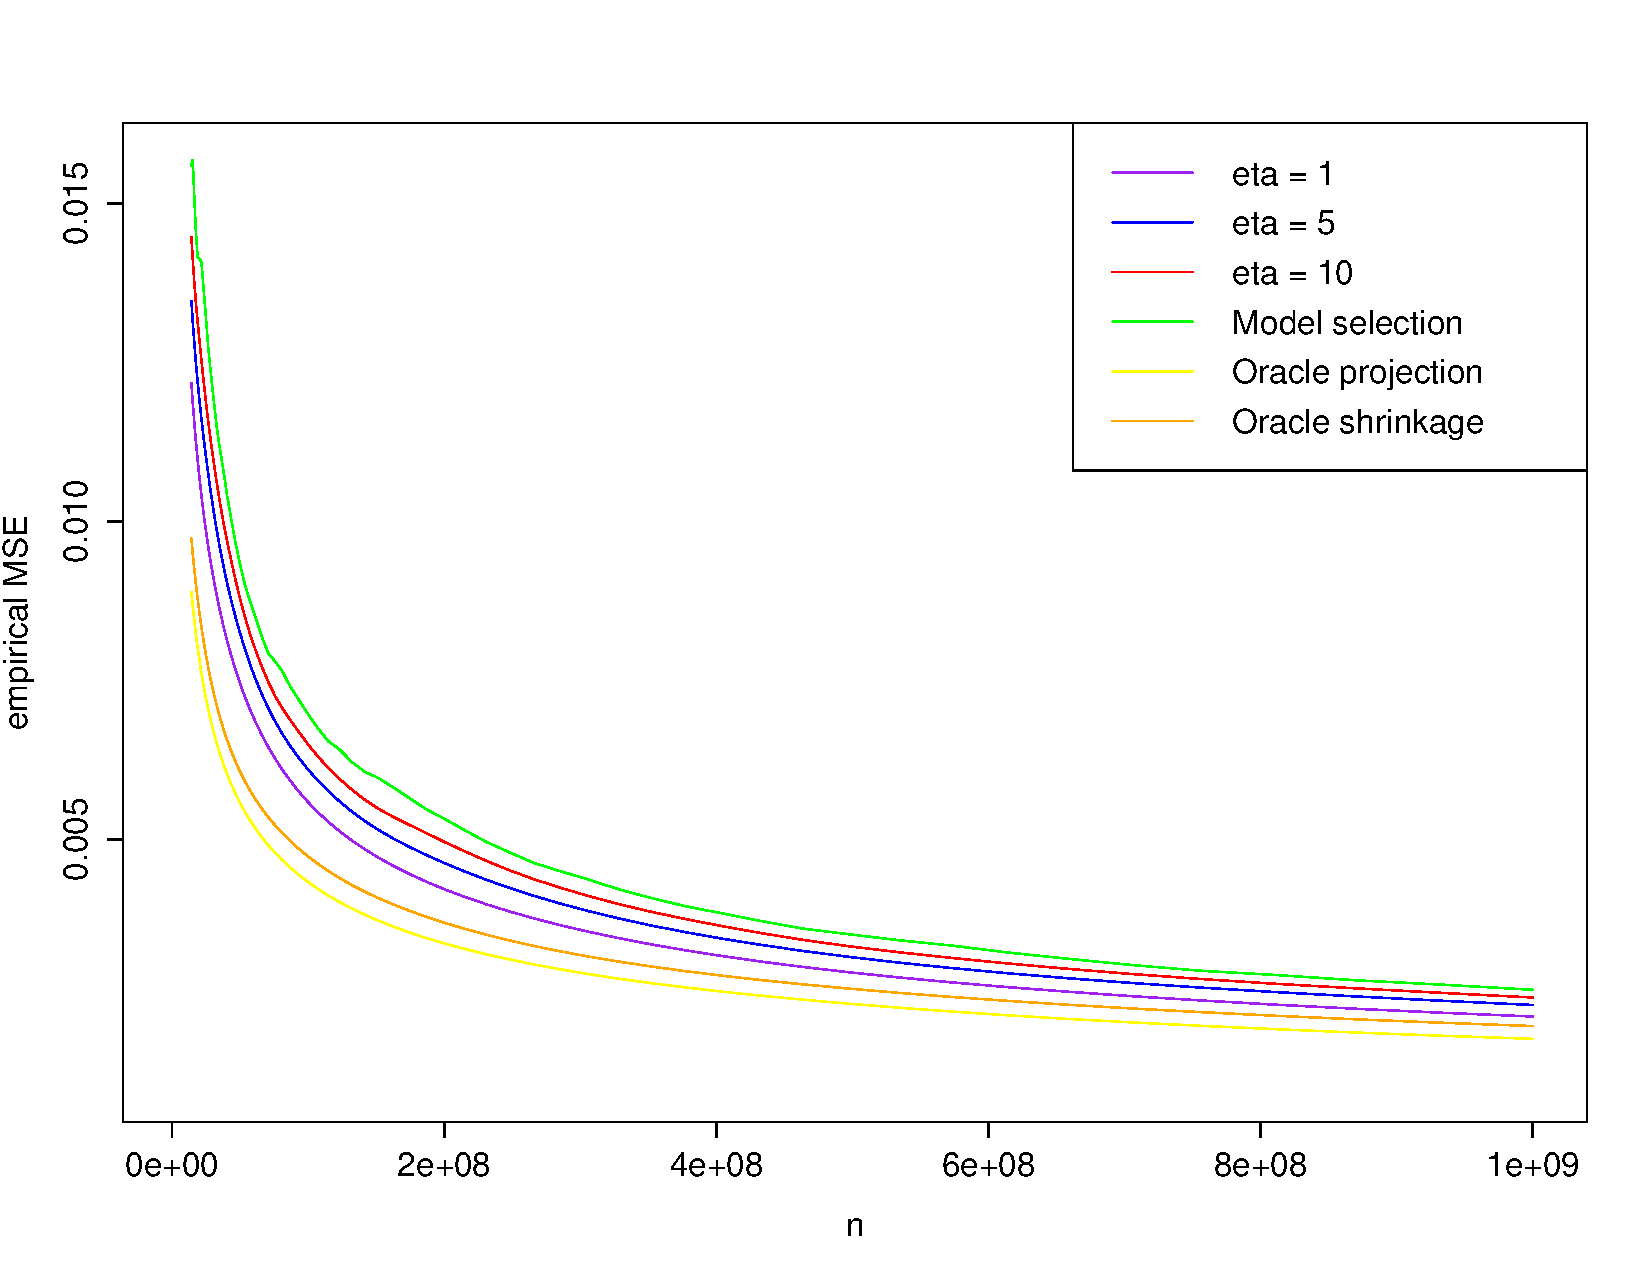
\includegraphics[width=1.\linewidth]{EQM1.pdf}
  \caption{$\theta^{\circ}$ polynomial and $\lambda$ polynomial}
  \label{fig3:sub1}
\end{subfigure}%
\begin{subfigure}{.5\textwidth}
  \centering
  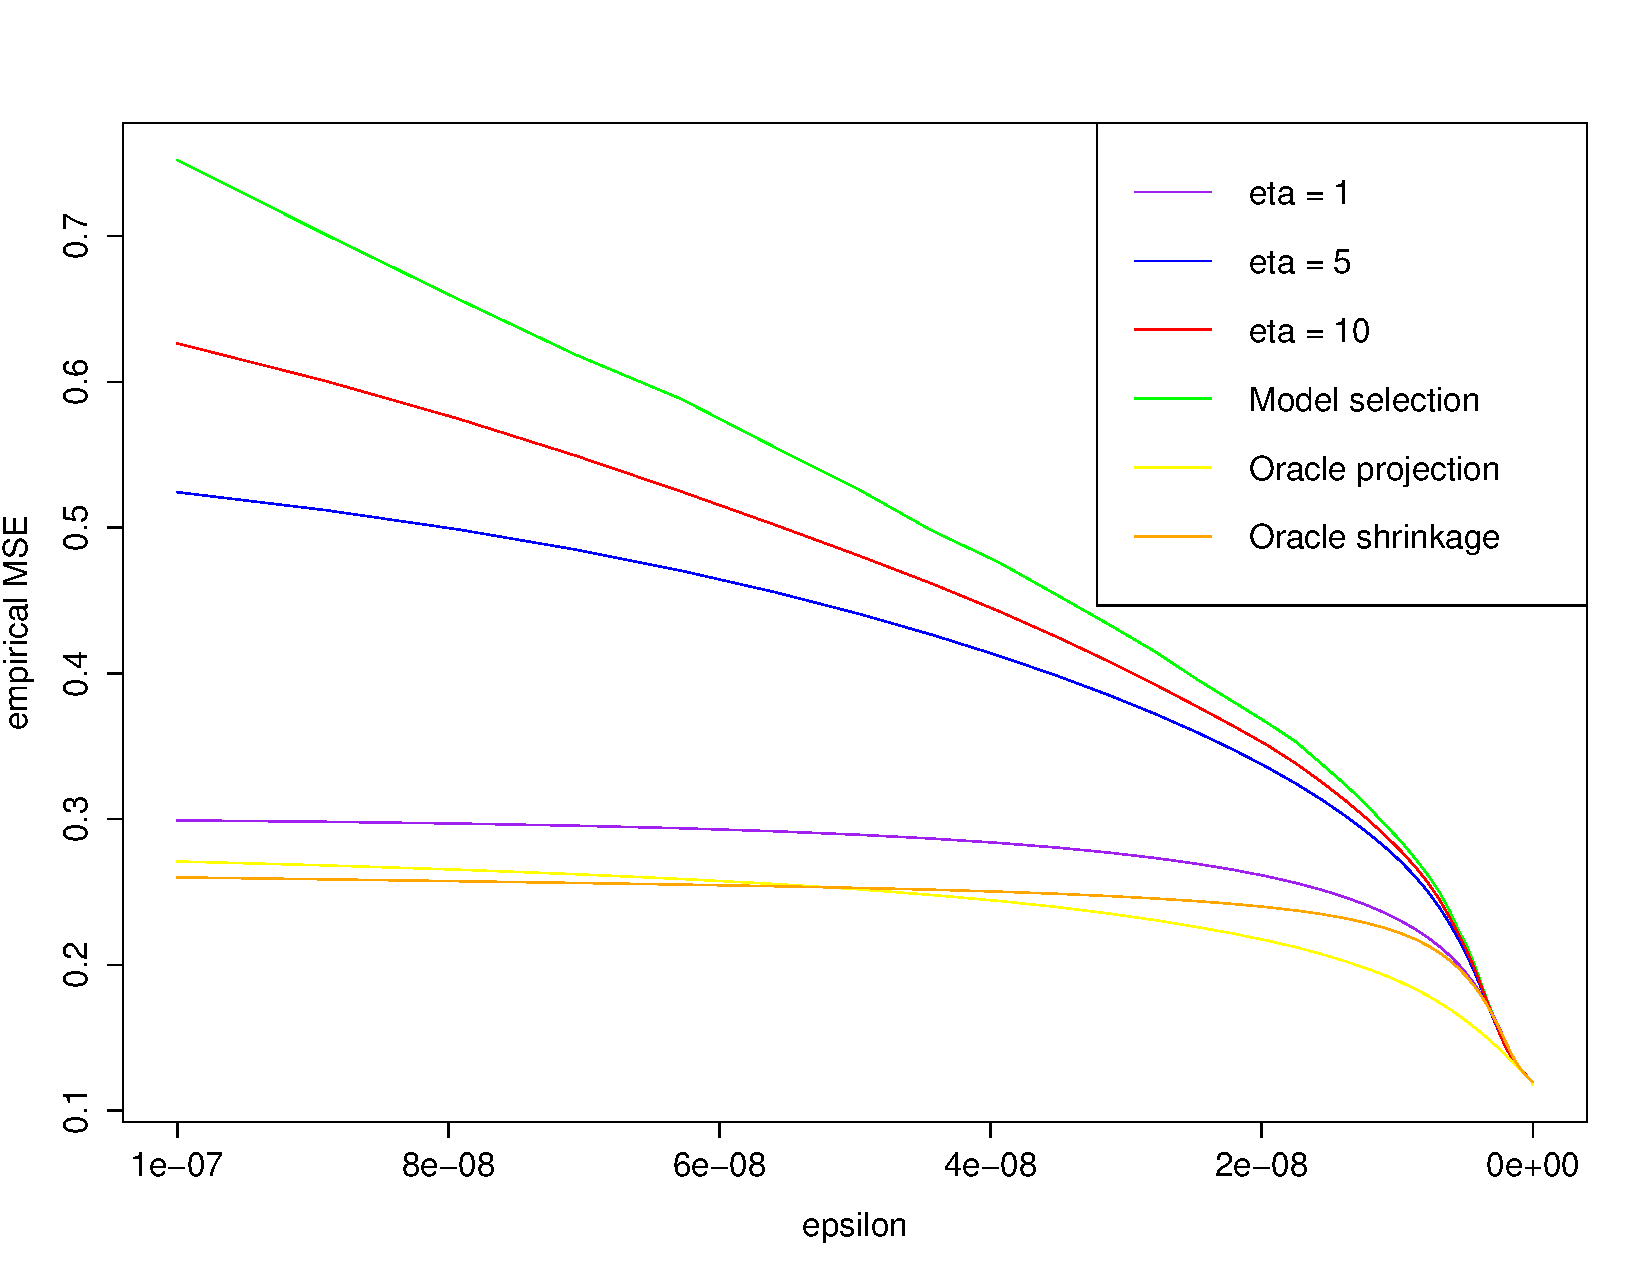
\includegraphics[width=1.\linewidth]{EQM2.pdf}
  \caption{$\theta^{\circ}$ polynomial and $\lambda$ exponential}
  \label{fig3:sub2}
\end{subfigure}
\begin{subfigure}{.5\textwidth}
  \centering
  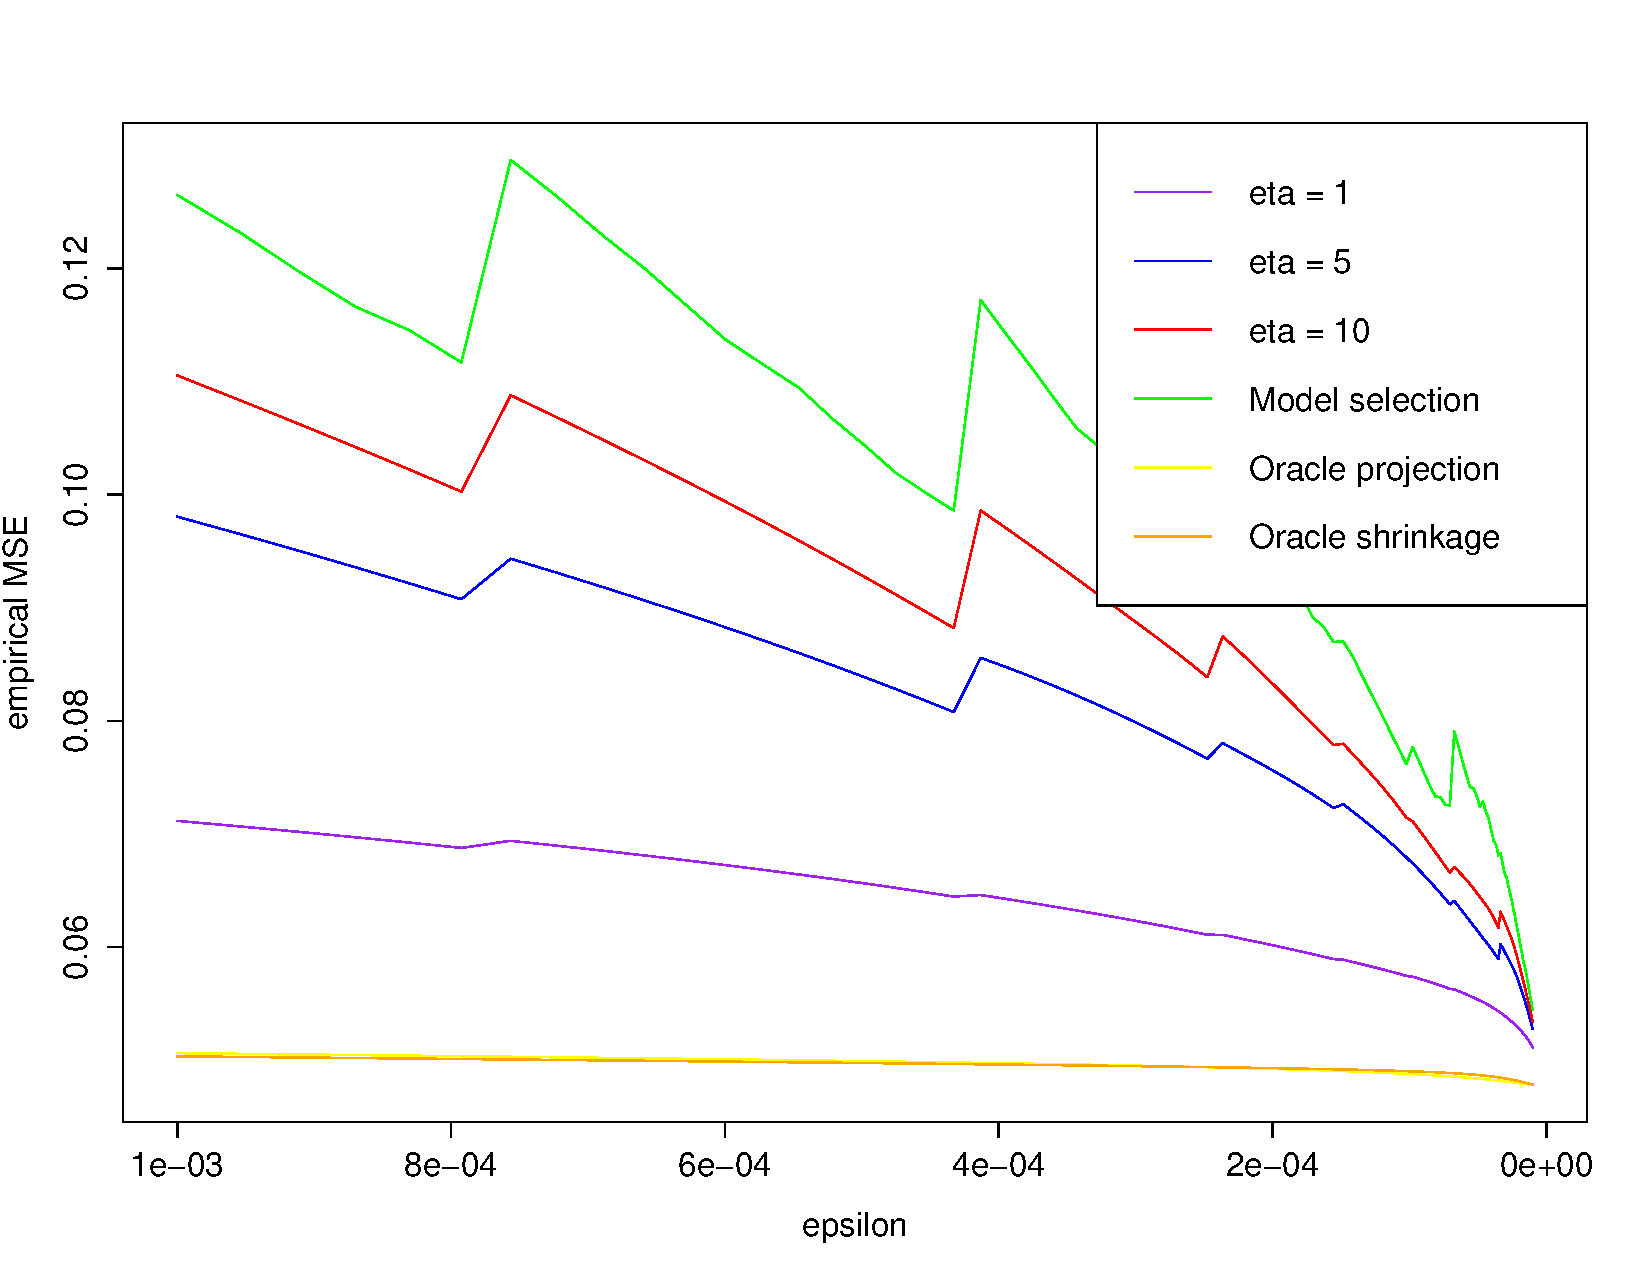
\includegraphics[width=1.\linewidth]{EQM3}
  \caption{$\theta^{\circ}$ exponential and $\lambda$ polynomial}
  \label{fig3:sub3}
\end{subfigure}%
\begin{subfigure}{.5\textwidth}
  \centering
  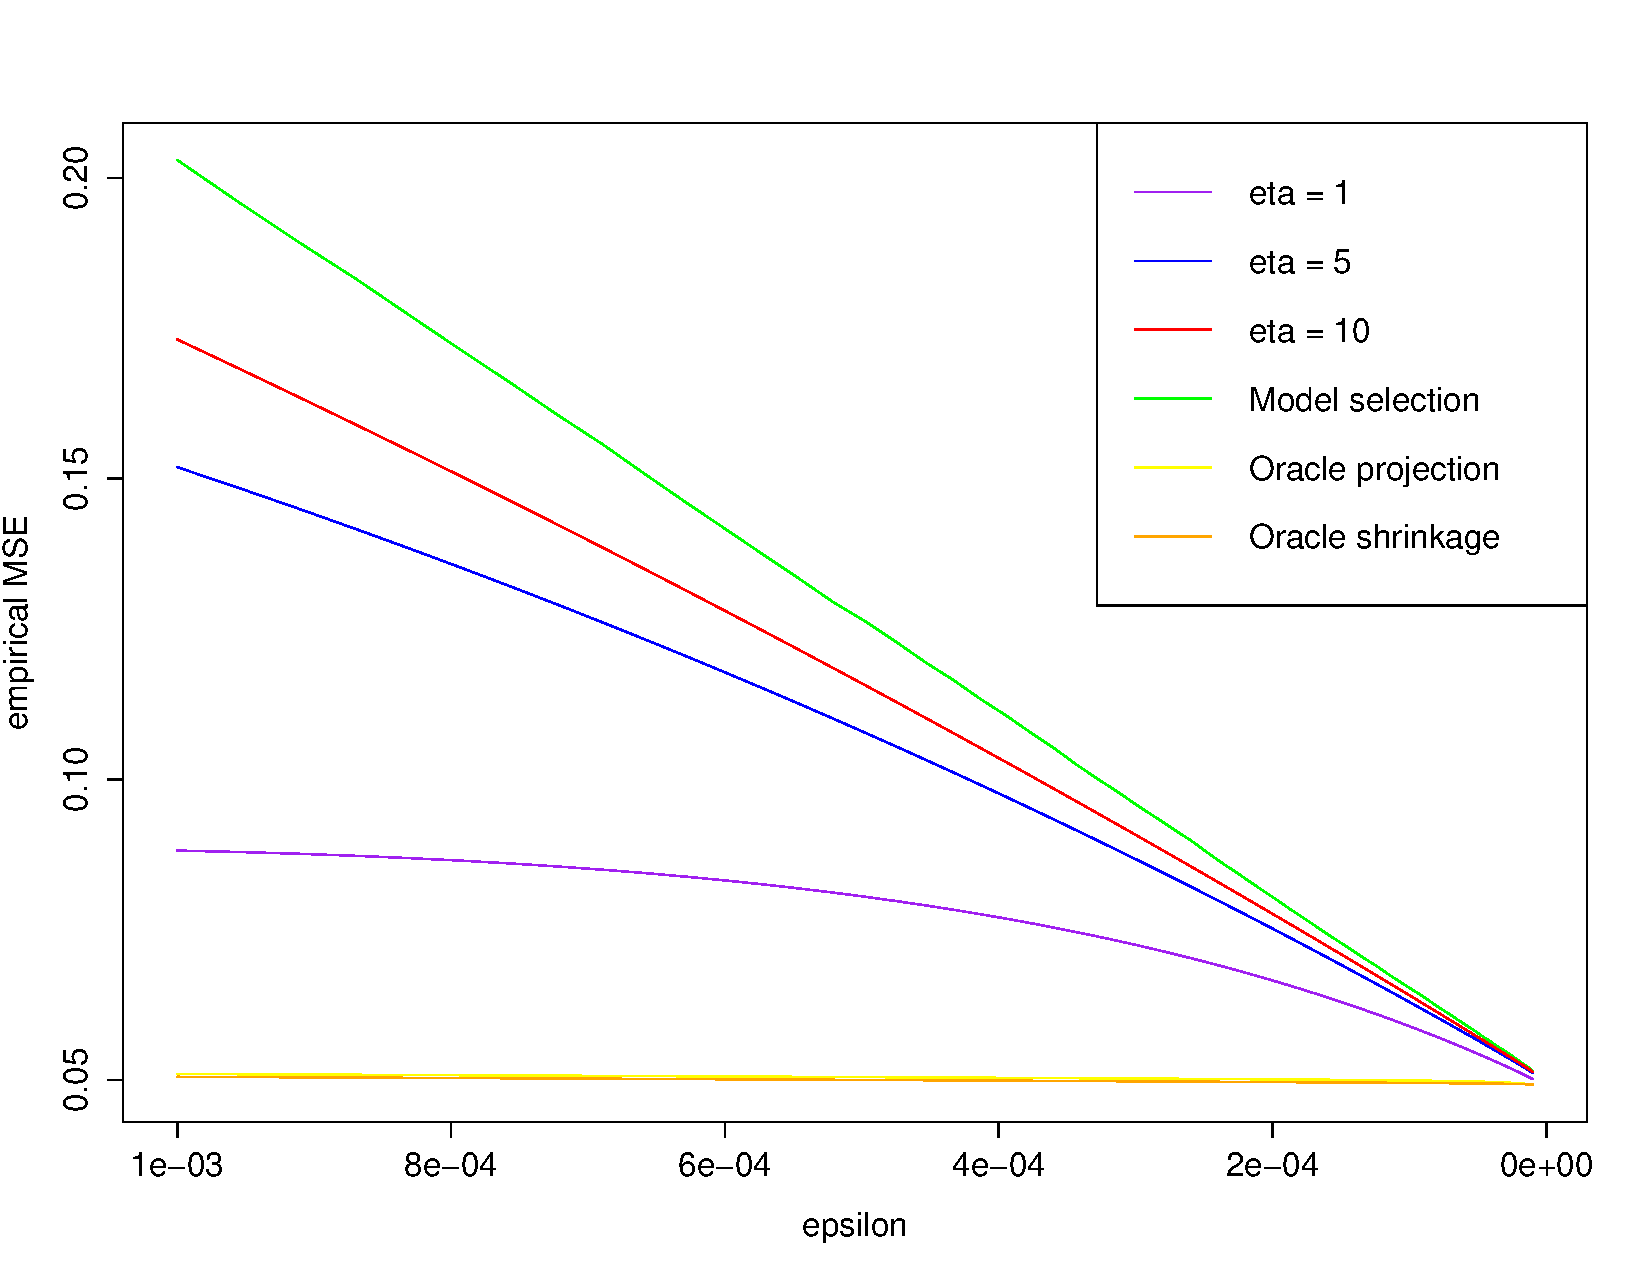
\includegraphics[width=1.\linewidth]{EQM4}
  \caption{$\theta^{\circ}$ exponential and $\lambda$ exponential}
  \label{fig3:sub4}
\end{subfigure}
\caption{Estimated median of the quadratic error of the estimator given by the posterior mean for different classes of $\theta^{\circ}$ and $\lambda$ with $\theta^{\times} \equiv 0$ and $s \equiv 1$.}
\label{EQM}
\end{figure}

%
%\chapter*{List of notations}

\section*{Spaces}
\subsection*{General case}
\begin{alignat*}{3}
& \left(\mathds{Y}, \mathcal{Y}\right) &&: && \quad \text{the measurable space of observations};\\
& \mathds{T} \subset \R &&: && \quad \text{time domain};\\
& \mathds{D} \subset \R &&: && \quad \text{intensity domain};\\
& \Xi = \left\{f : \mathds{T} \rightarrow \mathds{D}\right\} &&: && \quad \text{the parameter space represented in time domain};\\
& \mathds{F} \subset \R &&: && \quad \text{frequency domain};\\
& \mathds{A} \subset \C &&: && \quad \text{amplitude in frequency domain};\\
& \left(\Theta, \mathcal{B}\right) = \left(\left\{\theta : \mathds{F} \rightarrow \mathds{A}\right\}, \mathcal{B}\right) &&: && \quad \text{the parameter space represented in frequency domain};
\end{alignat*}

\subsection*{Inverse Gaussian sequence space model}
\begin{alignat*}{3}
%& \left([0, 1[, \mathcal{A}\right) &&: && \quad \text{the measurable space of observations};\\
%& \mathcal{D}_{\mu}([0,1[) && : && \quad \text{space of densities on } [0, 1[ \text{ with respect to } \mu ;\\
& \mathcal{M}([0, 1[) && : && \quad \text{space of probability measures on } [0, 1[\\
& \mathcal{S}^{+}(\mathds{Z}) && : && \quad \text{ set of all positive definite, complex valued functions } [f] \text{ on } \mathds{Z} \text{ with } [f](0) = 1;\\
\end{alignat*}

\subsection*{Circular density deconvolution model}
\begin{alignat*}{3}
%& \left([0, 1[, \mathcal{A}\right) &&: && \quad \text{the measurable space of observations};\\
%& \mathcal{D}_{\mu}([0,1[) && : && \quad \text{space of densities on } [0, 1[ \text{ with respect to } \mu ;\\
& \mathcal{M}([0, 1[) && : && \quad \text{space of probability measures on } [0, 1[\\
& \mathcal{S}^{+}(\mathds{Z}) && : && \quad \text{ set of all positive definite, complex valued functions } [f] \text{ on } \mathds{Z} \text{ with } [f](0) = 1;\\
\end{alignat*}

\section*{Measures and densities}

\subsection*{General case}
\begin{alignat*}{5}
& \P_{\boldsymbol{\theta}^{m}} &&:&& \mathcal{B} \rightarrow [0,1])_{f \in \Xi} &&:&& \quad \text{Gaussian sieve prior with threshold parameter }m\\
\end{alignat*}


$\P_{\boldsymbol{\theta}^{M}}$

$\P_{M}$

$\P_{M \vert Y^{n}}^{n, (\eta)}$

$\P_{\boldsymbol{\theta}^{m}\vert Y^{n}}^{n, (\eta)}$

$\P_{\boldsymbol{\theta}^{M}\vert Y^{n}}^{n, (\eta)}$

\subsection*{Inverse Gaussian sequence space model}
\subsection*{Circular density deconvolution model}

\begin{alignat*}{5}
& (\mathds{P}_{Y \vert f} &&:&& \mathcal{Y} \rightarrow [0,1])_{f \in \Xi} &&:&& \quad \text{family to which the data distribution belongs}\\
& \mathds{P}^{X} &&:&& \mathcal{A} \rightarrow [0,1] &&: && \quad \text{distribution of interest};\\
& \mathds{P}^{\epsilon}&&:&& \mathcal{A} \rightarrow [0,1] &&: && \quad \text{distribution of the noise};\\
& \mu&&:&& \mathcal{A} \rightarrow \mathds{R}_{+} &&: && \quad \text{ a sigma-finite measure, dominating both } \mathds{P}^{X} \text{ and } \mathds{P}^{\epsilon};\\
& f^{X}&&:&& [0, 1[ \rightarrow \overline{\mathds{R}_{+}} &&: && \quad \text{density of } \mathds{P}^{X} \text{ with respect to } \mu;\\
& f^{\epsilon}&&:&& [0, 1[ \rightarrow \overline{\mathds{R}_{+}} &&: && \quad \text{density of } \mathds{P}^{\epsilon} \text{ with respect to } \mu;\\
& \mathds{P}^{Y} (=\mathds{P}^{X}*\mathds{P}^{\epsilon})&&:&& \mathcal{A} \rightarrow [0,1] &&: && \quad \text{distribution of the observations};\\
& f^{Y}(=f^{X}*f^{\epsilon})&&:&& [0, 1[ \rightarrow \overline{\mathds{R}_{+}} &&: && \quad \text{density of } \mathds{P}^{Y} \text{ with respect to } \mu;\\
& \# && : && \sigma(\mathcal{P}(G)) \rightarrow \N && : && \text{counting measure on the sigma-algebra generated by the set of subsets of} G
\end{alignat*}


\section*{Random variables}
\subsection*{General case}
\subsection*{Inverse Gaussian sequence space model}
\subsection*{Circular density deconvolution model}
\begin{alignat*}{5}
& X &&:&& (\Omega, \mathcal{B}) \rightarrow ([0,1[, \mathcal{A}) &&: && \quad \text{a random variable with distribution } \mathds{P}^{X};\\
& \epsilon &&:&& (\Omega, \mathcal{B}) \rightarrow ([0,1[, \mathcal{A})  &&: && \quad \text{a random variable with distribution } \mathds{P}^{\epsilon};\\
& Y (=X \Box \epsilon) &&:&& (\Omega, \mathcal{B}) \rightarrow ([0,1[, \mathcal{A})  &&: && \quad \text{a random variable with distribution } \mathds{P}^{Y};\\
& X^{n} (=(X^{n}_{i})_{i \in \llbracket 1, n \rrbracket}) &&:&& (\Omega, \mathcal{B}) \rightarrow ([0,1[^{n}, \mathcal{A}^{\otimes n}) &&: && \quad \text{a } n \text{-vector of i.i.d. replications of } X;\\
& \epsilon^{n} (=(\epsilon^{n}_{i})_{i \in \llbracket 1, n \rrbracket})&&:&& (\Omega, \mathcal{B}) \rightarrow ([0,1[^{n}, \mathcal{A}^{\otimes n}) &&: && \quad \text{a } n \text{-vector of i.i.d. replications of } \epsilon;\\
& Y^{n} (=(Y^{n}_{i})_{i \in \llbracket 1, n \rrbracket}) &&:&& (\Omega, \mathcal{B}) \rightarrow ([0,1[^{n}, \mathcal{A}^{\otimes n})  &&: && \quad \text{a } n \text{-vector of i.i.d. replications of } Y;\\
& \boldsymbol{\theta}^{m} &&:&& (\Omega, \mathcal{B}) \rightarrow ([0,1[, \mathcal{A}) &&: && \quad \text{a random variable with distribution } \mathds{P}^{X};\\
& \boldsymbol{\theta}^{M} &&:&& (\Omega, \mathcal{B}) \rightarrow ([0,1[, \mathcal{A}) &&: && \quad \text{a random variable with distribution } \mathds{P}^{X};\\
& \widetilde{\theta}^{m, (\eta)} &&:&& (\Omega, \mathcal{B}) \rightarrow ([0,1[, \mathcal{A}) &&: && \quad \text{a random variable with distribution } \mathds{P}^{X};\\
& \widehat{\theta}^{(\eta)} &&:&& (\Omega, \mathcal{B}) \rightarrow ([0,1[, \mathcal{A}) &&: && \quad \text{a random variable with distribution } \mathds{P}^{X};\\
& \bar{\theta}^{m, (\eta)} &&:&& (\Omega, \mathcal{B}) \rightarrow ([0,1[, \mathcal{A}) &&: && \quad \text{a random variable with distribution } \mathds{P}^{X};
\end{alignat*}

\section*{Unary operators}
\subsection*{General case}
\subsection*{Inverse Gaussian sequence space model}
\subsection*{Circular density deconvolution model}
\begin{alignat*}{6}
& &&\mathds{E}[\cdot] && && &&:&& \quad \text{the expectation operator when the distribution is obvious};\\
& \forall \mathds{P} \text{ distribution } && \mathds{E}_{\mathds{P}}[\cdot] && && &&:&& \quad \text{the expected value under } \mathds{P};\\
& && ^{*}\cdot &&:&& \mathcal{M}([0, 1[) && \rightarrow && \mathcal{M}([0, 1[);\\
& && && && \mathds{P} && \mapsto && ^{*}\mathds{P} = \mathds{P}*\mathds{P}^{\epsilon}\\
& && ^{*}\cdot &&:&& \mathcal{D}_{\mu}([0, 1[) && \rightarrow && \mathcal{D}_{\mu}([0, 1[);\\
& && && && f && \mapsto && ^{*}f = f*f^{\epsilon}\\
& \forall j \in \mathds{Z} && e_{j}(\cdot) &&:&& [0,1[ && \rightarrow && \mathds{C};\\
& && && && x && \mapsto && \exp[-2 i \pi j x]\\
& && \mathcal{F}_{\mu}(\cdot) &&:&& \mathcal{D}_{\mu}([0, 1[) && \rightarrow && \mathcal{S}^{+}(\mathds{Z});\\
& && && && f && \mapsto && [f] = \left(j \mapsto \int_{0}^{1} f(x) e_{j}(x) d\mu(x)\right)\\
& && \mathcal{F}(\cdot) &&:&& \mathcal{M}([0, 1[) && \rightarrow && \mathcal{S}^{+}(\mathds{Z});\\
& && && && \mathds{P} && \mapsto && [\mathds{P}] = \left(j \mapsto \int_{0}^{1} e_{j}(x) d\mathds{P}(x)\right)\\
& && \mathcal{F}_{\mu}^{-1}(\cdot) &&:&& \mathcal{S}^{+}(\mathds{Z}) && \rightarrow && \mathcal{D}_{\mu}([0, 1[);\\
& && && && [f] && \mapsto && f = \left(x \mapsto \sum\limits_{j \in \mathds{Z}} [f]_{j} e_{j}(x) \right)\\
& && \mathcal{F}^{-1}(\cdot) &&:&& \mathcal{S}^{+}(\mathds{Z}) && \rightarrow && \mathcal{M}([0, 1[);\\
& && && && [\mathds{P}] && \mapsto && \mathds{P} = \left(A \mapsto \int_{A} \sum\limits_{j \in \mathds{Z}} [\mathds{P}]_{j} e_{j}(x) dx\right)\\
\end{alignat*}

\section*{Binary operators}
\subsection*{General case}
\subsection*{Inverse Gaussian sequence space model}
\subsection*{Circular density deconvolution model}
\begin{alignat*}{7}
& \cdot \Box \cdot &&:&& [0,1[^{2} &&\rightarrow&& [0,1[ &&: && \quad \text{the modular addition binary operator on the unit segment};\\
& && && (x,y) &&\mapsto&& x+y-\lfloor x+y \rfloor && &&\\
\end{alignat*}

\section*{Miscellaneous}
\subsection*{General case}
\subsection*{Inverse Gaussian sequence space model}
\subsection*{Circular density deconvolution model}
For any set $S$, subset $s \subseteq S$ we note $\mathds{1}_{s}$ the indicatrix function
\begin{alignat*}{5}
	&\mathds{1}_{s} &&:&& S &&\rightarrow&& \{0, 1\};\\
	& && && x && \mapsto &&
		\begin{cases}
			0 \text{ if } x \notin s\\
			1 \text{ if } x \in s
		\end{cases}
\end{alignat*}

















\bibliography{biblio.bib}{}
\nocite{*}
\bibliographystyle{apalike}
%

\end{document}
%%% Local Variables:
%%% mode: latex
%%% TeX-master: t
%%% End:
